\documentclass[11pt,a4paper,oneside]{book}
% Leeds SoC MSc dissertation — ported from the official LaTeX template (Prepare/template-2),
% font size set to 11pt per the written rule in SoC-report-Template.docx.
\usepackage{setspace}
\usepackage{geometry}
\usepackage[toc]{appendix}
\usepackage[T1]{fontenc}
\usepackage{textcomp}
\usepackage{graphicx}
% The appendices are figure-dense, and tbp floats queue up and drift across
% section boundaries -- one was measured eight pages downstream, landing in a
% section it does not illustrate. The [section] option is not used: it would
% fence the chapters too, and the main text has no page to spare at its 60-page limit.
% \FloatBarrier is placed by hand before each appendix section instead.
\usepackage{placeins}
\usepackage{titlesec}
\usepackage{booktabs}
\usepackage{multirow}
\usepackage{array}
\usepackage{amsmath}
\usepackage{microtype}
\usepackage{tikz}
\usetikzlibrary{arrows.meta,positioning,shapes.geometric}
\usepackage[hidelinks,bookmarksnumbered=true]{hyperref}
% Long dataset URLs in the bibliography cannot break without this and stretch
% their neighbouring lines to visibly gappy inter-word spacing.
\usepackage{xurl}
% xurl permits a break at any character, which keeps the reference list free
% of overfull lines but split the Yelp URL mid-word as "open-datas / et/".
% The bibliography carries exactly two URLs, of 54 and 47 characters, so the
% break points can be confined to punctuation without risking an overfull
% line; the build gate counts overfull boxes and would catch a regression.
\def\UrlBreaks{\do\/\do\-\do\.\do\_\do\?\do\=\do\&}

% Float and caption geometry sized against the regenerated figures (W3).
% ---------------------------------------------------------------------------
% Float and caption geometry for the A4 text block.
%
% The eleven figures are regenerated at dissertation geometry by
% scripts/analysis/diss_figs/regen.py (canvas only -- no figure content is
% redrawn); this file is the other half of the same job, and the two are sized
% against each other.  Text block: 160 mm x 252 mm = 455.24 pt x 717.01 pt.
%
% Captions.  Set at \small and single spaced.  The 11pt / one-and-a-half-spaced
% rule governs the body of the report; a caption is a label, and these captions
% are long (six to nine lines each) because they carry the basis, denominator
% and does-not-show prose that keeps every figure readable on its own.  At body
% size and body spacing those nine lines cost 149 pt -- a fifth of the page --
% on top of a figure that already fills most of it, which is what pushed eight
% floats past the page height and gave the "Float too large" warnings.
%
% Float fractions.  The eleven composites that used to fill this block have been
% cut into eighteen parts by scripts/analysis/diss_figs/split_panels.py -- twenty
% main-text figures in all -- so the floats now measure 0.20--0.58 of the text
% height instead of 0.82--0.98.  Two of the eleven survive whole: F4, whose right column runs the full height so it has no
% horizontal seam, and F12, whose panel-(a) note abuts the panel-(b) heading with
% no gap at any canvas the generator will draw.
%
% The raised ceilings below are what let two of the new parts sit at one page top
% with body text beneath them, which is the conventional look and the page
% saving; \textfraction is the guarantee that goes with it, and
% \floatpagefraction is set high so a float page is built only when floats really
% do fill one -- lowering it costs pages, because it lets LaTeX spend a whole page
% on floats that would otherwise have shared a page with text.
% ---------------------------------------------------------------------------

\usepackage[font={small,singlespacing},skip=5pt,justification=justified]{caption}

% Floats may occupy more of a page than the stock report defaults allow.
\renewcommand{\topfraction}{0.92}        % max page fraction for top floats
\renewcommand{\bottomfraction}{0.85}     % max page fraction for bottom floats
\renewcommand{\textfraction}{0.07}       % min page fraction that must be text
\renewcommand{\floatpagefraction}{0.95}  % min fill before a float page is used
\setcounter{topnumber}{3}
\setcounter{bottomnumber}{1}
\setcounter{totalnumber}{4}

% Tighter separation between a float and the text it interrupts; the stock
% 20 pt above and below a page-wide float is generous for a 252 mm block.
\setlength{\textfloatsep}{12pt plus 2pt minus 4pt}
\setlength{\floatsep}{10pt plus 2pt minus 2pt}
\setlength{\intextsep}{10pt plus 2pt minus 2pt}


\newcommand{\projectTitle}{SP500Vol-Bench: A Point-in-Time Benchmark and Identity-Controlled Audit of Disclosure-Based Volatility Forecasting}
\newcommand{\fullname}{Kun Zhang}
\newcommand{\degreeTitle}{MSc Advanced Computer Science}
\newcommand{\session}{2025/26}

% Document properties. hyperref is loaded above, but pdftitle and pdfauthor
% have to expand the four macros defined immediately above this line, so the
% metadata is set here rather than in the package options.
\hypersetup{%
  pdftitle={\projectTitle},
  pdfauthor={\fullname},
  pdfsubject={\degreeTitle{} dissertation, School of Computer Science, University of Leeds},
  pdfkeywords={volatility forecasting; corporate disclosure; point-in-time benchmark; incremental value}%
}

% 25 mm binding edge (official Leeds LaTeX template geometry)
\geometry{a4paper, left=25mm, right=25mm, top=25mm, bottom=20mm}
\onehalfspacing

\titleformat{\chapter}[display]
   {\normalfont\Huge\bfseries}{\vspace*{-1\baselineskip}\chaptertitlename\ \thechapter}{15pt}{\huge}
\titlespacing*{\chapter}{0pt}{0pt}{15pt}

\renewcommand\bibname{References}
\bibliographystyle{abbrv}
\DeclareTextCommandDefault{\textcopyright}{\textcircled{c}}

\newenvironment{dissertationsummary}
 {\cleardoublepage \null \begin{center}\textbf{Summary}\end{center}}
 {\vfill \null}

\newcommand{\frontcover}{ \begin{titlepage}
\newgeometry{left=25mm,right=25mm,top=45mm,bottom=0.1cm}
\pdfbookmark[0]{Title Page}{fm:titlepage}
\noindent
\begin{minipage}[t]{8cm}
\textbf{\Large{School of Computer Science}}\\
{\fontfamily{ptm}\selectfont \uppercase{faculty of engineering and \\physical sciences}}
\end{minipage}
\hfill
\begin{minipage}[t]{7cm}
\raggedleft
\includegraphics[scale=0.2]{logo_black.png}
\end{minipage}
\noindent\makebox[\linewidth]{\rule{\paperwidth}{0.4pt}}
\begin{center}
\vspace*{37mm}
\textbf{\Large\projectTitle}\\[10mm]
\textbf{\large\fullname}\\[10mm]
\textbf{Submitted in accordance with the requirements for the degree of}\\
\textbf{\degreeTitle}\\[10mm]
\session
\end{center}
\restoregeometry
\end{titlepage} }

\begin{document}
\pagenumbering{roman}
\frontcover
% The titlepage environment resets the page counter at its close, so without
% this the title page and the page after it are both numbered i and hyperref
% emits a duplicate page.i destination.
\setcounter{page}{2}
\clearpage
\pdfbookmark[0]{Submitted Items and Declaration}{fm:declaration}
\noindent The candidate confirms that the following have been submitted.\\[4mm]
\begin{center}
\begin{tabular}{|p{52mm}|p{38mm}|p{52mm}|}
\hline
\textbf{Items} & \textbf{Format} & \textbf{Recipient(s) and Date} \\\hline
Deliverable 1 (SP500Vol-Bench: accession index, split definition, datasheet, licence-free variant) & Data (repository) & Supervisor, Assessor (31/08/26) \\\hline
Deliverable 2 (audit protocol, registered analysis records, aggregate evidence tables, power calibration) & Data (repository)\newline / Report & Supervisor, Assessor (31/08/26) \\\hline
Deliverable 3 (run-fingerprint chain for all 240 production runs, with verification script) & Code (repository) & Supervisor, Assessor (31/08/26) \\\hline
Deliverable 4 (code repository: regeneration pipeline and test suite) & Code (repository) & Supervisor, Assessor (31/08/26) \\\hline
Deliverable 5 (this dissertation) & Report & SSO (31/08/26) \\\hline
\end{tabular}
\end{center}
\vspace{3mm}
% The Format column says "repository"; without the address that is a
% direction with no destination, and this page is where the delivery is
% asserted. Appendix A carried the only other copy of the URL, 68 printed
% pages away.
\noindent Deliverables 1 to 4 are shared through the public repository at
\url{https://github.com/Beiciccc/sp500vol-bench}, inventoried in
Appendix~\ref{app:external}.
\vspace{5mm}

\noindent Type of project: \textbf{Empirical Investigation}\\[8mm]
\noindent The candidate confirms that the work submitted is their own and the appropriate credit has been given where reference has been made to the work of others.\\[4mm]
\noindent I understand that failure to attribute material which is obtained from another source may be considered as plagiarism.\\[10mm]
% Signature.  Drop a transparent PNG at figures/signature.png and it is set on
% the rule; with no such file the blank rule is typeset exactly as before, so
% the build never depends on a file that is not in the repository.  It is put
% here rather than annotated onto main.pdf because every gated rebuild
% regenerates that file and would silently discard an annotation.
\begin{flushright}
(Signature of Student)
\IfFileExists{figures/signature.png}{%
  % The image is cropped to the ink, and the baseline of "Kun Zhang" sits at
  % 48 per cent of its height -- the rest is the descender of the g.  Dropping
  % it by 52 per cent of 22.1mm therefore lands that baseline on the rule and
  % lets the descender hang below it, as a signature on a line does.  Zero
  % height and depth so the front matter's layout does not move.
  \makebox[50mm][c]{\raisebox{-11.5mm}[0pt][0pt]{%
    \includegraphics[width=42mm,keepaspectratio]{figures/signature.png}}}%
  \hspace*{-50mm}\rule{50mm}{1pt}%
}{%
  \rule{50mm}{1pt}%
}
\end{flushright}
\vfill
\begin{center}\textcopyright~\session~The University of Leeds and~\fullname\end{center}
\clearpage
\begin{dissertationsummary}
\pdfbookmark[0]{Summary}{fm:summary}
% Rebuilt 2026-08-02 (W2) from the frozen story per DISSERTATION_ARCHITECTURE.md;
% the June summary is retired in full (dossier Part 3: rewrite entirely).
% This file is input inside prelude.tex's dissertationsummary environment;
% keep it as bare paragraphs (no wrapper of its own).
When a language model appears to beat a price-based benchmark at forecasting stock-market volatility, the gain may reflect not what a filing said but which firm filed it. This dissertation builds the instruments to tell those apart. The first is \mbox{SP500Vol-Bench}: a survivorship-free, point-in-time benchmark linking 144{,}129 SEC filings of S\&P~500 constituents over 2010--2025 to the volatility their filers subsequently realised, under a no-look-ahead protocol. % src: frozen 03_dataset.tex
The second is an identity-controlled audit crediting text only for the out-of-sample loss it removes beyond a recalibrated price reference, with day-clustered inference, placebo gates and power calibration. Across models from word counts to a prompted 32-billion-parameter language model, the audit returns a calibrated near-null. No challenger beats the price baseline standalone under squared error or volatility-unit QLIKE (0 of 180 comparisons; 7 of 180 favour a challenger in variance units, all seven price models). % src: results/tables/dm_pairwise_clustered.md (squared error: 0 of 180 better, 155 worse);
% results/tables/variance_unit_standalone180.csv (volatility-unit QLIKE 0 of 180; variance-unit
% 7 of 180, all A3/A4 price arms)
Apparent gains against the single recalibrated reference (38 of 69 cells) collapse to 8 against a reference that knows only who is filing, to 9 against a pool of five price models, and to 0 against both; those three counts are taken on the rows every rung of the ladder shares. % src: results/tables/m1_ensemble_primary.md; firm_identity_ensemble.md; maximal_reference_ensemble.md; control_intersection_ensemble.md
A zero-text term carrying each firm's average volatility, reading no text at all, improves on the recalibrated price baseline in four of six channel-horizon comparisons on those shared rows, and three of six over the full baseline panels. % src: results/tables/firm_identity_ensemble.csv (merged-grid basis, firm_beats_fR true in
% 4 of 6 channel-horizon comparisons); results/tables/firm_identity_control_zerotext.csv
% (all-A2-rows basis, 3 of 6; long-form h=5 is the comparison that moves)
An anonymisation arm prices the 8-K channel's identity share at a pooled median of 0.51 over both executed arms' six cells (0.56 for the prompted arm alone): roughly half of what survives the price reference is who filed rather than what was filed. % src: results/tables/anon_share_ci.md
What remains is a bounded residual --- prompted readings of 8-K filings retain 0.2--0.5 per cent over the firm-identity reference --- with no measurable portfolio value. % src: results/tables/firm_identity_ensemble.md; portfolio_econ.csv
The verdict is therefore an ordering rather than a number: on this panel disclosure text is detectable, only partially attributable to content, and not realisable as economic value.
The audit travels: on an external earnings-call corpus it reprices a published gain to nothing detectable, while on consumer reviews a content signal survives the same controls. % src: results/tables/maec_audit.md; yelp_multiarm.md
The benchmark's licence-free core, the audit protocol and its power calibration are released for reuse: a version-controlled regeneration pipeline behind 186 automated tests, with all 240 production runs cryptographically fingerprinted and every reported number traced to a committed evidence file.

\end{dissertationsummary}
\clearpage
\pdfbookmark[0]{Acknowledgements}{fm:acknowledgements}
\begin{center}\textbf{Acknowledgements}\end{center}
A year ago I had never published a paper. Since then I have written two with my
supervisor, Dr Chunwei Xia: an oral paper at NLPCC 2026 and a regular paper at
PRICAI 2026. With his guidance the work behind this dissertation went further
still, to a submission to AAAI 2027, which is not a step I would have thought to
take on my own. He taught me how to do research, and then he taught me where to
aim it. I am grateful for both, and for his patience while I learned.

\bigskip
\begin{flushright}
\emph{What's past is prologue.}\\[1mm]
{\footnotesize --- \emph{The Tempest}, II.i}
\end{flushright}

\clearpage
\pdfbookmark[0]{Contents}{fm:contents}
\tableofcontents
\clearpage
\pdfbookmark[0]{List of Tables}{fm:listoftables}
\listoftables
\clearpage
\pdfbookmark[0]{List of Figures}{fm:listoffigures}
\listoffigures
\clearpage
% Nomenclature. The official template (Prepare/template-2/prelude.tex) runs
% declaration, Summary, Acknowledgements, contents, optional lists, arabic; it
% neither prescribes nor forbids a nomenclature list, so this sits after the
% List of Figures. It is roman-numbered front matter and costs no main-text
% page. Like the Summary, the Acknowledgements and the two lists it takes a
% \pdfbookmark and no table-of-contents entry, and it is not a numbered table,
% so it stays out of the List of Tables.
\pdfbookmark[0]{Nomenclature}{fm:nomenclature}
% ---------------------------------------------------------------------------
% Nomenclature.  Front matter, placed after the List of Figures.
%
% Every entry is lifted from the place the report already defines it: the arm
% codes and the text-handling codes from the model matrix (Table
% tab:model-matrix and its caption), the counting vocabulary from the primary
% basis table (tab:res-basis) and from the reference-ladder and inference
% subsections of Chapter 3, and each abbreviation from its own first use.
% Nothing here may say anything the chapter does not; if a definition changes
% there, it changes here too.
%
% Provenance.  No number in this file is new: every one is a transcription of
% a chapter table or equation, so each group carries a single src comment on
% its own line naming that source, rather than a per-row evidence file.
%
% Format.  Five grouped tabulars rather than one long alphabetical list: the
% arm codes, the text-handling codes, the abbreviations, the notation and the
% vocabulary are five different kinds of lookup, and a reader arrives wanting
% one of them, not all five.  Plain tabulars rather than a longtable, because
% longtable is not loaded and config.tex is not this file's to edit; the page
% break falls between groups instead, which is where it should fall anyway.
% Splitting the 31-row abbreviation tabular so that it too could break was
% tried and reverted: it filled page one but left page two a sixth emptier,
% and it ended page one on a list with no closing rule.
%
% \noindent has to sit after \singlespacing, not before it.  setspace's
% \singlespacing forces vertical mode, which discards a \noindent issued ahead
% of it and lets the tabular start an indented paragraph 17 pt too wide.
%
% This list carries no \caption and is not a numbered table, so it does not
% enter the List of Tables.  Like the Summary, the Acknowledgements, the List
% of Tables and the List of Figures it takes a \pdfbookmark and no \toc entry.
% ---------------------------------------------------------------------------

\chapter*{Nomenclature}
% book's \chapter* leaves the previous \markboth standing, so without this the
% running head on this list's later pages reads LIST OF FIGURES.
\markboth{\MakeUppercase{Nomenclature}}{\MakeUppercase{Nomenclature}}

Model arms are named throughout by the codes of the model matrix
(Table~\ref{tab:model-matrix}), and every headline count is read against the
primary basis (Table~\ref{tab:res-basis}). The entries below transcribe those two
tables' own definitions, together with the terms fixed in
Sections~\ref{sec:design-ladder} and~\ref{sec:design-inference}; the chapter
that defines a term remains the authority on it.

\vspace{2mm}
\noindent\textbf{Arm codes.} The four blocks of the model matrix.
\par\nobreak
\vspace{1mm}
% src: chapters/03_datasets_and_experimental_design.tex, Table tab:model-matrix (ID and Model columns, transcribed)
{\small\singlespacing
\noindent\begin{tabular}{@{}>{\raggedright\arraybackslash}p{0.09\textwidth}>{\raggedright\arraybackslash}p{0.87\textwidth}@{}}
\toprule
A1 & Naive historical volatility \\
A2 & HAR-RV (primary baseline) \\
A3 & GARCH(1,1) \\
A4 & EGARCH \\
A5 & ARIMA on log-RV \\
A6 & SHAR and HARQ ($\times$2): realised semivariance, and the correction for measurement error in the realised-variance regressor \\
A7 & HAR-X, point-in-time log VIX \\
\midrule
B1 & Bag-of-words + ridge \\
B2 & TF--IDF + ridge \\
B3 & Loughran--McDonald dictionary, linear \\
B4 & Loughran--McDonald + engineered features \\
\midrule
C1 & BERT-base \\
C2 & FinBERT \\
C3 & RoBERTa-base \\
C4 & Longformer-4096 \\
C5 & Frozen LLM embeddings ($\times$3) \\
C5x & Qwen3-Emb.-8B, input parity, long-form \\
C6 & Prompted Qwen3-32B \\
\midrule
D1 & Concatenation MLP \\
D2 & Gated fusion \\
D3 & Price + C5 embedding ($\times$3) \\
D4 & Price + C6 forecast, in-prompt \\
\bottomrule
\end{tabular}\par
}

\vspace{3mm}
\noindent\textbf{Text handling.} How a model meets a document, from the same matrix.
\par\nobreak
\vspace{1mm}
% src: chapters/03_datasets_and_experimental_design.tex, Table tab:model-matrix caption (text-handling key, transcribed)
{\small\singlespacing
\noindent\begin{tabular}{@{}>{\raggedright\arraybackslash}p{0.13\textwidth}>{\raggedright\arraybackslash}p{0.83\textwidth}@{}}
\toprule
S1 & Truncation to the first 512 tokens \\
S2 & Chunk-mean pooling \\
S3 & Learned chunk attention \\
S4 & Hierarchical chunk encoder \\
S5 & Native 4{,}096-token context \\
\midrule
full text & Untruncated document (classical vectorisers) \\
4{,}096 tok. & The length the three frozen embedders were run at, an A100-40G budget rather than a model limit \\
excerpts & The curated excerpts read by the prompted arm (risk and MD\&A items for 10-K and 10-Q, head truncation otherwise; 8-K in full to a character budget) \\
\bottomrule
\end{tabular}\par
}

\vspace{3mm}
\noindent\textbf{Abbreviations.}
\par\nobreak
\vspace{1mm}
% src: each entry from its own first use in chapters/02_background.tex, chapters/03_datasets_and_experimental_design.tex or chapters/04_results.tex
{\small\singlespacing
\noindent\begin{tabular}{@{}>{\raggedright\arraybackslash}p{0.11\textwidth}>{\raggedright\arraybackslash}p{0.85\textwidth}@{}}
\toprule
10-K & Annual report \\
10-Q & Quarterly report \\
8-K & Current report, announcing a material event within days of its occurrence \\
ARIMA & Autoregressive integrated moving average (arm A5, fitted to log RV) \\
CCM & CRSP/Compustat-Merged, the WRDS-maintained crosswalk between CRSP securities and Compustat/SEC registrants \\
CIK & Central Index Key, the SEC's identifier for a registered filer \\
CRSP & Center for Research in Security Prices \\
DM & Diebold--Mariano, the test for equal forecast accuracy \\
EDGAR & The SEC's public full-text disclosure archive \\
EGARCH & Exponential GARCH (arm A4) \\
GARCH & Generalised autoregressive conditional heteroskedasticity (arm A3) \\
GPU & Graphics processing unit; training cost is reported in GPU-hours \\
HAC & Heteroskedasticity- and autocorrelation-consistent, the variance estimator the DM test uses \\
HAR & Heterogeneous autoregressive \\
HAR-RV & The heterogeneous autoregressive model of realised volatility (arm A2) \\
HARQ & HAR corrected for measurement error in the realised-variance regressor (arm A6, beside SHAR) \\
HAR-X & HAR augmented with the point-in-time log VIX (arm A7) \\
LLM & Large language model \\
MAEC & The published earnings-call corpus used as an external portability panel \\
MCS & Model confidence set \\
MD\&A & Management's discussion and analysis, the narrative results section of a 10-K or 10-Q \\
MDE & Minimum detectable effect: the smallest relative QLIKE improvement a cell's test would detect with 80 per cent power \\
MLP & Multilayer perceptron \\
PERMNO & CRSP's permanent security identifier, stable across ticker changes and renames \\
QLIKE & The quasi-likelihood loss, $y/f - \ln(y/f) - 1$ for proxy $y$ and forecast $f$ \\
RV & Realised volatility \\
SEC & United States Securities and Exchange Commission \\
SHAR & Realised-semivariance HAR (arm A6) \\
SPA & Superior predictive ability, Hansen's joint test \\
TF--IDF & Term frequency--inverse document frequency, a word-weighting scheme that discounts ubiquitous words \\
VIX & The market's option-implied volatility index \\
WRDS & Wharton Research Data Services \\
\bottomrule
\end{tabular}\par
}

\vspace{3mm}
\noindent\textbf{Notation.}
\par\nobreak
\vspace{1mm}
% src: chapters/03_datasets_and_experimental_design.tex, Eq. eq:data-rv and Eq. eq:m1 with the prose that defines their terms
{\small\singlespacing
\noindent\begin{tabular}{@{}>{\raggedright\arraybackslash}p{0.13\textwidth}>{\raggedright\arraybackslash}p{0.83\textwidth}@{}}
\toprule
$h$ & Forecast horizon in trading days, $h \in \{5, 10, 20\}$ (one week, two weeks, one month) \\
$\mathrm{RV}_{i,d,h}$ & Forward realised volatility for firm $i$ at effective trading day $d$ over horizon $h$, Equation~\eqref{eq:data-rv} \\
$f_{\text{price}}$ & The HAR-RV forecast entering the combination, Equation~\eqref{eq:m1} \\
$f_{\text{text}}$ & The text arm's forecast entering the combination \\
$f_R$ & The reference forecast: the recalibrated HAR, Equation~\eqref{eq:m1} without the text term \\
$f_U$ & The augmented forecast: the same equation with the text term \\
$a, b, g$ & The combination weights, fitted on the validation years alone and frozen before the test years are touched \\
\bottomrule
\end{tabular}\par
}

\vspace{3mm}
\noindent\textbf{The report's vocabulary.}
\par\nobreak
\vspace{1mm}
% src: chapters/04_results.tex Table tab:res-basis; chapters/03_datasets_and_experimental_design.tex sec:design-ladder and sec:design-inference
{\small\singlespacing
\noindent\begin{tabular}{@{}>{\raggedright\arraybackslash}p{0.13\textwidth}>{\raggedright\arraybackslash}p{0.83\textwidth}@{}}
\toprule
arm & A named experimental or audit unit, registered under a version-control tag before it ran and then either admitted to the evidence base or retired at a stated gate (Section~\ref{app:external:process}). Most arms are a row of the model matrix; the anonymisation, swap and probe arms are not. \\
basis point & One hundredth of one per cent, the unit the performance fee is quoted in. \\
basis & The primary basis of Table~\ref{tab:res-basis}: seed-ensemble forecasts, volatility-unit QLIKE for combination cells, validation-frozen weights, and the two denominators below. \\
merged-grid & The rows every rung of the ladder shares, so that a cell's increments over different references are compared on one sample. \\
off-basis & A number computed under some other convention. Each is tagged inline with the departure it makes: single-seed, observation-level, variance-unit, merged-grid, two-way clustered or deployable. \\
channel & The disclosure stream a panel is built from: long-form (10-K and 10-Q), event-driven (8-K), or the two combined. \\
cell & One challenger crossed with one horizon on one channel, the unit of the 69-cell combination grid. \\
denominator & The population a count is taken out of. Two are fixed in Section~\ref{sec:design-ladder} and recur throughout: the 69-cell combination grid, and the 180 standalone comparisons. \\
cascade & The reference ladder run end to end on one panel, each rung scoring the augmented forecast against that rung's own, stronger reference rather than against the rung below, so the rung counts are independent re-scorings and not a series. Used of the second-domain panels and of the appendix re-runs, where the ladder is applied rather than defined. \\
rung & One complete re-run of the 69-cell grid against a stronger reference. The four rungs are the recalibrated HAR, the firm-identity-augmented reference, the maximal price pool, and the full conjunction of all three, as Section~\ref{sec:design-ladder} defines them; the cell-by-cell figure of Chapter~\ref{ch:results} draws a fifth column, the pool-and-identity conjunction, between the third and the fourth. \\
gate & A pre-declared pass/fail condition a run or a result must clear before it counts: convergence gates on training curves, reproduction gates on committed statistics, and the placebo gate on every credited cell. \\
genuine & A cell is declared genuine only if its clustered DM is negative, its Holm-adjusted $p < .05$, and its label-shuffle placebo lies inside $|\mathrm{DM}| < 2$. \\
\bottomrule
\end{tabular}\par
}

\clearpage
\pagenumbering{arabic}

% ============================================================================
% Ch1 ground-up rebuild (W2, 2026-08-02): drafted from the frozen sources per
% DISSERTATION_ARCHITECTURE.md (Ch1) and AUDIT_DOSSIER.md. Aim/primer/universe
% prose adapted from the June ch1 only where dossier Part 3 marks it safe;
% every number carries a same-line evidence comment per the blueprint's
% verification protocol.
% W3 assembly (2026-08-02): prelude.tex's "items submitted" table now carries the
% five deliverables of Section 1.3, item for item — verified during assembly.
% ============================================================================
\chapter{Introduction}
\label{ch:intro}

\section{Project Aim}
\label{sec:intro-aim}

The aim of this project is to build the two instruments that tell apart two explanations of an apparent forecasting gain.
When a text model appears to beat a price-based benchmark at forecasting volatility, the filing may have carried genuine
information about future risk, or the model may have recognised the filer and recalled how volatile that firm usually is.

The first is a survivorship-free, point-in-time benchmark linking sixteen years of United States regulatory disclosures to the stock-market volatility their filers subsequently realised. The second is an identity-controlled audit that separates what a filing \emph{says} from \emph{which firm filed it}. A benchmark alone cannot tell the two apart, and an audit without a leakage-free benchmark has nothing trustworthy to measure. The project therefore delivers both instruments, returns a calibrated verdict on the incremental forecasting value of disclosure text, and releases them so that the same audit can be rerun wherever entities repeatedly write text about themselves.

Both instruments rest on two financial ingredients, stated plainly here for a computer science reader and developed formally in Chapter~\ref{ch:background}. The \emph{volatility} of a stock is how widely its price swings from day to day. \emph{Realised volatility} is the measurable, after-the-fact version of that quantity: here, the annualised standard deviation of a firm's daily returns over the 5, 10 or 20 trading days following a filing. % src: frozen 03_dataset.tex / 04_methods.tex (horizons, target)
Volatility forecasts size trading positions, price option contracts and set regulatory capital \cite{andersen2003modeling,poon2003forecasting}. Unlike the direction of returns, volatility is genuinely forecastable, because calm and turbulent periods cluster in time \cite{bollerslev1986garch,engle1982arch}. A three-coefficient regression of future volatility on the price history's own recent behaviour, the HAR-RV model \cite{corsi2009har}, is consequently notoriously hard to beat. Any claim that text helps must be measured against that standard rather than against the weak baselines much of the applied literature prefers. The price history is not the only competitor. Markets impound public information almost immediately, so a text signal must survive the benchmark and a market that has already read the filing.

The candidate text is the regulatory disclosure record. Companies listed in the United States must report to the Securities and Exchange Commission (SEC), whose EDGAR system publishes every filing with a precise timestamp \cite{sec2024edgar}. A substantial literature reports risk-relevant signal in filing word features, finance-specific dictionaries and media tone \cite{kogan2009predicting,loughran2011liability,tetlock2007giving}, and modern text encoders have renewed the expectation \cite{beltagy2020longformer,devlin2019bert}. Two disclosure channels are studied because they differ in length, cadence and content. \emph{Long-form} periodic reports (the annual 10-K and quarterly 10-Q) are book-length accounts of a firm's business and risks, tens of thousands of tokens long and beyond the context window of any standard encoder. \emph{Event-driven} 8-K current reports are short and must be filed within days of a material event. \textbf{SP500Vol-Bench}, the benchmark built here, aligns 144{,}129 such filings (31{,}601 long-form and 112{,}528 event-driven) to the volatility outcomes of their filers under an audited no-look-ahead rule, % src: frozen 03_dataset.tex; TECHNICAL_SUPPLEMENT.md Table S1
yielding 431{,}245 aligned filing-by-horizon rows over 2010--2025. % src: frozen 03_dataset.tex (rows derive from the 144,129 aligned filings)
Its point-in-time S\&P~500 universe holds 914 membership intervals covering 832 securities and retains every firm later delisted or acquired. % src: crsp_restricted/membership_intervals.csv (verified 2026-08-01)

% Aim-level justification of the material (assessor point: why this dataset).
% Conceptual case only; operational reasons (liquidity, EDGAR coverage, the CRSP
% licence) are argued in Chapter 3. No numbers, hence no src comments needed.
Two features recommend this material over more convenient text. The first is that the record is mandated rather than volunteered. Periodic reports fall due on a fixed calendar whether or not the period was eventful, and a current report is triggered by rule, not by an editor's judgement of interest. The firm writes the account itself, not an intermediary, and the moment it becomes public is a matter of record, which is what makes the benchmark's point-in-time claim auditable. The second is that volatility is a target a disclosure could plausibly inform, as the direction of returns is not. Forecasting direction from a public document requires the market to have mispriced it; forecasting volatility asks only how wide the range of outcomes will be, a quantity the text must improve upon relative to what the price history already implies, and one an enumerated risk narrative is written to describe. The mandate cuts both ways. Compelled prose hedges and repeats, so any signal is thin and diffuse, as Chapter~\ref{ch:background} details. The regime rests on the premise that a firm's own account of its risks is useful to those bearing them, and a calibrated ceiling on what it adds beyond price measures one corner of that premise. A null answer is worth as much here as a positive one.

The audit half of the aim answers a threat that the field's usual precautions leave untouched. A company that was turbulent last year is usually turbulent this year, and every company here files again and again under its own name and in its own house style. A model expressive enough to notice that it has read this filer many times before can therefore score well on filings it has never seen without learning anything from them, recalling instead how risky that firm normally is. Splitting the data by date does not stop it, because the training years' filers are largely the test years' filers too. Outside finance this has a name: shortcut learning \cite{geirhos2020shortcut}. On financial text it is documented already. A baseline given a firm's identity and none of its words matches models that read its earnings calls \cite{yu2025samecompany}. This project therefore asks a harder question than the customary one: not whether text beats a price baseline, but whether it beats a reference already told which firm is filing. Where it does not, the project asks how much of the apparent advantage was the name rather than the news.

The verdict, reached in Chapters~\ref{ch:results} and~\ref{ch:validation}, is stated here because the whole report is organised around it: a calibrated near-null with one bounded exception. The near-null is an ordering, and the report keeps its three claims apart: disclosure text on this panel is detectable, only partially attributable to content, and not realisable as economic value. Two units carry the counts. A \emph{comparison} scores one challenger against the price baseline at one horizon on one channel, asking whether text stands alone; a \emph{combination cell} pairs a text model with a price reference on the same terms, asking whether it adds. Standalone, no challenger beats the price baseline in any of 180 squared-error comparisons, and 155 are significantly worse. % src: results/tables/dm_pairwise_clustered.md
 % src: results/tables/variance_unit_standalone180.csv (0 of 153 under squared error, volatility-unit and variance-unit QLIKE, raw and Holm); TECHNICAL_SUPPLEMENT.md S7
Against a single \emph{recalibrated} price reference, 38 of 69 combination cells show an apparent, placebo-confirmed increment; Figure~\ref{fig:intro-ladder} follows it through the stronger references that dissolve it, beside what each rung could have detected had a signal of known size been there. % src: results/tables/m1_ensemble_primary.md; results/tables/control_intersection_ensemble.md
 % src: results/tables/firm_identity_ensemble.md; results/tables/maximal_reference_ensemble.md; results/tables/control_intersection_ensemble.md
 % src: results/tables/signal_injection_power.csv
An anonymisation arm re-scores all 112{,}528 event-driven filings with their identifying language masked. It prices the identity share of the apparent 8-K gains at 0.51 (pooled median; 95 per cent interval $[0.44, 0.56]$). % src: results/tables/anon_arm.md; results/tables/anon_share_ci.md
A bounded residual survives. Prompted large-language-model readings of 8-K filings retain 0.2--0.5 per cent over the firm-identity reference, % src: results/tables/firm_identity_ensemble.md (+0.52/+0.24/+0.21%)
and deliver no significant portfolio value in any of that arm's six economic cells. % src: results/tables/portfolio_econ.csv (0 of C6's 6; grid-wide 1 of 18)
The audit also travels. On an external earnings-call corpus it reprices a published text gain to nothing detectable (0 of 24 cells), % src: results/tables/maec_audit.md
while on consumer reviews the identity control is itself costly and a content residual survives. % src: results/tables/yelp_multiarm.md
The apparatus detects signal where signal exists, and the shortcut's size is a property of the panel, not a constant.

\begin{figure}[tbp]
\centering
\includegraphics[width=\textwidth]{figures/C1_reference_ladder.pdf}
\caption[The reference ladder and its power calibration]{The reference ladder, read left to right as the reference is told more. Each rung re-runs the same 69 combination cells and no rung reads any text. R2 and R3 strengthen R1 in different directions, not in sequence; their survivor sets are disjoint cell by cell, not merely by channel, which is why R4, requiring both, is empty. R3's pool is HAR, SHAR, GARCH, EGARCH and ARIMA. The 153 at the top left are the census's text and fusion comparisons. Each count gives the number of cells whose text increment survives Holm correction~\cite{holm1979simple}, and at R1 the label-shuffle placebo as well; R4's count is zero because no cell survives.} % caption src: Chapters~\ref{ch:data} and~\ref{ch:results}; counts as cited in this section
\label{fig:intro-ladder}
\end{figure}

That verdict rests on a wider panel than the proposal named. The firm universe, framed at scoping around the Nasdaq-100, was refined with the supervisor's agreement to the point-in-time S\&P~500 membership held in the CRSP records \cite{crsp2026data}, whose audited survivorship-free provenance and roughly five-fold larger cross-section the question demands. % src: frozen 03_dataset.tex (universe change); dossier Part 1.1
Chapter~\ref{ch:data} documents the change and its engineering in full. The project was scoped so that a rigorous, reproducible answer constitutes success whatever its sign, and the chapters that follow argue that the carefully bounded near-null above is exactly such an answer.

\section{Objectives}
\label{sec:intro-objectives}

Building both instruments and returning that verdict decomposes the aim into five objectives. The first three restate, at the final supervisor-agreed scope, the dataset, modelling and evaluation commitments of the Scoping and Planning document. The fourth and fifth extend them, added as the identity threat moved to the centre of the investigation. Chapter~\ref{ch:conclusions} returns a verdict on each.

\begin{enumerate}
  \item \textbf{Benchmark construction (O1).} Construct SP500Vol-Bench: a survivorship-free, point-in-time benchmark linking the regulatory disclosures of S\&P~500 constituents over 2010--2025 to forward realised volatility at the 5-, 10- and 20-day horizons. Construction uses point-in-time entity linking, chronological splits, and an automated no-look-ahead audit over the full aligned corpus.
  \item \textbf{Model spectrum (O2).} Implement and evaluate a model spectrum wide enough that the verdict cannot be blamed on a weak representative: price-only baselines, classical text pipelines, fine-tuned Transformer encoders under five long-document strategies, frozen seven-to-eight-billion-parameter embedding models, and a prompted 32-billion-parameter language model. % src: frozen 04_methods.tex (model matrix)
  Fine-tuned models share one fixed recipe and three replicate seeds, one tuned arm apart, so that differences measure representation rather than tuning effort or run-to-run luck. % src: frozen 05_protocol.tex (seeds 2026--2028)
  \item \textbf{Incremental-value audit protocol with power calibration (O3).} Design and execute an incremental-value audit that credits text only for the out-of-sample loss it removes beyond a \emph{recalibrated} price reference, under significance tests that treat the trading day as the independent unit, multiplicity control within pre-declared families, label-shuffle placebos, and a power calibration that reports the minimum detectable effect beside every null verdict.
  \item \textbf{Identity attribution (O4).} Separate content from identity in whatever survives. Audit every apparent gain against identity-aware references, then price its identity share by direct intervention: anonymising filings, swapping documents between matched firms, and probing models with zero-content prompts.
  \item \textbf{Portability (O5).} Establish that the audit, and not only its verdict on this panel, is the contribution. Run the protocol end-to-end on two external public panels (consumer-review ratings and earnings-call volatility), and report what it detects, what it reprices, and what it leaves standing.
\end{enumerate}

Each objective has a site of delivery: O1, the data layer of Chapter~\ref{ch:data} (Section~\ref{sec:data-sources}); O2, the model matrix of Section~\ref{sec:design-models} and the standalone census of Chapter~\ref{ch:results}; O3, the design of Section~\ref{sec:design} and its execution through Chapters~\ref{ch:results} and~\ref{ch:validation}; O4, the ladder and identity instruments of Chapters~\ref{ch:results} and~\ref{ch:validation}; O5, the external-panel evidence of Chapter~\ref{ch:validation}.

\section{Deliverables}
\label{sec:intro-deliverables}

The Scoping and Planning document committed the project to a reproducible dataset, implemented models, an evaluated incremental-value analysis and this report. Those commitments are delivered in the five artefacts below; the audit protocol and the run-fingerprint chain have grown into deliverables in their own right. Appendix~\ref{app:external} describes how each is accessed; the first four are shared through the public repository at \url{https://github.com/Beiciccc/sp500vol-bench}.

\begin{enumerate}
  \item \textbf{SP500Vol-Bench, with a public core.} The benchmark of Chapter~\ref{ch:data}, released as the accession index of all 144{,}129 benchmark filings with timestamps, effective trading days and split assignments; % src: frozen 12_reproducibility.tex; release/DATA_CARD.md
  the 914 survivorship-free membership intervals and the 30{,}100 point-in-time link windows are withheld with the market data, being CRSP-derived, and are rebuilt by the ingestion script; % src: crsp_restricted/README.md; scripts/ingest_wrds.py
  the chronological split definition and a datasheet; and a licence-free variant that rebuilds prices from public sources, its coverage priced honestly in Chapter~\ref{ch:data}. Market-data-derived per-row values are withheld under licence (Section~\ref{sec:intro-ethics}), and their regeneration is fully scripted.
  \item \textbf{The audit protocol and its power calibration.} The reference ladder, identity controls and inference stack of Chapter~\ref{ch:data}, together with the registered analysis records that pre-declared its test families, the aggregate evidence tables behind every claim, and the injected-signal calibration that states what the apparatus could have detected. Other benchmark builders can port the protocol, as Chapter~\ref{ch:validation} demonstrates on two external panels.
  \item \textbf{The run-fingerprint chain.} Cryptographic configuration fingerprints of all 240 production runs (233 distinct digests), with a released script that re-hashes and verifies them, % src: results/tables/config_fingerprints.md
  tying every archived result to the exact code and settings that produced it.
  \item \textbf{The code repository.} The full regeneration pipeline (ingestion, point-in-time alignment, labelling, training, evaluation, figures and tables) under version control, guarded by 186 automated tests % src: writing/dissertation/supporting/REPRODUCIBILITY.md
  and by generators that abort if a source table drifts from its recorded values.
  \item \textbf{This report.}
\end{enumerate}

\section{Legal, Social, Ethical and Professional Issues}
\label{sec:intro-ethics}

The project involves no human participants, but its legal, social, ethical and professional dimensions were each assessed systematically and several shaped the design directly; Appendix~\ref{app:ethics} records the full assessment. The unit of analysis is the firm. The corpus is public corporate disclosures and licensed market data; the executive names filings carry are located only to be masked, by the anonymisation arm of Chapter~\ref{ch:results}, and no personal attribute is extracted or analysed. Ethically, no individual-level inference of any kind is drawn, so the University's ethical-review procedures for human participants and personal data are not engaged, a conclusion reached by documented assessment against the personal-data definitions of the UK General Data Protection Regulation and the Data Protection Act 2018, not by assumption. Legally, lawful access was honoured at both sources: EDGAR is public but rate-limited, and the download pipeline respects the SEC's fair-access policy, declares its identity and caches every response so that no document is requested twice \cite{sec2024edgar}. CRSP market data, accessed through Wharton Research Data Services, are licensed for research use and may not be redistributed \cite{crsp2026data}. That licence determines the shape of the release. Returns, labels, price features and the predictions built on them are withheld; the benchmark index and the aggregate evidence tables are released; the crosswalks carry CRSP identifiers and dates and are withheld with them. Any licence holder regenerates the withheld rows exactly from the released scripts. Socially, overstated predictive claims in finance can mislead investors and lend unearned authority to fragile systems. Every model in this report is a research artefact built to answer a scientific question, not a trading system and not investment advice. Professionally, in a literature visibly tilted towards positive findings, the project treats the honest reporting of a carefully bounded, largely null verdict as itself an obligation.

\section{Structure of the Report}
\label{sec:intro-structure}

The chapters run in the order the verdict was earned: standard, instruments, result, then the attempt to break it. Chapter~\ref{ch:background} sets the standard and justifies the methods adopted; Chapter~\ref{ch:data} builds both instruments and the engineering that makes the programme verifiable; Chapter~\ref{ch:results} runs them, from the standalone census to the economic pricing; Chapter~\ref{ch:validation} attacks the result from five directions; and Chapter~\ref{ch:conclusions} returns a verdict on each objective, states the project's limitations without deletion, and identifies the genuinely open future work. Two conventions hold throughout. Where the main text states a headline count, the appendix table or figure carrying it cell by cell is named beside it; and the arm, strategy and basis terms are defined in the Nomenclature.

\chapter{Background Research}
\label{ch:background}

% Rebuilt 2026-08-02 from the frozen sources per DISSERTATION_ARCHITECTURE.md §Ch2 and
% AUDIT_DOSSIER.md Part 4. Opening adapted from the June ch2 opening (quarry-safe,
% dossier Part 3); all section blocks assembled from the W1 drafts, seams smoothed.
% Bib fragments merged into refs.bib at assembly (commit a923b53); NEWREF entries pending W3 verification.

The two explanations Chapter~\ref{ch:intro} left entangled have been examined before, in pieces, by five research strands that rarely engage on equal terms; each is read here for the evaluation standard it brings to positive results for text, because that standard, as much as the data or the model, decides the verdict. The econometrics of volatility forecasting supplies the price-based models that set the reference any textual claim must improve upon; the text-in-finance literature makes the claim under test. Neural representation and the long-document problem supply the machinery for testing it, and prompted large language models are its newest form. Shortcut learning and evaluation hygiene, imported from outside finance, give the investigation its audit character. The closing section turns that reading into the choices this investigation adopts.

\section{Literature Survey}
\label{sec:bg-survey}

Each strand closes by recording what is established, what is contested, and the gap this project addresses.

\subsection{Price-Based Volatility Forecasting}
\label{sec:bg-price}

Volatility, as used throughout this report, is the conditional standard deviation of an asset's returns. Returns themselves are notoriously close to unpredictable; volatility is not. Calm days cluster with calm days and turbulent with turbulent, and that persistence makes volatility one of the few genuinely forecastable quantities in financial markets. Engle's autoregressive conditional heteroskedasticity (ARCH) model~\cite{engle1982arch} first formalised the regularity, volatility clustering, by letting today's return variance depend on the squared magnitudes of recent shocks. Bollerslev~\cite{bollerslev1986garch} generalised the recursion by adding lagged variances, yielding the GARCH family, whose simplest member, GARCH(1,1), captures volatility persistence with only three parameters % src: bollerslev1986garch (literature)
and remains the parametric workhorse four decades later. Nelson's EGARCH~\cite{nelson1991egarch} models the log variance and permits an asymmetric response, capturing the leverage effect: negative returns raising future volatility more than equal positive ones.

Risk managers, option desks and position-sizers need a volatility forecast for the coming days and weeks, not for the coming years. Hence the forecast horizons of 5, 10 and 20 trading days used throughout the project, % src: frozen writing/dissertation/supporting/sections/03_dataset.tex (h in {5,10,20})
and hence the evaluation standard. A forecast at these horizons is useful only if it holds strictly out of sample, under the temporal ordering a deployed system would face.

A second paradigm treats volatility as approximately observable rather than latent. Andersen et al.~\cite{andersen2003modeling} showed that realised volatility (RV), built by aggregating ever-finer intraday squared returns, estimates a day's variation consistently, and that simple regressions on realised measures can match or beat latent-variance GARCH out of sample. Forecasting thereby becomes an ordinary regression on an observed target, and this project adopts the reframing, which lets price and text predictors compete within one supervised-learning protocol. Corsi's heterogeneous autoregressive model, HAR-RV~\cite{corsi2009har}, became the workhorse of that tradition by regressing future RV on its daily, weekly and monthly averages. Three slope coefficients, % src: corsi2009har (literature)
estimable by ordinary least squares, reproduce the long-memory signature of volatility, and they are exceptionally difficult to beat.

That difficulty is among the best-replicated findings in the field. Comparing 330 ARCH-type specifications, % src: hansen2005garch (literature)
Hansen and Lunde~\cite{hansen2005garch} found no evidence that anything outperformed a plain GARCH(1,1) for exchange-rate volatility. The survey of Poon and Granger~\cite{poon2003forecasting}, covering 93 published studies, % src: poon2003forecasting (literature)
was similarly sobering. Simple specifications forecast about as well as complex ones, and apparent improvements often dissolve out of sample. Nor does outside information straightforwardly help. Paye~\cite{paye2012dejavol} found that macroeconomic predictors, however correlated in sample, rarely deliver significant out-of-sample gains over autoregressive benchmarks. A new information source therefore has to do more than predict volatility in isolation; it has to add something \emph{beyond} a strong price-based benchmark. Blair et al.~\cite{blair2001forecasting} exemplify the incremental framing, asking how much implied volatility and intraday returns each contribute once the other sources are conditioned upon.

Plain HAR-RV is not the end of the price-only frontier. Patton and Sheppard~\cite{pattonsheppard2015shar} split realised variance into signed semivariances (negative and positive returns taken separately) and find the downside component carries most of the predictive content, so semivariance-augmented specifications typically improve on the plain model. Bollerslev et al.~\cite{bollerslev2016harq} discount days whose realised measure is noisily estimated, and a long tradition adds option-implied volatility (the market's own assessment, as in the VIX) as an exogenous regressor~\cite{blair2001forecasting}. Neural price models are reported to beat the HAR lineage~\cite{bucci2020neural,christensen2023mlvol}, and none was fitted here (Section~\ref{app:external:neural}). ``The'' price benchmark is therefore a moving target. A text model beating one specification may still lose to a stronger neighbour, so a credible audit must allow the price side its best representative. In synthesis: volatility is forecastable; HAR-RV and GARCH(1,1) are strong, parsimonious references; exogenous information rarely adds out-of-sample value; and the question inherited here is whether regulatory-disclosure text, held to that standard, is an exception.

\subsection{Text and Disclosures in Finance}
\label{sec:bg-text}

The claim that language carries market-relevant information predates modern language technology. Tetlock~\cite{tetlock2007giving} quantified the pessimism of a daily \emph{Wall Street Journal} column by counting words and found that high pessimism predicts downward pressure on prices followed by reversion. Message-board sentiment tracks indices while forecasting poorly stock by stock~\cite{das2007yahoo}, and a century of news columns % src: garcia2013sentiment (literature)
shows the predictive content of sentiment concentrating in recessions~\cite{garcia2013sentiment}: evidence that text signals aggregate better than they forecast and are regime-dependent.

A parallel methodological line asks how financial text should be measured. Loughran and McDonald~\cite{loughran2011liability} demonstrated that general-purpose sentiment dictionaries are badly miscalibrated for financial documents: almost three-quarters of the words counted as negative by the widely used Harvard psychosocial dictionary (\emph{liability}, \emph{tax}, \emph{cost}) are not negative in a 10-K. % src: loughran2011liability (literature)
They also constructed the finance-specific word lists that remain the standard resource. At the aggregate level, news text demonstrably carries economic content, proxying risk perceptions and tracking the business cycle~\cite{bybee2024business,manela2017nvix}. Yet Loughran and McDonald's survey~\cite{loughran2016survey} issues warnings this project treats as design requirements: textual measures are noisy, document length and boilerplate confound naive counts, and machine-learning approaches invite overfitting whenever they are judged in sample or against weak baselines.

Regulatory disclosures are a distinct and more promising class of text than journalist-mediated news. United States public companies must file an annual report (Form 10-K) and quarterly reports (Form 10-Q): book-length documents containing financial statements, management's discussion of results and enumerated risk factors. A current report (Form 8-K) is due within days of any material event. Filings are primary sources written by the firm under legal liability, timestamped precisely on the Securities and Exchange Commission's EDGAR system, and available for the full cross-section of listed firms. The same legal regime shapes the language: litigation risk encourages hedged, exhaustive, boilerplate prose, and Cohen et al.~\cite{cohen2020lazy} document that the bulk of a periodic filing repeats its predecessor nearly verbatim, with the \emph{changes} carrying the predictive content. Whatever signal a periodic filing holds is spread thinly through tens of thousands of words.

The founding study of volatility prediction from filings is Kogan et al.~\cite{kogan2009predicting}, who regress firm return volatility on word features of the 10-K management-discussion section, using support vector regression over TF--IDF word weights (a scheme that discounts ubiquitous words). Text combined with a historical-volatility feature outperformed that feature alone, and the result is widely cited as evidence that disclosures predict risk. Its evaluation design, however, merits scrutiny: the baseline is a single lagged-volatility regressor rather than a HAR-class model, and the horizon is annual, not the daily-to-monthly range risk applications require. Significance against the baseline rests on a permutation test that treats filings as independent observations, the observation-level convention whose day-clustered repair Chapter~\ref{ch:data} adopts. The empirical chapters return to this design directly, reproducing its evaluation recipe on the present benchmark and then repairing its elements one at a time. % forward pointer to the replicate-and-dissolve programme (results/tables/kogan_corpus_audit.md, kogan_dissolve.md); no numbers stated here

Later work upgrades the representations and, unevenly, the evaluation. FinText~\cite{rahimikia2021fintext} trains word embeddings (dense vector representations of words learned from co-occurrence patterns) on financial newswire text and applies them to realised-volatility forecasting, benchmarking against HAR-family models. It is the standing counterexample to any blanket claim that textual studies ignore strong price baselines. FETILDA~\cite{fetilda2022} fine-tunes long-document neural encoders on 10-K volatility regression, bringing modern architectures to bear on precisely the Kogan task. A neighbouring literature studies earnings calls, the calls at which executives present results and take analyst questions. MDRM~\cite{qin2019mdrm} predicts post-call volatility from verbal and vocal cues jointly, and later corpus work scaled the setting~\cite{maec2020}.

Most consequential for the present investigation, Yu et al.~\cite{yu2025samecompany} establish that transcript embeddings from the same firm are markedly more similar than embeddings from different firms, and that an identity-only baseline (a model told nothing except which firm is speaking) already matches or beats transcript-based models. This is the direct precursor of the identity concern at the centre of this project. Because firms file repeatedly and volatility is strongly firm-persistent, an expressive representation can succeed by encoding \emph{which firm is speaking} rather than \emph{what is said}. That is an instance of the shortcut learning surveyed in the final strand~\cite{geirhos2020shortcut}. What Yu et al. leave open is the forecast-level verdict: whether, under a calibrated protocol with a strong recalibrated reference, text still adds value once firm identity is controlled. Building the instrument that can return that verdict is what this project attempts.

In synthesis: financial text demonstrably correlates with prices and risk, domain-appropriate measurement matters, and one modern design (FinText) benchmarks against the HAR family. What no surveyed design imposes is the conjunction adopted here: a \emph{recalibrated} price reference, one whose biases are corrected on held-out data before any comparison; a firm-identity control, asking whether text beats a reference that knows only who is filing; and significance tests that treat the trading day, not the filing, as the independent unit. The gap is one of protocol rather than of baselines, and Section~\ref{app:external:benchmarks} tabulates it corpus by corpus. % characterisation matches frozen writing/dissertation/supporting/sections/02_related.tex

\subsection{Neural Representations and the Long-Document Problem}
\label{sec:bg-neural}

Dictionaries and bag-of-words features treat words as independent counters, blind to context, negation and syntax. The Transformer of Vaswani et al.~\cite{vaswani2017attention} addressed this with self-attention, in which every token's representation is updated as a weighted combination of all others, capturing long-range dependencies at a computational cost quadratic in sequence length. Devlin et al.~\cite{devlin2019bert} showed that a bidirectional Transformer encoder (BERT), pretrained on large unlabelled corpora and then \emph{fine-tuned} (its weights further trained on the downstream task), transfers across tasks with minimal task-specific machinery. BERT fixed a maximum input of 512 tokens, % src: devlin2019bert (literature)
a constraint inherited by most descendants. RoBERTa~\cite{liu2019roberta}, identical in structure but pretrained longer on more data, outperformed BERT across benchmarks: a caution against attributing performance differences between encoders to architecture alone.

Fine-tuning adapts on the order of a hundred million parameters % src: devlin2019bert (BERT-base size, literature)
to a noisy scalar target, an extreme capacity-to-signal ratio that invites the encoder to memorise idiosyncrasies of the training period. Freezing the encoder and training only a small head trades that adaptation for stability. On that trade-off for financial regression the literature offers little guidance, its benchmarks dominated by classification. Domain adaptation follows the same pattern: the two models sharing the name FinBERT (Araci's~\cite{araci2019finbert}, further pretrained on financial news, and Yang et al.'s~\cite{yang2020finbert}, pretrained from scratch on financial communications) demonstrate clear gains on short-text sentiment \emph{classification}. Evidence that domain pretraining helps on \emph{regression} over book-length documents against strong numerical baselines is far scarcer.

The 512-token window collides with the documents this project studies. The long-form filings of the benchmark assembled in Chapter~\ref{ch:data} have a median length of 29{,}278 wordpiece tokens % src: frozen 03_dataset.tex Table 1 (median long-form length)
(sub-word units), and every one exceeds 4{,}096 tokens. % src: frozen 03_dataset.tex Table 1 (share >4,096 tokens = 100%)
A 512-token encoder therefore reads roughly two per cent of the median filing, and a 4{,}096-token window roughly fourteen per cent. % src: TECHNICAL_SUPPLEMENT.md token arithmetic (S1 ~1.75--2%, S5 ~14%)
The literature offers four families of response. \emph{Truncation} keeps only the first window of text: cheap, but a 10-K's mandated structure gives no reason to expect the predictive content in its opening pages. \emph{Chunking} splits the document into window-sized segments, encodes each independently and pools the embeddings, by unweighted averaging or by learned attention (close to sixty would be needed to read a median filing exhaustively; the arms executed here cap at eight). % src: TECHNICAL_SUPPLEMENT.md (~57--60 chunks per median filing); configs/models/C1_bert_s2.yaml, C2_finbert_s\{2,3,4\}.yaml (max\_chunks: 8, chunk\_stride: 256)
\emph{Hierarchical} models make the aggregation itself a learned sequence model over chunk embeddings~\cite{pappagari2019hierarchical}. \emph{Sparse attention} redesigns the attention pattern: Longformer~\cite{beltagy2020longformer} combines a sliding window with a few global tokens, cutting complexity from quadratic to linear and enabling a native context of 4{,}096 tokens, % src: beltagy2020longformer (literature)
while remaining initialisable from RoBERTa weights. This isolates the effect of context length from that of pretraining lineage. These responses, with the two pooling variants distinguished, are fixed as strategies S1--S5 in the design of Chapter~\ref{ch:data}.

Since 2020 the representation frontier has moved beyond encoders of a few hundred million parameters. Decoder-only large language models (generative models of billions of parameters, such as the open-weight Qwen3 family~\cite{qwen3_2025}) can be repurposed as \emph{frozen} text embedders, their hidden states pooled into a document vector with no task-specific fine-tuning~\cite{wang2024llmembed}. The regime is representationally richer than the encoders above yet immune by construction to fine-tuning overfitting, and the project's model spectrum includes three such embedders of seven to eight billion parameters. % src: frozen 04_methods.tex (C5 = three frozen 7--8B embedders)
Prompting the same models to produce forecasts directly raises distinct evaluation questions, surveyed in the next strand.

Read critically, this strand carries two caveats. First, even the longest standard contexts fall sevenfold short of the median long-form filing: ``long-context'' models still read a minority of each filing. The operative question is therefore whether reading eight times more text % src: 4,096/512 (literature arithmetic; beltagy2020longformer, devlin2019bert)
helps, not whether the document is read in full. Second, published comparisons of these strategies sit almost exclusively on classification benchmarks. FETILDA~\cite{fetilda2022} is the noteworthy exception on financial regression, but no existing comparison, FETILDA's included, is run against a recalibrated strong price reference with formal significance testing and firm-identity controls. In synthesis: pretrained Transformer encoders are the strongest general-purpose text representations; several viable long-document strategies exist, compared almost exclusively on classification benchmarks; and frozen billion-parameter embedders extend the representational spectrum upwards. What the literature leaves unsettled, whether any point on that spectrum adds forecast value over the strongest price references under an audit-grade protocol, is the question Chapters~\ref{ch:results} and~\ref{ch:validation} answer.

\subsection{Prompted Language Models as Forecasters}
\label{sec:bg-prompted}

Every strand surveyed so far assumes a text model must be \emph{trained} on the forecasting task before it can forecast. A strand that emerged once conversational large language models became publicly available in late 2022 removes that assumption. An instruction-tuned large language model (LLM) is a neural network pretrained on web-scale text and then further adjusted to follow written instructions. \emph{Prompting} means handing such a model a document and a natural-language request (in effect, ``read this filing and state how volatile the firm's shares will be'') and reading a forecast out of its textual reply, with no task-specific training at all. The strand's reference result is due to Lopez-Lira and Tang~\cite{lopezlira2023chatgpt}, who prompted ChatGPT to judge whether news headlines were good or bad news for the firm concerned. The resulting scores predicted next-day stock returns while earlier and smaller models given the same instruction produced no comparable signal, making prompting a serious candidate forecasting technology.

A prompted forecast nevertheless has a different epistemic status from a trained one, and the evaluation literature has identified three threats. The first is \emph{data contamination}: the material a model is evaluated on may already sit inside its pretraining corpus. Sainz et al.~\cite{sainz2023contamination} document contamination across standard benchmarks and argue that it must be measured, benchmark by benchmark, rather than assumed away. In a forecasting setting the threat is sharper, because contamination operates as look-ahead: a web-scale corpus contains text written \emph{after} the events to be forecast, so a model asked to ``predict'' volatility for a date inside its pretraining window may simply be recalling what happened. Two defences follow. An \emph{era split} compares performance before and after the model's training-data cutoff, the date at which its corpus ends, since outcomes beyond it cannot have been memorised. \emph{Zero-content probes} strip the document from the prompt, retaining only the metadata header (form type, item codes, filing date) or that header plus the stock ticker, so that any skill which survives measures recall and firm recognition rather than reading.

The second threat is \emph{elicitation fragility}. What a prompted model returns depends on the exact wording and format of the request and on decoding settings such as temperature, which governs how much randomness enters word-by-word generation. A gain that disappears when the instruction is paraphrased is a property of one prompt rather than of the model. A nominally deterministic temperature-zero configuration must still be checked for repeat-decode stability, and a cross-family comparison is fair only if each family receives its own prompt adaptation before being declared unable to do the task. The third threat is \emph{instrument degeneracy}: a prompted model can stop acting as a forecaster, most visibly through mode collapse, returning one value for most inputs whatever it reads. Screening such runs out is legitimate only if the screen reads the forecast's own dispersion and accuracy, never the contrast under test, else screening becomes selection on the hoped-for conclusion.

For the disclosure--volatility question these considerations expose a specific gap. No study in the lineage of Section~\ref{sec:bg-text} has placed a prompted forecaster inside the same benchmark, chronological splits and reference forecasts as trained representations of the identical text. Whether prompting and fine-tuned encoding extract the same information is therefore unknown. The design of Chapter~\ref{ch:data} evaluates a prompted arm under the protocol every trained model faces, and Chapter~\ref{ch:validation} applies the battery this strand demands: contamination probes, era splits, paraphrase and repeat-decode checks, and cross-family replication.

\subsection{Shortcut Learning and Evaluation Hygiene}
\label{sec:bg-shortcut}

The final strand is not financial at all, yet it supplies the intellectual frame for this project's central threat. Geirhos et al.~\cite{geirhos2020shortcut} call \emph{shortcut learning} the failure mode in which a network scores well by exploiting an incidental feature correlated with the label rather than the competence the benchmark meant to measure. Ordinary held-out evaluation therefore cannot tell the two apart. The most instructive instances concern entities. In clinical machine learning, models evaluated with record-wise splits (records from one patient falling on both sides of the train--test divide) learn to recognise the patient rather than the disease, and accuracy collapses once splitting is subject-wise~\cite{saeb2017leakage}. Permutation analyses confirm that subject identity alone can carry the reported performance~\cite{chaibubneto2017identity}. In natural language inference (judging whether one sentence logically follows from another), models score far above chance while shown only half of each input, because the annotators' writing habits leak the label~\cite{gururangan2018annotation,poliak2018hypothesis}. In each case an auxiliary attribute (the patient, the annotator's habits) is genuinely predictive within the benchmark, so the model generalises to the held-out set while possessing none of the claimed capability.

Corporate disclosure has the same structure. Firms file repeatedly across a long panel, and volatility is strongly firm-persistent: a calm utility remains calm, a turbulent young technology firm remains turbulent. An expressive model can therefore earn genuine out-of-sample accuracy by recognising \emph{which firm is speaking} rather than reading \emph{what is being said}, and the chronological split that is the field's standard hygiene does nothing about it, because it cuts dates rather than filers (Figure~\ref{fig:bg-shortcut-routes}). Yu et al.'s same-company evidence (Section~\ref{sec:bg-text}) shows the concern is empirical, not hypothetical~\cite{yu2025samecompany}. The same-entity shortcut moreover has a property most shortcuts lack: it is not spurious. Firm identity really does predict future volatility; the difficulty is that the prediction comes free from the firm's own history, so text deserves no incremental credit for re-supplying it. Purging identity from the text is therefore the wrong response; the credit must instead be re-assigned, scoring text against a reference that already knows the firm, in the limit a firm fixed effect. 

\begin{figure}[tbp]
\centering
\includegraphics[width=\textwidth]{figures/C2_identity_shortcut.pdf}
\caption[Two routes to an accurate volatility forecast]{Two routes, one score. A filing reaches the forecast through its content (Route~C) or by identifying its filer --- names, recycled boilerplate, house style --- whose volatility the price history already gives (Route~I). Held-out accuracy scores the two together and never reports the split.}
\label{fig:bg-shortcut-routes}
\end{figure}


Comparisons against so strict a reference must themselves be sound, and forecast evaluation has accumulated a hygiene guarding claims from two directions. Against false positives, three instruments recur. Placebo tests rerun a pipeline with the claimed signal destroyed, permuting which document is attached to which outcome; any credit still awarded exposes machinery rather than information~\cite{ojala2010permutation}. Multiplicity control answers a cruder hazard. A grid of many model--horizon cells hands roughly one in twenty a nominally significant verdict by chance. Holm's step-down procedure~\cite{holm1979simple} bounds the probability of even one false rejection within a family declared in advance (here, ahead of inspection), and holds under arbitrary dependence. Clustered inference recognises that forecast errors are not independent draws: filings sharing a trading day share one market-wide shock, so the day, not the filing, is the independent unit~\cite{cameron2011twoway}. A fourth guards against false negatives: when a challenger nests the benchmark, noise in its extra parameters biases naive loss comparisons against it, which Clark and West's adjustment corrects~\cite{clarkwest2007}.

Hygiene runs equally against over-reading null results. A null is only as informative as the test's sensitivity, so statistical power (the probability that a true effect of a given size would have been detected) must be stated rather than presumed~\cite{cohen1988power}. The demanding form reports a \emph{minimum detectable effect} beside every null (the smallest true improvement the test would have flagged at conventional power, given the panel's actual noise and dependence). The strongest form calibrates sensitivity empirically, injecting a synthetic signal of known size and measuring how often the apparatus recovers it. Together, shortcut learning and evaluation hygiene define the standard against which the positive results of Section~\ref{sec:bg-text} must be read, and no study there meets it jointly. None combines an identity-aware reference, day-level clustered inference, family-wise multiplicity control, placebo gating and a stated minimum detectable effect in a single design.

\section{Methods and Techniques}
\label{sec:bg-methods}

No surveyed design assembles those instruments, so they are assembled here. This section sets out, neutrally, the option space an incremental-value study must draw on; Section~\ref{sec:bg-choice} then commits to choices.

\subsection{The HAR Family}
\label{sec:bg-methods-har}

Corsi's HAR-RV~\cite{corsi2009har} (Section~\ref{sec:bg-price}) anchors the price side, but it is the floor of a family rather than its ceiling. SHAR~\cite{pattonsheppard2015shar} splits the daily regressor into the signed semivariances introduced there, HARQ~\cite{bollerslev2016harq} shrinks the weight on the daily lag on days when it is imprecisely measured, and HAR-X variants append exogenous predictors, most naturally an option-implied volatility index~\cite{blair2001forecasting}.

\subsection{Losses under a Noisy Proxy}
\label{sec:bg-methods-loss}

Volatility is latent, so forecasts are scored against realised volatility, itself a noisy estimate (a \emph{proxy}) of the true quantity. Patton~\cite{patton2011proxies} showed that many intuitive loss functions can reverse forecast rankings when a proxy stands in for the truth, and that only a restricted family, containing squared error and the quasi-likelihood loss QLIKE, ranks forecasts consistently regardless of proxy noise. QLIKE, $y/f - \ln(y/f) - 1$ for proxy $y$ and forecast $f$, penalises relative rather than absolute error and is markedly harsher on under-prediction, the economically dangerous direction for risk management. One subtlety is routinely left implicit: QLIKE may take volatility or variance as its argument. Both conventions are proxy-robust but sit on different numeric scales, so levels must never be compared across conventions.

\subsection{Inference: Dependence, Clustering, Multiplicity}
\label{sec:bg-methods-inference}

The canonical instrument for comparing two forecast sequences is the Diebold--Mariano (DM) test~\cite{diebold1995comparing}. The test forms the loss differential between the forecasts and asks whether its mean differs from zero, with a heteroskedasticity- and autocorrelation-consistent (HAC) variance~\cite{neweywest1987} absorbing the serial dependence that overlapping multi-day targets induce, and a small-sample correction at longer horizons~\cite{harvey1997testing}. In a panel of filings the day-level dependence of Section~\ref{sec:bg-shortcut} dominates, and a test counting every filing as independent evidence overstates precision. The panel-econometric remedies are to cluster the differential by trading day (average within days, then test the daily series), or two ways, by firm and day simultaneously, the conservative extension of Cameron, Gelbach and Miller~\cite{cameron2011twoway}. The Clark--West adjustment~\cite{clarkwest2007} (Section~\ref{sec:bg-shortcut}) applies when a challenger nests the reference. Multiplicity across model--horizon cells is handled by Holm's step-down procedure~\cite{holm1979simple}, which controls the family-wise error rate without independence assumptions and with uniformly more power than the Bonferroni correction it refines. False-discovery-rate control~\cite{benjamini1995controlling} is the standard alternative. Analytic tests are complemented by the block bootstrap~\cite{politis1994stationary}, which resamples contiguous blocks so that dependence is preserved within each draw. Under day-clustering the natural block is the trading day. Set-level procedures ask joint questions: whether any model in a set beats a benchmark (the test for superior predictive ability~\cite{hansen2005spa}) and which subset remains statistically indistinguishable from the best (the model confidence set~\cite{hansen2011mcs}).

\subsection{Encompassing, Combination, Recalibration}
\label{sec:bg-methods-combination}

Those tests rank forecasts. A separate tradition asks whether one adds anything to another, and answers in three ways. Encompassing tests~\cite{harvey1998encompassing} ask whether one forecast's error is reduced by the other. A significant weight on the second means the first does not \emph{encompass} it; the regression detects extra information without locating its source. Bates and Granger~\cite{batesgranger1969combination} went further, showing that a weighted combination frequently outperforms either component alone. A forecast that loses badly on its own can still lower a combination's loss, provided its errors are not the reference's, so a standalone verdict and an incremental one need not agree. Mincer--Zarnowitz regressions~\cite{mincer1969evaluation} supply the third strand, projecting the outcome on the forecast alone; unit slope and zero intercept mark a forecast trustworthy as issued, and the fitted coefficients double as a recalibration. The three strands assemble into one incremental-value instrument. Nest reference and candidate in a small regression, fitted on a held-out period and frozen thereafter, so the reference is recalibrated before the candidate is credited and its coefficient isolates the marginal contribution. Fitting in logarithms suits a positive, right-skewed target. Combination weights estimated on any part of the test period turn evaluation into training.

\subsection{Fine-Tuning, Frozen Embeddings and Prompting}
\label{sec:bg-methods-llm}

What those instruments compare still has to be produced. A pretrained Transformer can forecast in three regimes, ordered by how much of it the task moves. \emph{Fine-tuning} (C1--C4 in Table~\ref{tab:model-matrix})~\cite{devlin2019bert} moves every weight, buying maximal adaptation at maximal risk. Against a noisy scalar target the capacity-to-signal ratio is extreme, and the random seed (the integer fixing weight initialisation and data ordering) alone makes a single run one draw from a wide distribution~\cite{dodge2020finetuning}. Averaging across independently trained replicas, a \emph{seed ensemble}, is the control. \emph{Frozen embeddings} (C5) leave the encoder untouched, a feature extractor beneath a light regularised head, trading adaptation for stability and admitting models far too large to fine-tune. \emph{Prompting} (C6, Qwen3-32B) trains nothing, asking an instruction-tuned model in natural language for a numeric forecast~\cite{lopezlira2023chatgpt}. Its economy carries the three threats of Section~\ref{sec:bg-prompted}, contamination, elicitation fragility and instrument degeneracy, each demanding dedicated probes.

\section{Choice of Methods}
\label{sec:bg-choice}

The choices below are made to keep three claims apart: that an increment is detectable, that it is attributable to content rather than to the filer, and that it is realisable as economic value.

\textbf{The reference, and the ladder above it.} HAR-RV~\cite{corsi2009har} is adopted as the primary reference: the canonical parsimonious model in the realised-volatility tradition, and one that shares a least-squares protocol with every text challenger, so comparisons isolate the information source rather than the estimation machinery. The weak-baseline critique of Section~\ref{sec:bg-survey}, however, makes a single \emph{raw} reference untenable, for two reasons the project's own data confirm. First, raw HAR forecasts under-respond on this panel: the label regressed on them in logs has a mean slope of 1.10 % src: results/tables/recal_slope_logspace.md (mean b_log=1.102;
% forecast_combination.md FAMILY 3's recal_b=1.44 is the level-space slope)
where a calibrated forecast would earn one, and an uncorrected reference donates its miscalibration to any challenger as spurious credit. Second, the HAR extensions surveyed above imply that a gain over plain HAR-RV may be price-side information in disguise. Text is therefore audited against a \emph{reference ladder}: the recalibrated HAR as the most generous rung; a firm-identity-augmented reference that additionally absorbs each firm's own average volatility; and a maximal pool combining five price models % src: writing/dissertation/supporting/sections/05_protocol.tex (reference interval: HAR, SHAR, GARCH, EGARCH, ARIMA)
(HAR, SHAR, GARCH, EGARCH, ARIMA), with an equal-weight variant guarding against overfitted pool weights. Where an increment stops on this ladder is what separates a detectable gain from an attributable one.

\textbf{The model spectrum.} A null's meaning depends on the spectrum that produced it. Had only a prompted large language model been tested, a null could not separate text that carries nothing from a model that finds nothing. Had only bag-of-words, the verdict would concern bag-of-words. The breadth required by Objective~O2, from word counts to a prompted 32-billion-parameter model, is therefore not a survey but the condition under which a negative result can be read. % src: frozen 04_methods.tex Table tab:models (B1--B4 word counts and dictionaries; C1--C4 fine-tuned encoders; C5 frozen 7--8B embedders; C6 prompted Qwen3-32B)
Five long-document strategies enter because long-form filings exceed every fine-tuned window (Section~\ref{sec:bg-neural}). A byte-identical parity arm separates prompting from excerpt curation, and cross-family probes ask whether an increment survives outside one lineage. % src: frozen 03_dataset.tex Table 1 (100% of long-form filings above 4,096 tokens); frozen 04_methods.tex (S1--S5; C5x input-parity arm); frozen 07_ablations.tex (cross-family probes)
The bound is plain: the null covers the classes the spectrum contains, not an architecture nobody ran.

\textbf{The loss.} QLIKE is primary for the combination grid and the standalone leaderboard, per horizon and per disclosure channel, because it is robust to proxy noise and penalises exactly the under-prediction of risk that matters economically~\cite{patton2011proxies}; the 180-comparison census is scored on squared error, its QLIKE restatements reported alongside. The unit convention is declared rather than left implicit: combination cells are scored in volatility units, the standalone leaderboard in variance units, and levels are never compared across the two conventions. % src: writing/dissertation/supporting/sections/05_protocol.tex (counting convention)

\textbf{The incremental instrument.} The central test is a validation-fitted log-space forecast combination in the Mincer--Zarnowitz and Bates--Granger tradition~\cite{batesgranger1969combination,mincer1969evaluation}. The reference and text forecasts are nested in a single exponential-affine regression whose weights are estimated on the validation years alone and frozen before the test period (Chapter~\ref{ch:data} states the equation). Prediction-level combination poses the incremental question most directly: standalone accuracy cannot distinguish text that carries information from text that merely inherits volatility persistence. The combiner credits text only for what it adds beyond a recalibrated reference.

\textbf{Identity controls.} Firms file repeatedly, which makes the same-entity shortcut of Section~\ref{sec:bg-shortcut} this panel's central confound. Three controls separate content from identity: anonymisation (re-scoring filings with identifying language removed), a matched-firm swap (each filing replaced by a comparable firm's), and a zero-text reference augmenting recalibrated HAR with each firm's mean volatility. Each asks how much of an advantage is attributable to the \emph{what} once the \emph{who} is removed.

\textbf{The inference basis.} Two choices were promoted to primary during the investigation, on measured evidence rather than convention. Every trained text and fusion model ran under three seeds (2026--2028), % src: writing/dissertation/supporting/sections/05_protocol.tex (seeds; prompted arms have no training seed to vary)
and single-seed results proved fragile: 37 of 144 trained text and fusion cells flip the sign of their DM statistic across seeds. % src: writing/dissertation/supporting/sections/05_protocol.tex (seed fragility)
The per-observation seed-ensemble forecast is therefore the primary basis. Filings cluster in calendar time (10 to 25 per trading day share one market shock), % src: writing/dissertation/supporting/sections/05_protocol.tex (inference paragraph)
and day clustering shrinks each $|\mathrm{DM}|$ to a median 0.31 of its observation-level value over the 180 standalone comparisons, and to 0.49 over the single-seed 69-cell combination grid. % src: results/tables/dm_pairwise_clustered.md (0.31); results/tables/m1_clustered.md (0.49)
The test of record is therefore the day-clustered DM test on the daily differential series (794--996 trading days per panel), % src: writing/dissertation/supporting/sections/05_protocol.tex; results/tables/dm_pairwise_clustered.md (n_days)
with Holm correction within pre-declared families~\cite{holm1979simple}. Two further gates discipline the counts (Section~\ref{sec:bg-shortcut}). At the primary rung, a label-shuffle placebo replaces the text forecast with a permuted copy, so that any credit it still earns is machinery rather than information. A power calibration injects a synthetic signal of known size and reports the minimum detectable effect beside every null. Chapter~\ref{ch:data} specifies the full protocol; Chapter~\ref{ch:validation} evidences its behaviour under stress.

\chapter{Datasets and Experimental Design}
\label{ch:data}

This chapter delivers \textbf{SP500Vol-Bench}, a survivorship-free, point-in-time benchmark aligning sixteen years of United States regulatory disclosures to the volatility their filers subsequently realised (Section~\ref{sec:data-sources}). The audit built on it follows: the model spectrum, reference ladder and inference stack under which any apparent value of disclosure text must prove itself (Section~\ref{sec:design}). Every reported number traces to a committed evidence file regenerated by script, every production run is cryptographically fingerprinted, and every claimed control is enforced by automated tests rather than by intention.

\section{Datasets and Data Sources}
\label{sec:data-sources}

% Operational rationale for the universe and the source licence (assessor point: why
% this dataset). The conceptual case for filings over news sits in Ch1; the window
% rationale is already at sec:data-universe and sec:data-splits. No numbers, no src.
The S\&P~500 is the hardest test available: text there competes against the world's most closely analysed price side. It was also chosen for power. Realised volatility from daily closes is noisiest on thinly traded stocks, and a five-hundred-firm index over sixteen years supplies the 144{,}129 filings a day-clustered test needs to state a minimum detectable effect at all. % src: results/tables/signal_injection_power.md (per-cell MDE); frozen 03_dataset.tex (corpus census)
Licensed data were the safer choice rather than a strictly forced one, because no free source supplies an audited point-in-time membership history; Section~\ref{sec:data-public} prices the licence-free variant.

The licence buys a record without hindsight. SP500Vol-Bench is built \emph{point-in-time}: every feature, label, data split and entity mapping is computed only from information available at the moment a filing became public. The benchmark draws on three primary sources: the CRSP index-constituent and daily-return files licensed through Wharton Research Data Services (WRDS) \cite{crsp2026data}, the CRSP/Compustat-Merged (CCM) link table from the same platform, and the SEC's EDGAR full-text disclosure archive \cite{sec2024edgar}. Two external panels join them: the Yelp Open Dataset \cite{yelp2024dataset} and the MAEC earnings-call corpus \cite{maec2020}, on which Chapter~\ref{ch:validation} tests whether the audit protocol travels. Each source carries its engineering record, and a count that changes between pipeline stages is reconciled rather than smoothed over.

\subsection{The Point-in-Time Firm Universe}
\label{sec:data-universe}

The universe is a list of spells, not of firms. The CRSP index-constituents file records a membership start and end date, with daily prices and returns, for every security that sat in the S\&P~500 at any point over 2010--2025, and the shipped census comprises 914 membership intervals covering 832 distinct PERMNOs, 884 distinct tickers and 831 distinct Central Index Keys. % src: crsp_restricted/membership_intervals.csv (verified 2026-08-01)
Between 499 and 504 members are active at each year-end (500 in 2010, 504 in 2016, 503 in 2025). % src: crsp_restricted/membership_intervals.csv (ch3 audit computation)
A PERMNO is CRSP's permanent security identifier, stable across ticker changes and renames; a Central Index Key (CIK) is the SEC's identifier for a registered filer. The four counts differ by construction rather than by accident. 72 PERMNOs hold more than one membership interval, % src: crsp_restricted/membership_intervals.csv (supplement S9)
and the PERMNO--CIK map is many-to-many in both directions: one registrant can list several share classes (CIK 0001166691 covers both Comcast PERMNOs, 89525 and 89565), while a firm that reorganises will file under successive CIKs over time. % src: crsp_restricted/membership_intervals.csv (dossier verification 2026-08-01)

The point-in-time choice is the single most consequential data decision in the project. Collecting history for today's index members instead would introduce \emph{survivorship bias}, the systematic exclusion of firms removed after distress, acquisition or delisting, and volatility forecasting is where that bias bites hardest, because removed firms are disproportionately the extreme-volatility ones. The CRSP file instead retains delisted members with their full price history. 411 of the 914 membership intervals (45\% of the file) close inside the sample, and a present-day list would delete 359 of them outright (Figures~\ref{fig:data-membership}--\ref{fig:data-membership-b}). % src: crsp_restricted/membership_intervals.csv (411 of 914 intervals close inside the sample; 359 of those belong to a PERMNO holding no still-open interval, which is what a present-day list deletes outright -- supplement S9 quotes the looser 411 for the same phrase)
Beneath a nearly constant index (497--505 active members at every month end), entries run at 18--42 and exits at 16--41 per year over 2011--2025. % src: crsp_restricted/membership_intervals.csv (supplement S9)
That requirement settled the choice of universe. The project was originally scoped around a Nasdaq-100 universe reconstructed from public membership records; with the supervisor's agreement it was replaced by the CRSP S\&P~500 universe, for its audited survivorship-free provenance, its roughly five-fold larger cross-section, and its coverage back to 2010. % src: frozen 03_dataset.tex (universe change; dossier Part 1.1)
The window opens after the SEC's 2004 expansion of 8-K reporting obligations had settled, deliberately excludes the 2008 financial crisis as a single unrepresentative outlier, and ends in 2025 to maximise the post-COVID evaluation period.

Reconciliation runs down to a single row. The raw CRSP membership pull contained 833 real PERMNOs, and exactly one never resolved to a CIK: DVMT, a tracking stock (a listed share class tracking a subsidiary's performance rather than the issuer's own), present in the pull only as a one-trading-day spin-off artefact with no usable label window. % src: data/universe/README.md line 68
The ingestion pipeline logs and removes unresolved-CIK intervals (\texttt{build\_membership()} in \texttt{scripts/ingest\_wrds.py}), so the membership file contains 832 PERMNOs, every one resolving to a CIK. % src: crsp_restricted/membership_intervals.csv (verified 2026-08-01: no empty-CIK row)
The distinction matters for auditability: ``832 of 833 resolve'' is true of the raw pull, not of the release, which carries no unresolved row at all.

The CRSP file ships daily \emph{total} returns (split- and dividend-adjusted) alongside membership, so labels come directly from $r=\ln(1+\texttt{DlyRet})$, with no price differencing and no free-tier data providers, whose silent adjustment errors around splits are a known source of label noise. The returns store holds 2{,}023{,}421 daily observations, verified free of missing values. % src: data/universe/README.md (ticker-count clause dropped per dossier Part 1.4)

\begin{figure}[tbp]
\centering
\includegraphics[width=\textwidth,height=0.83\textheight,keepaspectratio]{figures/F1_membership_panel__a.pdf}
\caption[Survivorship-free membership intervals and annual churn]{The survivorship-free membership panel. Panel (a) draws all 914 point-in-time S\&P~500 membership intervals over 2010--2025, one horizontal segment per interval, coloured by whether the interval closes inside the sample (411 intervals, 45\% of the file) or is still open at the end of 2025 (503). Panel (b) plots the month-end active-member count (497--505 throughout) against annual entries (18--42) and exits (16--41) over 2010--2025; the 2010 entry bar is outlined because it shows only post-snapshot entries. Panels (a) and (b) are row counts of the membership file; the unit is the interval, not the firm.} % src: crsp_restricted/membership_intervals.csv (supplement S9)
\label{fig:data-membership}
\end{figure}

\begin{figure}[tbp]
\centering
\includegraphics[width=\textwidth,height=0.83\textheight,keepaspectratio]{figures/F1_membership_panel__b.pdf}
\caption[Exit-stratified accuracy diagnostic against HAR-RV]{Continued from Figure~\ref{fig:data-membership}. (c) An exit-stratified accuracy diagnostic comparing text models against HAR-RV on the 822 filings of exiting firms and the 7{,}106 of survivors; it is carried on the superseded early-campaign convention (single-seed, observation-level inference) and is shown as design motivation, not as a headline result.} % src: TECHNICAL\_SUPPLEMENT.md S9 (basis tag)
\label{fig:data-membership-b}
\end{figure}

\subsection{Entity Linking and the Successor-CIK Audit}
\label{sec:data-linking}

CRSP identifies securities by PERMNO; EDGAR identifies filers by CIK; and the mapping between them is \emph{time-varying}: after a merger, reorganisation or re-domiciliation the same PERMNO continues under a new registrant with a new CIK. A static one-to-one dictionary (the applied literature's default) therefore attributes filings to the wrong legal entity or, worse, attributes no filings at all to firms whose registrant changed. The project instead resolves PERMNO$\to$CIK point-in-time through the CCM link table (a WRDS-maintained crosswalk between CRSP securities and Compustat/SEC registrants), restricted to research-quality link types (\texttt{LINKTYPE} $\in$ \{LC, LU, LS, LX\}) and primary link markers (\texttt{LINKPRIM} $\in$ \{P, C, J\}). % src: scripts/ingest_wrds.py line 314 (ch3 audit)
Each membership spell is therefore split across the link windows valid during that spell. This handles the Baker Hughes reorganisation, where one economic exposure files first as Baker Hughes Incorporated (CIK 0000808362) and later as Baker Hughes Company (CIK 0001701605). % src: crsp_restricted/cik_links_pit.csv; data/universe/README.md
It also handles dual-class structures (GOOG/GOOGL) and rename chains (Alcoa $\to$ Arconic $\to$ Howmet), where the secondary or superseded record's CIK is blank in CCM and is backfilled at company and PERMNO level. % src: data/universe/README.md

CCM alone, however, is not sufficient, and documenting why is one of the project's data-quality contributions. CCM's company header reflects the \emph{current} (2026) state of each registrant, so for firms acquired during 2010--2025 the header can point a historical PERMNO at the successor's CIK, under which the original firm filed nothing during its membership window. Because the firms this silently drops are exactly the distressed and reorganised ones, an uncorrected CCM join would re-introduce survivorship bias through the back door of entity linking. A manual audit walked the suspect spells. A first pass identified seventeen affected firms; a second pass, screening for members whose resolved CIK had \emph{zero} filings inside the membership window, recovered six more (among them Cablevision, Dun \& Bradstreet and Noble Corporation), giving \textbf{31 audited link-window overrides covering 23 firms}. % src: frozen 03_dataset.tex; release/DATA_CARD.md lines 45--46; named firms: scripts/ingest_wrds.py CIK_LINK_OVERRIDES
Named examples fix the pattern, and they fall into two kinds. Two firms split across a pair of registrants: Mylan across CIK 0000069499 and 0001623613 at its 2015 reincorporation, where CCM pointed the whole spell at the successor, and Xerox across 0000108772 and 0001770450 at its 2019 holding-company reorganisation. Three resolve to a single registrant the link table does not reach: the CBS/Viacom/Paramount chain unified under CIK 0000813828 across its renames, the pre-2019 ``old'' Dow Chemical under CIK 0000029915, and Dr Pepper Snapple (PERMNO 92618) under CIK 0001418135, a link blank in CCM altogether. % src: crsp_restricted/cik_links_pit.csv (ch3 audit); data/universe/README.md
Every override was verified against live EDGAR: the audited historical CIK confirmed to hold in-window filings, any rejected successor CIK to hold none. In aggregate the overrides recover approximately 2{,}000 filings that a naive CCM join would have lost. % src: frozen 03_dataset.tex
A regression guardrail (flagging a closed membership interval that starts before its registered CIK could have held it) and dedicated unit tests protect the overrides against future rebuilds. The point-in-time link table carries the result: 30{,}100 PERMNO-to-CIK link windows. % src: crsp_restricted/cik_links_pit.csv (verified 2026-08-01); TECHNICAL_SUPPLEMENT.md line 423

\subsection{The Disclosure Corpus}
\label{sec:data-corpus}

Disclosure text is fetched from EDGAR using the CRSP-resolved, point-in-time CIK for each membership spell, by a fetcher that respects the SEC's fair-access rate limits, declares its identity per EDGAR policy, and logs every request in a resumable, retry-safe ledger. Three form types are in scope: annual reports (10-K), quarterly reports (10-Q) and current reports (8-K), the last being the unscheduled, news-like filings that announce material events within days of their occurrence. Foreign private issuers, which file 20-F/6-K instead, are outside the text corpus though inside the market-data universe. Only 848 of the universe's 884 tickers and 803 of its 831 CIKs appear in the filing index at all, a gap the release records without claiming to diagnose. % src: release/accession_index.csv (TECHNICAL_SUPPLEMENT.md Table S1 block b)

The corpus census is a four-number chain whose stages name four different objects, never conflated in this report. \textbf{144{,}443} filings were parsed from EDGAR. \textbf{144{,}129} of them align to the benchmark (314 parsed filings find no alignment), split as 31{,}601 long-form (7{,}892 10-K and 23{,}709 10-Q) and 112{,}528 event-driven 8-K. % src: frozen 03_dataset.tex; TECHNICAL_SUPPLEMENT.md Table S1 (form composition from release/accession_index.csv)
A filing-by-horizon row is one filing paired with one forecast horizon and its label. Alignment at three horizons yields \textbf{431{,}245} such aligned rows: 1{,}142 short of $3\times144{,}129=432{,}387$, because the longest horizons truncate at the sample end. % src: TECHNICAL_SUPPLEMENT.md Table S1 reconciliation
Finally, \textbf{427{,}429} rows survive the feature--label joins into the modelled panel, 94{,}237 long-form and 333{,}192 event-driven, the further 3{,}816-row loss belonging to the joins and not to label windows. % src: frozen 03_dataset.tex; TECHNICAL_SUPPLEMENT.md Table S1
The vocabulary discipline holds throughout the report: 94{,}237 and 333{,}192 are \emph{modelled} rows, never ``aligned''; the 431{,}245 rows derive from the 144{,}129 aligned filings, never from the 144{,}443 parsed; and the event-driven channel alone contributes 336{,}603 aligned rows. % src: results/tables/event_driven_text_cache_validation.txt
% (144,129 aligned; 336,603 event-driven aligned rows); frozen 03_dataset.tex (144,443 parsed);
% results/tables/join_drop_diagnosis.md (431,245 aligned rows entering the joins);
% results/tables/anon_arm.md (333,192 event-driven modelled rows);
% results/tables/anon_arm_lf.md (94,237 long-form modelled rows)

The two channels are kept separate throughout the study because they differ on three confounded-by-nature dimensions: length, periodicity and information type. The split doubles as a built-in length control. Long-form filings have a median length of 29{,}278 wordpiece tokens, and every one of them (100\%) exceeds a 4{,}096-token context window. % src: frozen 03_dataset.tex Table 1
On the median, a 512-token encoder reads under 2\% of the filing, a 4{,}096-token window about 14\%, and full coverage needs roughly 57 chunks. Event-driven filings run to a median near 930 wordpiece tokens: a 4{,}096-token window holds one whole, a 512-token encoder about half. % src: src/sp500vol/models/neural_text/encoders.py:62 --- the 8-K median the
% modelling code sizes batches and windows against; also qwen_llm.py:209,
% scripts/analysis/crossfamily_standalone.py:21, crossfamily_llm.py:81 (all ~930).
% frozen 03_dataset.tex Table 1 records "<512" for the same quantity; the cache's own
% readback (results/tables/event_driven_text_cache_validation.txt,
% random_readback_lengths, minimum 1,936 characters over 20 draws from a cache that is
% 112,528/144,129 event-driven) does not support a median under 512 tokens.
Aligned texts are consolidated into a single columnar cache of 144{,}129 rows (3.323\,GB) with zero missing event-driven documents, so every model tokenises byte-identical text. The cache and the 0.892\,GB aligned dataset were staged to compute workers under byte-size verification. % src: results/tables/event_driven_text_cache_validation.txt

\subsection{Labels, the Effective Trading Day, and the No-Look-Ahead Audit}
\label{sec:data-labels}

The prediction target is forward realised volatility: the annualised standard deviation of the daily returns actually observed over the $h$ trading days after a filing. For firm $i$ with effective trading day $d$ and horizon $h \in \{5, 10, 20\}$ trading days (one week, two weeks, one month), % src: frozen 04_methods.tex (horizons)
\begin{equation}
\label{eq:data-rv}
\mathrm{RV}_{i,d,h} \;=\; \sqrt{\frac{252}{h}\sum_{j=1}^{h} r_{i,\,d+j}^{2}},
\qquad r_{i,t} = \ln\!\bigl(1+R_{i,t}\bigr),
\end{equation}
where $R_{i,t}$ is the CRSP daily total return and the factor $252/h$ annualises the sum of squared returns. Models regress the natural logarithm of RV, which is approximately Gaussian and keeps volatility's heavy right tail from dominating training losses. Squared daily returns are a noisy but conditionally unbiased proxy for the latent variance \cite{andersen2003modeling}. The primary evaluation loss is chosen for robustness to exactly this proxy noise \cite{patton2011proxies}, every price baseline shares the same labels, and a range-based relabelling rerun in Chapter~\ref{ch:validation} halves the headline count and fills the conjunction without reversing the ordering. The backward-looking price features are the daily, weekly and monthly realised-volatility components of the HAR family \cite{corsi2009har}, each ending at the last market close \emph{strictly before} the filing timestamp.

Each filing maps to its \emph{effective trading day}: the first session on which a market participant relying on daily data could have acted on it. SEC acceptance timestamps, recorded to the second, are converted to US/Eastern time; filings accepted at or after the session close, or on non-trading days, roll forward to the next session. % src: frozen 03_dataset.tex
The rule matters because many filings, 8-Ks included, are released after hours; treating them as same-day actionable would leak the market's overnight reaction into the label window. Features therefore never overlap labels. An automated no-look-ahead audit over the full aligned dataset reports \textbf{zero violations, including for the 23 override firms} of Section~\ref{sec:data-linking}, whose entity transitions are the likeliest hiding place for subtle leakage. % src: frozen 03_dataset.tex (23 firms)

\subsection{Chronological Splits}
\label{sec:data-splits}

Splits are chronological by effective trading day with day-inclusive boundaries: training on 2010--2019, validation on 2020--2021, and testing on 2022--2025 (Table~\ref{tab:data-splits}). % src: frozen 03_dataset.tex Table 1
The COVID volatility regime sits deliberately inside the validation years, so every model-selection decision is made on a regime unlike the training distribution: a stress test rather than a convenience (Figure~\ref{fig:app-weight-window}). Random splits were rejected for two reasons. Each filing's forward $h$-day label window overlaps filings that a shuffle would place in other folds, so random $k$-fold leaks the label itself: inadmissible rather than merely inferior. The research question concerns deployment-style generalisation to future data, and any split that mixes future filings into training flatters text models through topical leakage. The day-inclusive convention is pinned in the base configuration and enforced by a unit test, because an off-by-one at a boundary silently moves filings between splits. Label windows may lawfully extend past a chronological boundary: what leakage discipline requires is that the \emph{information set} at prediction time respects the boundary, which it does by construction.

\begin{table}[t]
\centering
\caption[Chronological splits of SP500Vol-Bench]{Chronological splits of SP500Vol-Bench, assigned by normalised effective trading day with day-inclusive boundaries. Filing counts and modelled filing-by-horizon row counts ($h\in\{5,10,20\}$, after feature--label joins) are two denominators for the same split rule and are never interchanged.}
\label{tab:data-splits}
\begin{tabular}{llrrrr}
\toprule
 & & \multicolumn{2}{c}{\textbf{Filings}} & \multicolumn{2}{c}{\textbf{Modelled rows}} \\
\cmidrule(lr){3-4}\cmidrule(lr){5-6}
\textbf{Split} & \textbf{Window} & Long-form & Event-driven & Long-form & Event-driven \\
\midrule
Train      & 2010--2019 & 19{,}668 & 73{,}088  & 58{,}602 & 215{,}785 \\ % src: release/split_definition.md (filings); frozen 03_dataset.tex Table 1 (rows)
Validation & 2020--2021 & 3{,}963  & 14{,}266  & 11{,}849 & 42{,}565  \\ % src: release/split_definition.md (filings); frozen 03_dataset.tex Table 1 (rows)
Test       & 2022--2025 & 7{,}970  & 25{,}174  & 23{,}786 & 74{,}842  \\ % src: release/split_definition.md (filings); frozen 03_dataset.tex Table 1 (rows)
\midrule
Total      & 2010--2025 & 31{,}601 & 112{,}528 & 94{,}237 & 333{,}192 \\ % src: frozen 03_dataset.tex Table 1; TECHNICAL_SUPPLEMENT.md Table S1
\bottomrule
\end{tabular}
\end{table}

\subsection{The Licence-Free Public Variant}
\label{sec:data-public}

CRSP-derived quantities (the return series and the realised-volatility labels and features) cannot be redistributed under the WRDS/CRSP licence, so the public release is engineered around that constraint. The released core comprises the 144{,}129-filing accession index (form type, timestamps, effective trading day and split for every filing), the split definition and the configuration fingerprints of every production run (Table~\ref{tab:app-release}). The membership intervals and the link windows are withheld as CRSP-derived and rebuilt by the ingestion script. Regeneration of the withheld rows is fully scripted for any CRSP subscriber (Section~\ref{app:external:regen}). % src: release/DATA_CARD.md
A licence-free variant additionally rebuilds prices from public sources, and its cost is priced honestly: it covers 72.6\% of training, 89.3\% of validation and 95.2\% of test modelled rows. % src: results/tables/public_variant_cascade.md
Yet coverage is 97.3\% on rows of firms still in the index against 31.5\% on rows of firms that exit (Table~\ref{tab:app-public}): the shippable variant is thinnest exactly where survivorship bias bites hardest, and that trade is stated rather than netted out. % src: results/tables/public_variant_cascade.md
On covered rows the public labels correlate with the CRSP labels at 0.998 (Figure~\ref{fig:app-public-labels-c}). Chapter~\ref{ch:validation} uses the variant as a perturbation of the main results rather than as a substitute panel. % src: results/tables/public_variant_cascade.md

\subsection{Portability Panels: Yelp and MAEC}
\label{sec:data-portability}

Two external panels complete the inventory. They exist so that the audit protocol itself, not the volatility finding, can be tested out of domain. The first is a business-month panel built from the Yelp Open Dataset \cite{yelp2024dataset}, a public corpus of consumer reviews of local businesses: 8{,}474 businesses and 407{,}385 business-months over 2006--2021. The text of a month's reviews predicts the business's future average star rating at one- and three-month horizons, split chronologically (training to 2016, validation 2017, test 2018--2021) with month-clustered inference on squared error. % src: results/tables/yelp_multiarm.md
The panel shares the SEC benchmark's essential structure: entities that persist, text that arrives in time, an autoregressive baseline to beat. It shares none of its domain, loss scale or denominators.

The second is MAEC \cite{maec2020}, a published corpus of 3{,}443 earnings-call transcripts aligned to post-call equity volatility, evaluated here at horizons of 3, 7, 15 and 30 days with 672 test rows, 143 call-date clusters and 461 entities per horizon, and 333 validation rows. % src: TECHNICAL_SUPPLEMENT.md S8 (3,443 calls); results/tables/maec_audit.md (rows/clusters/entities)
MAEC was chosen for two reasons: a published text-beats-baseline gain exists on it, so the audit can first reproduce a positive result and then ask what survives a stronger reference. It is also the forecast-level counterpart of recent same-company evidence that identity-only baselines match transcript models at the representation layer \cite{yu2025samecompany}. Their gates and outcomes are reported with the validation evidence in Chapter~\ref{ch:validation}.

\section{Experimental Design}
\label{sec:design}

Section~\ref{sec:bg-choice} committed to these instruments; this section fixes them as executed: the denominators every count is taken over, the recipe every arm shares, and the fingerprints that prove they shared it. A model matrix spans the representation spectrum from price-only baselines to a prompted large language model; a fixed training recipe with three replicate seeds removes per-model tuning and run-to-run luck as explanations. A reference ladder (Section~\ref{sec:design-ladder}) decides what is \emph{detectable} and how much is \emph{attributable} to the filing rather than the filer; an inference stack that calibrates its own power (Section~\ref{sec:design-inference}) quantifies what the tests found and what they could have detected; and an economic layer (Section~\ref{sec:design-econ}) asks whether any survivor is \emph{realisable}. The vocabulary fixed here (the 69-cell combination grid, the reference ladder, the genuine-increment criterion) recurs unchanged in Chapters~\ref{ch:results} and~\ref{ch:validation}.

\subsection{The Model Matrix}
\label{sec:design-models}

Every model maps a filing (plus price context, in the fusion block) to the target of Section~\ref{sec:data-labels}, forward log realised volatility at the three horizons, with one independent submodel per horizon for every trained arm; the prompted arms answer all three in one call. % src: frozen 04_methods.tex (horizons/target: dossier 1.4)
Table~\ref{tab:model-matrix} organises the spectrum into four blocks, making the incremental-value question falsifiable at every level of representation: Block~A, what price history alone achieves; Block~B, what shallow lexical statistics achieve; Block~C, whether contextual neural encoders and large language models extract more; Block~D, whether text helps when fused with price rather than substituted for it. % src: table contents transcribed from frozen 04_methods.tex Table tab:models

Block~A is the price frontier. A1, naive historical volatility, carries the most recent realised volatility forward and sets the floor. A2 is HAR-RV \cite{corsi2009har}, a pooled panel regression of future log realised volatility on backward daily, weekly and monthly components built as in Equation~\eqref{eq:data-rv} over trailing 1-, 5- and 22-day windows, not one fit per firm (Section~\ref{app:hyperparams:blocks}). It serves as the \emph{primary baseline} for every significance test, being the literature's hard-to-beat workhorse. A3--A5 (GARCH \cite{bollerslev1986garch,engle1982arch}, EGARCH \cite{nelson1991egarch}, ARIMA on log realised volatility \cite{box1970time}) prevent the price side from being one model family. Two further identifiers broaden it: A6, pairing the realised-semivariance HAR (SHAR) \cite{pattonsheppard2015shar} with HARQ \cite{bollerslev2016harq}, and A7, a HAR augmented with the point-in-time log VIX, the market's option-implied volatility index \cite{blair2001forecasting}. Block~B feeds the untruncated text to bag-of-words and TF--IDF vectorisers under ridge regression \cite{hoerl1970ridge,salton1988term}, in the tradition of \cite{kogan2009predicting}, and to the Loughran--McDonald financial sentiment dictionary, alone and with engineered features \cite{loughran2011liability}. % src: A2 specification: configs/models/A2_har_rv.yaml (fit_per_firm: false)

Block~C varies the text representation along two axes. Because every long-form filing in the benchmark exceeds 4{,}096 tokens (Section~\ref{sec:data-corpus}), how a fixed-context encoder meets a document is itself a first-class design factor. Five long-document strategies encode it: S1 truncates to the first 512 tokens; S2 splits the document into 512-token chunks at stride 256, caps at eight and averages their embeddings; S3 replaces the average with a learned attention weighting over chunks; S4 is a hierarchical chunk encoder \cite{pappagari2019hierarchical}; and S5 is native 4{,}096-token reading via sparse attention \cite{beltagy2020longformer}. The S1--S4 sweep runs on FinBERT \cite{araci2019finbert}, so strategy varies with the encoder held fixed, while C1 BERT-base \cite{devlin2019bert} and C3 RoBERTa-base \cite{liu2019roberta} vary the encoder with strategy held fixed. C4 Longformer against C3 isolates long context within one lineage. % src: frozen 04_methods.tex

Three arms extend the spectrum past 2020-era fine-tuned encoders. C5 encodes each filing with three frozen seven-to-eight-billion-parameter embedding models (Qwen3-Embedding-8B, GTE-Qwen2, E5-Mistral) under light multilayer-perceptron heads. % src: frozen 04_methods.tex
C6 elicits a numeric volatility forecast directly from the instruction-tuned Qwen3-32B model \cite{qwen3_2025}, served offline under vLLM \cite{kwon2023vllm}, a high-throughput engine for running large language models locally, with near-deterministic temperature-zero decoding and JSON-formatted output, reading curated excerpts (the risk and MD\&A items for 10-K and 10-Q, head truncation otherwise; 8-Ks in full to a character budget). Section~\ref{app:hyperparams:blocks} gives its decoding contract. % src: frozen 04_methods.tex Table tab:models caption
C5x applies Qwen3-Embedding-8B to the byte-identical excerpts C6 reads under the prompt of Section~\ref{app:hyperparams:prompt}, so that a C6-versus-C5x gap bears on prompting as an interface rather than on excerpt curation. Five cross-family replications, including a Llama-3.1-70B arm, later test whether any prompted increment generalises beyond the Qwen3 family (Chapter~\ref{ch:validation}). % src: frozen 04_methods.tex / 07_ablations.tex
Block~D tests fusion inside a trained model: D1 concatenates price features with the FinBERT text embedding in a multilayer perceptron; D2 learns a per-dimension gate that mixes the projected price and text representations; D3 fuses price with each frozen C5 embedding family; and D4 supplies the price lags to C6 inside the prompt itself. % src: frozen 04_methods.tex

\begin{table}[htbp]
\centering
\caption[The model matrix]{The model matrix. Text handling: \emph{full text} = untruncated document (classical vectorisers); S1 = truncation to the first 512 tokens; S2 = chunk-mean pooling; S3 = learned chunk attention; S4 = hierarchical chunk encoder; S5 = native 4{,}096-token context; \emph{excerpts} = the curated excerpts read by the prompted arm (risk and MD\&A items for 10-K and 10-Q, head truncation otherwise; 8-K in full to a character budget). Seeds: det.\ = deterministic or seed-invariant fit; 2026--2028 = three training seeds whose per-observation ensemble is the primary forecast; single pass = prompted arm with no training seed (repeat decodes 94--97\% exact-equal).}
\label{tab:model-matrix}
% caption numbers src: configs/models/*.yaml (context lengths 512 and 4,096);
% appendices/D_hyperparams.tex Table D.1 (the arm roster)
\small
\begin{tabular}{@{}lllll@{}}
\toprule
\textbf{ID} & \textbf{Model} & \textbf{Inputs} & \textbf{Text handling} & \textbf{Seeds} \\
\midrule
A1 & Naive historical volatility & price & --- & det. \\
A2 & HAR-RV (primary baseline) \cite{corsi2009har} & price & --- & det. \\
A3 & GARCH(1,1) \cite{bollerslev1986garch} & price & --- & det. \\
A4 & EGARCH \cite{nelson1991egarch} & price & --- & det. \\
A5 & ARIMA on log-RV \cite{box1970time} & price & --- & det. \\
A6 & SHAR and HARQ ($\times$2) \cite{pattonsheppard2015shar,bollerslev2016harq} & price & --- & det. \\
A7 & HAR-X, point-in-time log VIX \cite{blair2001forecasting} & price + VIX & --- & det. \\
\midrule
B1 & Bag-of-words + ridge & text & full text & det. \\
B2 & TF--IDF + ridge & text & full text & det. \\
B3 & Loughran--McDonald dictionary, linear & text & full text & det. \\
B4 & Loughran--McDonald + engineered features & text & full text & det. \\
\midrule
C1 & BERT-base \cite{devlin2019bert} & text & S1--S2 & 2026--2028 \\
C2 & FinBERT \cite{araci2019finbert} & text & S1--S4 & 2026--2028 \\
C3 & RoBERTa-base \cite{liu2019roberta} & text & S1 & 2026--2028 \\
C4 & Longformer-4096 \cite{beltagy2020longformer} & text & S5 & 2026--2028 \\
C5 & Frozen LLM embeddings ($\times$3) & text & 4{,}096 tok. & 2026--2028 \\
C5x & Qwen3-Emb.-8B, input parity, long-form & text & excerpts & det. \\
C6 & Prompted Qwen3-32B \cite{qwen3_2025} & text & excerpts & single pass \\
\midrule
D1 & Concatenation MLP & price + text & S1 (FinBERT) & 2026--2028 \\
D2 & Gated fusion & price + text & S1 (FinBERT) & 2026--2028 \\
D3 & Price + C5 embedding ($\times$3) & price + text & 4{,}096 tok. & 2026--2028 \\
D4 & Price + C6 forecast, in-prompt & price + text & excerpts & single pass \\
\bottomrule
\end{tabular}
\end{table}

\subsection{Training Recipe and Seeds}
\label{sec:design-training}

One recipe, fixed before the production campaign and identical for every fine-tuned Block~C/D run, governs training (Section~\ref{app:hyperparams:recipe}; per-arm fields in Table~\ref{tab:app-settings}): AdamW (a standard adaptive-gradient optimiser) at learning rate $8\times10^{-5}$, an effective batch size of 128, six per cent linear warmup, and up to 15 epochs with validation early stopping and best-epoch restore, in bfloat16 precision (a reduced-precision number format that halves memory at negligible accuracy cost). Frozen-embedding heads use a head-only analogue, and the training loss is squared error on log realised volatility. % src: frozen 04_methods.tex; convergence_gate.md; run-store config.json/env.json (dossier 1.5)
Early stopping halts training once validation loss stops improving and restores the best epoch's weights. Comparability, not per-model optimisation, is the goal. One arm relaxes this deliberately with ASHA, asynchronous successive halving \cite{li2020asha}, which abandons unpromising trials early. The hyperparameter search over FinBERT (32 and 24 Sobol-sampled quasi-random trials \cite{sobol1967distribution} on the two channels, test rows physically withheld from the search infrastructure) checks in Chapter~\ref{ch:results} whether the fixed recipe, rather than the text, drives any null result (Section~\ref{app:hyperparams:asha}). % src: frozen 06_results.tex
A convergence gate classifies all 146 runs after the fact as converged, capped while still improving, diverged, or suspect where the curve was not kept, so a silent optimisation failure cannot masquerade as absence of signal. % src: results/tables/convergence_gate.md (146 data rows: 136 CONVERGED, 9 SUSPECT carrying "?(?/?)" per-horizon entries, 1 UNDERFIT_HIT_CAP, 0 DIVERGED -- the DIVERGED class exists only in the legend; a whole-file grep that counts the three legend bullets reads 137/2/1 and sums to 149)

Every trained C/D model runs under three random seeds, 2026--2028, so replicate seeds measure run-to-run luck. % src: frozen 05_protocol.tex; seed_aggregate.md
The \emph{per-observation seed-ensemble forecast}, the average of the three seeds' predictions for each filing, is the primary evaluation object (Section~\ref{app:hyperparams:seeds}). 37 of 144 model-by-panel cells flip the sign of their test statistic across seeds. Of the 14 of those 144 that appear genuinely incremental under seed 2026 alone, only 5 hold in all three seeds, so any single-seed verdict would be partly noise. % src: frozen 05_protocol.tex; seed_aggregate.md
The prompted arms C6 and D4 enter as single-pass rows: with no training there is no seed to vary, and repeat decoding reproduces 94--97\% of outputs exactly, so each is unchanged on either seed basis. % src: frozen 04_methods.tex / 05_protocol.tex

\subsection{The Recalibrated Combiner and the Reference Ladder}
\label{sec:design-ladder}

Standalone accuracy cannot separate ``text carries information'' from ``text inherits volatility persistence'', so the central instrument nests price and text at the forecast level:
\begin{equation}
f_{R,U} \;=\; \exp\!\bigl(a + b\,\log f_{\text{price}}\ [\,+\ g\,\log f_{\text{text}}\,]\bigr),
\label{eq:m1}
\end{equation}
where $f_{\text{price}}$ is the HAR-RV forecast, the bracketed text term enters the augmented forecast $f_U$ only, and every weight $(a, b, g)$ is fitted on the validation years alone and frozen before the test years are touched. % src: frozen 05_protocol.tex Eq.(1)
The reference $f_R$ is the \emph{recalibrated} HAR: the same equation without the text term. The raw HAR baseline under-responds on the validation years, with a mean $b$ of 1.10 (range 1.02--1.17 across the six channel-horizon cells), % src: results/tables/recal_slope_logspace.md
% (log-space b of Eq. 1, validation split, primary arm; the level-space slope
% FAMILY 3 reports on the identical rows averages 1.44, range 1.27--1.56)
so a raw baseline donates its own miscalibration to any partner as spurious credit. Comparing against $f_R$ removes exactly that donation. Text's credit in a cell is the out-of-sample difference $\mathrm{QLIKE}(f_R) - \mathrm{QLIKE}(f_U)$ on the proxy-robust loss of Section~\ref{sec:bg-methods-loss} \cite{patton2011proxies}. QLIKE is never pooled across horizons; combination cells use the volatility-unit convention, the standalone leaderboard the variance-unit convention, and levels are never compared across the two. % src: frozen 05_protocol.tex

Two denominators recur throughout the report and are fixed here. The \textbf{69-cell combination grid} comprises 15 long-form and 8 event-driven challengers, each crossed with the three horizons and evaluated through Eq.~\eqref{eq:m1}. % src: frozen 05_protocol.tex; forecast_combination.md
The \textbf{180 standalone comparisons} are a different object: 20 challengers over 9 disclosure-by-horizon panels, of which 3 are price arms and 17 text or fusion, the latter forming the 153-comparison variance-unit family on which the text-and-fusion standalone verdict is quoted. % src: frozen 05_protocol.tex
Unless tagged inline (single-seed, variance-unit, observation-level, merged-grid, two-way, deployable), every count in Chapters~\ref{ch:results} and~\ref{ch:validation} uses the primary basis: seed-ensemble forecasts, volatility-unit QLIKE for combination cells, validation-frozen weights, these two denominators. % src: frozen 05_protocol.tex counting convention

A single reference, however well recalibrated, is still not sufficient, because an apparent text increment might merely re-identify \emph{which firm} filed, or repackage information some other price model already carries. The audit therefore brackets text's credit with a \emph{reference interval}, operationalised as a ladder of rungs, each a complete re-run of the 69-cell grid against a stronger reference. The first rung is the recalibrated HAR $f_R$: the upper bound, the most generous crediting of text. An auxiliary variant adds the point-in-time log VIX to the reference, checking that survivors are not repackaged market-wide implied-volatility information. % src: frozen 05_protocol.tex; 06_results.tex Table tab:cascade
The second rung is the \emph{firm-identity-augmented reference}: $f_R$ refitted on $[1,\ \log f_{\text{HAR}},\ \log \overline{\mathrm{RV}}^{\text{val}}_{\text{firm}}]$, giving the reference the firm's mean validation-period volatility. This reference knows \emph{who is speaking} but reads no text at all, so any ``signal'' that only re-identifies the filer is absorbed. A four-specification battery (validation-window mean, training-window mean, expanding point-in-time mean, shrunk mean) guards the rung against depending on one construction of the firm term. % src: frozen 05_protocol.tex; 06_results.tex
The third rung is the \emph{maximal price pool}: a validation-fitted log-space pool of five price models (HAR, SHAR, GARCH, EGARCH, ARIMA), with an equal-weight variant guarding against fitted-pool overfitting. It closes the price side as executed, motivated by the finding that HAR-RV is not the QLIKE-strongest price model. % src: frozen 05_protocol.tex; stronger_baselines.md
The final rung is the \emph{full conjunction}: an increment is credited only if it survives every rung simultaneously. Chapter~\ref{ch:results} reports the survivors per rung.

\subsection{The Inference Stack}
\label{sec:design-inference}

Every rung ends in a test of whether a difference in forecast loss is distinguishable from zero; the test of record is Diebold--Mariano (DM) \cite{diebold1995comparing}. A positive DM statistic means the challenger is worse than the baseline. % src: frozen 04_methods.tex / seed_aggregate.md convention
Filings cluster in calendar time: 10 to 25 filings share each trading day, and hence one market-wide shock. Treating observations as independent overstates precision. % src: frozen 05_protocol.tex
The primary inference is therefore \emph{day-clustered}: loss differentials are averaged within each trading day, and the DM statistic is computed on the resulting daily series (794--996 trading days per panel). Its long-run variance uses a Newey--West HAC estimator at lag $h-1$ \emph{days}, with the small-sample correction of \cite{harvey1997testing}. HAC means robustness to the serial correlation that overlapping $h$-day labels mechanically induce. % src: frozen 05_protocol.tex; dm_pairwise_clustered.md
The choice is material, and by how much depends on the family: day clustering shrinks each absolute DM statistic to a median 0.31 of its observation-level value over the 180 standalone comparisons and to 0.49 over the single-seed 69-cell grid. Observation-level inference would therefore overstate the evidence by roughly two- to threefold. % src: results/tables/dm_pairwise_clustered.md (0.31); results/tables/m1_clustered.md (0.49)

Hundreds of tests are run, so some must succeed by chance. Family-wise error is controlled with the Holm step-down correction \cite{holm1979simple}, which scales the $i$th smallest $p$-value in a family by the number of tests not yet rejected. It applies within each of 15 pre-declared families whose membership was fixed on the record before the corresponding statistics were inspected; families are never pooled. % src: results/tables/holm_families.md
Two permutation controls separate text from machinery. A \emph{label-shuffle placebo} (five permutation seeds) replaces the text forecast with a randomly permuted copy of itself: any ``increment'' the permuted copy yields is produced by the combination procedure, not by text. A cell is declared \textbf{genuine} only if its clustered DM is negative, its Holm-adjusted $p < .05$, and its placebo $|\mathrm{DM}| < 2$. % src: frozen 05_protocol.tex
A \emph{within-date permutation}, paired with a date-mean-text combiner, decomposes any surviving increment into a cross-sectional share (knowing which firm is riskier that day) and a regime-timing share (knowing when the market as a whole is risky). % src: frozen 05_protocol.tex

A null is only informative if the apparatus could have detected a signal, so the protocol ships its own power calibration. A synthetic firm-orthogonal signal is built from the within-firm-demeaned test residual of the recalibrated reference, the one declared exception to the no-look-ahead rule, registered as calibration and never citable as forecasting performance. It is injected into the text forecast at calibrated effect sizes of 0.3, 0.5 and 1.0 per cent relative QLIKE, and the entire ladder is re-run. % src: results/tables/signal_injection_power.md design note
The primary rung recovers the injected signal in 12, 20 and 41 of 69 cells at the three sizes, the identity and pool rungs in 7/11/20 and 6/12/19, and the full conjunction in 2, 6 and 13. % src: results/tables/signal_injection_power.md headline
The conjunction is a strict selection device whose passes are meaningful but whose failures are not evidence of absence. Beside every null count sits a per-cell \emph{minimum detectable effect} (MDE), the smallest relative QLIKE improvement the cell's test would detect with 80 per cent power. The median MDE is 0.82 per cent across the 69 cells (interquartile range 0.37--1.27), with a median of 0.44 per cent in the best-powered group, the event-driven cells at $h=5$. % src: results/tables/signal_injection_power.md MDE table
Four further conventions complete the stack: day-block bootstrap intervals \cite{politis1994stationary}, which resample whole trading days to preserve within-day dependence (2{,}000 day-block draws in the anonymisation family); % src: frozen 05_protocol.tex; TECHNICAL_SUPPLEMENT.md S13
two-way firm-and-day clustering \cite{cameron2011twoway}; the Clark--West adjustment for nested forecasts \cite{clarkwest2007}; and joint superior-predictive-ability and model-confidence-set tests \cite{hansen2005spa,hansen2011mcs}, all reported in Chapters~\ref{ch:results} and~\ref{ch:validation}.

\subsection{Economic Adjudication}
\label{sec:design-econ}

A statistically genuine increment on a QLIKE scale need not be \emph{realisable}, so surviving increments face three economic adjudicators, each with weights fitted on validation and frozen on test. The first is a portfolio test: a long-only portfolio is rebalanced every $h$ days, weighting every firm with a live filing signal by inverse forecast variance. The question is whether substituting the text-augmented forecast $f_U$ for $f_R$ raises the portfolio's Sharpe ratio (the standard measure of return per unit of risk) across an 18-cell disclosure-by-model-by-horizon grid, with day-block bootstrap confidence intervals on the difference. % src: results/tables/portfolio_econ.md
The second is a value-at-risk backtest: each forecast implies one- and five-per-cent left-tail loss thresholds, checked for correct violation frequency and compared through an asymmetric tick loss on the quantile forecast. % src: results/tables/var_backtest.md
The third is a utility-based fee: the annualised fee a mean--variance investor with risk aversion $\gamma \in \{2, 10\}$ would pay to switch from the price-only to the text-augmented forecast. % src: results/tables/utility_value.md

\subsection{Pipeline Engineering and Reproducibility}
\label{sec:design-engineering}

The programme ran as software, and its engineering is part of the evidence; Figure~\ref{fig:app-pipeline} draws the pipeline this chapter specifies end to end, benchmark on the left and audit on the right. Work proceeded as evidence-gated increments rather than time-boxed sprints: each arm was registered under a version-control tag before it ran, then admitted or retired at a stated gate. Continuous integration runs the fast test suite and the linters on every push, and Section~\ref{app:external:process} adds the tag list and the risks that materialised. Every production run writes a self-describing directory: full configuration (\texttt{config.json}), per-horizon predictions and metrics; 183 of 240 add an environment snapshot (\texttt{env.json}). Every reported number therefore traces to a stored artefact. % src: release/config_hashes.csv against results/runs/*/ (183 of 240 with env.json);
% run-store schema (dossier 1.5); frozen 12_reproducibility.tex; .github/workflows/ci.yml; git tag -l

Configuration integrity is enforced cryptographically. Each run's canonicalised configuration is hashed with SHA-256 (a fingerprint under which any single-byte change produces a different digest), giving 240 fingerprinted production runs with 233 distinct digests (Section~\ref{app:hyperparams:fingerprints}). % src: results/tables/config_fingerprints.md
The 7 colliding pairs are expected: each is one cross-family probe's combined and event-driven run, byte-identical because that distinction is a downstream row-subset selection, not a configuration field. % src: results/tables/config_fingerprints.md
A released script re-hashes all 240 against the published index, and the released preimages disclose which fields were neutralised for anonymity. % src: results/tables/config_fingerprints.md; writing/dissertation/supporting/REPRODUCIBILITY.md
The fingerprints also give machine-checkable evidence for the fixed-recipe claim of Section~\ref{sec:design-training}: the 178 runs carrying a training block collapse to just 18 distinct training fingerprints, clustered by model family. % src: results/tables/config_fingerprints.md

Correctness is guarded by a suite of 186 tests in 33 files, all passing, covering ingestion, alignment, split assignment, training and evaluation, and including byte-identity checks that the pre-tokenisation text caches reproduce their uncached reference exactly. % src: writing/dissertation/supporting/REPRODUCIBILITY.md
Every artefact is regenerable by a committed script, and every figure and table generator aborts if its source table drifts from the recorded numbers, so a stale artefact cannot silently survive an upstream change. % src: TECHNICAL_SUPPLEMENT.md front matter; frozen 12_reproducibility.tex
The same discipline applies to the study's own arms through reproduction gates: a rerun must reproduce an arm's committed statistics before its results count. Where a rerun could not, because early metadata had logged no package versions, the arm was retired with a written retirement record rather than silently dropped; two arms and one long-form swap arm ended this way. % src: frozen 10_limitations.tex; TECHNICAL_SUPPLEMENT.md S19 register

Fine-tuned arms' physical batch sizes were preset to a shared effective 128 via gradient accumulation; an A100-SXM4-40GB probe stress-tested only two chunk arms at twice the production chunk cap, where batch 8 breached the 36\,GB target. % src: results/tables/a100_40g_probe_summary.md; results/tables/a100_40g_probe_raw.csv; configs/models/*.yaml
Training consumed 590.4 GPU-hours (566.7 for Block~C, 23.6 for Block~D; prompted-LLM inference excluded), with 254.7 GPU-hours on the Longformer arm; per run that arm cost 28.3, the chunk strategies 5.7--7.9 and truncation-strategy FinBERT 1.41, the cheapest fine-tuned encoder (Figure~\ref{fig:app-compute-accuracy-b}). % src: results/tables/cost_accuracy.md; TECHNICAL_SUPPLEMENT.md compute scope note
An earlier RTX 3090 probe that sized a pilot campaign is retained as a tagged pilot record and plays no role in any production number. % src: results/tables/rtx3090_probe_24g_summary.md
Together with the benchmark of Section~\ref{sec:data-sources}, this apparatus defines an audit in which any incremental value of disclosure text has every opportunity to appear, and in which every apparent appearance must survive identity, placebo, power and economic scrutiny. Chapter~\ref{ch:results} reports what appeared.

\chapter{Results of the Empirical Investigation}
\label{ch:results}

% ============================================================================
% Ground-up rebuild (W1, 2026-08): assembled from the frozen sources only.
% The basis-declaration paragraph below is the single counting-convention
% authority for the chapter; every number carries a same-line evidence comment
% per the blueprint's verification protocol.
% ============================================================================

This chapter narrows one claim in five steps: whether text wins alone at all; what it adds beyond a recalibrated reference, and is therefore \emph{detectable}; the one model--channel pair that survives; how much of that is \emph{attributable} to content, not the filer; and whether it is \emph{realisable} as economic value. Every headline count is computed on one declared \emph{primary basis} (Table~\ref{tab:res-basis}). The forecast object there is a seed ensemble, not any single run, because single runs are seed-fragile; Chapter~\ref{ch:validation} evidences that choice. % src: results/tables/seed_aggregate.md; results/tables/m1_ensemble_primary.md
Any number departing from it --- single-seed, observation-level, variance-unit, merged-grid, two-way clustered or deployable --- carries its tag inline.

\begin{center}
\captionsetup{type=table,hypcap=false}
\caption[The primary basis of the results chapter]{The primary basis. Sections~\ref{sec:design-training}, \ref{sec:design-ladder} and~\ref{sec:design-inference} fix these conventions; they are restated here because every headline count below is read against them.}
\label{tab:res-basis}
{\small\singlespacing
\begin{tabular}{@{}>{\raggedright\arraybackslash}p{0.20\textwidth}>{\raggedright\arraybackslash}p{0.74\textwidth}@{}}
\toprule
Element & Convention \\
\midrule
Forecast object & Seed ensemble: the per-observation mean of three runs at random seeds 2026, 2027 and 2028; the prompted arms C6 and D4 are single-pass rows (Section~\ref{sec:design-training}). \\ % src: results/tables/seed_aggregate.md; results/tables/m1_ensemble_primary.md; frozen 05_protocol.tex
Test & Diebold--Mariano on paired loss differentials \cite{diebold1995comparing}, with the small-sample adjustment of \cite{harvey1997testing}. \\ % src: frozen 05_protocol.tex
Clustering & Loss differentials averaged within each trading day and tested on the resulting daily series (794--996 trading days per panel), Newey--West at lag $h-1$ \emph{days}. \\ % src: results/tables/dm_pairwise_clustered.md; frozen 05_protocol.tex
Clustering effect & Median shrink of the absolute DM statistic is 0.31 of its observation-level value over the 180 standalone comparisons and 0.49 over the single-seed grid; observation-level figures are inflated roughly two- to threefold. \\ % src: results/tables/dm_pairwise_clustered.md (0.31); results/tables/m1_clustered.md (0.49)
Multiplicity & Holm's step-down procedure \cite{holm1979simple} within each of the 15 pre-declared families enumerated in Table~\ref{tab:app-holm-families}, holding the chance of even one false positive below five per cent. \\ % src: results/tables/holm_families.md
Genuine cell & Clustered DM negative, Holm-adjusted $p<.05$, and a label-shuffle placebo (the text forecast replaced by a permuted copy, over five shuffle seeds) inside $|\mathrm{DM}|<2$. \\ % src: frozen 05_protocol.tex
Loss & Squared error for the 180-comparison census; QLIKE \cite{patton2011proxies} in volatility units for the combination grid, variance units for the standalone leaderboard. \\ % src: frozen 05_protocol.tex
Standalone census & 180 comparisons: 20 challengers over nine disclosure-by-horizon panels (long-form, event-driven and combined channels at $h=5$, 10 and 20 trading days). Three challengers are price models and 17 text or fusion, the latter forming a 153-comparison variance-unit sub-family. \\ % src: frozen 05_protocol.tex
Combination grid & 69 cells: 15 long-form and 8 event-driven challengers at three horizons. \\ % src: frozen 05_protocol.tex
Test rows, full panels & 7,951/7,933/7,902 long-form, 25,109/25,001/24,732 event-driven and 33,060/32,934/32,634 combined observations at $h=5/10/20$. \\ % src: results/tables/dm_pairwise_clustered.md (n_obs); dossier Part 1.4
\bottomrule
\end{tabular}
}
\end{center}

\section{Standalone Performance}
\label{sec:res-standalone}

No text model beats the price baseline out of sample. Across all 180 standalone squared-error comparisons against HAR-RV, the heterogeneous autoregressive model of realised volatility and the field's standard price-history baseline \cite{corsi2009har}, none favours the challenger, at raw $p<.05$ as well as after Holm correction applied within each 20-challenger disclosure-by-horizon panel. Of the 180, 155 are significantly \emph{worse} (Table~\ref{tab:app-dm180}). % src: results/tables/dm_pairwise_clustered.md (0/180 better, 155/180 worse)
The verdict is insensitive to the inference convention: under two-way firm-by-day clustering \cite{cameron2011twoway}, which additionally allows errors of the same firm to correlate over time, 152 of 180 remain significantly worse and still 0 are better. On the observation-level basis (superseded, inflated) the worse-count reads 174 of 180. % src: results/tables/twoway_cluster.md; results/tables/dm_pairwise_clustered.md
It is likewise insensitive to the loss: under volatility-unit QLIKE the census is again 0 of 180 better and 161 significantly worse, the harshest of the three conventions. % src: results/tables/variance_unit_standalone180.csv; TECHNICAL_SUPPLEMENT.md S7
Joint tests that guard against data-snooping across the whole leaderboard agree: Hansen's test for superior predictive ability returns $p=1.000$ for the hypothesis that no \emph{text or fusion} challenger beats HAR-RV. Over the full alternative set the same test does reject HAR-RV in nine of the 18 loss-panels, but all nine rejections favour price models; no pure-text model enters any 90\% model confidence set \cite{hansen2005spa,hansen2011mcs} (Tables~\ref{tab:app-spa} and~\ref{tab:app-mcs}). % src: results/tables/row13_spa_mcs.md; frozen 06_results.tex

One convention produces apparent winners, and their identity is instructive. Under variance-unit QLIKE, 7 of 180 comparisons favour the challenger: every one a GARCH-family \emph{price} arm (A3 in six cells, A4 at long-form $h=5$), so the 17 text and fusion arms remain 0 of 153 better even there. % src: results/tables/variance_unit_standalone180.csv; TECHNICAL_SUPPLEMENT.md S7
The depth of the failure is clearest in explained variance. Out-of-sample $R^2$ is the share of variation in realised volatility a forecast explains on the test years; it is negative whenever the model does worse than a constant benchmark. Text-alone models on the long-form channel post negative $R^2$ in all 45 seed-mean cells, from $-0.015$ for the strongest frozen-embedding arm at $h=20$ to $-0.468$ for bag-of-words ridge at $h=5$. HAR-RV posts $+0.089/+0.121/+0.208$ on the same rows in the comparison table (Figure~\ref{fig:app-model-spectrum}). Its own run metrics read higher, at $+0.169/+0.181/+0.264$; Section~\ref{app:hyperparams:blocks} sets the two vintages side by side. % src: results/tables/seed_aggregate.csv (the 45 text cells); results/tables/compare_full_long_form_test.md A2 row (+0.089/+0.121/+0.208); results/runs/A2_har_rv_full_long_form_seed2026/metrics.json (r2 0.16939/0.18084/0.26399 on the same 7,951/7,933/7,902 rows). The sign of every text cell is unaffected by which A2 vintage is quoted
Table~\ref{tab:res-leaderboard} puts magnitudes beside those counts. The fine-tuned encoders sit at roughly twice the baseline's loss at the short horizons, and domain pretraining does not close the gap: FinBERT reads 1.343 against HAR-RV's 0.556 at $h=5$ and sits above the count-based TF--IDF pipeline at all three long-form horizons (Table~\ref{tab:app-domain}); the frozen 7--8B-parameter embedding arm narrows the gap substantially (0.654) yet remains significantly worse. The gated fusion arm lands between the two regimes (Table~\ref{tab:app-leaderboard} carries all 25 arms). % src: TECHNICAL_SUPPLEMENT.md S7 leaderboard table; results/tables/seed_aggregate.csv (long_form qlike_mean, C2_finbert_s1 1.3428/1.2440/0.7262 against B2_tfidf_ridge 1.2371/1.0522/0.7083)

A weak reference manufactures apparent value; the choice of reference, not the text model, decides the verdict. Figures~\ref{fig:res-standalone180}--\ref{fig:res-standalone180-b} draw the full census, and the lower panel of the first makes that case on this census's own arms: the same text arms that lose to HAR-RV by DM $+12.2$ to $+18.5$ merely \emph{tie} a naive persistence forecast. All six statistics fall inside $\pm1.96$, and four of the six point estimates favour the text arm (single-seed, observation-level basis). The reference-ladder apparatus of Section~\ref{sec:res-ladder} follows from that fact. % src: results/tables/dm_weak_vs_strong_baseline.md; frozen 07_ablations.tex
The third panel shows the null is no artefact of the 2022 volatility shock: in every sub-period stratum (2022, 2023 and 2024--25), all 45 cells remain positive, that is, worse than HAR-RV (single-seed, observation-level basis). % src: results/tables/dm_stratified.md; TECHNICAL_SUPPLEMENT.md S7

\begin{table}[tbp]
\centering
\caption[Representative standalone leaderboard]{Representative standalone leaderboard: test QLIKE in \emph{variance units} on the long-form panel, with trained C- and D-block rows averaged over three seeds. The verdict column is the day-clustered variance-unit DM test against A2 on the seed-ensemble forecasts, Holm-corrected (** $p<.05$). $\dagger$: evaluated on a 90\%-coverage return-matched subsample on which A2 reads 0.5635/0.4226/0.3076, and outside the 180-comparison census, whose three price challengers are A3--A5; its verdict is observation-level and uncorrected, off this table's declared basis. $\ddagger$: single-pass prompted rows, combination-track and outside the 180-comparison census.}
\label{tab:res-leaderboard}
\begin{tabular}{@{}lrrrl@{}}
\toprule
Model & $h{=}5$ & $h{=}10$ & $h{=}20$ & vs.\ A2 \\
\midrule
A2 HAR-RV (baseline)         & 0.5564 & 0.4618 & 0.2970 & --- \\ % src: TECHNICAL_SUPPLEMENT.md S7; results/tables/cost_accuracy.md
A3 GARCH                     & 0.4829 & 0.3750 & 0.2686 & n.s. \\ % src: TECHNICAL_SUPPLEMENT.md S7
A6 SHAR$^\dagger$            & 0.5568 & 0.4106 & 0.2948 & better \\ % src: TECHNICAL_SUPPLEMENT.md S7; results/tables/stronger_baselines.md
B2 TF--IDF ridge             & 1.2371 & 1.0522 & 0.7083 & worse** \\ % src: TECHNICAL_SUPPLEMENT.md S7
C2 FinBERT (S1)              & 1.3428 & 1.2440 & 0.7262 & worse** \\ % src: TECHNICAL_SUPPLEMENT.md S7; results/tables/longdoc_sweep.md
C4 Longformer                & 1.2351 & 1.0637 & 0.6051 & worse** \\ % src: TECHNICAL_SUPPLEMENT.md S7; results/tables/longdoc_sweep.md
C5 frozen emb.\ (gte-Qwen2)  & 0.6538 & 0.5714 & 0.3916 & worse** \\ % src: TECHNICAL_SUPPLEMENT.md S7
C6 prompted Qwen3-32B        & 1.2259 & 1.0950 & 0.9258 & $\ddagger$ \\ % src: TECHNICAL_SUPPLEMENT.md S7
D2 gated fusion              & 0.7964 & 0.6022 & 0.4410 & worse** \\ % src: TECHNICAL_SUPPLEMENT.md S7
D4 price+C6 fusion           & 1.1943 & 0.6628 & 0.4295 & $\ddagger$ \\ % src: TECHNICAL_SUPPLEMENT.md S7
\bottomrule
\end{tabular}
\end{table}

\begin{figure}[tbp]
\centering
\includegraphics[width=\textwidth,height=0.83\textheight,keepaspectratio]{figures/F3_standalone_180_and_reference_strength__a.pdf}
\caption[The standalone census and the strength of the reference]{The standalone census and the strength of the reference. Panel (a): all 180 day-clustered DM statistics against HAR-RV, one strip per loss convention (squared error, volatility-unit QLIKE, variance-unit QLIKE), filled where Holm-significant within each 20-comparison disclosure-by-horizon panel; positive statistics mean the challenger is worse. Panel (b): two representative text arms scored on identical long-form test rows against a naive persistence reference and against HAR-RV (single-seed, observation-level basis; magnitudes not comparable with panel (a)). Panel (b) is not Holm-corrected and does not belong to a family; only (a)'s fills are.} 
\label{fig:res-standalone180}
\end{figure}

\begin{figure}[tbp]
\centering
\includegraphics[width=\textwidth,height=0.83\textheight,keepaspectratio]{figures/F3_standalone_180_and_reference_strength__b.pdf}
\caption[Sub-period DM statistics for 2022, 2023 and 2024--25]{Continued from Figure~\ref{fig:res-standalone180}. Panel (c): sub-period DM statistics for 2022, 2023 and 2024--25 (single-seed, observation-level basis), where an asterisk marks a raw, uncorrected two-sided $p<0.05$ and ``ns'' its absence; positive statistics mean the challenger is worse. As in panel (b) of Figure~\ref{fig:res-standalone180}, (c) is not Holm-corrected and does not belong to a family; only (a)'s fills are.} 
\label{fig:res-standalone180-b}
\end{figure}

The census closes the obvious escapes in turn: representation, optimisation, tuning and feature construction. Representation first: the study's long-document question. The median long-form filing runs to 29,278 wordpiece tokens, of which a 512-token truncation reads under two per cent. The sweep of handling strategies S1--S5 (truncation, chunk mean, chunk attention, hierarchical encoding, native long context) therefore asks whether reading more of the document rescues the channel. % src: frozen 03_dataset.tex Table 1; dossier Part 1.4
It does not, although it does help within text. On the primary QLIKE loss, native 4,096-token long context (Longformer, S5 \cite{beltagy2020longformer}) significantly beats S1 truncation at all three long-form horizons (DM $-4.10/-9.69/-3.02$, observation-level statistics on the seed-ensembled losses, the sweep's own convention; the $h=20$ squared-error counterpart is not significant at $-0.71$). Each FinBERT-based chunking strategy S2--S4 beats truncation at two horizons and is significantly worse at the third. % src: results/tables/longdoc_sweep.md; configs/models/C4_longformer.yaml (max_length 4096)
Yet the best QLIKE anywhere in the sweep, 0.572, remains nearly double HAR-RV's 0.297 at the same horizon, and the long-context arm costs roughly twenty times the truncation arm's compute (254.7 against 12.7 GPU-hours). % src: results/tables/longdoc_sweep.md; results/tables/cost_accuracy.md

Nor is the failure one of undertraining; it is an overfitting regime. The convergence audit records 136 of 146 runs converged under early stopping, nine unverifiable for at least one horizon (no retained curve, concentrated in one architecture) and a single epoch-cap hit that is a pilot run; the fleet trained to its validation optima. % src: results/tables/convergence_gate.md; TECHNICAL_SUPPLEMENT.md S10
What those optima look like is the point: on the 2020--21 validation years the text-only encoders' $R^2$ sits between $-0.249$ and $-0.407$ while HAR-RV posts $+0.077/+0.032/-0.074$ --- representations that memorise rather than generalise (single-seed diagnostic figures, long-form validation years). % src: results/tables/gate_cushioning.md (G3 single-seed); TECHNICAL_SUPPLEMENT.md S10
A dedicated hyperparameter search closes neither gap. An ASHA search over FinBERT (32/24 Sobol trials, test rows physically withheld) recovers about 74\% of the long-form standalone \emph{validation} gap, yet the tuned three-seed ensemble stays worse than the recalibrated HAR standalone in all six test cells, five of six Holm-significant. It adds no combination cell either: its one Holm-and-placebo-clean cell (event-driven $h=10$, $+2.13$ per cent) was already genuine under the fixed recipe at $+2.42$, while its $h=5$ fails both permutation controls, one of which the fixed recipe passes. % src: results/tables/hpo_test_eval.md (T1c event_driven h=10 +2.13, Holm .0446);
% results/tables/m1_ensemble_primary.md (fixed recipe, same cell, +2.42); frozen 06_results.tex

Nor does building the text feature \emph{within} the firm rescue it, which is the natural reading of the change-based tradition of Section~\ref{sec:bg-text}. A delta-TF--IDF feature is the change in a filing's word weights from its own predecessor \cite{cohen2020lazy}. It \emph{hurts} against the recalibrated HAR at every long-form horizon ($-0.16$, $-0.22$ and $-1.46$ per cent) on rows where the level features gain $+3.32$, $+3.55$ and $+6.02$. A FinBERT trained on firm-demeaned targets adds on seed 2026 in all six cells against that reference, yet none of its six survives the firm-identity rung and its one Holm-passing cell fails the placebo. Constructing the identity out of the text model, in other words, reproduces the ladder's verdict rather than escaping it. % src: results/tables/row2_delta_demeaned_m1.md

One further standalone finding shapes everything that follows. HAR-RV, the designated reference, is not itself the strongest price model under QLIKE: the semivariance HAR of \cite{pattonsheppard2015shar}, which splits realised variance by the sign of the underlying returns, is better in all nine channel-horizon panels (QLIKE-DM $-3.7$ to $-13.5$, observation-level and uncorrected, off the primary basis). % src: results/tables/stronger_baselines.md (DM_q -3.735 to -13.504; "DM on the common (kept) test sample", no clustering and no Holm column)
Substituted for HAR as the reference, it changes no verdict in the 18 incremental cells, the largest per-cell disagreement being 0.18 percentage points (Table~\ref{tab:app-shar}). % src: results/tables/stronger_baselines.csv (A2_rel_impr_pct vs A6_shar_rel_impr_pct, max |diff| 0.181 pp)
GARCH's lower long-form QLIKE level is not significant. % src: results/tables/variance_unit_standalone180.csv (A3_garch long_form holm_qlike_var_clu 0.185/0.858/1.000)
GARCH reads returns, not HAR's realised-variance measures, so their loss differential is widely dispersed; semivariance HAR shares those measures and its differential is tight.
No pairwise test can therefore name a strongest single price arm, and crediting text with whatever one reference misses is unsafe.

\section{The Reference Ladder}
\label{sec:res-ladder}

Standalone loss cannot separate ``the text carries information'' from ``the text inherits volatility persistence.'' The study's central instrument, the log-space combination introduced in Chapter~\ref{ch:data}, recalibrates a price reference $f_R$ on the validation years, adds the text forecast as one further term to give $f_U$, freezes all weights before the test years, and credits text with the out-of-sample QLIKE reduction from $f_R$ to $f_U$ over the 69-cell grid. % src: frozen 05_protocol.tex Eq.(1)
Against the most generous rung, a single recalibrated HAR-RV, the primary basis leaves \textbf{38 of 69} cells genuine (46 at raw $p<.05$; Tables~\ref{tab:res-ladder} and~\ref{tab:app-ladder}). % src: results/tables/m1_ensemble_primary.md; results/tables/control_intersection_ensemble.md
Off-basis restatements already temper the count: on the single training seed 2026 it reads 29 of 69; under two-way firm-by-day clustering, 27 (24 on seed 2026); under variance-unit QLIKE, 20. Adding market-level implied volatility (the VIX index) to the reference leaves 19 of 38 standing, on the earlier single-seed screen's 38 rather than this rung's (Table~\ref{tab:app-denominators}). % src: results/tables/m1_clustered.csv; results/tables/twoway_cluster.md; frozen 06_results.tex tab:cascade; results/tables/vix_control.md
None of that makes the apparent gains negligible: the surviving increments reach $+5.92\%$ of reference QLIKE (TF--IDF ridge, long-form, $h=20$), and the full grid spans $-3.86\%$ to $+5.92\%$. % src: results/tables/m1_ensemble_primary.md; TECHNICAL_SUPPLEMENT.md S12

The first strengthened rung asks whether the ``signal'' merely re-identifies \emph{which firm} filed. The firm-identity reference refits $f_R$ with one additional zero-text term, the firm's mean realised volatility over the validation years, so that any text feature that only proxies for the firm's identity earns no credit. Under it, on the merged-grid rows, \textbf{8 of 69} survive Holm (15 raw; Figure~\ref{fig:app-matched-rows}). % src: results/tables/firm_identity_ensemble.md
The registered specification battery has four identity variants: validation-window mean, train-period mean, an expanding point-in-time pre-filing mean, and an empirical-Bayes shrunk mean. The count moves only between 8 and 14 across them (seed-2026 text basis; its baseline survivor set coincides exactly with the ensemble's eight). % src: results/tables/firm_fe_battery.md
The zero-text term is not a technicality. The firm mean \emph{alone}, with no text anywhere, beats the plain recalibrated HAR in four of the six channel-horizon comparisons on the merged-grid rows (long-form $h=5/10/20$ and event-driven $h=5$; day-clustered DM $<0$, $p<.05$; three of six over the full A2 panels, long-form $h=5$ being the one that moves). Adding it flips 38 of the 45 long-form cells to \emph{negative} increments. Text now hurts (Figure~\ref{fig:app-firm-identity-rung}). % src: TECHNICAL_SUPPLEMENT.md S13; frozen 08_discussion.tex; results/tables/firm_identity_ensemble.md
Firm-stable long-form disclosure text approximates a firm dummy: expressive representations of a 10-K encode \emph{who is speaking} well before they encode anything about future risk. % src: frozen 06_results.tex

The second strengthened rung closes the price side. The maximal price pool is a validation-fitted log-space combination of five price models (HAR, semivariance HAR, GARCH, EGARCH and ARIMA), so that text is credited only with what its five members do not supply. Against it, on the same merged-grid rows, \textbf{9 of 69} cells survive Holm (26 raw). % src: results/tables/maximal_reference_ensemble.md
The absorption is no artefact of fitting the pool's weights: a never-fitted equal-weight pool cuts the merged-grid 30 to 17, and the single validation-best member leaves 34 (Figure~\ref{fig:app-pool-audit}). Nor is its membership flattering: restoring the two omitted price models cuts further, the archived single-seed 8 falling to 3 (Figure~\ref{fig:app-pool-frontier-b}). % src: results/tables/maximal_pool_robustness.csv (adds_holm counts, ens basis: eqw_pool 17, valbest_single 34, fitted_pool 9); results/tables/pool_frontier_cascade.csv (genuine_holm 8 under pool5 vs 3 under pool7, archived seed-2026 basis only, never to be netted against the ensemble-basis 9); TECHNICAL_SUPPLEMENT.md S12 fig S5
The pool absorbs mainly through its information, not its parameters. % src: frozen 06_results.tex

The rungs then close jointly. No cell survives the maximal-pool \emph{and} firm-identity references together under Holm: the conjunction is \textbf{0 of 69} (4 at raw $p<.05$). % src: results/tables/control_intersection_ensemble.md
The two survivor sets are not merely small but \emph{disjoint}, and not trivially so: all 9 pool survivors are long-form while the 8 identity survivors split six event-driven and two long-form. Eleven survivors therefore coexist within the 45 long-form rows without one intersection (Table~\ref{tab:app-survivors} names the eleven). % src: results/tables/control_intersection_ensemble.md; TECHNICAL_SUPPLEMENT.md S12
Figure~\ref{fig:res-ladder-matrix}, drawn from the committed evidence table \texttt{control\_intersection\_ensemble.csv}, shows all 345 cell-level decisions behind the ladder's five 69-cell columns, redrawn by reference specification in Figure~\ref{fig:app-reference-spec-matrix}; the emptiness of its last two columns is the dissertation's central negative result.

An empty conjunction is a strict selection device, not evidence of absence. Oracle firm-orthogonal signals injected at known effect sizes clear the full conjunction in 2, 6 and 13 of 69 cells at 0.3\%, 0.5\% and 1.0\% respectively. A pooled test across all 69 cells does detect a systematic micro-increment ($t=+8.29$, minimum detectable effect 0.375\%): detectable, not attributable. Chapter~\ref{ch:validation} reports the full power calibration. % src: results/tables/signal_injection_power.csv; frozen 06_results.tex

\begin{table}[tbp]
\centering
\caption[The reference ladder on the 69-cell combination grid]{The reference ladder on the 69-cell combination grid (seed-ensemble basis, volatility-unit QLIKE, day-clustered DM unless noted; indented rows restate the primary rung off-basis). Raw/Holm: survivors at clustered-DM $p<.05$ before/after Holm correction; the primary-rung Holm count is additionally placebo-gated. The VIX-augmented row is a seed-2026 re-test of the cells an earlier single-seed screen had passed, not a restatement of the primary rung. The final row reports how many injected firm-orthogonal signals of known size recover through the full conjunction.}
\label{tab:res-ladder}
\begin{tabular}{@{}lccl@{}}
\toprule
Reference / control & Raw & Holm & Note \\
\midrule
Recalibrated HAR (primary rung)   & 46 & 38 & upper bound \\ % src: results/tables/control_intersection_ensemble.md; m1_ensemble_primary.md
\quad single seed 2026            & --- & 29 & single-seed restatement \\ % src: results/tables/m1_clustered.csv
\quad two-way clustering          & --- & 27 & 24 on seed 2026 \\ % src: results/tables/twoway_cluster.md; frozen 06_results.tex tab:cascade
\quad variance-unit QLIKE         & --- & 20 & unit restatement \\ % src: frozen 06_results.tex tab:cascade; results/tables/m1_variance_unit.md
VIX-augmented reference           & --- & 19 & of the original 38 \\ % src: results/tables/vix_control.md
Firm-identity reference           & 15 & 8  & 4-spec battery 8--14 \\ % src: results/tables/firm_identity_ensemble.md; firm_fe_battery.md
Maximal price pool (fitted)       & 26 & 9  & equal-weight pool 17 \\ % src: results/tables/maximal_reference_ensemble.md; TECHNICAL_SUPPLEMENT.md S12
\textbf{Full conjunction}         & \textbf{4} & \textbf{0} & survivor sets disjoint \\ % src: results/tables/control_intersection_ensemble.md
\midrule
Injected 0.3\,/\,0.5\,/\,1.0\%    & \multicolumn{2}{c}{2\,/\,6\,/\,13} & conjunction recovery \\ % src: results/tables/signal_injection_power.csv
\bottomrule
\end{tabular}
\end{table}

\begin{figure}[tbp]
\centering
\includegraphics[width=\textwidth,height=0.83\textheight,keepaspectratio]{figures/F4_ladder_cell_matrix.pdf}
\caption[The reference ladder, cell by cell]{The reference ladder, cell by cell. All 69 combination cells (event-driven panel left, long-form panel right; one row per model-horizon pair) against five columns: the placebo-gated primary rung, the fitted maximal price pool, the firm-identity reference, the pool-and-identity conjunction, and the full conjunction. A filled square marks survival at that rung; basis is seed-ensemble forecasts, volatility-unit QLIKE, day-clustered DM with Holm correction within each rung's own 69-cell family. The margin bars give each cell's primary-rung relative QLIKE improvement on one shared scale ($-3.86\%$ to $+5.92\%$); filled circles mark three-seed ensemble cells, open circles single-seed cells. The last two columns contain no filled square in any row.}
% caption numbers src: results/tables/m1_ensemble_primary.csv (vol_rel_impr_pct min -3.86, max +5.92 over the 69 cells)
\label{fig:res-ladder-matrix}
\end{figure}

\section{The Surviving 8-K Residual}
\label{sec:res-residual}

An empty conjunction says nothing about the cells the individual rungs leave standing, and one model--channel pair stands on the identity rung at all three horizons: the prompted-LLM reading of the event-driven 8-K current reports. Only its five-day cell survives all four identity specifications of the battery; two of the four remove $h{=}10$ and $h{=}20$. % src: results/tables/firm_fe_battery.md (specs ii, iii)

The C6 arm elicits a numeric volatility forecast from the instruction-tuned Qwen3-32B language model \cite{qwen3_2025} reading the filing text under near-deterministic temperature-zero decoding; single-pass, as the chapter opening recorded, so its rows are identical on either seed basis. % src: writing/dissertation/supporting/sections/04_methods.tex; results/tables/residual_symmetric_holm.md (gate G6)
Against the firm-identity reference of Section~\ref{sec:res-ladder}, the event-driven C6 cells retain $+0.52/+0.24/+0.21$ per cent relative QLIKE at $h{=}5/10/20$, cell by cell in Table~\ref{tab:app-grid-ed} (day-clustered DM $-4.98/-4.43/-3.58$, Holm within the 69-cell family $.000/.001/.013$), on the merged-grid rows Table~\ref{tab:app-denominators} counts. % src: results/tables/firm_identity_ensemble.md
Against the single recalibrated HAR the same cells read $+1.21/+1.00/+0.66$ per cent, the twenty-day cell weakest (raw clustered $p=.048$). % src: results/tables/postcutoff_effects.md (full-sample context rows)
The Clark--West adjustment for nested forecasts, promised in Section~\ref{sec:design-inference}, tells the same story from the generous side. On the single-seed basis it records the text term as adding at Holm-corrected $p<.05$ in 44 of 69 cells under day clustering, and in 50 under observation-level inference; adding the firm-identity term cuts that most text-favourable count to 22. % src: results/tables/m1_clustered.md (CW Holm: 44 clustered, 50 obs-level);
% results/tables/firm_identity_control.csv (same obs-level CW convention, cw_t>0 and
% Holm over the 69 cells: 22, 26 raw) --- the 22 is the obs-level 50's counterpart,
% never the clustered 44's
The other five identity-rung survivors split across four further model--channel pairs, none surviving at more than two horizons: a bag-of-words pair at the two shorter event-driven horizons and three isolated cells. % src: results/tables/firm_identity_ensemble.md

Is that residual the prompting, or the curated excerpts C6 is fed? The C5x arm of Section~\ref{sec:design-models} pools Qwen3-Embedding-8B representations of the \emph{byte-identical} excerpts C6 reads. The only parity cell is on the long-form panel, where the health screen of Section~\ref{sec:val-instruments} fails this family. There C6 gains $+1.79/+2.25/+0.27$ per cent against the recalibrated HAR and is genuine at all three horizons. C5x on those same excerpts loses at $-0.32/-3.74/-4.12$ and seed-ensemble C5 on its natural input at $-1.02/-3.10/-6.39$, neither genuine anywhere (Table~\ref{tab:app-c5x}; Figure~\ref{fig:app-elicitation}). The arms share a lineage but not a parameter count (32B decoder against 8B embedder), so the comparison is same-lineage, not same-size. Because that section treats a screened-out run as uninformative rather than disconfirming, the contrast points to elicitation over curation without settling it. % src: results/tables/c5x_input_parity.md
Table~\ref{tab:res-residual-checks}'s seven checks separate ``small but real'' from ``artefact''.

\begin{table}[tp]
\centering
\caption[Seven checks on the event-driven C6 residual]{Seven checks on the event-driven C6 residual. Vol-unit QLIKE, day-clustered Diebold--Mariano inference throughout; the C6 arm is single-pass, so the other six rows carry identical DM statistics on both bases; the two-way row's Holm values still differ, corrected inside a 69-cell family whose other cells do change. Each check is described in the text with its evidence file. The VIX and deployable rows are measured against the HAR rung, the VIX row additionally on seed 2026, Holm-corrected inside that control's own 40-cell re-test rather than inside any of the 15 pre-declared families (Section~\ref{app:res-ladder}).}
\label{tab:res-residual-checks}
{\small
\begin{tabular}{@{}p{0.30\textwidth}p{0.44\textwidth}l@{}}
\toprule
Check & Outcome at $h=5/10/20$ & Verdict \\
\midrule
Earnings-window control (Item 2.02 indicator added to the reference) & $+0.21/+0.18/+0.20\%$, Holm $\le 2.8\times10^{-4}$ & survives 3/3 \\ % src: results/tables/itemcode_control.md
VIX-augmented price reference (point-in-time log VIX) & $+1.44/+1.12/+0.79\%$ vs.\ the HAR rung, Holm $3.1\times10^{-6}/.013/.34$ & survives 2/3 \\ % src: results/tables/vix_control.md
Symmetric Holm (12-cell C6 family; 69-cell family, both seed bases) & 12-cell $p \le .0011$; 69-cell $.0000/.0005/.0134$ & survives 3/3 \\ % src: results/tables/residual_symmetric_holm.md
Two-way firm$\times$day clustering & Holm $.0005/.0036/.0571$ (69-cell family) & $h{=}20$ attenuates \\ % src: results/tables/residual_symmetric_holm.md
Deployable expanding weights & $+1.19/+0.98\%$ vs.\ the HAR rung, Holm $.000/.033$, placebo clean; $h{=}20$ null & survives 2/3 \\ % src: results/tables/deployable_combiner.md
Post-2024-07 training-cutoff split & 0 of 12 cells significantly smaller post-cutoff; 2 larger & no shrinkage \\ % src: results/tables/postcutoff_effects.md
Cross-family 70B replication & $+0.84/+0.64/+0.38\%$ vs.\ firm identity, DM $<0$ in 3/3 & sign replicates \\ % src: results/tables/crossfamily_llama70_ens.md
\bottomrule
\end{tabular}
}
\end{table}

The first four checks target confounds and inference. Earnings announcements are the largest substantive 8-K item, so an indicator for Item 2.02 (the item code flagging results announcements, present on a third of test rows) is added to the reference alongside the firm-identity term. The residual retains $+0.21/+0.18/+0.20$ per cent (Holm $\le 2.8\times10^{-4}$), so it is not an earnings-window artefact (Figures~\ref{fig:app-item-geography}, \ref{fig:app-item-geography-b} and~\ref{fig:app-item-geography-c} decompose it by 8-K item group). % src: results/tables/itemcode_control.md
That figure sits on the full event-driven panel, where the plain firm-identity residual reads $+0.45/+0.25/+0.20$ per cent: the same triple on the wider support, not a revision (Table~\ref{tab:app-denominators}). % src: results/tables/itemcode_control.md
Figures~\ref{fig:app-section-geography}--\ref{fig:app-section-geography-b} carry a separate off-basis long-form diagnostic.
A price-side control says the same on the other rung: adding the point-in-time log VIX to the recalibrated HAR leaves the increment on those same rows at $+1.44/+1.12/+0.79$ per cent, marginally \emph{above} the $+1.21/+1.00/+0.66$ the plain HAR concedes. Implied volatility is a price control, not a second identity term, so that row, like the deployable one below it, is read against the HAR rung. % src: results/tables/vix_control.md
Because the null claims are Holm-protected, quoting the positive at raw $p$ would be an asymmetric standard. The residual survives all three horizons on both seed bases inside two pre-declared families: a 12-cell family symmetric around C6 (both channels $\times$ three horizons $\times$ both references), and the 69-cell family the nulls use. % src: results/tables/residual_symmetric_holm.md (FAMILY-1: C6_llmtext x {long_form, event_driven} x h in {5,10,20} x reference in {single recalibrated HAR, firm-identity})
Under two-way firm-by-day clustering, $h{=}5/10$ survive while $h{=}20$ attenuates to $p=.0571$. % src: results/tables/residual_symmetric_holm.md

The last three checks concern deployability and provenance. The primary grid fits combination weights once on the validation years; a deployable scheme refits them each test quarter on strictly prior filings only: a sixteen-block path a real forecaster could have produced (Figure~\ref{fig:app-quarterly}). This erases most of the grid: 36 of 69 cells genuine under frozen weights in the same deployable family, 6 of 69 under expanding weights (Figure~\ref{fig:app-freeze-point-b}); it nonetheless keeps the event-driven C6 cells at $h{=}5/10$ ($+1.19/+0.98$ per cent pooled, Holm $.000/.033$, placebo clean; $h{=}20$ null). % src: results/tables/deployable_combiner.md
Against the memorisation worry, splitting the evaluation at 2024-07-01, the approximate boundary of the model's training corpus, finds the post-cutoff effect significantly smaller in 0 of 12 stratified cells, with the two significant differences going the other way. % src: results/tables/postcutoff_effects.md
Finally, a three-seed Llama-3.1-70B rescoring of the same channel \cite{llama3_2024} reproduces the sign of the residual over the firm-identity reference at all three horizons ($+0.84/+0.64/+0.38$ per cent against the Qwen arm's $+0.45/+0.25/+0.20$ on the same rows). Clustered DM is negative in 3 of 3 and raw $p<.05$ in 2 of 3, with both triples in Table~\ref{tab:app-crossfamily}. After Holm in its own six-cell family, however, only the five-day cell survives against either reference: a directional replication, not an independent confirmation; the other four cross-family probes fail the health screen of Chapter~\ref{ch:validation}. % src: results/tables/crossfamily_llama70_ens.md

The residual is therefore a \emph{bounded} positive. It does not clear the maximal price pool: no event-driven cell of any model survives that rung. % src: results/tables/control_intersection_ensemble.csv
Restated in variance-unit QLIKE (off-basis), the three cells stay raw-significant but only $h{=}5$ survives Holm. % src: results/tables/variance_unit_cascade.md
Under the range-based Parkinson relabelling \cite{parkinson1980extreme} with frozen predictions it clears the identity reference at $h{=}5$ ($+0.53$ per cent, Holm $8.8\times10^{-4}$; Garman--Klass \cite{garmanklass1980estimation} agrees at $+0.51$), with $h{=}10/20$ raw-significant only. % src: results/tables/rangebased_cascade.csv
And it does not convert into money: switching an inverse-variance portfolio from the reference forecast to the text-augmented one moves annualised Sharpe by a median of $+0.003$ over the 18 cells tested, significant in 1 of 18 and in 0 of C6's own 6 (Table~\ref{tab:app-sharpe}). % src: results/tables/portfolio_econ.md
Value-at-risk backtests and utility-based fees agree, on six arms excluding C6. % src: results/tables/var_backtest.md; results/tables/utility_value.md (both cover B2, C2 s1/s2, C4, C5 and D2 only)
What survives: a statistically robust, cross-sectional, family-replicating increment of a fifth to half of one per cent whose five-day cell no identity specification removes. And no test converts it into portfolio value.

Two filings put the arm's behaviour on the page. Both are current reports from one filer, so the contrast cannot be the firm's name; Table~\ref{tab:res-worked} states them and Section~\ref{app:vis-worked} adds the prompt, the selection rule and the week behind the second.

\begin{table}[tbp]
\centering
\caption[One driver the prompted arm reads and one it cannot]{One driver the prompted arm reads and one it cannot. Selected for legibility; neither case enters any Holm family and neither is evidence. Outcomes are deciles, never levels.}
\label{tab:res-worked}
\fbox{\begin{minipage}{0.955\textwidth}
{\small
\noindent\textbf{An illustrative pair, not evidence.} Two Fifth Third Bancorp 8-K reports, both event-driven C6 test rows.

\medskip
\noindent\textbf{Case 1. The driver is inside the document.} Items 1.01 and 9.01, effective trading day 2025-10-09, accession 0001193125-25-234686: an all-stock agreement to acquire Comerica at a fixed exchange ratio. % src: release/accession_index.csv; results/runs/C6_llmtext_full_event_driven_seed2026/predictions.parquet (item\_subtype)
The arm read the leading 21{,}200 characters, its whole excerpt budget, and answered % src: release/raw_generations/raw/part-00197.parquet (prompt_chars 21723, excerpt_source head)
\texttt{\{"vol\_5d": 0.35, "vol\_10d": 0.30, "vol\_20d": 0.25\}}. % src: release/raw_generations/raw/part-00197.parquet (raw_output, variant c6_text)
Only 11 of the 25{,}109 event-driven test rows carry a higher $h{=}5$ text forecast, while the price-only forecast for the same row sits in the bottom decile. % src: results/runs/C6_llmtext_full_event_driven_seed2026/predictions.parquet; results/runs/A2_har_rv_full_event_driven_seed2026/predictions.parquet
The outcome fell in the top decile at $h{=}5$ and $h{=}10$, the eighth at $h{=}20$. % src: results/runs/C6_llmtext_full_event_driven_seed2026/predictions.parquet

\medskip
\noindent\textbf{Case 2. The driver is outside it.} Item 8.01, effective trading day 2023-03-07, accession 0000035527-23-000135: completion of a \$200 million share repurchase. % src: release/accession_index.csv; results/runs/C6_llmtext_full_event_driven_seed2026/predictions.parquet (item\_subtype)
The arm read the filing in full, inside the budget, and answered % src: release/raw_generations/raw/part-00112.parquet (prompt_chars 4789, excerpt_source full)
\texttt{\{"vol\_5d": 0.18, "vol\_10d": 0.16, "vol\_20d": 0.14\}}, % src: release/raw_generations/raw/part-00112.parquet (raw_output, variant c6_text)
0.18 being its second-lowest of ten distinct values and shared with 43 per cent of those rows. % src: results/runs/C6_llmtext_full_event_driven_seed2026/predictions.parquet
The outcome fell in the top decile at all three horizons, the price-only forecast in the third. % src: results/runs/A2_har_rv_full_event_driven_seed2026/predictions.parquet
The five trading days that follow lie inside the March 2023 stress in United States regional banking.
\par}
\end{minipage}}
\end{table}

The second case is not an isolated misreading: across the 116 filings whose effective trading days fall in that same week, the arm's forecasts run below its panel-wide forecasts. % src: results/runs/C6_llmtext_full_event_driven_seed2026/predictions.parquet
The arm orders the cross-section rather than timing regimes, so a week in which every firm turns volatile at once is where it has least to add. Two limits attach beyond the selection: the tests above concern the text forecast combined with the price reference, whereas the box shows the elicited forecast alone, and the price-only column is arm A2 before the recalibration those references apply.

\section{Attributing the Increment: Identity Instruments}
\label{sec:res-identity}

Ordering the cross-section rather than timing regimes is the grid's behaviour, not one arm's. A within-date permutation reshuffles text forecasts among the filings sharing a trading day, destroying only the document--firm correspondence; a date-mean combiner supplies the opposite extreme, a pure timing signal. Over the 38 genuine cells of the archived single-seed grid (observation-level selection; the same size as the primary rung's 38, not the same cells), the decomposition reads 33 cross-sectional, 4 regime-timing and 1 mixed. Chapter~\ref{ch:validation} details the machinery. % src: results/tables/withindate_placebo.md
Whatever the text adds is \emph{which firm} is riskier on a given day, not \emph{when} markets are turbulent --- exactly what a firm-identity term prices. The ladder measures how much of each gain such a term absorbs; it does not say what the absorbed component is made of, nor how much of the surviving residual is still the firm's name rather than the filing's content.

The anonymisation arm asks this by direct intervention. Under a protocol registered before any statistic was computed, every firm name, ticker symbol, executive name, product name and CIK in all 112{,}528 event-driven documents is replaced with a neutral mask, and the text forecasts are regenerated from the masked text in an identical environment. A masking gate audits the treatment (all but one of the 112{,}528 documents carry at least one mask, 9.48 per cent of characters masked on average, own-ticker leakage 0.00 per cent, own-name tokens 0.17 per cent). % src: results/tables/anon_arm.md
The \emph{identity share} is one minus the ratio of the masked to the unmasked combination increment: the fraction of the gain that disappears once the model can no longer read who is speaking. Three arms were registered; the TF--IDF arm exited at its reproduction gate before
scoring, and the two that executed entered on the registered bit-identity deviation
route, each pair's legs regenerated together so the within-pair contrast holds. % src: results/tables/anon_arm.md
The estimate is scoped to the 8-K channel: the long-form masking gate ran (31{,}601 documents, 5.24 per cent masked characters) but that channel closed with zero executed arms. % src: results/tables/anon_arm_lf.md

For the prompted arm the per-horizon identity shares are $0.51/0.56/0.71$ at $h{=}5/10/20$, with day-block bootstrap 95\% intervals $[0.40,0.62]$, $[0.43,0.69]$ and $[0.57,0.84]$ \cite{politis1994stationary} ($B{=}2{,}000$ draws; the resampling unit is the effective trading day; combiner weights stay frozen inside every draw, so the intervals carry test-day sampling uncertainty only). % src: results/tables/anon_share_ci.md
The masked residual itself survives both references at $h{=}5$: $+0.60$ per cent against the recalibrated HAR (Holm $6.0\times10^{-4}$) and $+0.33$ per cent against the firm-identity reference (Holm $.003$). % src: results/tables/anon_arm.md
Three summary statistics circulate and must not be conflated (Table~\ref{tab:app-identity}): the $h{=}5$ cell share, $0.51$ $[0.40,0.62]$; the prompted arm's median, $0.56$ $[0.47,0.69]$; and the single-seed pooled median over both executed arms' six vs-HAR cells, $0.51$ $[0.44,0.56]$, the report's headline figure. That the first and third round to the same two decimals is coincidence between different quantities. % src: results/tables/anon_share_ci.md
Figures~\ref{fig:res-anon-price}--\ref{fig:res-anon-price-b} draw the nine registered readouts (evidence files \texttt{anon\_arm.csv}, \texttt{anon\_share\_ci.csv}).

\begin{figure}[tbp]
\centering
\includegraphics[width=\textwidth,height=0.83\textheight,keepaspectratio]{figures/F7_anonymisation_price__a.pdf}
\caption[Registered identity shares and the increments behind them]{What anonymisation prices. Panel (a): the nine registered identity-share readouts on the 8-K channel, namely six per-cell shares (two arms $\times$ three horizons), one median per arm and one pooled median, with day-block bootstrap 95\% intervals. The two rules mark the triangulating instruments (matched-swap retention 0.29, reference-interval bound 0.72), and the arm that exited its reproduction gate is drawn as an empty row. Panel (b): the masked and unmasked increments the shares are formed from, against both references; a cell whose unmasked increment is at or below zero has no share and is marked n/a. Vol-unit QLIKE, log-space combiner fitted on validation and frozen on test, day-clustered inference, seed 2026.} 
\label{fig:res-anon-price}
% caption numbers src: results/tables/anon_arm.md ("matched-swap retention median +0.29", the median over the two executed arms' six cells; matched_firm_swap.md's own median over the 38 genuine cells is 0.31 and is a different set);
% results/tables/anon_arm.md (reference-interval bound, median 0.72)
\end{figure}

\begin{figure}[tbp]
\centering
\includegraphics[width=\textwidth,height=0.83\textheight,keepaspectratio]{figures/F7_anonymisation_price__b.pdf}
\caption[Exploratory same-lineage long-form annex]{What anonymisation prices, continued from Figure~\ref{fig:res-anon-price}. Panel (c): the exploratory same-lineage long-form annex, in which masking \emph{raises} the increment; it is same-environment and internally coherent, but it does not reproduce the committed predictions, so its shares are descriptive only. Vol-unit QLIKE, log-space combiner fitted on validation and frozen on test, day-clustered inference, seed 2026.} 
\label{fig:res-anon-price-b}
\end{figure}

The instrument is reported at full strength where it points the other way. The fine-tuned FinBERT arm prices its own increment at share $0.02$ $[-0.14,0.19]$ at $h{=}5$ (arm median $0.02$ $[-0.13,0.26]$): masking removes essentially nothing. Yet the masked increment is still absorbed by the firm-identity reference, so this arm carries genuinely firm-stable content rather than identity strings: proof that the mask and the reference price different things. % src: results/tables/anon_share_ci.md; results/tables/anon_arm.md
An exploratory same-lineage annex on the long-form channel (not registered; its control leg does not reproduce the committed predictions) likewise shows masking raising the increment at all three horizons ($+1.83\!\to\!+3.45$, $+1.65\!\to\!+3.68$, $+3.47\!\to\!+5.95$ per cent). % src: results/tables/anon_annex_samelineage.md
Anonymisation is not uniformly increment-reducing; the 0.51 is a property of these two arms on this channel, not a constant of disclosure text.

The matched-firm swap is the complementary intervention (Figures~\ref{fig:res-matched-swap}--\ref{fig:res-matched-swap-b}; evidence file \texttt{matched\_\allowbreak firm\_\allowbreak swap.csv}). Within each calendar day, firms are paired on nearest validation-period mean realised volatility (pre-test information only), and their text forecasts are exchanged: every firm keeps its own volatility level and every filing its date, while which document belongs to which filer is destroyed. A matched partner exists for 94.0--94.5 per cent of test rows. % src: results/tables/matched_firm_swap.csv
Retention, the swapped increment as a fraction of the real one, has median 0.31 over the 38 placebo-confirmed grid cells (0.33 over the 24 long-form, 0.17 over the 14 event-driven; single-seed combination-grid flag). % src: results/tables/matched_firm_swap.md
For the residual against the firm-identity reference the swap removes 89/93/84 per cent of the point estimate ($+0.448\!\to\!+0.051$, $+0.253\!\to\!+0.016$, $+0.196\!\to\!+0.031$ per cent, on the full event-driven rows), distinguishable at conventional levels only at $h{=}5$ (swap DM $-2.26$, $p=.024$; $-0.76$ and $-1.56$ at $h{=}10/20$). % src: results/tables/matched_firm_swap.md
An unmatched within-date random permutation, destroying identity and content together, leaves a median of $-0.08$ across the 69 cells: the increment does not survive an arbitrary reshuffle either. % src: results/tables/matched_firm_swap.csv

\begin{figure}[tbp]
\centering
\includegraphics[width=\textwidth,height=0.83\textheight,keepaspectratio]{figures/F8_matched_firm_swap__a.pdf}
\caption[Matched-firm swap: all 69 cells and their crowded core]{The matched-firm document swap. Panel (a): all 69 combination cells, real relative QLIKE improvement against the improvement after a within-day, validation-RV-matched document swap; the diagonal is full retention (a firm-level shortcut), the zero line full loss (content that must match its filer). Panel (b): the crowded core of (a) with group median retentions. Single-seed combination-grid basis; day-clustered inference; filled markers are that grid's own placebo-confirmed Holm survivors.} 
\label{fig:res-matched-swap}
\end{figure}

\begin{figure}[tbp]
\centering
\includegraphics[width=\textwidth,height=0.83\textheight,keepaspectratio]{figures/F8_matched_firm_swap__b.pdf}
\caption[Matched-firm swap: prompted 8-K cells and permutation control]{The matched-firm document swap, continued. Panel (c): the three prompted 8-K cells against the firm-identity reference, with swap DM statistics and both row bases printed; those $p$ are raw, uncorrected across the three, and the swap tests carry no family. Panel (d): an unmatched within-date random permutation as the triangulation control. Marker shapes and colours are as in Figure~\ref{fig:res-matched-swap}, whose key they share. Single-seed combination-grid basis; day-clustered inference; filled markers are that grid's own placebo-confirmed Holm survivors.} 
\label{fig:res-matched-swap-b}
\end{figure}

Three instruments now triangulate the decomposition, and they bracket rather than coincide. The anonymisation arm table carries its own six-cell swap-retention column, median 0.29 (deliberately kept distinct from the grid-wide 0.31, a different median over a different cell set). % src: results/tables/anon_arm.md
It also carries the per-cell \emph{reference-interval bound}, the fraction of each cell's vs-HAR increment that adding the firm-identity term to the reference absorbs (for the prompted cells $0.63/0.75/0.70$); over the table's six executed cells the median bound is 0.72. % src: results/tables/anon_arm.md
The pooled share of 0.51 lies between the two, as it should if the interval logic is sound; it is a point estimate with an interval, not an upper bound. % src: results/tables/anon_arm.md

Each instrument prices a different channel, and none is complete. The mask strips identity strings but leaves the document--filer correspondence intact, so it cannot remove firm-stable content written without names: exactly what the FinBERT arm exhibits. The swap preserves the firm's volatility level by construction, so its retention reads the identity-level channel: 0.29 is the identity share under that reading and 0.71 the alignment-dependent content share. % src: writing/dissertation/supporting/TECHNICAL_SUPPLEMENT.md S19 dated correction 2026-07-27
The interval bound over-counts identity, because the firm-mean term absorbs genuine firm-stable content along with identity proper. And all three are ratios of per-cell point estimates: a share near one half does not mean half of any variance is identity, the bootstrap intervals are unadjusted for multiplicity, and combiner-estimation, seed and model-selection uncertainty sit outside them. % src: results/tables/anon_share_ci.md (interval scope)
Within those limits the triangulated verdict is stable: roughly half of the surviving 8-K increment is who spoke; the remainder is document content that anonymisation cannot strip and the swap destroys.

\section{Economic Significance}
\label{sec:res-econ}

Statistical survival and economic value are different claims, and the 8-K residual has earned only the first. The frozen forecasts are priced in two decision problems and a utility-based fee, all three in economic units (Sharpe differences, violation rates, basis points) never comparable with the earlier sections' relative-QLIKE percentages.
These tests need a matched forward return, carried by 91.3 per cent of the 431{,}245 aligned rows; the dropped rows are the less volatile ones, and the QLIKE grid never uses that join. % src: results/tables/join_drop_diagnosis.md
Figures~\ref{fig:res-econ}--\ref{fig:res-econ-b} draw the two adjudications.

\begin{figure}[tbp]
\centering
\includegraphics[width=\textwidth,height=0.83\textheight,keepaspectratio]{figures/F14_economic_adjudication__a.pdf}
\caption[Economic adjudication: portfolio Sharpe change across the 18 grid cells]{(a) Economic adjudication of the text increment: change in annualised Sharpe ratio when the text-augmented forecast $f_U$ replaces the recalibrated reference $f_R$ in a long-only inverse-variance portfolio, for all 18 cells of the economic grid. Whiskers are day-block bootstrap 95\% intervals, and the three long-form $h{=}20$ cells are drawn as bare dots because 39 holding periods cannot support the 20-period block bootstrap. No Holm family is carried: significance is each cell's own bootstrap interval, uncorrected across the 18.} 
\label{fig:res-econ}
% caption numbers src: results/tables/portfolio_econ.csv (18 cells; min n_periods 39,
% the three long-form h=20 cells)
\end{figure}

\begin{figure}[tbp]
\centering
\includegraphics[width=\textwidth,height=0.83\textheight,keepaspectratio]{figures/F14_economic_adjudication__b.pdf}
\caption[Economic adjudication: realised left-tail violation rates at two nominal levels]{(b) Economic adjudication of the text increment, continued from Figure~\ref{fig:res-econ}: realised left-tail violation rates for the raw HAR, the recalibrated HAR and the text-augmented forecast, 36 (channel, model, horizon) rows at each of two nominal levels under the pooled-drift convention. The ringed marker is the one marker of 108 whose realised rate falls under the nominal 1\% level, at 0.99\%---a hundredth of a percentage point, which the heavy rule cannot separate at this scale. Panel (b) carries no prompted-arm (C6) row, because the VaR table contains none, so it corroborates the grid without adjudicating the surviving 8-K residual.} 
\label{fig:res-econ-b}
% caption numbers src: results/tables/var_backtest.csv (alpha=0.01: 108 rows, exactly one
% with viol_rate < 0.01, at 0.0099)
\end{figure}

On each rebalancing day, every firm with a live filing signal is held long with a weight inversely proportional to its forecast variance, so that firms forecast to be risky receive small positions. The book is held for non-overlapping $h$-day periods, with combination weights fitted on validation and frozen on test, exactly as in the statistical grid. The quantity plotted is the change in the annualised Sharpe ratio (the mean return earned per unit of return volatility \cite{sharpe1966mutual}) when $f_U$ replaces $f_R$, with 95\% intervals from a day-block bootstrap. Across the 18 cells of the economic grid (two disclosure channels; three text arms: TF--IDF ridge, fine-tuned FinBERT, the prompted C6; three horizons), the median change is $+0.003$, % src: results/tables/portfolio_econ.csv (re-derived 2026-08-02)
and the bootstrap interval covers zero in 14 of the 15 cells that have one (Table~\ref{tab:app-sharpe}). % src: results/tables/portfolio_econ.csv
The prompted arm, the identity rung's only three-horizon 8-K survivor, is priced at zero of its six cells. % src: results/tables/portfolio_econ.csv
Three long-form $h{=}20$ cells have no interval: 39 holding periods cannot support a bootstrap over 20-period blocks; % src: results/tables/portfolio_econ.md
their reference book also loses money (Sharpe $-0.104$), so a positive difference there improves a losing position rather than evidencing a profitable signal. % src: results/tables/portfolio_econ.csv

One cell of the 18 does exclude zero: the event-driven TF--IDF ridge at $h{=}10$, at $+0.026$ with interval $[+0.004, +0.047]$. % src: results/tables/portfolio_econ.csv
Two facts prevent reading that cell as text paying. First, one exclusion among 15 nominal-95\% intervals is about what chance produces. Second, and decisive for attribution, the ladder had already rejected this configuration: the cell fails the primary rung's Holm correction (adjusted $p = .068$), is not among the 38 genuine cells, and its increment over the maximal price pool is negative ($-0.06\%$). % src: results/tables/control_intersection_ensemble.csv
The single economically significant cell therefore cannot be attached to the surviving 8-K residual.

The downside-risk problem converts each volatility forecast into a left-tail value-at-risk threshold: a loss level that realised returns should breach on a stated fraction of occasions (here 1\% or 5\%). The realised breach fraction is the violation rate. Three forecasts are audited on each of 36 rows (two channels, six models, three horizons) at both nominal levels, 72 cells in all, under the pooled-drift convention (the mean-return term estimated once from the pooled panel). % src: results/tables/var_backtest.md
The clearest reading is a decomposition: the move from raw HAR to $f_R$ shifts the violation rate further than the move from $f_R$ to $f_U$ in 69 of 72 cells, with median moves of 0.95 against 0.05 percentage points (Table~\ref{tab:app-econ-summary}). Recalibrating the price baseline buys roughly twenty times what adding text buys. % src: results/tables/var_backtest.csv (re-derived 2026-08-02)
The tick loss is the asymmetric score for such thresholds, charging a forecast in proportion to its miss and more heavily on breach days \cite{gonzalezrivera2004forecasting}. On it, text improves on $f_R$ in 55 of 72 cells, significantly in 29 and significantly \emph{worse} in 12 (DM at observation level with HAC lag $h-1$, off the primary day-clustered basis). % src: results/tables/var_backtest.md
Yet it moves the violation rate closer to nominal in only 35 of 72 cells: no better than a coin. % src: results/tables/var_backtest.md
Recalibration alone improves the tick loss in 60 of 72 cells, 54 of them significantly. % src: results/tables/var_backtest.md
Calibration remains imperfect throughout: at the 1\% level, 107 of the 108 forecast-cells over-violate, the single exception being the long-form Qwen3 embedding at $h{=}20$ under $f_U$, at 0.99\%. % src: results/tables/var_backtest.csv (re-derived 2026-08-02)
Two qualifications bound this panel. The Kupiec unconditional-coverage test \cite{kupiec1995techniques} and the tick loss are valid as computed, but the Christoffersen conditional-coverage statistics \cite{christoffersen1998evaluating} are indicative only, because $h$-day return windows from filings less than $h$ trading days apart overlap. % src: results/tables/var_backtest.md (caveats)
And the value-at-risk and utility tables contain no prompted-arm rows, so this panel corroborates the grid without adjudicating the 8-K residual; only the Sharpe panel touches that arm. % src: TECHNICAL_SUPPLEMENT.md S17

The third reading is a performance fee in the tradition of volatility-timing studies \cite{fleming2001timing}: the annualised payment a mean--variance investor (one who trades expected return against variance) would pay to swap $f_R$ for $f_U$ when sizing filing-event bets by inverse forecast variance. At a 6\% expected-return assumption and risk aversion $\gamma = 2$, the fee is positive in 14 of its own 27 cells (nine channel--model pairs at three horizons; Table~\ref{tab:app-econ-summary}) with a median of 0.03 basis points a year. % src: results/tables/utility_value.csv (re-derived 2026-08-02)
Individual cells span $-27$ to $+96$ basis points, and capping the largest bet weights at their common 99th percentile barely moves the tally (positive in 14 of 27, median 0.01). % src: results/tables/utility_value.csv
The large per-cell fees are an artefact rather than skill: realised single-asset utility rewards a systematically higher (more conservative) volatility forecast. The largest fees occur precisely where QLIKE judges $f_U$ worse, and the fee agrees in sign with the QLIKE increment in only 6 of 27 cells. % src: results/tables/utility_value.md
The cleanest leverage-controlled read, the target-volatility Sharpe, has $f_U$ ahead in 12 of 27 cells with a median gain of $-0.00003$. % src: results/tables/utility_value.csv
Throughout, the book is long-only and frictionless --- no transaction costs, borrowing constraints or short side --- so every figure here is an upper bound on what an implementable strategy would deliver. % src: TECHNICAL_SUPPLEMENT.md S17

The findings close into a strict ordering. Text is \emph{detectable}: encompassing regressions (tests of whether the reference forecast already contains all the information in a challenger) return a significantly positive text weight in 48 of 48 cases \cite{harvey1998encompassing}; fitted in sample with observation-level errors, they are the weaker of the two instruments. % src: results/tables/encompassing_regression.md
The pooled 69-cell test of Section~\ref{sec:res-ladder} likewise finds a systematic micro-increment ($t = +8.29$ on the reference-minus-challenger series, minimum detectable effect 0.375 per cent; Figure~\ref{fig:app-encompassing}). % src: results/tables/omnibus_m1.md
But detection is not attribution: anonymisation prices half of its two 8-K arms' increment as firm identity (pooled share 0.51, interval $[0.44, 0.56]$), % src: results/tables/anon_share_ci.md
and the ladder collapses 38 apparent survivors to 8 against the firm-identity reference, 9 against the maximal pool and 0 under the full conjunction. % src: results/tables/control_intersection_ensemble.csv
And attribution is not realisability: the deployable expanding-weight combiner keeps only 6 of 69 cells genuine, % src: results/tables/deployable_combiner.md
and this section prices the surviving residual at zero of six Sharpe cells, its only economic instrument, the grid-wide median fee being a small fraction of a basis point. % src: results/tables/portfolio_econ.csv (Sharpe, six C6 cells); results/tables/utility_value.csv (27-cell grid median fee)
The chapter's verdict is the ordering itself: conditional on a properly recalibrated price baseline, S\&P~500 disclosure text over the 2022--2025 test years is detectable, only partially attributable to content, and not realisable as economic value.

\chapter{Validation of Results}
\label{ch:validation}

% ============================================================================
% Ground-up rebuild (W2, 2026-08): assembled from the frozen sources only.
% Sections 5.1-5.5 per DISSERTATION_ARCHITECTURE.md; every number carries a
% same-line evidence comment per the blueprint's verification protocol.
% Basis discipline: seed-ensemble + day-clustered + Holm primary; departures
% tagged inline (single-seed, variance-unit, raw-p-only, off-panel).
% ============================================================================

Chapter~\ref{ch:results} closed on an ordering: detectable, only partly attributable, not realisable. Each term is a claim the five directions of this chapter must earn. Internal and statistical validity ask whether the increment is \emph{detectable} at all; instrument and external validity, whether it is \emph{attributable} to content; reproducibility underwrites every count. Not every direction returns a confirmation; Table~\ref{tab:val-ledger} gathers the verdicts where the chapter closes.

\section{Internal Validity}
\label{sec:val-internal}

Detectability is worth nothing if the apparatus can manufacture it. Internal validity asks whether the combiner, the frozen weights and the selection rules produced the increments on their own, and whether they survive the protocol's arbitrary draws. Four instruments answer, the last confronting the machinery with the literature's founding design.

\subsection{The Label-Shuffle Placebo}
\label{sec:val-placebo}

The placebo asks whether the combination machinery can award credit to information-free input: per Section~\ref{sec:design-inference}, the text forecast in Eq.~\eqref{eq:m1} is randomly permuted on validation and test rows alike, so the combination weight is refit on shuffled text (five permutation seeds; reference, labels and inference unchanged). A genuine cell must see the shuffle earn nothing ($|\mathrm{DM}| < 2$). On the primary grid the gate never fires: all 38 Holm survivors of the primary rung are placebo-clean, so genuine and Holm-only counts agree. Across the single-seed stratum sweep, on one permutation not five, every placebo stays inside $\pm0.78$ per cent of relative QLIKE (Figure~\ref{fig:app-stratum-map-b}). % src: results/tables/m1_ensemble_primary.md; TECHNICAL_SUPPLEMENT.md S15 block (a); results/tables/m1_stratified.csv (max |placebo_rel_impr_pct| = 0.777 over all 756 stratum cells)
Where the gate does fire, it proves itself a live control, not a formality. Under the variance-unit rescoring of Section~\ref{sec:val-perturb}, exactly one cell, event-driven FinBERT at $h{=}5$, clears Holm yet fails the placebo, which is why that convention's genuine count reads 20 against a Holm-only 21. % src: results/tables/variance_unit_cascade.md; TECHNICAL_SUPPLEMENT.md S15 block (a)
On the prior-art corpus of Section~\ref{sec:val-kogan}, shuffled text significantly beats the reference in 13 of 50 placebo draws. The gate detects a structurally weak control, not a property of the documents. % src: results/tables/kogan_corpus_audit.md

\subsection{Within-Date Permutation: Which Firm versus When}
\label{sec:val-withindate}

The genuine increments are cross-sectional rather than regime-timing (Section~\ref{sec:res-residual}), and two manipulations bracket the information type. The \emph{within-date permutation} exchanges text forecasts at random among the filings sharing a trading day (five permutation seeds). Every date-level property survives: the day's volatility regime, its filing count, its distribution of text forecasts. Only the document--firm correspondence is destroyed. An increment that survives it therefore cannot be about which firm filed. % src: results/tables/withindate_placebo.md
The \emph{date-mean-text combiner} destroys the other pole, replacing each filing's text forecast with its day's mean text forecast, a pure timing signal with zero cross-sectional content. The fraction of the real increment it already delivers (clipped to $[0,1]$) is the regime-timing share. % src: results/tables/withindate_placebo.md
A cell counts as regime-timing if the date-mean share reaches 0.5 or the permutation retains half the increment, and as cross-sectional if both readings are at or below 0.25. % src: results/tables/withindate_placebo.md
Over the 38 genuine cells of the archived single-seed combination grid (observation-level selection, day-clustered inference), the verdicts read 33 cross-sectional, 4 regime-timing and 1 mixed. The median genuine increment decomposes as 100 per cent which-firm against 0 per cent when. The within-date permutation retains a median 0 per cent of the real increment. % src: results/tables/withindate_placebo.md
The decomposition distinguishes the finding from aggregate-regime tracking (consistent with the VIX-augmented re-test of Section~\ref{sec:res-ladder}) while sharpening the identity concern: knowing \emph{which firm} is riskier is exactly what a firm-identity reference can price.

Sections~\ref{sec:intro-aim} and~\ref{sec:bg-shortcut} assert that a model has usually read the filer before; here the overlap is measured. On the released public index, 463 of the 558 distinct filer CIKs active in the test era also file in the training years (83.0 per cent), and 29{,}597 of the 33{,}144 test filings come from a filer already read (89.3 per cent; 89.8 on 8-Ks, 87.8 on long-form). % src: results/tables/filer_overlap.md
The unit is distinct filer CIKs, not the 832 PERMNOs of Section~\ref{sec:data-universe}.

\subsection{Seed Fragility and the Ensemble Basis}
\label{sec:val-seeds}

Chapter~\ref{ch:results} declared the seed ensemble primary, and Section~\ref{sec:design-training} recorded the headline fragility: 37 of 144 single-seed trained text and fusion cells flip the sign of their DM statistic across the three training seeds. Of the 14 of those 144 genuine under seed 2026 alone on the archived selection, only 5 hold in all three (Table~\ref{tab:app-seeds}; Figure~\ref{fig:app-seed-dispersion-b}). % src: frozen 05_protocol.tex (seed fragility)
The archived single-seed, observation-level campaign counted 38 genuine cells; day-clustering that seed leaves 29; ensembling restores 38. Yet only 30 of the archived 38 survive: 8 are lost and 8 different cells are gained. % src: results/tables/m1_ensemble_primary.md (attribution note)
A verdict that migrates across cells under nothing but the initialisation draw cannot be read cell-by-cell from any single run. The per-observation seed-ensemble forecast is therefore the primary object, and single-seed numbers appear only under inline tags. The prompted arms sit outside this concern by construction: C6 and D4 involve no training seed, and repeat decoding reproduces 94--97 per cent of outputs exactly. % src: frozen 05_protocol.tex
The honest limit is scope: three seeds stabilise the mean forecast, not the tails of the seed distribution, and no claim in this report depends on those tails.

\subsection{The Kogan Design: Replicate, then Dissolve}
\label{sec:val-kogan}

An audit that only ever dissolves has not been shown to measure anything, so the founding design is run in both directions. Chapter~\ref{ch:background} promised that the design of Kogan et al.~\cite{kogan2009predicting} would be reproduced on this benchmark and repaired one element at a time (Section~\ref{sec:bg-text}); this subsection delivers that programme. The ported object is the original's evaluation recipe, not its corpus or horizon: TF--IDF text features beside a single lagged-volatility control, log-volatility mean squared error, year-by-year out-of-sample scoring and naive observation-level inference. The single text arm is the project's archived TF--IDF ridge recipe, so that each rung's movement is attributable to a single repair. % src: results/tables/kogan_dissolve.md (scope block)
The design manufactures the published-style positive at full strength in sample: adding text lifts $R^2$ from 0.250 to 0.381, 0.312 to 0.455 and 0.336 to 0.495 at $h{=}5/10/20$, at naive $t$ statistics of $+42.9$ to $+47.4$ (a deliberate, labelled look-ahead; Table~\ref{tab:app-kogan-ladder}(a)). % src: results/tables/kogan_dissolve.md (in-sample arm)
Out of sample, however, it finds nothing: the pooled year-by-year gain is $-0.68$ per cent (not significant) at $h{=}5$ and significantly negative at the longer horizons ($-4.85$ and $-7.65$ per cent, rung L0). % src: results/tables/kogan_dissolve.md (L0)
The repairs move the verdict in both directions, so they must be read in order. Substituting the recalibrated-HAR combiner makes text look \emph{better}, not worse ($+3.33/+3.48/+5.92$ per cent, significant under day-clustered inference): the weak single-control baseline was itself so miscalibrated that text was being charged for the control's error. The day-clustering repair leaves the gains identical and only shrinks the statistics. % src: results/tables/kogan_dissolve.md (L2/L3)
Adding the firm-identity term flips all three horizons significantly negative ($-1.04/-4.12/-6.71$ per cent, rung L4). % src: results/tables/kogan_dissolve.md (L4)
The maximal pool leaves two of the three negative, with one honest exception. The $h{=}20$ cell reverses to $+0.20$ per cent (Holm $.0045$ in its own three-cell family): a single-arm ladder cell on a shrunken row support, not a conjunction survivor, the same model--channel cell sitting at $-8.09$ per cent on the committed firm-identity rung. % src: results/tables/kogan_dissolve.md (L5); TECHNICAL_SUPPLEMENT.md Table S13 caption
What the published-style design reads as disclosure signal is, on this panel, price-baseline weakness plus firm identity.

The complementary direction runs the project's cascade off panel, on the original study's own 10-K management-discussion corpus, 1996--2006, at their 12-month horizon. The re-fetched corpus is integrity-checked: 30{,}474 filings from 7{,}207 registrants, per-year counts matching the published census (Table~\ref{tab:app-kogan-corpus}). % src: results/tables/kogan_corpus_audit.md (G-K0/row consistency)
The re-run reproduces the published gain at 7.9 times its size: $+9.54$ per cent of mean squared error against the published $+1.21$, with four of six test years agreeing in sign. That clears the registered factor-of-ten gate, though a stricter same-order-of-magnitude gate would have fired the falsification branch. The rung being re-priced is if anything \emph{more} favourable to text than the original. % src: results/tables/kogan_corpus_audit.md (G-K1)
The cascade applies recalibration, a leave-one-out per-registrant identity term (the primary of two pre-declared readings), filing-date-clustered inference and Holm. Six of ten test years survive before the placebo gate. The gate then fails in six of ten splits, because the ported convention makes the text arm a single joint model rather than a combiner over the reference, so shuffled text retains a structural edge (the 13-of-50 draws above). The placebo-gated survivor count is 3 of 10 test years: 1998, 2000 and 2003. % src: results/tables/kogan_corpus_audit.md (fired branch; placebo table)
On the founding corpus the protocol certifies a genuine text effect in a minority of years, so it does not only kill. On the present panel the identical design's apparent positive dissolves at the identity rung. The size of the shortcut is a property of the panel and the baseline, not a constant of disclosure text. Neither direction touches the original's cross-sectional detection claim; the dissolve concerns incremental forecast value only.

\section{Statistical Validity}
\label{sec:val-statistical}

A null is only as informative as the test's sensitivity, and a count is only as solid as the conventions it is computed under. The audit's statistics are calibrated from three sides.

\subsection{Power Calibration and Minimum Detectable Effects}
\label{sec:val-power}

The calibration design of Section~\ref{sec:design-inference} injects the registered firm-orthogonal oracle signal into the text forecast and re-runs the ladder. The injection coefficient is bisected per cell so that the realised improvement hits the target exactly (tolerance 0.02 percentage points; all 207 cell-level calibrations converged). Cells whose real effect already exceeds the target therefore have signal \emph{removed} down to it (40, 37 and 32 of 69 by effective injection; Section~\ref{app:res-detect}). Each recovery count is a power estimate at one fixed effect size, never a claim about any real effect's size. % src: results/tables/signal_injection_power.csv (cells with kappa1 < 0, equivalently har0_rel above target, at 0.3/0.5/1.0%: 40/37/32 of 69; the .md headline column counts delta < 0, giving 50/47/42, which differs in the ten cells with g1 < 0); results/tables/omnibus_m1.md (kappa<0 cells: 40/37/32)
Because the signal is demeaned within firm, the firm-identity rung cannot absorb it mechanically. Recovery runs 12/20/41 of 69 at the primary rung, 7/11/20 at the firm-identity rung, 6/12/19 at the maximal pool, and 2/6/13 through the full conjunction. % src: results/tables/signal_injection_power.md headline (recovery at 0.3/0.5/1.0%)
At 0.3 per cent (roughly the scale of the surviving 8-K residual) the conjunction recovers 2 of 69, so Chapter~\ref{ch:results}'s empty conjunction cannot distinguish absence from effects below about half a per cent. The report never asks it to. % src: results/tables/signal_injection_power.md headline

The per-cell minimum detectable effects place each null beside what its own test could see: the median MDE is 0.82 per cent of reference QLIKE (interquartile range 0.37--1.27), with channel-horizon medians of 1.07/0.84/1.27 per cent on long-form and 0.44/0.46/0.96 on event-driven filings. % src: results/tables/signal_injection_power.md MDE table
Against these thresholds the real effects (spanning $-3.86$ to $+5.92$ per cent) sit at or above their own cell's MDE in 40 of 69 cells and below it in 29; 4 of the 38 detected cells lie below their prospective MDE, as expected of a planning quantity that is not a significance bound. % src: results/tables/signal_injection_power.md (observed effects vs detectability)
Part of the width is the label itself: a range-based comparison prices the estimator noise in the label's intraday component at 54.8/43.8/34.9 per cent of that component's variance at $h{=}5/10/20$, capping attainable out-of-sample $R^2$ on it at 0.452/0.562/0.651 even under perfect knowledge of the latent variance. % src: TECHNICAL_SUPPLEMENT.md S14; results/tables/label_noise_budget.md
Finally, the pooled test aggregates power a median cell lacks: averaging the daily reference-minus-challenger loss differentials across all 69 cells (positive favours text, reversing the per-cell DM sign) and testing the single series day-clustered gives $t = +8.29$ ($p = 3.8\times10^{-16}$ over 996 days; long-form subfamily $+6.90$, event-driven $+4.57$; Table~\ref{tab:app-omnibus}). % src: results/tables/omnibus_m1.md
The injected-signal rejection rate runs 0.10/0.46/0.68/1.00/1.00 at levels of 0.1 to 1.0 per cent, with an implied 80 per cent-power MDE of 0.375 per cent (analytic counterpart 0.302). % src: results/tables/omnibus_m1.md (power calibration)
The pooled micro-increment is comfortably above that threshold: \emph{detectable}, not merely unrejected. Detection is not attribution, however; the identity instruments of Section~\ref{sec:res-identity} price roughly half of the surviving 8-K increment as who filed. Figures~\ref{fig:val-power}--\ref{fig:val-power-b} draw the calibration.

\begin{figure}[tbp]
\centering
\includegraphics[width=\textwidth,height=0.83\textheight,keepaspectratio]{figures/F9_power_mde_label_noise__a.pdf}
\caption[What the null is powered to see: detection counts per rung]{(a) What the null is powered to see: cells detected out of 69 at each rung of the reference ladder, on the real data and with a firm-orthogonal signal injected at 0.3\%, 0.5\% and 1.0\% relative QLIKE; all sixteen counts are printed in the key. Seed-ensemble basis, volatility-unit QLIKE, day-clustered inference; the injection is an oracle calibration device, never a forecast. Panel~(a)'s three rungs are Holm-corrected in their own families; the conjunction intersects them.} 
\label{fig:val-power}
\end{figure}

\begin{figure}[tbp]
\centering
\includegraphics[width=\textwidth,height=0.83\textheight,keepaspectratio]{figures/F9_power_mde_label_noise__b.pdf}
\caption[Real improvement against minimum detectable effect, and the label's noise ceiling]{What the null is powered to see, continued from Figure~\ref{fig:val-power}. (b): each cell's real improvement over the recalibrated HAR against its own 80\%-power minimum detectable effect. (c): the close-to-close label's variance split into the component shared with a range-based estimator of the same window and the label's own estimator noise, with the implied $R^2$ ceiling on the right axis. Seed-ensemble basis, volatility-unit QLIKE, day-clustered inference; fill in (b) is Holm detection, (c) carries none.} 
\label{fig:val-power-b}
\end{figure}

\subsection{Convention, Proxy and Panel Perturbations}
\label{sec:val-perturb}

The same frozen text forecasts are next pushed through legitimate alternative conventions, one at a time. The perturbations bound the sensitivity of the reference ladder, not of the text models: price references, recalibration and combiner weights are refit wherever labels or rows change; the text arms stay fixed. Rescoring under variance-unit QLIKE (which re-estimates nothing; only the loss changes) tightens every rung: 38 genuine cells become 20 (Holm-only 21, the gap being the placebo failure of Section~\ref{sec:val-placebo}), the firm-identity rung falls from 8 to 3 and the maximal pool from 9 to 2. The conjunction stays empty, the two survivor sets still disjoint. % src: results/tables/variance_unit_cascade.md; TECHNICAL_SUPPLEMENT.md S15 block (a)

Relabelling with the range-based Parkinson estimator (Garman--Klass restated alongside) refits the price side on the new labels; the text arms, trained against close-to-close targets, are not retrained, an asymmetry conservative for text. The placebo-gated primary rung reads 19 under Parkinson and 21 under Garman--Klass against the committed 38. The conjunction is no longer empty: one cell under Parkinson, two under Garman--Klass (Table~\ref{tab:app-rangebased}). % src: results/tables/rangebased_cascade.md
The three conjunction survivor sets are pairwise disjoint, however, so no cell clears the conjunction under every label proxy and the cross-proxy conjunction is 0 of 69. Part of the lower primary counts is power rather than signal, the median MDE rising from 0.823 to 0.913 and 1.018 per cent under the two relabellings. % src: results/tables/rangebased_cascade.md; TECHNICAL_SUPPLEMENT.md S15 block (b)
The licence-free panel perturbation decomposes its own flip. Public-price coverage is 72.6/89.3/95.2 per cent of train/validation/test rows, but 97.3 per cent on firms still in the index against 31.5 on exiting firms. % src: results/tables/public_variant_cascade.md
On the covered rows the conjunction moves from 0 to 1 (the same long-form dictionary cell at $h{=}10$) whether CRSP or public labels are used, so the flip is present when only the rows change and belongs to survivorship composition, not the label source. All 180 variance-unit standalone Holm verdicts are unchanged on both panels (Table~\ref{tab:app-public}). % src: results/tables/public_variant_cascade.md (A/B/C decomposition; 0/180 flips)
Figures~\ref{fig:val-perturb}--\ref{fig:val-perturb-b} draw the four perturbation blocks; the last of them restates the deployable-weight erosion of Section~\ref{sec:res-residual}. The honest summary is that the headline counts are convention- and proxy-sensitive: by roughly half at the primary rung and at the one-to-two-cell scale at the conjunction. What no perturbation produces is a survivor that persists across conventions.

\begin{figure}[tbp]
\centering
\includegraphics[width=\textwidth,height=0.83\textheight,keepaspectratio]{figures/F11_ladder_perturbations__a.pdf}
\caption[What moves the ladder: unit and label-proxy perturbations]{What moves the ladder: the first two of four perturbations applied to the same frozen text forecasts. Each redraws the four rungs (primary, firm identity, maximal pool, and the conjunction of all three) on a common axis out of 69 cells: (a) volatility- against variance-unit QLIKE, with the 8-K residual's Holm $p$ per horizon; (b) close-to-close against Parkinson and Garman--Klass relabellings, with the median 80\%-power MDE per proxy. Primary-rung bars are placebo-gated genuine counts (Holm-only counts as ticks), reference rungs Holm counts within their own 69-cell families, the conjunction their intersection.} 
\label{fig:val-perturb}
\end{figure}

\begin{figure}[tbp]
\centering
\includegraphics[width=\textwidth,height=0.83\textheight,keepaspectratio]{figures/F11_ladder_perturbations__b.pdf}
\caption[What moves the ladder: panel composition and weight scheme]{What moves the ladder, continued from Figure~\ref{fig:val-perturb}: the last two of the same four perturbations. (c) redraws the same four rungs on the same axis, the full panel (key A) against publicly covered rows under CRSP labels (B) and under public labels (C), with coverage by stratum; bars, ticks and Holm families are as in Figure~\ref{fig:val-perturb}. Block (d), validation-frozen against expanding deployable combiner weights, is the one exception and draws no rungs: it carries the primary genuine count alone, at both the 75-cell deployable denominator and the 69-cell grid, with Holm inside the deployable families F9 and F10 rather than a 69-cell one.} 
\label{fig:val-perturb-b}
% caption numbers src: results/tables/deployable_combiner_quarters.csv (75 distinct
% disclosure-model-horizon cells)
\end{figure}

\subsection{Two-Way Clustering and Joint Leaderboard Tests}
\label{sec:val-joint}

Loss and label conventions are one axis; the dependence the inference assumes is another. The two-way firm-and-day restatement computes the Cameron--Gelbach--Miller variance $V_{\text{firm}} + V_{\text{day}} - V_{\text{firm}\cap\text{day}}$ \cite{cameron2011twoway} with the day component identical to the primary Newey--West treatment and the intersection subtracted at lag zero only, which can only widen the standard errors. The median standard-error inflation is 1.18--1.22 across the three re-tested panels. % src: results/tables/twoway_cluster.md (method block; variance anatomy)
No conclusion reverses; the counts shade down: the standalone census stays at 0 of 180 better with the worse-count easing from 155 to 152, the primary rung's genuine count moves from 38 to 27 on the ensemble basis (29 to 24 on the archived single-seed grid), and the firm-identity survivors fall from 8 to 5. % src: results/tables/twoway_cluster.md; frozen 06_results.tex tab:cascade (ensemble 27)
The residual's behaviour ($h{=}5/10$ survive, $h{=}20$ attenuates) was already reported in Chapter~\ref{ch:results}. Multiplicity control is likewise auditable: the 15 pre-declared Holm families of Section~\ref{sec:design-inference} (from the 180-comparison standalone family down to the 3-cell earnings-window control) are enumerated family by family in Table~\ref{tab:app-holm-families}, each with the record that fixed its membership. Placebo gates apply after Holm within the same family. % src: results/tables/holm_families.md

Holm, however, only controls error across the tests actually run, and a leaderboard invites selecting the best-looking challenger after the fact. Two joint tests close that loophole. Both run on losses aggregated to one value per model per trading day (matching the primary inference unit) with a stationary bootstrap over days, expected block length equal to the horizon, 2{,}000 draws \cite{politis1994stationary}, over the 18 loss-panels formed by the nine disclosure-by-horizon panels under each loss convention. % src: results/tables/row13_spa_mcs.md (spec)
The superior-predictive-ability test \cite{hansen2005spa}, run against the text-and-fusion block as a class, returns a consistent $p$ of 1.000 in all 18 panels. Over the full alternative set it does reject HAR-RV in 9 of the 18, every rejection favouring a price model. % src: results/tables/row13_spa_mcs.md
No pure-text model enters the 90 per cent model confidence set \cite{hansen2011mcs} in any panel, while price-carrying fusion models tie into the top set in 12: ties, not wins, since the SPA never rejects in their favour (Figures~\ref{fig:app-spa-mcs} and~\ref{fig:app-spa-mcs-b}). % src: results/tables/row13_spa_mcs.md
Under inference that prices the whole leaderboard jointly, the standalone null of Chapter~\ref{ch:results} is therefore not an artefact of which pairwise tests were chosen.

\section{Instrument Validity}
\label{sec:val-instruments}

The one positive finding that survives Chapter~\ref{ch:results} is read from an instruction-tuned language model, precisely the instrument class for which the background survey catalogued three threats: data contamination, elicitation fragility and instrument degeneracy (Section~\ref{sec:bg-prompted}).

Contamination is bounded by two zero-content probes run through the same model, combiner and day-clustered inference as the full-text arm. A prompt reduced to the metadata header alone (form type, filing date, and the item codes where the form carries them) is significantly positive in 0 of 6 channel-horizon cells under Holm. At the two longer long-form horizons it is significantly \emph{worse} than the recalibrated HAR alone ($-0.49/-1.65$ per cent): whatever the full-text arm adds is not in that metadata. % src: results/tables/llm_contamination.md
A prompt carrying the date and the ticker symbol but no text (pure firm recognition) reproduces 31--77 per cent of the full-text increment in the three cells where the denominator is well identified (a full-text increment above one per cent, Holm-significant). At long-form $h{=}20$ the probe alone ($+1.11$ per cent) exceeds the small full-text increment ($+0.27$ per cent), a nominal 405 per cent that is a small-denominator artefact rather than a measurement (Table~\ref{tab:app-contam-arms}; Figure~\ref{fig:app-elicitation-b}). % src: results/tables/llm_contamination.md
Identity-and-era memory is therefore a real component, and the raw prompted-versus-HAR increment is never quoted as a text effect without this control. It is not the whole: with the same-model date-plus-ticker forecast placed \emph{inside} the reference, full text still adds in 6 of 6 cells under Holm (event-driven $+0.77/+0.68/+0.63$ per cent). % src: results/tables/llm_contamination.md
The training-cutoff stratification of Section~\ref{sec:res-residual} closes the era side: post-cutoff point estimates exceed pre-cutoff ones in all six full-text cells. The post-cutoff increment is itself Holm-significant against HAR in five of six cells, and beyond the model's own identity forecast in three of six (Table~\ref{tab:app-cutoff}). Misplacing the approximate 2024-07 corpus boundary \emph{earlier} could only bias the post-cutoff stratum upward, a pattern inconsistent with memorised outcomes driving the increment. % src: results/tables/llm_contamination.md (section 3 stratum table; bottom line and caveat)
The probes bound memorisation; they do not exclude it: a bound is not a proof.

The cross-family replication of Section~\ref{sec:res-residual} rested on one healthy probe of five; the adjudicator is the forecaster-health screen (Figures~\ref{fig:val-health} and~\ref{fig:app-prompted-families}). The screen declares a probe run healthy when, at every horizon, its standalone variance-unit QLIKE stays below 4 and its \emph{modal share} (the fraction of the run's forecasts taking the single most common value after rounding to two decimals) stays below 60 per cent. % src: TECHNICAL_SUPPLEMENT.md S2/Table S11 (registered formula)
Neither term reads the contrast under test. The screen is therefore orthogonal to the sign it adjudicates, and its thresholds were fixed in the registered analysis records before the final probe ran. % src: TECHNICAL_SUPPLEMENT.md S2 Figure S12 prose
What it discards proves that orthogonality: the largest positive increment in the whole cross-family block (Gemma-3-27B at $+2.97$ per cent, $h{=}20$) is screened out, having cleared the registered 2{,}000-filing validation pilot (modal share 45.2 per cent) and then breached the ceiling on the full 8-K panel at 71 per cent. A filter selecting for agreement would never discard the study's largest supporting number. % src: TECHNICAL_SUPPLEMENT.md S2; results/tables/crossfamily_gemma27.md
Four of the five probes fail: Yi-1.5-34B mode-collapses (variance-unit QLIKE 7.6--8.2 on 8-Ks), Phi-4-14B and Mistral-Small-24B breach the modal ceiling at up to 75.1 and 88.6 per cent, and Gemma-3-27B as above. The failed probes' increment signs are mixed, as orthogonality predicts. % src: TECHNICAL_SUPPLEMENT.md Table S11; S2
The healthy instruments sit below the ceiling on the 8-K channel (Qwen3-32B at 49--50 per cent, Llama-3.1-70B at 40--51). The anchor family itself fails \emph{off} that channel, reaching 64.4 and 76.8 per cent modal share on long-form filings, one reason the surviving residual is scoped to 8-Ks. % src: TECHNICAL_SUPPLEMENT.md S2 and Figure S12 prose
Against the objection that four probes merely disliked a prompt tuned on another family, an elicitation-fairness pilot gave two of them few-shot and format-hardened prompt adaptations on validation data. Mistral-Small-24B stayed dead in all three variants, and adaptation made Gemma-3-27B \emph{worse} than its base prompt (variance-unit QLIKE 10.3 and 6.0 against 3.7). The failure reads as a capability floor rather than prompt misfit. % src: TECHNICAL_SUPPLEMENT.md S3
Throughout, a dead instrument is treated as uninformative, not disconfirming: a forecaster that emits one number for most documents says nothing about the residual in either direction.

The gate is a ceiling; what the anchor emits below it is a separate question. On the cell carrying the residual (event-driven, $h{=}5$, 25{,}109 rows) it returns ten distinct values, two carrying 92.6 per cent of them: 0.22 at 49.3 per cent and 0.18 at 43.2. % src: results/tables/instrument_readout.md
Mean realised volatility is higher in the 0.22 group in all ten HAR-RV deciles, the gap widening from $+0.0071$ in the lowest to $+0.0744$ in the highest but not monotonically; deciles are used because the flag tracks that forecast, its high side growing from 1{,}067 rows to 1{,}410 (Table~\ref{tab:app-instrument-readout}). % src: results/tables/instrument_readout.md
No clustering, no Holm and no placebo enter it: a description of frozen forecasts, not a survivor claim. Figures~\ref{fig:app-item-geography}, \ref{fig:app-item-geography-b} and~\ref{fig:app-item-geography-c} cut the same panel by item code, this by the arm's own output.

\begin{figure}[tbp]
\centering
\includegraphics[width=0.90\textwidth,height=0.83\textheight,keepaspectratio]{figures/F12_health_screen_orthogonality.pdf}
\caption[The forecaster-health screen reads a run's own accuracy and dispersion, never the contrast under test]{The forecaster-health screen reads a run's own accuracy and dispersion, never the contrast under test. Panel (a): the screen's two gate terms --- modal share of the rounded forecast against standalone variance-unit QLIKE (log scale) --- for the five cross-family probes and the Qwen3-32B anchor, one marker per family-channel-horizon pair. The shaded quadrant is the registered pass region (modal share below 60 per cent, variance-unit QLIKE below 4), and the verdict attaches to a whole run, not a single marker. Panel (b): the volatility-unit increments over the recalibrated HAR that the screen adjudicates, failing runs crossed; the screen discards the block's largest positive (Gemma-3-27B, $+2.97$ per cent). Filled markers are 8-K runs, hollow long-form; the panels carry different QLIKE conventions and no number moves between them.} % caption src: TECHNICAL_SUPPLEMENT.md S2 Figure S12
\label{fig:val-health}
\end{figure}

The remaining threat is that the surviving residual is a property of one prompt. Five elicitation arms were decoded on a 4{,}000-filing subsample: the base prompt, an identical-configuration repeat decode, two paraphrases and a thinking-mode variant. This family carries raw $p$ only and therefore licenses direction-stability statements, never survivor claims (off the primary Holm-gated basis). % src: results/tables/elicitation_sensitivity.md; TECHNICAL_SUPPLEMENT.md S5 Table S9
At temperature zero, repeated decoding reproduces 94--97 per cent of forecasts exactly, with rank agreement above 0.92. % src: results/tables/elicitation_sensitivity.md
The event-driven $h{=}5$ increment is then positive in all five arms, from $+0.63$ to $+1.13$ per cent over the recalibrated HAR, and raw-significant in all five. The long-form increment flips sign under paraphrase ($+3.14$ per cent under one paraphrase against $-3.77$ under the other at $h{=}20$) and is not rescued by the thinking-mode variant. % src: results/tables/elicitation_sensitivity.md
At the individual-filing level the forecasts remain strongly prompt-dependent: cross-template rank agreement runs only 0.39--0.58. What is elicitation-stable is the sign of a panel-level loss difference, not the forecast for any particular document. % src: results/tables/elicitation_sensitivity.md
The 8-K residual is thus the elicitation-robust object; the long-form apparent signal, which the identity controls of Chapter~\ref{ch:results} largely absorb, is prompt-fragile as well.

The mask faces the opposite threat: removing content, not identity. If masking merely damaged the documents rather than removing identity, every arm's increment would fall. It does not: the fine-tuned arm's $h{=}5$ share is $0.02$, % src: results/tables/anon_share_ci.md
and the exploratory long-form annex has masking \emph{raise} the increment at all three horizons (Section~\ref{sec:res-identity}). % src: results/tables/anon_annex_samelineage.md
Firm-stable style survives the mask, which is why the pooled share is never an upper bound.

\section{Reproducibility}
\label{sec:val-repro}

The strongest evidence that a study's numbers can be trusted is the record of what its own gates caught. Section~\ref{sec:design-engineering} described that machinery as designed; here it is reported as exercised. The fingerprint chain is the delivered half of that evidence: 240 production runs, 233 distinct configuration digests, the released re-hash script, the collapse of the 178 training-bearing runs to 18 distinct training fingerprints. % src: results/tables/config_fingerprints.md

The gates are the other half. Before a derived arm's statistic may be cited, a rerun must reproduce the arm's committed predictions to a relative tolerance of $10^{-8}$, and the register of arms that failed is reported in full rather than curated. The long-form matched-swap replication lost all three of its arms: the FinBERT checkpoints had been destroyed in a disk cleanup, and retraining a stand-in would have violated that section's zero-training principle; the TF--IDF refit missed the anchor by a relative difference of 1.402; and the frozen-embedding head rebuild missed by $1.062\times10^{-5}$. Five orders of magnitude closer, it was retired all the same; a gate that bends for near-misses is not a gate. % src: TECHNICAL_SUPPLEMENT.md S19 register (c); results/tables/swap_longform_retirement.md
The long-form anonymisation channel closed with zero executed arms for four separately recorded reasons: one arm failed its full-panel reproduction gate outright (exact-match rate 0.0, maximum absolute deviation 0.2846), one was excluded before execution because its committed single-seed unmasked increments are negative at every horizon ($-1.03/-3.13/-6.65$ per cent), so no identity share was defined, and two were dropped on documented compute scope. % src: TECHNICAL_SUPPLEMENT.md S19 register (c)
The register names a common root cause for one of these ends, the long-form anonymisation exit, together with the event-driven anonymisation and swap TF--IDF arms. Early run metadata logged no package versions (an environment snapshot with a null package-freeze hash), leaving a June-era environment-and-cache pair unreconstructible. % src: TECHNICAL_SUPPLEMENT.md S19; frozen 10_limitations.tex
The lesson is recorded rather than repaired: 171 of the 178 training-bearing runs write an environment snapshot. % src: release/config_hashes.csv against results/runs/*/
 The three arms whose June-era snapshots lacked package versions were retired at their reproduction gates rather than rebuilt.

Each retirement is a written record carrying the gate, its threshold and the deviation, so the \emph{absence} of a statistic is auditable and counts as evidence in neither direction. No statistic from the retired long-form swap replication appears anywhere in this report. % src: TECHNICAL_SUPPLEMENT.md S6, S19
The same register prices two artefacts that resemble results (a 300-row configuration smoke test beside the real tuning grid, and the synthetic Yelp fixture of Section~\ref{sec:val-external}) as non-results, never quotable as evidence about a real panel; the fixture serves only as that section's machinery check. It also lists every evidence file that acquired a stale sibling during the baseline recalibration, naming the canonical copy so a superseded vintage cannot be cited by accident. % src: TECHNICAL_SUPPLEMENT.md S19 registers (b), (d)
Correctness of the live pipeline remains guarded by the 186-test suite and the abort-on-drift generators of Section~\ref{sec:design-engineering}. % src: writing/dissertation/supporting/REPRODUCIBILITY.md

The path is open to outsiders: to the released benchmark index of Section~\ref{sec:data-public} the repository adds the day-clustered evidence tables behind every claim, and the release the prompted arms' complete prompt templates, decoding configurations and raw generations (Table~\ref{tab:app-release}); together they audit every reported test without any licensed market data. The CRSP-derived rows that cannot be redistributed are regenerable exactly by the released scripted pipeline for any subscriber, with the licence-free variant pricing the remaining coverage gap. % src: frozen 12_reproducibility.tex

\section{External Validity}
\label{sec:val-external}

The portability panels of Section~\ref{sec:data-portability} answer the suspicion that an audit dissolving most of what it touches manufactures nulls wherever it is pointed, by running the same ladder (chronological split, recalibrated reference, combination increment, entity-mean identity control, placebo and power gates) on two panels where the truth could well be different. Both keep their own conventions (squared-error loss, month- and call-date-clustered inference). Nothing in this section shares a denominator, loss or panel with the QLIKE percentages of Chapter~\ref{ch:results}. The SEC panel's survivor is prompted content; Yelp's survivors are the fitted content arms, and its prompted gain is identity.

On the Yelp business-month panel the apparatus finds signal, and the identity control changes sign (Figures~\ref{fig:val-yelp}--\ref{fig:val-yelp-b}). Under the field-standard random 80/20 split, review text appears to cut mean squared error by 28.43 per cent at one month and 36.64 at three. Under the chronological split the same text \emph{alone} loses to the recalibrated autoregressive baseline by 24.70 and 35.29 per cent, the familiar inflation. The combination adds $+0.346$ and $+0.871$ per cent over that baseline (Table~\ref{tab:app-yelp}; Figure~\ref{fig:app-yelp-ladder}). % src: TECHNICAL_SUPPLEMENT.md S18; results/tables/yelp_cascade.md (row 1, naive pooled
% random 80/20: +28.43 at h=1, +36.64 at h=3); results/tables/yelp_multiarm.md
The identity rung then inverts the SEC experience: adding the entity mean \emph{costs} 10.58 per cent at one month and 9.48 at three, because a rating history already encodes the business. The identity control is not a free hygiene step; its sign and size are properties of the panel and its baseline. % src: TECHNICAL_SUPPLEMENT.md S18
What survives the full reference (recalibrated autoregression plus entity mean) is a small content residual: $+0.365$ per cent (TF--IDF) and $+0.376$ per cent (frozen embeddings) at one month, two-way $p$ below $10^{-10}$, placebo-clean over 20 shuffle seeds. The three-month counterparts ($+0.612/+0.786$ per cent) are shown but not claimed, because their within-month swap diagnostic is borderline (mean $p=.047$) and the project's rule disqualifies such cells from prose claims. % src: results/tables/yelp_multiarm.md; TECHNICAL_SUPPLEMENT.md S18
The prompted arm splits the other way: the Llama-3.1-70B residual is $+0.025$ and $+0.176$ per cent (not significant; marginal). Its zero-content probe (business name, city, categories and month) reproduces 149 and 103 per cent of the prompted combination increment, turning significantly harmful at one month once the entity mean enters the reference (DM $+5.65$). % src: results/tables/yelp_multiarm.md
The field's remedy fixes only the half it can reach. An entity-disjoint split strips the fitted arm's training-set entity memory: on this narrower 1{,}926-business universe, TF--IDF's three-month combination increment falls from $+0.534$ per cent, $p=.012$, to $+0.152$, $p=.394$. It leaves the prompted zero-content probe significant at both horizons, its prior coming from a pretraining corpus no split of this panel can touch. % src: results/tables/yelp_entity_disjoint.csv; yelp_entity_disjoint.md Universe (1,926 businesses with zero-shot 70B predictions)
That contrast is the claim, not either magnitude: the split reassigns rows and every effect is under 0.6 per cent; it measures nothing on the disclosure panel; and one domain and one prompted family show a mechanism, not the size of the blind spot.
A synthetic fixture closes the loop on the machinery itself. On an injected data-generating process (200 entities, 19{,}171 events) with a planted content effect, the ladder recovers 68 per cent of the effect at one month (residual $+0.27$ against a text-oracle $+0.41$ per cent, inside the registered 0.25--1.10 recovery band). It invents no residual at three months, that horizon's registered criterion. % src: TECHNICAL_SUPPLEMENT.md S19 register (d); results/tables/yelp_cascade_synthetic.md

\begin{figure}[tbp]
\centering
\includegraphics[width=\textwidth,height=0.83\textheight,keepaspectratio]{figures/F15_yelp_portability__a.pdf}
\caption[Yelp five-rung ladder, one- and three-month horizons]{Portability: the Yelp panel, where the identity control is itself costly. (a) The five-rung ladder end to end at one- and three-month horizons, every bar annotated with its own reference (the five numbers are increments over three different baselines, never one series); the axis is linear inside the shaded band and logarithmic outside it, so a 0.365 per cent rung cannot be mistaken for a 28 per cent one. The hatched three-month content rung is swap-borderline and enters no claim. } % caption src: TECHNICAL_SUPPLEMENT.md S18 Figure S15
\label{fig:val-yelp}
\end{figure}

\begin{figure}[tbp]
\centering
\includegraphics[width=\textwidth,height=0.83\textheight,keepaspectratio]{figures/F15_yelp_portability__b.pdf}
\caption[Yelp identity-controlled residual, four arms, both horizons]{Continued from Figure~\ref{fig:val-yelp}. (b) The identity-controlled residual for four arms at both horizons, on the Yelp panel, where the identity control is itself costly, with the entity-stage minimum detectable effect (0.08 per cent) drawn. The cross glyph marks the two rows whose DM points the wrong way, which is why it falls on the zero-content probe at one month but not at three and is shared with the prompted 70B arm at one month; the probe is therefore recorded as a diagnostic rather than a challenger by the panel's own note, carried above this part's legend, and not by a glyph of its own.} % caption src: TECHNICAL_SUPPLEMENT.md S18 Figure S15
\label{fig:val-yelp-b}
\end{figure}

Yelp is the world where content survives the ladder; on the MAEC earnings-call panel a large published positive does not, and the audit must first \emph{reproduce} it before asking what survives (Figures~\ref{fig:val-maec}--\ref{fig:val-maec-b}). It does: under the published convention the fitted TF--IDF arm beats the raw past-volatility baseline in 12 of 12 panel-horizon cells, by 53.1, 38.0, 32.8 and 13.6 per cent of the raw pooled mean squared error at the four horizons (the prompted arm manages 4 of 12). % src: results/tables/maec_audit.md; TECHNICAL_SUPPLEMENT.md S8
Repricing then removes all of it at the stated sensitivity: with a recalibrated price forecast and a same-ticker expanding mean in the reference, 0 of the 24 primary-alignment cells of Table~\ref{tab:app-maec} (three arms, four horizons, two references) survive Holm. The zero-text identity term alone absorbs 89--133 per cent of what text adds over it in the two informative arms (67--145 pooling both alignments). A probe carrying no transcript content matches or exceeds the full transcript at 3 of the 4 horizons: the SEC panel's identity-shortcut anatomy, in a corpus whose published effect is an order of magnitude larger, and the forecast-level counterpart of Yu et al.~\cite{yu2025samecompany}. % src: results/tables/maec_audit.md; TECHNICAL_SUPPLEMENT.md S8
The nulls are bounded rather than over-read: every cell carries its own minimum detectable effect, and those run 3.0--12.8 per cent. The panel therefore rules out a residual the size of the published gain while explicitly \emph{not} ruling out a small one. The fitted arms' point estimates of $+1.9$ to $+4.6$ per cent read as a positive the design cannot resolve, and are reported as that. % src: results/tables/maec_audit.md; TECHNICAL_SUPPLEMENT.md S8

\begin{figure}[tbp]
\centering
\includegraphics[width=\textwidth,height=0.83\textheight,keepaspectratio]{figures/F16_maec_reproduce_reprice__a.pdf}
\caption[Portability: MAEC, the published convention reproduced]{(a) Portability: MAEC, the published convention reproduced. Raw past-volatility pooled MSE against text pooled MSE at four horizons for the TF--IDF and prompted arms, with each pair's percentage of the raw baseline; descriptive, entering no correction.} % caption src: TECHNICAL_SUPPLEMENT.md S8 Figure S16
\label{fig:val-maec}
\end{figure}

\begin{figure}[tbp]
\centering
\includegraphics[width=\textwidth,height=0.83\textheight,keepaspectratio]{figures/F16_maec_reproduce_reprice__b.pdf}
\caption[Portability: MAEC, the identity-controlled residual repriced]{Continued from Figure~\ref{fig:val-maec}. (b) Portability: MAEC, repriced. The identity-controlled residual for all 24 primary-alignment cells, each with its date-block bootstrap interval and its own minimum detectable effect drawn as a symmetric band (2.97--12.80 per cent); every residual falls inside its own band and 0 of 24 clear Holm, so the panel bounds the published gain rather than demonstrating zero. } % caption src: TECHNICAL_SUPPLEMENT.md S8 Figure S16
\label{fig:val-maec-b}
\end{figure}

\begin{table}[htbp]
\centering
\caption[The validation ledger]{The validation ledger: one row per validity direction, in the order of Sections~\ref{sec:val-internal} to~\ref{sec:val-external}. Each count stands on the basis of the section that produced it, so no two rows share a denominator. The MAEC null is bounded rather than open: Section~\ref{sec:val-external} states the power it is absorbed within.}
\label{tab:val-ledger}
{\footnotesize\setlength{\tabcolsep}{5pt}
\begin{tabular}{@{}>{\raggedright\arraybackslash}p{0.135\textwidth}>{\raggedright\arraybackslash}p{0.185\textwidth}>{\raggedright\arraybackslash}p{0.205\textwidth}>{\raggedright\arraybackslash}p{0.225\textwidth}>{\raggedright\arraybackslash}p{0.115\textwidth}@{}}
\toprule
Direction & Threat & Instrument & Verdict, as a count & Evidence \\
\midrule
Internal & Self-crediting apparatus & Label-shuffle placebo & 38 of 38 clean & Tabs.~\ref{tab:app-grid-ed}, \ref{tab:app-grid-lf} \\ % src: results/tables/m1_ensemble_primary.md
Statistical & A test too weak & Signal injection & 2 of 69 at 0.3\% & Fig.~\ref{fig:val-power} \\ % src: results/tables/signal_injection_power.md
Instrument & Identity memory & Zero-content probes & 6 of 6 add over them & Tab.~\ref{tab:app-contam-joint} \\ % src: results/tables/llm_contamination.md
Reproducibility & Unregenerable numbers & The rerun gate & 3 of 3 swap arms retired & Sec.~\ref{sec:val-repro} \\ % src: results/tables/swap_longform_retirement.md
External & Manufactured nulls & The ladder elsewhere & Yelp survives; 0 of 24 on MAEC & Tabs.~\ref{tab:app-yelp}, \ref{tab:app-maec} \\ % src: results/tables/yelp_multiarm.md; results/tables/maec_audit.md
\bottomrule
\end{tabular}}
\end{table}

Three panels, one apparatus, three verdicts, the SEC panel's a bounded prompted-content residual. An instrument returning domain-specific splits of identity and content, and recovering a planted signal where one exists, is measuring, not manufacturing. The portability evidence shows the audit \emph{protocol} travels; each verdict stays scoped to its own panel, period and baseline.

% ============================================================================
% Ch6 ground-up rebuild (W2, 2026-08-02): drafted from the frozen sources per
% DISSERTATION_ARCHITECTURE.md (Ch6) and AUDIT_DOSSIER.md. The June chapter is
% retired (dossier Part 3: verdict paragraph, "one outright win", and future-
% work items 1-5/7 all rest on dead cells or executed work). Objective verdicts
% below carry the same O1-O5 numbering and key phrases as Section 1.2.
% ============================================================================
\chapter{Conclusions and Future Work}
\label{ch:conclusions}

\section{Conclusions}
\label{sec:conc-verdicts}

The disclosure mandate rests on the premise that a firm's own account of its risks is useful to those bearing them. This investigation measured one corner of that premise: what the text adds about future volatility beyond the price history, and how much of that is \emph{which firm filed} rather than \emph{what the filing said}. The five objectives of Section~\ref{sec:intro-objectives} each now receive a verdict. The first, benchmark construction (O1), is delivered as SP500Vol-Bench: a survivorship-free, point-in-time panel of 914 index-membership intervals covering 832 distinct securities. % src: crsp_restricted/membership_intervals.csv
Each is resolved to its SEC filer identity through 30,100 point-in-time link windows, % src: crsp_restricted/cik_links_pit.csv
including 31 audited successor-CIK override windows covering 23 acquired or restructured firms. % src: frozen 03_dataset.tex; release/DATA_CARD.md
The panel carries 144,129 aligned filings and 431,245 aligned rows under an effective-trading-day rule whose no-look-ahead audit found zero violations; 427,429 survive the feature--label joins. % src: frozen 03_dataset.tex; TECHNICAL_SUPPLEMENT.md S1
That census deliberately retains the exiting firms whose high-volatility episodes a current-membership sample silently drops.

The second objective, the model spectrum (O2), is implemented in full: seven price baselines, four classical text pipelines, fine-tuned Transformer encoders under five long-document strategies, three frozen seven-to-eight-billion-parameter embedding arms, a prompted 32-billion-parameter language model and four fusion architectures. % src: frozen 04_methods.tex (model matrix)
Every trained Block~C/D arm ran under one fixed recipe at three seeds, one ASHA-tuned arm apart, and the campaign is archived as 240 fingerprinted production runs with 233 distinct configuration digests % src: results/tables/config_fingerprints.md
over 590.4 GPU-hours of training compute. % src: results/tables/cost_accuracy.md
0 of 180 squared-error comparisons favour a challenger over HAR-RV, 155 are significantly worse (Table~\ref{tab:app-dm180}), % src: results/tables/dm_pairwise_clustered.md
and reading more of a long filing improves a text model without moving it to the reference. Two of those arms merely tie a naive persistence forecast (single-seed, observation-level), so the reference, not the text, decides the verdict (Section~\ref{sec:res-standalone}). % src: results/tables/dm_weak_vs_strong_baseline.md

The third objective, the incremental-value audit protocol with power calibration (O3), is the project's methodological core. The recalibrated log-space combiner leaves 38 of 69 combination cells genuine against the single-HAR rung. % src: results/tables/m1_ensemble_primary.md; control_intersection_ensemble.md
The firm-identity reference leaves 8 of 69 on the merged-grid rows, the pool 9, the full conjunction 0, with the two survivor sets disjoint (Table~\ref{tab:app-ladder}). % src: results/tables/firm_identity_ensemble.md; maximal_reference_ensemble.md; control_intersection_ensemble.md
Injected firm-orthogonal signals of 0.3, 0.5 and 1.0 per cent recover through the conjunction in 2, 6 and 13 of 69 cells respectively. % src: results/tables/signal_injection_power.csv
Yet a pooled test across the grid detects a systematic micro-increment ($t=+8.29$, Table~\ref{tab:app-omnibus}; minimum detectable effect 0.375 per cent, Table~\ref{tab:app-power}). % src: results/tables/omnibus_m1.md
The protocol states what its nulls could and could not have seen: the discipline the literature surveyed in Chapter~\ref{ch:background} lacks.

The fourth objective, identity attribution (O4), produced the dissertation's most distinctive numbers. Three instruments triangulate what the apparent gains are made of: anonymisation prices the pooled identity share at 0.51 with interval $[0.44,0.56]$, % src: results/tables/anon_share_ci.md
bracketed between the matched-firm swap's retention of 0.29 and the reference-interval bound of 0.72. % src: results/tables/anon_arm.md
What the firm-identity reference does not remove is the prompted arm's (C6)
reading of the 8-K current reports, which retains $+0.52/+0.24/+0.21$ per cent against it
on the merged-grid rows at the three horizons; the matched-firm swap removes most of that. % src: results/tables/firm_identity_ensemble.md
This bounded residual survives six of the seven checks of Section~\ref{sec:res-residual} --- three only at shorter horizons, the cross-family probe directional only --- yet moves Sharpe significantly in none of its own six portfolio cells; the one significant cell among the eighteen grid-wide belongs to another arm. % src: results/tables/portfolio_econ.csv; results/tables/crossfamily_llama70_ens.md

The fifth objective, portability (O5), is met by running the audit end-to-end on two public corpora outside the SEC panel (Chapter~\ref{ch:validation}). On Yelp the identity control points the other way: it costs 9.5--10.6 per cent, because that panel's reference already encodes the entity. A content residual of $+0.37/+0.38$ per cent still survives both fitted arms, placebo-clean and above both stage-specific detectable effects, yet orders of magnitude below a field-standard split's $+28$--$37$ per cent. % src: frozen 08_discussion.tex; results/tables/yelp_multiarm.md; yelp_cascade.md
On MAEC the published text gain is reproduced in full: 12 of 12 cells against the raw reference. It then reprices to 0 of 24 cells under recalibration plus a same-ticker mean (Table~\ref{tab:app-maec}), a zero-content probe matching or exceeding the full transcript at three of four horizons. % src: frozen 08_discussion.tex; results/tables/maec_audit.md
The audit surfaces positives where they exist and dissolves them where they are identity; the size and even the sign of the identity effect is a property of the panel, not a constant of text.

The transferable contribution is the ordering itself: \emph{detectable}, \emph{attributable} and \emph{realisable} are three different claims (Section~\ref{sec:intro-aim}), and conflating them is how weak-baseline studies overclaim. Text here is detectable: the pooled out-of-sample micro-increment, with 48 of 48 in-sample encompassing tests agreeing. % src: results/tables/encompassing_regression.md
Detection is not attribution; roughly half of the surviving increment is who filed. And attribution is not realisability: the deployable expanding-weight combiner keeps 6 of 69 cells genuine % src: results/tables/deployable_combiner.md
and no test converts the residual into portfolio value. Any claim that a new representation extracts value from disclosure text can now be required to say which of the three it makes, on an apparatus built to ask.

Future users receive a benchmark that ships with its own audit. The released core carries the benchmark index of Chapter~\ref{ch:data}, SHA-256 fingerprints for all 240 production runs with a re-hashing script, and the prompted arms' templates and raw generations; the day-clustered evidence tables behind every claim travel with the wider repository rather than that core (Appendix~\ref{app:external}). % src: frozen 12_reproducibility.tex
Labels and predictions derived from licensed CRSP data are withheld, with the full regeneration pipeline and a licence-free public variant released in their place. % src: frozen 12_reproducibility.tex
Every run is documented and none was dropped after seeing test results. % src: frozen 09_conclusion.tex
A new text model slots into the 69-cell grid and meets the same ladder, placebo, power gate and economic adjudication.

\subsection{Limitations}
\label{sec:conc-limitations}

These limitations bound the conclusions, and none is softened. First, the firm-identity reference is deliberately strong: a firm-mean term absorbs \emph{any} firm-stable signal, genuine firm-stable content along with identity proper, so the 8-of-69 count under that rung is conservative by construction and the anonymisation arm supplies the \emph{lower} estimate of the identity share. The pooled 0.51 is a point estimate bracketed by the swap's retention of 0.29 and the reference-interval bound of 0.72, not a settled constant. % src: frozen 10_limitations.tex; results/tables/anon_share_ci.md; anon_arm.md
The share is estimated on the event-driven channel only: the long-form masking gate ran, but that channel closed with zero executed arms. % src: results/tables/anon_arm_lf.md

Second, the headline counts are convention- and proxy-sensitive. The primary rung reads 38 genuine cells in volatility units, 20 in variance units and 19 under a Parkinson relabelling of the target. The conjunction rung holds 0 cells on the committed labels, 1 under Parkinson and 2 under Garman--Klass, none shared. % src: frozen 10_limitations.tex; frozen 06_results.tex tab:cascade; results/tables/rangebased_cascade.csv
The ladder's collapse pattern is stable across conventions; individual survivors are not, and any cell quoted from this dissertation should travel with that sentence.

Third, the instruments have edges. Four of the five cross-family probes failed the forecaster-health screen and are instrument-dead (uninformative rather than disconfirming), and a fair-adaptation pilot revived neither of the two families re-tested. Cross-family support for the 8-K residual therefore rests on a single healthy instrument and is directional, not an independent confirmation. % src: frozen 10_limitations.tex; frozen 07_ablations.tex; results/tables/crossfamily_llama70_ens.md
The contamination probes bound how much of the prompted arm's skill could be memorisation; they cannot establish its absence. % src: frozen 10_limitations.tex
The evidence covers one market and one regime: large-cap United States equities, test years 2022--2025. % src: frozen 03_dataset.tex Table 1; frozen 10_limitations.tex
And the earliest run metadata logged no package versions, which retired two anonymisation arms and a long-form swap arm at their reproduction gates. The retirements are on record, but the statistics those arms would have produced do not exist. % src: frozen 10_limitations.tex; TECHNICAL_SUPPLEMENT.md S19

Finally, one registered analysis failed outright and is reported as such. The project attempted to predict the sign and size of the identity control's effect from how strongly a panel's reference forecasts already encode entity identity. The registered direction was negative, the observed Spearman correlation across the sixteen panel cells was $\rho=+0.59$ (Section~\ref{app:mechanism}), and the analysis record's own falsification branch fired. % src: results/tables/mechanism_identity.md
When an identity control will help and when it will cost remains descriptive knowledge, not a mechanism this project can claim to predict.

\section{Future Work}
\label{sec:conc-future}

The five below are ordered by expected return; none duplicates work already executed in Chapters~\ref{ch:results} and~\ref{ch:validation}. First, richer masking. The mask strips identifying strings but not the style, boilerplate and vocabulary that fingerprint an unnamed firm. Paraphrasing filings through a style-normaliser before the same gate, on the long-form channel too, would price that residue, and would be informative only if it moved the pooled share outside $[0.44, 0.56]$, the interval the executed arms already give it. If style carries identity, 0.51 is a floor and the harder mask should raise it. % src: results/tables/anon_share_ci.md
Second, scope. Rebuilding the audit on European and Asian filings, whose conventions and identity structures differ from EDGAR's, is a fleet-scale undertaking at this campaign's cost. % src: results/tables/cost_accuracy.md
The identity share, not the ladder's collapse, is what Chapter~\ref{ch:validation} gives reason to expect will differ.

Third, the falsified mechanism analysis leaves a census: identity-control behaviour over many published panels rather than sixteen cells from three, each CPU-cheap once its forecasts exist, deciding whether $\rho=+0.59$ was chance. % src: results/tables/mechanism_identity.md
Fourth, the labels are daily-return realised volatility, the implied-volatility control the market-level index only. % src: results/tables/vix_control.md
Relabelling with an intraday realised-variance estimator and re-running the ladder would test the empty conjunction of Section~\ref{sec:conc-limitations} against a fourth proxy; a firm-level implied rung extends the control the other way. Refitting the text arms is what makes this future work, and the bar is the power calibration's median per-cell minimum detectable effect of 0.82 per cent. % src: results/tables/signal_injection_power.csv (median per-cell MDE 0.82 per cent over the 69 cells)

Fifth, the audit is modality-agnostic: earnings-call audio, news flow, analyst reports, and any entity panel with a free history --- patients, authors, firms --- suit the same ladder. On MAEC a free history absorbed the published gain; another panel need not repeat that.

What disclosure text adds beyond who filed it is now measurable, and the instruments are public.

\clearpage
\phantomsection
\addcontentsline{toc}{chapter}{References}
\bibliography{refs}
\begin{appendices}
% The appendix package's [page] option was dropped: it emitted a divider page
% carrying the single word "Appendices" and nothing else. The [toc] option
% still contributes the one "Appendices" entry to the table of contents, from
% \addappheadtotoc at the top of this environment, so the heading below is set
% by hand and the page is spent on saying what the four appendices hold.
\thispagestyle{plain}
{\centering\normalfont\Huge\bfseries\appendixpagename\par}
\vspace{2\baselineskip}
\noindent
Four appendices follow. They hold the material the sixty-page main body has no
room for, and each one supports a named part of the argument.

\noindent
Appendix~\ref{app:external} records what the public repository carries, how the
study is regenerated from scratch, how any number printed in the chapters is
traced back to the artefact that produced it, how the project was managed and
continuously tested, and why this benchmark and this price reference were
chosen over their alternatives.
Appendix~\ref{app:ethics} gives in full the ethical assessment that
Section~\ref{sec:intro-ethics} summarises.
Appendix~\ref{app:fullresults} carries at full width the result tables that
Chapter~\ref{ch:results} compresses to headline counts and
Chapter~\ref{ch:validation} draws on selectively, together with most of the figures the
page cap kept out of those chapters, each placed in the section whose evidence it
draws.
Appendix~\ref{app:hyperparams} gives the configuration fields and run commands
behind the design that Chapter~\ref{ch:data} states in prose, carries the
remaining displaced figures --- the model spectrum and the efficiency frontier
--- and closes with two
worked filings beside the verbatim prompt they were read with.
% Float pages are centred vertically by default, which in a results appendix
% carrying 48 tables leaves the top third of a page blank above a table that
% sits perfectly well under the running head.  Measured before this change:
% four appendix pages opened with 8-11 cm of white between the header and the
% first rule.  It is set here rather than in the preamble because applying it
% to the whole document moves a full-page float in Chapter 5 and costs the
% main body a page it does not have; the appendices carry no page cap.
\makeatletter
\setlength{\@fptop}{0pt}
\setlength{\@fpsep}{12pt plus 1fil}
\setlength{\@fpbot}{0pt plus 1fil}
\makeatother

\chapter{External Materials}
\label{app:external}

This appendix records what external material accompanies the dissertation, where
each item sits, how the study is regenerated from scratch, and how any number
printed in the preceding chapters can be traced back to the artefact that
produced it. This report is submitted on its own, and everything behind it is shared through a
public repository at \url{https://github.com/Beiciccc/sp500vol-bench}, open to the
supervisor, the assessors and any other reader without an account or a request.
Every artefact described in Sections~\ref{app:external:release}
to~\ref{app:external:process} is in it, and none of those sections depends on a
resource a marker cannot open. What the repository does not carry is what the
licence bars from redistribution --- the returns, the labels, the price features,
the predictions, and the two CRSP-derived crosswalks whose withdrawal
Appendix~\ref{app:ethics} records. Nothing is held back from the assessors in
particular: no reader receives those rows, and any holder of a CRSP licence
regenerates them exactly from the released scripts.
Sections~\ref{app:external:benchmarks} to~\ref{app:external:neural} then record
external material of a different kind: where the benchmark built here stands
among the corpora the background survey's literature was built on, and one
branch of price forecasting that survey passes over.

\FloatBarrier
\section{Released Artefact Inventory}
\label{app:external:release}

The repository's public core is the directory \texttt{release/}, engineered so that a
third party can reconstruct the exact study sample without receiving a single
licensed market-data value. Two CRSP-derived files an earlier staging
carried are withheld from it, as Appendix~\ref{app:ethics} sets out. Auditing the reported tests is the wider
repository's job, not this directory's: the current evidence tables live under
\texttt{results/tables/}, and the \texttt{aggregate\_results/} bundle inside
\texttt{release/} is the pre-day-clustering vintage the earlier analysis quoted,
as its own row below states. The
membership and link crosswalks an earlier staging shipped carry CRSP identifiers and dates, on the
reading Appendix~\ref{app:ethics} records.
Table~\ref{tab:app-release} is its index.

\begin{table}[htbp]
  \centering
  \caption[The released artefact inventory]{The released artefact inventory (\texttt{release/} in the repository).}
  \label{tab:app-release}
  \small
  \begin{tabular}{lp{9.4cm}}
    \toprule
    Artefact & Contents \\
    \midrule
    \texttt{accession\_index.csv} & Accession index of all 144{,}129 benchmark filings: accession number, CIK, ticker, form, filing timestamp, effective trading day and split. Doubles as the exact SEC~EDGAR pull list, so no filing text needs redistributing \\ % src: release/accession_index.csv (144,129 data rows, verified 2026-08-02); release/DATA_CARD.md
    \texttt{membership\_intervals.csv} & The 914 survivorship-free point-in-time S\&P~500 membership intervals (ticker, PERMNO, CIK, entry and exit dates). \emph{Withheld from the public core as CRSP-derived; rebuilt by the ingestion script} \\ % src: crsp_restricted/membership_intervals.csv (914 data rows, verified 2026-08-02)
    \texttt{cik\_links\_pit.csv} & The 30{,}100 point-in-time PERMNO$\to$CIK link windows, including the 31 audited successor-CIK override windows covering 23 firms that recover filings from acquired and renamed registrants. \emph{Withheld on the same ground} \\ % src: crsp_restricted/cik_links_pit.csv (30,100 data rows, verified 2026-08-02); release/DATA_CARD.md
    \texttt{split\_definition.md} & The chronological split rule and its filing counts (long-form 19{,}668/3{,}963/7{,}970 and event-driven 73{,}088/14{,}266/25{,}174 across train/validation/test), re-derivable from the effective trading day alone \\ % src: release/split_definition.md
    \texttt{DATA\_CARD.md} & The datasheet: motivation, composition, collection, recommended uses, exclusions and the required CRSP/WRDS attribution \\ % src: release/DATA_CARD.md
    \texttt{aggregate\_results/} & A twelve-file bundle of observation-level standalone comparisons, stratified breakdowns and the gate-cushioning table, cut before the inference stack moved to day clustering and seed ensembling; it is retained as the vintage the earlier analysis quoted. The tables this dissertation cites are the working evidence set under \texttt{results/tables/}, which travels with the repository rather than inside \texttt{release/}. Both are summary statistics only, carrying no per-row licensed value \\ % src: release/README.md; release/aggregate_results/
    \texttt{config\_hashes.csv}, \texttt{run\_configs/} & The fingerprint chain: one row per production run and the 240 \texttt{config.json} preimages themselves, so the fingerprint check is executable rather than asserted \\ % src: release/config_hashes.csv (240 data rows, verified 2026-08-02); release/run_configs/ (240 files)
    \texttt{tag\_manifest.txt} & The 26 repository tags, each with the commit it pins, that commit's date and the date the tag was written: the 21 pre-registration tags in eight families, one pre-test protocol and four writing milestones \\ % src: release/tag_manifest.txt (26 tag rows)
    \texttt{raw\_generations/} & 1{,}221 parquet shards holding 608{,}221 prompted-model generations (each row the model's verbatim output string beside its parsed horizon forecasts), with the prompt templates and decoding configuration that produced them \\ % src: release/raw_generations/README.md
    \bottomrule
  \end{tabular}
\end{table}

Four further components ship alongside that index. The \emph{licence-free
variant} rebuilds the price side from public sources so that the benchmark can be
exercised end to end with no subscription at all. Its coverage is priced honestly
rather than advertised; Section~\ref{sec:data-public} states what it costs.
The \emph{fingerprint chain} covers 240 production runs carrying 233 distinct
SHA-256 configuration digests, the 7 collisions being expected pairs whose
configurations are byte-identical. % src: results/tables/config_fingerprints.md
Its index publishes two digests per run: the original fingerprint and the
fingerprint of the shipped preimage. Both are published because 38 preimages had
absolute local paths neutralised before release, each row naming the exact
fields that moved, while the remaining 202 hash identically to their originals. The released script
\texttt{config\_fingerprints.py -{}-verify-preimages} re-hashes every preimage
against the index using only files inside the repository. % src: release/config_hashes.csv (240 rows; 38 with a non-blank sanitised_fields, 202 whose released_config_sha256 equals config_sha256)
The \emph{test suite} ships in full: 186 tests in 33 test modules, all passing, covering
ingestion, alignment, split assignment, training and evaluation, and including
byte-identity checks that the pre-tokenisation text caches reproduce their
uncached reference exactly. A reader counting \texttt{def test\_} by hand will
find 184: two of those definitions are parametrised over two model classes each,
so the collected count is 186 and the file count is
exact. % src: writing/dissertation/supporting/REPRODUCIBILITY.md; tests/ (33 modules, 184 test functions, two @pytest.mark.parametrize decorators in tests/models/test_classical_text.py, no conftest.py and no class-based tests)
Finally the seven \emph{registered analysis records} (\texttt{configs/prereg\_*.md})
travel with the code, so a reader can check each audit family's pre-declared
design against what was reported. % src: configs/prereg_*.md (7 files, verified 2026-08-02); release/README.md

% The inventory table is flushed here so that it cannot be deferred into the
% directory listing below, which it interrupted mid-tree in earlier builds.
\clearpage

\FloatBarrier
\section{Repository Layout}
\label{app:external:layout}

The code is one importable Python package, \texttt{sp500vol}, under
\texttt{src/}, driven by thin command-line scripts and declarative
configurations:

\begin{verbatim}
.                       the repository root
|-- configs/            declarative experiment specifications
|   |-- base.yaml         shared defaults: paths, seeds, split boundaries
|   |-- data/             dataset scopes (full, sample, dry-run)
|   |-- models/           one YAML per configured arm (A1-A5, B1-B4, C1-C5,
|   |                       D1-D3); A6, A7, C6 and D4 are script-driven
|   |-- ablations/, compute/   sweep and hardware profiles
|   `-- prereg_*.md       the seven registered analysis records
|-- data/universe/      scaffolding; the CRSP crosswalks are withheld
|-- release/            the public bundle inventoried above
|-- results/
|   |-- runs/<run_id>/    per-run artefacts; the predictions are withheld
|   `-- tables/           the evidence tables named by this report's sources
|-- scripts/            command-line entry points
|   |-- ingest_wrds.py    CRSP export -> membership, PIT links, returns store
|   |-- build_dataset.py  EDGAR fetch and parse -> aligned filing-horizon rows
|   |-- train.py, evaluate.py, compare_runs.py, dm_vs_baseline.py
|   |-- analysis/         the audit layer: clustered_dm.py,
|   |                     forecast_combination.py, firm_identity_control.py,
|   |                     anon_*.py, matched_firm_swap.py,
|   |                     signal_injection_power.py, config_fingerprints.py,
|   |                     supp_figs/ (gated figure generators)
|   |-- experiments/      arm drivers: prompted-LLM (incl. prompt.py),
|   |                     tuning arm, external-panel replications
|   `-- release/          bundle staging, disclosure scan, package build
|-- src/sp500vol/       the package
|   |-- data/             universe, crsp, edgar_fetcher, parser,
|   |                     trading_calendar, alignment, pipeline_state
|   |-- features/         returns, volatility, text_preprocess, lm_dictionary
|   |-- models/           price/, classical_text/, neural_text/, fusion/
|   |-- evaluation/       metrics, dm_test, bootstrap
|   |-- training/         end-of-epoch checkpointing for resume on preemption
|   `-- utils/            seeding, cost tracking, environment capture
|-- tests/              the 186-test suite
`-- writing/            this report's LaTeX sources and frozen drafting sources
\end{verbatim}

The division of labour is deliberate. \texttt{src/} holds everything a model or a
metric needs and nothing about a particular experiment; \texttt{configs/} holds
every experimental decision as data, which is what makes the fingerprint chain
meaningful. \texttt{scripts/} holds the executable pipeline, with
\texttt{scripts/analysis/} as the audit layer that produced the reference ladder,
the identity controls, the power calibration and the figures. Every artefact
under \texttt{results/tables/} that this report cites is written by a committed
generator, never by hand, and each generator aborts if its source table has
drifted from the values it recorded. Four are not, and are named here rather
than left to be discovered: \texttt{event\_driven\_text\_cache\_validation.txt},
\texttt{gate\_cushioning.md}, \texttt{rtx3090\_probe\_24g\_summary.md} and
\texttt{yelp\_cascade\_synthetic.md} are records of one-off validation or pilot
runs whose driver was never committed, so they can be read but not
regenerated. % src: a search of scripts/, src/ and the Makefile for each basename under results/tables/; these four return nothing, while the dm_* and compare_* families are written under names their generators build at run time

\FloatBarrier
\section{Regenerating the Study from Scratch}
\label{app:external:regen}

Two external inputs must be supplied by the regenerator, because neither can be
redistributed with the repository. The first is a \textbf{CRSP/WRDS export}
\cite{crsp2026data}: survivorship-free S\&P~500 index-constituent membership,
daily split- and dividend-adjusted total returns for 2010--2025, and the
CRSP/Compustat-Merged link table used for point-in-time PERMNO-to-CIK resolution.
The second is the \textbf{Loughran--McDonald master dictionary}
\cite{loughran2011liability}, required by the two dictionary arms and obtained
from its authors' distribution site. Filing text itself needs no supply: it is
fetched from SEC~EDGAR by accession under the published fair-access limits
\cite{sec2024edgar}, and the released accession index is the exact pull list.
Pretrained checkpoints \cite{araci2019finbert,beltagy2020longformer,devlin2019bert,liu2019roberta,qwen3_2025}
are downloaded through the usual model hub \cite{wolf2020transformers}; the
software stack is PyTorch \cite{paszke2019pytorch}, scikit-learn
\cite{pedregosa2011sklearn} and, for the prompted arm, offline vLLM
\cite{kwon2023vllm}.

Regeneration then runs in four stages: \texttt{ingest\_wrds.py} builds the
membership table, the point-in-time link table and the returns store;
\texttt{build\_dataset.py} fetches and parses EDGAR text and emits the aligned
filing-by-horizon rows under the no-look-ahead rule of
Section~\ref{sec:data-labels}; \texttt{train.py} trains one arm on one disclosure
subset for one seed; and \texttt{evaluate.py}, \texttt{compare\_runs.py} and
\texttt{dm\_vs\_baseline.py}, followed by the \texttt{scripts/analysis/} layer,
rebuild the metric, inference and audit tables.
Figure~\ref{fig:app-pipeline} draws the pipeline those stages rebuild, from the
three sources through to the reproducibility record, and
Figure~\ref{fig:app-components} draws the same programme as code: which
packages the library holds, how large each is, and the only four import edges
between them.
Appendix~\ref{app:hyperparams}
gives the exact per-arm command templates and settings. Budgeting matters here:
the neural training fleet's 144 production runs consumed 590.4 GPU-hours on
NVIDIA A100-SXM4-40GB hardware. % src: results/tables/cost_accuracy.md; TECHNICAL_SUPPLEMENT.md compute scope note; results/tables/a100_40g_probe_summary.md
A full replication is therefore a fleet-scale undertaking. Re-deriving the audit
layer on top of it is CPU-only and cheap, but it cannot be done from the
released aggregate tables: those are the layer's outputs, and its inputs are the
per-observation loss differentials in the per-run prediction files that
Section~\ref{app:external:withheld} withholds. One
environment freeze survives with declared scope: \texttt{ENVIRONMENT\_inference.txt},
224 packages, pinning the prompted-inference stack rather than the
encoder-training stack, whose declared constraints live in
\texttt{pyproject.toml}. % src: writing/dissertation/supporting/REPRODUCIBILITY.md

% The schematic is drawn inline rather than imported so that it cannot drift
% from the sections it depicts. Every box states a stage sec:data-sources or
% sec:design already specifies; no stage is added here.
\begin{figure}[htbp]
  \centering
  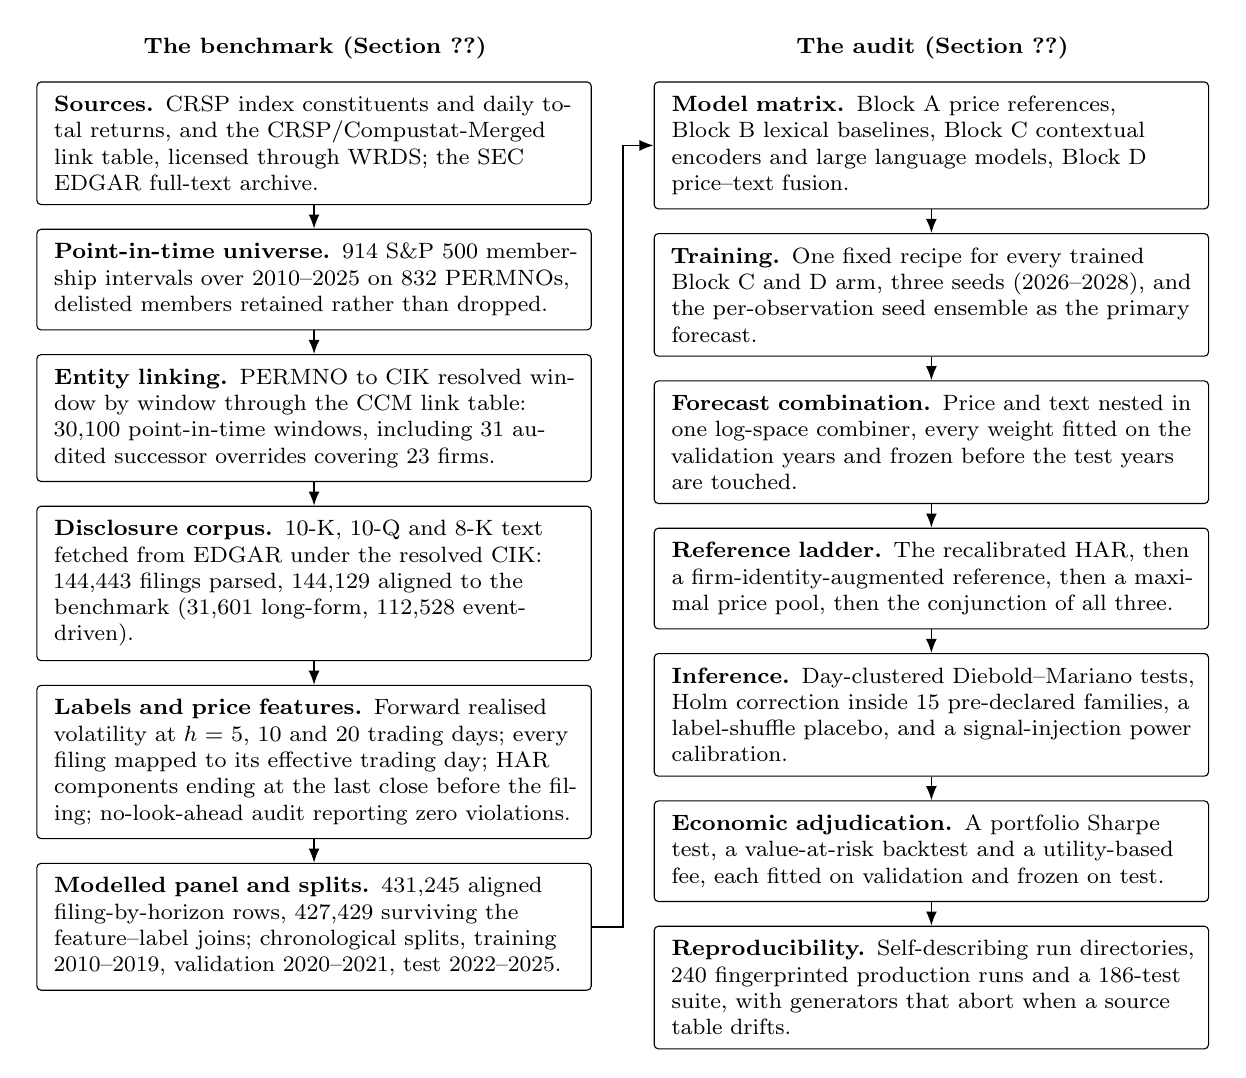
\begin{tikzpicture}[
    font=\footnotesize,
    box/.style={draw, rounded corners=1.5pt, align=left, text width=66mm,
                inner xsep=2.2mm, inner ysep=1.8mm},
    head/.style={align=center, text width=70.4mm, font=\footnotesize\bfseries},
    flow/.style={draw, -{Latex[length=1.8mm,width=1.4mm]}, semithick}]

  \node[head, anchor=north] (h1) at (0mm,0mm)
    {The benchmark (Section~\ref{sec:data-sources})};
  \node[box, below=1.6mm of h1] (a1)
    {\textbf{Sources.} CRSP index constituents and daily total returns, and the
     CRSP/Compustat-Merged link table, licensed through WRDS; the SEC EDGAR
     full-text archive.};
  \node[box, below=3mm of a1] (a2)
    {\textbf{Point-in-time universe.} 914 S\&P~500 membership intervals over
     2010--2025 on 832 PERMNOs, delisted members retained rather than
     dropped.}; % src: crsp_restricted/membership_intervals.csv (914 intervals, 832 PERMNOs)
  \node[box, below=3mm of a2] (a3)
    {\textbf{Entity linking.} PERMNO to CIK resolved window by window through
     the CCM link table: 30{,}100 point-in-time windows, including 31 audited
     successor overrides covering 23 firms.}; % src: crsp_restricted/cik_links_pit.csv; release/DATA_CARD.md lines 45-46
  \node[box, below=3mm of a3] (a4)
    {\textbf{Disclosure corpus.} 10-K, 10-Q and 8-K text fetched from EDGAR
     under the resolved CIK: 144{,}443 filings parsed, 144{,}129 aligned to the
     benchmark (31{,}601 long-form, 112{,}528 event-driven).}; % src: frozen 03_dataset.tex; TECHNICAL_SUPPLEMENT.md Table S1
  \node[box, below=3mm of a4] (a5)
    {\textbf{Labels and price features.} Forward realised volatility at
     $h=5$, 10 and 20 trading days; every filing mapped to its effective
     trading day; HAR components ending at the last close before the filing;
     no-look-ahead audit reporting zero violations.}; % src: frozen 03_dataset.tex (horizons; effective trading day; zero violations)
  \node[box, below=3mm of a5] (a6)
    {\textbf{Modelled panel and splits.} 431{,}245 aligned filing-by-horizon
     rows, 427{,}429 surviving the feature--label joins; chronological splits,
     training 2010--2019, validation 2020--2021, test 2022--2025.}; % src: TECHNICAL_SUPPLEMENT.md Table S1; release/split_definition.md

  \node[head, anchor=north] (h2) at (78.4mm,0mm)
    {The audit (Section~\ref{sec:design})};
  \node[box, below=1.6mm of h2] (b1)
    {\textbf{Model matrix.} Block~A price references, Block~B lexical
     baselines, Block~C contextual encoders and large language models,
     Block~D price--text fusion.};
  \node[box, below=3mm of b1] (b2)
    {\textbf{Training.} One fixed recipe for every trained Block~C and~D arm,
     three seeds (2026--2028), and the per-observation seed ensemble as the
     primary forecast.}; % src: frozen 05_protocol.tex; seed_aggregate.md
  \node[box, below=3mm of b2] (b3)
    {\textbf{Forecast combination.} Price and text nested in one log-space
     combiner, every weight fitted on the validation years and frozen before
     the test years are touched.};
  \node[box, below=3mm of b3] (b4)
    {\textbf{Reference ladder.} The recalibrated HAR, then a
     firm-identity-augmented reference, then a maximal price pool, then the
     conjunction of all three.};
  \node[box, below=3mm of b4] (b5)
    {\textbf{Inference.} Day-clustered Diebold--Mariano tests, Holm correction
     inside 15 pre-declared families, a label-shuffle placebo, and a
     signal-injection power calibration.}; % src: results/tables/holm_families.md (15 families); results/tables/signal_injection_power.md
  \node[box, below=3mm of b5] (b6)
    {\textbf{Economic adjudication.} A portfolio Sharpe test, a value-at-risk
     backtest and a utility-based fee, each fitted on validation and frozen on
     test.};
  \node[box, below=3mm of b6] (b7)
    {\textbf{Reproducibility.} Self-describing run directories, 240
     fingerprinted production runs and a 186-test suite, with generators that
     abort when a source table drifts.}; % src: results/tables/config_fingerprints.md (240 runs); writing/dissertation/supporting/REPRODUCIBILITY.md (186 tests)

  \foreach \i/\j in {a1/a2, a2/a3, a3/a4, a4/a5, a5/a6,
                     b1/b2, b2/b3, b3/b4, b4/b5, b5/b6, b6/b7}
    \draw[flow] (\i.south) -- (\j.north);
  \draw[flow] (a6.east) -- ++(4mm,0mm) |- (b1.west);
  \end{tikzpicture}
  \caption[The pipeline behind SP500Vol-Bench and its audit]{The pipeline of
  Chapter~\ref{ch:data}, drawn as a flow. The left column is the benchmark of
  Section~\ref{sec:data-sources}, running from the three sources to the
  modelled panel and its chronological splits. The right column is the audit of
  Section~\ref{sec:design}, running from the model matrix to the
  reproducibility record. Every box states a stage one of those two sections specifies,
  and every count is the one that section reports; nothing is drawn that they
  do not state. The two external portability panels of
  Section~\ref{sec:data-portability} sit outside this pipeline and are not
  drawn. The diagram carries no result. It shows what was run and in what
  order, not what was found.}
  \label{fig:app-pipeline}
\end{figure}


\begin{figure}[tbp]
  \centering
  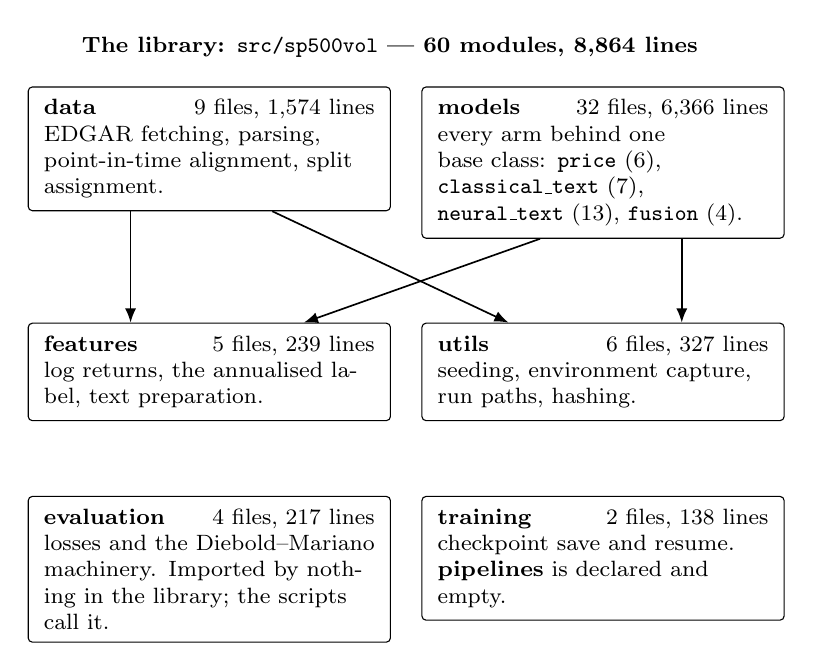
\begin{tikzpicture}[
    font=\footnotesize,
    pkg/.style={draw, rounded corners=1.5pt, align=left, text width=42mm,
                inner xsep=2.0mm, inner ysep=1.6mm},
    grp/.style={draw, dashed, rounded corners=2pt, inner xsep=2.6mm, inner ysep=2.6mm},
    dep/.style={draw, -{Latex[length=1.8mm,width=1.4mm]}, semithick},
    lab/.style={align=center, font=\footnotesize\bfseries}]

  \node[lab] (h) at (0mm,5mm) {The library: \texttt{src/sp500vol} --- 60 modules, 8{,}864 lines};

  \node[pkg, anchor=north west] (data) at (-46mm,0mm)
    {\textbf{data} \hfill 9 files, 1{,}574 lines\\
     EDGAR fetching, parsing, point-in-time alignment, split assignment.};
  \node[pkg, anchor=north west] (models) at (4mm,0mm)
    {\textbf{models} \hfill 32 files, 6{,}366 lines\\
     every arm behind one base class: \texttt{price} (6),
     \texttt{classical\_text} (7), \texttt{neural\_text} (13),
     \texttt{fusion} (4).};

  \node[pkg, anchor=north west] (feat) at (-46mm,-30mm)
    {\textbf{features} \hfill 5 files, 239 lines\\
     log returns, the annualised label, text preparation.};
  \node[pkg, anchor=north west] (utils) at (4mm,-30mm)
    {\textbf{utils} \hfill 6 files, 327 lines\\
     seeding, environment capture, run paths, hashing.};

  \node[pkg, anchor=north west] (eval) at (-46mm,-52mm)
    {\textbf{evaluation} \hfill 4 files, 217 lines\\
     losses and the Diebold--Mariano machinery. Imported by nothing in the
     library; the scripts call it.};
  \node[pkg, anchor=north west] (train) at (4mm,-52mm)
    {\textbf{training} \hfill 2 files, 138 lines\\
     checkpoint save and resume. \textbf{pipelines} is declared and empty.};

  \draw[dep] ([xshift=-10mm]data.south) -- ([xshift=-10mm]feat.north);
  \draw[dep] ([xshift=10mm]models.south) -- ([xshift=10mm]utils.north);
  \draw[dep] ([xshift=8mm]data.south) -- ([xshift=-12mm]utils.north);
  \draw[dep] ([xshift=-8mm]models.south) -- ([xshift=12mm]feat.north);
  \end{tikzpicture}
  \caption[The library, component by component]{The same programme as
  Figure~\ref{fig:app-pipeline}, read as code rather than as a flow. Counts are
  tracked \texttt{.py} files and their lines. Arrows are the only four
  package-level import edges the source contains, derived by parsing every
  import statement rather than inferred from the names. Three non-edges are
  worth as much as the four edges: \texttt{models} imports neither
  \texttt{data} nor \texttt{evaluation}, so an arm cannot reach the corpus or
  its own score while it runs, and nothing under \texttt{src/} imports
  \texttt{scripts/}. Inside \texttt{models} the four arm families each depend
  only on the shared base class, except that \texttt{fusion} and
  \texttt{neural\_text} reuse the text loader in \texttt{classical\_text}. The
  test suite is a sibling of the package, not a part of it: 33 modules
  collecting 186 cases, nine of which exercise \texttt{scripts/} rather than
  the library.} % src: parsed from src/sp500vol/ (60 tracked .py files; 4 package-level import edges: data->features, data->utils, models->features, models->utils); tests/ (33 modules, 184 test functions, two parametrised over two model classes each, so 186 collected)
  \label{fig:app-components}
\end{figure}

\FloatBarrier
\section{Withheld Data, and Why Withholding Is Reproducibility-Neutral}
\label{app:external:withheld}

The CRSP/WRDS licence permits academic research use and bars redistribution of
the raw data and of per-row quantities derived from it \cite{crsp2026data}.
Withheld, therefore, are the daily return series, the realised-volatility labels,
the price features and the per-row model predictions: the last because a
predictions file embeds its label in plain form and is licensed data by
construction. Per-row loss-differential series could in principle be released in
a non-invertible form, carrying differentials alone with no predictions, labels
or features from which a label could be reconstructed. Release would require
written confirmation from the institutional licensing administrator, which the
project did not seek to assume.

The withholding is nonetheless reproducibility-neutral, by design rather than by
assertion. Everything needed to \emph{regenerate} the withheld rows is
released: the universe, the point-in-time links, the split rule, the labelling
code and the pinned configurations. What comes back is not uniform across that
set, and the difference is stated rather than glossed. The CRSP-derived rows
return exactly: the label-parity gate recomputes all 431{,}245 aligned
realised-volatility labels from the raw series on the committed windows and
finds them bitwise identical. The per-row model predictions do not, and this
report turns on that fact elsewhere --- the two executed anonymisation arms were
retained through the registered deviation route precisely because their
regenerations were not bit-identical, one matching 111{,}458 of 117{,}407
predictions and the other none of 333{,}192. A subscription holder therefore
rebuilds the licensed inputs byte-for-byte and the GPU-produced outputs only to
within the nondeterminism this report documents.
% src: results/tables/label_parity.md GATE 1 (n = 431,245, unreconstructed 0, max abs diff 0.000e+00, bitwise exact True); results/tables/anon_arm.md (G1 c6 exact 111,458/117,407; G1 c2 exact 0/333,192)
Everything needed to \emph{audit} the reported claims without a
subscription is released too, because the aggregate evidence tables are summary
statistics carrying no per-row licensed value. Every test statistic, p-value and
correction printed in Chapters~\ref{ch:results} and~\ref{ch:validation} appears
in them. And the one arm whose inputs are entirely public is the prompted model,
which consumes SEC text and emits JSON. It ships nearly complete: prompts, decoding
configuration and 608{,}221 generations, so those outputs can be re-parsed and
re-scored by anyone. The exception is named in the repository rather than left to
be found: the date-only and date-plus-ticker probe generations were not
retained, and their results survive only in the aggregate evidence tables. % src: release/raw_generations/README.md ("The Qwen date-only and date+ticker probe generations were not retained; their results survive in the released aggregate evidence tables.")

\FloatBarrier
\section{Verifying the Numbers in This Report}
\label{app:external:verify}

Three mechanisms make this report checkable. First, the \textbf{source
comments}: every number in the \LaTeX{} sources carries a same-line
\texttt{\% src:} comment naming where it was read from. Of the 868 such comments, 799 name a file the repository carries, so a
marker opening the sources goes from the printed number to the artefact behind
it in one step. Forty-two of those lead with a file in \texttt{release/}, the
public core; the rest lead with results tables, configurations, scripts and
frozen drafting sources. A further 54 name an artefact the licence withholds ---
the per-run predictions and the two CRSP-derived crosswalks --- and one is a
wildcard standing for four configuration files that do ship. The
remaining 14 the census cannot resolve to one file: ten name a cited paper, three
the repository's own commit history and one this report's own chapters. The census is regenerated
from the sources rather than typed, and the build fails if these counts drift.
% src: results/tables/src_comment_census.txt (scripts/analysis/src_comment_census.py)
Every count this report leads
with --- the standalone census, each rung of the ladder, the injection
recoveries and the economic adjudication --- names a file in
\texttt{results/tables/} at its point of use. Any number carried on a secondary basis (a single seed, an
observation-level test, a variance-unit restatement) says so in the prose
beside it. Second, the \textbf{run-artefact contract}: every production run
writes a self-describing directory named
\texttt{\{model\}\_\{dataset\}\_\{disclosure\}\_seed\{seed\}} containing the
fully resolved configuration (\texttt{config.json}), row-level predictions and
per-split metrics. All 240 fingerprinted runs carry those three. An environment
snapshot (\texttt{env.json}) and wall-clock and GPU-hour accounting
(\texttt{cost.json}) are carried by 183 of the 240. The 57 without them are the
38 prompted runs, which train nothing; the six SHAR and HARQ price runs; the six
anonymisation control and mask legs, the four TF--IDF ones being the lineage
whose missing package versions Section~\ref{sec:val-repro} records; and seven
ancillary probe arms. The cut does not fall on training. Of the 178
training-bearing runs 171 carry all five, the seven that do not being those
anonymisation legs and the delta-text probe; and twelve runs that train nothing
at all --- the A1, A3, A4 and A5 price models across the three channels --- carry
them.
% src: release/config_hashes.csv against results/runs/*/ (240 with config.json,
% metrics.json and predictions.parquet; 183 with env.json and cost.json;
% training_sha256_or_blank non-blank in 178, 18 distinct, 171 of them with env.json)
Appendix~\ref{app:fullresults}
reads its grids mechanically from stored artefacts rather than transcribing them
from logs. Third, the \textbf{drift gates}: the fingerprint script re-hashes the
released configurations against the published index, and every table and figure
generator aborts when its source table no longer matches the numbers it
recorded. A stale artefact therefore cannot quietly survive an upstream change.
The recommended order for a marker with the repository to hand is to run
\texttt{config\_fingerprints.py -{}-verify-preimages}, run the test suite, then
pick any claim in Chapter~\ref{ch:results}, read its \texttt{\% src} comment, and
open the named table in \texttt{results/tables/}, where 113 of Chapter~\ref{ch:results}'s 150 source comments lead.

One reconciliation those three mechanisms do not perform for the reader, and
which a careful marker will notice, is worth stating here rather than leaving
to be found. Panel~(c), Figure~\ref{fig:data-membership-b}, stratifies the
long-form test panel by whether the filer later exits, on 822 exiting and
7{,}106 survivor filings. Those sum to 7{,}928, which is 42 fewer than the
7{,}970 long-form test filings of Table~\ref{tab:data-splits}. The two are not
the same denominator: that panel is carried on the superseded early-campaign
convention, as its own caption states, so its row support is that campaign's
rather than the released split's. Nothing else in
the report is computed on the 7{,}928, and no count anywhere is taken as a
share of it.

\FloatBarrier
\section{Project Management, Version Control and Continuous Integration}
\label{app:external:process}

The preceding sections describe what the project produced. This one describes
how it was run, because a reproducibility claim is only as strong as the process
that generated the artefacts behind it, and that process is itself inspectable.
Two things are kept apart throughout. What the process \emph{was} is a matter of
record in the tag list, the workflow definition and the build files; what it
could and could not guarantee is an argument, and it is made explicitly so that
a reader can discount it. The tag list is a property of the version-control
history rather than of any single file, so it is enumerated below in full.

\textbf{Planning: evidence-gated increments, not time-boxed sprints.} The
project had one author and no external client, so no stakeholder existed from
whom requirements had to be elicited. The requirements are the research question
of Section~\ref{sec:intro-aim}, decomposed into the five objectives of
Section~\ref{sec:intro-objectives}, and every deliverable in
Section~\ref{sec:intro-deliverables} answers to one of them. No sprint cadence,
burndown chart or ticket board was kept, and none is reconstructed here: a
borrowed vocabulary applied after the fact would describe this project less
accurately than what actually governed it.

\textbf{Risk: what was not registered, and what actually materialised.} No risk
register was kept either, and none is reconstructed here for the same reason.
What can honestly be given is the other half: the risks that did materialise,
the control that was standing against each when it did, and what the control
cost. Every one is documented elsewhere in this report; gathering them in one
place is what a register would have been for.

\emph{Licence exposure.} The market data are licensed for research and may not
be redistributed, which threatened the release rather than the result. The
control was designed in rather than added: per-row licensed quantities are
withheld and fully regenerable by any licence holder from the released scripts,
and a licence-free variant rebuilds prices from public sources at 72.6, 89.3 and
95.2 per cent coverage of the three splits. The cost is that the public core is
not the panel the results are computed on, which
Section~\ref{sec:data-sources} prices rather than hides.

\emph{Lawful access.} A bulk retrieval from a free public service is a standing
risk to the service and to the project's access. The fetcher declares its
identity, stays inside the published rate limits, and logs every request in a
resumable, retry-safe ledger so that no document is requested twice. The control
was in place before the first bulk pull, not after a failure.

\emph{Silent survivorship bias.} This one materialised. Where a constituent was
acquired or reincorporated, the vendor link could point a historical identifier
at the successor's registrant, under which the original firm filed nothing
during its membership window --- a failure that removes exactly the delisted and
acquired firms whose retention the benchmark's central claim rests on, and
removes them without an error. It was caught by audit rather than by inspection,
and is now held by 31 audited override windows covering 23 firms, a regression
guardrail and dedicated unit tests; the no-look-ahead audit reports zero
violations for those 23 firms in
particular. % src: crsp_restricted/cik_links_pit.csv (30,100 link windows, 31 override windows over 23 firms); frozen 03_dataset.tex (no-look-ahead audit, zero violations including the 23 override firms)

\emph{Loss of the compute estate.} A fleet-scale campaign on rented hardware
carries the risk that the environment disappears before the analysis is
finished, and this one materialised twice. The FinBERT checkpoints were
destroyed in a disk cleanup, which cost the long-form matched-swap replication
one of its three arms, the other two having missed their own reproduction gates
for unrelated reasons; and the earliest run metadata logged no package versions,
which retired three further arms --- the long-form anonymisation exit, the
event-driven anonymisation and the swap TF--IDF arm --- at their gates rather
than allowing them to be rebuilt. The control that was standing --- the reproduction gate
itself, and a written retirement record for every arm that failed one --- did
not save the arms, and was never going to. What it did was make the loss
visible: the retirements are on the record with their thresholds and measured
deviations, and Section~\ref{sec:conc-limitations} states what the missing arms
would have measured. An artefact-retention policy and an environment snapshot on
every run from the first day would have prevented both, and their absence is the
one shortfall in this project's engineering that is hygiene rather than
scope. % src: results/tables/swap_longform_retirement.md (gate, threshold and measured deviation per retired arm); results/runs/*/env.json (183 of 240 carry a snapshot)

The pattern is worth stating because it is not flattering throughout. Two of the
four were designed against in advance and held. One was caught by an audit that
existed for a different purpose. One was not anticipated at all, and the only
control that applied was the one that made the damage countable.

What governed it was the \emph{arm}: a named experimental or audit unit that was
specified in writing, registered under a version-control tag before it ran,
executed, and then either admitted to the evidence base or retired at a stated
gate. Increments closed on evidence rather than on the calendar, and the gates
that closed them are the ones the preceding chapters already document. A derived
arm's statistic may be cited only after a rerun reproduces that arm's committed
predictions to a relative tolerance of $10^{-8}$. A cross-family probe counts as
a live instrument only if it passes the forecaster-health screen, whose two
thresholds read the run's own forecasts and never the contrast under test
(Section~\ref{sec:val-instruments}). And a combination cell is declared genuine
only under the conjunction of clustered significance, Holm correction and the
label-shuffle placebo (Section~\ref{sec:design-inference}). The honest record of
a scheme like this is not its list of successes but its register of failures,
and Section~\ref{sec:val-repro} reports that register in full: the long-form
matched-swap replication lost all three of its arms, and the long-form
anonymisation channel closed with none executed, each exit carrying its gate,
its threshold and its measured deviation. One further registered increment was
retired without ever being scored: the fusion gate's internal weight readout,
whose evidence in this report is behavioural because the direct readout needs a
forward pass that was never run once the fleet was decommissioned. It is one
pass for anyone holding the checkpoints, and it is recorded here rather than
among the open questions of Section~\ref{sec:conc-future} because what the gate
suppressed moves no count. % src: TECHNICAL_SUPPLEMENT.md S19 register
An increment-based plan whose abandoned increments went unreported would be
indistinguishable from no plan at all.

\textbf{What the version-control record shows, and what it cannot.} The
repository carries 26 tags. Twenty-one of them mark pre-registrations in eight
families: seven tags for the long-form matched swap and the entity-anonymisation
arm (\texttt{prereg-ea-v1.0} to \texttt{v1.6}), four for the residual family
audit (\texttt{prereg-rfa-v1.0} to \texttt{v1.3}), three for the earnings-call
panel audit (\texttt{prereg-maec-v1.0} to \texttt{v1.2}), two for the
elicitation-fairness test (\texttt{prereg-ef-v1.0} and \texttt{v1.1}), two for
the tuned challenger arm (\texttt{hpo-prereg-v1.0} and \texttt{v1.1}), and one
each for the mechanism-and-relabelling record (\texttt{prereg-cd-v1.0}), the
licence-free public-price variant (\texttt{prereg-h-v1.0}) and the founding 10-K
corpus audit (\texttt{prereg-kc-v1.0}). % src: git tag -l (26 tags; 21 pre-registration tags in exactly the eight families named, verified 2026-08-04)
The remaining five mark one further pre-test protocol and four writing
milestones. The seven \texttt{prereg-} families correspond one to one with the
seven registered analysis records shipped under \texttt{configs/}. That mapping is
checkable rather than asserted without a copy of the version-control history:
\texttt{release/tag\_manifest.txt} lists every tag beside the commit it pins and
its date, so the eight families can be counted from the repository alone. A second
version number inside a family records an amendment carried by its own tag rather
than a silent edit to the registered file. % src: configs/prereg_*.md (7 records: swap_lf_and_anon, residual_family_audit, maec_audit, elicitation_fairness, mechanism_and_labels, public_variant, kogan_corpus)

A tag is strong evidence of one thing and no evidence of another, and conflating
the two would be an overclaim of exactly the kind this report exists to resist.
It fixes the bytes of the specification the author later claims to have
followed, so any divergence between what was registered and what was reported
can be found mechanically by checking the tag out and comparing. It does not
establish temporal priority. The author holds the repository and the clock
alike, a tag can be moved and a history can be rewritten, so an internal tag
evidences internal consistency and not that the specification preceded the
result. That limitation is why one arm, and only one, carries the external
instrument described at the end of this section.

\textbf{Continuous integration: what runs, and what is only advised.} A workflow
at \texttt{.github/workflows/ci.yml} runs on every push to \texttt{main} and on
every pull request opened against it. Its first job installs the locked
dependency set and runs the test suite on Python 3.11 under the marker
expression \texttt{not slow and not gpu and not network}, so the fast
correctness tests execute on every push while the fleet-scale, GPU-bound and
network-dependent tests are excluded by design. Its second job holds the library and its tests to the
full lint rule set, running \texttt{ruff check} and \texttt{ruff
format -{}-check} over \texttt{src/} and \texttt{tests/}; it checks
\texttt{scripts/} with \texttt{ruff check -{}-select F821,F811,E9}, which is
the errors that would make an analysis script wrong --- an undefined name, a
redefinition, a syntax error --- and not its style, because restyling code
whose outputs are frozen would rewrite files this report depends on for no
gain. It then runs \texttt{mypy} over
\texttt{src/sp500vol/}. % src: .github/workflows/ci.yml (triggers push and pull_request on main; python-version matrix ["3.11"]; pytest marker expression; two ruff lint scopes, one ruff format scope, mypy step)

Two properties of that arrangement need stating plainly, because a flattering
description of them would be the very error this report audits others for.
First, the type-checking step is invoked as
\texttt{mypy src/sp500vol/ \textbar\textbar\ true}, beside a comment recording
that strict typing was deferred, so static type checking here is \emph{advisory
and not enforced}: a type error cannot fail the run. The \texttt{lint} target of
the \texttt{Makefile} runs the same checker without that escape, so the check is
available on demand, but continuous integration does not gate on
it. % src: .github/workflows/ci.yml (mypy step trailing `|| true`, with the in-file comment deferring strict typing); Makefile (lint target runs mypy with no trailing escape)
Second, the project has a single author and its history contains no merge
commits at all, so although the workflow declares a pull-request trigger, no
review by a second party ever took place. What the workflow supplies is a
regression check on one person's pushes, and describing it as a peer-review
process would be false. % src: git log --format='%an' (one author across the whole history); git log --merges (0 merge commits, verified 2026-08-04)

\textbf{Dependency and environment reproducibility.} Three mechanisms operate at
three time scales. \texttt{pyproject.toml} declares the constraints, including a
floor of Python 3.11; \texttt{uv.lock} pins the fully resolved dependency graph
those constraints admit, and the workflow installs through \texttt{uv sync}
against that lock file rather than re-resolving, so the environment that is
checked is the environment that is declared. The \texttt{Makefile} exposes the
routine operations as named targets, among them \texttt{make test},
\texttt{make lint}, \texttt{make format}, \texttt{make data},
\texttt{make train}, \texttt{make tables} and \texttt{make dissertation}, so the
command that produced an artefact is committed rather than
remembered. % src: pyproject.toml (requires-python >= 3.11); uv.lock; Makefile (target list)
The third mechanism is the per-run environment snapshot of
Section~\ref{app:external:verify}, carried by 183 of the 240 runs on the coverage
that section sets out, with the further exception Section~\ref{app:external:regen}
states. The retirement register of
Section~\ref{sec:val-repro} is what that third mechanism looks like when it
fails: the arms whose early snapshots recorded no package versions could not be
rebuilt, and were retired rather than reconstructed by guesswork.

\textbf{The external timestamp, scoped to the one arm that needed it.} One arm
is exposed enough to the priority objection above to warrant an
author-independent instrument.
The tuned challenger of Section~\ref{app:hyperparams:asha} exists to
test whether the fixed training recipe rather than the text produced the null,
and a hyperparameter search is the one arm whose specification, had it been
free to follow the test evaluation, could have been steered towards whichever
conclusion its author preferred. Its pre-registration bundle was therefore
stamped outside the repository.

The stamped object is a single archive,
\texttt{results/prereg/hpo\_prereg\_v1.1.tar}, holding four files and no others:
the arm configuration \texttt{configs/hpo\_arm.yaml}, the design record
\texttt{results/HPO\_ARM\_SPEC.md}, the search harness
\texttt{scripts/experiments/hpo/asha\_hpo.py} and its QLIKE objective
\texttt{scripts/experiments/hpo/qlike\_loss.py}. % src: results/prereg/hpo_prereg_v1.1.tar (tar -tf lists exactly these four members, verified 2026-08-04)
The archive's SHA-256 digest is published beside it in
\texttt{hpo\_prereg\_v1.1.sha256}, and recomputing the digest over the shipped
archive reproduces the published value
exactly. % src: shasum -a 256 -c results/prereg/hpo_prereg_v1.1.sha256 returns OK (digest 2c9a1c9b0b774ef1f330725a39049a57da14e4e7f9a4423e1335fa5f022f5b59, verified 2026-08-04)
An OpenTimestamps proof file sits alongside the archive, and the directory's own
documentation records that the proof was submitted on 14 July 2026 to three
independent calendar servers and anchored in the Bitcoin blockchain, an
attestation that requires no account and discloses no
identity. % src: results/prereg/README.md (timestamp section: submission date, the three named calendars, Bitcoin anchoring)

That last sentence reports what the documentation records, not a check this
report performed. The OpenTimestamps client is absent from the project's
declared and locked environments, so no attestation was verified while this
appendix was written, and the directory carries a smaller, earlier copy of the
proof beside the current one, which is consistent with the upgrade step the same
documentation describes but is not evidence of what either copy now
contains. % src: results/prereg/ (hpo_prereg_v1.1.tar.ots 4,160 bytes dated 2026-07-23; hpo_prereg_v1.1.tar.ots.bak 1,015 bytes dated 2026-07-14; no opentimestamps entry in pyproject.toml or uv.lock, verified 2026-08-04)
The digest is what this report checked. The anchoring is what a reader can check
independently, by installing the client and running \texttt{ots verify} against
the proof file, using nothing beyond that file and a client.

The instrument's scope should not be inflated either. It covers the tuned arm's
bundle and nothing else. The seven registered analysis records carry
version-control tags but no external stamp, so for those seven the available
claim remains internal consistency rather than temporal priority, exactly as set
out above. What the stamp buys, if its attestation verifies, is priority over
the test evaluation of one arm. It does not buy priority over the author's own
thinking, and it says nothing about the audit protocol as a whole. Marking that
boundary is the point of stating it: a report that repeatedly separates a
checked claim from an asserted one cannot afford to assert this one.

\FloatBarrier
\section{The Benchmark Beside the Corpora It Joins}
\label{app:external:benchmarks}

The primary deliverable of this project is a benchmark, which makes its standing
among the resources it joins a claim to evidence rather than to assume.
Table~\ref{tab:app-benchmarks} sets it beside them property by property, and the
properties are the ones an incremental verdict turns on rather than the ones that
flatter a newcomer.

The comparison set is small because the evidence base is small, and its size was
established rather than guessed. The registered audit of the disclosure-text and
volatility literature recorded a census instead of a sample: three corpora carry
that literature. The models built on the earnings-call side all sit on one of the
three by their own documentation, so counting models rather than corpora would
inflate the denominator without adding evidence. % src: results/tables/kogan_corpus_audit.md (census block: three corpora, MDRM/MAEC/Kogan)
Two of the three were audited end to end by this project and the third could not
be obtained. FETILDA joins the table as the long-document evaluation framework
closest to this study's own construction. FinText is treated below the table
rather than tabulated, for the reason given there.

\begin{table}[p]
  \centering
  \caption[The benchmark beside the corpora it joins]{SP500Vol-Bench beside the
  corpora and evaluation frameworks the disclosure-to-volatility literature was
  built on. Two conventions govern the cells, and the distinction between them is
  the point of the table. \textbf{No} records a property this report
  characterises as absent from the design named, on the reading given in
  Section~\ref{sec:bg-text}.
  \textbf{Unknown} records a property this project did not establish for that
  resource from sources it could check; it is not a claim that the resource lacks
  the property, and it is written rather than inferred. Sizes are what this
  project verified, not what each original reports: the MAEC column gives the
  slice actually audited here, while the other two counted columns give
  whole-corpus totals. The table compares documented construction and evaluation
  properties. It is not a ranking of research quality, and nothing in it is a
  test statistic.}
  \label{tab:app-benchmarks}
  \singlespacing\footnotesize
  \setlength{\tabcolsep}{2pt}
  % Narrow measures are set ragged right so that a 1.85 cm column does not stretch
  % its inter-word spacing; \arraybackslash restores \\ as the row terminator.
  \begin{tabular}{@{}>{\raggedright\arraybackslash}p{2.45cm}>{\raggedright\arraybackslash}p{2.85cm}>{\raggedright\arraybackslash}p{2.5cm}>{\raggedright\arraybackslash}p{1.85cm}>{\raggedright\arraybackslash}p{2.35cm}>{\raggedright\arraybackslash}p{2.15cm}@{}}
    \toprule
    Property & SP500Vol-Bench (10-K/10-Q/8-K, 2010--2025) & Kogan 10-K corpus (1996--2006) & FETILDA (10-K) & MAEC (earnings calls) & MDRM (earnings calls) \\
    \midrule
    Size, as verified here
      & 144{,}129 filings; 427{,}429 modelled rows; 803 filing registrants
      & 30{,}474 filings; 7{,}207 registrants
      & unknown
      & audited slice: 672 test rows; 143 call dates; 461 entities
      & unknown; corpus not obtainable \\ % src: release/accession_index.csv (144,129 filings; 803 filing registrants, TECHNICAL_SUPPLEMENT.md Table S1 block b); frozen 03_dataset.tex Table 1 (427,429 modelled rows); results/tables/kogan_corpus_audit.md (30,474 filings, 7,207 unique CIKs); results/tables/maec_audit.md (672 test rows, 143 call dates, 461 entities per horizon)
    \addlinespace[2pt]
    Label and horizon
      & forward realised volatility from daily closes, modelled in logs; $h = 5/10/20$ trading days
      & log volatility over the 12 months after the filing
      & 10-K forward volatility, the Kogan task
      & post-call realised volatility; $h = 3/7/15/30$ days
      & post-call realised volatility \\ % src: frozen 04_methods.tex (horizons h in {5,10,20}); results/tables/kogan_corpus_audit.md (prereg block: logvol.+12 as the target, logvol.-12 as the control); results/tables/maec_audit.md (HAC lag block: h = 3/7/15/30)
    \addlinespace[2pt]
    Survivorship-free point-in-time universe
      & yes: 914 membership intervals, 411 of them closing inside the sample
      & unknown
      & unknown
      & unknown
      & unknown \\ % src: crsp_restricted/membership_intervals.csv (914 intervals; 411 closing inside the sample)
    \addlinespace[2pt]
    Entity linking audited
      & yes: 30{,}100 point-in-time link windows; 31 successor overrides on 23 firms checked against EDGAR
      & unknown
      & unknown
      & unknown
      & unknown \\ % src: crsp_restricted/cik_links_pit.csv (30,100 link windows); release/DATA_CARD.md lines 45-46 (31 override windows covering 23 firms)
    \addlinespace[2pt]
    Recalibrated price reference
      & yes: validation-fitted and frozen, in log space
      & no
      & no
      & no
      & no \\
    \addlinespace[2pt]
    Firm-identity control
      & yes: identity-augmented reference rung, anonymisation, matched-firm swap
      & no
      & no
      & no
      & no \\
    \addlinespace[2pt]
    Inference clustered on the unit sharing the shock
      & yes: day-clustered DM is the test of record
      & no: filings treated as independent
      & no
      & no
      & no \\
    \addlinespace[2pt]
    Power stated as a minimum detectable effect
      & yes: per-cell MDE beside every null; median 0.82 per cent over 69 cells
      & unknown
      & unknown
      & unknown
      & unknown \\ % src: results/tables/signal_injection_power.md (per-cell MDE; median 0.82 per cent, IQR 0.37--1.27). The four non-project cells are Unknown, not No: this project did not establish what any of the four resources reports about its own power, and the caption reserves No for a property Section 2.1.2 characterises as absent.
    \addlinespace[2pt]
    Availability and licence
      & public core released; CRSP market-data rows and the two CRSP-derived crosswalks withheld; public-price variant covers 72.6/89.3/95.2 per cent of train\slash validation\slash test rows
      & public download from the authors' site; the fetch pipeline ships here, the data do not
      & unknown
      & obtainable and used as published; not redistributed here
      & not obtainable: bundled text and audio, no licence, no longer redistributed \\ % src: results/tables/public_variant_cascade.md (72.6/89.3/95.2 per cent coverage); results/tables/kogan_corpus_audit.md (G-K0 provenance: authors' site, data not redistributed; census block: MDRM status)
    \bottomrule
  \end{tabular}
\end{table}

Read across, the table does not say that SP500Vol-Bench is the larger resource,
and on two dimensions it is the smaller. On filer breadth the Kogan corpus spans
7{,}207 registrants against this benchmark's 803, its universe being the
population of 10-K filers where this one is confined to S\&P~500 membership. % src: results/tables/kogan_corpus_audit.md (7,207 unique CIKs); release/accession_index.csv (803 filing registrants, TECHNICAL_SUPPLEMENT.md Table S1 block b)
That confinement was a decision with a price, and Section~\ref{sec:data-sources}
gives the reason. Realised volatility computed from daily closes is noisiest on
thinly traded stocks, so an index restriction buys a label a day-clustered test
can carry. What it forfeits is whatever the small-firm end of the market would
have shown. On modality the benchmark is poorer again, since both earnings-call
resources align speech to text and a filing has no speech to align.

What the table does show is an asymmetry of documentation on exactly the
properties that decide an incremental verdict. Three of them this report
characterises directly for the incumbent designs, and on its reading no
incumbent imposes any: a recalibrated price reference, a firm-identity control,
and inference clustered on the unit that shares the shock. % src: frozen writing/dissertation/supporting/sections/02_related.tex (none of the closest designs imposes a recalibrated price reference, a firm-identity control, or day-clustered inference); results/tables/maec_audit.md (prereg section 8: call-date-clustered inference never provided in the literature)
On point-in-time construction, on entity linking, and on stated power for three
of the four resources, the entry is \emph{unknown}. It is written rather than
filled in. The pattern of unknowns is itself the finding worth stating: these are
properties a reader of the incumbent resources cannot check, and being checkable
is the condition a benchmark contribution is supposed to supply.

The claim the comparison supports is therefore narrow, and it is the claim the
study makes. To the author's knowledge no prior forecast-level evaluation of this
question jointly imposes a survivorship-free point-in-time panel, a recalibrated
reference interval closed by a maximal price pool, day-clustered inference with
Holm correction and placebo gating, and a model spectrum running from word lists
to a prompted large language model. That is a claim about a protocol and the
fixtures released with it, not about corpus size. What makes it checkable is that
the protocol was carried twice to data assembled by others rather than asserted
at home. On the earnings-call corpus the published-convention gain is reproduced
and then absorbed (Section~\ref{app:res-maec}). On the founding study's own 10-K
corpus the published positive is reproduced at the same sign and order of
magnitude, and the cascade then re-prices it
(Section~\ref{sec:val-kogan}). % src: results/tables/maec_audit.md; results/tables/kogan_corpus_audit.md
A protocol that travels to its predecessors and returns the same verdict is
better positioning evidence than a table, and the table is offered as the map
rather than as the argument.

\textbf{FinText, and why it has no column.} FinText forecasts realised volatility
from word embeddings trained on financial newswire and benchmarks against
HAR-family models, which makes it the one design in the survey that cannot be
charged with a weak price baseline \cite{rahimikia2021fintext}. It has no column
because it is a method and a set of embeddings rather than a released volatility
benchmark. Most of the construction properties compared above would have no entry
for it, so the column would be a run of unknowns. Its lesson is the one the table
is built around: a textual claim is won or lost on the baseline, not on the
corpus.

\FloatBarrier
\section{Neural Price Models, and Why the Reference Here Is Linear}
\label{app:external:neural}

Section~\ref{sec:bg-price} takes the price-only reference as far as the HAR
family and its parametric neighbours and stops. A reader is entitled to ask what
lies further out, because every challenger in this study is neural while the
reference each challenger is measured against is not. This section answers in
the only way the evidence permits: it reports what the literature states, and it
is explicit that this project fitted no neural price model and therefore cannot
adjudicate the question itself.

\textbf{What the literature reports.} Recurrent architectures have been applied
to realised-volatility forecasting directly. Bucci \cite{bucci2020neural}
compares feed-forward and recurrent networks, among them long short-term memory
and nonlinear autoregressive specifications, and reports the recurrent models
outperforming the econometric methods in that comparison, with the variants
built to capture long-range dependence doing best. Kim and Won
\cite{kimwon2018lstmgarch} take the hybrid route, feeding the fitted parameters
of several GARCH-type models into a long short-term memory network and reporting
the hybrid ahead of any single GARCH specification on a stock index. Closest to
this project's own question is the comparison of Christensen, Siggaard and
Veliyev \cite{christensen2023mlvol}. They set regularised regressions, regression
trees and neural networks against several HAR specifications, on realised
variance for the constituents of the Dow Jones Industrial Average, and report
machine learning beating the HAR lineage even when the only predictors are the
daily, weekly and monthly realised-variance lags HAR itself uses, with the margin
widening at longer horizons. Their attribution matters as much as the verdict:
the gain comes from greater fitted persistence, which approximates the long
memory of realised variance more closely than a three-lag linear form does.

\textbf{What this study can and cannot say.} It cannot say that HAR beats a
neural price model, because it never fitted one, and no statement anywhere in
this report should be read as a comparison against a neural price baseline that
was tested. Nor can it claim that its reference is the best price forecast
obtainable on this panel. Section~\ref{sec:bg-price} sets the standard that a
credible audit allows the price side its best available representative. This is
the one direction in which the study meets that standard only in part. The rungs
of the reference ladder are recalibration, a firm-identity term and a pool of
linear and parametric specifications, and not one rung is a learned nonlinear
price model.

\textbf{Why a linear reference was nevertheless the right one here.} Three
reasons, in decreasing order of force. The first is protocol parity. HAR-RV is
estimated by ordinary least squares, as is every combination the incremental
instrument fits, so a comparison against it isolates the information source. A
nonlinear learner on the reference side facing a nonlinear learner on the
challenger side would instead confound the information source with estimator
capacity, which is the confusion this design exists to prevent. The
second is that the question is incremental rather than absolute. What the
reference must be is well calibrated and identity-aware, because an uncorrected
reference donates its own miscalibration to the challenger as credit, and the
ladder pays for those two properties explicitly rather than for raw accuracy.
The third is direction, and it is measured rather than argued. Two executed
tests say what a stronger price reference does to the text verdict. The first is
the VIX-augmented re-test of Table~\ref{tab:app-ladder}, which leaves 19 of the 38
re-tested cells standing; the second is the frontier completion of
Section~\ref{app:res-frontier}.
% src: results/tables/vix_control.md (19 of the 38, seed 2026, Holm in 40)
Adding a VIX-augmented HAR and a
measurement-error-corrected HAR to the pool cuts the Holm survivor count from 8
of 69 cells to 3 of 69, on the archived single-seed basis both readings share. % src: results/tables/pool_frontier_audit.md (Holm survivors 8 of 69 under pool5, 3 of 69 under pool7); results/tables/pool_frontier_cascade.csv (genuine_holm, per-cell)
Strengthening the price side has therefore been shown, on this panel, to deepen
the null rather than to relieve it.

\textbf{What the gap costs, and why it cannot now be closed.} An omitted stronger
reference threatens a positive finding, and the finding on text here is a bounded
near-null, so the direction of the threat runs against the residual this study
does report rather than in its favour. Nothing on this evidence suggests a neural
rung would run the other way, though that expectation is an inference from the
frontier test and not a result. Closing the gap would require a new fit, and the
experimental record is frozen: the training fleet is decommissioned, so no rung
can now be added and re-scored under the protocol the rest of the ladder ran.
The gap is recorded as a limitation of scope, of the same class as the arms
Section~\ref{sec:conc-limitations} already lists rather than a new one.

% ============================================================================
% Appendix B ground-up rebuild (W3, 2026-08-02). Expands Section 1.4
% (sec:intro-ethics); must never contradict it. Every number carries a
% same-line evidence comment per the blueprint's verification protocol.
% June draft retired: its "seventeen overrides", "28 runs", "tens of
% GPU-hours" and "single non-significant DM case" are all dead (dossier
% Part 2, Appendices block).
% ============================================================================
\chapter{Legal, Social, Ethical and Professional Issues}
\label{app:ethics}

This appendix records the full assessment summarised in Section~\ref{sec:intro-ethics}, which it expands rather than amends. The project involves no human participants, but obligations do arise from licensed and rate-limited data sources, from reporting forecasting results where misinterpretation has financial consequences, and from the energy the model fleet consumed.

\section{Human Participants and Personal Data}

\textbf{The unit of analysis is the firm.} No participants were recruited, no surveys or interviews conducted, and no personal data collected or processed as research material. Every benchmark row is keyed by a security identifier, a registrant identifier and a trading day; no natural person is a unit of observation, and no statistic in this report is computed for an individual.

Filings do name people (signing officers, directors, executives quoted in event announcements) because statute requires companies to publish those names. They enter the corpus as incidental tokens inside documents already public by legal obligation; the project never extracts, indexes or links them, nor makes any individual the subject of an inference. The anonymisation arm of Section~\ref{sec:res-identity} does the opposite of profiling: it masks every firm name, ticker symbol, executive name, product name and registrant identifier in all 112{,}528 event-driven documents before re-scoring the text; its treatment audit reports that all but one document carries at least one mask and 9.48 per cent of characters are masked on average. % src: results/anon/mask_stats.json (n_docs 112528, docs_with_any_mask_pct 99.99911 = 112,527 of 112,528, mean_mask_char_frac 0.09483); results/tables/anon_arm.md rounds the first of these to "100.0% with >=1 mask"
Identifying language is a confound to be removed, never a variable of interest.

The University's ethical-review procedures attach to research involving human participants, human tissue or personal data; studying corporate entities through public statutory disclosures and licensed market data engages none of them. That conclusion was reached by documented assessment at the project-scoping stage (the ethical-review screening worked through with the supervisor, and its outcome recorded), rather than by assuming that public data is self-exempting.

The instrument that part of the screening was conducted under is the UK General Data Protection Regulation, read with the Data Protection Act 2018, which is what gives the term personal data its meaning here: information relating to an identified or identifiable living individual. The screening put that definition to the research material. What the project collects, stores and analyses is corporate disclosure and licensed market data, organised by firm and by trading day, so nothing in it relates to an individual as a unit of observation. The executive names that statute obliges companies to publish inside those filings were weighed at the same point rather than passed over: they stay as unextracted tokens in documents already public by legal obligation, no individual is made the subject of an inference, and the anonymisation arm masks them in the event-driven copy it re-scores. The outcome recorded was that the University's procedures for research involving personal data are not engaged. That is a screening assessment rather than a compliance determination. It rests on what the material is and on how the project handles it, not on an exemption sought or granted.

\section{Data Licensing and Lawful Access}

\textbf{SEC EDGAR.} The disclosure corpus was retrieved from EDGAR \cite{sec2024edgar}, a free public service whose fair-access policy requires automated clients to identify themselves and to stay within published request-rate limits, so that bulk retrieval does not degrade the service for others. The ingestion pipeline satisfies both by construction rather than by manual restraint: every request declares a user-agent naming the researcher and a contact address; the rate is throttled below the published ceiling of ten requests per second, with exponential back-off on transient errors; and every response is written to a resumable, retry-safe ledger, so no document is fetched twice. That cache later guarantees byte-identical text to every model in the study, % src: results/tables/event_driven_text_cache_validation.txt
so courteous retrieval and reproducible measurement proved to be one engineering decision.

\textbf{CRSP via WRDS.} Daily stock data, index-membership records and the CRSP/Compustat-Merged link table came from the University of Leeds subscription to Wharton Research Data Services \cite{crsp2026data}, under a licence permitting academic research use but barring redistribution of the raw data and of per-row quantities derived from it. That bar determines the shape of the release (Section~\ref{sec:data-public}; Appendix~\ref{app:external}). Withheld are the daily return series, the realised-volatility labels, the price features and the per-row model predictions. Released are the 144{,}129-filing accession index, the split definition, a datasheet, the fingerprints of all 240 production runs, and the aggregate day-clustered evidence tables behind every claim made here. % src: release/DATA_CARD.md; results/tables/config_fingerprints.md
The withheld rows are exactly regenerable from the released scripts by any licence holder. A licence-free variant rebuilds prices from public sources at 72.6, 89.3 and 95.2 per cent coverage of training, validation and test rows; % src: results/tables/public_variant_cascade.md
the attribution wording CRSP and WRDS require is carried in the data card.
Two files that an earlier staging of this release did carry, the membership
intervals and the point-in-time link windows, are withheld. They are per-row
CRSP-derived records: they hold CRSP PERMNOs and CRSP dates, and the link windows
exist precisely to append a CRSP identifier to a series that is not
CRSP's. % src: crsp_restricted/membership_intervals.csv (permno, CRSP dates, source=crsp_wrds_2010_2025); crsp_restricted/cik_links_pit.csv (permno, cik, link windows)
Four clauses reach them. The grant is for internal use, which expressly excludes
further dissemination of the data in electronic form; the subscriber may not
publish or release the data files or the data contained in them outside the
subscribing institution; no derivation from them may be disseminated in
computer-readable form; and CRSP identifiers may not be appended to any other
data series, with any product linking to CRSP data through them requiring a
separate redistribution agreement. The platform's terms of use bar creating
derivative works of the proprietary material, which is defined to include data,
without advance written consent, and carry no exception for identifiers, for
extracts or for research replication. The qualifier those clauses attach --- that
the subscriber's own statement of use may provide otherwise --- does not reach
this case, because redistribution is routed to a separate agreement rather than to
that statement. Withholding costs the study nothing: the ingestion script rebuilds
both files exactly from a CRSP subscription, on the same footing as the withheld
returns and labels, and both remain available to an examiner inside the
institution the subscription covers. % src: CRSP Standard Data Subscription Agreement clauses 1.2, 1.3, 2.1 and 5.3; WRDS Terms of Use section 2; crsp_restricted/README.md; scripts/ingest_wrds.py
What cannot be shared is made rebuildable, and its coverage cost is priced rather
than concealed.

\textbf{External panels.} The portability panels of Section~\ref{sec:data-portability} are public corpora used on their own terms: the Yelp Open Dataset \cite{yelp2024dataset}, in the snapshot taken on 28 July 2026, under its academic licence, which permits non-commercial academic research and bars redistribution, so the project releases the porting scripts and aggregate results rather than the reviews. The MAEC earnings-call corpus \cite{maec2020} is used as published, likewise not redistributed.

\section{Social and Professional Issues}

Financial forecasting research carries a specific social hazard: overstated predictive claims mislead readers into believing a model has economic value it lacks, and lend unearned authority to fragile systems. Every model here is a research artefact built to answer a scientific question --- not a trading system, not investment advice --- and the report says so plainly. The guard against misreading is the report's own arithmetic: no challenger beats the price baseline in any of the 180 standalone comparisons under squared error or volatility-unit QLIKE. % src: results/tables/dm_pairwise_clustered.md (squared error, 0 of 180); results/tables/variance_unit_standalone180.csv (better_qlike_vol_holm 0 of 180; under variance units 7 favour a challenger, every one a GARCH-family price arm)
The residual that does survive the identity-aware reference is reported beside its economic pricing (no significant portfolio gain in any of that arm's six cells, one of eighteen grid-wide). % src: results/tables/firm_identity_ensemble.md; results/tables/portfolio_econ.csv
A small statistical residual therefore cannot be mistaken for a tradable edge.

A second obligation follows from publication bias: a literature tilted towards positive findings rewards searching for a favourable specification and reporting only that. The project was scoped so that a rigorous, reproducible answer counts as success whatever its sign, and the resulting bounded, largely null verdict is reported without softening. No arm was dropped because its results were unwelcome; arms that failed their reproduction gates carry written retirement records rather than disappearing silently; test families were fixed before the statistics were computed; and every null ships the minimum effect it could have detected, so that absence of evidence is never presented as evidence of absence. The reproducibility duty is discharged by the machinery of Section~\ref{sec:design-engineering}: 240 fingerprinted runs (233 distinct digests) with a released re-hashing script, 186 automated tests, and generators that abort when a source table drifts. % src: results/tables/config_fingerprints.md; writing/dissertation/supporting/REPRODUCIBILITY.md

\section{Environmental Cost}

Training and prompting large models consumes energy, and transparent reporting of compute is part of responsible practice. The 144 fixed-recipe production runs of the fine-tuned, frozen-embedding and fusion fleet --- sixteen arms at three seeds by three disclosure channels --- consumed 590.4 GPU-hours on NVIDIA A100-SXM4-40GB hardware (566.7 for Block~C and 23.6 for Block~D), of which the single long-context arm accounts for 254.7, some 43 per cent of that total. % src: results/tables/cost_accuracy.md (basis note: "C/D: 3 seeds x 3 disclosures = 9 runs"; sixteen C/D arm rows)
That figure is a floor rather than the project's whole GPU consumption. The hyper-parameter search ran 63 further trials whose summaries record no runtime, and the anonymisation regenerations retrained on GPU outside the cost record as well; neither is convertible into hours from what was kept. % src: results/hpo/{T1a,T1c,T3d2lf,T4} (63 distinct trial directories, no timing field in summary.json); results/tables/anon_arm.md (c2 GPU retraining under the identical recipe)
That total excludes prompted large-language-model inference, which has no row in the cost record and is reported as excluded rather than silently absorbed. % src: TECHNICAL_SUPPLEMENT.md compute-scope note (cost_accuracy.csv carries no C6/C5x/D4 row)
No facility-level energy or carbon measurement was taken, so no kilowatt-hour or emissions figure is claimed: the GPU-hour total is what the project recorded. Inventing a conversion would violate the evidence discipline the report observes elsewhere.

Several decisions reduced avoidable computation: one-off parsing into a shared text cache every model reads, cached EDGAR responses, validation early stopping with best-epoch restore in place of a fixed epoch budget, and a fingerprinted run store that never repeats a completed run merely to recover a number. One decision deliberately increases cost: three replicate seeds for every fine-tuned arm, roughly tripling the fleet's energy. That is an explicit trade of energy for reliability: 37 of 144 single-seed cells flip the sign of their test statistic across seeds, % src: frozen 05_protocol.tex; results/tables/seed_aggregate.md
so the cheaper campaign would have been the unreliable one. Reporting the total is itself part of the obligation, since it states the cost of reproduction in advance.

\chapter{Full Result Tables}
\label{app:fullresults}


% Figure and table captions in this appendix are set at footnotesize, single
% spaced, as they were when these figures lived in their own appendix; moving
% them must not change how they print.
\captionsetup{font={footnotesize,singlespacing}}
% ============================================================================
% Ground-up rebuild (W3, 2026-08). The June appendix (single-seed, observation-
% level HAC, 57-cell census, "D2 parity" narrative) is discarded in full: every
% table below is rebuilt from the frozen evidence files on the declared primary
% basis, and each carries a "% src:" comment naming the file it is read from.
% ============================================================================

% ----------------------------------------------------------------------------
% Float barriers.  From Section C.14 on, every section is short prose in front
% of one to five near-full-page tables, and the stock float queue could not
% clear them: with \floatpagefraction at 0.95 (figuresetup.tex:38) a float page
% is built only when floats nearly fill one, so tables were held back and pooled
% into a long block at the end of the appendix, the first of them falling ten
% pages after the section that introduces it.  Sixteen \clearpage commands
% survive from that first fix; six sit at a section opening and the other ten
% mid-section, where a run of tables would otherwise straddle a page.
% They are now backed by a \FloatBarrier before every \section in this file,
% added when the dissolved visualisation appendix put 43 figures in here and the
% same queueing began carrying FIGURES across section boundaries -- one landed
% eight pages late, inside a section whose evidence it does not draw.  placeins
% is loaded in config.tex WITHOUT the [section] option: the barriers are written
% out here and in the other appendices, so the page-capped chapters keep the
% stock queue and cannot be pushed past 60 pages by a barrier.
% ----------------------------------------------------------------------------

\FloatBarrier
\section{Scope, Basis and How to Read These Tables}
\label{app:res-basis}

This appendix carries, at full width, the result tables that
Chapter~\ref{ch:results} compresses to headline counts and
Chapter~\ref{ch:validation} draws on selectively. Nothing here is new
evidence: every cell is read mechanically from a committed evidence file,
almost always a table under \texttt{results/tables/} --- the two exceptions are
the HAR-RV reference rows of Tables~\ref{tab:app-standalone-ed}
and~\ref{tab:app-standalone-comb}, read from that run's own
\texttt{metrics.json}, as their comments say --- and each table names its own
evidence file in a provenance comment in the report source directly
beneath its caption. Most numbers in the main text can be traced to a row
here and from there to the artefact that produced it; where a chapter
quantity has no row here, its own provenance comment names the artefact
directly, and a minority of those comments name an internal working
document rather than a released file (Section~\ref{app:external:verify}).

All tables sit on the \emph{primary basis} declared at the opening of
Chapter~\ref{ch:results}, and repeated here because an appendix is read
out of order. The forecast object is the three-seed ensemble (seeds
2026--2028, per-observation mean). The two prompted large-language-model
arms, C6 and D4, are single-pass by construction, so their rows are
identical on either seed basis. Inference is the Diebold--Mariano test
\cite{diebold1995comparing} computed on \emph{day-clustered} loss
differentials: averaged within each trading day, with a
Newey--West correction at lag $h-1$ days and the small-sample adjustment
of \cite{harvey1997testing}. Holm's step-down correction
\cite{holm1979simple} is applied inside each pre-declared family. The
primary loss is QLIKE \cite{patton2011proxies}, evaluated in
\emph{volatility} units on the 69-cell combination grid and in
\emph{variance} units on the standalone leaderboard. Levels are never
compared across those two conventions, and no percentage in one
convention may be set beside a percentage in the other.

Two sign conventions recur and are opposite to one another, which is the
single most common way of misreading these tables. In the
\emph{standalone} tables a \emph{positive} DM statistic means the
challenger named in the row is \emph{worse} than the HAR-RV baseline
\cite{corsi2009har}. In the \emph{combination} tables a \emph{negative}
DM statistic means the text-augmented forecast $f_U$ is \emph{better}
than the reference $f_R$ named in the column group; the accompanying
relative improvement is positive in the same case. Each caption restates
the convention that applies to it.

Two denominators recur. The standalone census has 180 comparisons: 20
challengers carrying committed forecasts on all nine disclosure-by-horizon
panels (long-form, event-driven and combined at $h = 5$, 10 and 20
trading days). Three are price arms and 17 are text or fusion
arms; the latter form the 153-comparison sub-family that the
variance-unit statements are scoped to. The combination grid has 69
cells: 15 long-form and 8 event-driven challengers at three horizons.

Which 20 those are is worth naming, because the model matrix of
Chapter~\ref{ch:data} carries 22 identifiers and a reader cannot
otherwise reconstruct the denominator from it. Nine matrix rows sit
outside the standalone set (\textbf{A1, A6, A7, B1, B3, B4, C5x, C6
and D4}). A2 is the reference every comparison is taken against
rather than a challenger within it. % src: results/tables/dm_pairwise_clustered.csv (20 distinct challenger values x 9 panels = 180 rows; A1, B1, B3, B4 appear zero times)
The nine exclusions are of four kinds, and none of them is a suppressed
result. A1, the naive historical-volatility arm, is carried on the
leaderboard of Table~\ref{tab:app-leaderboard} but was never entered in
the pairwise census. A6 and A7 are scored on the return-matched
subsample and on the point-in-time VIX panel respectively, so their
losses are not computed on the rows the other arms share. Block~B enters
the census through one representative: the classical
representative is fixed as B2 TF--IDF ridge by the generating script's
declared best-of-block rule. That rule is the script's own, not a ranking:
on the best-QLIKE-over-three-horizons ordering this appendix prints, B3
L--M linear sits above B2. % src: scripts/analysis/dm_pairwise.py BASELINE\_MODELS ("Classical / baseline model set (best B = B2\_tfidf\_ridge)"); results/tables/cost_accuracy.csv (qlike_long_form_h20: B3_lm_linear 0.6918 against B2_tfidf_ridge 0.7083)
B1, B3 and B4 therefore carry no census row even
though all three appear in the 69-cell combination grid and, apart from
their absence here, are reported throughout.
And C5x, C6 and D4 are single-seed combination-track arms, excluded on
the same ground that keeps them off the leaderboard.
Expanding the twelve identifiers that remain by their strategy and
embedding variants (C1 at two truncation strategies, C2 at four, C5
and D3 at three embedders each) returns exactly the 20 challengers,
and $20 \times 9 = 180$ comparisons. Three of the 20 are price arms
(A3, A4, A5), leaving the 17 text and fusion arms whose $17 \times 9 =
153$ comparisons carry the variance-unit verdict.
Where a table departs from the primary basis (single seed, observation
level, variance unit, two-way clustered, or a different row support),
the departure is named in the caption and never left to the reader.

A note on row support, because three different supports appear below and
they do not track the reference. The full test panels carry
7{,}951/7{,}933/7{,}902 long-form and 25{,}109/25{,}001/24{,}732
event-driven observations at $h = 5/10/20$. % src: results/tables/dm_pairwise_clustered.md (n_obs)
The merged-grid rows on which the firm-identity and maximal-pool rungs
are evaluated are 7{,}550/7{,}167/7{,}097 and
23{,}855/22{,}785/22{,}318. % src: results/tables/maximal_pool_robustness.csv (n_test); TECHNICAL_SUPPLEMENT.md Table S12
The day counts behind the clustered tests are 809/803/794 long-form
and 996/991/981 event-driven on the full panels, 792/766/765 and
996/991/981 on the merged grid. % src: results/tables/dm_pairwise_clustered.csv (n_days); results/tables/maximal_pool_robustness.csv (n_days)
Percentages computed on one support are not restatements of percentages
computed on another.

Table~\ref{tab:app-denominators} reconciles those row sets in one place, so
that a reader need not hold them in memory. It runs in five groups, set apart by a space:
the standalone census, the combination grid and its ladder, the narrow families
around the 8-K residual, the economic and external panels, and last the two row
supports everything above sits on. It carries no column for \emph{why}
a row set is the size it is, and the paragraphs above therefore remain the only
account of the nine model-matrix rows that sit outside the standalone census.
Three of its entries print as 18 and are not restatements of one another --- the
loss panels of the superior-predictive-ability test, the portfolio cells and the
cells the SHAR substitution touches --- which is the concordance's point rather
than an exception to it. Two units are absent by design: the twenty-comparison
panel of the first two Holm families and the eight-cell arm family of the
fourteenth are correction units rather than denominators, and nothing is stated
on them.

\begin{table}[p]
\centering
\caption[The denominator concordance]{The denominator concordance: the row
sets out of which this report states a count, with what one of its rows is, the
observation support it sits on, and one claim stated on it.}
\label{tab:app-denominators}
\singlespacing\footnotesize
\setlength{\tabcolsep}{3pt}
% src: counts verified against results/tables/ (dm_pairwise_clustered.csv 180 rows;
% control_intersection_ensemble.csv 69 rows and five ladder verdict columns;
% deployable_combiner.csv 75; m1_multiseed.csv 144; m1_stratified.csv 675 rows with
% axis != 'all'; row13_spa_mcs.csv 18 distinct (disclosure, horizon, loss);
% vix_control.csv 40; portfolio_econ.csv 18; utility_value.csv 27 distinct cells;
% var_backtest.csv 36 distinct (disclosure, model, horizon) x 2 nominal levels;
% maec_audit.csv 24 rows at stage row5, alignment primary, over the three text arms).
% Supports read from the n_test column of each of those files.
\begin{tabular}{@{}>{\raggedright\arraybackslash}p{0.15\textwidth}>{\raggedright\arraybackslash}p{0.20\textwidth}>{\raggedright\arraybackslash}p{0.155\textwidth}>{\raggedright\arraybackslash}p{0.335\textwidth}r@{}}
\toprule
Count & One row is & Row support & A claim stated on it & p. \\
\midrule
\addlinespace
180 & one challenger against A2 on one panel & full panels & ``none favours the challenger'' & 28 \\ % src: results/tables/dm_pairwise_clustered.csv (180 rows)
153 & the same, over the 17 text and fusion arms & full panels & ``the 17 text and fusion arms remain 0 of 153 better even there'' & 29 \\ % src: results/tables/variance_unit_standalone180.csv
18 & one (channel, horizon, loss) panel & full panels & ``a consistent $p$ of 1.000 in all 18 panels'' & 50 \\ % src: results/tables/row13_spa_mcs.csv (18 distinct disclosure x horizon x loss)
\addlinespace
69 & one combination cell; 45 long-form, 24 event-driven & full panels; merged grid at the last two rungs & ``the primary basis leaves 38 of 69 cells genuine'' & 31 \\ % src: results/tables/m1_ensemble_primary.csv (n_test 7,951 / 25,109 ...) against firm_identity_ensemble.csv and maximal_pool_robustness.csv (n_test 7,550 / 23,855 ...)
345 & one cell's verdict at one of five rungs ($5 \times 69$) & mixed across the five rungs & ``all 345 cell-level decisions behind the ladder's five 69-cell columns'' & 33 \\ % src: results/tables/control_intersection_ensemble.csv (69 rows; primary_holm, maximal_holm, firm_holm, AND_maximal_firm_holm, AND_full_holm)
38, Holm in 40 & a cell an earlier single-seed screen passed & full panels, seed 2026 & ``leaves 19 of 38 standing'' & 32 \\ % src: results/tables/vix_control.csv (40 rows)
75 & the 69 plus a six-cell C5 extension & full panels & ``the same 75-cell family under expanding weights returns 7 genuine cells'' & 148 \\ % src: results/tables/deployable_combiner.csv (75 rows)
144 & one trained arm at one channel and horizon & full panels, single seed & ``37 of 144 model-by-panel cells flip the sign of their test statistic across seeds'' & 24 \\ % src: results/tables/m1_multiseed.csv (144 rows = 16 models x 3 disclosures x 3 horizons, the combined channel included)
675 & one stratum cell of the increment map & strata of the full panels & ``The placebo is larger in only 38 of the 675 cells'' & 141 \\ % src: results/tables/m1_stratified.csv (675 rows with axis != 'all'; panel (a) draws 567, being 513 of these plus 54 pooled cells)
\addlinespace
12 & C6, two channels, three horizons, two references & full panels (HAR), merged grid (identity) & ``a 12-cell family symmetric around C6 \dots\ it survives all three horizons in both'' & 36 \\ % src: results/tables/residual_symmetric_holm.csv (both n_test supports present)
3 & C6 event-driven, Item 2.02 reference & full event-driven panel & ``The residual retains $+0.21/+0.18/+0.20$ per cent'' & 35 \\ % src: results/tables/itemcode_control.csv
12, Holm in 24 & C6 at one channel, horizon and reference & full panels, split at 2024-07-01 & ``0 of 12 stratified cells'' & 36 \\ % src: results/tables/llm_contamination.md section 3 (24 rows = 12 cells x 2 strata)
6 & the 70B replication, one horizon and reference & full event-driven panel & ``After Holm in its own six-cell family \dots\ only the five-day cell survives'' & 36 \\ % src: results/tables/crossfamily_llama70_ens.csv
6, of 9 readouts & one executed anonymisation arm at one horizon & masked 8-K panel, seed 2026 & ``the pooled median over both executed arms' six vs-HAR cells, $0.51$'' & 38 \\ % src: results/tables/anon_arm.csv (7 rows, 6 of them scored); anon_share_ci.csv (6 per-cell shares, 2 arm medians, 1 pooled median)
\addlinespace
18 & one channel--model--horizon portfolio cell & 159/77/39 and 200/100/50 holding periods & ``a median of $+0.003$ over the 18 cells tested'' & 36 \\ % src: results/tables/portfolio_econ.csv (18 rows; n_periods, the file carrying no observation count)
72 & one (channel, model, horizon) row at one level & merged grid & ``text improves on $f_R$ in 55 of 72 cells'' & 43 \\ % src: results/tables/var_backtest.csv (36 distinct rows x alpha in .01, .05)
27 & one of nine channel--model pairs, one horizon & merged grid & ``the fee is positive in 14 of its own 27 cells'' & 43 \\ % src: results/tables/utility_value.csv (27 distinct disclosure x model x horizon cells)
24 & one MAEC arm, one horizon and reference & 672 rows, 143 call dates & ``0 of the 24 primary-alignment cells'' & 56 \\ % src: results/tables/maec_audit.csv (stage row5, alignment primary, three text arms)
18 & one text arm, SHAR substituted for HAR & return-matched sample & ``changes no verdict in the 18 incremental cells'' & 31 \\ % src: results/tables/stronger_baselines.csv (section m1_incremental)
\addlinespace
7{,}951/\allowbreak 7{,}933/\allowbreak 7{,}902 and 25{,}109/\allowbreak 25{,}001/\allowbreak 24{,}732 & one test observation; combined 33{,}060/\allowbreak 32{,}934/\allowbreak 32{,}634 & census, primary rung, deployable family & ``7{,}951/7{,}933/7{,}902 long-form, 25{,}109/25{,}001/24{,}732 event-driven'' & 28 \\ % src: results/tables/dm_pairwise_clustered.csv (n_obs); m1_ensemble_primary.csv and deployable_combiner.csv (n_test)
7{,}550/\allowbreak 7{,}167/\allowbreak 7{,}097 and 23{,}855/\allowbreak 22{,}785/\allowbreak 22{,}318 & the same, on the pooled references' join & identity and pool rungs, VaR and fee panels & ``on 23{,}855/22{,}785/22{,}318 merged-grid test rows'' & 34 \\ % src: results/tables/maximal_pool_robustness.csv and firm_identity_ensemble.csv (n_test); var_backtest.csv and utility_value.csv carry the same n
\bottomrule
\end{tabular}
\end{table}



The figures interleaved with these tables were drawn for the same evidence and
are placed beside it rather than gathered into a gallery of their own; four of
them, the model spectrum and the efficiency frontier, sit beside the
configuration fields of Appendix~\ref{app:hyperparams} instead. One rule holds
across all of them: each generator carries an evidence gate that aborts the
drawing if the file it reads has drifted from the values the figure was verified
against, so no figure in this report is transcribed by hand. The worked-filing
exhibit of Section~\ref{app:vis-worked} draws nothing and so has no generator to
gate; it names the committed file for every number on the line that states it.

\FloatBarrier
\section{The Fifteen Pre-Declared Holm Families}
\label{app:res-holmfams}

Section~\ref{sec:design-inference} declares that Holm's correction is
applied inside each of 15 pre-declared families and that families are
never pooled, and every survivor count in Chapters~\ref{ch:results}
and~\ref{ch:validation} rests on that declaration. A few corrections in those
chapters are run in blocks that are deliberately \emph{not} among the fifteen,
and each says so where it stands rather than here: the VIX control is corrected
inside its own 40-cell re-test, and the cross-family replication inside the
replication script's own six-cell block. Neither revises a survivor count.
% src: results/tables/holm_families.md lists F1-F15 and neither block is among them; 04_results.tex:181 and :209 carry the two statements
Because it is the
strongest claim this report makes about its own discipline, the
enumeration is carried here in full rather than left to the release
documentation. Table~\ref{tab:app-holm-families} gives, for each family,
what it contains, how large it is, the record that fixed its membership
before the statistics inside it were inspected, and the committed
evidence file that carries its corrected $p$-values.

Four kinds of record appear in the ``declared in'' column, and naming
them separately is more honest than describing all fifteen as
pre-registered. Six families were fixed in a registered analysis record
(the seven \texttt{configs/prereg\_*.md} files inventoried in
Appendix~\ref{app:external}). Five are cited by the version-control tag under
which that record was committed; the sixth, F7, is cited by the record's own
section number instead, its evidence row naming no tag and no bare
\texttt{prereg} tag existing.
% src: results/tables/holm_families.md (F7 declared-in reads "prereg (FACTS 13b)"); git tag -l lists prereg-ea/-rfa/-maec/-ef/-cd/-h/-kc and hpo-prereg, none of them bare
Five were fixed by the protocol itself,
stated in the numbered protocol sections that govern the whole model matrix. Two were fixed by a block
headed \emph{pre-declared Holm families} inside the committed combiner
table, placed above the results it governs and stating in its own heading
that it was written before any result below it was inspected. The
remaining two rest on weaker instruments and are marked as such: one on
the column header of the committed standalone table, and one on the
second-domain plan and its five sanity gates. % src: results/tables/holm_families.md (declared-in column: 5 tag-cited rows F8/F11/F12/F13/F14, plus F7 whose entry reads "prereg (FACTS 13b)" -- a section number, no tag, 5 protocol rows F1/F3-F6, 2 deployable_combiner.md rows F9/F10, 1 table-header row F2, 1 second-domain-plan row F15); results/tables/deployable_combiner.md ("PRE-DECLARED Holm families (declared before any result below was inspected)"); configs/prereg_*.md (7 files)
Every mechanism fixed its family in advance; they differ in how much
external evidence of that fact a reader can inspect, not in whether the
family was pre-declared.

Three conventions travel with the enumeration and are set out here rather
than in the caption. Placebo gates (label shuffle,
$|\mathrm{DM}| < 2$) apply \emph{after} Holm inside the same family, so a
genuine cell requires a negative DM, a Holm-adjusted $p < .05$ and a
clean placebo together. Arms that were never executed, and arms retired
at a reproduction gate, carry no tests and enter no family. And the
not-applicable rule of the anonymisation record governs share estimands
only, never family membership. % src: results/tables/holm_families.md notes (i)-(iii)

Every fixed size in the table is a denominator this report already
prints, and the cross-check is worth stating outright, because a
sixteenth denominator would be a defect. The 180 and 153 of F1 and F2 are
the standalone census and its text-and-fusion subset
(Section~\ref{app:res-basis}); the 69 of F3 to F6, and of each rung of
F12, is the combination grid; the 12 of F7 and the 3 of F8 are the
symmetric residual family and the earnings-window control of
Section~\ref{sec:res-residual}; the 75 of F9 and F10 is that same grid
widened by the six-cell C5 extension (Section~\ref{app:res-deploy}); and
the 24 of F14 is the earnings-call alignment of
Section~\ref{sec:val-external}. % src: results/tables/holm_families.md (size column)
Two rows fix no size of their own, and neither introduces one: F13
inherits the F1 and F3 structures on the public-variant panels, and F15
sets its family per gate.
The correction units named in the Members column of F1, F2 and F14 --- the
20-comparison panel and the eight cells of one MAEC arm --- are not
sixteenth and seventeenth denominators. No count is reported out of
either; they say only how wide the step-down runs, and the counts
themselves are still reported out of the 180, the 153 and the 24. The
distinction matters in one direction only, and it is the unfavourable one:
correcting inside a narrower unit is weaker than correcting across the
whole scope, so these three families are less conservative than their
sizes alone would suggest. The 20-comparison unit is the one every
standalone caption in this appendix already states.

One size does need a word of care, and it is F11. Its 6 is a family
\emph{per executed arm}, three horizons against two references, whereas
the six per-cell identity shares drawn in
Figure~\ref{fig:res-anon-price} panel~(a) are two arms at three horizons.
The two counts sit on the same event-driven rows and count different
objects, so neither is a restatement of the other. % src: results/tables/holm_families.md (F11 members: "3 horizons x 2 references, per executed arm (c6, c2)"); results/tables/anon_arm.csv (6 scored rows: c6 and c2 at h = 5/10/20; b2 carries no cells)

No family is declared and then quietly abandoned. F1 and F2 are reported
in Section~\ref{app:res-standalone}, F3 to F6 in
Sections~\ref{app:res-grid} and~\ref{app:res-ladder}, F7 and F8 in
Section~\ref{sec:res-residual}, F9 and F10 in
Section~\ref{app:res-deploy}, F11 in Section~\ref{sec:res-identity}, F12
in Section~\ref{app:res-rangebased}, F13 in
Section~\ref{app:res-public}, F14 in Section~\ref{app:res-maec} and F15
in Section~\ref{app:res-yelp}.

\begin{table}[htbp]
\centering
\caption[The 15 pre-declared Holm families]{The 15 pre-declared Holm
families, transcribed in full from the release enumeration. Holm's
step-down correction \cite{holm1979simple} is applied \emph{within} each
family and families are never pooled, so no count in this report is
corrected across two of these rows. ``Size'' is the reporting scope; the
``Members'' column names the narrower unit the step-down runs in where
there is one. ``Declared in'' names the record that
fixed the membership before the statistics inside it were inspected;
``carried by'' names the committed evidence file under
\texttt{results/tables/}.}
\label{tab:app-holm-families}
\singlespacing\footnotesize
\setlength{\tabcolsep}{3pt}
% src: results/tables/holm_families.md (all 15 rows verbatim: family, size, members, declared in, carried by; notes (i)-(iii))
\begin{tabular}{@{}l>{\raggedright\arraybackslash}p{0.14\textwidth}l>{\raggedright\arraybackslash}p{0.24\textwidth}>{\raggedright\arraybackslash}p{0.16\textwidth}>{\raggedright\arraybackslash}p{0.20\textwidth}@{}}
\toprule
& Family & Size & Members & Declared in & Carried by \\
\midrule
F1 & Standalone leaderboard & 180 & Challenger against A2 on squared-error DM: models $\times$ disclosures $\times$ horizons; Holm inside each 20-comparison panel & protocol & \texttt{dm\_\allowbreak pairwise\_\allowbreak clustered.csv} \\
F2 & Standalone variance-unit & 153 & The text and fusion subset of F1 under variance-unit QLIKE; a scope, not a unit --- Holm as in F1 & \texttt{variance\_\allowbreak unit\_\allowbreak standalone180.\allowbreak csv} header & \texttt{variance\_\allowbreak unit\_\allowbreak standalone180.\allowbreak csv} \\ % src: that file's holm_qlike_var_clu column carries F2's corrected p-values; F1's carrier, dm_pairwise_clustered.csv, has no variance-unit column at all
\addlinespace
F3 & M1 primary & 69 & Combination cells, volatility unit, seed ensemble & protocol & \texttt{m1\_\allowbreak ensemble\_\allowbreak primary.csv} \\
F4 & M1 variance-unit & 69 & F3 under variance-unit QLIKE & protocol & \texttt{m1\_\allowbreak variance\_\allowbreak unit.csv} \\
F5 & Firm-identity reference & 69 & F3 against the identity-augmented reference; the battery is four specifications, each its own 69-cell family & protocol & \texttt{firm\_\allowbreak identity\_\allowbreak control.csv}, \texttt{firm\_\allowbreak identity\_\allowbreak ensemble.csv} \\
F6 & Maximal pool & 69 & F3 against the five-model price-pool reference & protocol & \texttt{maximal\_\allowbreak reference\_\allowbreak ensemble.md} \\
\addlinespace
F7 & Residual symmetric family & 12 & The pre-declared two-sided 12-cell family for the 8-K residual & \texttt{prereg}, FACTS \S13b & \texttt{omnibus\_\allowbreak m1.md}, \texttt{residual\_\allowbreak symmetric\_\allowbreak holm.md} \\
F8 & Earnings-window control & 3 & C6 event-driven at $h \in \{5, 10, 20\}$ against a firm-identity-plus-Item-2.02 reference & \texttt{prereg-rfa} & \texttt{itemcode\_\allowbreak control.csv} \\
\addlinespace
F9 & Deployable, fixed weights & 75 & Pooled DM per cell, validation-frozen weight scheme & pre-declaration block in \texttt{deployable\_\allowbreak combiner.md} & \texttt{deployable\_\allowbreak combiner.csv} \\
F10 & Deployable, expanding weights & 75 & Pooled DM per cell, expanding weight scheme & as F9 & as F9 \\
\addlinespace
F11 & Anonymisation, per arm & 6 & Three horizons $\times$ two references, within each executed arm (C6, C2) & \texttt{prereg-ea} v1.0/v1.4 & \texttt{anon\_\allowbreak arm.csv} \\
F12 & Range-based Parkinson / Garman--Klass & 69 each & Cascade rungs under the Parkinson and Garman--Klass labels, one family per rung per proxy & \texttt{prereg-cd} v1.0 & \texttt{rangebased\_\allowbreak cascade.csv} \\
F13 & Public-variant panels & as F1/F3 & Panels B and C replicate the F1 and F3 family structures & \texttt{prereg-h} v1.0 & \texttt{public\_\allowbreak variant\_\allowbreak cascade.csv} \\
F14 & MAEC audit & 24 & Four horizons $\times$ three text arms $\times$ two references, clustered; Holm inside each arm's 8 & \texttt{prereg-maec} & \texttt{maec\_\allowbreak audit.md} \\
F15 & Yelp cascade & per gate & Month-clustered DM; label-shuffle placebo primary & second-domain plan, gates G1--G5 & \texttt{yelp\_\allowbreak cascade.md} \\
\bottomrule
\end{tabular}
\end{table}

\FloatBarrier
\section{The Standalone Leaderboard and the 180-Comparison Census}
\label{app:res-standalone}

Table~\ref{tab:app-leaderboard} gives the full long-form standalone
leaderboard: test QLIKE in variance units at each horizon for the 25
models carried on the efficiency-frontier artefact, ordered as that
artefact orders them. A6 sits outside it because it is scored on the
return-matched subsample and A7 on the point-in-time VIX panel, so neither
loss is computed on the rows the other arms share; C5x, C6 and D4 sit
outside it because they are single-seed combination-track arms.
Table~\ref{tab:res-leaderboard} in Chapter~\ref{ch:results} carries the
long-form levels of three of those five, A6, C6 and D4. A7 and C5x carry
no levelled leaderboard row anywhere in the report; their results are
reported in the form each was run for instead. A7 enters the price-pool
completeness audit of Section~\ref{app:res-frontier} (as the
\mbox{HAR-X(VIX)} row) and the joint tests of Tables~\ref{tab:app-spa}
and~\ref{tab:app-mcs}, where it is the beating arm in two of the nine
rejected panels; C5x enters the input-parity control of
Table~\ref{tab:app-c5x}. The GPU-hours are in this appendix's own table.
The ordering is by best QLIKE over the three horizons. Three readings matter. First, the
first five places belong to the five price arms, none of which consumes
a single GPU-hour, and the HAR-RV reference sits third
among them at 0.5564/0.4618/0.2970. Second, the fine-tuned
encoders occupy the bottom: C2 FinBERT at truncation reads
1.3428/1.2440/0.7262, roughly twice the reference's loss at the short
horizons, and no C-block arm reaches the reference at any horizon.
Third, the frozen 7--8B embedding arms (C5) and the price-plus-embedding
fusions (D3) close most of that gap at a fraction of the fine-tuning
cost: D3 with gte-Qwen2 reaches 0.3270 for 0.20 GPU-hours against
C4 Longformer's 0.6051 for 254.72. None of them beats the
reference either. Reading more of the document, and spending twenty
times the compute to do it, moves the text arm without moving it to the
reference.
The event-driven and combined panels carry the same ordering, tabulated in
Section~\ref{app:res-standalone-other}, and the leaderboard is tested jointly
against the objection that its best row was selected after the fact in
Section~\ref{app:res-spamcs}.

\begin{table}[htbp]
\centering
\caption[Full standalone leaderboard, long-form panel]{Full standalone
leaderboard: test QLIKE in \emph{variance units} on the long-form panel,
with total and per-run GPU-hours. C- and D-block rows are the mean over
the three training seeds of each run's test QLIKE (a seed-mean of
per-seed metrics, not the QLIKE of the seed-ensemble forecast: an
off-basis quantity, tagged). A- and B-block rows are seed-invariant and
were run on CPU, reported at $\sim$0 GPU-hours. Lower is better; the A2
HAR-RV reference is the row every DM test in
Table~\ref{tab:app-dm180} is taken against.}
\label{tab:app-leaderboard}
\singlespacing\small
\setlength{\tabcolsep}{4pt}
% src: results/tables/cost_accuracy.md (all QLIKE levels and GPU-hours; ranks as committed)
\begin{tabular}{@{}rllrrrrr@{}}
\toprule
Rank & Model & Block & $h{=}5$ & $h{=}10$ & $h{=}20$ & GPU-h & GPU-h/run \\
\midrule
1  & A3 GARCH            & A & 0.4829 & 0.3750 & 0.2686 & 0.00   & 0.000 \\
2  & A5 ARIMA            & A & 0.5317 & 0.4067 & 0.2732 & 0.00   & 0.000 \\
3  & A2 HAR-RV \emph{(reference)} & A & 0.5564 & 0.4618 & 0.2970 & 0.00 & 0.000 \\
4  & A4 EGARCH           & A & 0.4631 & 0.3541 & 0.3180 & 0.00   & 0.000 \\
5  & A1 Historical vol.  & A & 1.1458 & 0.5600 & 0.3219 & 0.00   & 0.000 \\
6  & D3 price+gte-Qwen2  & D & 0.6698 & 0.5321 & 0.3270 & 0.20   & 0.022 \\
7  & D3 price+E5-Mistral & D & 0.7127 & 0.5688 & 0.3400 & 0.21   & 0.023 \\
8  & D3 price+Qwen3      & D & 0.7486 & 0.6232 & 0.3594 & 0.20   & 0.023 \\
9  & C5 gte-Qwen2        & C & 0.6538 & 0.5714 & 0.3916 & 5.72   & 0.635 \\
10 & C5 Qwen3-emb.       & C & 0.6866 & 0.6045 & 0.3940 & 4.44   & 0.494 \\
11 & D1 Concat-MLP       & D & 0.6408 & 0.6445 & 0.4374 & 11.43  & 1.270 \\
12 & C5 E5-Mistral       & C & 0.8467 & 0.6480 & 0.4375 & 8.94   & 0.993 \\
13 & D2 Gated fusion     & D & 0.7964 & 0.6022 & 0.4410 & 11.60  & 1.288 \\
14 & C2 FinBERT (S2)     & C & 1.4870 & 1.1952 & 0.5720 & 71.27  & 7.919 \\
15 & C2 FinBERT (S4)     & C & 1.4320 & 1.0943 & 0.6032 & 62.43  & 6.936 \\
16 & C4 Longformer (S5)  & C & 1.2351 & 1.0637 & 0.6051 & 254.72 & 28.302 \\
17 & C2 FinBERT (S3)     & C & 1.2430 & 1.2546 & 0.6731 & 67.80  & 7.533 \\
18 & C1 BERT (S2)        & C & 1.4557 & 1.0372 & 0.6905 & 51.73  & 5.748 \\
19 & B3 L--M linear      & B & 1.2937 & 1.0649 & 0.6918 & 0.00   & 0.000 \\
20 & C1 BERT (S1)        & C & 1.6444 & 1.1968 & 0.6995 & 13.71  & 1.523 \\
21 & B2 TF--IDF ridge    & B & 1.2371 & 1.0522 & 0.7083 & 0.00   & 0.000 \\
22 & B4 L--M features    & B & 1.4166 & 1.1223 & 0.7231 & 0.00   & 0.000 \\
23 & C2 FinBERT (S1)     & C & 1.3428 & 1.2440 & 0.7262 & 12.65  & 1.406 \\
24 & C3 RoBERTa (S1)     & C & 1.6303 & 1.0863 & 0.7518 & 13.31  & 1.479 \\
25 & B1 BoW ridge        & B & 2.2844 & 1.5916 & 1.0668 & 0.00   & 0.000 \\
\bottomrule
\end{tabular}
\end{table}

Table~\ref{tab:app-dm180} is the census itself: all 180 day-clustered DM
statistics against HAR-RV as a standalone forecaster, one row per
challenger and one column per disclosure-by-horizon panel. Every one of
the 180 statistics is positive. That is a stronger statement than the
significance count, because it means no comparison anywhere in the
census carries even a favourable point estimate for a test to
adjudicate. In addition, 155 of the 180 are significantly worse after
Holm correction within each 20-challenger panel. The gradient across the
table is informative in its own right: the fusion arms that carry the
price signal inside them (D1--D3) produce the smallest statistics and
account for 21 of the 25 non-significant cells. The pure
encoders sit between $+2.86$ and $+9.57$ throughout. A fusion arm
failing to be separated from the reference is not a text result, and the
table is laid out so that the two cannot be confused.

\begin{table}[p]
\centering
\caption[The 180-comparison standalone census]{The full standalone
census: day-clustered Diebold--Mariano statistics on squared forecast
error against A2 HAR-RV as a standalone forecaster, seed-ensemble
forecasts, all 20 challengers on all nine disclosure-by-horizon panels.
\emph{Positive means the challenger is worse than the baseline.} An
asterisk marks Holm significance within that panel's 20-comparison
family. All 180 statistics are positive; 155 are Holm-significantly
worse. Panel supports: long-form 7{,}951/7{,}933/7{,}902 observations
over 809/803/794 days, event-driven 25{,}109/25{,}001/24{,}732 over
996/991/981, combined 33{,}060/32{,}934/32{,}634 over 996/991/981.}
\label{tab:app-dm180}
\singlespacing\footnotesize
\setlength{\tabcolsep}{3.5pt}
% src: results/tables/variance_unit_standalone180.csv (dm_se_clu, worse_se_holm); cross-checked against results/tables/dm_pairwise_clustered.csv
\begin{tabular}{@{}lrrrrrrrrr@{}}
\toprule
& \multicolumn{3}{c}{Long-form (10-K/Q)} & \multicolumn{3}{c}{Event-driven (8-K)} & \multicolumn{3}{c}{Combined} \\
\cmidrule(lr){2-4}\cmidrule(lr){5-7}\cmidrule(lr){8-10}
Challenger & $h{=}5$ & $h{=}10$ & $h{=}20$ & $h{=}5$ & $h{=}10$ & $h{=}20$ & $h{=}5$ & $h{=}10$ & $h{=}20$ \\
\midrule
A3 GARCH               & $+5.22$* & $+4.73$* & $+4.27$* & $+4.33$* & $+3.37$* & $+2.58$\phantom{*} & $+6.08$* & $+4.78$* & $+3.49$* \\
A4 EGARCH              & $+2.74$* & $+2.39$\phantom{*} & $+3.61$* & $+5.75$* & $+5.08$* & $+3.96$* & $+6.26$* & $+5.46$* & $+4.18$* \\
A5 ARIMA               & $+5.84$* & $+4.21$* & $+3.10$* & $+5.48$* & $+3.75$* & $+2.20$\phantom{*} & $+6.17$* & $+4.12$* & $+2.27$\phantom{*} \\
\addlinespace
B2 TF--IDF ridge       & $+6.35$* & $+4.92$* & $+3.62$* & $+9.54$* & $+8.18$* & $+7.01$* & $+9.47$* & $+8.06$* & $+6.64$* \\
C1 BERT (S1)           & $+7.64$* & $+4.66$* & $+3.66$* & $+8.13$* & $+6.83$* & $+5.28$* & $+9.19$* & $+6.05$* & $+6.12$* \\
C1 BERT (S2)           & $+7.21$* & $+4.42$* & $+3.46$* & $+8.71$* & $+7.31$* & $+5.82$* & $+9.56$* & $+6.85$* & $+5.67$* \\
C2 FinBERT (S1)        & $+6.68$* & $+5.53$* & $+3.32$* & $+7.18$* & $+7.07$* & $+5.34$* & $+8.19$* & $+5.97$* & $+5.25$* \\
C2 FinBERT (S2)        & $+7.63$* & $+5.11$* & $+3.12$* & $+8.54$* & $+7.29$* & $+5.14$* & $+8.73$* & $+6.89$* & $+5.50$* \\
C2 FinBERT (S3)        & $+6.68$* & $+5.50$* & $+3.41$* & $+7.43$* & $+6.00$* & $+5.04$* & $+8.89$* & $+6.50$* & $+5.35$* \\
C2 FinBERT (S4)        & $+7.07$* & $+4.89$* & $+2.86$* & $+8.08$* & $+6.29$* & $+6.06$* & $+9.49$* & $+6.65$* & $+4.98$* \\
C3 RoBERTa (S1)        & $+7.68$* & $+5.61$* & $+3.87$* & $+7.47$* & $+7.11$* & $+5.84$* & $+8.66$* & $+7.54$* & $+5.88$* \\
C4 Longformer (S5)     & $+6.06$* & $+4.56$* & $+2.92$* & $+7.87$* & $+6.51$* & $+5.73$* & $+9.01$* & $+6.80$* & $+5.36$* \\
C5 E5-Mistral          & $+5.24$* & $+6.96$* & $+6.76$* & $+8.38$* & $+7.44$* & $+6.62$* & $+9.07$* & $+7.70$* & $+6.52$* \\
C5 gte-Qwen2           & $+6.71$* & $+7.31$* & $+6.67$* & $+9.57$* & $+9.02$* & $+8.77$* & $+8.92$* & $+7.79$* & $+6.61$* \\
C5 Qwen3-emb.          & $+5.92$* & $+7.08$* & $+6.79$* & $+9.20$* & $+8.66$* & $+7.70$* & $+8.78$* & $+7.63$* & $+6.38$* \\
D1 Concat-MLP          & $+1.61$\phantom{*} & $+2.62$\phantom{*} & $+2.44$\phantom{*} & $+6.98$* & $+6.43$* & $+5.07$* & $+6.85$* & $+4.74$* & $+3.92$* \\
D2 Gated fusion        & $+3.53$* & $+1.86$\phantom{*} & $+2.03$\phantom{*} & $+6.47$* & $+5.73$* & $+4.30$* & $+7.22$* & $+5.34$* & $+5.65$* \\
D3 price+E5-Mistral    & $+3.19$* & $+1.96$\phantom{*} & $+0.63$\phantom{*} & $+3.92$* & $+2.51$* & $+1.83$\phantom{*} & $+4.07$* & $+2.14$\phantom{*} & $+2.42$\phantom{*} \\
D3 price+gte-Qwen2     & $+1.91$\phantom{*} & $+0.77$\phantom{*} & $+0.24$\phantom{*} & $+2.24$* & $+2.11$* & $+1.16$\phantom{*} & $+2.69$* & $+0.99$\phantom{*} & $+0.24$\phantom{*} \\
D3 price+Qwen3         & $+3.81$* & $+2.62$\phantom{*} & $+1.26$\phantom{*} & $+3.73$* & $+2.52$* & $+1.80$\phantom{*} & $+3.80$* & $+1.90$\phantom{*} & $+1.93$\phantom{*} \\
\bottomrule
\end{tabular}
\end{table}

Table~\ref{tab:app-census} re-adjudicates those same 180 comparisons
(the same forecasts, the same rows) under three loss conventions and
three error structures. It gives the 153-comparison text-and-fusion
sub-family alongside the full census in the four rows that carry it; the
superseded observation-level row and the two-way row print a dash there, that
decomposition never having been computed on either. The one convention
that produces winners is the variance-unit restatement, and all seven
winners are price arms: A3 GARCH in six cells and A4 EGARCH at long-form
$h{=}5$. Under that convention the text and fusion arms are not merely
0 of 153 better; they are 153 of 153 significantly \emph{worse}, the
harshest verdict any convention returns on them. Moving from
observation-level HAC to day clustering and then to two-way firm-by-day
clustering \cite{cameron2011twoway} costs the study evidence at every
step: the significantly-worse count falls 174, 155, 152 and the
median absolute statistic falls 15.44, 5.70, 4.86. All three are
therefore printed rather than the primary alone.

\begin{table}[htbp]
\centering
\caption[The 180-comparison census under three losses and three error
structures]{The standalone census re-adjudicated. Panel (a) holds the
error structure at the day-clustered primary and changes the loss; panel
(b) holds the loss at squared error and changes the error structure.
Identical forecasts, rows and Holm families throughout; only the named
axis moves. ``DM $<0$'' counts comparisons carrying a favourable point
estimate before any test; ``better'' and ``worse'' are Holm-corrected
within each 20-challenger panel. ``med.'' is the median absolute DM
statistic over the 180 comparisons. The text/fusion sub-family is the 17
non-price challengers over the nine panels; a dash means the source file
does not carry that decomposition.}
\label{tab:app-census}
\singlespacing\small
\setlength{\tabcolsep}{4pt}
% src: results/tables/variance_unit_standalone180.csv (all counts re-derived 2026-08-02); median |DM| from TECHNICAL_SUPPLEMENT.md Table S3(a); obs-level and two-way counts from results/tables/dm_pairwise_clustered.md and results/tables/twoway_cluster.md
\begin{tabular}{@{}lrrrrrr@{}}
\toprule
& \multicolumn{4}{c}{All 180 comparisons} & \multicolumn{2}{c}{Text/fusion (153)} \\
\cmidrule(lr){2-5}\cmidrule(lr){6-7}
Convention & DM $<0$ & better & worse & med. & better & worse \\
\midrule
\multicolumn{7}{@{}l}{\emph{(a) Day-clustered inference; loss convention varied}} \\
Squared error (primary) & 0  & 0 & 155 & 5.70  & 0 & 132 \\
QLIKE, volatility units & 1  & 0 & 161 & ---   & 0 & 146 \\
QLIKE, variance units   & 14 & 7 & 153 & ---   & 0 & 153 \\
\midrule
\multicolumn{7}{@{}l}{\emph{(b) Squared error; error structure varied}} \\
Observation-level HAC \emph{(superseded)} & 0 & 0 & 174 & 15.44 & --- & --- \\
Day-clustered, lag $h-1$ days             & 0 & 0 & 155 & 5.70  & 0 & 132 \\
Two-way firm $\times$ day                 & 0 & 0 & 152 & 4.86  & --- & --- \\
\bottomrule
\end{tabular}
\end{table}

\FloatBarrier
\section{The 69-Cell Combination Grid}
\label{app:res-grid}

Tables~\ref{tab:app-grid-ed} and~\ref{tab:app-grid-lf} are the
combination grid cell by cell: the 24 event-driven and 45 long-form
cells at the primary rung. Each carries its relative QLIKE improvement over
the recalibrated HAR reference, its day-clustered DM statistic, its
Holm-adjusted $p$ within the 69-cell family, its label-shuffle placebo
statistic and the genuine verdict that requires all three. The right-hand
column groups then carry the same cell's increment over the fitted
maximal price pool and over the firm-identity reference, with their own
Holm verdicts. Read together the two tables reproduce every count in
Chapter~\ref{ch:results}: 46 cells at raw $p<.05$, 38 genuine, 9
surviving the pool, 8 surviving firm identity, and no row anywhere
carrying a Y in both of the last two column pairs.
Every weight behind these cells is fitted once on the validation block and
frozen. Section~\ref{app:res-deploy} reruns the same cells under weights
refitted before each quarter on strictly earlier filings, which is what a
forecaster running the method would have had to do.

Three features of the grid are visible only at this resolution. The
surviving primary-rung increments are not uniformly negligible: they
reach $+5.92\%$ (long-form B2 TF--IDF ridge at $h{=}20$) and the grid
spans $-3.86\%$ to $+5.92\%$. The stronger references are therefore
adjudicating real quantities rather than rounding error. The placebo
column earns its place by not firing: of the 38 cells with a negative DM
statistic and a Holm-adjusted $p$ below .05, none has a label-shuffle
statistic outside the $|\mathrm{DM}|<2$ pass band. The placebo gate
removes no cell that the correction had not already removed: a
null result for that instrument on this grid, reported as such. The two
largest placebo statistics in either table, $-3.17$ at long-form B4 L--M
features $h{=}20$ and $+3.00$ at event-driven D2 gated fusion $h{=}5$,
sit on cells that are already excluded. The first has a negative
increment; the second fails Holm at $p = .988$. And the
seed column matters for interpretation rather than
for arithmetic: 33 of the 69 cells are three-seed ensembles and 36 are
single-seed by construction (the four B-block arms are deterministic
fits and the two prompted arms have no training seed). The ensemble basis is a
statement about the C1--C5 and D1--D3 rows and leaves the rest untouched: the
twelve C6 and D4 cells sit in the C and D blocks and are single-seed too. % src: results/tables/control_intersection_ensemble.csv (45 C/D rows: 33 with n_seeds 3, 12 with n_seeds 1, those twelve being C6_llmtext and D4_llmfused)

\begin{table}[htbp]
\centering
\caption[The 69-cell combination grid: event-driven cells]{The
combination grid, \textbf{event-driven (8-K) channel}, all 24 cells.
Basis: seed-ensemble forecasts, volatility-unit QLIKE, log-space
combiner fitted on validation and frozen on test, day-clustered DM with
Holm inside the 69-cell family. \emph{Negative DM and positive rel.\%
mean text improves on the reference.} $s$ = number of training seeds;
plac.\ = label-shuffle placebo DM (pass band $|$DM$|<2$); G = genuine at
the primary rung (DM $<0$, Holm $<.05$, placebo in band). The last two
column pairs are the same cell's increment over the fitted five-model
price pool and over the firm-identity-augmented reference, each with its
own Holm verdict on the merged-grid support.}
\label{tab:app-grid-ed}
\singlespacing\footnotesize
\setlength{\tabcolsep}{3.5pt}
% src: results/tables/control_intersection_ensemble.csv (all columns); rung counts cross-checked against m1_ensemble_primary.md, maximal_reference_ensemble.md, firm_identity_ensemble.md
\begin{tabular}{@{}lrrrrrrcrcrc@{}}
\toprule
& & & \multicolumn{5}{c}{Primary rung: recalibrated HAR} & \multicolumn{2}{c}{Maximal pool} & \multicolumn{2}{c}{Firm identity} \\
\cmidrule(lr){4-8}\cmidrule(lr){9-10}\cmidrule(lr){11-12}
Model & $h$ & $s$ & rel.\% & DM & Holm $p$ & plac. & G & rel.\% & Holm & rel.\% & Holm \\
\midrule
B1 BoW ridge       &  5 & 1 & $+1.331$ & $-3.35$ & .0252 & $+0.59$ & Y & $+0.312$ & -- & $+0.461$ & Y \\
B1 BoW ridge       & 10 & 1 & $+1.229$ & $-3.25$ & .0332 & $+0.05$ & Y & $-0.157$ & -- & $+0.250$ & Y \\
B1 BoW ridge       & 20 & 1 & $+1.531$ & $-3.10$ & .0489 & $+0.45$ & Y & $-0.267$ & -- & $-0.193$ & -- \\
B2 TF--IDF ridge   &  5 & 1 & $+1.207$ & $-2.76$ & .1237 & $+0.39$ & -- & $+0.147$ & -- & $+0.444$ & -- \\
B2 TF--IDF ridge   & 10 & 1 & $+1.355$ & $-2.97$ & .0681 & $+0.38$ & -- & $-0.058$ & -- & $+0.281$ & Y \\
B2 TF--IDF ridge   & 20 & 1 & $+1.840$ & $-3.11$ & .0489 & $+0.42$ & Y & $-0.127$ & -- & $-0.045$ & -- \\
B3 L--M linear     &  5 & 1 & $+0.248$ & $-2.43$ & .2730 & $+0.01$ & -- & $+0.161$ & -- & $+0.110$ & -- \\
B3 L--M linear     & 10 & 1 & $+0.200$ & $-1.23$ & 1.0000 & $+0.16$ & -- & $+0.087$ & -- & $+0.108$ & -- \\
B3 L--M linear     & 20 & 1 & $+0.260$ & $-1.12$ & 1.0000 & $+0.84$ & -- & $+0.094$ & -- & $+0.170$ & -- \\
B4 L--M feat.      &  5 & 1 & $+0.184$ & $-0.99$ & 1.0000 & $+0.46$ & -- & $+0.195$ & -- & $+0.218$ & -- \\
B4 L--M feat.      & 10 & 1 & $+0.082$ & $-2.10$ & .6041 & $-0.05$ & -- & $+0.084$ & -- & $+0.130$ & -- \\
B4 L--M feat.      & 20 & 1 & $+0.247$ & $-2.01$ & .6569 & $+0.47$ & -- & $+0.086$ & -- & $+0.110$ & -- \\
C2 FinBERT (S1)    &  5 & 3 & $+2.572$ & $-5.92$ & $<$.0001 & $-1.72$ & Y & $+0.768$ & -- & $-0.061$ & -- \\
C2 FinBERT (S1)    & 10 & 3 & $+2.416$ & $-5.68$ & $<$.0001 & $+0.96$ & Y & $+0.084$ & -- & $-0.665$ & -- \\
C2 FinBERT (S1)    & 20 & 3 & $+1.578$ & $-1.94$ & .6569 & $+0.33$ & -- & $-1.594$ & -- & $-0.613$ & -- \\
C6 prompted LLM    &  5 & 1 & $+1.214$ & $-5.04$ & $<$.0001 & $+0.10$ & Y & $+0.398$ & -- & $+0.518$ & Y \\
C6 prompted LLM    & 10 & 1 & $+0.998$ & $-3.76$ & .0065 & $+0.95$ & Y & $+0.121$ & -- & $+0.244$ & Y \\
C6 prompted LLM    & 20 & 1 & $+0.658$ & $-1.98$ & .6569 & $+1.11$ & -- & $+0.086$ & -- & $+0.215$ & Y \\
D2 Gated fusion    &  5 & 3 & $+0.559$ & $-1.70$ & .9875 & $+3.00$ & -- & $+0.297$ & -- & $+0.226$ & -- \\
D2 Gated fusion    & 10 & 3 & $+0.177$ & $-0.42$ & 1.0000 & $-0.20$ & -- & $-0.017$ & -- & $+0.050$ & -- \\
D2 Gated fusion    & 20 & 3 & $-2.764$ & $+3.55$ & .0139 & $-0.44$ & -- & $-2.486$ & -- & $-7.992$ & -- \\
D4 price+C6        &  5 & 1 & $-0.013$ & $+3.37$ & .0241 & $+1.58$ & -- & $+0.114$ & -- & $-0.072$ & -- \\
D4 price+C6        & 10 & 1 & $-0.008$ & $+0.66$ & 1.0000 & $-0.08$ & -- & $-0.030$ & -- & $-0.021$ & -- \\
D4 price+C6        & 20 & 1 & $-0.355$ & $+4.69$ & .0001 & $-0.19$ & -- & $-0.243$ & -- & $-0.251$ & -- \\
\midrule
\multicolumn{12}{@{}l}{\emph{Event-driven subtotals: 8 genuine of 24; 0 surviving the maximal pool; 6 surviving firm identity.}} \\
\bottomrule
\end{tabular}
\end{table}

\begin{table}[p]
\centering
\caption[The 69-cell combination grid: long-form cells]{The combination
grid, \textbf{long-form (10-K/Q) channel}, all 45 cells. Columns,
conventions and sign rules exactly as in Table~\ref{tab:app-grid-ed}.
One pool survivor carries an increment too small to print at three
decimals: long-form D1 Concat-MLP at $h{=}20$ reads $+0.001\%$ over the
pool, which is a Holm survivor on an increment of essentially zero and
is shown rather than rounded away.}
\label{tab:app-grid-lf}
\singlespacing\footnotesize
\setlength{\tabcolsep}{3.5pt}
% src: results/tables/control_intersection_ensemble.csv (all columns)
\begin{tabular}{@{}lrrrrrrcrcrc@{}}
\toprule
& & & \multicolumn{5}{c}{Primary rung: recalibrated HAR} & \multicolumn{2}{c}{Maximal pool} & \multicolumn{2}{c}{Firm identity} \\
\cmidrule(lr){4-8}\cmidrule(lr){9-10}\cmidrule(lr){11-12}
Model & $h$ & $s$ & rel.\% & DM & Holm $p$ & plac. & G & rel.\% & Holm & rel.\% & Holm \\
\midrule
B1 BoW ridge       &  5 & 1 & $+1.645$ & $-3.83$ & .0050 & $+0.43$ & Y & $+0.870$ & -- & $-0.138$ & -- \\
B1 BoW ridge       & 10 & 1 & $+1.443$ & $-4.15$ & .0015 & $+0.39$ & Y & $+0.506$ & -- & $-2.720$ & -- \\
B1 BoW ridge       & 20 & 1 & $+2.986$ & $-5.45$ & $<$.0001 & $-0.25$ & Y & $+1.608$ & -- & $-4.985$ & -- \\
B2 TF--IDF ridge   &  5 & 1 & $+3.331$ & $-5.39$ & $<$.0001 & $+0.51$ & Y & $+1.672$ & Y & $-0.615$ & -- \\
B2 TF--IDF ridge   & 10 & 1 & $+3.482$ & $-8.89$ & $<$.0001 & $+0.33$ & Y & $+1.952$ & Y & $-3.892$ & -- \\
B2 TF--IDF ridge   & 20 & 1 & $+5.920$ & $-9.04$ & $<$.0001 & $+0.30$ & Y & $+4.013$ & Y & $-8.089$ & -- \\
B3 L--M linear     &  5 & 1 & $+0.495$ & $-2.58$ & .1894 & $+0.59$ & -- & $-0.221$ & -- & $+0.207$ & -- \\
B3 L--M linear     & 10 & 1 & $+1.794$ & $-4.62$ & .0002 & $+0.27$ & Y & $+0.641$ & -- & $+0.261$ & Y \\
B3 L--M linear     & 20 & 1 & $+3.485$ & $-4.69$ & .0001 & $-1.26$ & Y & $+1.927$ & -- & $-0.017$ & -- \\
B4 L--M feat.      &  5 & 1 & $+0.113$ & $+1.02$ & 1.0000 & $+0.43$ & -- & $+0.023$ & -- & $-0.139$ & -- \\
B4 L--M feat.      & 10 & 1 & $-0.922$ & $+3.32$ & .0276 & $-1.69$ & -- & $-0.729$ & -- & $-2.767$ & -- \\
B4 L--M feat.      & 20 & 1 & $-1.920$ & $+3.38$ & .0241 & $-3.17$ & -- & $-1.554$ & -- & $-7.133$ & -- \\
C1 BERT (S1)       &  5 & 3 & $+3.420$ & $-3.25$ & .0332 & $-0.03$ & Y & $+1.088$ & -- & $+1.376$ & -- \\
C1 BERT (S1)       & 10 & 3 & $-0.849$ & $+3.06$ & .0533 & $-1.02$ & -- & $-0.112$ & -- & $-4.751$ & -- \\
C1 BERT (S1)       & 20 & 3 & $+2.702$ & $-6.96$ & $<$.0001 & $+0.39$ & Y & $+0.896$ & -- & $-6.488$ & -- \\
C2 FinBERT (S1)    &  5 & 3 & $+1.898$ & $-4.53$ & .0003 & $-0.72$ & Y & $+0.626$ & -- & $-0.268$ & -- \\
C2 FinBERT (S1)    & 10 & 3 & $+2.616$ & $-6.67$ & $<$.0001 & $+0.80$ & Y & $+0.931$ & -- & $-3.180$ & -- \\
C2 FinBERT (S1)    & 20 & 3 & $-0.590$ & $-0.40$ & 1.0000 & $+0.78$ & -- & $-5.513$ & -- & $-0.015$ & -- \\
C2 FinBERT (S2)    &  5 & 3 & $+1.207$ & $-5.57$ & $<$.0001 & $+0.21$ & Y & $+0.224$ & Y & $-2.196$ & -- \\
C2 FinBERT (S2)    & 10 & 3 & $+0.484$ & $-7.59$ & $<$.0001 & $+0.52$ & Y & $-0.140$ & -- & $-3.732$ & -- \\
C2 FinBERT (S2)    & 20 & 3 & $+1.678$ & $-4.89$ & $<$.0001 & $-0.39$ & Y & $-0.576$ & -- & $-3.815$ & -- \\
C2 FinBERT (S3)    &  5 & 3 & $+2.900$ & $-5.36$ & $<$.0001 & $+0.38$ & Y & $+1.253$ & -- & $-0.822$ & -- \\
C2 FinBERT (S3)    & 10 & 3 & $+2.313$ & $-5.26$ & $<$.0001 & $+0.55$ & Y & $-0.119$ & -- & $-1.207$ & -- \\
C2 FinBERT (S3)    & 20 & 3 & $-3.859$ & $+1.68$ & .9875 & $+1.06$ & -- & $-12.691$ & -- & $+0.799$ & -- \\
C2 FinBERT (S4)    &  5 & 3 & $+1.456$ & $-4.78$ & $<$.0001 & $+0.37$ & Y & $+0.505$ & -- & $-0.118$ & -- \\
C2 FinBERT (S4)    & 10 & 3 & $+0.364$ & $-6.82$ & $<$.0001 & $-0.24$ & Y & $-0.064$ & -- & $-4.073$ & -- \\
C2 FinBERT (S4)    & 20 & 3 & $+3.078$ & $-8.34$ & $<$.0001 & $+0.24$ & Y & $+1.663$ & Y & $-6.866$ & -- \\
C3 RoBERTa (S1)    &  5 & 3 & $+0.298$ & $-5.13$ & $<$.0001 & $+0.06$ & Y & $-0.347$ & -- & $-2.779$ & -- \\
C3 RoBERTa (S1)    & 10 & 3 & $+1.842$ & $-5.06$ & $<$.0001 & $-0.73$ & Y & $+0.424$ & -- & $-0.777$ & -- \\
C3 RoBERTa (S1)    & 20 & 3 & $+0.020$ & $-3.90$ & .0040 & $-0.44$ & Y & $-0.028$ & -- & $-3.563$ & -- \\
C4 Longformer      &  5 & 3 & $+1.473$ & $-6.18$ & $<$.0001 & $+0.09$ & Y & $+0.467$ & Y & $-2.206$ & -- \\
C4 Longformer      & 10 & 3 & $-2.953$ & $+10.32$ & $<$.0001 & $+0.23$ & -- & $-3.539$ & -- & $-11.383$ & -- \\
C4 Longformer      & 20 & 3 & $+0.915$ & $-4.38$ & .0005 & $+1.20$ & Y & $-0.289$ & -- & $-5.026$ & -- \\
C6 prompted LLM    &  5 & 1 & $+1.794$ & $-6.31$ & $<$.0001 & $+0.83$ & Y & $+1.046$ & Y & $-0.184$ & -- \\
C6 prompted LLM    & 10 & 1 & $+2.252$ & $-7.92$ & $<$.0001 & $-1.45$ & Y & $+1.066$ & Y & $-0.433$ & -- \\
C6 prompted LLM    & 20 & 1 & $+0.275$ & $-3.23$ & .0332 & $-1.44$ & Y & $+0.233$ & -- & $+0.079$ & Y \\
D1 Concat-MLP      &  5 & 3 & $-1.044$ & $+2.66$ & .1612 & $+0.79$ & -- & $-0.888$ & -- & $-1.380$ & -- \\
D1 Concat-MLP      & 10 & 3 & $-0.456$ & $+3.54$ & .0141 & $-0.76$ & -- & $-0.384$ & -- & $-1.701$ & -- \\
D1 Concat-MLP      & 20 & 3 & $+0.124$ & $-5.57$ & $<$.0001 & $-0.61$ & Y & $+0.001$ & Y & $-2.800$ & -- \\
D2 Gated fusion    &  5 & 3 & $+0.192$ & $-2.11$ & .6041 & $+0.76$ & -- & $+0.036$ & -- & $-0.158$ & -- \\
D2 Gated fusion    & 10 & 3 & $-0.023$ & $+2.02$ & .6569 & $-0.41$ & -- & $+0.141$ & -- & $+0.196$ & -- \\
D2 Gated fusion    & 20 & 3 & $-2.269$ & $+5.56$ & $<$.0001 & $-0.18$ & -- & $+0.781$ & -- & $-3.485$ & -- \\
D4 price+C6        &  5 & 1 & $+0.149$ & $-0.75$ & 1.0000 & $+1.00$ & -- & $-0.105$ & -- & $-0.001$ & -- \\
D4 price+C6        & 10 & 1 & $-0.148$ & $-0.43$ & 1.0000 & $+0.87$ & -- & $+0.288$ & -- & $-0.149$ & -- \\
D4 price+C6        & 20 & 1 & $+0.605$ & $-3.58$ & .0127 & $-0.49$ & Y & $+0.365$ & -- & $+0.083$ & -- \\
\midrule
\multicolumn{12}{@{}l}{\emph{Long-form subtotals: 30 genuine of 45; 9 surviving the maximal pool; 2 surviving firm identity.}} \\
\bottomrule
\end{tabular}
\end{table}

\FloatBarrier
\section{The Reference Ladder, Rung by Rung}
\label{app:res-ladder}

Table~\ref{tab:app-ladder} collects every rung and every off-basis
restatement of the ladder in one place, with each row's denominator
printed beside its counts, because the rungs do not all share one. The
VIX-augmented rung is the case that most needs the warning: its 19 is
19 \emph{of the 38 genuine cells}, not 19 of 69, because that control
was run on the cells an earlier single-seed, observation-level screen had
passed. That set is not the primary rung's own 38: the two overlap in 30
cells, and the control adds both twenty-day prompted-LLM cells, so its
Holm correction runs inside 40.
% src: results/tables/vix_control.csv (40 rows); results/tables/forecast_combination_summary.json (genuine_cells, 38); results/tables/m1_ensemble_primary.csv (genuine_ens_vol, 38; overlap with the 38 is 30, with the 40 is 31)
Two further
distinctions are easy to lose. The specification battery for the
firm-identity term sits on the single-seed 2026 basis, and its four
counts (8, 10, 14, 8) price the spread across four reasonable ways of
writing down ``the firm's typical volatility'', not four attempts at the
same quantity. The most permissive of them, the expanding
point-in-time mean, is also the weakest identity instrument, improving
the plain recalibrated HAR on its own in only two of six channel-horizon
comparisons against four to five for the fixed-window specifications.
And the maximal-pool row is not an artefact of fitting six weights: an
equal-weight pool that fits nothing beyond the two recalibration
coefficients already leaves 17. The
single validation-best price member leaves 34. Neither number is the 38 minus a
loss: the 38 is scored on the reference-plus-text join and every pooled
reference on the smaller five-price-model intersection, so the fall mixes a
change of reference with a change of row set --- which is the confound
Figure~\ref{fig:app-matched-rows} exists to separate.

Table~\ref{tab:app-survivors} names the survivor cells at the two
strengthened rungs, which is the only way to see that the empty
conjunction is earned rather than forced. All nine pool survivors are
long-form; the eight identity survivors are six event-driven and two
long-form. Eleven survivors therefore coexist inside the same 45
long-form rows without a single intersection. A reader who assumed the
two rungs were nested, and therefore that the conjunction had to be
$\min(9,8)$, would be wrong on this panel as a matter of fact and not
of arithmetic.
Two further price models were computed and left out of this pool, which is the
one place the ladder can be accused of stopping short of the strongest
available reference. Section~\ref{app:res-frontier} adds them and prices what
they do to the text verdict.

\begin{table}[htbp]
\centering
\caption[Reference-ladder survivor counts by rung]{Reference-ladder
survivor counts. Primary basis unless the row says otherwise; each row's
denominator is printed because they differ. The primary rung's Holm
count is additionally placebo-gated, and so is the VIX-augmented rung, whose
survivor flag requires a negative DM, a Holm-adjusted $p$ below .05 and a
placebo statistic inside the pass band; the remaining rungs are Holm only. % src: scripts/analysis/vix_control.py:190 (survives_vix = vix_dm_q < 0 and vix_holm < .05 and |vix_placebo_dm| < 2)
Indented rows are restatements of the row above them on a changed basis,
not additional rungs. The four-specification identity battery is written
on the single-seed 2026 basis, so its counts are comparable with each
other but not with the ensemble row above them. Its own reading of the
validation-window specification is 14 raw and 8 Holm, and that Holm
survivor set coincides exactly with the ensemble's eight.}
\label{tab:app-ladder}
\singlespacing\small
\setlength{\tabcolsep}{4pt}
\begin{tabular}{@{}llrrl@{}}
\toprule
Rung / restatement & Denom. & Raw & Holm & Basis and note \\
\midrule
Recalibrated HAR (primary rung)      & 69 & 46 & 38 & seed ensemble, placebo-gated \\ % src: results/tables/control_intersection_ensemble.md; m1_ensemble_primary.md
\quad single seed 2026               & 69 & 39 & 29 & single-seed restatement \\ % src: results/tables/m1_clustered.csv; control_intersection.md
\quad two-way firm $\times$ day      & 69 & --- & 27 & 24 on seed 2026 \\ % src: TECHNICAL_SUPPLEMENT.md Table S3(b); results/tables/twoway_cluster.md
\quad variance-unit QLIKE            & 69 & --- & 20 & unit restatement \\ % src: results/tables/m1_variance_unit.md
VIX-augmented reference              & 38 & --- & 19 & \textbf{of the 38}; seed 2026, Holm in 40 \\ % src: results/tables/vix_control.md
\midrule
Validation-best single price member  & 69 & --- & 34 & one fitted member \\ % src: results/tables/maximal_pool_robustness.csv (ens basis, valbest_single)
Equal-weight five-model pool         & 69 & --- & 17 & never fitted \\ % src: results/tables/maximal_pool_robustness.csv (ens basis, eqw_pool)
Fitted maximal five-model pool       & 69 & 26 & 9  & the reported pool rung \\ % src: results/tables/maximal_pool_robustness.csv (ens basis, fitted_pool); maximal_reference_ensemble.md
\midrule
Firm identity, validation-window mean & 69 & 15 & 8 & the reported identity rung \\ % src: results/tables/firm_identity_ensemble.md; control_intersection_ensemble.md
\quad train-period (2010--19) mean    & 69 & 17 & 10 & battery, seed 2026 \\ % src: results/tables/firm_fe_battery.md
\quad expanding point-in-time mean    & 69 & 27 & 14 & battery, seed 2026 \\ % src: results/tables/firm_fe_battery.md
\quad empirical-Bayes shrunk mean     & 69 & 14 & 8  & battery, seed 2026 \\ % src: results/tables/firm_fe_battery.md
\midrule
Pool \textbf{and} identity            & 69 & 4 & \textbf{0} & survivor sets disjoint \\ % src: results/tables/control_intersection_ensemble.md
\textbf{Full conjunction}             & 69 & 4 & \textbf{0} & primary, pool and identity \\ % src: results/tables/control_intersection_ensemble.md
\midrule
Injected signal at 0.3 / 0.5 / 1.0\%  & 69 & --- & 2 / 6 / 13 & conjunction recovery \\ % src: results/tables/signal_injection_power.csv
\bottomrule
\end{tabular}
\end{table}

\begin{table}[htbp]
\centering
\caption[Named survivor cells at the two strengthened rungs]{The
survivor cells at the two strengthened rungs, named. The two sets are
disjoint, and not trivially so: nine pool survivors and two identity
survivors coexist within the same 45 long-form rows.}
\label{tab:app-survivors}
\singlespacing\small
% src: results/tables/control_intersection_ensemble.csv (maximal_holm, firm_holm)
\begin{tabular}{@{}llp{0.52\textwidth}@{}}
\toprule
Rung & Count & Cells (channel / model / horizon) \\
\midrule
Maximal price pool & 9 of 69 &
long-form: B2 TF--IDF ridge $h{=}5,10,20$; C2 FinBERT-S2 $h{=}5$;
C2 FinBERT-S4 $h{=}20$; C4 Longformer $h{=}5$; C6 prompted
$h{=}5,10$; D1 Concat-MLP $h{=}20$. Event-driven: none. \\
\addlinespace
Firm identity & 8 of 69 &
event-driven: B1 BoW ridge $h{=}5,10$; B2 TF--IDF ridge $h{=}10$;
C6 prompted $h{=}5,10,20$. Long-form: B3 L--M linear $h{=}10$;
C6 prompted $h{=}20$. \\
\addlinespace
Intersection & 0 of 69 & --- \\
\bottomrule
\end{tabular}
\end{table}

\FloatBarrier
\section{Identity Instruments}
\label{app:res-identity}

Table~\ref{tab:app-identity} is the anonymisation arm in full, in two
panels because the two references are different denominators for the
same loss. The increments over them must not be read as one series.
Panel (a) measures the masked and unmasked increments against the
recalibrated HAR and forms the identity share from their ratio, with
day-block bootstrap intervals \cite{politis1994stationary}. Panel (b)
repeats the measurement against the firm-identity reference and adds the
two triangulating instruments the same arm table carries. The
instrument is reported at full strength where it contradicts the
headline. The fine-tuned FinBERT arm prices its own $h{=}5$ share at
$+0.02$, meaning masking removes essentially nothing. Its $h{=}20$
share is \emph{negative} at $-0.39$ with an interval running to $-4.94$,
meaning masking made that increment larger. The third registered arm,
the TF--IDF ridge, exited at its reproduction gate before scoring and is
shown as an empty row rather than omitted, so a reader counts two
executed arms out of three registered. Two firm-identity cells carry no
share at all because their unmasked increment is at or below zero, and
they are marked n/a and kept in the family carrying their DM test.

The seven summary statistics at the foot of the table are seven
different quantities that must never be substituted for one another, and three
of them circulate widely enough to name here. The
pooled median of $0.51$ $[0.44, 0.56]$ over the two executed arms' six
vs-HAR cells is the figure this report treats as the headline; the
prompted arm's own median is $0.56$. The $h{=}5$ cell share happens
also to round to $0.51$, which is a coincidence between different
estimands. All three lie inside the bracket the other two instruments
set (matched-swap retention $0.29$ below, per-cell reference-interval
bound $0.72$ above), which is what the interval logic predicts if it
is sound. None of them is an upper bound.

What the mask does to a document is legible only on a document. The
treatment is a named-entity pass over each filing (spaCy
\texttt{en\_core\_web\_lg}) together with a rule table of 2{,}004
registrant names, and it writes one of five bracketed placeholders,
\texttt{[FIRM]}, \texttt{[TICKER]}, \texttt{[PERSON]},
\texttt{[PRODUCT]} and \texttt{[CIK]}, over every span it finds. The
median 8-K carries 21 such spans and the mean 31. % src: results/anon/mask_stats.json (ner.model en_core_web_lg-3.8.0; n_name_entries 2004; median_spans_per_doc 21.0; mean_spans_per_doc 31.3)
The committed audit sample records the before and after on 100 documents,
of which the first opens as follows. % src: results/anon/mask_audit_sample.md (first entry: AAL, 8-K accession 0000006201-20-000014, spans 22, mask fraction 0.075)

\medskip
\noindent\fbox{\begin{minipage}{0.94\textwidth}
{\small
\noindent\textit{original}

\ttfamily\raggedright
Date of Report (Date of earliest event reported): January 29, 2020
AMERICAN AIRLINES GROUP INC. AMERICAN AIRLINES, INC. (Exact name of
registrant as specified in its charter) Delaware 1-8400 75-1825172
Delaware 1-2691 13-1502798 (State or other Jurisdiction of
Incorporation) (Commission File Number)

\rmfamily\noindent\textit{masked}

\ttfamily\raggedright
Date of Report (Date of earliest event reported): January 29, 2020
{}[FIRM]. [FIRM]. (Exact name of registrant as specified in its charter)
Delaware 1-8400 75-1825172 Delaware 1-2691 13-1502798 ([FIRM] or other
[FIRM]) (Commission File Number)
\par}
\end{minipage}}
\medskip

Two properties of the treatment are visible there and in no gate
statistic. The identifying material sits in the cover page, and the mask
reaches it. The pass also over-reaches on the boilerplate around it,
taking \emph{State} and \emph{Jurisdiction of Incorporation} with the
names, so the masked arm reads a document from which a little
non-identifying text has gone as well. Whether that removal rather than
the loss of identity is what moves the increment is asked and answered in
Section~\ref{sec:val-instruments}.


\begin{table}[htbp]
\centering
\caption[The anonymisation arm and the identity instruments]{Identity
instruments: the entity-anonymisation arm on the event-driven channel,
with the two triangulating instruments. Firm names, tickers,
executive names, product names and CIKs across all 112{,}528 8-K documents are
masked and the text forecasts regenerated in an identical environment. The
masking is not perfect and its gate says so: one document carries no mask at
all, and an own-firm-name token survives in 0.17 per cent of documents.
% src: results/anon/mask_stats.json (docs_with_any_mask_pct 99.99911 = 112,527 of 112,528; leak_own_name_token_pct 0.174)
Neither
executed arm reproduces its June original bit-identically: the prompted arm
matches 111{,}458 of 117{,}407 predictions exactly and the fine-tuned one 0 of
333{,}192, and both were retained through the pre-registered deviation route for
GPU nondeterminism. What the share depends on is the within-pair contrast, and
each pair's control and masked legs were produced in one environment.
The identity share is one minus the ratio of the masked to the unmasked
combination increment. Volatility-unit QLIKE, log-space combiner fitted
on validation and frozen on test, day-clustered DM, Holm within each
arm's declared six-cell family, seed 2026. Intervals are day-block
bootstrap 95\% percentile intervals, $B = 2{,}000$ draws, resampling
unit the effective trading day, combiner weights frozen inside every
draw. The estimate is scoped to the 8-K channel: the long-form masking
gate ran on 31{,}601 documents but that channel closed with zero
executed arms. In panels (a) and (b) ``unmask.''\ and ``masked'' are
relative QLIKE improvements in per cent over the reference named in the
panel heading; ``bound'' and ``swap'' appear in panel~(b) only, as the
per-cell reference-interval bound and the matched-firm swap retention, and
panel~(c) carries the bound as a median over the six cells and the swap as an arm median. Both are triangulating
instruments measured against the increment over the \emph{recalibrated
HAR}, not over panel~(b)'s own reference.
The DM and Holm columns test the \emph{masked} arm's
increment over the reference named in the panel heading. The unmasked
increments are the seed-2026 values of this arm; Table~\ref{tab:app-grid-ed} tests the same cells on the seed-ensemble basis and prints different figures ($+2.572/+2.416/+1.578$ against $+2.135/+2.104/+0.920$ here), so the two must not be read across. % src: results/tables/m1_clustered.csv (event_driven C2_finbert_s1 rel_impr_pct 2.135411/2.103684/0.919653); results/tables/control_intersection_ensemble.csv (the seed-ensemble counterparts)
Panel (c) collects the
aggregates, which are seven different quantities and not seven readings
of one.}
\label{tab:app-identity}
\singlespacing\small
\setlength{\tabcolsep}{4pt}
% src: results/tables/anon_arm.md (increments, DM, Holm, share, interval bound, swap retention); results/tables/anon_share_ci.md (all 95% intervals); results/tables/matched_firm_swap.md (grid-wide retention medians)

\emph{(a) Against the recalibrated HAR reference}\\[0.4ex]
\begin{tabular}{@{}lrrrrrrl@{}}
\toprule
Arm & $h$ & unmask.\ & masked & DM & Holm $p$ & share & 95\% CI \\
\midrule
C6 prompted   &  5 & $+1.214$ & $+0.597$ & $-3.91$ & .0006 & $+0.51$ & $[+0.40, +0.62]$ \\
C6 prompted   & 10 & $+0.998$ & $+0.438$ & $-2.39$ & .0677 & $+0.56$ & $[+0.43, +0.69]$ \\
C6 prompted   & 20 & $+0.658$ & $+0.192$ & $-1.11$ & .4810 & $+0.71$ & $[+0.57, +0.84]$ \\
C2 FinBERT    &  5 & $+2.135$ & $+2.083$ & $-3.81$ & .0005 & $+0.02$ & $[-0.14, +0.19]$ \\
C2 FinBERT    & 10 & $+2.104$ & $+1.031$ & $-5.90$ & $<$.0001 & $+0.51$ & $[+0.45, +0.57]$ \\
C2 FinBERT    & 20 & $+0.920$ & $+1.277$ & $-1.68$ & .0942 & $-0.39$ & $[-4.94, +0.13]$ \\
B2 TF--IDF    & \multicolumn{7}{l}{arm exited at reproduction gate G1; no share and no test} \\
\bottomrule
\end{tabular}

\vspace{1.2ex}
\emph{(b) Against the firm-identity reference, with the two triangulating instruments}\\[0.4ex]
\begin{tabular}{@{}lrrrrrrrr@{}}
\toprule
Arm & $h$ & unmask.\ & masked & DM & Holm $p$ & share & bound & swap \\
\midrule
C6 prompted   &  5 & $+0.448$ & $+0.334$ & $-3.43$ & .0032 & $+0.25$ & $+0.63$ & $+0.42$ \\
C6 prompted   & 10 & $+0.253$ & $+0.224$ & $-2.22$ & .0793 & $+0.12$ & $+0.75$ & $+0.18$ \\
C6 prompted   & 20 & $+0.196$ & $+0.080$ & $-1.17$ & .4810 & $+0.59$ & $+0.70$ & $+0.10$ \\
C2 FinBERT    &  5 & $-0.314$ & $+0.129$ & $-4.46$ & $<$.0001 & n/a & $+1.15$ & $+0.52$ \\
C2 FinBERT    & 10 & $-1.223$ & $-1.975$ & $+5.79$ & $<$.0001 & n/a & $+1.58$ & $+0.41$ \\
C2 FinBERT    & 20 & $+0.658$ & $-0.349$ & $+3.07$ & .0044 & $+1.53$ & $+0.28$ & $-2.69$ \\
\bottomrule
\end{tabular}

\vspace{1.2ex}
\emph{(c) Aggregates}\\[0.4ex]
\begin{tabular}{@{}lrl@{}}
\toprule
Statistic & Value & 95\% CI \\
\midrule
Pooled median share, six vs-HAR cells (\textbf{headline}) & $+0.51$ & $[+0.44, +0.56]$ \\
\quad C6 arm median                                       & $+0.56$ & $[+0.47, +0.69]$ \\
\quad C2 arm median                                       & $+0.02$ & $[-0.13, +0.26]$ \\
Median over the four defined firm-identity cells          & $+0.42$ & --- \\ % src: results/tables/anon_arm.csv (share_anon_firm: 0.2535, 0.1155, 0.5929, 1.5294; the two c2 cells at h=5 and h=10 are NaN because their unmasked increment is at or below zero)
Reference-interval bound, median over six cells            & $+0.72$ & --- \\
Matched-swap retention, arm median                        & $+0.29$ & --- \\
\quad grid-wide median over the 38 genuine cells          & $+0.31$ & --- \\
\bottomrule
\end{tabular}
\end{table}


\begin{figure}[tbp]
\centering
\includegraphics[width=\textwidth,height=0.83\textheight,keepaspectratio]{figures/AR3_matched_row_cascade__a.pdf}
% caption numbers src: results/tables/matched_row_cascade.csv (69 cells x 2 row sets x 2 rungs); results/tables/firm_identity_ensemble.csv (used only to verify that the matched arm's firm rung is set-identical to the committed one)
\caption[Separating the reference from the sample]{
Separating the reference
from the sample. The primary rung is scored on the reference-plus-text join
while the firm-identity rung is scored on the smaller five-price-model
intersection, so the reported fall from 38 survivors to 8 confounds a change
of reference with a change of sample. Here both rungs are re-scored on both
row sets and only the labelled thing changes. 
Panel~(a) reads either way round
and reaches the same eight cells. Holding the reference fixed and moving to
the matched rows costs 8 cells, after which the identity term costs a further
22 net. On the committed rows the identity term alone takes 38 to 11 and
the row change then costs 3. % src: results/tables/matched_row_cascade.csv (committed rows 38 and 11, matched rows 30 and 8; 8 lost and 0 gained to the row set; 26 lost and 4 gained to the control)
}
\label{fig:app-matched-rows}
\end{figure}

\begin{figure}[tbp]
\centering
\includegraphics[width=\textwidth,height=0.83\textheight,keepaspectratio]{figures/AR3_matched_row_cascade__b.pdf}
% caption numbers src: results/tables/matched_row_cascade.csv (69 cells x 2 row sets x 2 rungs); results/tables/firm_identity_ensemble.csv (used only to verify that the matched arm's firm rung is set-identical to the committed one)
\caption[Separating the reference from the sample (b, c)]{Continued from Figure~\ref{fig:app-matched-rows}. Separating the reference
from the sample. The primary rung is scored on the reference-plus-text join
while the firm-identity rung is scored on the smaller five-price-model
intersection, so the reported fall from 38 survivors to 8 confounds a change
of reference with a change of sample. Here both rungs are re-scored on both
row sets and only the labelled thing changes. 
Panel~(b) draws all 69 cells on the matched row set, the increment over
recalibrated HAR-RV against the increment over HAR-RV plus firm identity, with
the diagonal marking no change. Five cells fall off the bottom, the furthest at
$-11.4$ per cent. 
Panel~(c) prices the matched support: 90 to 95 per cent of test rows,
92.0 per cent pooled, and 95.4 to 100 per cent of trading days retained. % src: results/tables/matched_row_cascade.csv (n_test and n_days of the matched arm against the committed arm)
Basis: Holm survivors of 69 on the seed-ensemble basis, day-clustered
statistics, validation-fitted weights frozen on test; survivorship includes
the placebo gate, which binds only on the matched rows, where it removes 3 of
33. It also governs panel~(b)'s four colour classes: each cell carries its Holm
verdict under each reference, the 4/26/4/35 split the panel's own key names. % src: results/tables/matched_row_cascade.csv (matched arm: adds_primary and adds_firm both true 4, primary only 26, firm only 4, neither 35)
}
\label{fig:app-matched-rows-b}
\end{figure}

Figures~\ref{fig:app-matched-rows} and~\ref{fig:app-matched-rows-b} answer an objection that is easy to raise
and, without this decomposition, impossible to settle: that the ladder's
collapse is an accounting artefact of scoring successive rungs on successively
smaller samples. It is not. On one row set the reference alone takes 30
survivors to 8; on the other it takes 38 to 11; the sample change costs 8
cells on the first rung and 3 on the second. The control does most of the
work, and both paths through the diagram arrive at the same eight cells.

Two checks make the two arms comparable rather than two implementations of one
idea. The same code path run on the committed rows returns the committed 38 of
69, and the matched arm's identity rung reproduces the committed
firm-identity rung cell for cell: the same eight cells, not merely the same
count. % src: results/tables/matched_row_cascade.csv (committed_rows arm, adds_primary = 38); exact set comparison against results/tables/firm_identity_ensemble.csv (adds_holm)
Without the second of those checks the diagram would be an argument about two
tables; with it, it is an argument about one.

What the figure does not licence is a claim that the row change is
inconsequential. It costs eight cells on the primary rung, six long-form and
two event-driven, and three on the identity rung, all three event-driven. The
five-price-model intersection thins by 5.0 to 10.2 per cent of test rows on
the long-form channel and by 5.0 to 9.8 per cent on the event-driven one, so
neither panel bears the loss alone. % src: results/tables/matched_row_cascade.csv (adds_primary and adds_firm on the committed_rows arm against the matched arm; n_test by disc and h on the two arms)
A reader comparing a long-form count in Chapter~\ref{ch:results} against one
in Chapter~\ref{ch:validation} should check which row basis each sits on.
The second step is also not
monotone: 26 cells fall and 4 rise, so 22 is a net, and a figure reporting
only the net would hide four cells that the identity term \emph{sharpens}. The
figure shows neither the maximal-pool rung, nor effect sizes on the committed
rows, nor any cell outside the 69-cell grid. Finally, the firm-mean term is
itself estimated on validation and is defined for 91.5 to 91.9 per cent of
test observations, firms without validation filings receiving the global
validation mean. % src: results/tables/matched_row_cascade.csv (firm_val_coverage_test_obs on the matched arm)
That weakens the identity term rather than strengthening
it and is therefore conservative for the text side.

\clearpage

\FloatBarrier
\section{Cross-Family Probes and the Forecaster-Health Screen}
\label{app:res-crossfamily}

Table~\ref{tab:app-crossfamily} is the per-probe record behind the
cross-family replication of Section~\ref{sec:res-residual} and the
health screen of Section~\ref{sec:val-instruments}. Panel (a) is the
screen: a run passes when, at every horizon, its standalone
variance-unit QLIKE stays below 4 \emph{and} the share of its forecasts
taking the single most common value after rounding to two decimals stays
below 60 per cent. Neither term reads the contrast under test --- one scores the run's own
accuracy, the other its dispersion --- which is why the screen can
discard the block's largest positive increment (Gemma-3-27B at
$+2.97\%$) without that being selection on the outcome. The verdict
attaches to a whole run, so a marker below the modal-share line at one
horizon can still belong to a failing run. The ranges printed are per
run for exactly that reason. Counted per family, four of the five probes
fail.

Panel (b) gives the increments and, critically, names the multiplicity
convention each probe's committed $p$-values carry: Holm within three
per reference for one family, Holm within six for another, raw $p$ only
for two more. A single ``Holm $p$'' column across these rows would not
be a well-defined quantity, which is why the convention is a column
rather than a footnote. The panel is complete rather than 8-K-scoped.
Yi-1.5-34B is the one probe family that also ran on long-form, and its
long-form row is carried even though it is the worst result in the block:
$-0.64/-2.71/-9.86$ per cent against the recalibrated HAR, worsening
monotonically with horizon. It is kept because the run truncates at 4{,}096
tokens, about 14 per cent of the median long-form filing
(Section~\ref{sec:data-corpus}), and a reader is entitled to see the arm
fail where it was starved as well as where it was fed. The rows are
flagged \textsc{4k-truncated} in the evidence file and the flag is what
makes them interpretable. % src: results/tables/crossfamily_llama70.md (long_form yi\_34b rows, flagged 4K-TRUNCATED)
Llama-3.1-70B and Phi-4-14B have no long-form row at all: the 70B's was
not run, on GPU budget, and 8-K is the channel the replication was
declared on. % src: results/tables/crossfamily_llama70.md disclosures ("long\_form was NOT run for llama70")
The one instrument-healthy probe outside the
primary family is also the largest of the five, at 70B against the
anchor's 32B and the failures' 14B to 34B. That probe, Llama-3.1-70B,
reproduces the sign of the 8-K residual
at all three horizons with a larger point estimate and weaker
significance. Its forecasts are 2.7 to 3.0 times more dispersed than
the anchor's on identical rows, which inflates the loss-differential
variance rather than shrinking the effect. % src: results/tables/crossfamily_llama70.csv (pred sd vs anchor)
That is a directional
replication and a bound. It is not an independent confirmation, and
Table~\ref{tab:app-crossfamily} is laid out so that it cannot be read as
one.

Panel (c) closes the objection that the replication could itself be firm-name
recall rather than reading. The 70B is put through the \emph{same}
zero-content prompt the anchor's contamination arm uses (form type and
item codes, filing date and ticker, the line stating that no filing text
is provided, and nothing else) on the identical event-driven rows, in the identical
quantisation and decoding stack. The probe and the full-text run differ
in the document and in nothing else. % src: results/tables/crossfamily_llama70_probe.md Disclosures block
The probe carries a positive increment over the recalibrated HAR at all
three horizons, which is the expected signature of identity and era memory
in a model that has seen the ticker before. The increment is small, and it
is the ratio that matters. At the two horizons where the denominator is
well identified the probe reproduces \textbf{5 and 7 per cent} of the
70B's own full-text edge, and 0.1 and 0.5 per cent of its edge over the
firm-identity reference. The $h{=}20$ share of 31 per cent is printed
struck from use rather than omitted: its denominator, a full-text
increment of $+0.69\%$ that is not itself significant, falls below the
stable-denominator rule the probe tables apply. Small denominators
inflate shares mechanically. Running the argument the other way round is
the stronger form, and panel~(d) gives it. With the 70B's own zero-content
forecast placed \emph{inside} the reference, the full text still adds in
two of three horizons after Holm correction within that three-cell block,
retaining 94 to 98 per cent of the uncontrolled increment. The
replication survives its own identity control; what it does not do is
become an independent confirmation by surviving it.

\begin{table}[htbp]
\centering
\caption[Cross-family probes, health screen and increments]{The five
cross-family probes and the primary-family anchor. Panel (a): the
registered health screen (variance-unit QLIKE below 4 and modal share of
the two-decimal forecast below 60\% at every horizon); ranges are per
run, and the verdict attaches to a (family, channel) run. The
Gemma-3-27B pilot row records the same family on the registered
2{,}000-filing validation pilot, which it cleared on both terms before
breaching the modal-share ceiling on the full 8-K panel drawn in the row
above it. Panel (b):
volatility-unit relative QLIKE improvements against two references, with
the multiplicity convention each family's committed $p$-values carry;
the three conventions are never pooled. Panel (a) uses the variance-unit
QLIKE convention and panels (b)--(d) the volatility-unit one; no number
moves between them. Panel~(b)'s 8-K rows are scored
on the full event-driven test panel (25{,}109/25{,}001/24{,}732
observations over 996/991/981 trading days), a wider support than the
merged grid of Tables~\ref{tab:app-grid-ed} and~\ref{tab:app-grid-lf}; its
10-K/Q rows are scored on $7{,}951/7{,}933/7{,}902$ observations over
$809/803/794$ days. % src: results/tables/crossfamily_llama70.csv (n_test and n_days by disc)
The Qwen3-32B rows read $+0.45/+0.25/+0.20$ here against
$+0.52/+0.24/+0.21$ there: the same arm and reference on different rows,
not a discrepancy. The Qwen3-32B rows
are the primary family and are not probes.
Panel (c) is the replication family's own zero-content date{+}ticker
probe: the identical prompt with the filing text removed, the identical
rows, quantisation and decoding stack, single seed 2026. A share is the
probe's increment divided by the full-text increment in the same cell,
and is quotable only where the denominator is well identified (full-text
increment at least 1\% \emph{and} raw-significant). The $h{=}20$ share is
printed in parentheses because it is not, and it is shown solely so that
the row is not silently dropped. Panel (d) reverses the direction: the
probe forecast enters the reference as $[1, \log f_{\mathrm{HAR}},
\log f_{\mathrm{probe}}]$ and the full text is tested on top of it, with
Holm inside that three-cell block; ``retained'' is the residual increment
as a share of the uncontrolled full-text-versus-HAR increment in the same
cell. Panels (c) and (d) are descriptive readouts and open no new
pre-registered branch.}
\label{tab:app-crossfamily}
\singlespacing\footnotesize
\setlength{\tabcolsep}{3.5pt}
% src: results/tables/crossfamily_llama70.csv, crossfamily_mistral24.csv, crossfamily_gemma27.csv, crossfamily_llm.csv, crossfamily_llama70_ens.csv; consolidated in TECHNICAL_SUPPLEMENT.md Table S11

\emph{(a) Instrument, scope and the registered health screen}\\[0.4ex]
\begin{tabular}{@{}llrrl@{}}
\toprule
Model (precision) & Channel & var-QLIKE & modal \% & Health verdict \\
\midrule
Qwen3-32B bf16 \emph{(anchor)} & 8-K    & 1.18--1.32 & 49.2--50.3 & passes \\
                               & 10-K/Q & 0.93--1.23 & 45.5--76.8 & fails modal share \\
\quad \emph{by horizon, $h=5/10/20$} & 10-K/Q & 1.23/1.09/0.93 & 64.4/76.8/45.5 & \emph{breached at 5 and 10} \\ % src: results/tables/crossfamily_standalone.csv (long_form qwen3_32b rows: qlike_var 1.225874/1.094998/0.925773, mode_share_pct 64.406993/76.818354/45.545432)
Llama-3.1-70B AWQ-INT4         & 8-K    & 1.12--2.10 & 40.4--51.2 & passes \\
Yi-1.5-34B bf16                & 8-K    & 7.60--8.19 & 55.9--73.6 & fails both terms \\
                               & 10-K/Q & 5.25--6.20 & 26.1--56.6 & fails QLIKE \\
Phi-4-14B bf16                 & 8-K    & 0.53--0.68 & 61.3--75.1 & fails modal share \\
Mistral-Small-24B bf16         & 8-K    & 0.42--0.69 & 70.6--88.6 & fails modal share \\
Gemma-3-27B bf16               & 8-K    & 0.38--0.90 & 71.3--71.5 & fails modal share \\
\quad \emph{pilot, 2{,}000 filings} & 8-K & 3.66 & 45.2 & \emph{passed the pilot} \\
\bottomrule
\end{tabular}

\vspace{1.2ex}
\emph{(b) Increments (\%, volatility-unit QLIKE, $h = 5/10/20$) and the multiplicity convention}\\[0.4ex]
\begin{tabular}{@{}llrrl@{}}
\toprule
Model & Channel & vs.\ recal.\ HAR & vs.\ firm identity & Multiplicity \\
\midrule
Qwen3-32B           & 8-K    & $+1.21/+1.00/+0.66$ & $+0.45/+0.25/+0.20$ & Holm(6) inherited \\
                    & 10-K/Q & $+1.79/+2.25/+0.27$ & $-0.14/-0.17/+0.02$ & \\
Llama-70B (single)  & 8-K    & $+1.39/+1.17/+0.70$ & $+0.83/+0.64/+0.39$ & Holm(6) \\
Llama-70B (ens.\ 3) & 8-K    & $+1.39/+1.16/+0.69$ & $+0.84/+0.64/+0.38$ & Holm(6), ensemble \\
Yi-1.5-34B          & 8-K    & $+0.37/+0.07/-0.62$ & $+0.22/+0.07/-0.07$ & raw $p$ only \\
                    & 10-K/Q & $-0.64/-2.71/-9.86$ & $-0.21/-1.61/-6.05$ & raw $p$ only; 4K-trunc. \\
Phi-4-14B           & 8-K    & $+0.38/+0.18/-0.12$ & $+0.20/+0.14/+0.00$ & raw $p$ only \\
Mistral-24B (ens.\ 3) & 8-K  & $+0.31/+0.15/+0.13$ & $-0.10/-0.45/-0.38$ & own-family Holm(6) \\
Gemma-3-27B (ens.\ 3) & 8-K  & $+1.84/+2.59/+2.97$ & $+1.08/+1.50/+1.26$ & Holm(3) per reference \\
\bottomrule
\end{tabular}

\vspace{1.2ex}
\emph{(c) The replication family's own zero-content date{+}ticker probe, 8-K panel}\\[0.4ex]
% src: results/tables/crossfamily_llama70_probe.csv (probe_rel_har, probe_rel_firm, share_har_pct, share_firm_pct, denominator_well_identified)
\begin{tabular}{@{}lrrrrrl@{}}
\toprule
& \multicolumn{2}{c}{Probe increment (\%)} & \multicolumn{2}{c}{70B full text (\%)} & \multicolumn{2}{c}{Probe as a share} \\
\cmidrule(lr){2-3}\cmidrule(lr){4-5}\cmidrule(lr){6-7}
$h$ & vs.\ HAR & vs.\ ident. & vs.\ HAR & vs.\ ident. & vs.\ HAR & denominator \\
\midrule
5  & $+0.073$ & $+0.001$ & $+1.395$ & $+0.835$ & $5.2\%$    & well identified \\
10 & $+0.085$ & $+0.003$ & $+1.163$ & $+0.637$ & $7.3\%$    & well identified \\
20 & $+0.218$ & $+0.022$ & $+0.692$ & $+0.383$ & \emph{(31.5\%)} & \textbf{not}: do not quote \\
\bottomrule
\end{tabular}

\vspace{1.2ex}
\emph{(d) Full text beyond the same model's own identity forecast, 8-K panel}\\[0.4ex]
% src: results/tables/crossfamily_llama70_probe.csv (beyond_identity block: rel_pct, dm_clu, p_holm) and .md section 2 (retained share)
\begin{tabular}{@{}lrrrrl@{}}
\toprule
$h$ & rel.\ \% & DM & Holm(3) $p$ & retained & verdict \\
\midrule
5  & $+1.374$ & $-3.17$ & .0046 & 98\% & adds \\
10 & $+1.136$ & $-2.27$ & .0465 & 98\% & adds \\
20 & $+0.653$ & $-0.75$ & .4512 & 94\% & not significant \\
\bottomrule
\end{tabular}
\end{table}


\begin{figure}[tbp]
\centering
\includegraphics[width=\textwidth,height=0.83\textheight,keepaspectratio]{figures/FP1_prompted_family_panel__a.pdf}
% caption numbers src: results/tables/crossfamily_llama70.csv (panel a health ranges; the Qwen3, Yi, Phi-4 and single-seed Llama-70B increments); results/tables/crossfamily_llama70_ens.csv (the three-seed Llama-70B row); results/tables/crossfamily_gemma27.csv and results/tables/crossfamily_mistral24.csv (the Gemma-3-27B and Mistral-Small-24B rows with their own Holm columns); results/tables/crossfamily_llama70_probe.csv (panels c and d)
% Holm-block itemisation src: the holm_family column of each source. crossfamily_gemma27.csv: qwen3_32b "Holm(6): 3 horizons x {HAR, HAR+firmID}" and gemma27_ens3 "Holm(3) per reference (prereg-rfa v1.3 B2); p_*_holm6 = pooled Holm(6), B1-comparable info only" -- the figure rings gemma27_ens3 from the committed Holm(3) column p_har_holm (0.00654, 0.01616), NOT p_har_holm6. crossfamily_llama70_ens.csv: llama70_awq_ens3 "ens Holm(6) ... (prereg B0)". crossfamily_mistral24.csv: mistral24_ens3 "Holm(6) ... (prereg B1, own family)". crossfamily_llama70.csv: p_har_holm and p_firm_holm are empty for yi_34b and phi4_14b, so those two rows carry raw p only and are tagged "(raw p)" in panel (b).
% (c)/(d) figure gloss src: results/tables/crossfamily_llama70_probe.csv -- probe_share.share_har_pct (5.23 / 7.31 / 31.48 per cent of fulltext_ens_rel_har) is the figure printed in panel (c); 100 x beyond_identity.rel_pct / fulltext_anchor_committed.rel_har for llama70_awq_ens3 (1.374/1.395, 1.136/1.163, 0.653/0.692 = 98 / 98 / 94 per cent) is the figure printed in panel (d)
\caption[The prompted arms, family by family]{
The prompted arms, family by
family. 
Panel~(a) is the registered forecaster-health screen. A run passes
only if, at \emph{every} horizon, its standalone variance-unit QLIKE stays
below 4 \emph{and} the share of its forecasts taking the single commonest
value after rounding to two decimals stays below 60 per cent. Neither term reads
the contrast under test (one scores the run's own accuracy, the other its
dispersion),
which is why the screen may discard a large positive increment without that
being selection on the outcome. The verdict attaches to a whole
family-and-channel run. Four of the five probe
families fail, and only the Llama-3.1-70B run joins the Qwen3-32B 8-K anchor
in passing. % src: results/tables/crossfamily_llama70.csv and crossfamily_gemma27.csv (qlike_var and mode_share_pct by family, channel and horizon against the two ceilings)
Panel~(a) runs no test, so it carries no family.
The identity audit of panels~(c) and~(d) is
Figure~\ref{fig:app-prompted-families-c}.
}
\label{fig:app-prompted-families}
\end{figure}

\begin{figure}[tbp]
\centering
\includegraphics[width=\textwidth,height=0.83\textheight,keepaspectratio]{figures/FP1_prompted_family_panel__b.pdf}
% caption numbers src: results/tables/crossfamily_llama70.csv (panel a health ranges; the Qwen3, Yi, Phi-4 and single-seed Llama-70B increments); results/tables/crossfamily_llama70_ens.csv (the three-seed Llama-70B row); results/tables/crossfamily_gemma27.csv and results/tables/crossfamily_mistral24.csv (the Gemma-3-27B and Mistral-Small-24B rows with their own Holm columns); results/tables/crossfamily_llama70_probe.csv (panels c and d)
% Holm-block itemisation src: the holm_family column of each source. crossfamily_gemma27.csv: qwen3_32b "Holm(6): 3 horizons x {HAR, HAR+firmID}" and gemma27_ens3 "Holm(3) per reference (prereg-rfa v1.3 B2); p_*_holm6 = pooled Holm(6), B1-comparable info only" -- the figure rings gemma27_ens3 from the committed Holm(3) column p_har_holm (0.00654, 0.01616), NOT p_har_holm6. crossfamily_llama70_ens.csv: llama70_awq_ens3 "ens Holm(6) ... (prereg B0)". crossfamily_mistral24.csv: mistral24_ens3 "Holm(6) ... (prereg B1, own family)". crossfamily_llama70.csv: p_har_holm and p_firm_holm are empty for yi_34b and phi4_14b, so those two rows carry raw p only and are tagged "(raw p)" in panel (b).
% (c)/(d) figure gloss src: results/tables/crossfamily_llama70_probe.csv -- probe_share.share_har_pct (5.23 / 7.31 / 31.48 per cent of fulltext_ens_rel_har) is the figure printed in panel (c); 100 x beyond_identity.rel_pct / fulltext_anchor_committed.rel_har for llama70_awq_ens3 (1.374/1.395, 1.136/1.163, 0.653/0.692 = 98 / 98 / 94 per cent) is the figure printed in panel (d)
\caption[The prompted arms, family by family (b)]{Continued from Figure~\ref{fig:app-prompted-families}. The prompted arms, family by
family. 
Panel~(b) gives each family's relative QLIKE improvement over the recalibrated
HAR and over the firm-identity-augmented reference on the 8-K channel, scored
on $25{,}109/25{,}001/24{,}732$ observations
over $996/991/981$ trading days. A marker is filled at raw $p<.05$ and ringed
where that family's own committed Holm block also falls below .05; blocks are
six cells, three per reference for Gemma-3-27B, none for the two raw-$p$ rows.
Panels~(c) and~(d) audit identity inside the same replication family and are
Figure~\ref{fig:app-prompted-families-c}. Basis:
volatility-unit QLIKE, day-clustered inference; the anchor's firm-referenced
triple is $+0.45/+0.25/+0.20$ per cent and the replication's three-seed
ensemble $+0.84/+0.64/+0.38$. 
}
\label{fig:app-prompted-families-b}
\end{figure}

\begin{figure}[tbp]
\centering
\includegraphics[width=\textwidth,height=0.83\textheight,keepaspectratio]{figures/FP1_prompted_family_panel__c.pdf}
% caption numbers src: results/tables/crossfamily_llama70.csv (panel a health ranges; the Qwen3, Yi, Phi-4 and single-seed Llama-70B increments); results/tables/crossfamily_llama70_ens.csv (the three-seed Llama-70B row); results/tables/crossfamily_gemma27.csv and results/tables/crossfamily_mistral24.csv (the Gemma-3-27B and Mistral-Small-24B rows with their own Holm columns); results/tables/crossfamily_llama70_probe.csv (panels c and d)
% Holm-block itemisation src: the holm_family column of each source. crossfamily_gemma27.csv: qwen3_32b "Holm(6): 3 horizons x {HAR, HAR+firmID}" and gemma27_ens3 "Holm(3) per reference (prereg-rfa v1.3 B2); p_*_holm6 = pooled Holm(6), B1-comparable info only" -- the figure rings gemma27_ens3 from the committed Holm(3) column p_har_holm (0.00654, 0.01616), NOT p_har_holm6. crossfamily_llama70_ens.csv: llama70_awq_ens3 "ens Holm(6) ... (prereg B0)". crossfamily_mistral24.csv: mistral24_ens3 "Holm(6) ... (prereg B1, own family)". crossfamily_llama70.csv: p_har_holm and p_firm_holm are empty for yi_34b and phi4_14b, so those two rows carry raw p only and are tagged "(raw p)" in panel (b).
% (c)/(d) figure gloss src: results/tables/crossfamily_llama70_probe.csv -- probe_share.share_har_pct (5.23 / 7.31 / 31.48 per cent of fulltext_ens_rel_har) is the figure printed in panel (c); 100 x beyond_identity.rel_pct / fulltext_anchor_committed.rel_har for llama70_awq_ens3 (1.374/1.395, 1.136/1.163, 0.653/0.692 = 98 / 98 / 94 per cent) is the figure printed in panel (d)
\caption[The prompted arms, family by family (c, d)]{Continued from Figure~\ref{fig:app-prompted-families}. The prompted arms, family by family.
Panels~(c) and~(d) audit identity inside the replication family: figures by the
bars are the probe's share of the full-text bar in~(c), and of the uncontrolled
increment in~(d). Basis: volatility-unit QLIKE, day-clustered inference; the
anchor's firm-referenced triple is $+0.45/+0.25/+0.20$ per cent and the
replication's three-seed ensemble $+0.84/+0.64/+0.38$. Panels~(c) and~(d) are
corrected inside the replication script's own six-cell block, which carries no
pre-registered branch and is descriptive; their denominator is those six cells,
not the 69 of the primary grid.
}
\label{fig:app-prompted-families-c}
\end{figure}

The health screen of Figure~\ref{fig:app-prompted-families} is the part of this appendix most likely to be read as convenient. Both ceilings are computed from the
forecast distribution alone: a run fails if its standalone loss is
catastrophic, or if it collapses onto a single modal value (symptoms of a
model that is not forecasting so much as emitting a constant). Neither
test can see the label or the increment, so a failing run cannot have been
discarded because its result was inconvenient. The screen's honesty is
demonstrated by what it discards. The largest single point estimate anywhere
in the cross-family block is the Gemma-3-27B run's $+2.97$ per cent over the
recalibrated HAR at $h=20$, and that run fails the modal-share ceiling at all
three horizons, at roughly 71 per cent. % src: results/tables/crossfamily_gemma27.csv (gemma27_ens3 rel_har 1.838 / 2.594 / 2.974 with mode_share_pct 71.4 / 71.2 / 71.2 against the 60 per cent ceiling)
Had the screen been drawn to flatter the study's positive finding, it would
have been drawn to keep that number rather than to lose it.

Panel~(b) is the reason the replication is reported as a replication rather
than as a second confirmation. Of six families run on the 8-K channel, one
anchor and one replication pass the health screen, and of the four that fail,
one (Gemma-3-27B) carries point estimates larger than the anchor's at
every horizon. The other three sit below it at every horizon on both
references. % src: results/tables/crossfamily_llama70.csv and crossfamily_gemma27.csv and crossfamily_mistral24.csv (event_driven rel_har and rel_firm: anchor qwen3_32b +1.214/+0.998/+0.658 and +0.448/+0.253/+0.196; gemma27_ens3 +1.838/+2.594/+2.974 and +1.076/+1.497/+1.265; yi_34b, phi4_14b and mistral24_ens3 all strictly below the anchor at each horizon)
The report's position,
carried in Chapter~\ref{ch:validation}, is that the cross-family evidence
bounds rather than establishes: it shows the anchor's residual is not unique
to one model lineage, and it does not show that prompted models generally
produce it. The panel also refuses to pool Holm conventions across families:
the anchor and the 70B are corrected within six tests each, the Mistral
family within its own six, Gemma within three per reference, and the Yi and
Phi-4 families carry raw $p$ only. Collapsing incompatible
correction families into one significance column is precisely the convenience
this audit exists to detect.

Panel~(b), Figure~\ref{fig:app-prompted-families-b}, draws no long-form cells
for any family, the anchor included, so it is an 8-K comparison throughout;
the health screen of panel~(a) does carry them, for the anchor and for Yi alike. The Yi family's long-form cells
($-0.64/-2.71/-9.86$ per cent) are excluded from panel~(b) because that
model's 4,096-token context truncates the long-form excerpts, and they are
reported here rather than silently dropped. % src: results/tables/crossfamily_llama70.csv (yi_34b long_form rel_har, flag 4K-TRUNCATED)
It shows no single-seed restatement of the Llama-70B arm, whose ensemble row
is the one drawn, and no economic quantity of any kind: every percentage in
the figure is a QLIKE improvement and none may be set beside a return or a
variance-unit percentage.

\clearpage

\FloatBarrier
\section{Economic Adjudication}
\label{app:res-econ}

Table~\ref{tab:app-sharpe} gives all 18 cells of the portfolio
adjudication, and Table~\ref{tab:app-econ-summary} the downside-risk and
utility tallies that accompany them. None of these quantities is a
QLIKE quantity and none may be placed on an axis with a relative-QLIKE
percentage: panel Sharpe differences are differences of two annualised
ratios, violation rates are proportions, and fees are basis points a
year.

The portfolio table repays a careful reading in three places. The
prompted arm, the identity rung's only three-horizon 8-K survivor, is priced at
zero of its six cells, with every interval covering zero. The single
cell whose interval excludes zero, event-driven TF--IDF ridge at
$h{=}10$ at $+0.026$, is about what fifteen nominal-95\% intervals
produce by chance. It is a configuration the ladder had already
rejected: it fails the primary rung's Holm correction and its increment
over the maximal price pool is negative, so it cannot be attached to the
surviving residual. And the three long-form $h{=}20$ cells have no
interval at all, because 39 holding periods cannot support a bootstrap
over 20-period blocks. Their reference book also loses money at a
Sharpe of $-0.104$, so a positive difference there improves a losing
position rather than evidencing a profitable signal. The book is
long-only and frictionless throughout, so every portfolio figure --- the
Sharpe panel and the utility-based fee --- is an upper bound on what an
implementable strategy would deliver. The value-at-risk panel carries no book
at all: its figures are violation-rate counts and tick-loss tallies computed
cell by cell, and the caveat does not reach them.

\begin{table}[htbp]
\centering
\caption[Portfolio economics: all 18 cells]{Portfolio adjudication, all
18 cells. On each rebalancing day every firm with a live filing signal
is held long at a weight inversely proportional to its forecast
variance. The book is held for non-overlapping $h$-day periods with
combination weights fitted on validation and frozen on test. $\Delta$Sh
is the change in annualised Sharpe ratio \cite{sharpe1966mutual} when
the text-augmented forecast $f_U$ replaces the recalibrated reference
$f_R$. Intervals are day-block bootstrap 95\% intervals over blocks of
$h$ periods. Grid median $\Delta$Sh $= +0.003$; intervals cover zero in
14 of the 15 cells that have one.}
\label{tab:app-sharpe}
\singlespacing\small
\setlength{\tabcolsep}{3pt}
% src: results/tables/portfolio_econ.md and portfolio_econ.csv (all 18 rows verbatim)
\begin{tabular}{@{}llrrrrrrrl@{}}
\toprule
Channel & Model & $h$ & periods & names & Sharpe $f_R$ & Sharpe $f_U$ & $\Delta$Sh & 95\% CI & sig. \\
\midrule
Event-driven & B2 TF--IDF   &  5 & 200 & 101.8 & $+0.329$ & $+0.336$ & $+0.006$ & $[-0.022,+0.038]$ & no \\
Event-driven & B2 TF--IDF   & 10 & 100 & 174.6 & $+0.125$ & $+0.151$ & $+0.026$ & $[+0.004,+0.047]$ & \textbf{yes} \\
Event-driven & B2 TF--IDF   & 20 &  50 & 282.8 & $+0.340$ & $+0.352$ & $+0.012$ & $[-0.012,+0.045]$ & no \\
Event-driven & C2 FinBERT   &  5 & 200 & 101.8 & $+0.329$ & $+0.331$ & $+0.002$ & $[-0.028,+0.031]$ & no \\
Event-driven & C2 FinBERT   & 10 & 100 & 174.6 & $+0.125$ & $+0.121$ & $-0.004$ & $[-0.028,+0.021]$ & no \\
Event-driven & C2 FinBERT   & 20 &  50 & 282.8 & $+0.340$ & $+0.335$ & $-0.005$ & $[-0.043,+0.060]$ & no \\
Event-driven & C6 prompted  &  5 & 200 & 101.8 & $+0.329$ & $+0.324$ & $-0.005$ & $[-0.024,+0.012]$ & no \\
Event-driven & C6 prompted  & 10 & 100 & 174.6 & $+0.125$ & $+0.118$ & $-0.007$ & $[-0.020,+0.006]$ & no \\
Event-driven & C6 prompted  & 20 &  50 & 282.8 & $+0.340$ & $+0.344$ & $+0.004$ & $[-0.003,+0.014]$ & no \\
Long-form    & B2 TF--IDF   &  5 & 159 &  47.4 & $+0.945$ & $+0.966$ & $+0.021$ & $[-0.036,+0.080]$ & no \\
Long-form    & B2 TF--IDF   & 10 &  77 &  92.9 & $+0.207$ & $+0.223$ & $+0.016$ & $[-0.011,+0.048]$ & no \\
Long-form    & B2 TF--IDF   & 20 &  39 & 181.4 & $-0.104$ & $-0.089$ & $+0.015$ & undefined & --- \\
Long-form    & C2 FinBERT   &  5 & 159 &  47.4 & $+0.945$ & $+0.941$ & $-0.004$ & $[-0.020,+0.012]$ & no \\
Long-form    & C2 FinBERT   & 10 &  77 &  92.9 & $+0.207$ & $+0.235$ & $+0.028$ & $[-0.020,+0.077]$ & no \\
Long-form    & C2 FinBERT   & 20 &  39 & 181.4 & $-0.104$ & $-0.104$ & $+0.001$ & undefined & --- \\
Long-form    & C6 prompted  &  5 & 159 &  47.4 & $+0.945$ & $+0.962$ & $+0.017$ & $[-0.018,+0.053]$ & no \\
Long-form    & C6 prompted  & 10 &  77 &  92.9 & $+0.207$ & $+0.207$ & $-0.001$ & $[-0.011,+0.016]$ & no \\
Long-form    & C6 prompted  & 20 &  39 & 181.4 & $-0.104$ & $-0.104$ & $-0.000$ & undefined & --- \\
\bottomrule
\end{tabular}
\end{table}

\begin{table}[htbp]
\centering
\caption[Downside-risk and utility adjudication]{Downside-risk and
utility tallies. The value-at-risk panel audits three forecasts (raw
HAR, the recalibrated reference $f_R$ and the text-augmented $f_U$)
on 36 (channel, model, horizon) rows at each of two nominal levels, 72
cells in all, under the pooled-drift convention. The tick loss is the
asymmetric score of \cite{gonzalezrivera2004forecasting} and its DM
statistics are observation-level with HAC lag $h-1$ (off the primary
day-clustered basis, tagged). The utility panel is the annualised
performance fee a mean--variance investor at risk aversion $\gamma = 2$
and a 6\% expected-return assumption would pay to swap $f_R$ for $f_U$
over 27 cells. Neither panel contains any prompted-arm row, so both
corroborate the grid without adjudicating the surviving 8-K residual.}
\label{tab:app-econ-summary}
\singlespacing\small
\begin{tabular}{@{}lp{0.52\textwidth}@{}}
\toprule
Quantity & Outcome \\
\midrule
\multicolumn{2}{@{}l}{\emph{Value-at-risk backtest (72 cells; \cite{christoffersen1998evaluating,kupiec1995techniques})}} \\
Recalibration vs.\ text        & the raw-HAR-to-$f_R$ move shifts the violation rate further than the $f_R$-to-$f_U$ move in \textbf{69 of 72} cells; median moves 0.95 against 0.05 percentage points \\ % src: results/tables/var_backtest.csv (re-derived 2026-08-02)
Tick loss, text vs.\ $f_R$     & lower in 55 of 72; significantly lower in 29; significantly \emph{worse} in 12 \\ % src: results/tables/var_backtest.md
Tick loss, recalibration alone & improves 60 of 72, 54 of them significantly \\ % src: results/tables/var_backtest.md
Violation rate closer to nominal & 35 of 72: no better than a coin \\ % src: results/tables/var_backtest.md
Residual miscalibration        & at the 1\% level 107 of 108 forecast-cells over-violate; the one exception is long-form C5 Qwen3 at $h{=}20$ under $f_U$, at 0.99\% \\ % src: results/tables/var_backtest.csv (re-derived 2026-08-02)
\midrule
\multicolumn{2}{@{}l}{\emph{Utility-based fee, 27 cells, $\gamma = 2$, $\mu = 6\%$ \cite{fleming2001timing}}} \\
Fee, unconstrained             & positive in 14 of 27; median $+0.03$ basis points a year; cells span $-26.7$ to $+96.3$ \\ % src: results/tables/utility_value.csv (re-derived 2026-08-02)
Fee, weights capped at the 99th percentile & positive in 14 of 27; median $+0.01$ basis points \\ % src: results/tables/utility_value.csv (re-derived 2026-08-02)
Target-volatility Sharpe (leverage-controlled) & $f_U$ ahead in 12 of 27; median gain $-0.00003$ \\ % src: results/tables/utility_value.csv (re-derived 2026-08-02)
Agreement with the statistical verdict & the fee agrees in sign with the QLIKE increment in only 6 of 27 cells; the largest fees occur where QLIKE judges $f_U$ worse \\ % src: results/tables/utility_value.md
\bottomrule
\end{tabular}
\end{table}

\FloatBarrier
\section{The Label-Proxy Relabelling in Full}
\label{app:res-rangebased}

Section~\ref{sec:val-perturb} reports the range-based relabelling as a
count-weakening perturbation. It is more than that, and this section gives
it whole, because the perturbation is one of only two places in the study
where the central negative (no cell clears the full conjunction) acquires an
exception; the other is the licence-free panel reported in the same section,
where the conjunction moves from 0 to 1 on the covered rows under either
label source. An exception reported only as a count reads as buried.

The construction is fixed in the registered analysis record and is
asymmetric against text. Realised volatility is recomputed from the
Parkinson high--low range estimator (Garman--Klass restated beside it).
The two references built on realised-volatility features are refitted on the
new labels, along with the recalibration and the combiner weights; GARCH,
EGARCH and ARIMA are label-free return-based forecasters with no range-based
analogue, so they stay frozen and are merely recalibrated. The text arms, trained against
close-to-close targets, are \emph{not} retrained. Text is therefore judged
on forecasts built for a different target than the one it is now scored
against, which biases the exercise against text rather than for it.
Figure~\ref{fig:app-rangebased} draws the whole perturbation and
Table~\ref{tab:app-rangebased} collects the committed blocks behind it.
Section~\ref{app:res-rangebased-cells} gives the same perturbation cell by
cell, so that which cells move is visible rather than only how many.

\begin{figure}[tbp]
\centering
\includegraphics[width=\textwidth,height=0.83\textheight,keepaspectratio]{figures/AP1_label_proxy_cascade.pdf}
% caption numbers src: results/tables/rangebased_cascade.csv (all four panels); rangebased_cascade.md (branch-(d) rank check)
\caption[The label-proxy relabelling, whole]{The label-proxy relabelling,
whole. (a) The four rungs under the committed close-to-close labels and
the two range-based proxies, on the same 69 cells and the same frozen
text forecasts: the primary rung falls under both while the
maximal-pool rung \emph{rises} from 9 to 15, and the firm-identity rung barely
moves, 8 to 7 under Parkinson and 8 to 8 under Garman--Klass.
% src: results/tables/rangebased_cascade.csv (primary bars are the placebo-gated old/pk/gk_genuine columns, 38/19/21; firm_detect 8/7/8 and pool_detect 9/15/15 are Holm-only, those rungs carrying no placebo gate. The Holm-only primary column, primary_detect, reads 38/21/23 and is not what the panel draws)
The relabelling
re-orders the ladder rather than weakening it uniformly. (b) Every cell's primary
increment under both labellings, ordered by the committed value, with the
one cell that clears all three rungs under Parkinson ringed. One Parkinson
value, $-8.19\%$, falls below the panel floor and is marked there by a
hollow caret carrying its value. (c) That
survivor's descent down the rungs against its own minimum detectable
effect: what reaches the firm-identity reference is $+0.016\%$. (d) The
reference-ordering check: recalibrated HAR's mean rank among the five
single recalibrated price references, which \emph{improves} under
Parkinson from 3.67 to 1.50. Primary-rung counts are placebo-gated; the
strengthened rungs are Holm-only within their own 69-cell families. That
applies to panels~(a) to~(c). Panel~(d) counts no cells: its denominator is
the five single recalibrated price references it ranks the HAR against, over
the six disclosure-by-horizon panels, and a mean rank carries no test and no
family.}
\label{fig:app-rangebased}
\end{figure}

\begin{table}[htbp]
\centering
\caption[The range-based relabelling: rungs, power and reference
ordering]{The range-based relabelling. Panel (a): Holm-detected cells per
rung under the committed close-to-close labels and under the two
range-based proxies, all on the same 69-cell family, the same frozen text
forecasts and the same machinery. Panel (b): per-cell minimum detectable
effects at 80\% power and 5\% two-sided size, which is why part of the fall
in panel (a) is power rather than signal. Panel (c): recovery of an
injected firm-orthogonal signal at three calibrated sizes, Holm-detected
within each pre-declared (stage, level) family. Panel (d): the
reference-ordering check, which asks whether the relabelling unseats HAR-RV
as the price reference the ladder is built on: the rank of a
recalibrated HAR against the five single recalibrated price references, one
ranking per disclosure-by-horizon panel. A lower mean rank is a stronger
HAR.}
\label{tab:app-rangebased}
\singlespacing\small
\setlength{\tabcolsep}{4pt}
% src: results/tables/rangebased_cascade.md (all four panels transcribed from the committed summary blocks)

\emph{(a) Holm-detected cells per rung, out of 69}\\[0.4ex]
\begin{tabular}{@{}lrrr@{}}
\toprule
Rung & Committed & Parkinson & Garman--Klass \\
\midrule
Primary: text over recalibrated HAR & 38 & 21 & 23 \\
\quad after the label-shuffle placebo gate & \textbf{38} & \textbf{19} & \textbf{21} \\
Firm-identity-augmented reference & 8 & 7 & 8 \\
Maximal five-model price pool & 9 & 15 & 15 \\
\textbf{Full conjunction} & \textbf{0} & \textbf{1} & \textbf{2} \\
\bottomrule
\end{tabular}

\vspace{1.2ex}
\emph{(b) Per-cell minimum detectable effect, relative QLIKE \%}\\[0.4ex]
\begin{tabular}{@{}lrrr@{}}
\toprule
& Committed & Parkinson & Garman--Klass \\
\midrule
Median MDE & 0.823 & 0.913 & 1.018 \\
Interquartile range & [0.37, 1.27] & [0.60, 1.44] & [0.77, 1.83] \\
Median shrink against committed & --- & $-10.9\%$ & $-23.6\%$ \\
\bottomrule
\end{tabular}

\vspace{1.2ex}
\emph{(c) Injected-signal recovery, cells detected of 69 (primary / identity / pool / conjunction)}\\[0.4ex]
\begin{tabular}{@{}llll@{}}
\toprule
Injected size & Committed & Parkinson & Garman--Klass \\
\midrule
0.3\% & 12 / 7 / 6 / 2    & 7 / 1 / 4 / 1    & 4 / 2 / 3 / 2 \\
0.5\% & 20 / 11 / 12 / 6  & 11 / 4 / 9 / 3   & 8 / 5 / 6 / 4 \\
1.0\% & 41 / 20 / 19 / 13 & 26 / 16 / 20 / 11 & 19 / 14 / 15 / 6 \\
\bottomrule
\end{tabular}

\vspace{1.2ex}
\emph{(d) Reference-ordering check: rank of recalibrated HAR among the five single price references}\\[0.4ex]
\begin{tabular}{@{}lrr@{}}
\toprule
Labels & Mean rank over the six panels & Panels where HAR ranks first \\
\midrule
Committed close-to-close & 3.67 & 0 of 6 \\
Parkinson                & \textbf{1.50} & \textbf{3 of 6} \\
\bottomrule
\end{tabular}
\end{table}

Panel (d) is the leg of this perturbation that supports the design rather
than straining it, and it is the reason the relabelling was registered with
a reference-ordering branch in the first place. The choice of HAR-RV as the
ladder's price reference is open to the objection that it was chosen for
familiarity rather than for strength. Section~\ref{sec:res-standalone}
concedes that HAR is not the QLIKE-strongest price arm on the committed
labels: ranked against the five single recalibrated price references, it
averages 3.67 of 5 and is first in none of the six panels. Under the
Parkinson labels that ordering reverses (mean rank 1.50, first in three
of six), so the relabelling that weakens the counts simultaneously
\emph{strengthens} the price side of the comparison. The registered
branch that would have fired had HAR degraded materially does not fire.
The two readings belong together: the proxy that costs text the most cells
is also the proxy on which text is being asked to beat the strongest
version of its opponent. % src: results/tables/rangebased_cascade.md branch-(d) block

The exception itself is one cell, and it is named here because a count
cannot be interrogated. Under Parkinson labels the sole cell clearing the
primary rung, the maximal price pool and the firm-identity reference
together is \textbf{FinBERT-S1 on the event-driven channel at $h{=}5$}
(25{,}109 observations over 996 trading days). Its profile down the ladder
is $+2.511\%$ over the recalibrated HAR (DM $-4.73$, Holm
$1.5\times10^{-4}$), $+1.130\%$ over the fitted five-model price pool (DM
$-3.46$, Holm .0257) and $+0.016\%$ over the firm-identity reference (DM
$-5.90$, Holm $3.1\times10^{-7}$), with a label-shuffle placebo of $+0.29$,
comfortably inside the pass band. % src: results/tables/rangebased_cascade.csv (event\_driven / C2\_finbert\_s1 / h5; pk\_conj = True)
On the committed labels the same cell reads $+2.572\%$, $+0.768\%$ and
$-0.061\%$ down the same three rungs, so what the relabelling changes in
sign is the last of them alone. What it changes in verdict is more: under
Parkinson the firm-identity and pool rungs both turn from undetected to
detected, the primary rung being detected either way. % src: results/tables/rangebased_cascade.csv (old\_rel, old\_pool\_rel, old\_firm\_rel on the same row)

Two things must be said about that $+0.016\%$ at once, and the second is
the one that matters. It is statistically robust: a DM statistic of
$-5.90$ and a Holm-adjusted $p$ of three parts in ten million is not a
borderline detection, and nothing here is being dismissed on a
technicality. And it is, in magnitude, two orders below the increment that
survived the previous rung, and roughly one sixty-fourth of the cell's own
minimum detectable effect of $1.04\%$: a precisely estimated near-zero
rather than a gain the price side failed to see. Under one label proxy,
therefore, the conjunction is not empty; what occupies it is an increment
over the identity reference of sixteen thousandths of one per cent. That
is the honest form of the exception, and it is entirely consistent with the
character of the residual reported in
Section~\ref{sec:res-residual}: real, repeatedly detectable, and far too
small to matter.

The Garman--Klass restatement admits two cells rather than one, and they
are a different arm: the Loughran--McDonald engineered-feature model on the
event-driven channel at $h{=}5$ and $h{=}10$, at $+0.360\%$ and $+0.111\%$
over the recalibrated HAR and $+0.412\%$ and $+0.154\%$ over the identity
reference (Holm .0027 and .0466) on cells whose own
minimum detectable effects are $0.183\%$ and $0.085\%$, and neither of
which is genuine on the committed labels at all. % src: results/tables/rangebased_cascade.csv (event\_driven / B4\_lm\_features / h5, h10; gk\_conj = True; primary-rung gk\_primary\_rel 0.3605 and 0.1108, identity-rung gk\_firm\_rel 0.4121 and 0.1543 with gk\_firm\_holm 0.0027 and 0.0466; gk\_mde 0.1828 and 0.0850; old\_genuine False on both)
The three conjunction survivor sets (empty, one FinBERT cell, two
dictionary cells) are therefore pairwise disjoint, which is the finding
Section~\ref{sec:val-perturb} reports. No cell anywhere clears the
conjunction under every label proxy, and the cross-proxy conjunction is 0
of 69.

\FloatBarrier
\section{The Tuned Challenger Arm in Full}
\label{app:res-hpo}

The ASHA arm specified in Appendix~\ref{app:hyperparams} exists to answer
one objection: that the fixed training recipe, not the text, produces the
null. Its evaluation was run once under a single-shot rule, the
script refusing a second execution. Chapter~\ref{ch:results} reports the
verdict in two clauses; Table~\ref{tab:app-hpo} is the whole evaluation,
both halves of it, because a tuning defence that is quoted rather than
shown invites the reply that the favourable half was quoted.

Two properties of this table are easy to misread and are stated before it.
Its ensemble rule is the per-observation \emph{log-space} mean of the three
seeds, not the arithmetic mean used everywhere else in this report: the
object tested is the object the search selected, which is the only way the
test answers the question asked. No level in this table may therefore be
set beside a level elsewhere. And its Holm family is the six cells here and
nothing else, the wider tuning programme having been descoped before
execution and the descoping recorded in the evidence file rather than in
retrospect.

\begin{table}[htbp]
\centering
\caption[The tuned challenger arm: standalone and combination]{The
ASHA-tuned FinBERT arm, the complete one-shot test evaluation. Panel (a)
is the standalone comparison against the validation-recalibrated HAR
reference. Panel (b) is the same tuned forecast entering the combination
grid's log-space combiner, scored as an increment over that reference.
Decision loss is volatility-unit QLIKE in both panels; day-clustered DM,
Holm within the six-cell family. \emph{Positive rel.\% means the tuned arm
lowers loss}; in panel (a) a positive DM therefore means the tuned arm is
worse. The placebo gate runs only on cells that reach DM $<0$ with Holm
$p<.05$, which is why most cells have no placebo entry. Here ``ls'' is the
label-shuffle placebo and ``wd'' the within-date one, and a cell must pass
both. The arm uses a log-space seed ensemble, not the arithmetic ensemble
of the rest of this appendix, so its levels are not comparable with any
other table here.}
\label{tab:app-hpo}
\singlespacing\small
\setlength{\tabcolsep}{4pt}
% src: results/tables/hpo_test_eval.md panels (a) tuned_standalone and (b) tuned_cascade, transcribed in full

\emph{(a) Standalone: tuned ensemble against the recalibrated HAR}\\[0.4ex]
\begin{tabular}{@{}lrrrrrrl@{}}
\toprule
Channel & $h$ & $n$ & days & QLIKE $f_R$ & QLIKE tuned & rel.\% & DM / Holm \\
\midrule
Long-form    &  5 & 7{,}951  & 809 & 0.1209 & 0.1444 & $-19.46$ & $+5.36$ / $<$.0001 \\
Long-form    & 10 & 7{,}933  & 803 & 0.0873 & 0.1204 & $-37.93$ & $+3.20$ / .0028 \\
Long-form    & 20 & 7{,}902  & 794 & 0.0701 & 0.0875 & $-24.79$ & $+1.01$ / .3115 \\
Event-driven &  5 & 25{,}109 & 996 & 0.1265 & 0.1451 & $-14.72$ & $+8.27$ / $<$.0001 \\
Event-driven & 10 & 25{,}001 & 991 & 0.0883 & 0.1106 & $-25.33$ & $+5.89$ / $<$.0001 \\
Event-driven & 20 & 24{,}732 & 981 & 0.0645 & 0.0875 & $-35.58$ & $+5.09$ / $<$.0001 \\
\bottomrule
\end{tabular}

\vspace{1.2ex}
\emph{(b) Combination: the tuned arm's increment over the same reference}\\[0.4ex]
\begin{tabular}{@{}lrrrrrrl@{}}
\toprule
Channel & $h$ & rel.\% & DM & Holm $p$ & plac.\ ls & plac.\ wd & Gate \\
\midrule
Long-form    &  5 & $+1.57$ & $-0.88$ & 1.0000 & --- & --- & --- \\
Long-form    & 10 & $+0.10$ & $+0.53$ & 1.0000 & --- & --- & --- \\
Long-form    & 20 & $-3.54$ & $+3.14$ & .0088  & --- & --- & --- \\
Event-driven &  5 & $+2.88$ & $-4.89$ & $<$.0001 & $-2.40$ & $-2.46$ & \textbf{artefact} \\
Event-driven & 10 & $+2.13$ & $-2.54$ & .0446  & $+0.40$ & $+1.38$ & \textbf{genuine} \\
Event-driven & 20 & $-0.33$ & $+0.03$ & 1.0000 & --- & --- & --- \\
\bottomrule
\end{tabular}
\end{table}

Panel (a) settles the standalone half and settles it heavily. Tuning
recovers about three quarters of the long-form standalone \emph{validation}
gap and none of the test one: the tuned arm is worse than the recalibrated
HAR in all six test cells, by 14.7 to 37.9 per cent, five of the six
Holm-significantly. A search over eight hyperparameters, 32 and 24 Sobol
trials, three seeds and three promotion rungs does not move a fine-tuned
encoder to the price baseline on this panel.

Panel (b) settles the half that Chapter~\ref{ch:results} states in a clause
and that a reader is entitled to see, because the combination question is
the one the report is actually about. Of the six tuned combination cells,
one clears Holm and both placebos: event-driven $h{=}10$, at $+2.13\%$.
That cell was \emph{already} genuine under the fixed recipe, at $+2.42\%$
(Table~\ref{tab:app-grid-ed}). The two figures are not comparable and are not
being compared: the tuned arm is averaged in log space, matching the rule that
selected it, and the grid arithmetically, and the source that carries the tuned
row says the two conventions are never mixed. What the cell shows is that
tuning buys nothing the fixed recipe did not already have. % src: results/tables/hpo_test_eval.md, ensemble-rule disclosure ("The two conventions ... are NOT mixed anywhere; do not compare rows across the two conventions")
The arm's larger increment, $+2.88\%$ at event-driven $h{=}5$,
fails the gate outright, both placebos returning statistics beyond the
band on a cell the fixed recipe passes --- though not cleanly: at $-1.72$
against the $\pm2$ band that cell carries the largest-magnitude placebo
statistic of all 38 genuine cells, and the fixed recipe is never asked to
clear the within-date placebo the tuned arm fails. % src: results/tables/m1_ensemble_primary.csv (vol_placebo_dm_clu over the 38 genuine cells: event_driven C2_finbert_s1 h=5 at -1.7185, next largest -1.4455)
At long-form $h{=}20$ the
tuned arm is Holm-significantly \emph{worse} than the untuned reference.
The tuned arm therefore adds no combination cell the fixed recipe did not
already have, and the ``you simply did not tune'' objection is closed on
both the standalone and the incremental sides rather than on one of them.

\FloatBarrier
\section{The Cutoff Stratification in Full}
\label{app:res-cutoff}

The prompted arm's residual invites the objection that an instruction-tuned
model may have seen the outcomes it is forecasting. Chapter~\ref{ch:validation}
answers it with the direction of the point estimates and with the Holm verdicts
in five of six cells. Table~\ref{tab:app-cutoff} gives
the whole stratification so that the answer can be checked cell by cell.

The test years are split at 2024-07-01, an approximation of the prompted
model's training-data boundary, and the combination weights are the full
validation fit, frozen. Only the test evaluation is stratified, so
nothing is refitted to either stratum. Two arms are tracked in every cell:
the full-text increment over the recalibrated HAR, and the same increment
over a reference that already contains the same model's own date-and-ticker
forecast.

\begin{table}[htbp]
\centering
\caption[Increments before and after the model's training cutoff]{The
prompted arm's increment on filings before and after 2024-07-01, all 12
cells at both references. \emph{Post-cutoff outcomes postdate the model's
approximate training-data boundary.}
Volatility-unit QLIKE, day-clustered DM, Holm within the 24-cell family;
combination weights are the full-validation fit, frozen, and only the test
evaluation is stratified. Bold marks Holm significance. The boundary is an
approximation, and it is a conservative one: placing it too early moves
memorisable filings into the post stratum, which would bias the post-cutoff
increment upward. The observed pattern (post above pre in all six
cells) is the opposite of what memorised outcomes would produce.}
\label{tab:app-cutoff}
\singlespacing\footnotesize
\setlength{\tabcolsep}{4pt}
% src: results/tables/llm_contamination.md section 3 (cutoff-date stratification), all 24 rows
\begin{tabular}{@{}llrrlrrl@{}}
\toprule
& & \multicolumn{3}{c}{Pre-cutoff} & \multicolumn{3}{c}{Post-cutoff} \\
\cmidrule(lr){3-5}\cmidrule(lr){6-8}
Channel & $h$ & $n$ & rel.\% & Holm $p$ & $n$ & rel.\% & Holm $p$ \\
\midrule
\multicolumn{8}{@{}l}{\emph{(a) Full text against the recalibrated HAR reference}} \\
Long-form    &  5 & 4{,}957  & $+1.25$ & \textbf{$<$.0001} & 2{,}994 & $+2.56$ & \textbf{.0013} \\
Long-form    & 10 & 4{,}956  & $+1.71$ & \textbf{$<$.0001} & 2{,}977 & $+3.09$ & \textbf{.0001} \\
Long-form    & 20 & 4{,}949  & $+0.11$ & .5217            & 2{,}953 & $+0.53$ & \textbf{.0355} \\
Event-driven &  5 & 15{,}804 & $+0.87$ & .0669            & 9{,}305 & $+1.71$ & \textbf{.0002} \\
Event-driven & 10 & 15{,}786 & $+0.70$ & .1837            & 9{,}215 & $+1.40$ & \textbf{.0355} \\
Event-driven & 20 & 15{,}751 & $+0.51$ & .1280            & 8{,}981 & $+0.86$ & .9822 \\
\addlinespace
\multicolumn{8}{@{}l}{\emph{(b) Full text beyond the same model's date{+}ticker forecast}} \\
Long-form    &  5 & 4{,}957  & $+1.03$ & \textbf{.0001}   & 2{,}994 & $+2.16$ & \textbf{.0055} \\
Long-form    & 10 & 4{,}956  & $+1.44$ & \textbf{$<$.0001} & 2{,}977 & $+2.73$ & \textbf{.0004} \\
Long-form    & 20 & 4{,}949  & $+0.05$ & .9822            & 2{,}953 & $+0.35$ & .1280 \\
Event-driven &  5 & 15{,}804 & $+0.55$ & .1837            & 9{,}305 & $+1.07$ & \textbf{.0324} \\
Event-driven & 10 & 15{,}786 & $+0.47$ & .1996            & 9{,}215 & $+0.98$ & .2381 \\
Event-driven & 20 & 15{,}751 & $+0.46$ & .1042            & 8{,}981 & $+0.86$ & .9822 \\
\midrule
\multicolumn{8}{@{}l}{\emph{Post-cutoff Holm counts: 5 of 6 against HAR, 3 of 6 beyond identity (raw 5 of 6).}} \\
\multicolumn{8}{@{}l}{\emph{Post-cutoff point estimate exceeds pre-cutoff in 6 of 6 cells at both references.}} \\
\bottomrule
\end{tabular}
\end{table}

The counts are what convert an impression into a bounded claim. Against the
recalibrated HAR the post-cutoff increment is Holm-significant in five of
the six cells. The single failure, event-driven $h{=}20$, is the cell that
is already non-significant on the undivided test set, so nothing is lost
there that the full panel had. Beyond the same model's own identity
forecast the post-cutoff increment is Holm-significant in three of six and
raw-significant in five of six, with positive point estimates in all six.
The weaker of those two counts is the honest headline: on unmemorisable
filings, with the model's own name-recall inside the reference, the
residual is demonstrable in half the cells and directionally present in all
of them. That is enough to exclude memorisation as the explanation of the
residual, and not enough to claim the residual is uniform across the grid;
Chapter~\ref{ch:validation} claims the former only. % src: results/tables/llm_contamination.md bottom-line block

\FloatBarrier
\section{Reference Robustness and the Representation Ladder}
\label{app:res-refrobust}

Two questions about the reference survive everything reported above, and
both are answered by evidence the main text has room only to allude to.

The first is whether the ladder's verdict depends on HAR-RV specifically.
It does not. Table~\ref{tab:app-shar} refits the whole incremental
apparatus with realised-semivariance HAR in place of plain HAR as the price
reference (a strictly better price model on these labels, beating HAR
under QLIKE in all nine panels). The text increments are
indistinguishable from the ones the report quotes. Across 18 text-by-channel-by-horizon
cells no verdict changes: the ten cells where text adds against HAR add
against SHAR, the seven where it loses lose, and the one weak cell stays
weak. The largest disagreement between the two reference columns anywhere
in the table is 0.181 percentage points, 0.18 at the precision printed, at
long-form C5 Qwen3 at $h{=}10$; differencing the two rounded columns as printed
gives 0.19, which is the arithmetic of the display and not the gap. % src: results/tables/stronger\_baselines.csv (section m1\_incremental over the 18 cells: 10 adds, 7 loses, 1 weak, matching the Verdict column below; largest absolute gap between A6\_shar\_rel\_impr\_pct and A2\_rel\_impr\_pct is 0.181 pp at long\_form / C5\_qwen3 / h10, i.e. 0.18 at two decimals; the columns themselves print as -2.89 and -3.08, whose difference is 0.19)

\begin{table}[htbp]
\centering
\caption[Text's increment against a semivariance-HAR reference]{The
incremental-value test with realised-semivariance HAR
\cite{pattonsheppard2015shar} substituted for HAR-RV as the price
reference. Panel (a) establishes that the substitution is an upgrade:
variance-unit test QLIKE, DM against A2 on the common kept sample, negative
meaning SHAR is better. Panel (b) is the incremental test itself, with the
two reference columns side by side on the identical rows.
\textbf{Inference in this table is observation-level, not day-clustered
(off the primary basis, tagged)}, because that is the convention the
committed comparison was run under. Magnitudes are therefore roughly two to
three times those of the clustered tables and are not comparable with them.
The row support is the return-matched sample: rows whose ticker-recycled
return joins are unreliable are dropped, retaining 90.4 to 91.5 per cent.
That is why A2's levels differ slightly from
Table~\ref{tab:app-leaderboard}'s. What the table is evidence for is the
\emph{invariance of the verdict} to the reference, not the magnitudes.}
\label{tab:app-shar}
\singlespacing\small
\setlength{\tabcolsep}{4pt}
% src: results/tables/stronger_baselines.md (both blocks; A6_shar columns)

\emph{(a) Is SHAR the better price model? Variance-unit test QLIKE}\\[0.4ex]
\begin{tabular}{@{}lrrrrl@{}}
\toprule
Channel & $h$ & $n$ & A2 (common) & SHAR & $\Delta$QLIKE \% / DM \\
\midrule
Long-form    &  5 & 7{,}550  & 0.5635 & 0.5568 & $+1.18$ / $-3.74$ \\
Long-form    & 10 & 7{,}167  & 0.4226 & 0.4106 & $+2.84$ / $-6.49$ \\
Long-form    & 20 & 7{,}097  & 0.3076 & 0.2948 & $+4.17$ / $-8.02$ \\
Event-driven &  5 & 23{,}855 & 0.5992 & 0.5927 & $+1.09$ / $-5.76$ \\
Event-driven & 10 & 22{,}785 & 0.4576 & 0.4454 & $+2.65$ / $-8.37$ \\
Event-driven & 20 & 22{,}318 & 0.3327 & 0.3192 & $+4.08$ / $-11.73$ \\
Combined     &  5 & 31{,}405 & 0.5908 & 0.5841 & $+1.14$ / $-6.77$ \\
Combined     & 10 & 29{,}952 & 0.4497 & 0.4373 & $+2.74$ / $-9.79$ \\
Combined     & 20 & 29{,}415 & 0.3286 & 0.3151 & $+4.12$ / $-13.50$ \\
\bottomrule
\end{tabular}

\vspace{1.2ex}
\emph{(b) Text's increment over each reference, volatility-unit QLIKE, identical rows}\\[0.4ex]
\begin{tabular}{@{}llrrrrrl@{}}
\toprule
Channel & Text arm & $h$ & $n$ & vs.\ A2 \% & DM & vs.\ SHAR \% & Verdict \\
\midrule
Long-form & B2 TF--IDF   &  5 & 7{,}550  & $+3.39$ & $-11.18$ & $+3.53$ & adds \\
Long-form & B2 TF--IDF   & 10 & 7{,}167  & $+3.63$ & $-15.21$ & $+3.78$ & adds \\
Long-form & B2 TF--IDF   & 20 & 7{,}097  & $+5.27$ & $-19.10$ & $+5.29$ & adds \\
Long-form & C2 FinBERT   &  5 & 7{,}550  & $+0.49$ & $-5.51$  & $+0.55$ & adds \\
Long-form & C2 FinBERT   & 10 & 7{,}167  & $+4.41$ & $-12.46$ & $+4.49$ & adds \\
Long-form & C2 FinBERT   & 20 & 7{,}097  & $-0.33$ & $+4.96$  & $-0.30$ & loses \\
Long-form & C5 Qwen3     &  5 & 7{,}550  & $-1.03$ & $+3.91$  & $-0.94$ & loses \\
Long-form & C5 Qwen3     & 10 & 7{,}167  & $-3.08$ & $+4.24$  & $-2.89$ & loses \\
Long-form & C5 Qwen3     & 20 & 7{,}097  & $-6.14$ & $+4.19$  & $-5.98$ & loses \\
Event-dr. & B2 TF--IDF   &  5 & 23{,}855 & $+1.17$ & $-6.76$  & $+1.18$ & adds \\
Event-dr. & B2 TF--IDF   & 10 & 22{,}785 & $+1.27$ & $-6.78$  & $+1.29$ & adds \\
Event-dr. & B2 TF--IDF   & 20 & 22{,}318 & $+1.68$ & $-7.93$  & $+1.69$ & adds \\
Event-dr. & C2 FinBERT   &  5 & 23{,}855 & $+2.01$ & $-14.24$ & $+2.02$ & adds \\
Event-dr. & C2 FinBERT   & 10 & 22{,}785 & $+1.92$ & $-13.37$ & $+1.92$ & adds \\
Event-dr. & C2 FinBERT   & 20 & 22{,}318 & $+0.75$ & $-1.68$  & $+0.78$ & weak \\
Event-dr. & C5 Qwen3     &  5 & 23{,}855 & $-0.14$ & $+2.67$  & $-0.15$ & loses \\
Event-dr. & C5 Qwen3     & 10 & 22{,}785 & $-0.15$ & $+3.41$  & $-0.16$ & loses \\
Event-dr. & C5 Qwen3     & 20 & 22{,}318 & $-0.52$ & $+6.51$  & $-0.53$ & loses \\
\bottomrule
\end{tabular}
\end{table}

The second question is the one Chapter~\ref{ch:background} raises about
domain adaptation, which Section~\ref{sec:res-standalone} answers in a
single sentence against this table. Does
pretraining a language model on financial prose, rather than merely
making it larger, lift text over the simple pipelines and over price?
Table~\ref{tab:app-domain} settles it in the negative, and settles it in
the direction the evidence actually supports.

\begin{table}[htbp]
\centering
\caption[Domain adaptation against the simple pipeline and the price
reference]{Does domain pretraining lift text? Seed-averaged test QLIKE in
\emph{variance units} on the long-form panel, at each horizon, lower being
better. C-block rows are the mean over the three seeds of each run's test
QLIKE. The comparison the table is built to support is the vertical one
(every text row against the last two), not a FinBERT-versus-BERT
ordering, which the numbers do not support in either direction.}
\label{tab:app-domain}
\singlespacing\small
\setlength{\tabcolsep}{5pt}
% src: results/tables/seed_aggregate.csv (long_form, qlike_mean by model x horizon); A2 row from results/tables/cost_accuracy.csv
\begin{tabular}{@{}llrrr@{}}
\toprule
Model & Pretraining & $h{=}5$ & $h{=}10$ & $h{=}20$ \\
\midrule
C2 FinBERT (S1) & financial prose & 1.3428 & 1.2440 & 0.7262 \\
C1 BERT (S1)    & generic         & 1.6444 & 1.1968 & 0.6995 \\
C1 BERT (S2)    & generic         & 1.4557 & 1.0372 & 0.6905 \\
C3 RoBERTa (S1) & generic         & 1.6303 & 1.0863 & 0.7518 \\
\midrule
B2 TF--IDF ridge & none (counts)  & \textbf{1.2371} & \textbf{1.0522} & \textbf{0.7083} \\
A2 HAR-RV \emph{(reference)} & none (price) & \textbf{0.5564} & \textbf{0.4618} & \textbf{0.2970} \\
\bottomrule
\end{tabular}
\end{table}

The defensible reading is the one against the pipelines and the price arm,
and it is unambiguous. Domain-pretrained FinBERT does not lift text above
the TF--IDF pipeline at any horizon (it is worse at all three), let
alone above the price reference, whose loss it exceeds by factors of 2.4,
2.7 and 2.4. What the table does \emph{not} license is the neater claim
that domain pretraining fails to beat generic pretraining. Against BERT the
two are overlapping rather than ordered: FinBERT is clearly better at
$h{=}5$ (1.343 against 1.644 and 1.456) and slightly worse at $h{=}10$ and
$h{=}20$. The ordering also moves with the truncation strategy. The
finding is that neither scale nor domain adaptation lifts text above simple
representations or price, not that domain adaptation is worthless
relative to generic pretraining, which this panel cannot show.


\begin{figure}[tbp]
\centering
\includegraphics[width=\textwidth,height=0.83\textheight,keepaspectratio]{figures/AR1_reference_spec_cell_matrix__a.pdf}
% caption numbers src: results/tables/maximal_pool_robustness.csv (414 rows = 69 cells x 3 reference specs x 2 seed bases); results/tables/m1_ensemble_primary.csv (the recalibrated-HAR column on the primary and archived single-seed bases)
\caption[The reference ladder by specification, cell by cell]{
The reference
ladder by specification, cell by cell. Panel~(a) draws each of the 69 combination cells
(event-driven panel above, long-form below; one row per model, one column per
horizon) against four price references, ordered left to right by how
much they absorb: the recalibrated HAR-RV of the primary rung, the
validation-best single price model, a never-fitted equal-weight pool of five
price models, and the validation-fitted pool of the same five. A filled square
marks a cell where text adds at Holm, an open square with a dot one
significant at the raw level only, and a vermillion square a cell where text
significantly \emph{hurts}. 
}
\label{fig:app-reference-spec-matrix}
\end{figure}

\begin{figure}[tbp]
\centering
\includegraphics[width=\textwidth,height=0.83\textheight,keepaspectratio]{figures/AR1_reference_spec_cell_matrix__b.pdf}
% caption numbers src: results/tables/maximal_pool_robustness.csv (414 rows = 69 cells x 3 reference specs x 2 seed bases); results/tables/m1_ensemble_primary.csv (the recalibrated-HAR column on the primary and archived single-seed bases)
\caption[The reference ladder by specification, cell by cell (b, c)]{
The reference
ladder by specification, cell by cell, continued from the cell matrix of
Figure~\ref{fig:app-reference-spec-matrix}.
Panel~(b) counts how many of the three stronger
references each cell adds under (34 cells under none, 16 under one, 13
under two, 6 under all three). 
Panel~(c) repeats the four survivor
counts on the archived single-seed basis (29, 28, 19, 8) beside the primary
(38, 34, 17, 9). % src: results/tables/maximal_pool_robustness.csv (adds_holm by reference and basis); results/tables/m1_ensemble_primary.csv (genuine_ens_vol 38, genuine_s26_clu 29)
Basis: the seed-ensemble forecast object, volatility-unit QLIKE, day-clustered
Diebold--Mariano statistics, Holm inside each 69-cell family; the denominator
is 69 in every column, so the four counts are directly comparable.
}
\label{fig:app-reference-spec-matrix-b}
\end{figure}

Figures~\ref{fig:app-reference-spec-matrix} and~\ref{fig:app-reference-spec-matrix-b} take panel~(a) of
Figure~\ref{fig:app-pool-audit} down to the cell, and in doing so establish
something counts alone cannot. The two views report the same four numbers;
only the cell-level view can say whether the sets those numbers count are
nested. They are. The 35 cells that add under at least one of the three pool
specifications form a strict subset of the 38 that add against the
recalibrated HAR-RV alone: not one cell anywhere in the grid is
\emph{rescued} by a stronger reference. % src: results/tables/maximal_pool_robustness.csv (union of adds_holm over the three ensemble reference specs = 35 cells, all contained in the 38 of m1_ensemble_primary.csv)
Only six cells add under all three pool specifications (TF-IDF ridge at all
three horizons, the Longformer at $h=5$, and the prompted arm at $h=5$ and
$h=10$), and every one of the six is long-form. % src: results/tables/maximal_pool_robustness.csv (cells with adds_holm under fitted_pool, eqw_pool and valbest_single on the ensemble basis)

Two readings follow. First, the survivor count is specification-dependent,
running from 34 against the strongest single member to 9 against the fitted
pool, so no reader may quote one of those numbers as ``the'' absorption result
without naming the reference it belongs to. The report accordingly reports all
four. Second, and not specification-dependent, the nesting means the ladder
subtracts rather than reshuffles. That matters, because a reshuffling ladder
(one in which a stronger reference lets new cells through) would suggest
the rungs were measuring different things, whereas a subtracting one is
consistent with a single shrinking residual, which is the reading
Chapter~\ref{ch:results} adopts.

The figure does not show the firm-identity reference or the conjunction rungs,
which belong to Chapter~\ref{ch:results}, so it is a picture of one arm of the
ladder and not of the ladder. It does not show magnitudes: a filled square is
a verdict, and the primary-rung magnitudes are the margin bars of
Figure~\ref{fig:res-ladder-matrix}. And the placebo term is absent from the
pool specifications' source table. The absence is immaterial at the primary rung,
where 38 cells survive with the placebo gate and 38 without it, but it means the
three pool columns are Holm-only columns and should not be described as
placebo-confirmed. % src: results/tables/m1_ensemble_primary.csv (vol_dmq_holm_clu and genuine_ens_vol agree at 38)

\FloatBarrier
\section{The Yelp Portability Cascade in Full}
\label{app:res-yelp}

Section~\ref{sec:val-external} reports the Yelp panel as the cross-domain
case where the identity control changes sign and becomes costly.
Table~\ref{tab:app-yelp} carries the whole cascade for both fitted text arms,
and it carries one
quantity the main text does not reach: what the identity term recovers of
the \emph{field-standard} design's apparent gain.

\begin{table}[htbp]
\centering
\caption[The Yelp cascade, both horizons]{The Yelp business-month cascade
in full: 8{,}474 businesses, 407{,}385 business-months, train to 2016,
validation 2017, test 2018--21. Loss is squared error on the star rating,
inference is month-clustered DM with a business-by-month two-way
robustness check. \emph{Nothing in this table shares a loss, a
denominator or a panel with any QLIKE percentage elsewhere in this report}.
Each row names its own reference; rows 3 and 5 are increments over
different references and are not a series. Rows 3b and 5b repeat those two
rungs for the frozen-embedding text arm against the identical references, and
carry no mean squared error because the multi-arm record holds relative
increments only. The recovery share in the note
is the zero-text entity-mean predictor's improvement expressed as a
fraction of row 1's apparent gain, both measured under row 1's own
field-standard random split.}
\label{tab:app-yelp}
\singlespacing\small
\setlength{\tabcolsep}{4pt}
% src: results/tables/yelp_cascade.csv and yelp_cascade.md (all five arms, both horizons, row notes and table note)
\begin{tabular}{@{}rlp{0.20\textwidth}rrrr@{}}
\toprule
& Arm & Reference & \multicolumn{2}{c}{$h = 1$ month} & \multicolumn{2}{c}{$h = 3$ months} \\
\cmidrule(lr){4-5}\cmidrule(lr){6-7}
& & & MSE & $\Delta$\% & MSE & $\Delta$\% \\
\midrule
1 & Text, pooled random 80/20 \emph{(field design)} & pooled mean & 0.4259 & $+28.43$ & 0.2981 & $+36.64$ \\
2 & Text alone, chronological & recal.\ AR $f_R$ & 0.4924 & $-24.70$ & 0.3537 & $-35.29$ \\
3 & AR $+$ text combiner $f_U$ & recal.\ AR $f_R$ & 0.3935 & $+0.35$ & 0.2592 & $+0.87$ \\
4 & AR $+$ entity mean \emph{(zero text)} & recal.\ AR $f_R$ & 0.4367 & $-10.58$ & 0.2863 & $-9.48$ \\
5 & AR $+$ entity mean $+$ text \emph{(residual)} & AR $+$ entity mean & 0.4351 & $+0.37$ & 0.2845 & $+0.61$ \\
\midrule
\multicolumn{7}{@{}l}{\emph{The frozen-embedding arm (Qwen3-Embedding-8B), same protocol and references}} \\
3b & AR $+$ text combiner $f_U$ & recal.\ AR $f_R$ & --- & $+0.68$ & --- & $+1.51$ \\ % src: results/tables/yelp_multiarm.csv (arm Qwen3-Emb-8B, combiner 0.677 at h=1 and 1.513 at h=3)
5b & AR $+$ entity mean $+$ text \emph{(residual)} & AR $+$ entity mean & --- & $+0.38$ & --- & $+0.79$ \\ % src: results/tables/yelp_multiarm.csv (arm Qwen3-Emb-8B, residual 0.376 and 0.786; res_p2way 4.43e-15 and 1.11e-14; placebo_dm +0.76 p=0.367 and +0.84 p=0.470)
\midrule
\multicolumn{7}{@{}p{0.95\textwidth}@{}}{\emph{Recovery of row 1's apparent gain by a zero-text entity mean under row 1's own split:
\textbf{139\%} at one month, \textbf{148\%} at three.}} \\
\multicolumn{7}{@{}p{0.95\textwidth}@{}}{\emph{Minimum detectable effect at 80\% power: entity stage 0.08\% at both horizons; AR stage 0.18\% at one month and 0.40\% at three.}} \\
\bottomrule
\end{tabular}
\end{table}

Row 1 is the field-standard design: pool the business-months, split at
random, and text appears to cut mean squared error by 28.43 per cent at one
month and 36.64 at three. Under that same split a predictor with no text in
it at all (each business's own mean rating) recovers 139 and 148 per
cent of that gain. % src: results/tables/yelp\_cascade.csv row-1 note; yelp\_cascade.md HONEST HEADLINE
The apparent gain is therefore not merely contaminated by entity identity;
it is more than fully accounted for by it, with the text arm delivering
less than the identity term alone. This is the exact cross-domain mirror of
the SEC result, obtained on a corpus where consumer review text is
uncontroversially informative. It is the strongest single piece of
evidence in the report that the identity artefact is a property of
entity-panel designs rather than of financial disclosure.

What the chronological protocol then shows is the second half of the story
and the reason the identity control cannot be sold as free hygiene. Adding
the entity mean to the reference \emph{costs} 10.58 and 9.48 per cent here,
where on the SEC panel it removed roughly half the increment. A rating
history already encodes the business, so the control's sign and size are
properties of the panel. And a small content residual nonetheless survives
the full reference: $+0.37$ per cent at one month, against the entity-stage
minimum detectable effect of 0.08 per cent that governs this row (0.18 at the
AR stage above it), placebo-clean. The three-month residual of $+0.61$ per cent
carries the same 0.08 per cent entity-stage threshold (0.40 at the AR stage)
and a borderline within-month swap diagnostic, and is shown rather than claimed
for that reason. % src: results/tables/yelp\_cascade.md table note (MDE by stage and horizon)
Two distinct probe shares circulate for this panel and must not be
substituted for one another: the 139 and 148 per cent above are the
zero-text entity mean against \emph{row 1's field-design gain}. The
149 and 103 per cent quoted in Section~\ref{sec:val-external} are a
prompted model's zero-content probe against \emph{that model's own
chronological combination increment}. Different numerators, different
denominators, different arms. % src: results/tables/yelp\_multiarm.md Reading block (149\%/103\%) vs yelp\_cascade.csv row-1 notes (139\%/148\%)

\clearpage

\begin{figure}[tbp]
\centering
\includegraphics[width=\textwidth,height=0.83\textheight,keepaspectratio]{figures/FP2_yelp_ladder__a.pdf}
% caption numbers src: results/tables/yelp_cascade.csv (all five cascade rows at both horizons; the recovery ratios are the committed row-1 note field); results/tables/yelp_cascade.md (the pre-registered minimum detectable effects and the reproduction gates); results/tables/yelp_entity_disjoint.csv (the split-rule experiment, its month-clustered p-values, entity coverage and row counts)
\caption[The second-domain ladder, in full]{
The second-domain ladder, in full:
the same audit run on a domain in which text is supposed to work. 
Panel~(a)
holds the three large moves. Under the field-standard pooled random split the
text model appears to cut mean squared error by 28.43 per cent at one month
and 36.64 at three. The outline bars show what a \emph{zero-text} business
mean recovers under that same split: 139 and 148 per cent of the apparent
gain, so the design's own headline is more than fully explained by entity
identity before any text is read. % src: results/tables/yelp_cascade.csv (row 1 delta_rel_pct 28.43 and 36.64; the 139 and 148 per cent ratios are the committed row-1 note field)
Under the chronological protocol text alone loses to the recalibrated
autoregressive reference ($-24.70$ and $-35.29$ per cent), and inserting the
zero-text business mean into that reference costs 10.58 and 9.48 per cent.
}
\label{fig:app-yelp-ladder}
\end{figure}

\begin{figure}[tbp]
\centering
\includegraphics[width=\textwidth,height=0.83\textheight,keepaspectratio]{figures/FP2_yelp_ladder__b.pdf}
% caption numbers src: results/tables/yelp_cascade.csv (all five cascade rows at both horizons; the recovery ratios are the committed row-1 note field); results/tables/yelp_cascade.md (the pre-registered minimum detectable effects and the reproduction gates); results/tables/yelp_entity_disjoint.csv (the split-rule experiment, its month-clustered p-values, entity coverage and row counts)
\caption[The second-domain ladder, in full (b)]{Continued from Figure~\ref{fig:app-yelp-ladder}. The second-domain ladder, in full:
the same audit run on a domain in which text is supposed to work. 
Panel~(b) is the same evidence on an axis a hundred times finer: the two
surviving increments, each against its own pre-registered minimum detectable
effect at 80 per cent power (0.18 and 0.08 per cent at one month, 0.40 and
0.08 at three). % src: results/tables/yelp_cascade.csv (rows 3 and 5: +0.346 and +0.365 at h = 1 m, +0.871 and +0.612 at h = 3 m); results/tables/yelp_cascade.md (table note: the four minimum detectable effects)
}
\label{fig:app-yelp-ladder-b}
\end{figure}

\begin{figure}[tbp]
\centering
\includegraphics[width=\textwidth,height=0.83\textheight,keepaspectratio]{figures/FP2_yelp_ladder__c.pdf}
% caption numbers src: results/tables/yelp_cascade.csv (all five cascade rows at both horizons; the recovery ratios are the committed row-1 note field); results/tables/yelp_cascade.md (the pre-registered minimum detectable effects and the reproduction gates); results/tables/yelp_entity_disjoint.csv (the split-rule experiment, its month-clustered p-values, entity coverage and row counts)
\caption[The second-domain ladder, in full (c)]{Continued from Figure~\ref{fig:app-yelp-ladder}. The second-domain ladder, in full:
the same audit run on a domain in which text is supposed to work. 
Panel~(c) changes one thing only, the split rule, over the same universe and
audit. Basis: squared error on stars; month-clustered Diebold--Mariano with a
Newey--West correction at lag $h-1$ months and the small-sample adjustment,
business-by-month two-way clustering as robustness; combiner weights fitted on
validation and frozen on test, business means from training and validation
observations only. Family F15 is declared per gate and governs panels~(a)
and~(b); 
panel~(c) changes the split rule and is scored cell by cell with no
Holm correction across its rows, a diagnostic of the design rather than a
survivor claim.
}
\label{fig:app-yelp-ladder-c}
\end{figure}

Figures~\ref{fig:app-yelp-ladder}, \ref{fig:app-yelp-ladder-b} and~\ref{fig:app-yelp-ladder-c} carry the one number the second-domain
section of Chapter~\ref{ch:validation} states in neither of its halves: that a
zero-text business mean, under the field-standard split, recovers 139 and 148
per cent of the apparent gain that split produces. That is the exact
cross-domain mirror of the disclosure finding. The chapter shows the identity
control as a \emph{cost} under the chronological protocol, which is the
conservative half of the story. The recovery ratio is the aggressive half, and
it says that the published-style headline in this second domain is more than
fully accounted for by knowing which business is being reviewed, before a word
of review text is read.

Panel~(b) is included because without it the surviving residual would be
unreadable. The two increments that clear the audit are of the order of a
third of one per cent: roughly a hundredth of the field design's headline.
The only way to see that they are nonetheless above what the design
could have detected is to draw each against its own pre-registered minimum
detectable effect. Both clear it at one month; at three months the
autoregressive-stage residual clears a threshold four times larger, which the
panel prints rather than leaves implicit.

Panel~(c) is the transferable methodological point and the reason the
experiment was run. The field's standard remedy for entity leakage, an
entity-disjoint split, is a statement about the researcher's own data. It
works exactly as intended on the fitted pipeline, whose entity memory came
from the training split and disappears with it: at three months that arm falls
from $+0.534$ per cent ($p=.012$) to $+0.152$ per cent ($p=.394$). It does
nothing at all to a prompted model whose entity prior was acquired from a
pretraining corpus no split of this panel can touch. A probe carrying the
business name, city, categories and month, and no review text whatever,
remains significant at both horizons after the fix, while the share of test
entities for which the entity-mean control has a mean falls from 83.4 per cent
to zero. % src: results/tables/yelp_entity_disjoint.csv (TF-IDF fitted h=3m under both split rules; the zero-content 70B probe at p = .0075 and .0011 under split B; entity_coverage_test 0.834 and 0.000)
The detector the report recommends in its place is cheap and is used
throughout this appendix (an arm-matched partial-input probe), and its
results for the disclosure panel are
Figures~\ref{fig:app-elicitation-b} and~\ref{fig:app-elicitation-c},
and panels~(c) and~(d) of Figure~\ref{fig:app-prompted-families-c}.

Three scope limits. Because the split rule reassigns rows, the test panels of
panel~(c) differ in size: 28,134 rows against 7,183 at one month and 38,399
against 9,843 at three. % src: results/tables/yelp_entity_disjoint.csv (n_test by split and horizon)
The claim there is the contrast between the two
splits and not the magnitude of either; every absolute effect in that
panel is below 0.6 per cent.
The figure shows no quantity from the main disclosure panel, no QLIKE and no
standalone loss for the entity-mean control, and the outline bars of panel~(a)
are the committed recovery ratios applied to the committed apparent gain
rather than separately reported losses. And the scope is one domain and one
prompted family: the claim is existence and mechanism, not a law about how
large the blind spot is.

\clearpage

\FloatBarrier
\section{Standalone Accuracy on the Event-Driven and Combined Panels}
\label{app:res-standalone-other}

Table~\ref{tab:app-leaderboard} is a long-form table, because the
efficiency-frontier artefact it is read from carries long-form levels and
GPU-hours only. The census of Table~\ref{tab:app-dm180} tests all three
panels but reports test statistics rather than levels. A reader who
wants to know \emph{how badly} a text arm loses on 8-K filings, or on the
two channels pooled, has nowhere in the report to look. Tables
\ref{tab:app-standalone-ed} and~\ref{tab:app-standalone-comb} close that
gap: every arm carrying a committed seed-aggregate row, at every horizon,
with the A2 HAR-RV reference printed at the head of each table so the
comparison is direct.

Three readings survive the change of panel. First, the ordering is the
ordering of each panel's own best QLIKE, with the reference row pulled to the
top: three price arms lead, the price-plus-embedding D3
fusions next, the frozen 7--8B embedding arms after them, and the
fine-tuned encoders and dictionary pipelines at the bottom. Second, no text
arm reaches the reference on either panel: the best pure-text figure is
0.4732 on the event-driven panel (C5 gte-Qwen2 at $h{=}20$, against the
reference's 0.3185) and 0.6104 on the combined panel (the same arm at the
same horizon, against 0.3151). Third, and most directly, the
coefficient-of-determination columns are negative in all 45 B- and C-block
cells on \emph{each} panel, exactly as they are on long-form. A text-only
forecast is worse than predicting the test-period mean, on every channel,
at every horizon, for every representation tried. The only non-price arms
with a positive test $R^2$ anywhere are the fusions carrying the price
signal inside them, and even there one cell is negative (D2 gated fusion,
combined, $h{=}20$, at $-0.005$).

\begin{table}[p]
\centering
\caption[Standalone accuracy, event-driven panel]{Standalone accuracy on
the \textbf{event-driven (8-K) panel}: test QLIKE in \emph{variance units}
and test $R^2$ for all 24 arms carrying a committed seed-aggregate row,
with the A2 HAR-RV reference at the head of the table. C- and
D-block figures are the mean over the three training seeds of each run's
own test metric (a seed-mean of per-seed metrics, not the metric of the
seed-ensemble forecast: an off-basis quantity, tagged). A- and B-block
rows are seed-invariant, and $s$ is the number of seeds averaged. Ordered
by best QLIKE over the three horizons, the ordering of
Table~\ref{tab:app-leaderboard}. Support 25{,}109/25{,}001/24{,}732
observations at $h = 5/10/20$. A6, A7, C5x, C6 and D4 do not appear because
the seed-aggregate artefact does not carry them; their event-driven
increments appear instead in Tables~\ref{tab:app-grid-ed}
and~\ref{tab:app-crossfamily}. Lower QLIKE is better; a negative $R^2$
means the arm is beaten by the test-period mean.}
\label{tab:app-standalone-ed}
\singlespacing\small
\setlength{\tabcolsep}{4pt}
% src: results/tables/seed_aggregate.csv (qlike_mean, r2_mean, n_seeds); results/runs/A2_har_rv_full_event_driven_seed2026/metrics.json (reference row)
\begin{tabular}{@{}llrrrrrrr@{}}
\toprule
& & & \multicolumn{3}{c}{Test QLIKE (variance units)} & \multicolumn{3}{c}{Test $R^2$} \\
\cmidrule(lr){4-6}\cmidrule(lr){7-9}
Model & Bl. & $s$ & $h{=}5$ & $h{=}10$ & $h{=}20$ & $h{=}5$ & $h{=}10$ & $h{=}20$ \\
\midrule
A2 HAR-RV \emph{(reference)} & A & --- & $0.5902$ & $0.4408$ & $0.3185$ & $+0.189$ & $+0.231$ & $+0.277$ \\
\addlinespace
A3 GARCH & A & 1 & $0.5095$ & $0.3735$ & $0.2660$ & $+0.098$ & $+0.160$ & $+0.193$ \\
A5 ARIMA & A & 1 & $0.6112$ & $0.4528$ & $0.3269$ & $+0.026$ & $+0.115$ & $+0.190$ \\
D3 price+gte-Qwen2 & D & 3 & $0.6800$ & $0.4952$ & $0.3455$ & $+0.168$ & $+0.210$ & $+0.266$ \\
D3 price+Qwen3 & D & 3 & $0.7326$ & $0.5072$ & $0.3518$ & $+0.141$ & $+0.203$ & $+0.256$ \\
D3 price+E5-Mistral & D & 3 & $0.7441$ & $0.5116$ & $0.3534$ & $+0.137$ & $+0.203$ & $+0.258$ \\
A1 Historical vol. & A & 1 & $1.3619$ & $0.6108$ & $0.3781$ & $-0.339$ & $-0.124$ & $-0.021$ \\
A4 EGARCH & A & 1 & $0.7161$ & $0.6118$ & $0.4595$ & $-0.135$ & $-0.083$ & $-0.012$ \\
C5 gte-Qwen2 & C & 3 & $0.8081$ & $0.6364$ & $0.4732$ & $-0.023$ & $-0.021$ & $-0.014$ \\
C5 Qwen3-emb. & C & 3 & $0.8133$ & $0.6284$ & $0.4835$ & $-0.021$ & $-0.012$ & $-0.011$ \\
D2 Gated fusion & D & 3 & $0.9571$ & $0.6791$ & $0.4974$ & $+0.050$ & $+0.104$ & $+0.126$ \\
D1 Concat-MLP & D & 3 & $0.9892$ & $0.7781$ & $0.5298$ & $+0.042$ & $+0.041$ & $+0.092$ \\
C5 E5-Mistral & C & 3 & $0.9963$ & $0.7649$ & $0.5885$ & $-0.076$ & $-0.065$ & $-0.076$ \\
C2 FinBERT (S1) & C & 3 & $0.9763$ & $1.1358$ & $0.7024$ & $-0.032$ & $-0.156$ & $-0.084$ \\
C2 FinBERT (S2) & C & 3 & $1.4556$ & $1.1665$ & $0.7287$ & $-0.171$ & $-0.161$ & $-0.115$ \\
C1 BERT (S1) & C & 3 & $1.2640$ & $1.0992$ & $0.7859$ & $-0.123$ & $-0.135$ & $-0.127$ \\
B4 L--M features & B & 1 & $1.4165$ & $1.0774$ & $0.8171$ & $-0.209$ & $-0.203$ & $-0.230$ \\
C2 FinBERT (S3) & C & 3 & $1.1119$ & $0.8271$ & $0.9199$ & $-0.059$ & $-0.033$ & $-0.227$ \\
C4 Longformer (S5) & C & 3 & $1.2275$ & $0.9733$ & $0.8356$ & $-0.088$ & $-0.098$ & $-0.153$ \\
B3 L--M linear & B & 1 & $1.4582$ & $1.1248$ & $0.8569$ & $-0.219$ & $-0.221$ & $-0.253$ \\
C2 FinBERT (S4) & C & 3 & $1.3306$ & $0.9871$ & $0.8596$ & $-0.121$ & $-0.094$ & $-0.176$ \\
C1 BERT (S2) & C & 3 & $1.5037$ & $1.2292$ & $0.9014$ & $-0.158$ & $-0.177$ & $-0.177$ \\
C3 RoBERTa (S1) & C & 3 & $1.2291$ & $1.1132$ & $0.9290$ & $-0.086$ & $-0.149$ & $-0.211$ \\
B2 TF--IDF ridge & B & 1 & $1.6632$ & $1.3636$ & $1.1125$ & $-0.222$ & $-0.252$ & $-0.325$ \\
B1 BoW ridge & B & 1 & $1.7707$ & $1.4092$ & $1.1743$ & $-0.570$ & $-0.624$ & $-0.538$ \\
\bottomrule
\end{tabular}
\end{table}

\begin{table}[p]
\centering
\caption[Standalone accuracy, combined panel]{Standalone accuracy on the
\textbf{combined panel} (long-form and event-driven filings pooled):
columns, conventions, seed basis and ordering exactly as in
Table~\ref{tab:app-standalone-ed}. Support 33{,}060/32{,}934/32{,}634
observations at $h = 5/10/20$. The combined panel is not a third
disclosure channel but the union of the other two, so its levels are a
row-weighted blend of theirs and must not be read as independent evidence.
It is tabulated because the census of Table~\ref{tab:app-dm180} tests on it
and the report otherwise never states what is being tested.}
\label{tab:app-standalone-comb}
\singlespacing\small
\setlength{\tabcolsep}{4pt}
% src: results/tables/seed_aggregate.csv (qlike_mean, r2_mean, n_seeds); results/runs/A2_har_rv_full_combined_seed2026/metrics.json (reference row)
\begin{tabular}{@{}llrrrrrrr@{}}
\toprule
& & & \multicolumn{3}{c}{Test QLIKE (variance units)} & \multicolumn{3}{c}{Test $R^2$} \\
\cmidrule(lr){4-6}\cmidrule(lr){7-9}
Model & Bl. & $s$ & $h{=}5$ & $h{=}10$ & $h{=}20$ & $h{=}5$ & $h{=}10$ & $h{=}20$ \\
\midrule
A2 HAR-RV \emph{(reference)} & A & --- & $0.5823$ & $0.4448$ & $0.3151$ & $+0.183$ & $+0.217$ & $+0.269$ \\
\addlinespace
A3 GARCH & A & 1 & $0.5031$ & $0.3739$ & $0.2667$ & $+0.025$ & $+0.084$ & $+0.103$ \\
A5 ARIMA & A & 1 & $0.5921$ & $0.4417$ & $0.3139$ & $+0.002$ & $+0.091$ & $+0.164$ \\
D3 price+gte-Qwen2 & D & 3 & $0.6831$ & $0.4893$ & $0.3365$ & $+0.155$ & $+0.207$ & $+0.267$ \\
D3 price+Qwen3 & D & 3 & $0.7167$ & $0.5126$ & $0.3478$ & $+0.136$ & $+0.193$ & $+0.244$ \\
D3 price+E5-Mistral & D & 3 & $0.7365$ & $0.5204$ & $0.3562$ & $+0.129$ & $+0.190$ & $+0.240$ \\
A1 Historical vol. & A & 1 & $1.3099$ & $0.5986$ & $0.3645$ & $-0.566$ & $-0.284$ & $-0.085$ \\
A4 EGARCH & A & 1 & $0.6493$ & $0.5472$ & $0.4281$ & $-0.170$ & $-0.135$ & $-0.059$ \\
D1 Concat-MLP & D & 3 & $0.9651$ & $0.6770$ & $0.5388$ & $+0.039$ & $+0.085$ & $+0.071$ \\
C5 gte-Qwen2 & C & 3 & $1.0738$ & $0.8463$ & $0.6104$ & $-0.112$ & $-0.104$ & $-0.106$ \\
C5 Qwen3-emb. & C & 3 & $1.0730$ & $0.8438$ & $0.6213$ & $-0.110$ & $-0.097$ & $-0.109$ \\
D2 Gated fusion & D & 3 & $1.0080$ & $0.7004$ & $0.6445$ & $+0.021$ & $+0.076$ & $-0.005$ \\
C5 E5-Mistral & C & 3 & $1.2412$ & $0.9687$ & $0.7167$ & $-0.165$ & $-0.151$ & $-0.175$ \\
C2 FinBERT (S4) & C & 3 & $1.6165$ & $1.0603$ & $0.7423$ & $-0.222$ & $-0.123$ & $-0.111$ \\
C4 Longformer (S5) & C & 3 & $1.5939$ & $1.0328$ & $0.7616$ & $-0.209$ & $-0.116$ & $-0.110$ \\
C1 BERT (S1) & C & 3 & $1.5902$ & $0.7889$ & $0.9343$ & $-0.189$ & $-0.037$ & $-0.213$ \\
B4 L--M features & B & 1 & $1.3986$ & $1.0961$ & $0.7920$ & $-0.215$ & $-0.204$ & $-0.227$ \\
C2 FinBERT (S1) & C & 3 & $1.3786$ & $0.8203$ & $0.8455$ & $-0.134$ & $-0.043$ & $-0.151$ \\
B3 L--M linear & B & 1 & $1.4403$ & $1.1367$ & $0.8351$ & $-0.227$ & $-0.220$ & $-0.254$ \\
C3 RoBERTa (S1) & C & 3 & $1.4075$ & $1.2695$ & $0.8631$ & $-0.160$ & $-0.213$ & $-0.191$ \\
C1 BERT (S2) & C & 3 & $1.6921$ & $1.1525$ & $0.8803$ & $-0.217$ & $-0.158$ & $-0.166$ \\
C2 FinBERT (S2) & C & 3 & $1.5138$ & $1.1488$ & $0.8834$ & $-0.157$ & $-0.155$ & $-0.187$ \\
B1 BoW ridge & B & 1 & $1.5852$ & $1.2233$ & $0.9022$ & $-0.322$ & $-0.297$ & $-0.355$ \\
C2 FinBERT (S3) & C & 3 & $1.4810$ & $1.2171$ & $0.9043$ & $-0.161$ & $-0.158$ & $-0.175$ \\
B2 TF--IDF ridge & B & 1 & $1.5213$ & $1.2359$ & $0.9631$ & $-0.202$ & $-0.211$ & $-0.268$ \\
\bottomrule
\end{tabular}
\end{table}

Table~\ref{tab:app-census} records that the variance-unit restatement is
the one convention under which any challenger beats the reference, and that
all seven winners are price arms. Table~\ref{tab:app-varwinners} names
them, and names the seven further comparisons carrying a favourable point
estimate without reaching significance, so that the ``DM $<0$'' count of 14
in that table can be audited cell by cell. The pattern is that the entire
variance-unit reversal is a GARCH-family result concentrated on the panels
containing 8-K filings: A3 GARCH takes all six event-driven and combined
winners and A4 EGARCH the single long-form one. The seven
non-significant favourable estimates are those two arms plus A5 ARIMA. No
text or fusion arm appears in the table at all, which is the 0-of-153 count
of Table~\ref{tab:app-census} written out.

\begin{table}[htbp]
\centering
\caption[The fourteen favourable variance-unit comparisons]{Every
comparison in the 180-cell standalone census whose day-clustered DM
statistic is \emph{negative} under the variance-unit QLIKE restatement;
that is, every comparison in the census whose point estimate beats the
A2 HAR-RV reference under any of the three loss conventions.
Fourteen of 180, of which seven are Holm-significant within their
20-comparison panel family. \emph{Negative means the challenger is better}:
the census sign convention is preserved and only the loss changes, so the
reading is the opposite of Table~\ref{tab:app-dm180}'s. The last two
columns give the same cell's statistic under the two conventions that
produce no winners at all, so the reader can see how far the reversal
travels. No text or fusion arm appears.}
\label{tab:app-varwinners}
\singlespacing\small
\setlength{\tabcolsep}{4pt}
% src: results/tables/variance_unit_standalone180.csv (dm_qlike_var_clu, holm_qlike_var_clu, better_qlike_var_holm, dm_se_clu, dm_qlike_vol_clu)
\begin{tabular}{@{}llrrrcrr@{}}
\toprule
& & & \multicolumn{3}{c}{QLIKE, variance units} & \multicolumn{2}{c}{Same cell, other conventions} \\
\cmidrule(lr){4-6}\cmidrule(lr){7-8}
Panel & $h$ & Challenger & DM & Holm $p$ & Wins & DM (sq.\ err.) & DM (QLIKE, vol.) \\
\midrule
Long-form & 5 & A4 EGARCH & $-2.92$ & .0107 & \textbf{Y} & $+2.74$ & $+2.46$ \\
Long-form & 5 & A3 GARCH & $-1.69$ & .1846 & -- & $+5.22$ & $+4.50$ \\
Long-form & 5 & A5 ARIMA & $-0.10$ & .9216 & -- & $+5.84$ & $+4.74$ \\
Long-form & 10 & A4 EGARCH & $-1.72$ & .2593 & -- & $+2.39$ & $+2.15$ \\
Long-form & 10 & A3 GARCH & $-0.79$ & .8577 & -- & $+4.73$ & $+3.95$ \\
Long-form & 10 & A5 ARIMA & $-0.46$ & .8577 & -- & $+4.21$ & $+2.75$ \\
Long-form & 20 & A5 ARIMA & $-0.51$ & 1.0000 & -- & $+3.10$ & $+1.65$ \\
Event-driven & 5 & A3 GARCH & $-4.71$ & $<$.0001 & \textbf{Y} & $+4.33$ & $+2.15$ \\
Event-driven & 10 & A3 GARCH & $-3.91$ & .0003 & \textbf{Y} & $+3.37$ & $+0.79$ \\
Event-driven & 20 & A3 GARCH & $-3.91$ & .0004 & \textbf{Y} & $+2.58$ & $-0.30$ \\
Combined & 5 & A3 GARCH & $-4.34$ & $<$.0001 & \textbf{Y} & $+6.08$ & $+3.11$ \\
Combined & 10 & A3 GARCH & $-3.59$ & .0010 & \textbf{Y} & $+4.78$ & $+1.50$ \\
Combined & 20 & A3 GARCH & $-3.61$ & .0013 & \textbf{Y} & $+3.49$ & $+0.11$ \\
Combined & 20 & A5 ARIMA & $-0.02$ & 1.0000 & -- & $+2.27$ & $+1.88$ \\
\bottomrule
\end{tabular}
\end{table}

\clearpage
\FloatBarrier
\section{Seed Dispersion Behind the Ensemble Basis}
\label{app:res-seeds}

The primary basis is a three-seed ensemble, and the report justifies that
choice with a single count: 37 of 144 trained cells flip the sign of their
DM statistic across seeds. Table~\ref{tab:app-seeds} is the evidence that
count is read from, restricted to the 33 cells where the choice bites:
the three-seed C- and D-block rows of the 69-cell combination grid. The
other 36 grid cells are single-seed by construction, the deterministic B-block and
prompted arms having no training seed to vary, and cannot disperse. The
remaining rows of the source file are the same trained arms scored on the
combined panel and at grid positions outside the primary family, and they
are summarised in the caption rather than printed.

Two things are visible here that a count cannot convey. The first is the
size of the dispersion relative to the effect: long-form C1 BERT at
$h{=}20$ reports $+2.95$, $+2.09$ and $-0.83$ per cent on the three seeds
(a spread wider than most of the increments the grid credits). Its
DM statistic runs $-15.11$, $-4.40$, $+14.88$. A single-seed study would
have reported that cell as a strong positive or a strong negative depending
only on which integer it fixed. The second is that dispersion is not
uniform: it concentrates in the fine-tuned encoders, whose every weight is
trained, and is smaller in the fusion arms whose price channel is
deterministic. Of the 14 cells that seed 2026 alone would have declared
genuine, 5 keep a significant same-sign increment in all three seeds and 12
in at least two. Eight of the 14 contain a seed that disagrees on the
sign of the test statistic. Averaging the forecasts before testing, rather
than the test statistics after, is the response the study adopts, and it is
a conservative one: it removes the favourable draws along with the
unfavourable.

\begin{table}[p]
\centering
\caption[Seed dispersion over the three-seed grid cells]{Seed dispersion
over the 33 three-seed C- and D-block cells of the 69-cell combination
grid. Each row re-runs the whole combination protocol from scratch on one
training seed: relative QLIKE improvement over the recalibrated HAR
reference and its observation-level HAC DM statistic --- the superseded
error structure of Table~\ref{tab:app-census} panel (b), under which the
seed campaign was scored --- per seed, with Holm applied
inside each seed's own C/D family. \emph{Negative DM and positive rel.\%
mean text improves}, the convention of Table~\ref{tab:app-grid-lf}.
``sig.'' counts the seeds in which the cell is Holm-significant with a
favourable sign; ``flip'' marks cells whose DM statistic changes sign
across the three seeds; ``gen.'' marks the cells the single-seed 2026 grid
would have declared genuine. This is a \emph{single-seed} table by
construction: it is the object the ensemble basis was chosen against,
not a restatement of it. None of its columns may be set beside the
ensemble figures of Table~\ref{tab:app-grid-lf}, on basis or on
inference: the DM values here are observation-level, those there are
day-clustered. Over all 144 trained cells
in the source file: 37 flip sign, 62 are Holm-significant with a favourable
sign in all three seeds, and of the 14 genuine on seed 2026 alone, 5 hold
in three seeds and 12 in at least two.}
\label{tab:app-seeds}
\singlespacing\footnotesize
\setlength{\tabcolsep}{1.5pt}
% src: results/tables/m1_multiseed.csv (per-seed rel_impr_pct and dm_q, rel_mean, rel_std, n_sig_holm, sign_disagree, grid2026_genuine); cell membership from results/tables/control_intersection_ensemble.csv (n_seeds = 3)
\begin{tabular}{@{}llrrrrrrrrrrcc@{}}
\toprule
& & & \multicolumn{5}{c}{Relative improvement (\%) by seed} & \multicolumn{3}{c}{Obs.-level DM by seed} & & & \\
\cmidrule(lr){4-8}\cmidrule(lr){9-11}
Panel & Model & $h$ & 2026 & 2027 & 2028 & mean & s.d. & 2026 & 2027 & 2028 & sig. & flip & gen. \\
\midrule
Long-form & C1 BERT (S1) & 5 & $+0.12$ & $+3.71$ & $+2.64$ & $+2.16$ & $1.85$ & $-0.96$ & $-6.91$ & $-7.55$ & 2/3 & -- & -- \\
Long-form & C1 BERT (S1) & 10 & $-1.28$ & $+0.67$ & $-0.97$ & $-0.53$ & $1.05$ & $+4.37$ & $-6.77$ & $+4.85$ & 1/3 & \textbf{Y} & -- \\
Long-form & C1 BERT (S1) & 20 & $+2.95$ & $+2.09$ & $-0.83$ & $+1.40$ & $1.98$ & $-15.11$ & $-4.40$ & $+14.88$ & 2/3 & \textbf{Y} & Y \\
Long-form & C2 FinBERT (S1) & 5 & $+0.56$ & $+0.85$ & $+2.37$ & $+1.26$ & $0.97$ & $-5.57$ & $-6.23$ & $-8.35$ & 3/3 & -- & Y \\
Long-form & C2 FinBERT (S1) & 10 & $+4.56$ & $-1.09$ & $+0.94$ & $+1.47$ & $2.86$ & $-12.77$ & $+15.54$ & $-1.93$ & 1/3 & \textbf{Y} & Y \\
Long-form & C2 FinBERT (S1) & 20 & $-0.08$ & $-5.36$ & $+1.17$ & $-1.43$ & $3.47$ & $+5.98$ & $+6.82$ & $-7.44$ & 1/3 & \textbf{Y} & -- \\
Long-form & C2 FinBERT (S2) & 5 & $+1.73$ & $+0.90$ & $-0.90$ & $+0.58$ & $1.34$ & $-7.25$ & $-10.76$ & $+5.75$ & 2/3 & \textbf{Y} & Y \\
Long-form & C2 FinBERT (S2) & 10 & $+0.24$ & $-3.88$ & $+1.90$ & $-0.58$ & $2.98$ & $-7.92$ & $+7.58$ & $-10.11$ & 2/3 & \textbf{Y} & Y \\
Long-form & C2 FinBERT (S2) & 20 & $-5.19$ & $+3.64$ & $+0.79$ & $-0.25$ & $4.50$ & $+7.93$ & $-11.42$ & $-2.71$ & 1/3 & \textbf{Y} & -- \\
Long-form & C2 FinBERT (S3) & 5 & $+2.39$ & $+1.94$ & $+2.48$ & $+2.27$ & $0.29$ & $-9.85$ & $-7.50$ & $-6.35$ & 3/3 & -- & Y \\
Long-form & C2 FinBERT (S3) & 10 & $+3.03$ & $+0.05$ & $+4.99$ & $+2.69$ & $2.49$ & $-9.38$ & $-0.35$ & $-10.34$ & 2/3 & -- & Y \\
Long-form & C2 FinBERT (S3) & 20 & $-0.76$ & $-0.40$ & $-11.10$ & $-4.09$ & $6.08$ & $+2.07$ & $+0.71$ & $+11.76$ & 0/3 & -- & -- \\
Long-form & C2 FinBERT (S4) & 5 & $-1.09$ & $+2.43$ & $-0.74$ & $+0.20$ & $1.94$ & $+5.94$ & $-4.38$ & $+6.00$ & 1/3 & \textbf{Y} & -- \\
Long-form & C2 FinBERT (S4) & 10 & $+2.28$ & $-2.09$ & $-0.56$ & $-0.13$ & $2.22$ & $-10.36$ & $+5.98$ & $+1.28$ & 1/3 & \textbf{Y} & Y \\
Long-form & C2 FinBERT (S4) & 20 & $+3.45$ & $+5.73$ & $-0.13$ & $+3.02$ & $2.95$ & $-16.89$ & $-12.76$ & $+14.18$ & 2/3 & \textbf{Y} & Y \\
Long-form & C3 RoBERTa (S1) & 5 & $+0.67$ & $+0.31$ & $-0.26$ & $+0.24$ & $0.47$ & $-10.47$ & $-6.80$ & $+9.69$ & 2/3 & \textbf{Y} & Y \\
Long-form & C3 RoBERTa (S1) & 10 & $+1.98$ & $+1.47$ & $+0.42$ & $+1.29$ & $0.79$ & $-6.37$ & $-7.83$ & $-9.80$ & 3/3 & -- & Y \\
Long-form & C3 RoBERTa (S1) & 20 & $+0.24$ & $-0.14$ & $+0.20$ & $+0.10$ & $0.21$ & $-6.89$ & $+4.41$ & $-7.22$ & 2/3 & \textbf{Y} & Y \\
Long-form & C4 Longformer (S5) & 5 & $+1.53$ & $+0.91$ & $+1.45$ & $+1.30$ & $0.33$ & $-8.73$ & $-8.30$ & $-9.91$ & 3/3 & -- & Y \\
Long-form & C4 Longformer (S5) & 10 & $-2.61$ & $-5.38$ & $+0.25$ & $-2.58$ & $2.81$ & $+16.84$ & $+16.64$ & $-9.41$ & 1/3 & \textbf{Y} & -- \\
Long-form & C4 Longformer (S5) & 20 & $-9.34$ & $-1.43$ & $-1.05$ & $-3.94$ & $4.68$ & $+8.43$ & $+2.21$ & $+16.20$ & 0/3 & -- & -- \\
Long-form & D1 Concat-MLP & 5 & $-0.01$ & $-2.60$ & $-0.12$ & $-0.91$ & $1.47$ & $+0.63$ & $+6.75$ & $+1.70$ & 0/3 & -- & -- \\
Long-form & D1 Concat-MLP & 10 & $+0.18$ & $-0.36$ & $-0.16$ & $-0.11$ & $0.27$ & $-1.68$ & $+5.87$ & $+1.07$ & 0/3 & \textbf{Y} & -- \\
Long-form & D1 Concat-MLP & 20 & $-0.08$ & $+0.04$ & $-0.83$ & $-0.29$ & $0.47$ & $+0.33$ & $-9.94$ & $+4.83$ & 1/3 & \textbf{Y} & -- \\
Long-form & D2 Gated fusion & 5 & $-0.12$ & $+0.90$ & $-0.29$ & $+0.16$ & $0.64$ & $+1.12$ & $-5.74$ & $+4.00$ & 1/3 & \textbf{Y} & -- \\
Long-form & D2 Gated fusion & 10 & $+0.13$ & $+0.11$ & $-0.76$ & $-0.17$ & $0.51$ & $-0.56$ & $-1.47$ & $+5.39$ & 0/3 & \textbf{Y} & -- \\
Long-form & D2 Gated fusion & 20 & $-6.00$ & $+1.70$ & $-1.47$ & $-1.92$ & $3.87$ & $+4.28$ & $-9.77$ & $+2.71$ & 1/3 & \textbf{Y} & -- \\
\addlinespace
Event-driven & C2 FinBERT (S1) & 5 & $+2.14$ & $+2.00$ & $+2.06$ & $+2.06$ & $0.07$ & $-14.36$ & $-16.09$ & $-10.82$ & 3/3 & -- & -- \\
Event-driven & C2 FinBERT (S1) & 10 & $+2.10$ & $+2.10$ & $+1.94$ & $+2.05$ & $0.10$ & $-14.19$ & $-11.84$ & $-9.38$ & 3/3 & -- & Y \\
Event-driven & C2 FinBERT (S1) & 20 & $+0.92$ & $+0.52$ & $+1.36$ & $+0.93$ & $0.42$ & $-2.03$ & $-2.02$ & $-9.69$ & 1/3 & -- & -- \\
Event-driven & D2 Gated fusion & 5 & $+0.51$ & $-0.00$ & $+0.87$ & $+0.46$ & $0.44$ & $-5.58$ & $+2.02$ & $-10.09$ & 2/3 & \textbf{Y} & -- \\
Event-driven & D2 Gated fusion & 10 & $+0.23$ & $+0.03$ & $+0.14$ & $+0.13$ & $0.10$ & $-2.22$ & $-2.69$ & $-2.87$ & 0/3 & -- & -- \\
Event-driven & D2 Gated fusion & 20 & $-2.87$ & $-0.59$ & $-2.32$ & $-1.93$ & $1.19$ & $+8.58$ & $+5.49$ & $+10.56$ & 0/3 & -- & -- \\
\bottomrule
\end{tabular}
\end{table}

\clearpage

\begin{figure}[tbp]
\centering
\includegraphics[width=\textwidth,height=0.83\textheight,keepaspectratio]{figures/stability_seed_dispersion__a.pdf}
% caption numbers src: results/tables/m1_multiseed.csv (144 disclosure x model x horizon cells, seeds 2026/2027/2028; per-seed rel%, DM and Holm p; sign_disagree; grid2026_genuine)
\caption[How much of a single-seed verdict is the seed]{
How much of a
single-seed verdict is the seed. Every fine-tuned text and fusion arm was
trained three times, at seeds 2026, 2027 and 2028, the combination grid
recomputed for each. Panels~(a) and~(b) cover all 144
disclosure-by-model-by-horizon cells (48 in each of the long-form,
event-driven and combined panels), the price and classical arms being
seed-invariant and excluded. 
Panel~(a) plots the across-seed
standard deviation of the text increment against its mean. Inside
the shaded wedge the spread exceeds the increment being reported,
true of 40 of the 144 cells, and the 37 cells whose Diebold--Mariano statistic
changes sign across seeds are marked separately. % src: results/tables/m1_multiseed.csv (rel_std > |rel_mean| in 40 of 144; sign_disagree in 37 of 144)
Panel~(b) localises the instability by block: the three frozen-embedding text
arms flip in 0 of 27 cells and the three frozen-embedding fusions in 3 of 27,
whereas each fully fine-tuned fusion arm flips in 6 of its 9. % src: results/tables/m1_multiseed.csv (sign_disagree grouped by model: C5 trio 0/27, D3 trio 3/27, D1 6/9, D2 6/9)
}
\label{fig:app-seed-dispersion}
\end{figure}

\begin{figure}[tbp]
\centering
\includegraphics[width=\textwidth,height=0.83\textheight,keepaspectratio]{figures/stability_seed_dispersion__b.pdf}
% caption numbers src: results/tables/m1_multiseed.csv (144 disclosure x model x horizon cells, seeds 2026/2027/2028; per-seed rel%, DM and Holm p; sign_disagree; grid2026_genuine)
\caption[How much of a single-seed verdict is the seed (c)]{Continued from Figure~\ref{fig:app-seed-dispersion}. How much of a
single-seed verdict is the seed. Every fine-tuned text and fusion arm was
trained three times, at seeds 2026, 2027 and 2028, the combination grid
recomputed for each. Panels~(a) and~(b) cover all 144
disclosure-by-model-by-horizon cells (48 in each of the long-form,
event-driven and combined panels), the price and classical arms being
seed-invariant and excluded. 
Panel~(c) zooms on the fourteen cells seed 2026 alone would have declared
genuine and shows each seed's own increment, filled where that seed is
Holm-significant \emph{and} favours text. Eight of the eleven hollow markers are
Holm-significant with the sign reversed; only three are genuinely
non-significant. % src: results/tables/m1_multiseed.csv (of the 11 marker-cells failing p_holm<0.05 AND dm_q<0: 8 have p_holm<0.05 with dm_q>0, min p 1.38e-51; 3 have p_holm>=0.05, at p 1, 1 and 0.702)
Of the 14, 5 hold in all three
seeds, 12 in at least two, two in only one. Basis: single-seed combination
grids, volatility-unit QLIKE, obs.-level HAC (superseded); denominators 144
in~(a) and~(b) and 14 in~(c); (a) and~(b) mark no significance.
}
\label{fig:app-seed-dispersion-b}
\end{figure}

Figures~\ref{fig:app-seed-dispersion} and~\ref{fig:app-seed-dispersion-b} are the evidence behind a number the
report states three times and never draws. Panel~(a) is the blunt version. In
40 of 144 cells the across-seed spread of the increment exceeds the increment
itself, so a single-seed study of this panel would be reporting, in more than
a quarter of its cells, a quantity smaller than its own run-to-run noise.
Panel~(b) says where that noise lives, and the ordering is intuitive. Arms
whose only trained component is a small regression head over frozen embeddings
are almost perfectly stable, and arms in which a full encoder and a fusion
head are trained together are the least stable of all. Panel~(c) gives the
consequence for verdicts rather than for estimates: of the fourteen cells a
seed-2026 study would have called genuine, five hold in all three seeds.

The figure is deliberately not a criticism of any particular single-seed study
and should not be read as one. It is the justification for a design choice
this project made and paid for: three seeds per trained arm across three
disclosure channels, and a per-observation ensemble as the primary forecast
object. That choice is what allows every count in
Chapters~\ref{ch:results} and~\ref{ch:validation} to be quoted without a seed
caveat, and its cost (roughly three times the training fleet) is the
larger part of the compute budget of Figure~\ref{fig:app-compute-accuracy}.

What the figure does not show is the primary basis itself. Every cell drawn
here is a single-seed combination grid, and no count in it appears anywhere
else in this report; the study's answer to the dispersion is the ensemble, and
the ensemble is elsewhere. Holm is applied within each seed's own family, so a
cell can move between seeds either because its own statistic moved or because
its neighbours' did, and panel~(c) therefore shows verdict stability rather
than estimate stability. The 144 cells also include the combined channel,
whose rows overlap both others, so the three panels of 48 are not independent
samples of the same quantity.

% The second of the two removals; see the note above Section E.2. Removing this
% one clears the 80 per cent white page that used to close Section E.4 and,
% because everything below moves up a page, the 48 per cent one that used to
% close Section E.5 as well.

\FloatBarrier
\section{Joint Tests Across the Whole Leaderboard}
\label{app:res-spamcs}

Every test in Tables~\ref{tab:app-dm180} and~\ref{tab:app-grid-lf} is
pairwise, and Holm controls error only across the pairs actually run. The
standing objection to a leaderboard study is aggregate data-snooping: with
two dozen challengers, the best-looking one is selected after the fact.
Hansen's test for superior predictive ability \cite{hansen2005spa} and the
model confidence set \cite{hansen2011mcs} answer that objection directly,
and Tables~\ref{tab:app-spa} and~\ref{tab:app-mcs} report them panel by
panel rather than as the two sentences the main text has room for.

Three readings matter, and the second is the one an examiner should press
on. First, the text-and-fusion SPA $p$-value is 1.000 in all 18 panels:
against the null that no text or fusion challenger beats HAR-RV, the data
provide no evidence whatever, on either loss and every channel. Second,
the \emph{full-set} SPA does reject HAR-RV in nine of the 18 panels, so
HAR-RV is not the best forecast available. In all nine the beating
challenger is a price model: HAR-X augmented with the VIX, semivariance
HAR, or HARQ. The leaderboard has genuine winners; none of them reads a
document. Third, no pure-text model enters the 90 per cent model confidence
set in any of the 18 panels, which is the aggregate form of the 0-of-180
pairwise count. Price-carrying fusion models do enter, in 24 slots across
12 panels, and that is a tie rather than a win. Membership means the model
cannot be separated from the best, and the SPA never rejects in a fusion
arm's favour anywhere.

\begin{table}[htbp]
\centering
\caption[Superior-predictive-ability tests, all 18 panels]{Hansen's test
for superior predictive ability \cite{hansen2005spa} and 90\% model
confidence set \cite{hansen2011mcs}, one row per loss-by-channel-by-horizon
panel. Losses are block-aggregated to one value per model per trading day,
matching the day-clustered primary; stationary bootstrap
\cite{politis1994stationary} over days with expected block length equal to
the horizon, $B = 2{,}000$. ``SPA $p$'' is the consistent $p$-value for the
null that HAR-RV is not inferior to the best of \emph{all} alternatives
(a \emph{small} value means some model beats HAR-RV), and ``text/fus.\
$p$'' is the same test restricted to the text-and-fusion block. The MCS
columns count survivors by block out of the models present. Membership in
the confidence set means ``cannot be statistically separated from the
best'', not ``beats HAR-RV''. The common inner-joined sample is used
throughout, so the day counts are the merged-grid ones and the levels
behind these tests are not the own-sample levels of
Table~\ref{tab:app-leaderboard}.}
\label{tab:app-spa}
\singlespacing\footnotesize
\setlength{\tabcolsep}{2.5pt}
% src: results/tables/row13_spa_mcs_panels.csv (spa_p_consistent, spa_best_challenger, spa_best_tstat, spa_textfusion_p_consistent, mcs90_* and n_* counts)
\begin{tabular}{@{}llrrrrcrlrl@{}}
\toprule
& & & & & \multicolumn{3}{c}{Full alternative set} & Text/fus. & \multicolumn{2}{c}{MCS90 price/text/fusion} \\
\cmidrule(lr){6-8}\cmidrule(lr){9-9}\cmidrule(lr){10-11}
Channel & $h$ & Loss & days & $K$ & SPA $p$ & Rej. & Best challenger ($t$) & $p$ & in set & of \\
\midrule
Long-form & 5 & Sq.\ error & 792 & 26 & 0.462 & -- & A7 HAR-X ($+1.05$) & 1.000 & 4/0/2 & 8/12/6 \\
Long-form & 5 & QLIKE (vol) & 792 & 26 & 0.385 & -- & A7 HAR-X ($+1.00$) & 1.000 & 5/0/1 & 8/12/6 \\
Long-form & 10 & Sq.\ error & 766 & 26 & 0.343 & -- & A7 HAR-X ($+1.22$) & 1.000 & 4/0/1 & 8/12/6 \\
Long-form & 10 & QLIKE (vol) & 766 & 26 & 0.350 & -- & A7 HAR-X ($+1.08$) & 1.000 & 7/0/4 & 8/12/6 \\
Long-form & 20 & Sq.\ error & 765 & 26 & 0.116 & -- & A7 HAR-X ($+1.78$) & 1.000 & 4/0/3 & 8/12/6 \\
Long-form & 20 & QLIKE (vol) & 765 & 26 & 0.150 & -- & A7 HAR-X ($+1.61$) & 1.000 & 7/0/4 & 8/12/6 \\
\addlinespace
Event-driven & 5 & Sq.\ error & 996 & 27 & 0.074 & -- & A7 HAR-X ($+1.94$) & 1.000 & 2/0/0 & 8/13/6 \\
Event-driven & 5 & QLIKE (vol) & 996 & 27 & 0.021 & \textbf{Y} & A7 HAR-X ($+2.58$) & 1.000 & 1/0/0 & 8/13/6 \\
Event-driven & 10 & Sq.\ error & 991 & 27 & 0.014 & \textbf{Y} & A6 HARQ ($+2.84$) & 1.000 & 2/0/0 & 8/13/6 \\
Event-driven & 10 & QLIKE (vol) & 991 & 27 & 0.021 & \textbf{Y} & A6 SHAR ($+2.60$) & 1.000 & 6/0/1 & 8/13/6 \\
Event-driven & 20 & Sq.\ error & 981 & 27 & 0.005 & \textbf{Y} & A6 HARQ ($+3.22$) & 1.000 & 3/0/0 & 8/13/6 \\
Event-driven & 20 & QLIKE (vol) & 981 & 27 & 0.002 & \textbf{Y} & A6 SHAR ($+3.58$) & 1.000 & 6/0/2 & 8/13/6 \\
\addlinespace
Combined & 5 & Sq.\ error & 996 & 26 & 0.080 & -- & A7 HAR-X ($+1.90$) & 1.000 & 3/0/0 & 8/12/6 \\
Combined & 5 & QLIKE (vol) & 996 & 26 & 0.030 & \textbf{Y} & A7 HAR-X ($+2.33$) & 1.000 & 1/0/0 & 8/12/6 \\
Combined & 10 & Sq.\ error & 991 & 26 & 0.052 & -- & A6 HARQ ($+2.18$) & 1.000 & 3/0/1 & 8/12/6 \\
Combined & 10 & QLIKE (vol) & 991 & 26 & 0.027 & \textbf{Y} & A6 SHAR ($+2.42$) & 1.000 & 6/0/2 & 8/12/6 \\
Combined & 20 & Sq.\ error & 981 & 26 & 0.015 & \textbf{Y} & A6 HARQ ($+2.69$) & 1.000 & 3/0/1 & 8/12/6 \\
Combined & 20 & QLIKE (vol) & 981 & 26 & 0.003 & \textbf{Y} & A6 SHAR ($+3.52$) & 1.000 & 6/0/2 & 8/12/6 \\
\bottomrule
\end{tabular}
\end{table}

\begin{table}[htbp]
\centering
\caption[Model-confidence-set membership, all 18 panels]{The 90\% model
confidence set \cite{hansen2011mcs} itself: which models survive in each of
the 18 panels. Every surviving model is either a price arm (A-block) or a
price-carrying fusion (D-block). The B- and C-blocks (bag-of-words,
dictionaries, every fine-tuned encoder, every frozen 7--8B embedding arm
and both prompted large-language-model arms) are absent from all 18
sets. This is the joint statement the pairwise census can only make one
pair at a time.}
\label{tab:app-mcs}
\singlespacing\footnotesize
\setlength{\tabcolsep}{4pt}
% src: results/tables/row13_spa_mcs.csv (in_mcs90 by model, disclosure, horizon and loss)
\begin{tabular}{@{}lllp{0.56\textwidth}@{}}
\toprule
Channel & $h$ & Loss & Members of the 90\% model confidence set \\
\midrule
Long-form & 5 & Sq.\ error & A2 HAR-RV; A6 HARQ; A6 SHAR; A7 HAR-X(VIX); D1 Concat-MLP; D3 price+gte-Qwen2 \\
Long-form & 5 & QLIKE (vol) & A2 HAR-RV; A4 EGARCH; A6 HARQ; A6 SHAR; A7 HAR-X(VIX); D1 Concat-MLP \\
Long-form & 10 & Sq.\ error & A2 HAR-RV; A6 HARQ; A6 SHAR; A7 HAR-X(VIX); D3 price+gte-Qwen2 \\
Long-form & 10 & QLIKE (vol) & A2 HAR-RV; A3 GARCH; A4 EGARCH; A5 ARIMA; A6 HARQ; A6 SHAR; A7 HAR-X(VIX); D2 Gated fusion; D3 price+E5-Mistral; D3 price+Qwen3; D3 price+gte-Qwen2 \\
Long-form & 20 & Sq.\ error & A2 HAR-RV; A6 HARQ; A6 SHAR; A7 HAR-X(VIX); D3 price+E5-Mistral; D3 price+Qwen3; D3 price+gte-Qwen2 \\
Long-form & 20 & QLIKE (vol) & A2 HAR-RV; A3 GARCH; A4 EGARCH; A5 ARIMA; A6 HARQ; A6 SHAR; A7 HAR-X(VIX); D2 Gated fusion; D3 price+E5-Mistral; D3 price+Qwen3; D3 price+gte-Qwen2 \\
\addlinespace
Event-driven & 5 & Sq.\ error & A6 HARQ; A7 HAR-X(VIX) \\
Event-driven & 5 & QLIKE (vol) & A7 HAR-X(VIX) \\
Event-driven & 10 & Sq.\ error & A6 HARQ; A7 HAR-X(VIX) \\
Event-driven & 10 & QLIKE (vol) & A2 HAR-RV; A3 GARCH; A4 EGARCH; A6 HARQ; A6 SHAR; A7 HAR-X(VIX); D3 price+gte-Qwen2 \\
Event-driven & 20 & Sq.\ error & A6 HARQ; A6 SHAR; A7 HAR-X(VIX) \\
Event-driven & 20 & QLIKE (vol) & A2 HAR-RV; A3 GARCH; A4 EGARCH; A6 HARQ; A6 SHAR; A7 HAR-X(VIX); D3 price+Qwen3; D3 price+gte-Qwen2 \\
\addlinespace
Combined & 5 & Sq.\ error & A6 HARQ; A6 SHAR; A7 HAR-X(VIX) \\
Combined & 5 & QLIKE (vol) & A7 HAR-X(VIX) \\
Combined & 10 & Sq.\ error & A6 HARQ; A6 SHAR; A7 HAR-X(VIX); D3 price+gte-Qwen2 \\
Combined & 10 & QLIKE (vol) & A2 HAR-RV; A3 GARCH; A4 EGARCH; A6 HARQ; A6 SHAR; A7 HAR-X(VIX); D3 price+Qwen3; D3 price+gte-Qwen2 \\
Combined & 20 & Sq.\ error & A6 HARQ; A6 SHAR; A7 HAR-X(VIX); D3 price+gte-Qwen2 \\
Combined & 20 & QLIKE (vol) & A2 HAR-RV; A3 GARCH; A4 EGARCH; A6 HARQ; A6 SHAR; A7 HAR-X(VIX); D3 price+Qwen3; D3 price+gte-Qwen2 \\
\bottomrule
\end{tabular}
\end{table}

Figures~\ref{fig:app-spa-mcs} and~\ref{fig:app-spa-mcs-b} draw the same
evidence: the membership matrix panel by panel, and the two
superior-predictive-ability $p$-value series beside it.

\clearpage

\begin{figure}[tbp]
\centering
\includegraphics[width=\textwidth,height=0.83\textheight,keepaspectratio]{figures/FP3_joint_spa_mcs__a.pdf}
% caption numbers src: results/tables/row13_spa_mcs.csv (474 rows: per-model, per-panel in_mcs90, block labels, benchmark flag); results/tables/row13_spa_mcs_panels.csv (18 rows: SPA p-values, the text-and-fusion-only p-value, per-block counts); results/tables/row13_spa_mcs.md (specification and the identity of the beating models)
\caption[Joint tests, panel by panel]{
Joint tests, panel by panel. Pairwise
Diebold--Mariano testing controls error only across the pairs actually tested;
the test for superior predictive ability \cite{hansen2005spa} and the model
confidence set \cite{hansen2011mcs} answer the aggregate data-snooping
objection instead. 
Panel~(a) is 90 per cent model-confidence-set membership
for every model on each of the 18 loss-by-disclosure-by-horizon panels. A
filled square means the model is in that panel's set, a dot that it was run
and excluded, a cross that it was not run on that disclosure, the 70B prompted
arm being 8-K only. The whole text band is empty (0 of its 222 cells),
while price arms occupy 73 of 144 and price-carrying fusion arms 24 of 108,
spread over 12 of the 18 panels. % src: results/tables/row13_spa_mcs.csv (in_mcs90 by block); results/tables/row13_spa_mcs_panels.csv (mcs90_fusion > 0 in 12 panels)
}
\label{fig:app-spa-mcs}
\end{figure}

\begin{figure}[tbp]
\centering
\includegraphics[width=\textwidth,height=0.83\textheight,keepaspectratio]{figures/FP3_joint_spa_mcs__b.pdf}
% caption numbers src: results/tables/row13_spa_mcs.csv (474 rows: per-model, per-panel in_mcs90, block labels, benchmark flag); results/tables/row13_spa_mcs_panels.csv (18 rows: SPA p-values, the text-and-fusion-only p-value, per-block counts); results/tables/row13_spa_mcs.md (specification and the identity of the beating models)
\caption[Joint tests, panel by panel (b)]{Continued from Figure~\ref{fig:app-spa-mcs}. Joint tests, panel by panel. Pairwise
Diebold--Mariano testing controls error only across the pairs actually tested;
the test for superior predictive ability \cite{hansen2005spa} and the model
confidence set \cite{hansen2011mcs} answer the aggregate data-snooping
objection instead. 
Panel~(b) plots each panel's consistent $p$-value on a logarithmic axis.
Against the entire alternative set the null that HAR-RV is not inferior is
rejected in 9 of 18 panels, and in all nine the beating model is a price arm:
semivariance HAR in four, HARQ in three, the VIX-augmented HAR-X in two.
Against the text-and-fusion block alone the $p$-value is 1.000 in all 18. % src: results/tables/row13_spa_mcs_panels.csv (spa_p_consistent < .05 in 9 of 18 with spa_best_challenger for those nine; spa_textfusion_p_consistent = 1.000 in 18 of 18)
Basis: a common inner-joined sample per panel, three-seed ensembles for the
neural arms, losses aggregated to one value per model per effective trading
day, a stationary bootstrap over days with expected block length $h$,
$B = 2{,}000$, model-confidence-set size 0.10. Neither panel carries a Holm family, and
neither needs one: the bootstrap controls error across each panel's whole
alternative set. The 18 panels are not corrected across.
}
\label{fig:app-spa-mcs-b}
\end{figure}

Figures~\ref{fig:app-spa-mcs} and~\ref{fig:app-spa-mcs-b} give the one view in this report in which the
strongest joint claim can be verified by eye rather than by counting a table.
The text band (thirteen arms, 222 cells --- twelve arms across all
eighteen panels and the 8-K-only 70B replication across six) contains
not one filled square. Chapter~\ref{ch:results} states that fact in a clause;
here it is a visible absence, and the absence is what an examiner can check in
a second. The fusion band beneath it is the necessary qualification: 24 of its
108 cells are filled, in 12 of the 18 panels, and every one of those arms
carries the price signal inside it. Membership means ``cannot be statistically
separated from the best model'', not ``beats HAR-RV'', so a fusion arm
entering the set is evidence that price plus text cannot be separated from the
best model and not that text contributes to the tie. Panel~(b) settles
which reading is right, the test for superior predictive ability never
rejecting in favour of the text-and-fusion block on any panel and returning a
$p$-value of exactly 1.000 in all eighteen.

What the figure cannot do is quantify. Confidence-set membership is a binary
and a $p$-value is not an effect size, so nothing here says how far behind the
text arms are; the leaderboard of Chapter~\ref{ch:results} and
Appendix~\ref{app:fullresults} carries that. The panel losses also sit on a
common inner-joined sample so that all models on a panel are compared on
identical rows, which is a smaller row set than each model's own evaluation
sample, so no level in the underlying file is interchangeable with a
leaderboard level. And the figure carries no combination-grid quantity at all:
it is a standalone-forecast object throughout, and its 0 of 222 is not the
same statement as the ladder's counts out of 69.

\FloatBarrier
\section{Detection Without Attribution}
\label{app:res-detect}

Chapter~\ref{ch:results} closes on an ordering (detectable, attributable,
realisable) and supports its first term with two numbers: 48 of 48
encompassing tests return a positive text coefficient, and a pooled test
over the 69-cell grid returns $t = +8.29$ with a minimum detectable effect
of 0.375 per cent. Neither is tabulated anywhere in the report. Tables
\ref{tab:app-encompass} to~\ref{tab:app-power} give both in full, because
``detectable'' is the one favourable verdict the study reaches and it
should be the most, not the least, auditable.

The encompassing tables are unanimous, and unanimity is itself a reason for caution: \cite{harvey1998encompassing} show that the least-squares form of this test over-rejects a true encompassing null when forecast errors are non-normal, which volatility forecast errors are. The 48 of 48 is therefore an upper bound, and the day-clustered Diebold--Mariano test remains the test of record. The tables should be read with their scope
attached. The record is split at the channel boundary: the long-form half is
Table~\ref{tab:app-encompass}, 33 regressions, and the event-driven half
Table~\ref{tab:app-encompass-ed}, the remaining 15. % src: results/tables/encompassing_regression.md (33 rows in the long_form block, 15 in the event_driven block, 48 in total)
The fitted text coefficient is positive and significantly so in
all 48 regressions, the smallest $t$ statistic anywhere being $+2.28$, and
the coefficients span $+0.052$ to $+2.882$. But the regression is fitted on
the test sample itself, so it measures a conditional correlation in sample
rather than an out-of-sample loss reduction, and it is scored with
observation-level HAC standard errors rather than the day-clustered primary.
Those are two departures from the basis, both tagged here and both working in
text's favour. Conditional on the HAR forecast the text forecasts carry
information; that is what detection means, and it is compatible with every
one of those arms losing to HAR-RV standalone and with the ladder
dissolving their increments.

The pooled omnibus is the stronger of the two instruments because it is an
out-of-sample loss test, and its power calibration is what turns its
rejection into a bounded claim. Averaging the daily loss differentials
across all 69 cells and testing the single resulting series gives $t =
+8.29$ over 996 days, with both subfamilies rejecting on their own.
Table~\ref{tab:app-omnibus} gives the three rows. The
implied cross-cell increment is about $+0.84$ per cent. Table~\ref{tab:app-power}
then injects a firm-orthogonal signal calibrated to a known size in every
cell simultaneously and records how often the same test finds it. The
recovery rate is 0.10 at an injected 0.1 per cent, 0.68 at 0.3 per cent and
1.00 from 0.5 per cent up, giving an 80 per cent-power minimum detectable
effect of 0.375 per cent. The pooled test detects; what it detects is a
systematic micro-increment: small in level, but not near the edge of what
the test could have seen. At 0.84 per cent it is about 2.2 times the
80 per cent-power minimum detectable effect of 0.375 per cent, and the
calibration recovers an injected 0.5 per cent at a rate of 1.00. % src: results/tables/omnibus_m1.md (all_69 approx rel 0.8428 per cent; empirical 80%-power MDE 0.375 per cent; MBB rejection rate 1.00 at the 0.5 per cent injection)

\begin{table}[p]
\centering
\caption[The 48 encompassing regressions, long-form half]{The complete
forecast-encompassing record \cite{harvey1998encompassing}, \textbf{long-form
channel}: 33 of the 48 regressions, the remaining 15 event-driven ones
following in Table~\ref{tab:app-encompass-ed}. Realised
volatility regressed on the HAR-RV forecast and the text forecast jointly,
$\mathrm{RV} = a + b f_{\mathrm{HAR}} + g f_{\mathrm{text}} + e$, one
regression per text-arm-by-channel-by-horizon cell. $g$ is the coefficient
on the text forecast conditional on the price forecast; a significantly
positive $g$ means HAR-RV does not encompass the text arm.
\textbf{Off-basis and tagged in two ways}: $a$, $b$ and $g$ are fitted on
the \emph{test} sample, so this is an in-sample conditional-correlation
statistic and not a validation-frozen out-of-sample loss reduction. The
$t$ statistics are observation-level HAC at lag $h-1$ observations, not the
day-clustered primary, so they are inflated relative to every clustered
table in this appendix. Both departures favour text, which is why the
unanimous result is reported as detection and never as attribution. Across
both halves all 48 coefficients are positive and significant at 5\%; the
smallest statistic anywhere in the 48 is the $+2.28$ in this table.}
\label{tab:app-encompass}
\singlespacing\footnotesize
\setlength{\tabcolsep}{4pt}
% src: results/tables/encompassing_regression.md (the long_form block, all 33 rows; the source's editorialising verdict column is not reproduced)
\begin{tabular}{@{}llrrrr@{}}
\toprule
Channel & Text arm & $h$ & $g$ & HAC $t$ & $p$ \\
\midrule
Long-form & B1 BoW ridge & 5 & $+0.134$ & $+4.76$ & $<$.0001 \\
Long-form & B1 BoW ridge & 10 & $+0.179$ & $+4.18$ & $<$.0001 \\
Long-form & B1 BoW ridge & 20 & $+0.199$ & $+4.25$ & $<$.0001 \\
\addlinespace
Long-form & B2 TF--IDF ridge & 5 & $+0.698$ & $+16.23$ & $<$.0001 \\
Long-form & B2 TF--IDF ridge & 10 & $+0.668$ & $+17.26$ & $<$.0001 \\
Long-form & B2 TF--IDF ridge & 20 & $+0.690$ & $+21.12$ & $<$.0001 \\
\addlinespace
Long-form & B3 L--M linear & 5 & $+0.652$ & $+6.82$ & $<$.0001 \\
Long-form & B3 L--M linear & 10 & $+0.722$ & $+7.31$ & $<$.0001 \\
Long-form & B3 L--M linear & 20 & $+0.707$ & $+9.99$ & $<$.0001 \\
\addlinespace
Long-form & B4 L--M features & 5 & $+1.123$ & $+5.93$ & $<$.0001 \\
Long-form & B4 L--M features & 10 & $+0.573$ & $+5.99$ & $<$.0001 \\
Long-form & B4 L--M features & 20 & $+0.566$ & $+8.60$ & $<$.0001 \\
\addlinespace
Long-form & C1 BERT (S1) & 5 & $+0.626$ & $+12.96$ & $<$.0001 \\
Long-form & C1 BERT (S1) & 10 & $+0.706$ & $+13.21$ & $<$.0001 \\
Long-form & C1 BERT (S1) & 20 & $+0.611$ & $+16.01$ & $<$.0001 \\
\addlinespace
Long-form & C2 FinBERT (S1) & 5 & $+0.601$ & $+12.69$ & $<$.0001 \\
Long-form & C2 FinBERT (S1) & 10 & $+0.444$ & $+12.80$ & $<$.0001 \\
Long-form & C2 FinBERT (S1) & 20 & $+0.554$ & $+16.14$ & $<$.0001 \\
\addlinespace
Long-form & C2 FinBERT (S2) & 5 & $+0.052$ & $+2.28$ & .0225 \\
Long-form & C2 FinBERT (S2) & 10 & $+0.560$ & $+14.11$ & $<$.0001 \\
Long-form & C2 FinBERT (S2) & 20 & $+0.350$ & $+11.23$ & $<$.0001 \\
\addlinespace
Long-form & C2 FinBERT (S3) & 5 & $+0.181$ & $+6.77$ & $<$.0001 \\
Long-form & C2 FinBERT (S3) & 10 & $+0.336$ & $+12.79$ & $<$.0001 \\
Long-form & C2 FinBERT (S3) & 20 & $+0.364$ & $+13.82$ & $<$.0001 \\
\addlinespace
Long-form & C2 FinBERT (S4) & 5 & $+0.294$ & $+7.00$ & $<$.0001 \\
Long-form & C2 FinBERT (S4) & 10 & $+0.112$ & $+4.52$ & $<$.0001 \\
Long-form & C2 FinBERT (S4) & 20 & $+0.397$ & $+13.10$ & $<$.0001 \\
\addlinespace
Long-form & C3 RoBERTa (S1) & 5 & $+0.569$ & $+11.09$ & $<$.0001 \\
Long-form & C3 RoBERTa (S1) & 10 & $+0.417$ & $+11.04$ & $<$.0001 \\
Long-form & C3 RoBERTa (S1) & 20 & $+0.334$ & $+10.49$ & $<$.0001 \\
\addlinespace
Long-form & C4 Longformer (S5) & 5 & $+0.484$ & $+12.82$ & $<$.0001 \\
Long-form & C4 Longformer (S5) & 10 & $+0.476$ & $+12.59$ & $<$.0001 \\
Long-form & C4 Longformer (S5) & 20 & $+0.602$ & $+17.37$ & $<$.0001 \\
\bottomrule
\end{tabular}
\end{table}

\begin{table}[p]
\centering
\caption[The 48 encompassing regressions, event-driven half]{The complete
forecast-encompassing record, \textbf{event-driven channel}: the remaining
15 of the 48 regressions begun in
Table~\ref{tab:app-encompass}. Specification, estimator, basis tags and
reading are identical to that table and are not restated: $g$ is the
coefficient on the text forecast conditional on the HAR-RV forecast, and it
is fitted on the \emph{test} sample with observation-level HAC standard
errors at lag $h-1$. This is therefore an in-sample conditional-correlation
statistic and not an out-of-sample loss reduction, and its $t$ statistics
are inflated relative to the day-clustered primary. The encompassing
artefact covers a fixed arm list rather than the full panel: the eleven
long-form and five event-driven arms for which a text-only forecast series
was regressed on the HAR-RV forecast. The frozen-embedding (C5), prompted
(C6) and fusion (D) arms carry no encompassing regression in either
channel, and the event-driven C1, C3, C4 and S2--S4 FinBERT runs, which do
exist on this panel and are scored standalone in
Table~\ref{tab:app-standalone-ed}, were not passed through it. That is a
scope limit of the encompassing script and not a suppressed result: the
event-driven C6 increments on which the chapter's residual claim rests are
reported in full in Table~\ref{tab:app-grid-ed}. All 15
coefficients are positive and significant at 5\%, which is what makes the
combined verdict 48 of 48.}
\label{tab:app-encompass-ed}
\singlespacing\footnotesize
\setlength{\tabcolsep}{4pt}
% src: results/tables/encompassing_regression.md (the event_driven block, all 15 rows; the source's editorialising verdict column is not reproduced)
\begin{tabular}{@{}llrrrr@{}}
\toprule
Channel & Text arm & $h$ & $g$ & HAC $t$ & $p$ \\
\midrule
Event-driven & B1 BoW ridge & 5 & $+0.054$ & $+3.85$ & .0001 \\
Event-driven & B1 BoW ridge & 10 & $+0.053$ & $+4.20$ & $<$.0001 \\
Event-driven & B1 BoW ridge & 20 & $+0.089$ & $+3.59$ & .0003 \\
\addlinespace
Event-driven & B2 TF--IDF ridge & 5 & $+0.372$ & $+13.95$ & $<$.0001 \\
Event-driven & B2 TF--IDF ridge & 10 & $+0.366$ & $+14.77$ & $<$.0001 \\
Event-driven & B2 TF--IDF ridge & 20 & $+0.376$ & $+17.22$ & $<$.0001 \\
\addlinespace
Event-driven & B3 L--M linear & 5 & $+1.184$ & $+5.71$ & $<$.0001 \\
Event-driven & B3 L--M linear & 10 & $+1.024$ & $+5.73$ & $<$.0001 \\
Event-driven & B3 L--M linear & 20 & $+1.023$ & $+6.73$ & $<$.0001 \\
\addlinespace
Event-driven & B4 L--M features & 5 & $+2.882$ & $+6.81$ & $<$.0001 \\
Event-driven & B4 L--M features & 10 & $+1.953$ & $+6.10$ & $<$.0001 \\
Event-driven & B4 L--M features & 20 & $+1.236$ & $+6.63$ & $<$.0001 \\
\addlinespace
Event-driven & C2 FinBERT (S1) & 5 & $+0.194$ & $+12.74$ & $<$.0001 \\
Event-driven & C2 FinBERT (S1) & 10 & $+0.365$ & $+19.66$ & $<$.0001 \\
Event-driven & C2 FinBERT (S1) & 20 & $+0.303$ & $+20.37$ & $<$.0001 \\
\bottomrule
\end{tabular}
\end{table}

\begin{table}[htbp]
\centering
\caption[The pooled omnibus test over the 69-cell grid]{The pooled omnibus
test. For each cell the day-clustered loss differential is averaged within
each trading day. The daily series are then averaged across the cells
present on that day, and the single pooled series is tested with the same
Newey--West and small-sample machinery as the per-cell tests. \emph{A
positive $t$ means text helps}: the sign convention is the negation of
the per-cell DM tables. Holm is applied across the three
pre-declared subfamilies. ``approx.\ rel.\%'' is the mean daily
differential expressed against the member cells' mean reference loss and is
descriptive scale only, not a QLIKE improvement comparable with the
per-cell percentages. Days enter with equal weight, so the pooled test is a
statement about trading days rather than about filings.}
\label{tab:app-omnibus}
\singlespacing\footnotesize
\setlength{\tabcolsep}{3pt}
% src: results/tables/omnibus_m1.csv (section = omnibus)
\begin{tabular}{@{}lrrrrrlll@{}}
\toprule
Subfamily & Cells & Days & mean $D(t)$ & approx.\ rel.\% & $t$ & $p$ & Holm $p$ & Rejects \\
\midrule
Long-form subfamily & 45 & 809 & $+0.001100$ & $+1.19$\% & $+6.90$ & $1.06\times10^{-11}$ & $2.12\times10^{-11}$ & \textbf{Y} \\
Event-driven subfamily & 24 & 996 & $+0.000508$ & $+0.55$\% & $+4.57$ & $5.61\times10^{-6}$ & $5.61\times10^{-6}$ & \textbf{Y} \\
\textbf{All 69 cells} & 69 & 996 & $+0.000783$ & $+0.84$\% & $+8.29$ & $3.76\times10^{-16}$ & $1.13\times10^{-15}$ & \textbf{Y} \\
\bottomrule
\end{tabular}
\end{table}

\begin{table}[htbp]
\centering
\caption[Power calibration of the pooled omnibus test]{Power calibration of
the pooled test. A firm-orthogonal signal (the within-firm demeaned test
log-residual of the reference forecast) is injected into every one of
the 69 cells and scaled, cell by cell, until each cell's realised relative
QLIKE improvement hits the target level. The pooled test is then re-run.
\textbf{This is an oracle construction and the single declared exception to
the no-look-ahead rule in the whole study: it calibrates power and is never
citable as forecasting performance.} ``$\kappa<0$'' counts the cells whose
existing increment exceeded the target and therefore had signal
\emph{removed} to reach it. The rejection rate is over 100 day-block
moving-bootstrap replications of the injected pooled series. Interpolating
the rate gives an 80\% -power minimum detectable effect of \textbf{0.375\%}
(analytic counterpart 0.302\%, a normal approximation reported because the
registered grid may saturate at its smallest level).}
\label{tab:app-power}
\singlespacing\small
\setlength{\tabcolsep}{4pt}
% src: results/tables/omnibus_m1.csv (sections power and mde)
\begin{tabular}{@{}lrrrrrll@{}}
\toprule
Injected level & Converged & $\kappa<0$ & mean $D(t)$ & $t$ & $p$ & Rejects & Rate \\
\midrule
0.1\% & 69/69 & 51 & +0.000089 & $+0.84$ & .4001 & no & 0.10 \\
0.2\% & 69/69 & 45 & +0.000178 & $+1.72$ & .0859 & no & 0.46 \\
0.3\% & 69/69 & 40 & +0.000266 & $+2.63$ & .0088 & yes & 0.68 \\
0.5\% & 69/69 & 37 & +0.000442 & $+4.51$ & $7.36\times10^{-6}$ & yes & 1.00 \\
1.0\% & 69/69 & 32 & +0.000881 & $+9.41$ & $3.20\times10^{-20}$ & yes & 1.00 \\
\bottomrule
\end{tabular}
\end{table}

Figure~\ref{fig:app-encompassing} draws both
instruments (the 48 fitted coefficients and the pooled power curve) with the
in-sample scope of the encompassing panel carried on its face.


\clearpage

\begin{figure}[p]
\centering
\includegraphics[width=\textwidth,height=0.83\textheight,keepaspectratio]{figures/F10_encompassing_pooled_power.pdf}
% caption numbers src: results/tables/encompassing_regression.md (all 48 tests: g, HAC t, raw p; no CSV companion exists); results/tables/omnibus_m1.csv and .md (pooled statistics, injection recovery rates, the two minimum detectable effects)
\caption[Detectable, not attributable]{Detectable, not attributable.
Panel~(a) plots the fitted text coefficient in all 48 forecast-encompassing
regressions: realised volatility on a constant, the HAR forecast and the
text forecast, all three in levels, with a Newey--West correction at lag $h-1$.
They cover 11 long-form and 5 event-driven challenger arms at three horizons
each, with the coefficient and its HAC $t$ printed beside every bar. All 48
coefficients are positive and significant at the 5 per cent level, running
from $+0.052$ to $+2.882$, with $t$ from $+2.28$ to $+21.12$ and a largest
$p$-value of 0.0225. % src: results/tables/encompassing_regression.md (48 rows; minimum at long-form FinBERT-S2 h=5, maximum at event-driven Loughran--McDonald features h=5)
Panel~(b) is the pooled test: per-cell daily loss differentials averaged
across whichever of the 69 cells are present each trading day and the single
resulting series tested day-clustered, giving $t = +8.29$
($p = 3.8\times10^{-16}$ over 996 days). Its curve is what that test is powered
to see, yielding an 80 per cent-power minimum detectable effect of 0.375 per
cent. % src: results/tables/omnibus_m1.md (omnibus table and power-calibration table)
Basis: panel~(a) is an \emph{in-sample} statistic fitted on the test sample
with raw uncorrected $p$-values; panel~(b) is the seed-ensemble primary family
with a denominator of 69 cells.}
\label{fig:app-encompassing}
\end{figure}

Figure~\ref{fig:app-encompassing} carries the evidence that most favours text,
at full strength, and it is placed here rather than suppressed because a
report whose headline is a near-null owes its reader the strongest contrary
evidence it possesses. Forty-eight of forty-eight encompassing tests return a
positive and significant text coefficient, and a pooled test over all 69 grid
cells detects a systematic micro-increment comfortably above what that test is
powered to see. Chapter~\ref{ch:results} quotes both, and the ordering it
draws from them (detectable, then attributable, then realisable) is the
project's principal methodological contribution. The power curve is measured rather than assumed: with an oracle firm-orthogonal signal injected at 0.1 to 1.0 per cent, the rejection rate over 100 day-block bootstrap replications runs 0.10, 0.46, 0.68, 1.00 and 1.00.
% src: results/tables/omnibus_m1.md (power-calibration table)
The pre-declared subfamilies of that pooled test agree with it, at $t=+6.90$ over the 45 long-form cells and $+4.57$ over the 24 event-driven ones, and the analytic counterpart of the interpolated minimum detectable effect is 0.302 per cent.
% src: results/tables/omnibus_m1.md (subfamily rows; analytic MDE)

Neither panel is in tension with the empty conjunction, and the reasons are on
the figure's face rather than left to the reader. Detection at the pooled
level and attribution at the cell level are different claims. Averaging 69
dependent cells buys power against noise, it does not identify which cells
carry an effect, and the identity instruments of Chapter~\ref{ch:results} price
roughly half of the 8-K increment as which firm filed. That share is measured
on six event-driven cells only; no identity instrument was executed on the
long-form arms, which supply most of the cells this pooled test averages. % src: results/tables/anon_arm.csv (every executed row carries channel = ed; six cells, C6 and C2 at h = 5/10/20); results/tables/anon_arm_lf.md (long-form channel closed with zero executed arms)

What the figure does not show is the more important half of its own reading.
Panel~(a) contains no out-of-sample loss reduction, no Holm correction across
its 48 tests and no economic magnitude. The estimating equation is in levels
and is fitted on the test sample itself, so a coefficient of $+2.882$ is a
conditional-correlation loading and not a forecasting gain, it cannot be
converted into one from this chart, and it entitles no cell to a survivor
count. It is the only in-sample quantity in this report, and the 16 arms
tested are a subset of the 23 in the 69-cell family, so its 48 is not
comparable cell for cell with any ladder count. Panel~(b) contains no per-cell
information and no placebo gating, and its injection is an oracle construction
built from test labels, declared as such and usable only as a power
calibration. At its five injected levels the procedure \emph{subtracts} signal
in 51, 45, 40, 37 and 32 of the 69 cells to equalise the realised effect, so
each point is a recovery rate at a fixed effect size and not an addition to
the observed data. These are the omnibus calibration's own counts, and at
the three levels it shares with Section~\ref{sec:val-power} they are the ones
that section prints: both count the cells receiving a negative \emph{effective}
injection $\kappa = g_{1}\delta$. The larger 50, 47 and 42 that the per-cell
calibration table reports instead count a negative $\delta$, the coefficient
applied to the raw text forecast; the two sets part company in exactly the
thirty cell-levels where the text leg's own combination weight is negative and
the two signs cancel. % src: results/tables/omnibus_m1.md (power-calibration table, kappa<0 cells:
% 51/45/40/37/32 at 0.1/0.2/0.3/0.5/1.0 per cent);
% results/tables/signal_injection_power.csv (same file, two columns: kappa1<0 gives
% 40/37/32 and delta<0 gives 50/47/42 at the three shared levels; the 30 cell-levels
% that differ all have g1<0)

\begin{figure}[tbp]
\centering
\includegraphics[width=\textwidth,height=0.83\textheight,keepaspectratio]{figures/AF3_stratified_increment_map__a.pdf}
% caption numbers src: results/tables/m1_stratified.csv (756 rows; 567 drawn, 675 partition cells used in panel b); results/tables/m1_stratified.md (method header)
\caption[The stratum map of the apparent increment]{
The stratum map of the
apparent increment over a recalibrated HAR. 
Panel~(a) draws 567 cells: nine
text and fusion arms at three horizons (rows) against the pooled cell and
three stratum axes (volatility tercile, filing period and disclosure form)
for the long-form and event-driven channels (columns). Colour is the
relative QLIKE improvement clipped at $\pm5$ per cent, with carets on the 32
cells beyond the scale and grey dots on the 148 of 567 that are not
significant; 388 are positive. % src: results/tables/m1_stratified.csv (567 drawn cells: 148 with dm_q_p >= .05, 388 with rel_impr_pct > 0, 32 with |rel_impr_pct| > 5)
The pattern is organised by row rather than by column: the sign and size of an
increment are a property of the arm and horizon and not of the stratum. The
deep negative band is the long-document arms at $h=20$, reaching $-43.14$ per
cent on annual reports for the frozen 8B embedding arm. 
}
\label{fig:app-stratum-map}
\end{figure}

\begin{figure}[tbp]
\centering
\includegraphics[width=\textwidth,height=0.83\textheight,keepaspectratio]{figures/AF3_stratified_increment_map__b.pdf}
% caption numbers src: results/tables/m1_stratified.csv (756 rows; 567 drawn, 675 partition cells used in panel b); results/tables/m1_stratified.md (method header)
\caption[The stratum map of the apparent increment (b)]{Continued from Figure~\ref{fig:app-stratum-map}. The stratum map of the
apparent increment over a recalibrated HAR. 
Panel~(b) plots all
675 partition cells (the 513 drawn above plus 162 combined-channel cells
panel~(a) omits) against their placebos, inside $\pm0.78$ per cent against
real values spanning $-43.14$ to $+7.17$. % src: results/tables/m1_stratified.csv (placebo_rel_impr_pct and rel_impr_pct ranges over the 675 partition cells; 675 = 513 drawn partition cells + 162 combined-channel cells)
Basis: single seed 2026; observation-level Diebold--Mariano rather than the
day-clustered primary, and no Holm family: an off-basis map. Supports are
$7{,}951/7{,}933/7{,}902$ long-form and $25{,}109/25{,}001/24{,}732$
event-driven rows at $h=5/10/20$, which the strata subdivide.
}
\label{fig:app-stratum-map-b}
\end{figure}

The stratum map of Figures~\ref{fig:app-stratum-map} and~\ref{fig:app-stratum-map-b} is the densest artefact in this report, and
it earns the density by settling a reading the project once held and has since
retired. An earlier stage of this work reported that the text signal
concentrated in distressed or high-volatility firms; were that true, the
high-volatility columns of panel~(a) would be visibly warmer than their
neighbours across many rows. They are not. Heat is organised by row (by
which arm at which horizon), and the stratum axes are close to uninformative
about it. The retired reading is therefore not merely unsupported by the
identity controls of Chapter~\ref{ch:results}; it is absent from the raw
stratum map at the rung most favourable to it.

Panel~(b) forestalls the opposite over-correction. Because the apparent
increments are small and the reference ladder removes them, a reader might
suspect they were noise all along. They were not: the label-shuffle placebo,
which permutes the text forecast and leaves everything else in place, returns
values inside $\pm0.78$ per cent, two orders of magnitude below the typical
real increment (median $0.025$ against $1.10$). The placebo is larger in only
38 of the 675 cells, each with a real increment below $0.12$ per cent. % src: results/tables/m1_stratified.csv (over the 675 axis != 'all' cells: max |placebo_rel_impr_pct| = 0.777; median |placebo| = 0.025, median |rel_impr_pct| = 1.103; |placebo| >= |real| in 38 cells, whose largest |rel_impr_pct| is 0.119)
The apparent increment is real signal; the audit's
finding concerns what that signal turns out to be, not whether it exists.

What the map does not show is attributable value. Its reference is the
recalibrated HAR alone, so a warm cell is an apparent increment of the kind
the identity and pool rungs dissolve, and the figure says nothing about
survival at either. It is off-basis in three respects simultaneously (one
seed, observation-level inference, no multiplicity family), so no cell in it
is a verdict, and the grey dots mark uncorrected significance only.
Combination weights are fitted once on validation and frozen, and the strata
partition the test residuals with nothing refitted inside a stratum, so a
stratum with few rows can carry a very large percentage. The extreme negatives
are concentrated in the long-document arms at the longest horizon. The
combined channel is omitted because its rows are the union of the two drawn.
Finally, the event-driven form axis is the four most frequent literal
item-code combinations plus a residual class, a different partition from the
earnings-conceding grouping of Figure~\ref{fig:app-item-geography}, and the
two must not be read across.

\clearpage

\FloatBarrier
\section{Completing the Price Frontier}
\label{app:res-frontier}

The pool rung of Table~\ref{tab:app-ladder} fits five price models, and two
further price models were computed and left out of it: HARQ, which corrects
the measurement error in a realised-variance regressor
\cite{bollerslev2016harq}, and HAR-X augmented with the VIX. That omission
is the one place in the ladder where the study can be accused of stopping
short of the strongest available reference. The accusation bites
precisely because the member most obviously worth adding, HARQ,
addresses the weakness of a daily close-to-close proxy. It cannot be
settled by assertion, because a pool member can fail in two opposite ways:
an unstable member makes a validation-fitted pool \emph{worse} out of
sample, which would credit text for the pool's own breakage. Tables
\ref{tab:app-pool-quality} and~\ref{tab:app-pool-cascade} measure both
directions.

Table~\ref{tab:app-pool-quality} answers the stability question first, and
finds no instability anywhere: the largest absolute fitted log weight is
about $1.8$ in every pool, including both pools containing HARQ. The
characterisation of HARQ as log-space-unstable is not evidenced in the pool
context. On value the two candidates separate. HAR-X(VIX) belongs in the
pool: it lowers mean test QLIKE from 0.0916 to 0.0887 and is
clustered-significantly better than the five-member pool in four of the six
panels. HARQ is mixed, better in three panels and a hair worse on
the mean. Table~\ref{tab:app-pool-cascade} prices the consequence for the
text verdict, and it runs in the conservative direction: completing the
frontier cuts the Holm survivor count from 8 of 69 to 3 of 69. All
three survivors are long-form cells at $h{=}20$. The two survivor sets are
not nested: B2 TF--IDF ridge and C2 FinBERT-S4 at $h{=}20$ survive both
pools, but B1 BoW ridge at $h{=}20$ survives only the seven-member pool,
having failed the five-member one. The change therefore reshuffles a little as
well as subtracting. Strengthening the reference the study was accused of
weakening nonetheless deepens the null rather than relieving it.

The basis warning on these two tables matters more than usual. The frontier
recomputation exists only on the archived single-seed 2026 basis, on which
the five-member pool's own survivor count is 8 rather than the 9 the
seed-ensemble primary reports in Table~\ref{tab:app-ladder}. The internally
consistent claim is the difference (8 to 3, same basis, same code path),
and the 3 must never be set beside the ensemble-basis 9.

\begin{table}[htbp]
\centering
\caption[Price-pool quality as the frontier is completed]{Price-pool
quality as the two omitted members are put back. Each pool is a log-space
combination of its members fitted on validation and frozen on test. The
entries are test QLIKE in \emph{volatility units} on each
disclosure-by-horizon panel, so they are not comparable with the
variance-unit levels of Tables~\ref{tab:app-leaderboard},
\ref{tab:app-standalone-ed} and~\ref{tab:app-standalone-comb}. ``Better''
counts the panels in which the enlarged pool is clustered-significantly
better than the five-member pool at raw $p<.05$, with no correction across the
eighteen pool-by-panel tests; Holm over those eighteen would leave 8 of the 10
wins standing.
% src: results/tables/pool_frontier_audit.csv (p_vs_pool5 over 18 tests, better_than_pool5 true in 10; step-down Holm over the 18 leaves 8)
``max $|w|$'' is the largest absolute
fitted log weight over the six panels (the instability diagnostic),
and no pool exceeds 1.82, including both pools containing HARQ.
\textbf{Basis: archived single seed 2026}, the only basis on which the
frontier recomputation exists.}
\label{tab:app-pool-quality}
\singlespacing\small
\setlength{\tabcolsep}{3.5pt}
% src: results/tables/pool_frontier_audit.csv (qlike_test, max_abs_weight, better_than_pool5, n_members)
\begin{tabular}{@{}lrrrrrrrrlr@{}}
\toprule
& & \multicolumn{3}{c}{Long-form} & \multicolumn{3}{c}{Event-driven} & & & \\
\cmidrule(lr){3-5}\cmidrule(lr){6-8}
Price pool & $m$ & $h{=}5$ & $h{=}10$ & $h{=}20$ & $h{=}5$ & $h{=}10$ & $h{=}20$ & mean & Better & max $|w|$ \\
\midrule
Five-model pool \emph{(reported)} & 5 & $0.1174$ & $0.0856$ & $0.0731$ & $0.1233$ & $0.0869$ & $0.0634$ & $0.0916$ & --- & $1.82$ \\
\quad $+$ HARQ & 6 & $0.1182$ & $0.0865$ & $0.0735$ & $0.1230$ & $0.0866$ & $0.0631$ & $0.0918$ & 3 of 6 & $1.82$ \\
\quad $+$ HAR-X(VIX) & 6 & $0.1125$ & $0.0769$ & $0.0725$ & $0.1226$ & $0.0845$ & $0.0632$ & $0.0887$ & 4 of 6 & $1.81$ \\
\quad $+$ both (seven members) & 7 & $0.1142$ & $0.0785$ & $0.0729$ & $0.1224$ & $0.0843$ & $0.0630$ & $0.0892$ & 3 of 6 & $1.81$ \\
\bottomrule
\end{tabular}
\end{table}

\begin{table}[htbp]
\centering
\caption[The text cascade against the completed price frontier]{What
completing the price frontier does to the 69-cell text cascade. Both rows
are computed on the same rows, with the same combiner, the same
day-clustered DM and the same 69-cell Holm family; only the membership of
the price pool forming the reference changes. \textbf{Basis: archived
single seed 2026}, on which the five-member pool's own count is 8 rather
than the 9 Table~\ref{tab:app-ladder} reports on the seed-ensemble primary.
The valid claim is the difference between the two rows, not either row
against an ensemble-basis figure.}
\label{tab:app-pool-cascade}
\singlespacing\footnotesize
% src: results/tables/pool_frontier_cascade.csv (genuine_raw, genuine_holm and the per-cell survivor identities); pool_frontier_audit.md
\begin{tabular}{@{}lrrp{0.52\textwidth}@{}}
\toprule
Reference pool & Raw & Holm & Surviving cells (all long-form) \\
\midrule
Five-model pool & 23 of 69 & 8 of 69 &
B2 TF--IDF ridge $h{=}5,10,20$; C2 FinBERT-S4 $h{=}10,20$; C4 Longformer
$h{=}5$; C6 prompted $h{=}5,10$ \\
\addlinespace
Seven-model pool & 17 of 69 & \textbf{3 of 69} &
B1 BoW ridge $h{=}20$; B2 TF--IDF ridge $h{=}20$; C2 FinBERT-S4 $h{=}20$ \\
\bottomrule
\end{tabular}
\end{table}

Figures~\ref{fig:app-pool-frontier} and~\ref{fig:app-pool-frontier-b} draw the
frontier audit: the change in pool quality, the fitted weight on HAR-RV itself, the
cascade under both references and the VIX-augmented reference alone, all on the
same archived single-seed basis as the two tables above.

\clearpage

\begin{figure}[tbp]
\centering
\includegraphics[width=\textwidth,height=0.83\textheight,keepaspectratio]{figures/AR2_price_frontier_completeness__a.pdf}
% caption numbers src: results/tables/pool_frontier_audit.csv (4 pools x 6 panels: qlike_test, fitted weights, max_abs_weight, dm_vs_pool5); results/tables/pool_frontier_cascade.csv (69 cells x 2 pools); results/tables/vix_control_harx.csv (9 panels)
\caption[Is the maximal price pool actually maximal?]{
Is the maximal price
pool actually maximal? Two price models were computed for this project and
then left out of the five-member pool; this figure puts them back. 
Panel~(a)
gives each enlarged pool's test QLIKE relative to the reported five, one point
per disclosure-by-horizon panel, filled where the improvement is significant
under day-clustered Diebold--Mariano. Adding the VIX-augmented HAR-X is better
in four of six panels and lowers mean test QLIKE from $0.0916$ to $0.0887$,
while HARQ is of mixed value at three of six. % src: results/tables/pool_frontier_audit.csv (better_than_pool5 by pool; mean qlike_test 0.0916 for the five-member pool, 0.0887 with HAR-X)
Panel~(b) plots the fitted log-space weight the pool places on HAR-RV itself,
already negative in four of six panels at five members and reaching $-1.60$ at
seven. 
}
% src: results/tables/pool_frontier_cascade.csv (all nine union cells disc=long_form; family 45 long_form + 24 event_driven)
\label{fig:app-pool-frontier}
\end{figure}

\begin{figure}[tbp]
\centering
\includegraphics[width=\textwidth,height=0.83\textheight,keepaspectratio]{figures/AR2_price_frontier_completeness__b.pdf}
% caption numbers src: results/tables/pool_frontier_audit.csv (4 pools x 6 panels: qlike_test, fitted weights, max_abs_weight, dm_vs_pool5); results/tables/pool_frontier_cascade.csv (69 cells x 2 pools); results/tables/vix_control_harx.csv (9 panels)
\caption[Is the maximal price pool actually maximal? (c, d)]{Continued from Figure~\ref{fig:app-pool-frontier}. Is the maximal price
pool actually maximal? Two price models were computed for this project and
then left out of the five-member pool; this figure puts them back. 
Panel~(c) carries the consequence for the text cascade, every cell
genuine under either pool being drawn: Holm survivors fall from 8 of 69 to 3
of 69, six lost, two kept, one gained. 
Panel~(c) is a Holm-corrected cascade, run inside its own 69-cell family under
each enlarged pool; all nine cells it draws are long-form, no event-driven
cell surviving under either pool.
Panel~(d) isolates the VIX-augmented
reference: 3.1 to 9.6 per cent better than HAR-RV, raw-significant in six of
nine panels, surviving Holm in none. Basis: the archived single-seed basis
only, where the reported pool carries 8 of 69 rather than the primary's 9.
Panels~(a) and~(b) carry no Holm family and (a)'s fills are uncorrected;
panel~(d)'s ``surviving Holm in none'' is a nine-panel Holm verdict.
% src: results/tables/vix_control_harx.csv (holm = p x 9: event_driven h=5 carries p=0.008135, holm=0.07322)
}
% src: results/tables/pool_frontier_cascade.csv (all nine union cells disc=long_form; family 45 long_form + 24 event_driven)
\label{fig:app-pool-frontier-b}
\end{figure}

The frontier audit of Figures~\ref{fig:app-pool-frontier} and~\ref{fig:app-pool-frontier-b} is a self-criticism, and it is in the
record because the direction it points is the conservative one. Completing the
price frontier makes the price side harder to beat: the pool this study
reports is not the best pool available from its own computed models, and the
better pool leaves fewer text survivors rather than more. Panel~(b) carries a
second observation that is easy to miss and hard to unsee. Inside a fitted
pool the reference model does not behave as the forecast: its weight is
already negative in most panels at five members and strongly negative at
seven, so HAR-RV is acting as a correction term applied to the other members.
A reader who imagines the pool as ``HAR-RV plus some help'' has the wrong
picture of what the strongest rung of the ladder is.

Two guards against over-reading. The enlargement is accompanied by no weight
explosion: the largest absolute fitted log-space weight anywhere is 1.82
and no pool exceeds it, including both pools containing HARQ. % src: results/tables/pool_frontier_audit.csv (max_abs_weight; per-pool maxima over the six panels are 1.8209 for pool5, 1.8162 for pool6+HARQ, 1.8134 for pool6+HARX and 1.8127 for pool7, so 1.82 is the maximum across pools rather than a per-pool equality)
The common
dismissal that HARQ is unusable in log space because it destabilises the fit is
not what this evidence shows.
And a better single reference is not automatically a defensible one. HAR-X
reads an exogenous implied-volatility series the rest of the price block does
not, its advantage over HAR-RV survives correction in none of the nine panels,
and admitting it would change what the benchmark's reference \emph{means} as
well as how strong it is.

What the figure does not show should be stated with equal firmness. The
recomputation exists only on the archived single-seed basis, so what it
licenses is the five-to-seven \emph{change}, both halves of which are computed
by one code path on one basis. It is not a restatement of the primary rung's
9 of 69, and the two counts must never be netted. There is no seed-ensemble
recomputation of the seven-member cascade, no effect size for any cell of
panel~(c), and no firm-identity reference anywhere in the figure. That is a
separate rung, and Figures~\ref{fig:app-firm-identity-rung} and~\ref{fig:app-firm-identity-rung-b} carry it. The panel's axis is symmetric-logarithmic so the extremes are drawn at full length: the Longformer at $h=10$ loses 11.38 per cent and TF-IDF ridge at $h=20$ loses 8.09 per cent.
% src: results/tables/firm_identity_ensemble.csv (extreme cells)
The firm-mean term covers 0.629 and 0.630 of long-form and event-driven firms but 0.915 and 0.919 of test observations, so the thin coverage falls on firms that file rarely.
% src: results/tables/firm_identity_ensemble.csv (firm and row coverage)

\begin{figure}[tbp]
\centering
\includegraphics[width=\textwidth,height=0.83\textheight,keepaspectratio]{figures/F5_maximal_pool_audit__a.pdf}
% caption numbers src: results/tables/maximal_pool_robustness.csv (panel a counts, both bases); results/tables/control_intersection_ensemble.csv (the 38-cell primary rung drawn as the dashed rule); results/tables/maximal_pool_robustness_panels.csv (panel b); results/tables/maximal_reference_single_refs.csv (panel c); results/tables/stronger_baselines.csv, section m1_incremental (panel d)
\caption[Is the maximal price pool a shopped reference?]{
Is the maximal price
pool a shopped reference? 
Panel~(a) counts Holm survivors out of 69 under each
reference specification: 38 against the single recalibrated HAR of the primary
rung, 34 against the validation-best single price member, 17 against a
never-fitted equal-weight pool of five price models and 9 against the
validation-fitted pool of the same five, with the archived single-seed counts
as ghost bars. % src: results/tables/maximal_pool_robustness.csv (basis ens: 34, 17, 9; basis s26: 28, 19, 8); results/tables/m1_ensemble_primary.csv (genuine_ens_vol = 38)
Panel~(b) gives test QLIKE for four price references, one axis per
disclosure-by-horizon panel. 
}
\label{fig:app-pool-audit}
\end{figure}

\begin{figure}[tbp]
\centering
\includegraphics[width=\textwidth,height=0.83\textheight,keepaspectratio]{figures/F5_maximal_pool_audit__b.pdf}
% caption numbers src: results/tables/maximal_pool_robustness.csv (panel a counts, both bases); results/tables/control_intersection_ensemble.csv (the 38-cell primary rung drawn as the dashed rule); results/tables/maximal_pool_robustness_panels.csv (panel b); results/tables/maximal_reference_single_refs.csv (panel c); results/tables/stronger_baselines.csv, section m1_incremental (panel d)
\caption[Is the maximal price pool a shopped reference? (c)]{Continued from Figure~\ref{fig:app-pool-audit}. Is the maximal price
pool a shopped reference? 
Panel~(c) is the single-reference sweep: fifteen
cells scored against each of the five single price models and against the
fitted pool. 
}
\label{fig:app-pool-audit-b}
\end{figure}

\begin{figure}[tbp]
\centering
\includegraphics[width=\textwidth,height=0.83\textheight,keepaspectratio]{figures/F5_maximal_pool_audit__c.pdf}
% caption numbers src: results/tables/maximal_pool_robustness.csv (panel a counts, both bases); results/tables/control_intersection_ensemble.csv (the 38-cell primary rung drawn as the dashed rule); results/tables/maximal_pool_robustness_panels.csv (panel b); results/tables/maximal_reference_single_refs.csv (panel c); results/tables/stronger_baselines.csv, section m1_incremental (panel d)
\caption[Is the maximal price pool a shopped reference? (d)]{Continued from Figure~\ref{fig:app-pool-audit}. Is the maximal price
pool a shopped reference? 
Panel~(d) swaps the recalibrated HAR for a recalibrated
semivariance HAR on eighteen identical cells. Basis: seed-ensemble forecasts
with day-clustered inference and Holm inside each 69-cell family in panel~(a);
the archived single-seed basis throughout panel~(c); observation-level
statistics with neither Holm nor a placebo in panel~(d), which is a magnitude
comparison only. Denominators: 69 cells in panel~(a), 6 panels in~(b), 15
cells in~(c), 18 cells in~(d).
}
\label{fig:app-pool-audit-c}
\end{figure}

The charge Figures~\ref{fig:app-pool-audit}, \ref{fig:app-pool-audit-b} and~\ref{fig:app-pool-audit-c} answer has two halves: that the
reference was chosen to minimise the credit text receives, and that the pool
wins only because six weights were fitted on validation. Panel~(c) answers the
first half, and answers it unfavourably to any single-reference study, this
one included. On one cell (long-form TF-IDF ridge at $h=5$, marked in the
row labels) the reported increment is $+3.39$ per cent against HAR,
$+3.53$ against semivariance HAR, $+1.66$ against GARCH, $+1.06$ against
EGARCH and $+3.24$ against ARIMA. % src: results/tables/maximal_reference_single_refs.csv (long_form / B2_tfidf_ridge / h=5, one row per single price reference)
The same forecasts, the same rows and the same loss produce a range of two and
a half percentage points, purely from the choice of price model. HAR is
not the reference that flatters text least, being the best of the five single
price references in none of the six disclosure-by-horizon panels. % src: results/tables/maximal_pool_robustness_panels.csv (test_qlike_A2_har_rv against the four other single-reference columns, per panel)
Panels~(a) and~(b) answer the second half in both directions. Because the
equal-weight pool fits nothing beyond the two recalibration coefficients every
reference receives, most of the absorption cannot be weight fitting: an
unfitted pool already leaves 17. That 17 is scored on the five-price-model
rows, where the primary rung itself leaves 30 rather than 38, so the fall must
be read against the 30 and never netted against the 38. % src: results/tables/matched_row_cascade.csv (arm = matched: adds_primary 30); results/tables/maximal_pool_robustness.csv (equal-weight pool 17, same intersection rows)

The panel that cuts against the reported rung is drawn at full height rather
than described. Across all six panels the fitted pool loses on test QLIKE to
the never-fitted equal-weight pool, so the ordering in panel~(a), by how
much a reference absorbs, is not an ordering by forecast accuracy. The
panel title says so. At long-form $h=20$ the fitted pool is significantly
worse than the validation-best single member (day-clustered DM $+8.49$,
$p \approx 10^{-16}$) and at $0.0731$ is the worst of the four references
drawn, behind the validation-best member at $0.0714$, the hindsight test-best
member at $0.0689$ and the equal-weight pool at $0.0680$. In the other five
panels the fitted pool beats the member a forecaster could have selected on
validation, at day-clustered statistics of $-7.24$ to $-2.05$. % src: results/tables/maximal_pool_robustness_panels.csv (pool_worse_than_valbest_test, dm_pool_vs_valbest, and the four test-QLIKE columns at long_form h=20)
A reference that is a worse forecaster and yet absorbs more of the text
increment is an uncomfortable object, and the report's response is to report
the pool rung as one rung among several rather than as the verdict.

What this figure does not show is effect size. Panel~(a) counts survivors, so
a specification leaving fewer survivors is not thereby shown to leave smaller
increments; and, as panel~(b) establishes, it is not thereby the better
forecaster either. Panel~(b) reports pooled panel-level QLIKE and says nothing
about which cells move, its within-row positions being normalised to that
row's own range so distances are readable within a row and not between rows.
Panel~(c) covers only the fifteen cells of the committed single-reference
sweep and is drawn entirely on the archived single-seed basis. Panel~(d)
carries neither Holm correction nor a placebo and its statistics are
observation-level. Its finding is a statement about magnitudes and not about
verdicts: swapping HAR for semivariance HAR moves no cell by more than 0.18
percentage points, the largest shift being long-form Qwen3-embedding at
$h=10$. % src: results/tables/stronger_baselines.csv (section m1_incremental: |A6_shar_rel_impr_pct - A2_rel_impr_pct| over the 18 cells)

\FloatBarrier
\section{The Combiner Under Deployment}
\label{app:res-deploy}

The primary grid fits the combination weights once, on the 2020--21
validation block, and freezes them across the whole test span. That is feasible
in real time --- the block closes before the test span opens, and the generator
fits nothing on test rows --- but it is not what a forecaster would have done:
the weights would have been refitted each quarter as filings accrued. % src: scripts/analysis/deployable_combiner.py:28 ("NO LOOK-AHEAD: fixed weights are fit on validation only")
Section~\ref{sec:res-residual} reports the consequence in one sentence.
Tables~\ref{tab:app-deploy-ed} and~\ref{tab:app-deploy-lf} give it cell by
cell, on both schemes at once, so that a reader can see \emph{which} cells
the deployable scheme destroys rather than only how many.

The accounting has to be read carefully in two places, and both are stated
on the tables. The Holm family here is 75 cells rather than 69, because the
deployable rerun carries a six-cell C5 extension outside the primary grid.
That widening alone moves the frozen-weight count from 38 to 36, and it is
an accounting change, not a finding. The finding is what happens next: the
same 75-cell family under expanding weights returns 7 genuine cells, 6 of
them inside the primary grid. Thirty-one cells are lost on deployment, two
are gained, and five survive. Almost every casualty is a long-form cell,
and the average pooled increment falls by 3.2 percentage points. The
bag-of-words and fine-tuned encoder arms collapse furthest: long-form B1 BoW
ridge at $h{=}5$ goes from $+1.65$ per cent frozen to $-17.44$ per cent
deployable, and FinBERT-S4 falls furthest of any arm on the mean. The
dictionary arms are among the steadiest, one of them improving, but they are
not the steadiest: the prompted arm and its fused variant move less than
either, on the per-cell average and on its absolute counterpart alike.
% src: results/tables/deployable_combiner.csv (mean exp_pooled_rel minus fixed_pooled_rel over the primary-grid cells: C2_finbert_s4 -12.44 and B1_bow_ridge -11.84 at one end; D4_llmfused +0.06 and C6_llmtext -0.08 at the other, then B3_lm_linear -0.50 and B4_lm_features +0.45. Mean ABSOLUTE change orders the same four: D4 0.09, C6 0.16, B3 0.51, B4 0.74. D1_concat_mlp's mean is +0.05 only because its per-cell moves cancel; its mean absolute change is 4.78)
What survives is the prompted arm on both channels at the two
shorter horizons, plus long-form FinBERT-S1 at $h{=}5$.

Table~\ref{tab:app-deploy-quarters} then opens the four surviving prompted
cells quarter by quarter, which is the resolution at which the pooled
statistic can be checked for dependence on a single period. The
frozen-weight and deployable paths track each other closely in those
cells: the pooled gap is $-0.02$ percentage points at both event-driven
horizons. The increment is positive in 13 to 15 of the 16 quarters
under either scheme, so neither the survival nor its size rests on one
quarter. The per-quarter statistics are descriptive: at $h{=}20$ a single
quarter carries roughly 60 filing days against a Newey--West lag of 19, so
only the pooled path is treated as evidence.

\begin{table}[p]
\centering
\caption[The deployable combiner, event-driven cells]{The deployable
combination grid, \textbf{event-driven cells}, all 27. ``Fixed'' is the
committed scheme (weights fitted once on validation and frozen),
reproduced here to machine precision; ``expanding'' refits the weights
before each test quarter on the full pre-quarter filing history and
concatenates the sixteen quarterly blocks into one pseudo-out-of-sample
path. \emph{Negative DM and positive rel.\% mean text improves.} ``sig.\
$q$'' counts the quarters in which that cell's own per-quarter clustered
test is significant, a descriptive column. Holm is applied within a
pre-declared \emph{75}-cell family spanning both channels and a six-cell
C5 extension marked $^{\dagger}$, so these Holm values are slightly more
conservative than the 69-cell family used in Table~\ref{tab:app-grid-ed}.
The two must not be compared cell for cell. The pooled expanding
comparison is read in the Giacomini--White sense
\cite{giacominiwhite2006conditional}, as a comparison of
forecasting \emph{methods including their estimation scheme}.}
\label{tab:app-deploy-ed}
\singlespacing\footnotesize
\setlength{\tabcolsep}{3pt}
% src: results/tables/deployable_combiner.csv (fixed_* and exp_* columns, genuine flags, deploy_status)
\begin{tabular}{@{}lrrrrrcrrrrrcl@{}}
\toprule
& & \multicolumn{5}{c}{Validation-frozen weights} & \multicolumn{6}{c}{Expanding deployable weights} & \\
\cmidrule(lr){3-7}\cmidrule(lr){8-13}
Model & $h$ & sig.\ $q$ & rel.\% & DM & Holm & G & sig.\ $q$ & rel.\% & DM & Holm & plac. & G & Status \\
\midrule
B1 BoW ridge&5&0/16&$+1.33$&$-3.35$& .0277 &Y&0/16&$-3.91$&$+4.67$& .0002 &$+1.15$&--&lost\\
B1 BoW ridge&10&2/16&$+1.23$&$-3.25$& .0367 &Y&0/16&$-4.84$&$+3.92$& .0057 &$+0.76$&--&lost\\
B1 BoW ridge&20&0/16&$+1.53$&$-3.10$& .0548 &--&0/16&$-6.20$&$+3.20$& .0746 &$+1.12$&--&---\\
\addlinespace
B2 TF--IDF ridge&5&0/16&$+1.21$&$-2.76$& .1296 &--&0/16&$-4.48$&$+4.85$& .0001 &$+0.78$&--&---\\
B2 TF--IDF ridge&10&2/16&$+1.35$&$-2.97$& .0743 &--&0/16&$-5.28$&$+3.74$& .0112 &$+0.26$&--&---\\
B2 TF--IDF ridge&20&0/16&$+1.84$&$-3.11$& .0548 &--&0/16&$-6.47$&$+2.87$& .2059 &$+1.25$&--&---\\
\addlinespace
B3 L--M linear&5&0/16&$+0.25$&$-2.43$& .2730 &--&0/16&$-0.16$&$+5.30$& $<$.0001 &$+1.44$&--&---\\
B3 L--M linear&10&0/16&$+0.20$&$-1.23$& 1.0000 &--&0/16&$+0.01$&$-0.93$& 1.0000 &$+0.52$&--&---\\
B3 L--M linear&20&0/16&$+0.26$&$-1.12$& 1.0000 &--&2/16&$+0.01$&$-0.57$& 1.0000 &$-0.16$&--&---\\
\addlinespace
B4 L--M features&5&0/16&$+0.18$&$-0.99$& 1.0000 &--&0/16&$-0.11$&$+3.50$& .0266 &$+0.05$&--&---\\
B4 L--M features&10&0/16&$+0.08$&$-2.10$& .6041 &--&0/16&$+0.18$&$-0.50$& 1.0000 &$+0.10$&--&---\\
B4 L--M features&20&1/16&$+0.25$&$-2.01$& .6569 &--&3/16&$+0.10$&$-1.16$& 1.0000 &$+0.22$&--&---\\
\addlinespace
C2 FinBERT (S1)&5&4/16&$+2.57$&$-5.92$& $<$.0001 &Y&1/16&$+1.08$&$+0.70$& 1.0000 &$-0.13$&--&lost\\
C2 FinBERT (S1)&10&6/16&$+2.42$&$-5.68$& $<$.0001 &Y&3/16&$-5.44$&$+2.38$& .7315 &$+0.34$&--&lost\\
C2 FinBERT (S1)&20&3/16&$+1.58$&$-1.94$& .6569 &--&2/16&$+1.56$&$-1.03$& 1.0000 &$-0.76$&--&---\\
\addlinespace
C5 Qwen3-emb.$^{\dagger}$&5&0/16&$-0.13$&$+2.83$& .1087 &--&0/16&$-0.45$&$+7.03$& $<$.0001 &$-1.28$&--&---\\
C5 Qwen3-emb.$^{\dagger}$&10&0/16&$-0.13$&$+3.04$& .0602 &--&0/16&$-0.20$&$+6.61$& $<$.0001 &$+0.59$&--&---\\
C5 Qwen3-emb.$^{\dagger}$&20&0/16&$-0.45$&$+3.40$& .0253 &--&2/16&$+0.07$&$-4.18$& .0020 &$+0.42$&Y&gained\\
\addlinespace
C6 prompted LLM&5&3/16&$+1.21$&$-5.04$& $<$.0001 &Y&3/16&$+1.19$&$-4.64$& .0003 &$-0.39$&Y&survives\\
C6 prompted LLM&10&3/16&$+1.00$&$-3.76$& .0074 &Y&3/16&$+0.98$&$-3.44$& .0328 &$-0.60$&Y&survives\\
C6 prompted LLM&20&1/16&$+0.66$&$-1.98$& .6569 &--&1/16&$+0.50$&$-1.56$& 1.0000 &$+1.32$&--&---\\
\addlinespace
D2 Gated fusion&5&0/16&$+0.56$&$-1.70$& .9875 &--&0/16&$-0.22$&$+2.65$& .3771 &$+0.79$&--&---\\
D2 Gated fusion&10&0/16&$+0.18$&$-0.42$& 1.0000 &--&0/16&$-2.43$&$+4.81$& .0001 &$-0.55$&--&---\\
D2 Gated fusion&20&0/16&$-2.76$&$+3.55$& .0155 &--&2/16&$-1.83$&$+0.50$& 1.0000 &$+0.59$&--&---\\
\addlinespace
D4 price+C6&5&0/16&$-0.01$&$+3.37$& .0264 &--&1/16&$+0.03$&$-0.92$& 1.0000 &$+0.61$&--&---\\
D4 price+C6&10&0/16&$-0.01$&$+0.66$& 1.0000 &--&0/16&$-0.03$&$+1.07$& 1.0000 &$-0.09$&--&---\\
D4 price+C6&20&0/16&$-0.35$&$+4.69$& .0002 &--&1/16&$+0.00$&$-0.27$& 1.0000 &$-0.25$&--&---\\
\bottomrule
\end{tabular}
\end{table}

\begin{table}[p]
\centering
\caption[The deployable combiner, long-form cells]{The deployable
combination grid, \textbf{long-form cells}, all 48. Columns, schemes, sign
rules and the 75-cell Holm family exactly as in
Table~\ref{tab:app-deploy-ed}; $^{\dagger}$ again marks the C5 extension
cells outside the 69-cell primary grid. This is where deployment does its
damage: 27 of the 31 cells lost on deployment are here, and the
bag-of-words and TF--IDF arms (the largest frozen-weight increments in
the whole grid) turn sharply negative once their weights must be
estimated without seeing the test span.}
\label{tab:app-deploy-lf}
\singlespacing\footnotesize
\setlength{\tabcolsep}{3pt}
% 48 rows plus a fourteen-line caption stood 11.6 pt over the text block at the
% stock 0.5 em booktabs group separation; the group rules still read at 0.25 em.
\setlength{\defaultaddspace}{0.25em}
% src: results/tables/deployable_combiner.csv (fixed_* and exp_* columns, genuine flags, deploy_status)
\begin{tabular}{@{}lrrrrrcrrrrrcl@{}}
\toprule
& & \multicolumn{5}{c}{Validation-frozen weights} & \multicolumn{6}{c}{Expanding deployable weights} & \\
\cmidrule(lr){3-7}\cmidrule(lr){8-13}
Model & $h$ & sig.\ $q$ & rel.\% & DM & Holm & G & sig.\ $q$ & rel.\% & DM & Holm & plac. & G & Status \\
\midrule
B1 BoW ridge&5&6/16&$+1.65$&$-3.83$& .0057 &Y&0/16&$-17.44$&$+4.23$& .0017 &$-0.52$&--&lost\\
B1 BoW ridge&10&4/16&$+1.44$&$-4.15$& .0016 &Y&0/16&$-15.06$&$+3.02$& .1310 &$+0.77$&--&lost\\
B1 BoW ridge&20&5/16&$+2.99$&$-5.45$& $<$.0001 &Y&0/16&$-13.46$&$+2.29$& .8635 &$-0.00$&--&lost\\
\addlinespace
B2 TF--IDF ridge&5&5/16&$+3.33$&$-5.39$& $<$.0001 &Y&1/16&$-4.47$&$+3.02$& .1310 &$-0.22$&--&lost\\
B2 TF--IDF ridge&10&10/16&$+3.48$&$-8.89$& $<$.0001 &Y&3/16&$-4.12$&$+1.11$& 1.0000 &$+0.42$&--&lost\\
B2 TF--IDF ridge&20&10/16&$+5.92$&$-9.04$& $<$.0001 &Y&1/16&$-3.06$&$+0.68$& 1.0000 &$-0.84$&--&lost\\
\addlinespace
B3 L--M linear&5&3/16&$+0.49$&$-2.58$& .1894 &--&1/16&$+0.54$&$-2.30$& .8586 &$-0.27$&--&---\\
B3 L--M linear&10&3/16&$+1.79$&$-4.62$& .0002 &Y&2/16&$+1.16$&$-3.19$& .0775 &$+0.19$&--&lost\\
B3 L--M linear&20&2/16&$+3.48$&$-4.69$& .0002 &Y&1/16&$+1.92$&$-2.60$& .4193 &$-0.77$&--&lost\\
\addlinespace
B4 L--M features&5&1/16&$+0.11$&$+1.02$& 1.0000 &--&0/16&$-0.30$&$+2.37$& .7413 &$+0.48$&--&---\\
B4 L--M features&10&0/16&$-0.92$&$+3.32$& .0304 &--&1/16&$+0.10$&$-1.54$& 1.0000 &$+0.14$&--&---\\
B4 L--M features&20&0/16&$-1.92$&$+3.38$& .0264 &--&0/16&$+0.54$&$-1.20$& 1.0000 &$-0.59$&--&---\\
\addlinespace
C1 BERT (S1)&5&4/16&$+3.42$&$-3.25$& .0367 &Y&1/16&$-8.45$&$+4.08$& .0030 &$+0.14$&--&lost\\
C1 BERT (S1)&10&1/16&$-0.85$&$+3.06$& .0602 &--&1/16&$+0.96$&$-1.05$& 1.0000 &$-0.03$&--&---\\
C1 BERT (S1)&20&5/16&$+2.70$&$-6.96$& $<$.0001 &Y&1/16&$-4.42$&$+1.02$& 1.0000 &$-0.75$&--&lost\\
\addlinespace
C2 FinBERT (S1)&5&2/16&$+1.90$&$-4.53$& .0003 &Y&3/16&$+8.58$&$-5.50$& $<$.0001 &$-0.75$&Y&survives\\
C2 FinBERT (S1)&10&6/16&$+2.62$&$-6.67$& $<$.0001 &Y&1/16&$-10.05$&$+2.18$& 1.0000 &$+0.32$&--&lost\\
C2 FinBERT (S1)&20&3/16&$-0.59$&$-0.40$& 1.0000 &--&1/16&$-3.04$&$+1.09$& 1.0000 &$+0.08$&--&---\\
\addlinespace
C2 FinBERT (S2)&5&4/16&$+1.21$&$-5.57$& $<$.0001 &Y&1/16&$-4.82$&$+3.75$& .0109 &$-0.43$&--&lost\\
C2 FinBERT (S2)&10&12/16&$+0.48$&$-7.59$& $<$.0001 &Y&2/16&$-2.36$&$-0.50$& 1.0000 &$-0.34$&--&lost\\
C2 FinBERT (S2)&20&4/16&$+1.68$&$-4.89$& $<$.0001 &Y&0/16&$-0.16$&$-0.40$& 1.0000 &$-0.26$&--&lost\\
\addlinespace
C2 FinBERT (S3)&5&5/16&$+2.90$&$-5.36$& $<$.0001 &Y&1/16&$-4.35$&$+3.56$& .0220 &$-0.50$&--&lost\\
C2 FinBERT (S3)&10&7/16&$+2.31$&$-5.26$& $<$.0001 &Y&0/16&$-19.82$&$+3.82$& .0083 &$+0.09$&--&lost\\
C2 FinBERT (S3)&20&2/16&$-3.86$&$+1.68$& .9875 &--&1/16&$-0.25$&$-0.12$& 1.0000 &$+0.09$&--&---\\
\addlinespace
C2 FinBERT (S4)&5&6/16&$+1.46$&$-4.78$& .0001 &Y&0/16&$-14.21$&$+5.94$& $<$.0001 &$+0.33$&--&lost\\
C2 FinBERT (S4)&10&10/16&$+0.36$&$-6.82$& $<$.0001 &Y&1/16&$-13.94$&$+2.09$& 1.0000 &$+0.21$&--&lost\\
C2 FinBERT (S4)&20&9/16&$+3.08$&$-8.34$& $<$.0001 &Y&1/16&$-4.28$&$+0.75$& 1.0000 &$-0.05$&--&lost\\
\addlinespace
C3 RoBERTa (S1)&5&5/16&$+0.30$&$-5.13$& $<$.0001 &Y&1/16&$-3.93$&$+2.65$& .3771 &$-0.96$&--&lost\\
C3 RoBERTa (S1)&10&5/16&$+1.84$&$-5.06$& $<$.0001 &Y&3/16&$+3.32$&$-2.80$& .2515 &$+0.01$&--&lost\\
C3 RoBERTa (S1)&20&6/16&$+0.02$&$-3.90$& .0045 &Y&0/16&$-17.26$&$+2.25$& .9372 &$-0.10$&--&lost\\
\addlinespace
C4 Longformer (S5)&5&6/16&$+1.47$&$-6.18$& $<$.0001 &Y&4/16&$+2.00$&$-1.48$& 1.0000 &$-0.39$&--&lost\\
C4 Longformer (S5)&10&0/16&$-2.95$&$+10.32$& $<$.0001 &--&3/16&$-3.01$&$-0.54$& 1.0000 &$-0.14$&--&---\\
C4 Longformer (S5)&20&4/16&$+0.91$&$-4.38$& .0006 &Y&2/16&$-3.16$&$-0.01$& 1.0000 &$+0.26$&--&lost\\
\addlinespace
C5 Qwen3-emb.$^{\dagger}$&5&0/16&$-1.02$&$+2.64$& .1698 &--&0/16&$-0.27$&$+2.40$& .7201 &$+0.33$&--&---\\
C5 Qwen3-emb.$^{\dagger}$&10&0/16&$-3.10$&$+3.62$& .0123 &--&0/16&$-0.14$&$+0.51$& 1.0000 &$+0.66$&--&---\\
C5 Qwen3-emb.$^{\dagger}$&20&0/16&$-6.39$&$+5.38$& $<$.0001 &--&2/16&$+0.69$&$-0.99$& 1.0000 &$-0.86$&--&---\\
\addlinespace
C6 prompted LLM&5&6/16&$+1.79$&$-6.31$& $<$.0001 &Y&4/16&$+2.04$&$-4.71$& .0002 &$+0.84$&Y&survives\\
C6 prompted LLM&10&11/16&$+2.25$&$-7.92$& $<$.0001 &Y&9/16&$+2.03$&$-5.64$& $<$.0001 &$+0.53$&Y&survives\\
C6 prompted LLM&20&2/16&$+0.27$&$-3.23$& .0371 &Y&1/16&$-0.04$&$-0.61$& 1.0000 &$+0.11$&--&lost\\
\addlinespace
D1 Concat-MLP&5&0/16&$-1.04$&$+2.66$& .1693 &--&1/16&$+6.20$&$-4.03$& .0037 &$+0.81$&Y&gained\\
D1 Concat-MLP&10&0/16&$-0.46$&$+3.54$& .0158 &--&1/16&$-1.05$&$+0.14$& 1.0000 &$-0.35$&--&---\\
D1 Concat-MLP&20&5/16&$+0.12$&$-5.57$& $<$.0001 &Y&0/16&$-6.37$&$+1.65$& 1.0000 &$+0.37$&--&lost\\
\addlinespace
D2 Gated fusion&5&3/16&$+0.19$&$-2.11$& .6041 &--&1/16&$+0.79$&$+1.61$& 1.0000 &$+0.67$&--&---\\
D2 Gated fusion&10&0/16&$-0.02$&$+2.02$& .6569 &--&0/16&$+1.57$&$-1.03$& 1.0000 &$-0.31$&--&---\\
D2 Gated fusion&20&0/16&$-2.27$&$+5.56$& $<$.0001 &--&1/16&$-5.36$&$+0.93$& 1.0000 &$+0.19$&--&---\\
\addlinespace
D4 price+C6&5&3/16&$+0.15$&$-0.75$& 1.0000 &--&0/16&$+0.14$&$-0.31$& 1.0000 &$+0.52$&--&---\\
D4 price+C6&10&0/16&$-0.15$&$-0.43$& 1.0000 &--&0/16&$-0.19$&$-0.49$& 1.0000 &$+1.52$&--&---\\
D4 price+C6&20&1/16&$+0.60$&$-3.58$& .0142 &Y&1/16&$+0.67$&$-2.79$& .2515 &$-0.65$&--&lost\\
\bottomrule
\end{tabular}
\end{table}

\begin{table}[htbp]
\centering
\caption[The prompted arm quarter by quarter, both weight schemes]{The four
prompted-arm cells that survive deployment, quarter by quarter under both
weight schemes: relative QLIKE improvement over the recalibrated HAR
reference in each of the sixteen test quarters. \emph{These sixteen figures
are descriptive and the pooled path is the evidence}: a single quarter
carries roughly 500 long-form and 1{,}400--1{,}800 event-driven
observations. At the longer horizons the per-quarter clustered test
sits on too few filing days to be reliable. The columns are shown so that a
reader can confirm that neither the survival nor its size depends on one
period. The increment is positive in 14, 15, 14 and 13 of the sixteen
quarters in the four frozen-weight columns respectively.}
\label{tab:app-deploy-quarters}
\singlespacing\small
\setlength{\tabcolsep}{4pt}
% src: results/tables/deployable_combiner_quarters.csv (fixed_rel, exp_rel for the four C6_llmtext cells)
\begin{tabular}{@{}lrrrrrrrr@{}}
\toprule
& \multicolumn{4}{c}{Event-driven, C6 prompted} & \multicolumn{4}{c}{Long-form, C6 prompted} \\
\cmidrule(lr){2-5}\cmidrule(lr){6-9}
& \multicolumn{2}{c}{$h{=}5$} & \multicolumn{2}{c}{$h{=}10$} & \multicolumn{2}{c}{$h{=}5$} & \multicolumn{2}{c}{$h{=}10$} \\
\cmidrule(lr){2-3}\cmidrule(lr){4-5}\cmidrule(lr){6-7}\cmidrule(lr){8-9}
Quarter & frozen & deploy. & frozen & deploy. & frozen & deploy. & frozen & deploy. \\
\midrule
2022Q1 & $+1.00$ & $+1.00$ & $+0.85$ & $+0.85$ & $-1.08$ & $-1.08$ & $-0.43$ & $-0.43$ \\
2022Q2 & $-0.10$ & $+0.00$ & $+0.19$ & $+0.29$ & $-1.14$ & $-0.68$ & $-1.69$ & $-1.25$ \\
2022Q3 & $+1.12$ & $+1.18$ & $+1.06$ & $+1.10$ & $+3.55$ & $+3.11$ & $+3.63$ & $+2.94$ \\
2022Q4 & $+1.33$ & $+1.42$ & $+0.97$ & $+1.05$ & $+0.43$ & $+0.99$ & $-0.15$ & $+0.27$ \\
2023Q1 & $-0.43$ & $-0.34$ & $-0.08$ & $-0.03$ & $+2.36$ & $+2.12$ & $+4.27$ & $+4.34$ \\
2023Q2 & $+1.19$ & $+1.18$ & $+1.55$ & $+1.48$ & $+1.60$ & $+1.61$ & $+1.80$ & $+1.63$ \\
2023Q3 & $+1.32$ & $+1.18$ & $+0.74$ & $+0.64$ & $+1.96$ & $+1.76$ & $+2.32$ & $+2.02$ \\
2023Q4 & $+1.59$ & $+1.60$ & $+0.82$ & $+0.81$ & $+1.32$ & $+1.30$ & $+2.26$ & $+2.00$ \\
2024Q1 & $+1.15$ & $+1.06$ & $+0.71$ & $+0.67$ & $+2.30$ & $+2.66$ & $+1.39$ & $+0.93$ \\
2024Q2 & $+0.87$ & $+0.84$ & $+0.47$ & $+0.53$ & $+2.30$ & $+2.66$ & $+3.05$ & $+3.63$ \\
2024Q3 & $+2.72$ & $+2.72$ & $+1.71$ & $+1.74$ & $+1.87$ & $+1.93$ & $+2.75$ & $+2.40$ \\
2024Q4 & $+2.29$ & $+2.19$ & $+2.20$ & $+2.20$ & $+2.37$ & $+3.11$ & $+2.58$ & $+2.75$ \\
2025Q1 & $+1.10$ & $+0.94$ & $+0.29$ & $+0.16$ & $+1.54$ & $+2.25$ & $+0.21$ & $-1.23$ \\
2025Q2 & $+1.24$ & $+1.10$ & $+1.69$ & $+1.45$ & $+3.50$ & $+3.23$ & $+5.18$ & $+4.68$ \\
2025Q3 & $+1.25$ & $+1.20$ & $+0.81$ & $+0.76$ & $+3.38$ & $+4.13$ & $+3.70$ & $+2.98$ \\
2025Q4 & $+1.80$ & $+1.87$ & $+1.82$ & $+1.91$ & $+2.59$ & $+3.25$ & $+4.06$ & $+4.38$ \\
\bottomrule
\end{tabular}
\end{table}

The figures below draw this deployment evidence rather than
this appendix repeating it. Figures~\ref{fig:app-quarterly} and~\ref{fig:app-quarterly-b} give the
quarter-by-quarter path of Table~\ref{tab:app-deploy-quarters} as a heat map
over the 69 primary cells under both weighting schemes, with the cross-cell
median and interquartile band beneath it. Figures~\ref{fig:app-freeze-point} and~\ref{fig:app-freeze-point-b}
plot the frozen against the deployable increment for all 75 cells of this
family, marking the six extension cells separately. The third panel
separates the accounting part of the fall in the headline count (the same
evidence read inside a Holm family widened from 69 to 75) from the part the
refit itself causes. Neither figure adds evidence to
Tables~\ref{tab:app-deploy-ed}, \ref{tab:app-deploy-lf}
and~\ref{tab:app-deploy-quarters}; they are the same cells drawn, and the
counts they carry are this family's and not the 38 of
Table~\ref{tab:app-ladder}.

\clearpage

\begin{figure}[tbp]
\centering
\includegraphics[width=\textwidth,height=0.83\textheight,keepaspectratio]{figures/stability_quarter_by_quarter__a.pdf}
% caption numbers src: results/tables/deployable_combiner_quarters.csv (per-quarter fixed_rel and exp_rel, 75 cells x 16 quarters); results/tables/deployable_combiner.csv (membership of the 69-cell primary grid, genuine_fixed and genuine_exp)
\caption[Quarter-by-quarter stability of the text increment]{
Quarter-by-quarter
stability of the text increment, 2022Q1--2025Q4. Each row is one of the 69
primary combination cells (disclosure channel by text model by horizon;
event-driven above the rule, long-form below, and within each model band the
horizons run $h=5$, 10, 20 downwards) and each column one test quarter. Each
heat map holds 1,104 quarter-cells. Colour is the within-quarter relative
QLIKE improvement from adding the text forecast to the recalibrated price
reference, on a symmetric-logarithmic scale; blue means text helps. 
Panel~(a)
is the committed recipe, weights fitted once on the 2020--21 validation block
and frozen; 
panel~(b) refits them before each quarter on strictly earlier
filings only. The right-hand strip records each cell's pooled verdict: genuine
under frozen weights in 36 of 69 cells, under expanding weights in 6. % src: results/tables/deployable_combiner.csv (genuine_fixed and genuine_exp restricted to in_primary_grid)
White dots mark the 50 quarter-cells outside $\pm30$ percentage points, drawn
at the colour limit; none in panel~(a), whose extremes are $-18.9$/$+14.1$. % src: results/tables/deployable_combiner_quarters.csv (min and max of fixed_rel over the 69 primary cells)
Basis: seed-ensemble forecasts,
volatility-unit QLIKE, day-clustered inference. The right-hand strip is the
one part of this figure carrying a survivor verdict, and its two columns come
from the deployable families F9 and F10, whose Holm correction runs over all
75 deployable cells; the 36 and the 6 are then counted over the 69 primary
cells shown here, so the denominator printed is not the denominator corrected
over. The heat maps themselves mark no significance.
}
\label{fig:app-quarterly}
\end{figure}

\begin{figure}[tbp]
\centering
\includegraphics[width=\textwidth,height=0.83\textheight,keepaspectratio]{figures/stability_quarter_by_quarter__b.pdf}
% caption numbers src: results/tables/deployable_combiner_quarters.csv (per-quarter fixed_rel and exp_rel, 75 cells x 16 quarters); results/tables/deployable_combiner.csv (membership of the 69-cell primary grid, genuine_fixed and genuine_exp)
\caption[Quarter-by-quarter stability of the text increment (c, d)]{
Quarter-by-quarter
stability of the text increment, 2022Q1--2025Q4, continued.
Panels~(c) and~(d) give the cross-cell median with the interquartile band over
the sixteen test quarters. The 69 primary combination cells behind that median
are the ones drawn as heat maps in Figure~\ref{fig:app-quarterly}. Under
frozen weights that median is positive in all sixteen quarters and spans only
$+0.1$ to $+1.2$ percentage points. Under the deployable path it falls to
$-14.5$ in 2022Q1, recovers through 2023--24, and breaks again to $-5.5$ in
2025Q1. % src: results/tables/deployable_combiner_quarters.csv (cross-cell median of fixed_rel and exp_rel by quarter over the 69 primary cells)
The colour bar beneath the panels is the shared scale for those heat maps:
within-quarter relative QLIKE improvement from adding the text forecast to the
recalibrated price reference, on a symmetric-logarithmic scale, blue meaning
text helps. Basis: seed-ensemble forecasts, volatility-unit QLIKE,
day-clustered inference. Neither panel here marks significance; the survivor
verdict is the right-hand strip of Figure~\ref{fig:app-quarterly}.
}
\label{fig:app-quarterly-b}
\end{figure}

The point of drawing 1,104 quarter-cells twice is that the two panels answer
two different objections with one picture.
Figures~\ref{fig:app-quarterly} and~\ref{fig:app-quarterly-b} answer the charge that the committed
verdict is an artefact of one favourable window. Under frozen weights the
cross-cell median is positive in all sixteen test quarters and never exceeds
1.2 percentage points, so the increment is small, persistent and not
window-selected. Panel~(b) refuses the comfort that would follow. Under the
weight scheme a forecaster could actually have run, the same 69 cells collapse
in 2022Q1 (when the refitting window is at its shortest), recover through
the middle of the test span, and break again in 2025Q1. The sensitivity is
displayed rather than smoothed; the report treats the frozen recipe as primary
and the expanding one as the deployability check, which
Chapter~\ref{ch:results} reports and Chapter~\ref{ch:conclusions} carries into
its verdict.

What the figure cannot support is any per-quarter claim, and it carries no
per-quarter significance at all. A quarter-cell holds 465 to 504 filings in
the long-form channel and 1,159 to 1,822 in the event-driven channel. % src: results/tables/deployable_combiner_quarters.csv (per-quarter n, by channel, over the 69 primary cells)
A per-quarter day-clustered test at $h=20$ rests on roughly sixty filing days,
so a single unusual day moves a whole square.
That is why the colour scale is symmetric-logarithmic, why the fifty extreme
quarter-cells are marked rather than allowed to dominate the range, and why
the pooled statistics of Figures~\ref{fig:app-freeze-point} and~\ref{fig:app-freeze-point-b} rather than
anything here are the inferential evidence. The figure also does not compare
text models with one another: every panel compares the same text forecast
against the same recalibrated price reference, so a warm row means that cell's
text arm helped, not that it beat its neighbours.

\begin{figure}[tbp]
\centering
\includegraphics[width=\textwidth,height=0.83\textheight,keepaspectratio]{figures/stability_freeze_point_deployability__a.pdf}
% caption numbers src: results/tables/deployable_combiner.csv (fixed_pooled_rel, exp_pooled_rel, genuine_fixed, genuine_exp, deploy_status, m1_genuine, in_primary_grid)
\caption[What moves when the combiner's freeze point moves]{
What moves when
the combiner's freeze point moves. 
Panel~(a) plots, for each of the 75 cells
of the deployable family, the pooled relative QLIKE improvement from adding
text under frozen validation weights against the same quantity under expanding
deployable weights. Filled markers are the 69 primary-grid cells and open
markers the six frozen-embedding extension cells outside it. Fifty-four of the
75 fall below the line of no change. The collapse concentrates in the
classical pipelines: long-form bag-of-words moves from $+1.4$ to $+3.0$ per
cent frozen to $-13.5$ to $-17.4$ per cent refitted. The prompted
cells sit almost exactly on the line; three markedly improve: two primary-grid
and the third the unlabelled open marker at far left ($-6.4$ to $+0.7$), null
under both schemes. % src: results/tables/deployable_combiner.csv (B1_bow_ridge long_form fixed 1.65/1.44/2.99 against expanding -17.44/-15.06/-13.46; over all 75 cells the three improvements are long_form D1_concat_mlp h=5 from -1.04 to +6.20, long_form C5_qwen3 h=20 from -6.39 to +0.69 - an extension cell - and long_form C2_finbert_s1 h=5 from +1.90 to +8.58; the fourth largest move is +3.6 pp)
}
\label{fig:app-freeze-point}
\end{figure}

\begin{figure}[tbp]
\centering
\includegraphics[width=\textwidth,height=0.83\textheight,keepaspectratio]{figures/stability_freeze_point_deployability__b.pdf}
% caption numbers src: results/tables/deployable_combiner.csv (fixed_pooled_rel, exp_pooled_rel, genuine_fixed, genuine_exp, deploy_status, m1_genuine, in_primary_grid)
\caption[What moves when the combiner's freeze point moves (b, c)]{Continued from Figure~\ref{fig:app-freeze-point}. What moves when
the combiner's freeze point moves. 
Panel~(b) traces the 69 primary cells: of the 36 the frozen recipe calls
genuine, 5 survive the refit and 31 are lost, 1 further cell is gained and 32
are null under both. % src: results/tables/deployable_combiner.csv (deploy_status over the 69 in_primary_grid cells)
Panel~(c) separates the two reasons the headline count falls: 38 to 36 is an
accounting change, the same evidence read inside a Holm family widened from 69
to 75 cells, whereas 36 to 6 is the refit itself. Genuine means a day-clustered
statistic below zero, a Holm-adjusted $p$ below .05 within the scheme's own
pre-declared family, and a permuted-text placebo statistic below 2 in
magnitude. Basis: seed-ensemble forecasts where multi-seed runs exist,
volatility-unit QLIKE. The scheme's own family is F9 for frozen weights and
F10 for expanding ones, each corrected over all 75 deployable cells; the
transitions counted in panel~(b) are then read over the 69 primary cells, the
two denominators panel~(c) exists to separate.
}
\label{fig:app-freeze-point-b}
\end{figure}

Panel~(c) of Figure~\ref{fig:app-freeze-point-b} is the panel a marker should
look at first, because it disaggregates a fall that is easy to overstate. The
report's deployability sentence moves a count from 38 to 6, and only one of
those two steps is about deployment. The step from 38 to 36 is an accounting
change: the same cells and the same statistics, read inside a Holm family
widened from the 69-cell primary grid to the 75-cell deployable family that
adds six frozen-embedding extension cells. The step from 36 to 6 is the
substantive one. Reporting the two together as a single collapse would
overstate what refitting costs; reporting the second without the first would
leave a reader unable to reconcile the counts across chapters. Both are drawn;
the two denominators (69 and 75) must not be swapped.

Panel~(a) names cells rather than summarising them, because the collapse is
not uniform. The classical bag-of-words pipelines lose most, their increments
inverting from small positives to double-digit negatives, which is what one
expects of weights fitted on a short and unrepresentative early window. The
prompted arms are almost unmoved. Three cells are markedly better under
the refit than under the freeze: two of the 69 primary-grid cells, long-form
concatenation fusion at $h=5$ and long-form FinBERT at $h=5$, and one of the
six frozen-embedding extension cells, long-form Qwen3-embedding at
$h=20$. % src: results/tables/deployable_combiner.csv (exp_pooled_rel minus fixed_pooled_rel over the 75 cells: +7.24 for D1_concat_mlp long_form h=5, +7.08 for C5_qwen3 long_form h=20 with in_primary_grid False, +6.68 for C2_finbert_s1 long_form h=5; next largest is +3.61)

Two limits on the reading. The figure does not compare text models: the text
forecasts are identical across the two schemes and only the weight-estimation
rule changes, so a cell's movement is a property of its combiner and not of
its representation. And the expanding-scheme statistic is not a frozen-weight
comparison of two forecasts: it compares two forecasting \emph{methods}
inclusive of their recursive estimation schemes, because the sixteen
deployable blocks are concatenated into one pseudo-out-of-sample path. The
figure offers no explanation of why the prompted arms are stable under the
refit; that lies outside what these two tables can show, and the report does
not supply one.

\begin{figure}[tbp]
\centering
\includegraphics[width=\textwidth,height=0.83\textheight,keepaspectratio]{figures/stability_weight_window_sensitivity__a.pdf}
% caption numbers src: results/tables/freeze_window_sensitivity.csv and .md (40 cells x 3 fit windows, day-clustered DM, scored against the recalibrated HAR); results/tables/valwindow_sensitivity.csv and .md (69-cell grid x calm/COVID/committed, scored against the fitted five-model price pool on the archived single-seed basis)
\caption[How much of the increment depends on the weight-fitting window]{
How
much of the increment depends on the window the combination weights are fitted
on. Both experiments hold the trained text forecasts and the test rows fixed
and move only the rows the weights are estimated on. 
Panel~(a) moves the
freeze origin across the 40 cells that already carry a confirmed increment.
Those 40 are the \emph{archived single-seed} 38 genuine cells plus the six
prompted-arm cells, deduplicated --- not the seed-ensemble 38 of the primary
basis, which under the identical construction gives 39 and a different set;
the two 38-cell sets overlap in 30. The window experiment was run and frozen
against the archived screen, so its cell list is that screen's. Each thin line is one cell and the heavy line the median.
Removing the acute pandemic months (January--June 2020) shifts the typical
cell by a paired $+0.10$ percentage points and costs a net eight of the 35 --- eleven stop clearing and three start
significant cells; the unpaired median is $+1.48$ either way. Refitting on the
2018--19 tail of
the training era drives that median to $-15.96$ and leaves 3 of 32
significant, eight further cells having too few rows there to fit. % src: results/tables/freeze_window_sensitivity.csv (median rel_impr_pct and count of clustered DM < 0 with p < .05 by fit_window; median paired val_ex_h1 minus val_full difference = +0.1008pp, positive in 26/40; the unpaired column medians are 1.4794 and 1.4847, both printed as +1.48 on the panel)
Bases differ: panel~(a) is scored against the recalibrated HAR with
day-clustered inference; panel~(b), Figure~\ref{fig:app-weight-window-b},
against the fitted five-model price pool on the archived single-seed basis.
Neither carries a Holm family: panel~(a)'s significant counts are uncorrected
cell by cell, and neither revises a survivor count.
}
\label{fig:app-weight-window}
\end{figure}

\begin{figure}[tbp]
\centering
\includegraphics[width=\textwidth,height=0.83\textheight,keepaspectratio]{figures/stability_weight_window_sensitivity__b.pdf}
% caption numbers src: results/tables/freeze_window_sensitivity.csv and .md (40 cells x 3 fit windows, day-clustered DM, scored against the recalibrated HAR); results/tables/valwindow_sensitivity.csv and .md (69-cell grid x calm/COVID/committed, scored against the fitted five-model price pool on the archived single-seed basis)
\caption[How much of the increment depends on the weight-fitting window (b)]{Continued from Figure~\ref{fig:app-weight-window}. How
much of the increment depends on the window the combination weights are fitted
on. Both experiments hold the trained text forecasts and the test rows fixed
and move only the rows the weights are estimated on. 
Panel~(b) turns to which half of the validation block the weights see, over the
69-cell grid, as paired differences. The calm half against the
pandemic half averages $+0.43$ percentage points, 37 of 69 cells favour the
calm fit, paired $t = +1.12$, $p = 0.268$, and the mean increment is negative
under both halves ($-0.09$ and $-0.52$). % src: results/tables/valwindow_sensitivity.md (mean +0.433pp, median +0.064pp, calm higher in 37/69, paired t = +1.12, p = 0.268, calm -0.087pp and COVID -0.519pp)
Bases differ: panel~(a), Figure~\ref{fig:app-weight-window}, is scored against
the recalibrated HAR with day-clustered inference; panel~(b) against the fitted
five-model price pool on the archived single-seed basis. Neither carries a Holm
family: panel~(a)'s significant counts are uncorrected cell by cell, and neither
revises a survivor count.
}
\label{fig:app-weight-window-b}
\end{figure}

\begin{figure}[tbp]
\centering
\includegraphics[width=\textwidth,height=0.83\textheight,keepaspectratio]{figures/stability_weight_window_sensitivity__c.pdf}
% caption numbers src: results/tables/freeze_window_sensitivity.csv and .md (40 cells x 3 fit windows, day-clustered DM, scored against the recalibrated HAR); results/tables/valwindow_sensitivity.csv and .md (69-cell grid x calm/COVID/committed, scored against the fitted five-model price pool on the archived single-seed basis)
\caption[How much of the increment depends on the weight-fitting window (c)]{Continued from Figure~\ref{fig:app-weight-window}. How
much of the increment depends on the window the combination weights are fitted
on. Both experiments hold the trained text forecasts and the test rows fixed
and move only the rows the weights are estimated on. 
Panel~(c) is the shared scoreboard of sign survival.
Bases differ: panel~(a), Figure~\ref{fig:app-weight-window}, is scored against
the recalibrated HAR with day-clustered inference; panel~(b),
Figure~\ref{fig:app-weight-window-b}, against the fitted five-model price pool
on the archived single-seed basis. Neither carries a Holm family: panel~(a)'s
significant counts are uncorrected cell by cell, and neither revises a survivor
count.
}
\label{fig:app-weight-window-c}
\end{figure}

Figures~\ref{fig:app-weight-window}, \ref{fig:app-weight-window-b} and~\ref{fig:app-weight-window-c} close an objection the project raised
against itself: that combination weights fitted on a validation block
containing the 2020 market disruption might have credited text with a regime
the test period does not repeat. Panel~(b) is the direct test, and its answer
is a qualified no. The calm-half fit does credit text slightly more, which is
the direction the objection predicts, but the difference is under half a
percentage point on average, favours the calm half in barely more than half
the cells, and does not approach significance. The mean increment is
negative under both halves, so neither fit produces the positive the objection
worries about.

Panel~(a) sits beside it as a boundary rather than as a second test of the
same thing, and the distinction matters enough to state twice. Removing the
pandemic months from the validation window is a legitimate perturbation, and
it barely moves the increment. Refitting on the tail of the \emph{training}
era is not a legitimate perturbation of the same kind. Those rows were used to
train every text model, so a combiner fitted there is fitting memorised
predictions rather than out-of-sample forecasts, and the resulting collapse
measures memorisation and not regime dependence. The source table says so
explicitly, this appendix repeats it, and the number is reported rather than
omitted, because dropping an adverse-looking arm on the grounds that it is
uninterpretable is exactly the practice this report's validation chapter
argues against.

Two things the figure does not show. The panels use different denominators and
different references, so their heights are not comparable. Panel~(a) is
conditioned on cells that already carry an increment and is scored against the
recalibrated HAR, whereas panel~(b) is the full 69-cell grid (most of it
null before any window is moved), scored against the fitted five-model
pool. And neither panel re-runs a model or claims significance for panel~(b),
which reports point estimates and a single paired test. The alternative
2018--19 window fits in only 57 of 69 cells in that arm and is reported for
completeness rather than as a comparison.

\FloatBarrier
\section{The Label-Proxy Relabelling, Cell by Cell}
\label{app:res-rangebased-cells}

Table~\ref{tab:app-rangebased} gives the range-based relabelling as four
summary panels; the cells that occupy its conjunction are named in the
cell-by-cell tables below rather than in it.
Tables~\ref{tab:app-range-ed} and~\ref{tab:app-range-lf} give the same
exercise cell by cell, which is the resolution at which the perturbation
can be told apart from noise: a reader can see that the fall from 38
genuine cells to 19 is not concentrated in the cells with the largest
increments, that several increments \emph{grow} under the new proxy, and
that the minimum detectable effect rises in most cells. Part of the
fall is therefore power and part is signal, cell by cell rather than on average.

Two patterns are worth naming. The long-form B2 TF--IDF cells, which hold
three of the grid's five largest primary-rung increments, and the long-form C6
prompted cells, which do not, mostly survive the
relabelling with their pool verdicts intact.
% src: results/tables/rangebased_cascade.csv (old_rel ranked over the 38 genuine cells: long_form B2 at ranks 1, 3 and 5; long_form C6 at 14, 18 and 36)
The fusion arms swing
hardest: long-form D4 at $h{=}20$ moves from $+0.60$ to $-0.89$ per cent
and its DM statistic from $-3.58$ to $+2.95$. And the event-driven channel's
minimum detectable effects rise proportionally further than the long-form
channel's, though that does not show in the genuine counts: under Parkinson
both channels lose exactly half (event-driven 8 to 4, long-form 30 to 15), and
under Garman--Klass the long-form channel loses the larger share (8 to 6
against 30 to 15).
% src: results/tables/rangebased_cascade.csv (genuine by channel under old/pk/gk)
Event-driven B2 at $h{=}20$ goes from 1.36 to
1.60 per cent against an increment that falls from $+1.84$ to $+1.23$.

\begin{table}[p]
\centering
\caption[The range-based relabelling, event-driven cells]{The range-based
relabelling cell by cell, \textbf{event-driven channel}, all 24 cells.
``old'' is the committed close-to-close label, ``PK'' the Parkinson
relabelling and ``GK'' the Garman--Klass restatement. Text forecasts are
frozen throughout and only the labels, the price references, the
recalibration and the combiner weights change, an asymmetry conservative
for text. \emph{Positive rel.\% and negative DM mean text improves.} The
three detection columns give the primary, firm-identity and maximal-pool
verdicts of that cell as a triple, Y for a Holm survivor and a dot
otherwise, so a cell that clears all three is ``YYY''. ``plac.'' is the
Parkinson label-shuffle placebo, pass band $|\mathrm{DM}|<2$; MDE is the
per-cell minimum detectable effect at 80\% power. Row supports are the full
event-driven panel, unchanged by the relabelling to within a single
observation.}
\label{tab:app-range-ed}
\singlespacing\footnotesize
\setlength{\tabcolsep}{3pt}
% src: results/tables/rangebased_cascade.csv (old_*, pk_*, gk_* columns, all 24 event-driven rows)
\begin{tabular}{@{}lrrrrrrlllrrr@{}}
\toprule
& & \multicolumn{3}{c}{Primary rel.\%} & \multicolumn{2}{c}{Primary DM} & \multicolumn{3}{c}{Detections (prim./firm/pool)} & & \multicolumn{2}{c}{MDE \%} \\
\cmidrule(lr){3-5}\cmidrule(lr){6-7}\cmidrule(lr){8-10}\cmidrule(lr){12-13}
Model & $h$ & old & PK & GK & old & PK & old & PK & GK & plac. & old & PK \\
\midrule
B1 BoW ridge & 5 & $+1.33$ & $+1.44$ & $+1.49$ & $-3.35$ & $-3.32$ & YY$\cdot$ & YY$\cdot$ & YY$\cdot$ & $+1.13$ & $0.80$ & $0.83$ \\
B1 BoW ridge & 10 & $+1.23$ & $+0.83$ & $+0.85$ & $-3.25$ & $-1.39$ & YY$\cdot$ & $\cdot$Y$\cdot$ & $\cdot$Y$\cdot$ & $+0.02$ & $0.82$ & $1.00$ \\
B1 BoW ridge & 20 & $+1.53$ & $+0.95$ & $+0.97$ & $-3.10$ & $-1.19$ & Y$\cdot$$\cdot$ & $\cdot$$\cdot$$\cdot$ & $\cdot$$\cdot$$\cdot$ & $+0.87$ & $1.22$ & $1.33$ \\
\addlinespace
B2 TF--IDF ridge & 5 & $+1.21$ & $+1.35$ & $+1.44$ & $-2.76$ & $-2.04$ & $\cdot$$\cdot$$\cdot$ & $\cdot$Y$\cdot$ & $\cdot$Y$\cdot$ & $+0.98$ & $0.76$ & $0.95$ \\
B2 TF--IDF ridge & 10 & $+1.35$ & $+1.11$ & $+1.12$ & $-2.97$ & $-1.46$ & $\cdot$Y$\cdot$ & $\cdot$Y$\cdot$ & $\cdot$Y$\cdot$ & $+0.40$ & $0.87$ & $1.14$ \\
B2 TF--IDF ridge & 20 & $+1.84$ & $+1.23$ & $+1.25$ & $-3.11$ & $-1.07$ & Y$\cdot$$\cdot$ & $\cdot$$\cdot$$\cdot$ & $\cdot$$\cdot$$\cdot$ & $+0.36$ & $1.36$ & $1.60$ \\
\addlinespace
B3 L--M linear & 5 & $+0.25$ & $+0.43$ & $+0.45$ & $-2.43$ & $-1.83$ & $\cdot$$\cdot$$\cdot$ & $\cdot$$\cdot$$\cdot$ & $\cdot$$\cdot$$\cdot$ & $-0.22$ & $0.20$ & $0.34$ \\
B3 L--M linear & 10 & $+0.20$ & $+0.23$ & $+0.23$ & $-1.23$ & $-0.60$ & $\cdot$$\cdot$$\cdot$ & $\cdot$$\cdot$$\cdot$ & $\cdot$$\cdot$$\cdot$ & $+0.43$ & $0.36$ & $0.60$ \\
B3 L--M linear & 20 & $+0.26$ & $+0.20$ & $+0.12$ & $-1.12$ & $-0.24$ & $\cdot$$\cdot$$\cdot$ & $\cdot$$\cdot$$\cdot$ & $\cdot$$\cdot$$\cdot$ & $+0.79$ & $0.55$ & $0.91$ \\
\addlinespace
B4 L--M features & 5 & $+0.18$ & $+0.32$ & $+0.36$ & $-0.99$ & $-2.86$ & $\cdot$$\cdot$$\cdot$ & $\cdot$Y$\cdot$ & YYY & $-0.03$ & $0.18$ & $0.19$ \\
B4 L--M features & 10 & $+0.08$ & $+0.10$ & $+0.11$ & $-2.10$ & $-2.99$ & $\cdot$$\cdot$$\cdot$ & $\cdot$$\cdot$$\cdot$ & YYY & $+0.03$ & $0.08$ & $0.08$ \\
B4 L--M features & 20 & $+0.25$ & $+0.27$ & $+0.25$ & $-2.01$ & $-1.36$ & $\cdot$$\cdot$$\cdot$ & $\cdot$$\cdot$$\cdot$ & $\cdot$$\cdot$$\cdot$ & $-0.55$ & $0.37$ & $0.56$ \\
\addlinespace
C2 FinBERT (S1) & 5 & $+2.57$ & $+2.51$ & $+2.59$ & $-5.92$ & $-4.73$ & Y$\cdot$$\cdot$ & YYY & YY$\cdot$ & $+0.29$ & $0.86$ & $1.04$ \\
C2 FinBERT (S1) & 10 & $+2.42$ & $+2.29$ & $+2.37$ & $-5.68$ & $-3.60$ & Y$\cdot$$\cdot$ & Y$\cdot$$\cdot$ & Y$\cdot$$\cdot$ & $+0.54$ & $0.93$ & $1.38$ \\
C2 FinBERT (S1) & 20 & $+1.58$ & $-1.45$ & $-1.90$ & $-1.94$ & $+0.80$ & $\cdot$$\cdot$$\cdot$ & $\cdot$$\cdot$$\cdot$ & $\cdot$$\cdot$$\cdot$ & $-0.12$ & $2.63$ & $3.26$ \\
\addlinespace
C6 prompted LLM & 5 & $+1.21$ & $+1.41$ & $+1.40$ & $-5.04$ & $-3.67$ & YY$\cdot$ & YY$\cdot$ & YY$\cdot$ & $-0.47$ & $0.50$ & $0.69$ \\
C6 prompted LLM & 10 & $+1.00$ & $+0.84$ & $+0.81$ & $-3.76$ & $-1.54$ & YY$\cdot$ & $\cdot$$\cdot$$\cdot$ & $\cdot$$\cdot$$\cdot$ & $+2.02$ & $0.56$ & $0.81$ \\
C6 prompted LLM & 20 & $+0.66$ & $+0.49$ & $+0.46$ & $-1.98$ & $-0.45$ & $\cdot$Y$\cdot$ & $\cdot$$\cdot$$\cdot$ & $\cdot$$\cdot$$\cdot$ & $+0.60$ & $0.70$ & $1.04$ \\
\addlinespace
D2 Gated fusion & 5 & $+0.56$ & $-0.06$ & $+0.63$ & $-1.70$ & $+0.86$ & $\cdot$$\cdot$$\cdot$ & $\cdot$$\cdot$$\cdot$ & $\cdot$$\cdot$$\cdot$ & $+0.74$ & $0.37$ & $0.50$ \\
D2 Gated fusion & 10 & $+0.18$ & $-1.09$ & $-0.68$ & $-0.42$ & $+4.22$ & $\cdot$$\cdot$$\cdot$ & $\cdot$$\cdot$$\cdot$ & $\cdot$$\cdot$$\cdot$ & $+0.49$ & $0.33$ & $0.72$ \\
D2 Gated fusion & 20 & $-2.76$ & $-0.17$ & $-0.11$ & $+3.55$ & $+1.84$ & $\cdot$$\cdot$$\cdot$ & $\cdot$$\cdot$$\cdot$ & $\cdot$$\cdot$$\cdot$ & $-0.26$ & $2.25$ & $0.27$ \\
\addlinespace
D4 price+C6 & 5 & $-0.01$ & $-0.35$ & $-0.05$ & $+3.37$ & $+2.62$ & $\cdot$$\cdot$$\cdot$ & $\cdot$$\cdot$$\cdot$ & $\cdot$$\cdot$$\cdot$ & $+0.49$ & $0.01$ & $0.44$ \\
D4 price+C6 & 10 & $-0.01$ & $-0.31$ & $-0.02$ & $+0.66$ & $+2.64$ & $\cdot$$\cdot$$\cdot$ & $\cdot$$\cdot$$\cdot$ & $\cdot$$\cdot$$\cdot$ & $+0.14$ & $0.04$ & $0.38$ \\
D4 price+C6 & 20 & $-0.35$ & $-0.09$ & $+0.08$ & $+4.69$ & $+1.54$ & $\cdot$$\cdot$$\cdot$ & $\cdot$$\cdot$$\cdot$ & $\cdot$$\cdot$$\cdot$ & $-0.32$ & $0.20$ & $0.22$ \\
\bottomrule
\end{tabular}
\end{table}

\begin{table}[p]
\centering
\caption[The range-based relabelling, long-form cells]{The range-based
relabelling cell by cell, \textbf{long-form channel}, all 45 cells.
Columns, proxies, sign rules and conventions exactly as in
Table~\ref{tab:app-range-ed}.}
\label{tab:app-range-lf}
\singlespacing\footnotesize
\setlength{\tabcolsep}{3pt}
% src: results/tables/rangebased_cascade.csv (old_*, pk_*, gk_* columns, all 45 long-form rows)
\begin{tabular}{@{}lrrrrrrlllrrr@{}}
\toprule
& & \multicolumn{3}{c}{Primary rel.\%} & \multicolumn{2}{c}{Primary DM} & \multicolumn{3}{c}{Detections (prim./firm/pool)} & & \multicolumn{2}{c}{MDE \%} \\
\cmidrule(lr){3-5}\cmidrule(lr){6-7}\cmidrule(lr){8-10}\cmidrule(lr){12-13}
Model & $h$ & old & PK & GK & old & PK & old & PK & GK & plac. & old & PK \\
\midrule
B1 BoW ridge & 5 & $+1.65$ & $+1.85$ & $+1.99$ & $-3.83$ & $-3.11$ & Y$\cdot$$\cdot$ & $\cdot$$\cdot$$\cdot$ & Y$\cdot$$\cdot$ & $-0.18$ & $1.11$ & $1.19$ \\
B1 BoW ridge & 10 & $+1.44$ & $+1.17$ & $+1.33$ & $-4.15$ & $-2.70$ & Y$\cdot$$\cdot$ & $\cdot$$\cdot$$\cdot$ & $\cdot$$\cdot$$\cdot$ & $+1.25$ & $0.81$ & $0.79$ \\
B1 BoW ridge & 20 & $+2.99$ & $+2.82$ & $+3.02$ & $-5.45$ & $-3.10$ & Y$\cdot$$\cdot$ & $\cdot$$\cdot$$\cdot$ & $\cdot$$\cdot$$\cdot$ & $-0.07$ & $1.38$ & $1.72$ \\
\addlinespace
B2 TF--IDF ridge & 5 & $+3.33$ & $+4.10$ & $+4.49$ & $-5.39$ & $-5.34$ & Y$\cdot$Y & Y$\cdot$Y & Y$\cdot$Y & $-0.84$ & $1.67$ & $2.10$ \\
B2 TF--IDF ridge & 10 & $+3.48$ & $+3.23$ & $+3.61$ & $-8.89$ & $-6.19$ & Y$\cdot$Y & Y$\cdot$Y & Y$\cdot$Y & $+2.27$ & $1.25$ & $1.44$ \\
B2 TF--IDF ridge & 20 & $+5.92$ & $+5.13$ & $+5.47$ & $-9.04$ & $-4.95$ & Y$\cdot$Y & Y$\cdot$Y & Y$\cdot$Y & $+0.86$ & $1.86$ & $2.35$ \\
\addlinespace
B3 L--M linear & 5 & $+0.49$ & $+0.96$ & $+0.94$ & $-2.58$ & $-1.96$ & $\cdot$$\cdot$$\cdot$ & $\cdot$$\cdot$$\cdot$ & $\cdot$$\cdot$$\cdot$ & $+1.59$ & $1.70$ & $1.43$ \\
B3 L--M linear & 10 & $+1.79$ & $+1.76$ & $+1.74$ & $-4.62$ & $-2.84$ & YY$\cdot$ & $\cdot$$\cdot$$\cdot$ & $\cdot$$\cdot$$\cdot$ & $+0.79$ & $1.70$ & $1.38$ \\
B3 L--M linear & 20 & $+3.48$ & $+3.07$ & $+3.06$ & $-4.69$ & $-2.09$ & Y$\cdot$$\cdot$ & $\cdot$$\cdot$$\cdot$ & $\cdot$$\cdot$$\cdot$ & $-1.35$ & $1.87$ & $1.82$ \\
\addlinespace
B4 L--M features & 5 & $+0.11$ & $+0.39$ & $+0.42$ & $+1.02$ & $+0.71$ & $\cdot$$\cdot$$\cdot$ & $\cdot$$\cdot$$\cdot$ & $\cdot$$\cdot$$\cdot$ & $+1.44$ & $0.21$ & $0.34$ \\
B4 L--M features & 10 & $-0.92$ & $-1.73$ & $-1.72$ & $+3.32$ & $+2.88$ & $\cdot$$\cdot$$\cdot$ & $\cdot$$\cdot$$\cdot$ & $\cdot$$\cdot$$\cdot$ & $-0.07$ & $0.57$ & $0.82$ \\
B4 L--M features & 20 & $-1.92$ & $-2.57$ & $-2.43$ & $+3.38$ & $+1.76$ & $\cdot$$\cdot$$\cdot$ & $\cdot$$\cdot$$\cdot$ & $\cdot$$\cdot$$\cdot$ & $-3.58$ & $0.70$ & $1.05$ \\
\addlinespace
C1 BERT (S1) & 5 & $+3.42$ & $+3.87$ & $+4.09$ & $-3.25$ & $-2.73$ & Y$\cdot$$\cdot$ & $\cdot$$\cdot$$\cdot$ & $\cdot$$\cdot$$\cdot$ & $+1.73$ & $2.99$ & $4.06$ \\
C1 BERT (S1) & 10 & $-0.85$ & $-0.11$ & $-0.03$ & $+3.06$ & $+0.63$ & $\cdot$$\cdot$$\cdot$ & $\cdot$$\cdot$$\cdot$ & $\cdot$$\cdot$$\cdot$ & $+1.14$ & $0.84$ & $0.91$ \\
C1 BERT (S1) & 20 & $+2.70$ & $+2.24$ & $+2.31$ & $-6.96$ & $-3.67$ & Y$\cdot$$\cdot$ & Y$\cdot$Y & Y$\cdot$Y & $+0.97$ & $1.27$ & $1.58$ \\
\addlinespace
C2 FinBERT (S1) & 5 & $+1.90$ & $+1.33$ & $+1.47$ & $-4.53$ & $-2.06$ & Y$\cdot$$\cdot$ & $\cdot$$\cdot$$\cdot$ & $\cdot$$\cdot$$\cdot$ & $-0.12$ & $0.95$ & $1.26$ \\
C2 FinBERT (S1) & 10 & $+2.62$ & $+2.67$ & $+2.97$ & $-6.67$ & $-4.23$ & Y$\cdot$$\cdot$ & Y$\cdot$Y & Y$\cdot$Y & $-0.73$ & $1.27$ & $1.71$ \\
C2 FinBERT (S1) & 20 & $-0.59$ & $-3.92$ & $-4.49$ & $-0.40$ & $+1.77$ & $\cdot$$\cdot$$\cdot$ & $\cdot$$\cdot$$\cdot$ & $\cdot$$\cdot$$\cdot$ & $+1.29$ & $2.82$ & $4.02$ \\
\addlinespace
C2 FinBERT (S2) & 5 & $+1.21$ & $+1.31$ & $+1.63$ & $-5.57$ & $-6.05$ & Y$\cdot$Y & Y$\cdot$Y & Y$\cdot$Y & $+1.38$ & $0.59$ & $0.68$ \\
C2 FinBERT (S2) & 10 & $+0.48$ & $-0.18$ & $-0.16$ & $-7.59$ & $+6.12$ & Y$\cdot$$\cdot$ & $\cdot$$\cdot$$\cdot$ & $\cdot$$\cdot$$\cdot$ & $+1.02$ & $0.26$ & $0.13$ \\
C2 FinBERT (S2) & 20 & $+1.68$ & $+0.47$ & $+0.45$ & $-4.89$ & $-0.97$ & Y$\cdot$$\cdot$ & $\cdot$$\cdot$$\cdot$ & $\cdot$$\cdot$$\cdot$ & $+0.00$ & $0.93$ & $0.89$ \\
\addlinespace
C2 FinBERT (S3) & 5 & $+2.90$ & $+2.02$ & $+2.38$ & $-5.36$ & $-4.13$ & Y$\cdot$$\cdot$ & Y$\cdot$Y & Y$\cdot$Y & $+0.94$ & $1.35$ & $1.71$ \\
C2 FinBERT (S3) & 10 & $+2.31$ & $+1.15$ & $+1.36$ & $-5.26$ & $-3.47$ & Y$\cdot$$\cdot$ & Y$\cdot$Y & Y$\cdot$Y & $+0.38$ & $2.36$ & $3.00$ \\
C2 FinBERT (S3) & 20 & $-3.86$ & $-8.19$ & $-9.21$ & $+1.68$ & $+3.71$ & $\cdot$$\cdot$$\cdot$ & $\cdot$$\cdot$$\cdot$ & $\cdot$$\cdot$$\cdot$ & $-1.83$ & $3.65$ & $4.31$ \\
\addlinespace
C2 FinBERT (S4) & 5 & $+1.46$ & $+1.66$ & $+1.72$ & $-4.78$ & $-6.53$ & Y$\cdot$$\cdot$ & Y$\cdot$Y & Y$\cdot$Y & $+0.44$ & $1.07$ & $0.89$ \\
C2 FinBERT (S4) & 10 & $+0.36$ & $+0.09$ & $+0.02$ & $-6.82$ & $-4.76$ & Y$\cdot$$\cdot$ & Y$\cdot$$\cdot$ & Y$\cdot$$\cdot$ & $-0.29$ & $0.22$ & $0.08$ \\
C2 FinBERT (S4) & 20 & $+3.08$ & $+2.64$ & $+2.82$ & $-8.34$ & $-5.41$ & Y$\cdot$Y & Y$\cdot$Y & Y$\cdot$Y & $+0.90$ & $1.31$ & $1.63$ \\
\addlinespace
C3 RoBERTa (S1) & 5 & $+0.30$ & $+0.24$ & $+0.38$ & $-5.13$ & $-3.64$ & Y$\cdot$$\cdot$ & Y$\cdot$$\cdot$ & Y$\cdot$$\cdot$ & $+0.07$ & $0.14$ & $0.19$ \\
C3 RoBERTa (S1) & 10 & $+1.84$ & $+1.56$ & $+1.77$ & $-5.06$ & $-3.34$ & Y$\cdot$$\cdot$ & Y$\cdot$$\cdot$ & Y$\cdot$Y & $-0.73$ & $1.11$ & $1.23$ \\
C3 RoBERTa (S1) & 20 & $+0.02$ & $+0.06$ & $+0.09$ & $-3.90$ & $-1.24$ & Y$\cdot$$\cdot$ & $\cdot$$\cdot$$\cdot$ & $\cdot$$\cdot$$\cdot$ & $+0.21$ & $0.02$ & $0.18$ \\
\addlinespace
C4 Longformer (S5) & 5 & $+1.47$ & $+1.09$ & $+1.30$ & $-6.18$ & $-3.96$ & Y$\cdot$Y & Y$\cdot$Y & Y$\cdot$$\cdot$ & $-0.49$ & $0.69$ & $0.89$ \\
C4 Longformer (S5) & 10 & $-2.95$ & $-2.25$ & $-2.20$ & $+10.32$ & $+7.45$ & $\cdot$$\cdot$$\cdot$ & $\cdot$$\cdot$$\cdot$ & $\cdot$$\cdot$$\cdot$ & $-0.15$ & $0.96$ & $1.06$ \\
C4 Longformer (S5) & 20 & $+0.91$ & $+0.13$ & $+0.05$ & $-4.38$ & $-0.51$ & Y$\cdot$$\cdot$ & $\cdot$$\cdot$$\cdot$ & $\cdot$$\cdot$$\cdot$ & $+0.84$ & $0.63$ & $0.77$ \\
\addlinespace
C6 prompted LLM & 5 & $+1.79$ & $+1.48$ & $+1.39$ & $-6.31$ & $-5.03$ & Y$\cdot$Y & Y$\cdot$Y & Y$\cdot$Y & $+1.95$ & $1.11$ & $0.87$ \\
C6 prompted LLM & 10 & $+2.25$ & $+1.46$ & $+1.42$ & $-7.92$ & $-5.24$ & Y$\cdot$Y & Y$\cdot$Y & Y$\cdot$Y & $-2.50$ & $1.07$ & $0.84$ \\
C6 prompted LLM & 20 & $+0.27$ & $+0.04$ & $-0.02$ & $-3.23$ & $-3.33$ & YY$\cdot$ & Y$\cdot$$\cdot$ & $\cdot$$\cdot$$\cdot$ & $-0.66$ & $0.37$ & $0.05$ \\
\addlinespace
D1 Concat-MLP & 5 & $-1.04$ & $+0.01$ & $+0.14$ & $+2.66$ & $-1.86$ & $\cdot$$\cdot$$\cdot$ & $\cdot$$\cdot$$\cdot$ & $\cdot$$\cdot$$\cdot$ & $+1.47$ & $1.21$ & $0.10$ \\
D1 Concat-MLP & 10 & $-0.46$ & $-0.66$ & $-1.31$ & $+3.54$ & $+3.74$ & $\cdot$$\cdot$$\cdot$ & $\cdot$$\cdot$Y & $\cdot$$\cdot$$\cdot$ & $-1.06$ & $0.62$ & $0.84$ \\
D1 Concat-MLP & 20 & $+0.12$ & $-1.39$ & $-1.74$ & $-5.57$ & $+3.66$ & Y$\cdot$Y & $\cdot$$\cdot$$\cdot$ & $\cdot$$\cdot$$\cdot$ & $-0.63$ & $0.09$ & $2.84$ \\
\addlinespace
D2 Gated fusion & 5 & $+0.19$ & $-0.37$ & $-0.25$ & $-2.11$ & $+2.45$ & $\cdot$$\cdot$$\cdot$ & $\cdot$$\cdot$$\cdot$ & $\cdot$$\cdot$$\cdot$ & $+1.20$ & $0.29$ & $0.89$ \\
D2 Gated fusion & 10 & $-0.02$ & $-2.04$ & $-3.15$ & $+2.02$ & $+6.56$ & $\cdot$$\cdot$$\cdot$ & $\cdot$$\cdot$$\cdot$ & $\cdot$$\cdot$$\cdot$ & $-0.95$ & $0.03$ & $1.40$ \\
D2 Gated fusion & 20 & $-2.27$ & $-0.22$ & $-1.15$ & $+5.56$ & $+0.78$ & $\cdot$$\cdot$$\cdot$ & $\cdot$$\cdot$$\cdot$ & $\cdot$$\cdot$$\cdot$ & $-0.13$ & $3.04$ & $0.37$ \\
\addlinespace
D4 price+C6 & 5 & $+0.15$ & $-0.80$ & $-1.24$ & $-0.75$ & $+3.57$ & $\cdot$$\cdot$$\cdot$ & $\cdot$$\cdot$$\cdot$ & $\cdot$$\cdot$$\cdot$ & $+0.95$ & $0.32$ & $1.35$ \\
D4 price+C6 & 10 & $-0.15$ & $-1.09$ & $-1.35$ & $-0.43$ & $+3.51$ & $\cdot$$\cdot$$\cdot$ & $\cdot$$\cdot$$\cdot$ & $\cdot$$\cdot$$\cdot$ & $+0.12$ & $0.84$ & $1.94$ \\
D4 price+C6 & 20 & $+0.60$ & $-0.89$ & $-1.34$ & $-3.58$ & $+2.95$ & Y$\cdot$$\cdot$ & $\cdot$$\cdot$$\cdot$ & $\cdot$$\cdot$$\cdot$ & $-0.45$ & $0.73$ & $2.46$ \\
\bottomrule
\end{tabular}
\end{table}

\clearpage
\FloatBarrier
\section{The Licence-Free Public Variant}
\label{app:res-public}

The benchmark's labels, its recalibrated reference and every price baseline
are built from licensed daily returns, so a reader without that licence
cannot rebuild the study exactly. Section~\ref{sec:data-public} prices the
coverage of the public alternative; Tables~\ref{tab:app-public}
and~\ref{tab:app-public-cells} price what the substitution does to the
verdicts, which is the question that decides whether the licence-free
variant is a usable artefact or a gesture.

The exercise separates the two things a public rebuild changes at once. On
panel~B the rows are restricted to those a public source covers, but the
labels stay licensed, isolating survivorship. On panel~C the same rows
carry public labels as well, adding label measurement error. The standalone
census is completely unmoved under the variance-unit QLIKE convention: 7 Holm winners of 180 on all three panels,
the same seven price arms, 0 of 153 for text and fusion, and \emph{zero}
per-comparison verdict flips out of 180 on either panel. The 69-cell
cascade moves a little, and not in one direction: the primary rung falls
from 38 to 35 and 36, the identity rung rises from 8 to 9, and the pool
rung rises from 9 to 11 and 13. The conjunction moves from 0 to 1. The
single cell that occupies it on both panels is the same one: long-form
B3 Loughran--McDonald linear at $h{=}10$, at $+2.09$ and $+2.04$ per cent
over the recalibrated HAR, $+0.61$ and $+0.60$ over the identity reference and
$+0.91$ over both against the price pool. % src: results/tables/public_variant_cascade.csv (long_form B3_lm_linear h=10: b_firm_rel 0.6064, c_firm_rel 0.6048, b_pool_rel 0.9125, c_pool_rel 0.9087)

That flip is the finding rather than a defect, and its location is what
makes it interpretable. The coverage the public source loses is not random:
active firms are covered on 97.3 per cent of rows and firms that left the
index on 31.5 per cent. Panel B is a mildly survivorship-thinned
panel, and the conjunction cell appears on the thinned panel and not on the
full one. A reader rebuilding the benchmark without the licence would therefore
reach the same standalone verdict comparison for comparison, and a
one-cell-weaker version of the central negative. Both facts belong in the
same sentence, which is why they are tabulated together.

\begin{table}[htbp]
\centering
\caption[Verdict objects under the licence-free rebuild]{What a
licence-free rebuild recovers. Panel A is the committed anchor; panel B
restricts the rows to those the public price source covers while keeping
the licensed labels, isolating survivorship; panel C additionally replaces
the labels and the price features with public ones. Text forecasts are
frozen throughout; the combiner, the recalibration and the firm-mean term
are refitted on each panel's own rows. All counts are Holm-corrected within
their own family. The standalone block re-runs the 180-comparison census
\textbf{under the variance-unit QLIKE convention of the third row of
Table~\ref{tab:app-census}, which is off the squared-error primary and is
tagged as such}. It is the only convention under which any challenger
beats A2, and it is why panel A here reads 7 and 153 where the squared-error
census of Table~\ref{tab:app-dm180} reads 0 and 155 on the same 180
comparisons. \emph{The A-to-B difference is survivorship and
the B-to-C difference is label measurement error}; they must not be added.}
\label{tab:app-public}
\singlespacing\footnotesize
\setlength{\tabcolsep}{3pt}
% src: results/tables/public_variant_cascade.csv (a_*, b_*, c_* detection and MDE columns); results/tables/public_variant_leaderboard.csv (panel-wise standalone counts and verdict flips; the loss column is dm_qlike_var_clu, i.e. variance-unit QLIKE, giving better_holm 7 and worse_holm 153 on panels A, B and C alike); results/tables/dm_pairwise_clustered.csv (the squared-error primary on the same 180 comparisons: better_clust 0, sig_worse_clust 155); public_variant_cascade.md coverage block
\begin{tabular}{@{}lrrrrr@{}}
\toprule
Verdict object & A & B & C & A$-$B & B$-$C \\
\midrule
\multicolumn{6}{@{}l}{\emph{(a) The 69-cell cascade, Holm survivors}} \\
Primary rung: text over recalibrated HAR & 38 & 35 & 36 & $+3$ & $-1$ \\
\quad after the placebo gate & 38 & 32 & 31 & $+6$ & $+1$ \\
Firm-identity-augmented reference & 8 & 9 & 9 & $-1$ & $0$ \\
Maximal five-model price pool & 9 & 11 & 13 & $-2$ & $-2$ \\
\textbf{Full conjunction} & \textbf{0} & \textbf{1} & \textbf{1} & $-1$ & $0$ \\
Median per-cell MDE, rel.\ QLIKE \% & 0.823 & 0.762 & 0.782 & --- & --- \\
\midrule
\multicolumn{6}{@{}l}{\emph{(b) The 180-comparison standalone census}} \\
Challengers better than A2 (Holm) & 7 & 7 & 7 & $0$ & $0$ \\
\quad of which text or fusion, of 153 & 0 & 0 & 0 & $0$ & $0$ \\
Challengers significantly worse (Holm) & 153 & 153 & 153 & $0$ & $0$ \\
Per-comparison verdict flips against A & --- & 0 of 180 & 0 of 180 & --- & --- \\
\midrule
\multicolumn{6}{@{}l}{\emph{(c) What the public source covers, of modelled rows}} \\
Training / validation / test split rows & \multicolumn{5}{l}{72.6\% / 89.3\% / 95.2\%} \\
Benchmark rows, clean coverage & \multicolumn{5}{l}{79.83\%} \\
Rows of firms in the index / of firms that left & \multicolumn{5}{l}{97.3\% / 31.5\%} \\
\bottomrule
\end{tabular}
\end{table}

\begin{table}[htbp]
\centering
\caption[Cells whose ladder verdict moves under the public rebuild]{Every
cell of the 69 whose detection triple changes on either public panel:
twelve of 69. The other 57 return the identical primary, identity and pool
verdicts on all three panels. Detections are written as a triple
(primary/identity/pool), Y for a Holm survivor and a dot otherwise, so the
conjunction cell is the one reading ``YYY''. Increments are relative QLIKE
improvements over the recalibrated HAR in volatility units. The row counts
show how much of each move is a change of sample: panel B and panel C share
their rows almost exactly, so a cell that moves between them moves on the
labels alone.}
\label{tab:app-public-cells}
\singlespacing\footnotesize
\setlength{\tabcolsep}{1.5pt}
% src: results/tables/public_variant_cascade.csv (n_test, primary rel% and detection triples on panels a, b and c)
\begin{tabular}{@{}llrrrrrrrlll@{}}
\toprule
& & & \multicolumn{3}{c}{Rows} & \multicolumn{3}{c}{Primary rel.\%} & \multicolumn{3}{c}{Detections} \\
\cmidrule(lr){4-6}\cmidrule(lr){7-9}\cmidrule(lr){10-12}
Ch. & Model & $h$ & A & B & C & A & B & C & A & B & C \\
\midrule
ED & B2 TF--IDF ridge & 20 & 24{,}732 & 23{,}551 & 23{,}547 & $+1.84$ & $+1.79$ & $+1.79$ & Y$\cdot$$\cdot$ & $\cdot$$\cdot$$\cdot$ & $\cdot$$\cdot$$\cdot$ \\
\addlinespace
LF & B2 TF--IDF ridge & 5 & 7{,}951 & 7{,}565 & 7{,}564 & $+3.33$ & $+3.24$ & $+3.20$ & Y$\cdot$Y & Y$\cdot$$\cdot$ & Y$\cdot$Y \\
LF & B3 L--M linear & 10 & 7{,}933 & 7{,}548 & 7{,}547 & $+1.79$ & $+2.09$ & $+2.04$ & YY$\cdot$ & YYY & YYY \\
LF & B3 L--M linear & 20 & 7{,}902 & 7{,}526 & 7{,}525 & $+3.48$ & $+3.91$ & $+3.87$ & Y$\cdot$$\cdot$ & YY$\cdot$ & YY$\cdot$ \\
LF & C2 FinBERT (S1) & 5 & 7{,}951 & 7{,}565 & 7{,}564 & $+1.90$ & $+1.88$ & $+1.85$ & Y$\cdot$$\cdot$ & Y$\cdot$Y & Y$\cdot$Y \\
LF & C2 FinBERT (S1) & 10 & 7{,}933 & 7{,}548 & 7{,}547 & $+2.62$ & $+2.76$ & $+2.74$ & Y$\cdot$$\cdot$ & Y$\cdot$Y & Y$\cdot$Y \\
LF & C2 FinBERT (S2) & 5 & 7{,}951 & 7{,}565 & 7{,}564 & $+1.21$ & $+0.95$ & $+0.94$ & Y$\cdot$Y & Y$\cdot$$\cdot$ & Y$\cdot$$\cdot$ \\
LF & C2 FinBERT (S4) & 5 & 7{,}951 & 7{,}565 & 7{,}564 & $+1.46$ & $+1.41$ & $+1.41$ & Y$\cdot$$\cdot$ & Y$\cdot$Y & Y$\cdot$Y \\
LF & C3 RoBERTa (S1) & 10 & 7{,}933 & 7{,}548 & 7{,}547 & $+1.84$ & $+1.90$ & $+1.91$ & Y$\cdot$$\cdot$ & Y$\cdot$Y & Y$\cdot$Y \\
LF & C3 RoBERTa (S1) & 20 & 7{,}902 & 7{,}526 & 7{,}525 & $+0.02$ & $-0.28$ & $-0.29$ & Y$\cdot$$\cdot$ & $\cdot$$\cdot$$\cdot$ & $\cdot$$\cdot$$\cdot$ \\
LF & D1 Concat-MLP & 20 & 7{,}902 & 7{,}526 & 7{,}525 & $+0.12$ & $-0.46$ & $+0.34$ & Y$\cdot$Y & $\cdot$$\cdot$$\cdot$ & Y$\cdot$$\cdot$ \\
LF & D4 price+C6 & 20 & 7{,}902 & 7{,}526 & 7{,}525 & $+0.60$ & $+0.07$ & $+0.18$ & Y$\cdot$$\cdot$ & Y$\cdot$$\cdot$ & Y$\cdot$Y \\
\bottomrule
\end{tabular}
\end{table}

Figures~\ref{fig:app-public-labels}, \ref{fig:app-public-labels-b} and~\ref{fig:app-public-labels-c} draw the
coverage gradient behind these counts, the label agreement on the rows the public
source supplies, and the verdict objects side by side.


\clearpage

\begin{figure}[tbp]
\centering
\includegraphics[width=\textwidth,height=0.83\textheight,keepaspectratio]{figures/AR4_public_label_variant__a.pdf}
% caption numbers src: results/tables/label_parity.csv (coverage, coverage_by_exit_year, ticker_status, parity_corr, verdict_agreement, verdict_combo); results/tables/public_variant_leaderboard.csv (360 comparisons over the two perturbed panels, verdict_flip_vs_A)
\caption[What a licence-free rebuild of the price layer would recover]{
What a
licence-free rebuild of the price layer would recover. Labels, recalibrated reference and price
baselines rest on licensed daily returns, so the labels were recomputed from a
public adjusted-close snapshot on the benchmark's own label windows and every
verdict object re-run on three panels: the full test panel with licensed labels, the public-coverage
intersection with licensed labels, and that intersection with public labels.
Panel~(a) gives coverage by the year a firm left the index, cohort sizes in
thousands of rows beneath each bar. 
}
\label{fig:app-public-labels}
\end{figure}

\begin{figure}[tbp]
\centering
\includegraphics[width=\textwidth,height=0.83\textheight,keepaspectratio]{figures/AR4_public_label_variant__b.pdf}
% caption numbers src: results/tables/label_parity.csv (coverage, coverage_by_exit_year, ticker_status, parity_corr, verdict_agreement, verdict_combo); results/tables/public_variant_leaderboard.csv (360 comparisons over the two perturbed panels, verdict_flip_vs_A)
\caption[What a licence-free rebuild of the price layer would recover (b)]{Continued from Figure~\ref{fig:app-public-labels}. What a
licence-free rebuild of the price layer would recover. Labels, recalibrated reference and price
baselines rest on licensed daily returns, so the labels were recomputed from a
public adjusted-close snapshot on the benchmark's own label windows and every
verdict object re-run on three panels: the full test panel with licensed labels, the public-coverage
intersection with licensed labels, and that intersection with public labels.
Panel~(b) accounts for all 431,245
rows: 80.2 per cent covered, 15.9 with no public data, 3.1 with an incomplete
window, 0.8 whose ticker was reused. 
}
\label{fig:app-public-labels-b}
\end{figure}

\begin{figure}[tbp]
\centering
\includegraphics[width=\textwidth,height=0.83\textheight,keepaspectratio]{figures/AR4_public_label_variant__c.pdf}
% caption numbers src: results/tables/label_parity.csv (coverage, coverage_by_exit_year, ticker_status, parity_corr, verdict_agreement, verdict_combo); results/tables/public_variant_leaderboard.csv (360 comparisons over the two perturbed panels, verdict_flip_vs_A)
\caption[What a licence-free rebuild of the price layer would recover (c, d)]{Continued from Figure~\ref{fig:app-public-labels}. What a
licence-free rebuild of the price layer would recover. Labels, recalibrated reference and price
baselines rest on licensed daily returns, so the labels were recomputed from a
public adjusted-close snapshot on the benchmark's own label windows and every
verdict object re-run on three panels: the full test panel with licensed labels, the public-coverage
intersection with licensed labels, and that intersection with public labels.
This part opens with the four-swatch key for the stacked bar of the previous
part, which the crop carried across the boundary with it.
Panel~(c) gives the correlation of public and
licensed log realised volatility by split and horizon; 
panel~(d) counts
verdict objects surviving on the public-coverage intersection, its columns being
that intersection under licensed and under public labels. % src: results/tables/label_parity.csv (coverage section: 345,804 / 68,497 / 13,564 / 3,380 of 431,245 rows)
The failure mode is coverage, not measurement. On covered rows the labels are
near-duplicates (0.9981 overall, 1.0000 on the test years, against 0.9714
before eighteen recycled ticker symbols are screened out). None of the 180
standalone comparisons flips on either panel; all eighteen day-clustered signs
and Holm verdicts agree; five of six per-panel QLIKE rankings are identical;
and genuine combination increments move only from 8 of 12 to 7 of 12. % src: results/tables/label_parity.csv (parity_corr, verdict_agreement, verdict_combo); results/tables/public_variant_leaderboard.csv (verdict_flip_vs_A false in all 360 rows)
Basis: the benchmark's own label windows and its committed verdict code paths,
re-run unchanged on each panel. Family F13 covers the standalone and
combination panels the public variant replicates, so it governs the
leaderboard and combination rows of panel~(d) and not the agreement counts
beside them, which compare two label sources and enter no family. % src: results/tables/holm_families.md (F13 "Public-variant panels", size "as F1/F3", carried by public_variant_cascade.csv)
}
\label{fig:app-public-labels-c}
\end{figure}

Figures~\ref{fig:app-public-labels}, \ref{fig:app-public-labels-b} and~\ref{fig:app-public-labels-c} price the project's own deliverable. The
report releases a licence-free core of the benchmark precisely so that readers
without a subscription to the licensed price data can use it, and the honest
question is what such a reader would and would not recover. Panels~(c)
and~(d) answer the optimistic half. On rows a public source covers, the labels
are the same labels to four decimal places on the test years, and every class
of verdict the report reports survives the substitution. The one movement,
from 8 genuine combination increments to 7, comes through a placebo term
rather than through a Diebold--Mariano statistic. That is a stronger result
than the project expected, and it is the reason the licence-free core is
shipped at all.

Panel~(a) answers the pessimistic half, and it governs how the release must be
described. Coverage of firms still in the index is 97.7 per cent; coverage of
firms that left it runs from 3.7 per cent in the worst exit cohort to
58.7 per cent in the best, with the three earliest cohorts all at or below
10 per cent, pooling to 31.9 per cent. % src: results/tables/label_parity.csv (coverage_by_exit_year: 0.9768 for the active cohort, 0.037 to 0.587 across exit years, 31.9 per cent pooled over exiting firms)
Since the entire point of a point-in-time universe is to keep exiting firms in
the panel, a licence-free rebuild reintroduces exactly the survivorship bias
the benchmark was constructed to remove --- unevenly, and worst in the
earliest years. A licence-free variant is therefore a survivorship-tilted
subsample and would have to be labelled as one, the more so because the screen
that removes recycled ticker symbols itself needs the licensed data to run.
The correlation of 0.9714 before that screen and 0.9981 after it shows the
screen doing real work that a public-only rebuild cannot reproduce.

Two limits close the figure. It shows no rerun of the reference ladder on
public labels: every count in it is a standalone or combination verdict,
and the identity and pool rungs are untouched. It bounds what a
licence-free reader recovers of the report's verdicts and not of its ladder.
And it settles no distribution question: the snapshot used here permits
research use but not redistribution, and its coverage percentages come from a
single fetch of a source whose composition drifts. The percentages above are
the committed fetch. The parallel recomputation recorded in the source file was run on a later
refetch of the same source.
It reads 79.83 per cent clean coverage, 97.3 per cent of active-firm rows and
31.5 per cent of exited-firm rows, a drift of 0.35 percentage points that the
source file itself records. % src: results/tables/label_parity.csv (coverage section, the committed fetch: coverage_clean 0.8019 on 345,804 of 431,245 rows, 0.9768 active, 0.319 pooled exited); results/tables/public_variant_cascade.md line 138 (committed 2026-07-09 fetch 80.19 per cent against this refetch 79.83 per cent, drift -0.353 pp, inside the 0.5 pp pre-registered threshold)
The stable object is the mechanism, not the third decimal place.

\FloatBarrier
\section{Where the Event-Driven Residual Lives}
\label{app:res-itemgeography}

The surviving positive in this study is a bounded increment of the prompted
arm over the firm-identity reference on the 8-K channel. A third of that
channel is earnings announcements, and the obvious deflationary reading is
that the model is reading a results number rather than a document.
Section~\ref{sec:res-residual} closes that reading with an
indicator control (adding an Item 2.02 flag to the reference leaves
$+0.21/+0.18/+0.20$ per cent standing), but an indicator answers a
different question from a partition. Table~\ref{tab:app-item-qwen} splits
the residual itself into six disjoint item groups and asks where it lives.

The grouping concedes the objection by construction: a filing carrying Item
2.02 is assigned to the earnings group first, so the five remaining groups
contain no results announcement at all and any increment inside them cannot
be number-parroting. On the primary family the answer is mixed and is
reported as mixed. Item 2.02 carries 33 per cent of the filings and 54 per
cent of the pooled residual summed over horizons, so more than half of it
is the earnings stream. The earnings-free pooled remainder is nonetheless
favourable and significant at all three horizons, at $+0.22/+0.22/+0.17$
per cent, and two of the fifteen narrative partition cells survive Holm on
their own: Item 7.01 Reg-FD disclosures at $h{=}10$ and $h{=}20$.
Table~\ref{tab:app-item-llama} repeats the decomposition on the
cross-family replication, where the concentration is sharper. Item 2.02
carries 69 per cent of that family's residual, the earnings-free pooled
remainder is significant at one horizon of three, and no narrative
partition cell survives Holm. Partly event reading, partly the earnings
number, and more of the latter in the larger model.

Two basis warnings attach to both tables. They sit on the \emph{full}
event-driven panel of 25{,}109,\ 25{,}001 and 24{,}732 rows, not on the
merged-grid rows the ladder is scored on (23{,}855,\ 22{,}785 and
22{,}318). The pooled row of Table~\ref{tab:app-item-qwen} therefore reads
$+0.45/+0.25/+0.20$ per cent where Table~\ref{tab:app-grid-ed}'s
identity column reads $+0.52/+0.24/+0.21$: the same arm and reference on a
wider row set, not a discrepancy. And the replication family is scored
single-pass here, at $+0.83/+0.64/+0.39$, against the three-seed ensemble's
$+0.84/+0.64/+0.38$ in Table~\ref{tab:app-crossfamily}.

\begin{table}[p]
\centering
\caption[The 8-K residual by item code, primary family]{The event-driven
residual of the \textbf{primary prompted family} (Qwen3-32B) decomposed by
8-K item code. The reference is the firm-identity-augmented recalibrated
HAR, with the firm-mean map and both regressions fitted on the full
validation split and frozen on test; test residuals are then
\emph{partitioned} by item code and nothing is refitted per stratum.
Filings are labelled by the first code present in the order 2.02, 5.02,
7.01, 8.01, 5.07, other, so the five non-2.02 groups contain no results
announcement. Volatility-unit QLIKE, day-clustered DM, \emph{negative DM
and positive rel.\% mean text improves}; Holm within the 18 disjoint
partition cells of this family, with the two pooled rows carrying raw $p$
only and excluded from Holm to avoid double counting. An asterisk marks
Holm significance. ``share'' is the signed share of the pooled absolute
QLIKE reduction carried by that group. \textbf{Support: the full
event-driven panel}, wider than the merged grid of
Table~\ref{tab:app-grid-ed}. The percentages are not interchangeable across
the two supports.}
\label{tab:app-item-qwen}
\singlespacing\footnotesize
\setlength{\tabcolsep}{3.5pt}
% src: results/tables/row11_item_stratified.csv (family = qwen3_32b; all 24 rows)
\begin{tabular}{@{}rlrrrrrrrrr@{}}
\toprule
$h$ & Item group & $n$ & days & \% filings & rel.\% & DM & raw $p$ & Holm $p$ & share \% & vs.\ HAR \% \\
\midrule
5 & \emph{All 8-K filings (pooled)} & 25{,}109 & 996 & 100.0 & $+0.45$\phantom{*} & $-5.26$ & $<$.0001 & --- & $+100.0$ & $+1.21$ \\
5 & Item 2.02 results & 8{,}348 & 821 & 33.2 & $+0.99$* & $-5.48$ & $<$.0001 & $<$.0001 & $+64.7$ & $+2.89$ \\
5 & Item 5.02 leadership & 4{,}706 & 978 & 18.7 & $+0.18$\phantom{*} & $-1.33$ & .1837 & 1.0000 & $+8.2$ & $+0.37$ \\
5 & Item 7.01 Reg-FD & 3{,}343 & 932 & 13.3 & $+0.38$\phantom{*} & $-1.48$ & .1384 & .9689 & $+11.2$ & $+0.71$ \\
5 & Item 8.01 other events & 4{,}951 & 989 & 19.7 & $+0.30$\phantom{*} & $-1.74$ & .0821 & .6564 & $+13.9$ & $+0.86$ \\
5 & Item 5.07 shareholder vote & 1{,}426 & 406 & 5.7 & $-0.02$\phantom{*} & $+0.52$ & .6019 & 1.0000 & $-0.3$ & $+0.20$ \\
5 & Other narrative items & 2{,}335 & 884 & 9.3 & $+0.11$\phantom{*} & $-0.29$ & .7686 & 1.0000 & $+2.3$ & $+0.06$ \\
5 & \emph{All non-2.02 items (pooled)} & 16{,}761 & 996 & 66.8 & $+0.22$\phantom{*} & $-2.96$ & .0031 & --- & $+35.3$ & $+0.52$ \\
\addlinespace
10 & \emph{All 8-K filings (pooled)} & 25{,}001 & 991 & 100.0 & $+0.25$\phantom{*} & $-5.16$ & $<$.0001 & --- & $+100.0$ & $+1.00$ \\
10 & Item 2.02 results & 8{,}331 & 817 & 33.3 & $+0.33$\phantom{*} & $-2.82$ & .0050 & .0646 & $+35.3$ & $+1.63$ \\
10 & Item 5.02 leadership & 4{,}681 & 973 & 18.7 & $+0.13$\phantom{*} & $-1.87$ & .0613 & .5518 & $+11.0$ & $+0.41$ \\
10 & Item 7.01 Reg-FD & 3{,}319 & 927 & 13.3 & $+0.32$* & $-3.56$ & .0004 & .0063 & $+18.1$ & $+0.84$ \\
10 & Item 8.01 other events & 4{,}920 & 984 & 19.7 & $+0.28$\phantom{*} & $-2.89$ & .0040 & .0557 & $+22.6$ & $+1.16$ \\
10 & Item 5.07 shareholder vote & 1{,}424 & 405 & 5.7 & $+0.22$\phantom{*} & $-1.93$ & .0546 & .5457 & $+5.1$ & $+1.05$ \\
10 & Other narrative items & 2{,}326 & 882 & 9.3 & $+0.19$\phantom{*} & $-1.32$ & .1875 & 1.0000 & $+8.0$ & $+0.46$ \\
10 & \emph{All non-2.02 items (pooled)} & 16{,}670 & 991 & 66.7 & $+0.22$\phantom{*} & $-4.54$ & $<$.0001 & --- & $+64.7$ & $+0.77$ \\
\addlinespace
20 & \emph{All 8-K filings (pooled)} & 24{,}732 & 981 & 100.0 & $+0.20$\phantom{*} & $-3.79$ & .0002 & --- & $+100.0$ & $+0.66$ \\
20 & Item 2.02 results & 8{,}305 & 811 & 33.6 & $+0.25$* & $-3.70$ & .0002 & .0039 & $+36.3$ & $+1.40$ \\
20 & Item 5.02 leadership & 4{,}610 & 963 & 18.6 & $+0.07$\phantom{*} & $-1.11$ & .2655 & 1.0000 & $+6.9$ & $-0.13$ \\
20 & Item 7.01 Reg-FD & 3{,}269 & 917 & 13.2 & $+0.28$* & $-3.33$ & .0009 & .0134 & $+20.2$ & $+0.69$ \\
20 & Item 8.01 other events & 4{,}842 & 974 & 19.6 & $+0.24$\phantom{*} & $-2.72$ & .0066 & .0731 & $+24.9$ & $+1.07$ \\
20 & Item 5.07 shareholder vote & 1{,}415 & 403 & 5.7 & $-0.18$\phantom{*} & $+1.00$ & .3192 & 1.0000 & $-5.0$ & $-1.98$ \\
20 & Other narrative items & 2{,}291 & 872 & 9.3 & $+0.30$\phantom{*} & $-2.75$ & .0060 & .0722 & $+16.6$ & $+0.86$ \\
20 & \emph{All non-2.02 items (pooled)} & 16{,}427 & 981 & 66.4 & $+0.17$\phantom{*} & $-3.61$ & .0003 & --- & $+63.7$ & $+0.38$ \\
\bottomrule
\end{tabular}
\end{table}

\begin{table}[p]
\centering
\caption[The 8-K residual by item code, replication family]{The same
decomposition for the \textbf{cross-family replication} (Llama-3.1-70B,
AWQ-INT4). Columns, grouping rule, reference, inference and Holm family
exactly as in Table~\ref{tab:app-item-qwen}, with Holm applied within this
family's own 18 partition cells and never pooled across the two families.
\textbf{Single-pass basis} for this family, so its pooled row reads
$+0.83/+0.64/+0.39$ against the three-seed ensemble's
$+0.84/+0.64/+0.38$ in Table~\ref{tab:app-crossfamily}.}
\label{tab:app-item-llama}
\singlespacing\footnotesize
\setlength{\tabcolsep}{3.5pt}
% src: results/tables/row11_item_stratified.csv (family = llama70_awq; all 24 rows)
\begin{tabular}{@{}rlrrrrrrrrr@{}}
\toprule
$h$ & Item group & $n$ & days & \% filings & rel.\% & DM & raw $p$ & Holm $p$ & share \% & vs.\ HAR \% \\
\midrule
5 & \emph{All 8-K filings (pooled)} & 25{,}109 & 996 & 100.0 & $+0.83$\phantom{*} & $-2.58$ & .0100 & --- & $+100.0$ & $+1.39$ \\
5 & Item 2.02 results & 8{,}348 & 821 & 33.2 & $+2.82$* & $-5.17$ & $<$.0001 & $<$.0001 & $+99.3$ & $+4.84$ \\
5 & Item 5.02 leadership & 4{,}706 & 978 & 18.7 & $+0.13$\phantom{*} & $-0.25$ & .8056 & 1.0000 & $+3.3$ & $-0.18$ \\
5 & Item 7.01 Reg-FD & 3{,}343 & 932 & 13.3 & $+0.29$\phantom{*} & $-0.79$ & .4287 & 1.0000 & $+4.7$ & $+0.29$ \\
5 & Item 8.01 other events & 4{,}951 & 989 & 19.7 & $+0.01$\phantom{*} & $+0.10$ & .9223 & 1.0000 & $+0.2$ & $+0.45$ \\
5 & Item 5.07 shareholder vote & 1{,}426 & 406 & 5.7 & $-0.68$\phantom{*} & $+1.08$ & .2814 & 1.0000 & $-5.1$ & $-1.06$ \\
5 & Other narrative items & 2{,}335 & 884 & 9.3 & $-0.21$\phantom{*} & $+0.66$ & .5066 & 1.0000 & $-2.4$ & $-0.55$ \\
5 & \emph{All non-2.02 items (pooled)} & 16{,}761 & 996 & 66.8 & $+0.01$\phantom{*} & $-0.19$ & .8460 & --- & $+0.7$ & $-0.03$ \\
\addlinespace
10 & \emph{All 8-K filings (pooled)} & 25{,}001 & 991 & 100.0 & $+0.64$\phantom{*} & $-2.00$ & .0460 & --- & $+100.0$ & $+1.17$ \\
10 & Item 2.02 results & 8{,}331 & 817 & 33.3 & $+1.30$\phantom{*} & $-1.60$ & .1110 & 1.0000 & $+55.6$ & $+3.10$ \\
10 & Item 5.02 leadership & 4{,}681 & 973 & 18.7 & $+0.11$\phantom{*} & $-0.14$ & .8889 & 1.0000 & $+3.6$ & $-0.30$ \\
10 & Item 7.01 Reg-FD & 3{,}319 & 927 & 13.3 & $+0.85$\phantom{*} & $-2.52$ & .0120 & .2040 & $+18.9$ & $+1.17$ \\
10 & Item 8.01 other events & 4{,}920 & 984 & 19.7 & $+0.31$\phantom{*} & $-0.84$ & .4029 & 1.0000 & $+10.1$ & $+0.82$ \\
10 & Item 5.07 shareholder vote & 1{,}424 & 405 & 5.7 & $+1.05$\phantom{*} & $-0.10$ & .9215 & 1.0000 & $+9.4$ & $+1.23$ \\
10 & Other narrative items & 2{,}326 & 882 & 9.3 & $+0.14$\phantom{*} & $-0.14$ & .8885 & 1.0000 & $+2.4$ & $-0.06$ \\
10 & \emph{All non-2.02 items (pooled)} & 16{,}670 & 991 & 66.7 & $+0.39$\phantom{*} & $-1.21$ & .2252 & --- & $+44.4$ & $+0.46$ \\
\addlinespace
20 & \emph{All 8-K filings (pooled)} & 24{,}732 & 981 & 100.0 & $+0.39$\phantom{*} & $-1.34$ & .1812 & --- & $+100.0$ & $+0.70$ \\
20 & Item 2.02 results & 8{,}305 & 811 & 33.6 & $-0.35$\phantom{*} & $+1.00$ & .3180 & 1.0000 & $-25.6$ & $+0.38$ \\
20 & Item 5.02 leadership & 4{,}610 & 963 & 18.6 & $+0.33$\phantom{*} & $-0.74$ & .4581 & 1.0000 & $+17.7$ & $-0.06$ \\
20 & Item 7.01 Reg-FD & 3{,}269 & 917 & 13.2 & $+0.69$\phantom{*} & $-2.02$ & .0436 & .6984 & $+25.3$ & $+1.28$ \\
20 & Item 8.01 other events & 4{,}842 & 974 & 19.6 & $+0.51$\phantom{*} & $-1.61$ & .1087 & 1.0000 & $+26.8$ & $+0.53$ \\
20 & Item 5.07 shareholder vote & 1{,}415 & 403 & 5.7 & $+2.99$\phantom{*} & $-2.00$ & .0464 & .6984 & $+42.1$ & $+4.94$ \\
20 & Other narrative items & 2{,}291 & 872 & 9.3 & $+0.49$\phantom{*} & $-0.52$ & .6061 & 1.0000 & $+13.7$ & $+0.42$ \\
20 & \emph{All non-2.02 items (pooled)} & 16{,}427 & 981 & 66.4 & $+0.68$\phantom{*} & $-2.47$ & .0137 & --- & $+125.6$ & $+0.83$ \\
\bottomrule
\end{tabular}
\end{table}

Figures~\ref{fig:app-item-geography}, \ref{fig:app-item-geography-b} and~\ref{fig:app-item-geography-c} draw the
decomposition, including the earnings-free residual as a panel of its own.

Figures~\ref{fig:app-firm-identity-rung} and~\ref{fig:app-firm-identity-rung-b} draw
the identity rung itself, and what a zero-text firm mean achieves without any text
at all, on both of the row bases that quantity is reported on.

\clearpage

\begin{figure}[tbp]
\centering
\includegraphics[width=\textwidth,height=0.83\textheight,keepaspectratio]{figures/F6_firm_identity_rung__a.pdf}
% caption numbers src: results/tables/firm_identity_ensemble.csv (panels a and b: all 69 cells, rel_impr_pct_firm, adds_holm, hurts_holm, firm coverage, and the merged-grid zero-text firm-mean comparisons); results/tables/firm_identity_control_zerotext.csv (panel c: the same six comparisons on every reference row)
\caption[The firm-identity rung, and what a zero-text firm mean achieves alone]{
The
firm-identity rung, and what a zero-text firm mean achieves on its own.
Panel~(a) plots all 69 cells against the firm-identity-augmented reference,
sorted by the relative QLIKE improvement text delivers over it.
That reference adds one zero-text scalar per firm to the recalibrated
forecast (the firm's mean realised volatility over its validation rows), so
signal that merely re-identifies the filer is absorbed. Eight cells add at Holm, 35 hurt and 26 carry no verdict. The channel means are $-2.25$ per cent long-form and $-0.27$ per
cent event-driven; 38 of the 45 long-form cells turn negative. % src: results/tables/firm_identity_ensemble.csv (adds_holm 8, hurts_holm 35, remainder 26; channel means of rel_impr_pct_firm; 38 of 45 long-form cells below zero)
Basis: seed-ensemble forecasts, volatility-unit QLIKE, day-clustered
inference with Holm inside the 69-cell family, which governs this panel alone.
}
\label{fig:app-firm-identity-rung}
\end{figure}

\begin{figure}[tbp]
\centering
\includegraphics[width=\textwidth,height=0.83\textheight,keepaspectratio]{figures/F6_firm_identity_rung__b.pdf}
% caption numbers src: results/tables/firm_identity_ensemble.csv (panels a and b: all 69 cells, rel_impr_pct_firm, adds_holm, hurts_holm, firm coverage, and the merged-grid zero-text firm-mean comparisons); results/tables/firm_identity_control_zerotext.csv (panel c: the same six comparisons on every reference row)
\caption[The firm-identity rung, and what a zero-text firm mean achieves alone (b, c)]{Continued from Figure~\ref{fig:app-firm-identity-rung}. The
firm-identity rung, and what a zero-text firm mean achieves on its own.
Panels~(b) and~(c) remove text entirely and ask whether the
firm-mean term alone improves on the plain recalibrated HAR, on the merged grid
rows and on every reference row respectively; they sit outside the fifteen
pre-declared families and carry no Holm correction, every printed $p$ being
unadjusted, and Holm over their six comparisons leaves three standing. Basis:
seed-ensemble forecasts, volatility-unit QLIKE, day-clustered inference; the
69-cell Holm family governs panel~(a) of
Figure~\ref{fig:app-firm-identity-rung} alone, not these two panels. % src: results/tables/firm_identity_ensemble.csv (p_firmMeanOnly_vs_fR over the six comparisons: 0.000050, 0.000493, 0.001787, 0.024108, 0.082580, 0.863043; step-down Holm over those six puts long-form h=5 at 0.072); results/tables/firm_identity_control_zerotext.csv (p_holm: 0.462281, 0.000054, 0.010419, 0.009461, 0.183015, 0.937142, three below .05)
}
\label{fig:app-firm-identity-rung-b}
\end{figure}

The identity rung of Figures~\ref{fig:app-firm-identity-rung} and~\ref{fig:app-firm-identity-rung-b} is the visual form of a finding
Chapter~\ref{ch:results} states as a count, and the mass of the distribution
in panel~(a) is what a count cannot convey. Once a reference already knows the
firm's typical volatility level, adding long-form text makes the forecast
\emph{worse} more often than better, and the eight survivors are drawn at full
strength beside thirty-five losers rather than netted against them. The report
does not read the thirty-five as evidence that text is harmful. A negative
increment against a reference handed a free firm-level term is what one
expects when the text forecast was carrying that same firm level and is now
being asked to add to it.

Panels~(b) and~(c) exist to keep one number honest. The unit there is the
channel-by-horizon comparison rather than the cell, because a zero-text
forecast takes exactly one distinct value per channel and horizon. Six is
the honest denominator; the 53-cell expansion of the same flag is
deliberately kept off every axis. The firm mean beats the recalibrated HAR in
four of six comparisons on the merged grid rows on which the rung is scored,
and in three of six when the identical test is run on every reference row. The
count moves with the row basis and both counts are printed, the comparison
that moves being long-form $h=5$, which passes at $p=0.024$ on the merged grid
rows and fails at $p=0.231$ on every reference row. % src: results/tables/firm_identity_ensemble.csv (firm_beats_fR true in 4 of 6 merged-grid comparisons; long_form h=5 p_firmMeanOnly_vs_fR = 0.0241, firm_beats_fR True); results/tables/firm_identity_control_zerotext.csv (3 of 6 on every reference row; long_form h=5 p_clustered = 0.2311, no longer a win; event_driven h=10 is negative on both bases, p = 0.0826 and p = 0.0610)
One inversion is shown rather than smoothed. At long-form $h=20$ the
observation-weighted improvement is $-1.39$ per cent against a day-clustered
statistic of $-3.13$, so the comparison counts as a win under the primary
inference while the observation-weighted number sits beside it. % src: results/tables/firm_identity_ensemble.csv (long_form h=20: rel_impr_firmMeanOnly_vs_fR = -1.391, dm_firmMeanOnly_vs_fR = -3.135, p = 0.0018)
The two averages disagree because one weights filings and the other the 765
trading days carrying the comparison, and the day-weighted test is primary.

The figure does not decompose the identity term into identity strings versus
firm-stable content. That separation is the work of the anonymisation and
matched-swap instruments of Chapter~\ref{ch:results}, and nothing here
distinguishes a model that recognises a company name from one that has learned
a company's typical behaviour. It reports no minimum detectable effect, so a
cell with no verdict is not evidence that text is worth nothing there. The
Holm family is the 69-cell grid, so these verdicts are not comparable with the
smaller residual family used for the prompted-arm increment. Panel~(a)
fixes one specification of the firm statistic, the validation-window mean, the
other three specifications of the registered battery being reported in
Appendix~\ref{app:fullresults}.

\begin{figure}[tbp]
\centering
\includegraphics[width=\textwidth,height=0.83\textheight,keepaspectratio]{figures/AF1_item_geography_8k__a.pdf}
% caption numbers src: results/tables/row11_item_stratified.csv (all 48 rows: rel_firm_pct, dm_firm, p_firm, p_firm_holm, share_of_pooled_residual_pct, n_test); cross-checked against results/tables/itemcode_control.md and results/tables/crossfamily_llama70.csv
\caption[The item geography of the surviving 8-K residual]{
The item geography
of the surviving 8-K residual. 
Panel~(a) decomposes the pooled event-driven
increment over the firm-identity-augmented reference into six disjoint item
groups, for the prompted Qwen3-32B arm and for its Llama-3.1-70B replication,
at each horizon. A filled marker denotes a cell surviving Holm within its
family's eighteen group-by-horizon tests. Four cells survive for Qwen3-32B
(Item 2.02 at $h=5$ and $h=20$, Item 7.01 at $h=10$ and $h=20$) and one for
the 70B. % src: results/tables/row11_item_stratified.csv (p_firm_holm < .05 with dm_firm < 0 among each family's 18 partition cells)
}
\label{fig:app-item-geography}
\end{figure}

\begin{figure}[tbp]
\centering
\includegraphics[width=\textwidth,height=0.83\textheight,keepaspectratio]{figures/AF1_item_geography_8k__b.pdf}
% caption numbers src: results/tables/row11_item_stratified.csv (all 48 rows: rel_firm_pct, dm_firm, p_firm, p_firm_holm, share_of_pooled_residual_pct, n_test); cross-checked against results/tables/itemcode_control.md and results/tables/crossfamily_llama70.csv
\caption[The item geography of the surviving 8-K residual (b)]{Continued from Figure~\ref{fig:app-item-geography}. The item geography
of the surviving 8-K residual. 
Panel~(b) sets Item 2.02's 33.4 per cent share of test rows against its share
of the horizon-pooled QLIKE reduction, 53.6 per cent for Qwen3-32B and 69.3
for the 70B, the per-horizon shares beneath being far from stable. % src: results/tables/row11_item_stratified.csv (share_of_pooled_residual_pct by horizon; abs_reduction_firm pooled; n_test shares)
}
\label{fig:app-item-geography-b}
\end{figure}

\begin{figure}[tbp]
\centering
\includegraphics[width=\textwidth,height=0.83\textheight,keepaspectratio]{figures/AF1_item_geography_8k__c.pdf}
% caption numbers src: results/tables/row11_item_stratified.csv (all 48 rows: rel_firm_pct, dm_firm, p_firm, p_firm_holm, share_of_pooled_residual_pct, n_test); cross-checked against results/tables/itemcode_control.md and results/tables/crossfamily_llama70.csv
\caption[The item geography of the surviving 8-K residual (c)]{Continued from Figure~\ref{fig:app-item-geography}. The item geography
of the surviving 8-K residual. 
Panel~(c) pools the five non-2.02 groups into an earnings-free residual,
significant at all three horizons for Qwen3-32B ($+0.22/+0.22/+0.17$ per cent,
day-clustered DM $-2.96/-4.54/-3.61$) and at one of three for the 70B. Basis:
the event-driven panel only, on the full $25{,}109/25{,}001/24{,}732$ test
rows over $996/991/981$ trading days; volatility-unit QLIKE; Holm inside each
18-cell family, the pooled rows carrying raw $p$ only; the grouping concedes
earnings first, so no non-2.02 group contains a results release.
}
\label{fig:app-item-geography-c}
\end{figure}

Figures~\ref{fig:app-item-geography}, \ref{fig:app-item-geography-b} and~\ref{fig:app-item-geography-c} carry the decomposition
Chapter~\ref{ch:results} does not. That chapter controls for earnings
windows by adding an Item 2.02 \emph{indicator} to the reference and reports
that the residual survives it. How the residual is distributed across item
types is a different question, and it has a two-sided answer. Earnings
releases are a third of the rows and a little over half of the pooled QLIKE
reduction for the anchor arm, so they are over-represented but do not account
for the residual. The earnings-free pool of the other five groups is
positive and significant at every horizon for that arm. The split differs by
family, however, and by a lot: for the replication the earnings group carries
69.3 per cent of the pooled reduction ($+99.3$, $+55.6$ and $-25.6$ per
cent by horizon). Its earnings-free pool is significant at one horizon
of three. % src: results/tables/row11_item_stratified.csv (llama70_awq 2.02_earnings share_of_pooled_residual_pct by horizon; narrative_ALL p_firm 0.846 / 0.225 / 0.014)
The honest reading is that the residual is partly event reading and partly the
earnings number, and that the balance between the two is not a stable property
of the channel.

Four things the figure does not show bound that reading. It does not show
survival at the maximal-pool rung or at the full conjunction, which is empty
over the whole 69-cell grid, so a filled marker here is survival at one rung
and not a surviving cell of the study. Its percentages sit on the full
event-driven panel and are therefore not interchangeable with the ladder
counts computed on $23{,}855/22{,}785/22{,}318$ merged-grid rows. The 70B rows
are drawn on the single-pass basis, whose pooled triple is
$+0.83/+0.64/+0.39$ per cent, rather than on the three-seed ensemble the
report uses for that arm elsewhere. % src: results/tables/row11_item_stratified.csv (llama70_awq ALL rows); results/tables/crossfamily_llama70_ens.csv (the ensemble triple +0.84/+0.64/+0.38 used in Chapter 4)
And the item groups partition the test residual with nothing refitted inside a
group, so a group's number is a property of that subset of test rows and not
of a model trained on it. The earnings-conceding assignment rule (a filing
takes the first code present in a fixed order beginning with 2.02) makes
the non-2.02 groups a conservative construction. The earnings-free residual
is a lower bound on what non-earnings disclosure carries and not an estimate
of it.

\FloatBarrier
\section{Contamination, Elicitation and Input Parity}
\label{app:res-probes}

Three threats attach to a finding read from a prompted language model, and
each received an executed control: the model may have memorised the
outcomes, the increment may be an artefact of one prompt, and the curated
excerpts rather than the prompting may be doing the work.
Section~\ref{app:res-cutoff} tabulates the memorisation control's temporal
stratification. This section tabulates the other three instruments the
report cites without showing: the zero-content prompt arms, the same-model
identity reference, the elicitation sweep and the input-parity arm.

\subsection{Zero-content prompts and the same-model identity reference}

Table~\ref{tab:app-contam-arms} runs the full combination protocol on three
prompts that differ only in what they contain. A date-only prompt carries
no increment anywhere (zero of six cells Holm-significantly positive,
and significantly \emph{negative} at two long-form horizons). Nothing
in the arm's gain comes from prompting as such or from era information in
the date. A date-plus-ticker prompt, still carrying no filing text, is a
different matter: it reproduces between 31 and 77 per cent of the
full-text increment in the three cells where that increment is large enough
for the ratio to be well identified --- an increment above one per cent and
Holm-significant, which the event-driven ten-day cell misses on the underlying
value ($0.998$) while printing as $+1.00$.
% src: results/tables/llm_contamination.csv (variant fulltext rel_pct 1.7942, 2.2516, 0.2748 long-form and 1.2141, 0.9983, 0.6582 event-driven, with p_holm)
At long-form $h{=}20$ the identity
prompt alone ($+1.11$ per cent) \emph{exceeds} the full-text increment
($+0.27$ per cent), a ratio of 405 per cent that is disclosed here rather
than trimmed. The uncontrolled prompted-arm percentage is therefore not a
text effect and must never be quoted as one.

Table~\ref{tab:app-contam-joint} is the control that follows from that. The
reference is augmented with the same model's own date-and-ticker forecast,
so everything the instrument can produce from the firm's name is already
inside what text must beat. Full text still adds in six cells of six after
Holm correction, from $+0.17$ to $+1.95$ per cent. Both statements are
true at once, and the pair is the honest form of the prompted-arm result: the
name alone reproduces a large share of the raw percentage, and what survives
the same-model identity control is still 63 to 96 per cent of it --- small in
absolute terms, positive and repeatedly significant. The two shares do not
partition the increment and are not meant to; they are two instruments on the
same cell, and the section above says they sum to more than the whole. % src: results/tables/llm_contamination.csv (joint beyond_identity rel_pct over the matching variant fulltext rel_pct: 83.5, 86.5, 62.6 long-form and 63.1, 68.4, 95.7 event-driven at h = 5/10/20)

Table~\ref{tab:app-70b-probe} repeats the same construction inside the
replication family, which the report reports without a probe of its own.
The zero-content date-and-ticker prompt run through the 70B recovers 5.2
and 7.3 per cent of that model's full-text edge over the recalibrated HAR
at $h{=}5$ and $h{=}10$, and 0.10 and 0.49 per cent of its edge over the
firm-identity reference. At $h{=}20$ the denominator is too small for the
ratio to be identified and the source file flags it as such, which is why
the 31 per cent figure in that row is printed with the flag rather than
quoted. With the probe inside the reference, the 70B's full text still adds
at two horizons of three after Holm. Content, not the name: for the
replication family as well as for the anchor.

\begin{table}[htbp]
\centering
\caption[Zero-content prompt arms against the recalibrated reference]{Three
prompts through the identical combination protocol: the committed full-text
arm, a prompt carrying the filing date and the firm's ticker but no
document text, and a prompt carrying only the date. Volatility-unit QLIKE,
combiner weights fitted on validation and frozen on test, day-clustered DM,
Holm within this 18-cell block. \emph{Positive rel.\% means the arm lowers
loss.} ``repro.'' is the arm's increment as a fraction of the full-text
increment in the same cell (a ratio, not a percentage), and is
meaningful only where the full-text increment is itself large and
significant. The $+4.05$ at long-form $h{=}20$ is such a case failing, the
identity prompt there being larger than the full-text arm it is divided by,
and it is shown rather than suppressed. Single-pass arms, seed 2026.}
\label{tab:app-contam-arms}
\singlespacing\small
\setlength{\tabcolsep}{4pt}
% src: results/tables/llm_contamination.csv (block = variant; all 18 rows)
\begin{tabular}{@{}llrrrrrr@{}}
\toprule
Channel & $h$ & Prompt contents & QLIKE $f_U$ & rel.\% & DM & Holm $p$ & repro. \\
\midrule
Long-form & 5 & Full text & $0.1187$ & $+1.79$ & $-6.31$ & $<$.0001 & --- \\
Long-form & 5 & Date $+$ ticker, no text & $0.1202$ & $+0.55$ & $-4.52$ & $<$.0001 & +0.31 \\
Long-form & 5 & Date only, no text & $0.1209$ & $-0.00$ & $-0.93$ & 1.0000 & -0.00 \\
\addlinespace
Long-form & 10 & Full text & $0.0853$ & $+2.25$ & $-7.92$ & $<$.0001 & --- \\
Long-form & 10 & Date $+$ ticker, no text & $0.0866$ & $+0.83$ & $-5.72$ & $<$.0001 & +0.37 \\
Long-form & 10 & Date only, no text & $0.0877$ & $-0.49$ & $+3.46$ & .0056 & -0.22 \\
\addlinespace
Long-form & 20 & Full text & $0.0699$ & $+0.27$ & $-3.23$ & .0115 & --- \\
Long-form & 20 & Date $+$ ticker, no text & $0.0693$ & $+1.11$ & $-5.82$ & $<$.0001 & +4.05 \\
Long-form & 20 & Date only, no text & $0.0712$ & $-1.65$ & $+4.34$ & .0002 & -5.99 \\
\addlinespace
Event-driven & 5 & Full text & $0.1250$ & $+1.21$ & $-5.04$ & $<$.0001 & --- \\
Event-driven & 5 & Date $+$ ticker, no text & $0.1253$ & $+0.94$ & $-2.78$ & .0439 & +0.77 \\
Event-driven & 5 & Date only, no text & $0.1265$ & $-0.00$ & $+0.95$ & 1.0000 & -0.00 \\
\addlinespace
Event-driven & 10 & Full text & $0.0874$ & $+1.00$ & $-3.76$ & .0020 & --- \\
Event-driven & 10 & Date $+$ ticker, no text & $0.0876$ & $+0.71$ & $-1.24$ & 1.0000 & +0.72 \\
Event-driven & 10 & Date only, no text & $0.0886$ & $-0.39$ & $+1.64$ & .6025 & -0.39 \\
\addlinespace
Event-driven & 20 & Full text & $0.0641$ & $+0.66$ & $-1.98$ & .3340 & --- \\
Event-driven & 20 & Date $+$ ticker, no text & $0.0645$ & $+0.01$ & $+0.12$ & 1.0000 & +0.01 \\
Event-driven & 20 & Date only, no text & $0.0645$ & $+0.00$ & $-0.69$ & 1.0000 & +0.01 \\
\bottomrule
\end{tabular}
\end{table}

\begin{table}[htbp]
\centering
\caption[Full text beyond the model's own identity forecast]{The same-model
identity control. The reference is
$\exp[a + b\log f_{\mathrm{HAR}} + c\log f_{\mathrm{date+ticker}}]$, which
already contains everything the same instrument produces from the firm's
name and the date. The test asks what the filing text adds beyond
it. Volatility-unit QLIKE, day-clustered DM, Holm within this six-cell
block, weights validation-fitted and test-frozen. $g$ is the fitted
coefficient on the text forecast. All six cells are Holm-significant
improvements.}
\label{tab:app-contam-joint}
\singlespacing\small
\setlength{\tabcolsep}{4pt}
% src: results/tables/llm_contamination.csv (block = joint; all 6 rows)
\begin{tabular}{@{}llrrrrrr@{}}
\toprule
Channel & $h$ & QLIKE $f_{R'}$ & QLIKE $f_{U'}$ & rel.\% & $g$ & DM & Holm $p$ \\
\midrule
Long-form & 5 & $0.1202$ & $0.1184$ & $+1.50$ & $+0.241$ & $-5.83$ & $<$.0001 \\
Long-form & 10 & $0.0866$ & $0.0849$ & $+1.95$ & $+0.321$ & $-7.13$ & $<$.0001 \\
Long-form & 20 & $0.0693$ & $0.0692$ & $+0.17$ & $+0.070$ & $-2.51$ & .0247 \\
Event-driven & 5 & $0.1253$ & $0.1244$ & $+0.77$ & $+0.233$ & $-3.79$ & .0006 \\
Event-driven & 10 & $0.0876$ & $0.0870$ & $+0.68$ & $+0.245$ & $-2.85$ & .0132 \\
Event-driven & 20 & $0.0645$ & $0.0641$ & $+0.63$ & $+0.214$ & $-2.01$ & .0446 \\
\bottomrule
\end{tabular}
\end{table}

\begin{table}[htbp]
\centering
\caption[The replication family's own zero-content probe]{The zero-content
identity probe inside the \textbf{cross-family replication}
(Llama-3.1-70B). Panel (a) runs the date-and-ticker prompt through the
combination protocol against both references. Panel (b) expresses that
probe's increment as a share of the same family's full-text increment
against each reference. The $h{=}20$ share is flagged in the source as
having a denominator that is not well identified (the full-text edge
there is small), and is printed with the flag rather than quoted as a
result. Panel (c) puts the probe inside the reference and asks what the
70B's full text still adds. Volatility-unit QLIKE, day-clustered DM, Holm
within each panel's own family; event-driven channel throughout, the only
channel this family ran.}
\label{tab:app-70b-probe}
\singlespacing\small
\setlength{\tabcolsep}{4pt}
% src: results/tables/crossfamily_llama70_probe.csv (blocks probe_m1, probe_share and beyond_identity)

\emph{(a) The zero-content date-and-ticker prompt, as an arm}\\[0.4ex]
\begin{tabular}{@{}lrrrrrr@{}}
\toprule
$h$ & vs.\ HAR \% & DM & Holm $p$ & vs.\ identity \% & DM & Holm $p$ \\
\midrule
 5 & $+0.073$ & $-1.62$ & .4665 & $+0.0008$ & $+0.42$ & 1.0000 \\
10 & $+0.085$ & $-1.55$ & .4665 & $+0.0031$ & $+0.36$ & 1.0000 \\
20 & $+0.218$ & $-3.54$ & .0025 & $+0.0218$ & $-1.68$ & .4665 \\
\bottomrule
\end{tabular}

\vspace{1.2ex}
\emph{(b) How much of the family's own full-text edge the probe recovers}\\[0.4ex]
\begin{tabular}{@{}lrrrrrl@{}}
\toprule
$h$ & probe \% & full text \% & share & probe \% & full text \% & share \\
 & \multicolumn{3}{c}{vs.\ recalibrated HAR} & \multicolumn{3}{c}{vs.\ firm identity} \\
\midrule
 5 & $+0.073$ & $+1.395$ & 5.2\% & $+0.0008$ & $+0.835$ & 0.10\% \\
10 & $+0.085$ & $+1.163$ & 7.3\% & $+0.0031$ & $+0.637$ & 0.49\% \\
20 & $+0.218$ & $+0.692$ & \emph{31.5\%, denominator not identified} & $+0.0218$ & $+0.383$ & \emph{5.7\%, ditto} \\
\bottomrule
\end{tabular}

\vspace{1.2ex}
\emph{(c) Full text with the probe inside the reference}\\[0.4ex]
\begin{tabular}{@{}lrrrrrl@{}}
\toprule
$h$ & QLIKE $f_{R'}$ & QLIKE $f_{U'}$ & rel.\% & DM & Holm $p$ & Verdict \\
\midrule
 5 & 0.1264 & 0.1247 & $+1.374$ & $-3.17$ & .0046 & adds \\
10 & 0.0882 & 0.0872 & $+1.136$ & $-2.27$ & .0465 & adds \\
20 & 0.0644 & 0.0640 & $+0.653$ & $-0.75$ & .4512 & --- \\
\bottomrule
\end{tabular}
\end{table}

\subsection{Elicitation sensitivity}

Table~\ref{tab:app-elicit} answers the objection that a near-null is
simply a badly written prompt, by running five elicitations of the same
model on the same deterministic 4{,}000-filing subsample: the committed
template decoded twice, two semantically equivalent paraphrases, and the
model's thinking mode. Its support is the subsample and not the test
panels, so its day counts are 286--290 on long-form and 787--800 on
event-driven and none of its percentages is comparable with those of
Table~\ref{tab:app-grid-ed}. What is comparable is the pattern across arms,
because every arm sees the identical rows.

Three findings follow. Decoding is near-deterministic but not bit-exact:
94 to 97 per cent of forecasts are identical across repeats, rank agreement
above 0.92. A repeat decode is therefore a weak perturbation and the two base
rows are expected to agree, as they do. Rewriting the prompt is a
\emph{strong} perturbation: individual forecasts correlate with the base
template at Spearman 0.39 to 0.58, meaning a paraphrase changes what the
model says about a particular filing far more than it changes the base
template's own noise. And the two channels respond to that perturbation
completely differently. On the event-driven channel every one of the five
arms returns a positive increment at $h{=}5$, from $+0.63$ to $+1.13$ per
cent, all five raw-significant. On the long-form channel the increment
flips sign between the two paraphrases ($+2.32$ against $-0.44$ at
$h{=}5$, $+5.95$ against $-2.16$ at $h{=}10$), and thinking mode does not
rescue it. The event-driven residual is elicitation-robust; the long-form
apparent gain is prompt-fragile, which is consistent with no long-form
prompted cell clearing the firm-identity and maximal-pool rungs together under
Holm in Table~\ref{tab:app-grid-lf}, each horizon clearing one and failing the
other. % src: results/tables/control_intersection_ensemble.csv (long_form C6_llmtext: maximal_holm True/True/False and firm_holm False/False/True at h=5/10/20; AND_maximal_firm_holm False in all three)

\begin{table}[htbp]
\centering
\caption[Elicitation sensitivity of the prompted arm]{Five elicitations of
the same model on the same rows. Panel (a): repeat-decode determinism under
an identical configuration. Panel (b): Spearman rank agreement of each
arm's individual forecasts with the committed base template at $h{=}10$.
Panel (c): each arm's combination increment over the recalibrated HAR
reference, volatility-unit QLIKE, weights validation-fitted and
test-frozen, day-clustered DM. \textbf{Support: the registered
4{,}000-filing stratified subsample} --- 286 to 290 long-form and 787 to 800
event-driven trading days --- not the full test panels, which carry 809/803/794
and 996/991/981. No percentage
here is comparable with the grid tables, and the comparison the panel
supports is arm against arm on identical rows. \textbf{The committed source
carries raw $p$ only for panel (c); no multiplicity correction is applied
and an asterisk marks raw significance at 5\%.}}
\label{tab:app-elicit}
\singlespacing\footnotesize
\setlength{\tabcolsep}{3.5pt}
% src: results/tables/elicitation_sensitivity.csv (sections repeat, agreement and m1)

\emph{(a) Repeat-decode determinism, $n = 4{,}000$}\\[0.4ex]
\begin{tabular}{@{}lrrr@{}}
\toprule
Horizon & Exactly equal & Spearman & Mean $|$rel.\ diff.$|$ \\
\midrule
$h=5$ & 0.970 & 0.9639 & 0.59\% \\
$h=10$ & 0.945 & 0.9538 & 0.68\% \\
$h=20$ & 0.936 & 0.9244 & 1.08\% \\
\bottomrule
\end{tabular}

\vspace{1.2ex}
\emph{(b) Forecast agreement with the base template, $h = 10$, $n = 4{,}000$}\\[0.4ex]
\begin{tabular}{@{}lr@{}}
\toprule
Arm & Spearman vs.\ base \\
\midrule
Paraphrase 1 & 0.578 \\
Paraphrase 2 & 0.413 \\
Thinking mode & 0.391 \\
\bottomrule
\end{tabular}

\vspace{1.2ex}
\emph{(c) Combination increment over the recalibrated HAR, per arm}\\[0.4ex]
\begin{tabular}{@{}llrlrlrl@{}}
\toprule
& & \multicolumn{2}{c}{$h{=}5$} & \multicolumn{2}{c}{$h{=}10$} & \multicolumn{2}{c}{$h{=}20$} \\
\cmidrule(lr){3-4}\cmidrule(lr){5-6}\cmidrule(lr){7-8}
Channel & Arm & rel.\% & raw $p$ & rel.\% & raw $p$ & rel.\% & raw $p$ \\
\midrule
Event-driven & Base template, decode 1 \emph{(the committed arm)} & $+0.82$* & .0019 & $+0.45$\phantom{*} & .1627 & $+0.10$\phantom{*} & .6660 \\
Event-driven & Base template, decode 2 & $+0.89$* & .0015 & $+0.62$* & .0205 & $+0.17$\phantom{*} & .9959 \\
Event-driven & Paraphrase 1 & $+1.13$* & $<$.0001 & $+1.58$* & .0001 & $+1.58$* & .0018 \\
Event-driven & Paraphrase 2 & $+0.81$* & .0034 & $+0.44$\phantom{*} & .9752 & $-0.16$\phantom{*} & .3517 \\
Event-driven & Thinking mode & $+0.63$* & .0010 & $+0.39$\phantom{*} & .0642 & $-0.59$\phantom{*} & .5877 \\
\addlinespace
Long-form & Base template, decode 1 \emph{(the committed arm)} & $+0.20$\phantom{*} & .0667 & $+4.20$* & .0142 & $+0.44$\phantom{*} & .1684 \\
Long-form & Base template, decode 2 & $+0.21$* & .0352 & $+4.21$* & .0166 & $+0.58$\phantom{*} & .1864 \\
Long-form & Paraphrase 1 & $+2.32$* & .0064 & $+5.95$\phantom{*} & .0758 & $+3.14$* & .0018 \\
Long-form & Paraphrase 2 & $-0.44$\phantom{*} & .0704 & $-2.16$\phantom{*} & .0585 & $-3.77$* & $<$.0001 \\
Long-form & Thinking mode & $-0.15$\phantom{*} & .8498 & $+1.55$\phantom{*} & .2466 & $+1.32$\phantom{*} & .1408 \\
\bottomrule
\end{tabular}
\end{table}

\subsection{Input parity: prompting against pooling}

Section~\ref{sec:design-models} registers C5x as a designed control: the
same lineage's 8B embedding model applied to the \emph{byte-identical}
excerpts the prompted arm reads, so that any gap between them is
attributable to the interface rather than to which text was selected.
Table~\ref{tab:app-c5x} is that control's result. Prompting adds
$+0.27$ to $+2.25$ per cent and is genuine at all three long-form
horizons. The same lineage pooling representations of the same bytes loses
at every horizon, $-4.12$ to $-0.32$ per cent, and is genuine at none. The
standard-input embedding arm, on its natural full-document input, loses
further still at $h{=}5$ and $h{=}20$ and marginally less at $h{=}10$ ($-3.10$
on the primary ensemble and $-3.13$ on seed 2026, against $-3.74$).
% src: results/tables/c5x_input_parity.csv (rel_impr_pct: C5_qwen3 ens -1.024/-3.101/-6.389, s26 -1.035/-3.135/-6.647; C5x_qwen3exc -0.325/-3.740/-4.121)
The dissociation is between eliciting a forecast and
pooling a representation, not between curated and uncurated text.

Two limits belong with that reading and are printed on the table. The two
arms share a lineage, not a parameter count: a 32B decoder against an 8B
embedder with a ridge head. The comparison therefore isolates the interface and
not scale, and the claim must be written ``same-lineage'', never
``same-size''. And the control ran on the long-form channel only, so it
licenses nothing about the event-driven residual. The diagnostic columns
are worth reading beside the verdicts. The prompted arm's forecasts take
only 8 to 16 distinct values after rounding to two decimals against the
embedding arms' 15 to 38, and its standalone QLIKE is the worst of the
four. The arm that adds the most in combination is also the coarsest and
the least accurate on its own, which is what an incremental-value
instrument is designed to be able to detect.

\begin{table}[htbp]
\centering
\caption[Input parity: prompting against same-lineage pooling]{The
input-parity control on the long-form channel. C5x applies
Qwen3-Embedding-8B to the byte-identical excerpts the prompted C6 arm reads
(the risk and MD\&A items, else head truncation, with a ridge head on the
log target and Duan smearing \cite{duan1983smearing}); C5 is the same embedding model on its
standard full-document input, shown on both the primary ensemble basis and
seed 2026; C6 is the prompted 32B decoder. Combiner weights are
validation-fitted and test-frozen throughout, QLIKE is in volatility units
for the increment columns, DM is day-clustered and Holm runs within this
one 12-cell family. \emph{Genuine} requires DM $<0$, Holm $<.05$ and a
label-shuffle placebo inside $|\mathrm{DM}|<2$. ``uniq.'' counts the
distinct forecast values after rounding to two decimals, a coarseness
diagnostic. \textbf{The comparison is at parity of input, not of parameter
count} (a 32B decoder against an 8B embedder with a linear head), and
it ran on the long-form channel only.}
\label{tab:app-c5x}
\singlespacing\footnotesize
\setlength{\tabcolsep}{3.5pt}
% src: results/tables/c5x_input_parity.csv (all 12 rows and all listed columns)
\begin{tabular}{@{}lrrrrrrrrc@{}}
\toprule
Arm & $h$ & QLIKE alone & $R^2$ & uniq. & rel.\% & DM & Holm $p$ & plac. & Gen. \\
\midrule
C5 Qwen3-Emb., ensemble \emph{(primary)} & 5 & $0.1540$ & $-0.013$ & 15 & $-1.02$ & $+2.64$ & .0160 & $+0.47$ & -- \\
C5 Qwen3-Emb., ensemble \emph{(primary)} & 10 & $0.1207$ & $-0.007$ & 15 & $-3.10$ & $+3.62$ & .0012 & $+0.45$ & -- \\
C5 Qwen3-Emb., ensemble \emph{(primary)} & 20 & $0.0937$ & $-0.004$ & 15 & $-6.39$ & $+5.38$ & $<$.0001 & $+0.42$ & -- \\
\addlinespace
\quad the same arm, seed 2026 & 5 & $0.1548$ & $-0.021$ & 16 & $-1.03$ & $+2.66$ & .0160 & $+0.47$ & -- \\
\quad the same arm, seed 2026 & 10 & $0.1241$ & $-0.032$ & 17 & $-3.13$ & $+3.70$ & .0011 & $+0.45$ & -- \\
\quad the same arm, seed 2026 & 20 & $0.0943$ & $-0.011$ & 16 & $-6.65$ & $+5.45$ & $<$.0001 & $+0.42$ & -- \\
\addlinespace
C5x Qwen3-Emb.\ on C6's excerpts & 5 & $0.1584$ & $-0.007$ & 32 & $-0.32$ & $+5.66$ & $<$.0001 & $+0.32$ & -- \\
C5x Qwen3-Emb.\ on C6's excerpts & 10 & $0.1288$ & $-0.020$ & 29 & $-3.74$ & $+8.60$ & $<$.0001 & $-0.58$ & -- \\
C5x Qwen3-Emb.\ on C6's excerpts & 20 & $0.0972$ & $+0.036$ & 38 & $-4.12$ & $+9.31$ & $<$.0001 & $+1.58$ & -- \\
\addlinespace
C6 prompted Qwen3-32B & 5 & $0.2072$ & $-0.174$ & 8 & $+1.79$ & $-6.31$ & $<$.0001 & $+0.83$ & \textbf{Y} \\
C6 prompted Qwen3-32B & 10 & $0.1778$ & $-0.201$ & 13 & $+2.25$ & $-7.92$ & $<$.0001 & $-1.45$ & \textbf{Y} \\
C6 prompted Qwen3-32B & 20 & $0.1601$ & $-0.345$ & 16 & $+0.27$ & $-3.23$ & .0038 & $-1.44$ & \textbf{Y} \\
\bottomrule
\end{tabular}
\end{table}

Figures~\ref{fig:app-elicitation}, \ref{fig:app-elicitation-b} and~\ref{fig:app-elicitation-c} carry the three
input manipulations of this section one to a part (input parity, the zero-content
prompts, and the same construction inside the replication family) with their
three separate multiplicity families kept apart.

\subsection{What the surviving instrument emits}

The coarseness diagnostic of Table~\ref{tab:app-c5x} counts distinct forecast
values on the long-form channel. Table~\ref{tab:app-instrument-readout} reads
the same instrument on the cell that carries the surviving residual, and
records what its near-binary output separates. The arm emits ten distinct
values on that cell, of which 0.22 (49.3 per cent of forecasts) and 0.18 (43.2
per cent) carry 92.6 per cent between them. % src: results/tables/instrument_readout.md
Splitting the test rows on that flag, mean realised volatility is higher in the
0.22 group in all ten deciles of the HAR-RV forecast. The difference is not
strictly increasing across the deciles: the generator prints the monotonicity
flag as false, and rows 3 to 4 are the visible reversal. % src: results/tables/instrument_readout.md
The stratification is by decile because the flag is itself correlated with the
price forecast, the 0.22 group rising from 1{,}067 rows in the lowest decile to
1{,}410 in the highest while the 0.18 group falls from 1{,}324 to 644. Nothing
here is a test. There is no clustering, no Holm correction and no placebo, the
table enters none of the fifteen pre-declared families of
Table~\ref{tab:app-holm-families}, and it adds no cell to any survivor count.
The one quantity it shares with Figures~\ref{fig:app-item-geography}, \ref{fig:app-item-geography-b} and~\ref{fig:app-item-geography-c} is the
panel: those figures cut the same event-driven residual by item code, this table
cuts it by the instrument's own output.

\begin{table}[htbp]
\centering
\caption[What the surviving instrument emits]{What the surviving prompted arm
emits, and what its modal split separates. C6 on the event-driven channel at
$h=5$, all 25{,}109 test rows, forecasts frozen. Rows are the deciles of the
recalibrated HAR-RV forecast; \emph{high} is the group whose text forecast is
the modal value 0.22 and \emph{low} the group at 0.18, the two values carrying
92.6 per cent of its forecasts. Realised volatility is in
volatility units. \textbf{This is a descriptive stratification of frozen
forecasts, not a test}: no clustering, no Holm and no placebo, no pre-declared
family, and no survivor claim. The differences are positive in all ten deciles
but are not strictly increasing.}
\label{tab:app-instrument-readout}
\singlespacing\footnotesize
\setlength{\tabcolsep}{6pt}
% src: results/tables/instrument_readout.md (all ten decile rows and both group counts); results/tables/instrument_readout.csv
\begin{tabular}{@{}rrrrrr@{}}
\toprule
HAR-RV decile & $n$ (high) & $n$ (low) & mean RV, high & mean RV, low & difference \\
\midrule
1 & 1{,}067 & 1{,}324 & 0.1919 & 0.1849 & $+0.0071$ \\
2 & 1{,}144 & 1{,}259 & 0.2092 & 0.1986 & $+0.0106$ \\
3 & 1{,}188 & 1{,}197 & 0.2240 & 0.2077 & $+0.0163$ \\
4 & 1{,}173 & 1{,}214 & 0.2416 & 0.2256 & $+0.0160$ \\
5 & 1{,}225 & 1{,}157 & 0.2634 & 0.2437 & $+0.0197$ \\
6 & 1{,}219 & 1{,}139 & 0.2680 & 0.2471 & $+0.0209$ \\
7 & 1{,}337 & 991 & 0.2959 & 0.2713 & $+0.0246$ \\
8 & 1{,}333 & 976 & 0.3205 & 0.2915 & $+0.0289$ \\
9 & 1{,}293 & 953 & 0.3694 & 0.3220 & $+0.0474$ \\
10 & 1{,}410 & 644 & 0.4534 & 0.3790 & $+0.0744$ \\
\bottomrule
\end{tabular}
\end{table}

\clearpage

\begin{figure}[tbp]
\centering
\includegraphics[width=\textwidth,height=0.83\textheight,keepaspectratio]{figures/F13_elicitation_not_curation__a.pdf}
% caption numbers src: results/tables/c5x_input_parity.csv (panel a); results/tables/llm_contamination.csv and .md (panel b); results/tables/crossfamily_llama70_probe.csv (panel c)
\caption[Elicitation, not curation, and not the name]{
Elicitation, not
curation, and not the name. Three input manipulations isolate what the
prompted arm uses. All three panels report volatility-unit relative QLIKE
improvement over the recalibrated HAR, and all three carry \emph{separate}
multiplicity families, so no count may be pooled across them. 
Panel~(a) is the
input-parity comparison, long-form only, that being the only channel with a
parity cell. The prompted 32B arm adds $+1.79/+2.25/+0.27$ per
cent and is genuine in 3 of 3 cells, a same-lineage 8B embedder on the
byte-identical excerpts loses at every horizon
($-0.32/-3.74/-4.12$, genuine in 0 of 3), and so does the standard-input
seed-ensemble embedding arm ($-1.02/-3.10/-6.39$, also 0 of 3). % src: results/tables/c5x_input_parity.csv (rel_impr_pct and genuine for C6_llmtext, C5x_qwen3exc and the C5_qwen3 ensemble)
Basis: volatility-unit QLIKE, day-clustered inference, each panel
Holm-corrected inside its own block; the denominator here is 12 cells. The
zero-content constructions of panels~(b) and~(c) are
Figures~\ref{fig:app-elicitation-b} and~\ref{fig:app-elicitation-c}.
}
\label{fig:app-elicitation}
\end{figure}

\begin{figure}[tbp]
\centering
\includegraphics[width=\textwidth,height=0.83\textheight,keepaspectratio]{figures/F13_elicitation_not_curation__b.pdf}
% caption numbers src: results/tables/c5x_input_parity.csv (panel a); results/tables/llm_contamination.csv and .md (panel b); results/tables/crossfamily_llama70_probe.csv (panel c)
\caption[Elicitation, not curation, and not the name (b)]{Continued from Figure~\ref{fig:app-elicitation}. Elicitation, not
curation, and not the name. Three input manipulations isolate what the
prompted arm uses. All three panels report volatility-unit relative QLIKE
improvement over the recalibrated HAR, and all three carry \emph{separate}
multiplicity families, so no count may be pooled across them. 
Panel~(b) removes the document text and runs the zero-content construction on
the anchor family: a date-only prompt and a date-plus-ticker prompt beside the
full-text arm, on both channels at all three horizons. Its denominator is 6
cells and its Holm block is its own, separate from those of panels~(a)
and~(c) (Figures~\ref{fig:app-elicitation} and~\ref{fig:app-elicitation-c}).
}
\label{fig:app-elicitation-b}
\end{figure}

\begin{figure}[tbp]
\centering
\includegraphics[width=\textwidth,height=0.83\textheight,keepaspectratio]{figures/F13_elicitation_not_curation__c.pdf}
% caption numbers src: results/tables/c5x_input_parity.csv (panel a); results/tables/llm_contamination.csv and .md (panel b); results/tables/crossfamily_llama70_probe.csv (panel c)
\caption[Elicitation, not curation, and not the name (c)]{Continued from Figure~\ref{fig:app-elicitation}. Elicitation, not
curation, and not the name. Three input manipulations isolate what the
prompted arm uses. All three panels report volatility-unit relative QLIKE
improvement over the recalibrated HAR, and all three carry \emph{separate}
multiplicity families, so no count may be pooled across them. 
Panel~(c) repeats that zero-content construction inside the larger
replication family, on the 8-K channel only, the percentage printed by each
probe bar being its share of the full-text bar. The panel carries no
pre-registered branch and is descriptive; its denominator is 3 cells, its Holm
block separate from those of panels~(a) and~(b)
(Figures~\ref{fig:app-elicitation} and~\ref{fig:app-elicitation-b}).
}
\label{fig:app-elicitation-c}
\end{figure}

Figures~\ref{fig:app-elicitation}, \ref{fig:app-elicitation-b} and~\ref{fig:app-elicitation-c} draw the control Chapter~\ref{ch:data}
designs and Section~\ref{sec:res-residual} reports: a same-lineage embedding
arm reading byte-identical excerpts. The chapter gives the three triples; what
is added here is the cell-by-cell view and the two companion panels. They answer the most natural deflation of the prompted
arm's result: that the excerpts handed to the prompted model were
themselves the informative object, so any model would have done as well on
them. Neither embedding arm did. Both lose at every horizon --- the parity arm
on exactly those excerpts, the seed-ensemble arm on its standard full-document
input --- while the prompted arm adds at all three, so the difference is
the interface and not the input. The comparison is at parity of \emph{input}
and not of parameter count (a 32B decoder against an 8B embedder with a
ridge head), so the licensed phrase is same-lineage, not same-size. In panel~(b) a date-only prompt is significantly positive in 0 of 6 cells, while a date-and-ticker prompt reproduces 31 to 77 per cent of the full-text increment in the three cells whose denominator is large enough to interpret.
% src: results/tables/llm_contamination.csv (date-only and date+ticker arms)

Two uncomfortable cells in that family of parts are drawn rather than cropped, and
both are stated here because a reader who noticed only the favourable panel
would be misreading the artefact. In panel~(b), at long-form $h=20$ the
full-text increment is only $+0.27$ per cent while the date-and-ticker prompt
alone returns $+1.11$ per cent, so the reproduction ratio prints as a nominal
405 per cent. % src: results/tables/llm_contamination.md (long_form h=20 datefirm row: rel +1.11 per cent, repro_frac 4.05, against a full-text increment of +0.27 per cent)
The ratio is a small-denominator artefact, drawn in the attention colour
and explicitly not quotable as a contamination estimate.
In panel~(c) the 70B's zero-content probe recovers 5.2 and 7.3 per cent of
that family's full-text increment at the two shorter horizons and a flagged
31.5 per cent at $h=20$, whose denominator the source records as not well
identified. % src: results/tables/crossfamily_llama70_probe.csv (share_har_pct 5.229 / 7.309 / 31.480; denominator_well_identified false at h=20)
The complement is printed in full. With the same-model zero-content forecast
inside the reference, the full-text arm still adds $+1.37$ per cent at $h=5$
(Holm .0046) and $+1.14$ per cent at $h=10$ (Holm .0465) and is not
distinguishable at $h=20$ ($+0.65$ per cent, Holm .4512). It retains 94 to 98
per cent of its uncontrolled increment in point estimate. % src: results/tables/crossfamily_llama70_probe.csv (beyond_identity block: rel_pct 1.374 / 1.136 / 0.653 at p_holm 0.0046 / 0.0465 / 0.4512, against fulltext_ens_rel_har 1.395 / 1.163 / 0.692)

The figure does not show what these arms do against the firm-identity
reference, which is a separate rung and a smaller residual. It does not
establish absence of contamination, since a zero-content prompt bounds what
firm identity alone can reproduce rather than proving it absent. It does not
show the era-split block of the same contamination file, which is a third
multiplicity family. And panel~(a) licenses no claim that prompting beats
pooling in general: only that on these excerpts, at these three horizons,
on long-form filings, the prompted arm adds where both embedding arms lose.

\FloatBarrier
\section{Within-Firm Text Representations}
\label{app:res-withinfirm}

Chapter~\ref{ch:background} raises the change-based reading of the
disclosure literature: that a periodic filing mostly repeats its
predecessor and the \emph{changes} carry what predictive content there is
\cite{cohen2020lazy}. The obvious objection to this study's null is
that it was run on levels. Three arms were executed to answer it.
Section~\ref{sec:res-standalone} gives the first two a sentence each; the
third is reported only here. The first replaces the TF--IDF
features with their within-sequence differences, excluding each firm-form
sequence's first filing. The second leaves the features alone and makes the
\emph{target} within-firm, training FinBERT on log realised volatility
minus the firm's training-window mean and restoring the predictions to
level units. Both are within-firm by construction, which is exactly the
property the firm-identity rung exists to test for.
The third builds the change features themselves, in the construction of
Cohen et al.~\cite{cohen2020lazy}: a ridge on the cosine and Jaccard
distance between each long-form filing and the same filer's own previous
filing of the same form, the log ratio of their lengths and a 10-K dummy,
which makes its change features within-firm in the same sense wherever a
predecessor was found, as one was for 94.9 per cent of unique long-form
filings. % src: results/tables/textchange_probe.md (prev-filing match 29,991/31,601 unique long-form docs; row-level imputed fraction 4.7 per cent)
Added to a validation-frozen combiner that already carries the
recalibrated HAR and the level TF--IDF forecast, the change features do
not add to the level features; they subtract from them. The joint
combiner's volatility-unit QLIKE is 2.26, 2.92 and 6.14 per cent
\emph{higher} than the level-only combiner's at $h{=}5$, 10 and 20, with
Diebold--Mariano statistics of $+5.23$, $+4.06$ and $+4.99$ against it,
positive meaning the joint model is the worse of the two, and raw
$p<.001$ at every horizon. % src: results/tables/textchange_probe.md (block 3, joint vs level-only combiner)
This arm is long-form only and a seed-2026 run off the seed-ensemble
primary basis; its Diebold--Mariano statistics are observation-level with
HAC lag $h-1$ rather than day-clustered and sit in no multiplicity family,
so it is read for direction and magnitude only.

Tables~\ref{tab:app-wf-har} and~\ref{tab:app-wf-firm} report the first two
arms against the two references in turn, and that pair is the answer. Against the
recalibrated HAR the total count is unchanged (6 of 9 cells genuine,
against 6 of 9 for the level counterparts on the matching seed-2026 basis),
but the composition inverts. Change features \emph{lose} where levels gain: the
difference arm returns $-1.46$ to $-0.16$ per cent on the long-form cells
where the level TF--IDF arm returns $+3.32$ to $+6.02$ per cent on the
identical rows. It is Holm-significantly worse at all three horizons. The
demeaned-target arm gains in all six of its cells. Against the
firm-identity reference, however, both tabulated arms return zero of nine,
exactly as
their level counterparts do. One cell clears Holm there (long-form
demeaned FinBERT at $h{=}20$, at $+2.52$ per cent) and fails the
label-shuffle placebo at $-2.27$, meaning permuted text improves that
reference too. The gain is therefore a property of the demeaned forecast's
marginal distribution rather than of the filing. Building the model
within-firm does not recover a filing-specific increment; it relocates
which cells look favourable against the weaker reference and changes
nothing at all against the stronger one.

\begin{table}[htbp]
\centering
\caption[Within-firm text arms against the recalibrated HAR]{The two
within-firm text arms against the recalibrated HAR reference. B2d replaces
the TF--IDF features with within-sequence differences, excluding each
firm-form sequence's first filing. That is why its row support is about
100 observations below the level arm's, exactly 103 at every horizon here and
98 to 100 on the identity rung of Table~\ref{tab:app-wf-firm}. C2dm trains FinBERT on a
firm-demeaned log target and restores level units;
\textbf{it is a seed-2026 reduced-form run, off the seed-ensemble primary
basis}. Volatility-unit QLIKE, day-clustered DM, Holm within this
nine-cell family, \emph{genuine} requiring DM $<0$, Holm $<.05$ and a
placebo inside the band. The last two columns re-run the corresponding
\emph{level} arm on the same reduced row set, so that the row exclusion
cannot explain the difference between the two.}
\label{tab:app-wf-har}
\singlespacing\footnotesize
\setlength{\tabcolsep}{2pt}
% src: results/tables/row2_delta_demeaned_m1.csv (har_* columns, genuine_har, sr_orig_har_* same-row level counterparts; har_n_test 7,848/7,830/7,799 against orig_har_n_test 7,951/7,933/7,902, a gap of 103 at each horizon, and firm_n_test 7,450/7,068/6,999 against orig_firm_n_test 7,550/7,167/7,097, a gap of 100/99/98)
\begin{tabular}{@{}llrrrrrrcrr@{}}
\toprule
& & & & \multicolumn{5}{c}{Within-firm arm} & \multicolumn{2}{c}{Level arm, same rows} \\
\cmidrule(lr){5-9}\cmidrule(lr){10-11}
Channel & Arm & $h$ & $n$ & rel.\% & DM & Holm $p$ & plac. & Gen. & rel.\% & DM \\
\midrule
Long-form & B2d $\Delta$TF--IDF & 5 & 7{,}848 & $-0.16$ & $+2.11$ & .0357 & $-1.04$ & -- & $+3.32$ & $-5.26$ \\
Long-form & B2d $\Delta$TF--IDF & 10 & 7{,}830 & $-0.22$ & $+2.52$ & .0357 & $+0.77$ & -- & $+3.55$ & $-9.13$ \\
Long-form & B2d $\Delta$TF--IDF & 20 & 7{,}799 & $-1.46$ & $+2.39$ & .0357 & $+0.05$ & -- & $+6.02$ & $-8.95$ \\
\addlinespace
Long-form & C2dm demeaned FinBERT & 5 & 7{,}951 & $+1.14$ & $-4.54$ & $<$.0001 & $-0.48$ & Y & $+0.56$ & $-0.84$ \\
Long-form & C2dm demeaned FinBERT & 10 & 7{,}933 & $+0.54$ & $-3.95$ & .0004 & $+0.86$ & Y & $+4.56$ & $-6.46$ \\
Long-form & C2dm demeaned FinBERT & 20 & 7{,}902 & $+9.62$ & $-5.70$ & $<$.0001 & $-1.75$ & Y & $-0.08$ & $+0.88$ \\
\addlinespace
Event-driven & C2dm demeaned FinBERT & 5 & 25{,}109 & $+1.12$ & $-3.39$ & .0029 & $+1.01$ & Y & $+2.14$ & $-4.95$ \\
Event-driven & C2dm demeaned FinBERT & 10 & 25{,}001 & $+1.46$ & $-4.56$ & $<$.0001 & $+0.57$ & Y & $+2.10$ & $-5.52$ \\
Event-driven & C2dm demeaned FinBERT & 20 & 24{,}732 & $+1.86$ & $-4.67$ & $<$.0001 & $+0.72$ & Y & $+0.92$ & $-0.50$ \\
\bottomrule
\end{tabular}
\end{table}

\begin{table}[htbp]
\centering
\caption[Within-firm text arms against the firm-identity reference]{The
same two arms against the \textbf{firm-identity-augmented} reference: a
reference that knows which firm is speaking and reads no text at all. A
model built to be within-firm by construction that still cannot beat this
reference carries no filing-specific increment. Columns, conventions and
bases exactly as in Table~\ref{tab:app-wf-har}; the row supports are the
smaller five-price-model intersection on which the identity rung is always
scored. Zero of nine cells are genuine. The one cell clearing Holm,
long-form C2dm at $h{=}20$, fails the label-shuffle placebo at $-2.27$
and is reported as an artefact rather than removed.}
\label{tab:app-wf-firm}
\singlespacing\footnotesize
\setlength{\tabcolsep}{2pt}
% src: results/tables/row2_delta_demeaned_m1.csv (firm_* columns, genuine_firm, sr_orig_firm_* same-row level counterparts)
\begin{tabular}{@{}llrrrrrrcrr@{}}
\toprule
& & & & \multicolumn{5}{c}{Within-firm arm} & \multicolumn{2}{c}{Level arm, same rows} \\
\cmidrule(lr){5-9}\cmidrule(lr){10-11}
Channel & Arm & $h$ & $n$ & rel.\% & DM & Holm $p$ & plac. & Gen. & rel.\% & DM \\
\midrule
Long-form & B2d $\Delta$TF--IDF & 5 & 7{,}450 & $+0.21$ & $+0.97$ & .4404 & $+0.04$ & -- & $-0.71$ & $+4.04$ \\
Long-form & B2d $\Delta$TF--IDF & 10 & 7{,}068 & $+0.11$ & $+1.23$ & .4404 & $+0.21$ & -- & $-3.99$ & $+8.05$ \\
Long-form & B2d $\Delta$TF--IDF & 20 & 6{,}999 & $-0.60$ & $+1.61$ & .3241 & $+0.86$ & -- & $-8.23$ & $+8.01$ \\
\addlinespace
Long-form & C2dm demeaned FinBERT & 5 & 7{,}550 & $-0.69$ & $+3.72$ & .0013 & $-0.22$ & -- & $-0.18$ & $+1.89$ \\
Long-form & C2dm demeaned FinBERT & 10 & 7{,}167 & $-2.21$ & $+2.36$ & .0738 & $+0.08$ & -- & $-0.60$ & $+4.09$ \\
Long-form & C2dm demeaned FinBERT & 20 & 7{,}097 & $+2.52$ & $-3.88$ & .0008 & $-2.27$ & -- & $-0.92$ & $+0.17$ \\
\addlinespace
Event-driven & C2dm demeaned FinBERT & 5 & 23{,}855 & $-0.49$ & $+3.65$ & .0014 & $+0.69$ & -- & $-0.28$ & $+4.88$ \\
Event-driven & C2dm demeaned FinBERT & 10 & 22{,}785 & $-1.32$ & $+5.25$ & $<$.0001 & $+0.05$ & -- & $-1.22$ & $+6.33$ \\
Event-driven & C2dm demeaned FinBERT & 20 & 22{,}318 & $-2.33$ & $+5.00$ & $<$.0001 & $+0.84$ & -- & $+0.58$ & $-0.81$ \\
\bottomrule
\end{tabular}
\end{table}

\clearpage

\begin{figure}[tbp]
\centering
\includegraphics[width=\textwidth,height=0.83\textheight,keepaspectratio]{figures/AF2_longform_section_geography__a.pdf}
% caption numbers src: results/tables/section_ablation.csv (all 18 rows: m1_rel_improve_pct, qlike_vs_B2_pct, frac_nonempty_all, frac_nonempty_10Q); results/tables/section_ablation.md (method disclosures, table-of-contents skip re-extraction, sanity re-run)
\caption[Where inside a long-form filing the apparent increment lives]{
Where
inside a long-form filing the apparent increment lives. Four
TF-IDF-and-ridge variants, each trained on a single named span of every annual
and quarterly report or on the complement of the three named spans, replicate
the archived bag-of-words recipe and are combined with the same recalibrated
HAR reference as the primary grid. 
Panel~(a): the three text-bearing spans add and none
recovers the whole filing, while the market-risk item subtracts at every
horizon ($-1.42/-2.11/-3.63$), its text column being empty in every
quarterly report. The management discussion is the strongest
single carrier at $+2.26/+2.04/+3.21$ per cent against full text's
$+3.33/+3.48/+5.92$, risk factors add $+1.37/+1.20/+1.81$, and the remainder
of the document still adds $+2.08/+1.51/+2.72$. % src: results/tables/section_ablation.csv (m1_rel_improve_pct by section and horizon)
}
\label{fig:app-section-geography}
\end{figure}

\begin{figure}[tbp]
\centering
\includegraphics[width=\textwidth,height=0.83\textheight,keepaspectratio]{figures/AF2_longform_section_geography__b.pdf}
% caption numbers src: results/tables/section_ablation.csv (all 18 rows: m1_rel_improve_pct, qlike_vs_B2_pct, frac_nonempty_all, frac_nonempty_10Q); results/tables/section_ablation.md (method disclosures, table-of-contents skip re-extraction, sanity re-run)
\caption[Where inside a long-form filing the apparent increment lives (b, c)]{Continued from Figure~\ref{fig:app-section-geography}. Where
inside a long-form filing the apparent increment lives. Four
TF-IDF-and-ridge variants, each trained on a single named span of every annual
and quarterly report or on the complement of the three named spans, replicate
the archived bag-of-words recipe and are combined with the same recalibrated
HAR reference as the primary grid. 
Panel~(b): the three disjoint spans' increments sum to $5.71/4.75/7.73$ per
cent against the full-text $3.33/3.48/5.92$, so they are substantially
redundant rather than additive. 
Panel~(c): each named span is nonetheless a
\emph{worse} standalone forecaster than the full text, variance-unit test
QLIKE 3.6 to 14.2 per cent higher, the sole exception being the remainder,
which is better. % src: results/tables/section_ablation.csv (qlike_vs_B2_pct: +3.58 to +14.16 for the three named spans, -1.91 to -4.29 for the remainder)
Basis: the long-form panel only, $7{,}951/7{,}933/7{,}902$ test rows at
$h=5/10/20$; single seed 2026; observation-level Diebold--Mariano rather than
the report's day-clustered primary, and no Holm family: an off-basis
diagnostic. The reference is the recalibrated HAR alone, the ladder's first
rung, so every bar is an \emph{apparent} increment.
}
\label{fig:app-section-geography-b}
\end{figure}

The finding that makes Figures~\ref{fig:app-section-geography} and~\ref{fig:app-section-geography-b} worth a page is
panel~(b), and it is a negative one. If the three disjoint spans carried
separable information their increments would sum to roughly the full-text
increment; instead they sum to substantially more, at every horizon. Whatever
the bag-of-words pipeline extracts is therefore largely the same information
wherever in the document it reads. That is consistent with the report's wider
finding that the surviving signal is cross-sectional (about which firm is
filing) rather than about the content of a particular section. Panel~(c)
records a second dissociation: each named span is a worse standalone
forecaster than the full document, and two of the three still add
incrementally while Item 7A subtracts at all three horizons; the
remainder is a better standalone forecaster and adds slightly less.
% src: results/tables/section_ablation.csv (m1_rel_improve_pct: item1a +1.372/+1.199/+1.808, item7 +2.262/+2.038/+3.205, item7a -1.415/-2.112/-3.631, rest +2.078/+1.509/+2.719)
Standalone
skill and incremental value are simply different quantities, which is the
methodological point Chapter~\ref{ch:results} makes at the level of the whole
model spectrum, reproduced here at the level of spans within one document.

The figure does not license a section-level attribution of the increment:
panel~(b) is precisely the demonstration that no such decomposition is
available. It does not test any span against the firm-identity or
maximal-pool rungs, so every bar is of exactly the kind those rungs go on to
dissolve. Because the whole experiment sits at the first rung, on a single
seed, with observation-level inference and no multiplicity correction, no bar
in it is a survivor and none should be quoted as one. One negative result is
an artefact and is labelled as such on the figure. The market-risk item's bars
run from $-1.42$ to $-3.63$ per cent, and its text column is non-empty for
24.6 per cent of the panel and for none of the quarterly reports. % src: results/tables/section_ablation.csv (B2sec_item7a: m1_rel_improve_pct -1.415 / -2.112 / -3.631; frac_nonempty_all 0.2461; frac_nonempty_10Q 0.0)
The
negative is a statement about an empty column rather than about that item's
content.
Against that, the re-implemented recipe reproduces the archived full-text run
to within 0.01 per cent of test QLIKE at every horizon, so the four variants
are comparable with the committed pipeline and not merely with each other.

\FloatBarrier
\section{The Earnings-Call Panel, Cell by Cell}
\label{app:res-maec}

Section~\ref{sec:val-external} reports the earnings-call audit as a single
count: nothing detectable in 24 cells. Table~\ref{tab:app-maec} is the
24 cells, because a count of zero is the claim in this report most easily
dismissed as underpowered, and the only defence against that dismissal is
to print the minimum detectable effect beside every one of them.

The construction repeats the SEC ladder on a published benchmark. A text
arm is combined with a recalibrated past-volatility reference; the
reference is then augmented with a same-ticker expanding mean, the
identity term; and the residual increment of text over that augmented
reference is the object adjudicated. Under the benchmark's own published
convention the text arms do reproduce a large apparent gain: the
TF--IDF arm cuts pooled loss by 13.6 to 53.1 per cent against the raw
past-volatility baseline the literature discards. Recalibrating that
baseline and adding the identity term absorbs it. Of the 24
identity-controlled residual cells, none is a Holm-significant improvement
and none is a Holm-significant deterioration. Every point estimate for the
two fitted arms is positive, between $+1.94$ and $+4.61$ per cent, and not
one is distinguishable from zero. The identity share (the fraction of
each arm's combination increment that the zero-text same-ticker mean
reproduces) runs from 89 to 133 per cent for the two fitted arms, so the identity term
accounts for the whole of the increment in the cells at or above 100 per cent
and for very nearly all of it in the six that fall below. % src: results/tables/maec_audit.md (share d4/d3 over the fitted-arm cells; six read 89, 90, 90, 91, 94 and 90 per cent)

The power statement is what makes that a finding. The panel is small: 672
test observations over 143 call dates and 461 entities per horizon, against
the SEC panel's tens of thousands of filings. The per-cell minimum
detectable effect runs from 2.97 to 12.80 per cent, so this table can rule
out only effects of that size, and it says so in every row. What licenses
the ``fully absorbed'' reading is that the published-convention gain being
repriced is \emph{larger} than the minimum detectable effect in every cell
where such a gain exists (17 to 120 per cent of the reference loss).
The instrument could therefore have seen the published gain survive and did not.
One qualification belongs with that statement, and it is not a small one. The
published scorer was run on two of the three arms; the embedding arm has no
published-convention gain of its own, and its cells are compared against the
TF-IDF arm's. The audit records that proxy as biased upward, so for that arm
the ``powered'' verdict is the less conservative reading rather than the more,
and its tightest cell --- thirty days against the autoregressive reference, a
10.07 per cent detectable effect against a 17.4 per cent proxy gain --- would
fall to underpowered if the embedding arm's own gain were below about 58 per
cent of the TF-IDF arm's. % src: results/tables/maec_audit.md sections 5 and 7-5 (published scorer run for tfidf and prompted_qwen only; qwen_emb G_conv uses the tfidf Delta_pub as a PROXY, biased upward; tightest cell h30 r_ar MDE(ent) 10.07 per cent against G_conv 17.4 per cent, flipping below ~58 per cent)
Where an arm that \emph{was} scored has no published-convention gain to absorb,
as the prompted arm does not at three of its four horizons, the share column
carries a dash rather than a claim of absorption. The dash is set on a related
but distinct condition --- the source writes it whenever the combination
increment itself is non-positive, so the division is undefined --- and the two
coincide on those cells rather than being the same test. % src: scripts/analysis/maec_audit_table.py (identity_share is NaN iff d3 <= 0); results/tables/maec_audit.md section 2

\begin{table}[p]
\centering
\caption[The earnings-call identity-controlled residual, all 24 cells]{The
earnings-call audit: the identity-controlled text residual, all 24 cells of
the primary alignment. The reference is a recalibrated past-volatility
forecast (autoregressive or HAR, both shown) augmented with the
same-ticker expanding pre-call volatility mean. The row tests what the text
arm adds beyond it. Loss is squared error on the volatility label,
inference is call-date-clustered DM with Holm inside each arm's eight-cell
family, and the intervals are date-block bootstrap 95\% intervals. ``G4''
is the label-shuffle placebo and ``G4b'' the within-date swap diagnostic,
whose dirty cells are excluded from prose claims but shown. ``share'' is
the fraction of that cell's combination increment reproduced by the
zero-text identity term, so a share at or above 100\% means the identity
term accounts for the whole increment. ``MDE'' is the per-cell minimum
detectable effect at 80\% power in the same units as the increment.
Support: 672 test observations over 143 call dates and 461 entities per
horizon. \textbf{No cell is a Holm-significant improvement and none is a
Holm-significant deterioration.} Nothing in this table shares a loss, a
panel or a denominator with any QLIKE percentage elsewhere in this report.}
\label{tab:app-maec}
\singlespacing\footnotesize
\setlength{\tabcolsep}{1.8pt}
% src: results/tables/maec_audit.csv (stage = row5, alignment = primary; three headline arms, both references, four horizons)
\begin{tabular}{@{}llrrrrrlllrr@{}}
\toprule
Text arm & Ref. & $h$ & rel.\% & DM & raw $p$ & Holm $p$ & 95\% CI & G4 & G4b & share & MDE \\
\midrule
TF--IDF & AR & 3 & $+3.24$ & $-0.75$ & .4536 & 1.0000 & $[-3.65,\,8.27]$ & pass & dirty & 114\% & 8.44\% \\
TF--IDF & AR & 7 & $+4.61$ & $-1.72$ & .0883 & .7066 & $[-0.08,\,8.27]$ & pass & dirty & 119\% & 5.85\% \\
TF--IDF & AR & 15 & $+4.13$ & $-1.22$ & .2227 & 1.0000 & $[-0.80,\,8.03]$ & pass & clean & 112\% & 6.77\% \\
TF--IDF & AR & 30 & $+2.90$ & $-1.05$ & .2975 & 1.0000 & $[-0.66,\,5.75]$ & pass & clean & 119\% & 5.00\% \\
\addlinespace
TF--IDF & HAR & 3 & $+2.59$ & $-1.22$ & .2263 & 1.0000 & $[-1.67,\,6.45]$ & pass & clean & 90\% & 6.06\% \\
TF--IDF & HAR & 7 & $+3.09$ & $-1.69$ & .0924 & .7066 & $[-0.20,\,5.79]$ & pass & clean & 91\% & 4.18\% \\
TF--IDF & HAR & 15 & $+2.77$ & $-1.14$ & .2544 & 1.0000 & $[-0.76,\,5.29]$ & pass & clean & 90\% & 4.66\% \\
TF--IDF & HAR & 30 & $+2.49$ & $-1.42$ & .1565 & .9392 & $[-0.16,\,4.53]$ & pass & clean & 89\% & 3.19\% \\
\addlinespace
Qwen3-Emb.\ 8B & AR & 3 & $+4.27$ & $-1.95$ & .0536 & .3750 & $[0.16,\,6.86]$ & pass & dirty & 112\% & 5.10\% \\
Qwen3-Emb.\ 8B & AR & 7 & $+2.45$ & $-0.24$ & .8107 & 1.0000 & $[-4.83,\,6.16]$ & pass & dirty & 133\% & 7.65\% \\
Qwen3-Emb.\ 8B & AR & 15 & $+3.75$ & $-0.30$ & .7658 & 1.0000 & $[-5.35,\,7.79]$ & pass & clean & 111\% & 9.97\% \\
Qwen3-Emb.\ 8B & AR & 30 & $+2.92$ & $-0.23$ & .8204 & 1.0000 & $[-4.58,\,6.01]$ & pass & clean & 117\% & 10.07\% \\
\addlinespace
Qwen3-Emb.\ 8B & HAR & 3 & $+2.24$ & $-2.23$ & .0275 & .2197 & $[0.34,\,4.13]$ & pass & clean & 113\% & 2.97\% \\
Qwen3-Emb.\ 8B & HAR & 7 & $+1.94$ & $-0.34$ & .7315 & 1.0000 & $[-3.21,\,4.61]$ & pass & clean & 123\% & 5.15\% \\
Qwen3-Emb.\ 8B & HAR & 15 & $+2.68$ & $-0.19$ & .8519 & 1.0000 & $[-4.10,\,5.03]$ & pass & clean & 94\% & 7.15\% \\
Qwen3-Emb.\ 8B & HAR & 30 & $+2.63$ & $-0.27$ & .7859 & 1.0000 & $[-3.32,\,4.89]$ & pass & clean & 90\% & 7.48\% \\
\addlinespace
Prompted 32B & AR & 3 & $-0.37$ & $+0.35$ & .7234 & 1.0000 & $[-8.67,\,5.02]$ & pass & clean & 7890\% & 10.31\% \\
Prompted 32B & AR & 7 & $-2.21$ & $+0.49$ & .6266 & 1.0000 & $[-11.86,\,6.91]$ & pass & clean & --- & 12.80\% \\
Prompted 32B & AR & 15 & $-3.73$ & $+0.79$ & .4330 & 1.0000 & $[-9.34,\,3.26]$ & pass & clean & --- & 9.61\% \\
Prompted 32B & AR & 30 & $-0.79$ & $-0.94$ & .3482 & 1.0000 & $[-2.38,\,8.30]$ & pass & clean & 2807\% & 5.90\% \\
\addlinespace
Prompted 32B & HAR & 3 & $-1.17$ & $+0.77$ & .4445 & 1.0000 & $[-5.30,\,1.44]$ & pass & clean & --- & 5.25\% \\
Prompted 32B & HAR & 7 & $-2.22$ & $+1.06$ & .2896 & 1.0000 & $[-7.45,\,2.07]$ & pass & clean & --- & 6.52\% \\
Prompted 32B & HAR & 15 & $-3.37$ & $+1.47$ & .1434 & 1.0000 & $[-9.37,\,0.78]$ & pass & clean & --- & 7.07\% \\
Prompted 32B & HAR & 30 & $+0.02$ & $-0.73$ & .4658 & 1.0000 & $[-2.31,\,5.81]$ & pass & clean & 3955\% & 3.81\% \\
\bottomrule
\end{tabular}
\end{table}

A second alignment of the call transcripts to their outcome windows was
pre-registered as a sensitivity, and it moves two cells: the prompted
arm at $h{=}15$ against both references becomes a Holm-significant
% src: results/tables/maec_audit.csv (stage = row5, alignment = shifted)
\emph{deterioration}, at $-5.32$ and $-3.87$ per cent. No cell becomes a
significant improvement under either alignment.
The audit therefore travels to this panel with the same verdict it reaches
at home and with its power stated: on an external benchmark whose published
convention credits text substantially, recalibrating the discarded baseline
and adding the entity's own history absorbs the gain, and the residual is
zero of 24 at a minimum detectable effect this table prints cell by cell.

\FloatBarrier
\section{The Registered Mechanism Analysis That Failed}
\label{app:mechanism}

One pre-registered analysis returned a falsification, and it is set out here
rather than only summarised in Chapter~\ref{ch:conclusions}, because a
registered analysis that fails is evidence in the same sense as one that does
not. The question was whether the size of the identity control's effect can be
predicted from how strongly a panel's own reference forecasts already encode
entity identity. The registered prediction was a \emph{negative} rank
correlation: the more identity a price reference already carries, the less an
explicit identity control should be able to remove.

The predictor $x$ is the $R^{2}$ of an ordinary least-squares fit of the
reference's log-space \emph{validation} predictions on entity dummies, computed
as the one-way between-group variance share within each panel, horizon and
reference. The outcome $y$ is the identity control's relative gain in each
panel's own loss, read from that panel's frozen artefact: relative QLIKE on the
six SEC cells, and relative squared error on the two Yelp and the eight MAEC
cells, those two panels being scored on squared error throughout this report.
Sixteen cells were available. No test row is read anywhere in the construction.
% src: results/tables/yelp_cascade.csv (mse and delta_rel_pct columns);
% results/second_domain/maec/protocol_tfidf_primary.json (horizons[h][ref] deltas computed from the mse block);
% results/tables/firm_identity_ensemble.csv (the six SEC cells, volatility-unit QLIKE)
% src: results/tables/mechanism_identity.md (the 16 points, x and y per cell);
% configs/prereg_mechanism_and_labels.md section C, tag prereg-cd-v1.0

The observed Spearman correlation is $\rho = +0.585$, the opposite sign to the
one registered. A one-sided permutation test in the registered direction, at
10{,}000 draws, returns $p = 0.991$ pooling the panels and $p = 0.026$
permuting within them; the conservative reading, and the one the analysis record
takes, is the pooled figure. A median split on $x$ gives a one-sided Fisher
exact $p = 1.000$ in the predicted direction. The falsification branch fired:
the mechanism claim does not hold, no wording anywhere in this report escalates
the identity control's behaviour to a mechanism, and the descriptive language of
Chapter~\ref{ch:results} stands unchanged.
% src: results/tables/mechanism_identity.md (pre-registered statistics block:
% rho +0.5853, permutation p global 0.9908 and within-panel 0.0259, Fisher exact
% one-sided 1.0000; verdict block "fired branch: FALSIFIED")

Three properties of the design limit what the failure itself licenses. The
outcome is not one quantity: ten of the sixteen cells are relative squared error
and six are relative QLIKE, so the rank correlation is taken across two loss
conventions and its magnitude is not interpretable as a single elasticity. The
sixteen cells come from three panels and are not independent draws: cells within
a panel share references, entities and overlapping outcome windows, which is why
the within-panel permutation and the pooled one disagree so widely. And the
predictor is mechanically panel-size dependent, because entities with few
validation rows fit their own dummies almost perfectly, so $x$ is high wherever
rows per entity are few. The registered statistic is rank-based, which blunts
but does not remove that dependence. The analysis therefore falsifies a
prediction; it does not establish the reverse.
% src: results/tables/mechanism_identity.md (Disclosures: non-independence,
% 3 panels with 6/2/8 cells; mechanical caveat on x, n_val and n_entities per cell)

\FloatBarrier
\section{The Founding Design, Replicated and Dissolved}
\label{app:res:kogan}

Section~\ref{sec:val-kogan} runs the founding design in both directions and
quotes its counts in prose; this section carries them cell by cell, because
the convention this report keeps is that a headline count names the table
behind it. Two tables follow. The first is the ladder on this panel: the
ported recipe at full strength in sample, then the same recipe repaired one
element at a time until the apparent gain reverses. The second is the
off-panel cascade on the original corpus years, where the same repairs are
applied to a reading that first has to clear a reproduction gate against the
published figures.

\begin{table}[p]
\centering
\caption[The founding design replicated, then repaired rung by rung]{The
founding design of \cite{kogan2009predicting} ported to this panel and
repaired one element at a time. The ported object is that study's
\emph{evaluation recipe} --- TF--IDF text features beside a single lagged
log-volatility control, log-volatility mean squared error, year-by-year
out-of-sample scoring and naive observation-level inference --- not its
corpus, period or horizon; the single text arm is the archived B2 TF--IDF
ridge recipe throughout, so each rung's movement is attributable to one
repair. The rungs are L0, the ported recipe scored per year over 2020--25;
L1, the declared chronological test split only; L2, the recalibrated-HAR
log-combiner in place of the single weak control, scored in volatility-unit
QLIKE; L3, day-clustered rather than observation-level inference; L4, a
firm-identity-augmented reference; L5, the maximal five-model price pool on
top of that firm control. Panel~(a) is the \emph{in-sample} arm and is a
deliberate, labelled look-ahead: it fits and evaluates on the same rows and
is the defect being replicated, never a forecasting claim. L0's year-by-year
arm carries a second labelled defect --- it scores 2020--21, years this
benchmark reserves for validation --- and L1 is the rung that repairs it.
\emph{Sign
conventions differ by column and are opposite to one another}: for the naive
$t$ a \emph{positive} value means text is better, while for both DM columns a
\emph{negative} value means text is better; the gain column is positive when
text is better throughout. That gain column changes unit at L2 by design:
L0 and L1 are log-volatility MSE reductions of the text-augmented arm over
the single control, L2 onwards volatility-unit QLIKE reductions of the
text-augmented combination over its own reference, and a percentage in one
convention may not be set beside a percentage in the other. Holm is applied inside exactly one pre-declared
family, the three L5 day-clustered $p$-values; rungs L0--L4 report raw $p$ by
design, each reporting what its own progressively less broken protocol would
have reported. Panel~(c) carries three quantities the main text does not use
--- the clustering-day count, the share of test rows whose firm has a
validation-window mean, and the QLIKE levels behind each percentage --- and
records that L5's inner join over five price models shrinks the row support.
The $h{=}20$ cell that reverses at L5 is a single-arm ladder cell on that
shrunken support, not a conjunction survivor: the same channel--model cell
stands at $-8.09$ per cent on the committed firm-identity rung. % src: results/tables/firm_identity_control.csv (long_form, B2_tfidf_ridge, h=20, rel_impr_pct_firm -8.089490)
}
\label{tab:app-kogan-ladder}
\singlespacing\footnotesize
\setlength{\tabcolsep}{4pt}
% src: results/tables/kogan_dissolve.md and results/tables/kogan_dissolve.csv (in-sample arm; THE DISSOLVE LADDER; L4/L5 detail)

\emph{(a) The in-sample arm: the published-style positive at full strength (labelled look-ahead)}\\[0.4ex]
\begin{tabular}{@{}rrrrrr@{}}
\toprule
$h$ & $n$ & $R^2$ (control only) & $R^2$ ($+$ text) & MSE reduction \% & naive obs $t$ \\
\midrule
 5 & 31{,}466 & 0.250 & 0.381 & $+17.42$ & $+42.9$ \\
10 & 31{,}426 & 0.312 & 0.455 & $+20.87$ & $+46.8$ \\
20 & 31{,}345 & 0.336 & 0.495 & $+23.92$ & $+47.4$ \\
\bottomrule
\end{tabular}

\vspace{1.2ex}
\emph{(b) The dissolve ladder, rung by rung}\\[0.4ex]
\begin{tabular}{@{}llrrrlrll@{}}
\toprule
Rung & Repair added & $h$ & $n$ & gain \% & Statistic & Value & $p$ (raw) & Holm $p$ \\
\midrule
L0 & ported recipe, per-year OOS &  5 & 11{,}907 & $-0.68$ & naive obs $t$ & $-1.14$ & $.2523$ & --- \\
L0 & & 10 & 11{,}883 & $-4.85$ & naive obs $t$ & $-7.90$ & $3.14\times10^{-15}$ & --- \\
L0 & & 20 & 11{,}845 & $-7.65$ & naive obs $t$ & $-12.76$ & $5.11\times10^{-37}$ & --- \\
\addlinespace
L1 & $+$ declared test split only &  5 & 7{,}951 & $+0.16$ & naive obs $t$ & $+0.22$ & $.8281$ & --- \\
L1 & & 10 & 7{,}933 & $-3.16$ & naive obs $t$ & $-3.78$ & $1.58\times10^{-4}$ & --- \\
L1 & & 20 & 7{,}902 & $-6.91$ & naive obs $t$ & $-7.15$ & $9.73\times10^{-13}$ & --- \\
\addlinespace
L2 & $+$ recalibrated-HAR ref. &  5 & 7{,}951 & $+3.33$ & obs-level DM & $-11.34$ & $1.43\times10^{-29}$ & --- \\
L2 & & 10 & 7{,}933 & $+3.48$ & obs-level DM & $-15.30$ & $4.27\times10^{-52}$ & --- \\
L2 & & 20 & 7{,}902 & $+5.92$ & obs-level DM & $-19.62$ & $1.07\times10^{-83}$ & --- \\
\addlinespace
L3 & $+$ day-clustered inference &  5 & 7{,}951 & $+3.33$ & day-clust.\ DM & $-5.39$ & $9.21\times10^{-8}$ & --- \\
L3 & & 10 & 7{,}933 & $+3.48$ & day-clust.\ DM & $-8.89$ & $3.90\times10^{-18}$ & --- \\
L3 & & 20 & 7{,}902 & $+5.92$ & day-clust.\ DM & $-9.04$ & $1.17\times10^{-18}$ & --- \\
\addlinespace
L4 & $+$ firm-identity reference &  5 & 7{,}951 & $-1.04$ & day-clust.\ DM & $+5.04$ & $5.77\times10^{-7}$ & --- \\
L4 & & 10 & 7{,}933 & $-4.12$ & day-clust.\ DM & $+7.78$ & $2.30\times10^{-14}$ & --- \\
L4 & & 20 & 7{,}902 & $-6.71$ & day-clust.\ DM & $+7.29$ & $7.45\times10^{-13}$ & --- \\
\addlinespace
L5 & $+$ maximal price pool &  5 & 7{,}550 & $-0.33$ & day-clust.\ DM & $+3.59$ & $3.56\times10^{-4}$ & $7.12\times10^{-4}$ \\
L5 & & 10 & 7{,}167 & $-1.45$ & day-clust.\ DM & $+5.02$ & $6.49\times10^{-7}$ & $1.95\times10^{-6}$ \\
L5 & & 20 & 7{,}097 & $+0.20$ & day-clust.\ DM & $-2.85$ & $.0045$ & $.0045$ \\
\bottomrule
\end{tabular}

\vspace{1.2ex}
\emph{(c) L4 and L5 in detail: support, coverage and the QLIKE levels behind the percentages}\\[0.4ex]
\begin{tabular}{@{}lrrrrrrr@{}}
\toprule
Rung & $h$ & $n$ & Days & Firm-val.\ cov. & QLIKE ($f_R$) & QLIKE ($f_U$) & gain \% \\
\midrule
L4 &  5 & 7{,}951 & 809 & 0.92 & $0.1220$ & $0.1232$ & $-1.04$ \\
L4 & 10 & 7{,}933 & 803 & 0.92 & $0.0859$ & $0.0895$ & $-4.12$ \\
L4 & 20 & 7{,}902 & 794 & 0.92 & $0.0722$ & $0.0770$ & $-6.71$ \\
\addlinespace
L5 &  5 & 7{,}550 & 792 & 0.91 & $0.1242$ & $0.1246$ & $-0.33$ \\
L5 & 10 & 7{,}167 & 766 & 0.91 & $0.0900$ & $0.0914$ & $-1.45$ \\
L5 & 20 & 7{,}097 & 765 & 0.91 & $0.0859$ & $0.0857$ & $+0.20$ \\
\bottomrule
\end{tabular}
\end{table}

\begin{table}[p]
\centering
\caption[The off-panel cascade on the founding corpus, year by year]{The
same cascade run off panel, on the founding study's own tokenised 10-K
management-discussion corpus, 1996--2006, at its 12-month horizon. The
corpus is integrity-checked before use: 30{,}474 filings from 7{,}207
registrants, with every year's document count matching the published census
exactly. % src: results/tables/kogan_corpus_audit.md (G-K0 row/key-space consistency; G-K3 CIK coverage)
Panel~(a) is the pre-registered reproduction gate, computed under the
published convention (five-year rolling training window, test years
2001--06, count-weighted micro-average) because that is the only arm
commensurable with the published table; the gate operationalises ``same
order of magnitude'' as a factor of ten, and at $7.91\times$ the reproduction
sits inside that bound but not inside a stricter same-power-of-ten reading,
under which the falsification branch would have fired. Panel~(b) is the
binding arm, whose rungs are L0, the ported convention on the pre-registered
expanding split; L1, a recalibrated control; L2, a same-registrant identity
term added to the reference, read leave-one-out as the declared primary of
two pre-registered readings; L3, filing-date-clustered inference; L4, Holm
within the family of per-year $p$-values; L5, the conjunction $\mathrm{L}1
\wedge \mathrm{L}2 \wedge \mathrm{L}4$. Each test year contributes between
202 and 227 distinct filing dates and a Newey--West lag of 4, the more
permissive of the two pre-declared lag rules and so the one most favourable
to text. \emph{A negative DM means text is better}; the gain columns are
positive when text is better, and are identical from L2 onwards because
those rungs share one text arm and one reference. The placebo permutes the
text rows over five seeds and refits, and the gate is $|\mathrm{DM}| < 2$;
because the ported convention makes the text arm a single joint model rather
than a combiner over the reference, shuffled text retains a structural edge,
so the gate is informative but not null-calibrated. The gain columns are
reductions in log-volatility mean squared error, share no denominator with
any QLIKE percentage elsewhere in this appendix, and must not be set beside
one.}
\label{tab:app-kogan-corpus}
\singlespacing\footnotesize
\setlength{\tabcolsep}{3pt}
% src: results/tables/kogan_corpus_audit.md and results/tables/kogan_corpus_audit.csv (G-K1 gate and per-year comparison; THE LADDER -- L0_prereg, binding; Placebo -- label shuffle)

\emph{(a) The reproduction gate: this reading against the published one, under the published convention}\\[0.4ex]
\begin{tabular}{@{}lrrrrl@{}}
\toprule
Test year & MSE (pub.\ ref.) & MSE (pub.\ $+$ text) & published gain \% & this reading \% & sign agrees \\
\midrule
2001 & $0.1747$ & $0.1919$ & $-9.85$ & $-3.01$ & yes \\
2002 & $0.1600$ & $0.1618$ & $-1.12$ & $+3.92$ & no \\
2003 & $0.1873$ & $0.1965$ & $-4.91$ & $+13.72$ & no \\
2004 & $0.1442$ & $0.1246$ & $+13.59$ & $+20.22$ & yes \\
2005 & $0.1365$ & $0.1276$ & $+6.52$ & $+10.21$ & yes \\
2006 & $0.1463$ & $0.1403$ & $+4.10$ & $+8.74$ & yes \\
\midrule
Micro-average & $0.1576$ & $0.1557$ & $\mathbf{+1.21}$ & $\mathbf{+9.54}$ & 4 of 6 \\
\bottomrule
\end{tabular}

\vspace{0.4ex}
\begin{tabular}{@{}p{0.95\textwidth}@{}}
\emph{Gate: sign agrees and the ratio is $7.91\times$, inside the pre-registered factor-of-ten bound --- \textbf{PASS}. This reading's micro-averaged reference MSE reproduces the published $0.1576$ exactly; the text arm is the more favourable of the two, not the less.} \\
\end{tabular}

\vspace{1.2ex}
\emph{(b) The binding cascade, per test year, with the label-shuffle placebo}\\[0.4ex]
\begin{tabular}{@{}lrrrrrllrrll@{}}
\toprule
Test & & \multicolumn{3}{c}{gain \%} & \multicolumn{3}{c}{L3 / L4 inference} & \multicolumn{2}{c}{placebo DM} & & \\
\cmidrule(lr){3-5}\cmidrule(lr){6-8}\cmidrule(lr){9-10}
year & $n$ & L0 & L1 & L2$+$ & DM & $p$ (raw) & Holm $p$ & mean & max $|\cdot|$ & Gate & L5 \\
\midrule
1997 & 2{,}260 & $+3.10$ & $+1.14$ & $+11.40$ & $-2.50$ & $.0131$ & $.0523$ & $-2.08$ & $2.87$ & fail & --- \\
1998 & 2{,}462 & $+7.73$ & $+4.65$ & $+4.40$ & $-4.05$ & $7.17\times10^{-5}$ & $5.74\times10^{-4}$ & $+1.12$ & $1.64$ & \textbf{pass} & \textbf{Y} \\
1999 & 2{,}524 & $+6.07$ & $+0.88$ & $+0.22$ & $+0.99$ & $.3241$ & $.6482$ & $+1.87$ & $2.70$ & fail & --- \\
2000 & 2{,}425 & $+9.69$ & $+6.41$ & $+5.60$ & $-2.80$ & $.0056$ & $.0337$ & $+0.44$ & $0.98$ & \textbf{pass} & \textbf{Y} \\
2001 & 2{,}596 & $-3.01$ & $+6.38$ & $-0.61$ & $-0.09$ & $.9248$ & $.9248$ & $+5.19$ & $6.16$ & fail & --- \\
2002 & 2{,}846 & $+4.72$ & $+5.63$ & $+6.44$ & $-3.00$ & $.0030$ & $.0208$ & $-1.39$ & $3.05$ & fail & (Y) \\
2003 & 3{,}612 & $+14.70$ & $+19.25$ & $+19.12$ & $-8.10$ & $3.38\times10^{-14}$ & $3.38\times10^{-13}$ & $-0.37$ & $1.89$ & \textbf{pass} & \textbf{Y} \\
2004 & 3{,}559 & $+20.74$ & $+16.89$ & $+23.82$ & $-6.91$ & $5.34\times10^{-11}$ & $4.80\times10^{-10}$ & $-2.82$ & $3.91$ & fail & (Y) \\
2005 & 3{,}474 & $+11.69$ & $+7.89$ & $+12.96$ & $-2.72$ & $.0071$ & $.0355$ & $-2.38$ & $2.99$ & fail & (Y) \\
2006 & 3{,}308 & $+8.68$ & $+6.28$ & $+10.04$ & $-2.17$ & $.0315$ & $.0944$ & $-0.59$ & $1.48$ & \textbf{pass} & --- \\
\midrule
\multicolumn{12}{@{}p{0.97\textwidth}@{}}{\emph{``L5'' marks survival of the conjunction $\mathrm{L}1 \wedge \mathrm{L}2 \wedge \mathrm{L}4$: \textbf{6 of 10} test years before the placebo gate, of which the three in parentheses fail it. The placebo-gated survivor count, the one the branch is decided on, is \textbf{3 of 10} --- 1998, 2000 and 2003. The gate passes in only 4 of 10 splits, and \textbf{13 of the 50} individual placebo draws show the shuffled-text arm beating the reference at $\mathrm{DM} < -2$.}} \\
\bottomrule
\end{tabular}
\end{table}

\chapter{Configurations and Run Commands}
\label{app:hyperparams}


% Figure and table captions in this appendix are set at footnotesize, single
% spaced, as they were when these figures lived in their own appendix; moving
% them must not change how they print.
\captionsetup{font={footnotesize,singlespacing}}
Chapter~\ref{ch:data} states the experimental design in prose; this appendix gives
the fields, so that a reader can reconstruct any arm rather than take the design
on trust. Every value below carries a source comment naming where it was
read. Most name the version-controlled configuration layer
(\texttt{configs/base.yaml}, \texttt{configs/models/*.yaml},
\texttt{configs/hpo\_arm.yaml}) or the released per-run \texttt{config.json}
preimages listed in Appendix~\ref{app:external}; the rest name the run store,
the evidence tables, or the code that fixes a semantic no configuration file
records. All can be checked mechanically against the repository. % src: the 88 source comments in this file, by first path: 28 results/tables/, 16 configs/, 14 results/runs/, 8 scripts/experiments/, 8 release/raw_generations/, 5 release/run_configs/, 9 elsewhere (src/, scripts/analysis/, results/hpo/, release/ documents)

\FloatBarrier
\section{Shared Defaults and the One Training Recipe}
\label{app:hyperparams:recipe}

All arms inherit \texttt{configs/base.yaml}: the pinned chronological splits
(train 2010--2019, validation 2020--2021, test 2022--2025, assigned by effective
trading day and day-inclusive on both boundaries), horizons $h \in \{5,10,20\}$
with metrics computed per horizon, the three disclosure subsets, a log
realised-volatility target, and default seed 2026.

One recipe, fixed before the production campaign, governs every fine-tuned
Block~C/D run: AdamW; learning rate $8\times10^{-5}$ (the pilot-era
$1\times10^{-5}$ linearly scaled to the unified effective batch); weight decay
0.01; effective batch \textbf{128}, reached physically or by gradient
accumulation; linear warmup over the first 6\% of steps then decay; bfloat16
mixed precision; at most 15 epochs with validation early stopping (patience 3,
minimum delta 0) and best-epoch restore; squared-error loss on the log target;
and a regression head of one hidden layer of width 128 with dropout 0.1. % src: configs/models/C*.yaml,D1,D2 training block; TECHNICAL_SUPPLEMENT.md Table S8(a)
Document text is pre-tokenised once and cached across horizons, epochs and seeds.

Frozen-embedding arms C5 and D3 use the head-only analogue: encoder weights
are never updated, each filing is encoded once and its embedding cached and
reused across seeds, horizons, splits and the C5/D3 pair, and only the head
trains. It runs at learning rate $1\times10^{-4}$, batch 512, epoch cap 40,
with the same warmup, early-stopping, precision and loss settings. C5x is the
parity arm and
trains nothing at all: a frozen encoder feeding a closed-form ridge head, so its
released configuration carries no training block and no training fingerprint. % src: configs/models/C5_*.yaml, D3_*.yaml
The larger cap is affordable precisely because the encoder is frozen.

That this is genuinely one recipe is machine-checkable rather than asserted: of
the 240 fingerprinted production runs, the 178 that carry a training block
collapse to 18 distinct training digests, clustered by model family, one of which
covers 53 of the 54 frozen-embedding runs; the odd one out,
\texttt{C5\_qwen3\_full\_long\_form\_seed2026}, carries a digest of its own. % src: results/tables/config_fingerprints.csv (54 run ids with prefix C5\_ or D3\_, all carrying a training digest, over two distinct values: 53 and 1)
Table~\ref{tab:app-settings} tabulates only the fields that vary.

\begin{table}[htbp]
  \centering
  \caption[Per-arm settings that vary across the fixed recipe]{Per-arm settings.
    Every field not shown is the shared recipe of
    Section~\ref{app:hyperparams:recipe}. ``Batch'' gives physical batch
    $\times$ accumulation steps. The four Block~B arms are ridge regressions and
    their configurations record no length, rate, batch or epoch field.
    Source: \texttt{configs/models/*.yaml}; \texttt{release/run\_configs/}.}
  \label{tab:app-settings}
  \footnotesize
  \setlength{\tabcolsep}{4pt}
  \begin{tabular}{@{}llrlr@{}}
    \toprule
    Arm & Checkpoint or class & Max len. & Batch & Epochs \\
    \midrule
    B1--B4 & ridge over lexical/dictionary features & --- & --- & --- \\
    \midrule
    C1 S1 & \texttt{bert-base-uncased} & 512 & $128\times1$ & 15 \\
    C1 S2 & \texttt{bert-base-uncased}, chunk mean & 512 & $8\times16$ & 15 \\
    C2 S1 & \texttt{ProsusAI/finbert} & 512 & $128\times1$ & 15 \\
    C2 S2 & \texttt{ProsusAI/finbert}, chunk mean & 512 & $8\times16$ & 15 \\
    C2 S3 & \texttt{ProsusAI/finbert}, chunk attention & 512 & $8\times16$ & 15 \\
    C2 S4 & \texttt{ProsusAI/finbert}, hierarchical & 512 & $8\times16$ & 15 \\
    C3 S1 & \texttt{roberta-base} & 512 & $128\times1$ & 15 \\
    C4 S5 & \texttt{allenai/longformer-base-4096} & 4{,}096 & $4\times32$ & 15 \\
    C5 & \texttt{Qwen/Qwen3-Embedding-8B} (frozen) & 4{,}096 & 512 & 40 \\
    C5 & \texttt{Alibaba-NLP/gte-Qwen2-7B-instruct} & 4{,}096 & 512 & 40 \\
    C5 & \texttt{intfloat/e5-mistral-7b-instruct} & 4{,}096 & 512 & 40 \\
    C5x & Qwen3-Embedding-8B on C6 excerpts & 4{,}096 & ridge head & --- \\
    C6 & Qwen3-32B, prompted, no training & 8{,}192 & --- & --- \\
    \midrule
    D1 & FinBERT $\oplus$ price, concatenation MLP & 512 & $128\times1$ & 15 \\
    D2 & FinBERT $\oplus$ price, gated & 512 & $128\times1$ & 15 \\
    D3 & each frozen C5 embedder $\oplus$ price & 4{,}096 & 512 & 40 \\
    D4 & Qwen3-32B, price lags in prompt & 8{,}192 & --- & --- \\
    \bottomrule
  \end{tabular}
\end{table}

Learning rates follow the block: $8\times10^{-5}$ for every fine-tuned arm of
the fixed recipe and $1\times10^{-4}$ for every head-only arm. The two
ASHA-tuned arms of Section~\ref{app:hyperparams:asha} depart from it, as that
section reports. % src: configs/models/*.yaml; TECHNICAL_SUPPLEMENT.md Table S8(a)

\FloatBarrier
\section{Per-Block Specifics}
\label{app:hyperparams:blocks}

\paragraph{Block~A.} A1 carries the trailing 22-day realised volatility forward
and has no fitted parameters. A2 HAR-RV is a \emph{pooled panel} OLS, one fit per
horizon within each disclosure channel rather than one per firm
(\texttt{fit\_per\_firm: false}), on the log of
realised volatility at lags 1, 5 and 22. Duan smearing on retransformation
makes the prediction target the mean rather than the median. % src: configs/models/A2_har_rv.yaml; results/runs/A2_har_rv_full_{long_form,event_driven,combined}_seed2026
A3 and A4 fit GARCH(1,1) and EGARCH(1,1) per firm on log returns up to filing
time, normal innovations, minimum history 100 observations; A5 fits ARIMA(1,0,1)
per firm on log trailing realised volatility, minimum history 60. % src: configs/models/A3_garch.yaml, A4_egarch.yaml, A5_arima.yaml
A6 carries two arms under A2's conventions: SHAR splits the daily lag into
signed semivariances, and HARQ shrinks the weight on that lag where it is
imprecisely measured. A7
adds the point-in-time log VIX (the last close strictly before the effective
trading day) to the same pooled log-space fit. % src: release/run_configs/A6_shar_*.json, A6_harq_*.json, A7_harx_vix_*.json

\paragraph{Why A2 is pooled.} A2 is the primary baseline for every significance
test in the study, so the decision to fit it across firms rather than firm by firm
deserves an argument and not only a configuration flag. The configuration is where
the reason was first written down: the flag sits beside the annotation that
per-firm estimation overfits short panels. % src: configs/models/A2_har_rv.yaml (fit_per_firm annotation)
Two concessions come before the argument. The field documents what the estimator
does rather than switching it. A per-firm-slope HAR was also never fitted: the
estimator implements one pooled fit, or one fit per horizon, so no per-firm
variant appears among the executed arms. % src: src/sp500vol/models/price/har_rv.py (HARRV.fit)
The four points below therefore bound that omission instead of closing it by
head-to-head comparison.

First, the panel is short per firm. The long-form training split holds 19{,}668
filings from 702 distinct filers, an average of 28 filings each, and 187 of those
filers contribute 16 filings or fewer. % src: release/split_definition.md (19,668 long-form train filings); release/accession_index.csv (distinct cik and per-filer counts, form 10-K/10-Q, split=train)
Because the fit is one per horizon, a filer's sample at a single horizon is
roughly its filing count. A per-firm HAR would then spend four parameters on a
couple of dozen noisy observations, where the pooled fit spends the same four on
the whole channel. Thin firm-level coverage shows up elsewhere in the evidence:
only 62.9 per cent of firms have any validation rows, which is why the
firm-identity reference falls back to a global validation mean for the rest. Those
covered firms do carry 91.5 per cent of long-form and 91.9 per cent of
event-driven test rows, so the sparsity is in the firm count and not in the
evaluation weight. % src: results/tables/firm_identity_control.md (firms with val rows; test-row coverage)
The per-firm arms that were executed carry fallbacks for the same reason, A3 and
A4 requiring 100 observations of history and A5 requiring 60 before they will
estimate at all. % src: configs/models/A3_garch.yaml, A4_egarch.yaml, A5_arima.yaml; src/sp500vol/models/price/garch.py, arima.py fallback paths

Second, the per-firm price fits the design does contain lose to pooled A2 under
two of the three loss conventions. A3 to A5 are estimated firm by firm and are the
three price challengers of the 180-comparison standalone census, contributing 27
comparisons over nine disclosure-by-horizon panels. Under the census convention of squared error, none
of the 27 favours the per-firm challenger and 23 are significantly worse than
pooled A2 after Holm correction; under volatility-unit QLIKE, none favours it and
15 are significantly worse. % src: results/tables/variance_unit_standalone180.csv (A3--A5 rows: better_se_holm 0, worse_se_holm 23, better_qlike_vol_holm 0, worse_qlike_vol_holm 15)
Under variance-unit QLIKE, seven of the 27 do favour the challenger, every one a
GARCH-family arm, six of them A3 and the seventh A4 at long-form $h=5$. A3's
own long-form margin points the same way at the two shorter horizons and the
other way at $h{=}20$, and is significant at none. % src: results/tables/variance_unit_standalone180.csv (better_qlike_var_holm; A3 long_form dm_qlike_var_clu -1.685/-0.792/+0.182 with holm 0.185/0.858/1.000)
Firm-by-firm estimation of a price model therefore buys nothing dependable on
this panel: it wins under one of three loss conventions and inside one model
family.

Third, the firm effect that pooling omits is supplied to the reference in
restricted form, and the consequence is measured. The firm-identity rung refits
the reference on the constant, the log HAR forecast and the log of each firm's own
mean validation realised volatility. That is one extra parameter whose coefficient
is shared across firms, a restricted firm effect rather than a free intercept per
firm, and it enters the reference rather than the text model. Against it the 38 of
69 cells that count as genuine under the single recalibrated HAR fall to 8 of 69,
and 38 of the 45 long-form cells turn negative. % src: results/tables/m1_ensemble_primary.md (38 of 69 genuine); results/tables/firm_identity_ensemble.md (8 of 69; 38 of 45 long-form negative)
A per-firm HAR would give the reference more than this rung does, at the cost of
the degrees of freedom just counted. What the rung establishes is that the cheap
version of that information removes most of the cells that looked incremental.

Fourth, the strongest rung of the ladder already contains per-firm price fits. The
maximal price reference is a validation-fitted log-space pool of five price
models, three of which (GARCH, EGARCH and ARIMA) are the firm-by-firm arms of this
block. Against it 9 of 69 cells survive Holm. % src: results/tables/maximal_reference_ensemble.md
The reference interval reported in Chapter~\ref{ch:results} is therefore bracketed
by references that do carry firm-specific price dynamics, whatever the HAR member
of the pool carries.

Two properties of the wider design bear on the same objection. The reference is
recalibrated on the validation years before any text term is added, at a mean
slope of 1.10 across the six channel-horizon cells. % src: results/tables/recal_slope_logspace.md
% (log-space b of Eq. 1; the level-space slope FAMILY 3 reports on the same rows
% averages 1.44, mean of 1.508/1.447/1.269/1.495/1.562/1.334)
The pooled fit's systematic under-response is therefore corrected rather than
left for text to repair.
And the direction of any residual weakness is known: a weaker price reference
credits text with more, so whatever pooling costs the reference inflates the most
generous rung's count of apparent increments rather than suppressing it. The
study's verdict rests on the stronger rungs, where the reference carries both the
firm term and the per-firm price fits.

\paragraph{Block~B.} B1 uses bag-of-words counts over 5{,}000 features with a
lower-case alphabetic token pattern of length $\geq 2$; B2 uses TF--IDF over
1--2-grams, 5{,}000 features, sublinear term-frequency scaling and the same token
pattern; B3 uses Loughran--McDonald Master Dictionary category proportions; B4
adds four engineered statistics (log token count, mean word length, mean sentence
length, punctuation density). % src: configs/models/B1..B4.yaml
All four fit ridge regression per horizon on the log target, with the penalty
chosen by five-fold cross-validation on mean fold squared error over
$\{0.1, 1, 10, 10^2, 10^3, 10^4\}$ for the two vectoriser arms and
$\{10^{-3}, 10^{-2}, 0.1, 1, 10, 10^2\}$ for the low-dimensional dictionary arms.
The folds carry a fixed shuffle state, so selection is deterministic. % src: src/sp500vol/models/classical_text/{bow_ridge,lm_linear,_fit_utils}.py

\paragraph{Block~C encoders.} S1 truncates to the first 512 tokens. S2--S4 split
the document into 512-token chunks with stride 256, keeping at most 8 chunks, and
run at physical batch 8 with 16 accumulation steps. S3 adds attention pooling of
width 128 over the chunk embeddings and S4 a one-layer, eight-head chunk-level
transformer encoder above them. % src: configs/models/C2_finbert_s{2,3,4}.yaml
C4 reads 4{,}096 tokens natively at physical batch 4 with 32 accumulation steps
and pre-tokenises in batches of 128, because tokenising 4{,}096-token windows of
$\sim$29{,}000-token documents on the fly would starve the card. % src: configs/models/C4_longformer.yaml;
% frozen 03_dataset.tex Table 1 (long-form median 29,278 wordpiece tokens)

\paragraph{C5 and C5x.} The three frozen embedders encode at maximum length
4{,}096 in encode batches of 8, L2-normalising the pooled embedding, under one
shared instruction: \emph{``Represent this corporate financial disclosure for
forecasting the issuing firm's future stock-return volatility''}. % src: configs/models/C5_*.yaml
C5x is the input-parity control: the same Qwen3-Embedding-8B encoder over the
byte-identical curated excerpts C6 reads, last-token pooling with L2
normalisation, and a ridge head on the log target with Duan smearing. It runs on
long-form only, as a single run. % src: release/run_configs/C5x_qwen3exc_full_long_form_seed2026.json; scripts/analysis/c5x_input_parity.py

\paragraph{C6 prompted decoding.} Qwen3-32B is served offline under vLLM in
bfloat16: temperature 0, thinking mode explicitly disabled (otherwise the output
budget is consumed by the reasoning trace), 8{,}192-token context with prompts
capped at 6{,}000 tokens, at most 120 new tokens, and guided JSON decoding against
the schema \verb|{vol_5d, vol_10d, vol_20d}| where the installed engine exposes
it, degrading to regular-expression parsing otherwise. % src: scripts/experiments/e1_llm_forecast/run_inference.py; TECHNICAL_SUPPLEMENT.md S5
A parse failure triggers exactly one retry pass carrying an explicit re-format
instruction at temperature 0.2. One call per filing returns all three horizons.
The \emph{curated excerpt} is defined mechanically: for 8-K filings the full text,
truncated only if it exceeds the $\sim$21{,}200-character excerpt budget. For
10-K filings it is Items 1A, 7 and 7A from the parsed section index and for 10-Q
filings Part~I Item~2 with Part~II Item~1A, used only when the concatenated
sections exceed 2{,}000 characters (below which the index holds
table-of-contents stubs). Otherwise the full document is head-truncated. % src: scripts/experiments/e1_llm_forecast/prompt.py
Forecasts are clipped to $[0.03, 3.00]$ annualised and a missing decode falls back
to trailing 22-day realised volatility. The shipped event-driven run records
39{,}322 filings and 117{,}407 rows at a 0.00\% parse-failure and 0.00\% clipping
rate. % src: release/run_configs/C6_llmtext_full_event_driven_seed2026.json stats block
The prompted arms train nothing, so only validation and test filings are ever
sent to the model.

\paragraph{Block~D.} D1 and D2 project price features and the FinBERT
\texttt{[CLS]} embedding to width 128 and then either concatenate them or combine
them through a learned gate, one weight per projected dimension rather than one
scalar; both read S1 512-token text at physical batch
128 without accumulation. % src: configs/models/D1_concat_mlp.yaml, D2_gated_fusion.yaml
D3 substitutes each frozen C5 embedding for the FinBERT branch under the
head-only recipe. D4 places the three HAR lags inside the C6 prompt and decodes
identically; its clipping rate is 0.07\% (88 of 117{,}407 rows). % src: release/run_configs/D4_llmfused_full_event_driven_seed2026.json


\begin{figure}[tbp]
\centering
\includegraphics[width=\textwidth,height=0.83\textheight,keepaspectratio]{figures/F2_model_spectrum_and_compute__a.pdf}
% caption numbers src: results/tables/seed_aggregate.csv (panel a, long_form slice: r2_mean, r2_std, n_seeds); results/tables/compare_full_long_form_test.md (the A2 HAR-RV R-squared triple, absent from seed_aggregate.csv); results/tables/cost_accuracy.csv (panel b, all 25 arms)
\caption[The model spectrum, and what the fine-tuning budget bought]{
The model
spectrum, and what the fine-tuning budget bought. 
Panel~(a): long-form
standalone $R^2$ for all fifteen text-only challengers at $h=5$, 10 and 20
(45 arm-by-horizon cells), as the mean over the seeds trained. Whiskers are at
$\pm$1 across-seed standard deviation where three seeds exist, open markers
where a single deterministic fit was made. Every one of the 45 lies left of
zero, from $-0.0149$ to $-0.4682$. % src: results/tables/seed_aggregate.csv (long_form slice, r2_mean over the 15 text arms x 3 horizons; extremes C5_qwen3 h=20 and B1_bow_ridge h=5)
Below the rule sit the five single price arms carrying a committed long-form
$R^2$ row, of which HAR-RV alone is positive at every horizon
($+0.0890/+0.1210/+0.2080$). Those five are \emph{not} the five members of the
maximal price pool; the panel says so. % src: results/tables/compare_full_long_form_test.md (A2 row); results/tables/seed_aggregate.csv (A1, A3, A4, A5 long_form rows)
The HAR-RV triple is the comparison table's reading, which predates the
smearing retransformation; the paragraph below sets it beside the committed
fit, whose long-form $R^{2}$ is higher at every horizon. % src: git 16c9d69^ against results/runs/A2_har_rv_full_long_form_seed2026/metrics.json (r2 0.0890/0.1210/0.2080 against 0.1694/0.1808/0.2640)
}
\label{fig:app-model-spectrum}
\end{figure}

\begin{figure}[tbp]
\centering
\includegraphics[width=\textwidth,height=0.83\textheight,keepaspectratio]{figures/F2_model_spectrum_and_compute__b.pdf}
% caption numbers src: results/tables/seed_aggregate.csv (panel a, long_form slice: r2_mean, r2_std, n_seeds); results/tables/compare_full_long_form_test.md (the A2 HAR-RV R-squared triple, absent from seed_aggregate.csv); results/tables/cost_accuracy.csv (panel b, all 25 arms)
\caption[The model spectrum, and what the fine-tuning budget bought (b)]{Continued from Figure~\ref{fig:app-model-spectrum}. The model
spectrum, and what the fine-tuning budget bought. 
Panel~(b): the same spectrum against recorded training compute, GPU-hours on a
broken logarithmic axis with the nine zero-cost arms in their own band,
against best long-form test QLIKE. Basis: means of the per-seed metrics over seeds
2026--2028 for every trained encoder and fusion arm, single deterministic fits
for the bag-of-words and price arms; the denominator of panel~(a) is 45 text
cells, the price block being drawn separately.
}
\label{fig:app-model-spectrum-b}
\end{figure}

Figures~\ref{fig:app-model-spectrum} and~\ref{fig:app-model-spectrum-b} make two points that do not survive
compression into a leaderboard. The first is that the whiskers of panel~(a)
are the reason the primary basis of this report is a seed ensemble rather than
any single run. At the frozen E5-Mistral arm at $h=20$ the across-seed
standard deviation is $0.2346$ against a mean of $-0.1369$, so several
whiskers cross zero even though no mean does. % src: results/tables/seed_aggregate.csv (long_form C5_e5mistral h=20: r2_mean, r2_std)
The second is that the panel must not be read as ``the price baseline wins''.
Several price arms sit below several text arms on $R^2$ while sitting above
them on QLIKE (ARIMA reads $-0.0816/+0.0206/+0.0666$, GARCH
$-0.2256/-0.1374/-0.2316$, EGARCH $-0.3057/-0.2156/-0.2306$ and historical
volatility $-1.3398/-0.7557/-0.3235$). % src: results/tables/seed_aggregate.csv (A1, A3, A4, A5 long_form r2_mean by horizon)
HAR-RV, the reference the whole
study is built against, is not the QLIKE-strongest price model, semivariance
HAR being better in all nine channel-horizon panels (variance-unit QLIKE-DM $-3.7$ to $-13.5$, observation-level and uncorrected, off the primary basis on all three counts). % src: results/tables/stronger_baselines.md (DM_q -3.735 to -13.504; "DM on the common (kept) test sample", no clustering and no Holm column)
That is what motivates closing the reference interval with a pool of price
models rather than nominating one, and it is the subject of
Section~\ref{app:res-frontier}.

What the figure does not show is incremental value. A poor standalone
forecaster can still remove loss beyond a recalibrated reference, which is the
object of the 69-cell combination grid and of neither panel here; no bar or
marker in Figures~\ref{fig:app-model-spectrum} and~\ref{fig:app-model-spectrum-b} entitles any cell to a survivor
count. The two panels also carry different quantities on different scales and
share no axis. The horizontal position inside the zero-GPU band is a
de-collision offset carrying no information, every arm in that band standing
at zero recorded GPU-hours with its CPU wall-clock seconds printed beneath.
The unit of panel~(b)'s QLIKE axis is not declared in its own source file,
which is why the axis is labelled as recorded. That last point is worth
closing, because the two committed tables feeding the two panels disagree
about the reference arm: the cost artefact records long-form test QLIKE
$0.5564/0.4618/0.2970$ while the standalone comparison table records
$0.7439/0.5794/0.3577$. % src: results/tables/cost_accuracy.csv (A2_har_rv row); results/tables/compare_full_long_form_test.md (A2_har_rv row)
Both vintages are printed on the artefact and no comparison is made across the
panels. The first of the two is the \emph{raw} HAR-RV forecast's variance-unit
QLIKE, which the combination grid records to six decimal places as $0.556448$
at long-form $h=5$; the recalibrated reference on the identical 7{,}951 rows
reads $0.510892$, so the vintage that matches is the uncombined one. The
second vintage is not that forecast under a different QLIKE convention: on the
same 7{,}951 rows it records MAE 0.1071, RMSE 0.1610 and $R^{2}$ 0.0890 where
the run's own committed metrics read 0.1058, 0.1537 and 0.1694, so it differs
on every metric and not only on the loss parameterisation. What separates the
two is one retransformation constant, and the repository settles it. All twelve
long-form figures of the comparison table reproduce, to every printed digit,
the metrics of an A2 run directory the run store no longer holds: nineteen
pre-rerun price and classical-text directories were removed on 2026-06-20, and
the removed A2 long-form directory is stamped 2026-06-08 where the committed
one is stamped 2026-06-22. % src: git 16c9d69 (2026-06-20, removal of nineteen pre-rerun baseline run directories); git 16c9d69^:results/runs/A2_har_rv_full_long_form_seed2026/metrics.json (test mae 0.107125/0.092738/0.077786, rmse 0.160975/0.156841/0.116420, r2 0.089036/0.120980/0.207980, qlike 0.743903/0.579353/0.357670) and env.json (2026-06-08T06:32:29Z) against the committed env.json (2026-06-22T18:28:32Z)
The two prediction files carry the same 94{,}237 rows, and joined row by row
their accession, ticker, effective trading day, split label,
realised-volatility label and all three HAR features differ by exactly zero, so
neither the sample, the split boundaries, the features nor the label
moved. % src: results/runs/A2_har_rv_full_long_form_seed2026/predictions.parquet against git 16c9d69^ of the same path (94,237 rows joined on accession-horizon-split; maximum absolute difference exactly 0.0 on label\_realised\_vol and feature\_rv\_1d/5d/22d; both carry train 2010-02-04--2019-12-23, val 2020-01-03--2021-12-23, test 2022-01-05--2025-12-23)
Their forecasts differ by a single multiplicative constant per horizon, steady
across all 94{,}237 rows to within $7\times10^{-12}$: $1.145059$, $1.100559$
and $1.076655$ at $h=5$, 10 and 20. % src: results/runs/A2_har_rv_full_long_form_seed2026/predictions.parquet against git 16c9d69^ of the same path (ratio of prediction\_realised\_vol, committed over removed, by horizon: minimum and maximum 1.1450585053373699/1.14505850534382, 1.1005586502880067/1.1005586502918845, 1.0766552112791599/1.07665521128133)
A constant ratio leaves the fitted slopes untouched, and those three numbers
are the smearing factors \cite{duan1983smearing}, recovered to eleven decimal
places as the mean ratio of label to forecast over the earlier fit's own
19{,}559, 19{,}543 and 19{,}500 training rows. % src: git 16c9d69^:results/runs/A2_har_rv_full_long_form_seed2026/predictions.parquet (split=train, mean of label\_realised\_vol over prediction\_realised\_vol by horizon: 1.1450585053379911, 1.1005586502884068, 1.0766552112794519)
The comparison table therefore records this same pooled fit on this same data
\emph{before} the smearing retransformation
specified above was written; the committed run is
stamped four minutes before the commit that adds it. % src: git a5feeff (2026-06-22 19:32:58 +0100, "Duan smearing retransformation for A2 HAR-RV baseline"), which also regenerated seven evidence tables including the DM and forecast-combination families

Three competing explanations are ruled out rather than left open. The loss
convention is not the difference: each vintage's predictions, passed through
the single metric function the repository has carried unchanged since its first
commit, reproduce that vintage's own committed MAE, RMSE, $R^{2}$ and QLIKE,
and that function squares its volatility inputs, so both readings are
variance-unit even though neither source table says so. % src: src/sp500vol/evaluation/metrics.py (all\_metrics squares before qlike; one commit on the path); both predictions.parquet vintages recomputed through it
The seed is not the difference, both configurations recording seed 2026 over a
deterministic least-squares fit. The pooling flag is not the difference either,
although the two configurations do disagree about it: the earlier declares
\texttt{fit\_per\_firm: true} and the current \texttt{false}, but no file under
\texttt{src/} or \texttt{scripts/} reads that field, and the earlier run's saved
model holds one coefficient vector per horizon and none per firm, so the flag
recorded a description that was wrong rather than an estimator that
changed. % src: config.json of both vintages; \texttt{fit\_per\_firm} occurs in configs/models/A2\_har\_rv.yaml and in no source file; git 16c9d69^:results/runs/A2\_har\_rv\_full\_long\_form\_seed2026/model.pkl (coefficients keyed 5/10/20 only)

Two consequences follow, and both are stated because the reference is what
every one of the 180 comparisons is measured against. The first is that the
correction runs against this report's own interest: retransformation raises the
forecast level, so the committed fit is the better of the two on every metric
--- long-form test $R^{2}$ rises from $0.0890$ to $0.1694$ --- and the price
reference the results must clear is therefore the harder one. The second is
that the superseded figures are confined. Eight committed files carry them,
every one a comparison table, and the only file in the code base that reads any
of them is the generator of Figures~\ref{fig:app-model-spectrum}
and~\ref{fig:app-model-spectrum-b}; the tables carrying the pairwise tests, the
combination grid and the identity ladder were all regenerated after the
correction and are dated after it. % src: results/ and release/ searched for A2\_har\_rv rows carrying the pre-correction QLIKE values (8 files: compare\_full\_\{long\_form,event\_driven,combined\}\_test.\{md,txt\}, compare\_runs\_full\_long\_form\_test.txt, release/aggregate\_results/compare\_full\_\{long\_form,event\_driven\}\_test.md); scripts/analysis/diss\_appendix\_figs/F2\_model\_spectrum\_and\_compute\_diss.py; last-commit dates 2026-06-16 for the comparison table against 2026-07-04 for dm\_pairwise\_clustered.csv and m1\_ensemble\_primary.csv
What the two panels disagree about is thus a dated correction, not an
unexplained discrepancy; each artefact is still printed as recorded, and no
number crosses between them.
The undeclared unit is why
Figures~\ref{fig:app-compute-accuracy} and~\ref{fig:app-compute-accuracy-b} label an axis
Figures~\ref{fig:app-model-spectrum} and~\ref{fig:app-model-spectrum-b} deliberately leave unlabelled.

\begin{figure}[tbp]
\centering
\includegraphics[width=\textwidth,height=0.83\textheight,keepaspectratio]{figures/FP4_compute_accuracy__a.pdf}
% caption numbers src: results/tables/cost_accuracy.csv (all 25 arms: gpu_hours_total, per-horizon long-form QLIKE, best_qlike, on_pareto_frontier); results/tables/cost_accuracy.md (block totals); Spearman computed in the generator over the 16 GPU-consuming arms
\caption[The efficiency frontier and the GPU-hour budget]{
The efficiency
frontier and the GPU-hour budget. 
Panel~(a) plots each of the 25 arms of the
efficiency artefact as its best long-form test QLIKE against the GPU-hours its
runs consumed, on a symmetric-logarithmic axis so the nine CPU arms can be
drawn at exactly zero. The Pareto frontier is a single point (GARCH, 0.2686
QLIKE at zero GPU-hours), and among the sixteen arms that did spend GPU time
the Spearman rank correlation between hours spent and loss is $+0.76$
($p = 0.0006$): the more expensive arms are the \emph{worse} ones. % src: results/tables/cost_accuracy.csv (on_pareto_frontier; Spearman over the 16 arms with gpu_hours_total > 0)
}
\label{fig:app-compute-accuracy}
\end{figure}

\begin{figure}[tbp]
\centering
\includegraphics[width=\textwidth,height=0.83\textheight,keepaspectratio]{figures/FP4_compute_accuracy__b.pdf}
% caption numbers src: results/tables/cost_accuracy.csv (all 25 arms: gpu_hours_total, per-horizon long-form QLIKE, best_qlike, on_pareto_frontier); results/tables/cost_accuracy.md (block totals); Spearman computed in the generator over the 16 GPU-consuming arms
\caption[The efficiency frontier and the GPU-hour budget (b)]{Continued from Figure~\ref{fig:app-compute-accuracy}. The efficiency
frontier and the GPU-hour budget. 
Panel~(b) shows where the 590.4 GPU-hours went, arm by arm on a logarithmic
axis, each row labelled with that arm's accuracy rank out of 25. The single
long-context arm consumes 254.7 hours, 43.1 per cent of the training budget,
and ranks sixteenth, while each of the three price-plus-embedding fusions
consumes 0.2 hours and ranks in the top eight. % src: results/tables/cost_accuracy.csv (C4_longformer 254.715 h at rank 16; D3 arms 0.20-0.21 h at ranks 6-8); results/tables/cost_accuracy.md (566.7 h for block C, 23.6 for block D, 590.4 combined)
Basis: cost is total GPU-hours over all runs of an arm (three seeds by
three disclosure channels for the encoder and fusion blocks). Accuracy
is the minimum over $h=5$, 10 and 20 of long-form test QLIKE in \emph{variance}
units, seed-averaged per horizon before the minimum is taken. Denominators:
25 arms in panel~(a), 16 for the rank correlation. The rank correlation's $p$
is a single uncorrected test of association across arms; the efficiency
artefact carries no pre-declared Holm family, and the correlation prices
architectures rather than an effect of compute.
}
\label{fig:app-compute-accuracy-b}
\end{figure}

Figures~\ref{fig:app-compute-accuracy} and~\ref{fig:app-compute-accuracy-b} and panel~(b) of
Figure~\ref{fig:app-model-spectrum-b} read the same 25 rows of the same
committed file, and are drawn twice on purpose. The earlier panel is an
orientation: it separates the zero-cost band, prints the CPU wall-clock
seconds those arms consumed, and states the unit ambiguity in its own source.
The later figure is the compute question at full resolution: it adds the
accuracy rank of every arm, the share of the budget each consumed, and the
rank correlation that turns ``the frontier is free'' from an impression into a
statistic. A reader who wants one compute figure should take
Figure~\ref{fig:app-compute-accuracy}; a reader who wants the spectrum in one
frame should take Figure~\ref{fig:app-model-spectrum}.

Four things the figure does not show bound the reading. It does not price
energy or carbon: no facility-level measurement was taken and none is
inferred, so 590.4 GPU-hours is an accounting of machine time and not an
environmental figure. It excludes prompted large-language-model inference
entirely, which has no row in the cost artefact, so the total is a
training-fleet figure and not a study-wide one. The two prompted arms,
one of which carries the study's only surviving residual, are therefore absent
from both panels. And the rank correlation is descriptive rather than causal:
the expensive arms are the fine-tuned encoders and the cheap ones the
frozen-embedding fusions, so the panel prices architectures and says nothing
about what a larger budget on a fixed architecture would do. Nor is the
accuracy ranking a ranking of usefulness: an arm can rank sixteenth on
standalone loss and still be one of the cells that adds at the first rung of
the reference ladder, which is the dissociation Section~\ref{app:res-itemgeography}
finds again inside a single document.

% No \clearpage before this section, and none before Section E.5 either. All
% seven section headings once carried one; five still do, and the five that
% remain were each tested and each earns its place. Every float in this chapter
% is set [p], so a \clearpage at a section boundary is what holds the section's
% figures inside it: remove the one before Section E.4 and Figure E.10, which
% belongs to Section E.3, lands after the E.4 heading, and remove the one
% before Section E.6 and Figure E.16 does the same to Section E.5. Removing the
% one before Section E.3 saves no page and opens a 78 per cent white one;
% removing the one before Section E.1 saves no page and takes the page that
% closes Section E.2 from 55 to 73 per cent white; removing the one before
% Section E.7 saves no page either. The two dropped here were the only two
% doing none of that work. Each left its section's closing paragraph alone on a
% page that was 85 and 80 per cent white, and dropping them takes this appendix
% from 40 pages to 38, clears those two pages and a third at 48 per cent, cuts
% a fourth from 73 to 55, moves no figure out of the section that discusses it
% and overflows no float. Measured by typesetting this file on its own at
% report geometry, one variant per \clearpage, not guessed. The arithmetic is
% what decides this, so re-measure before adding or removing a float here.

\FloatBarrier
\section{The Prompted Arm's Prompt, in Full}
\label{app:hyperparams:prompt}

Section~\ref{app:hyperparams:blocks} gives the decoding settings and the rule
that builds the curated excerpt. The strings themselves are printed here, so
that the instrument can be read rather than described. They are transcribed
from \texttt{scripts/experiments/e1\_llm\_forecast/prompt.py}, where the system
string, the task string and the message builder sit at lines 53, 59 and 137. % src: scripts/experiments/e1_llm_forecast/prompt.py
The transcription is verbatim, so the American spellings and the capitalisation
below are the source's and not this report's.

Every prompted call sends two chat messages. The system message is one string
and is identical in every variant.

\begin{verbatim}
You are a quantitative analyst who forecasts equity realised
  volatility from corporate SEC disclosures. You always answer
  with ONLY a single JSON object and no other text, no markdown,
  no explanation.
\end{verbatim}

Here and below, a line indented by two spaces is a typographic continuation;
every other line break is a newline in the string itself.

The user message is assembled from three pieces: a metadata header, a body and
a task instruction. The header is written first, by one code path, for every
variant.

\begin{verbatim}
Company SEC filing.
- Form type: 8-K (items: 2.02,9.01)
- Filing date: 2023-02-02
\end{verbatim}

The item list is the filing's \texttt{item\_subtype} field, and the parenthesis
is dropped when that field is empty, which it is for every 10-K and 10-Q: the
field is populated on all 117{,}407 event-driven rows and on none of the
35{,}635 long-form rows. % src: results/runs/C6_llmtext_full_{event_driven,long_form}_seed2026/predictions.parquet (item_subtype null share)
The header carries no ticker and no company name.

The body is what separates the arms. The full-text arm C6 inserts the curated
excerpt:

\begin{verbatim}
Filing excerpt:
<<<
[the curated excerpt]
>>>
\end{verbatim}

the date-only contamination control inserts one line in its place:

\begin{verbatim}
(No filing text is provided.)
\end{verbatim}

and the date-and-ticker control inserts that same line, preceded by a ticker
field appended directly to the header:

\begin{verbatim}
- Ticker: AAPL

(No filing text is provided.)
\end{verbatim}

The task instruction closes the user message, and the same string closes all
three of the arms above.

\begin{verbatim}
Task: based ONLY on the disclosure text above, forecast this
  company's ANNUALIZED realised stock-return volatility over the
  next 5, 10 and 20 trading days after the filing. Express each
  forecast as a decimal (e.g. 0.25 means 25% annualized; typical
  values lie between 0.10 and 1.00; extreme stress can exceed
  1.00).
Respond with ONLY this JSON object: {"vol_5d": <number>,
  "vol_10d": <number>, "vol_20d": <number>}
\end{verbatim}

Decoding is then constrained by the schema handed to the serving engine, where
that engine exposes guided decoding, which is why a malformed answer is rare:

\begin{verbatim}
{"type": "object",
 "properties": {"vol_5d":  {"type": "number"},
                "vol_10d": {"type": "number"},
                "vol_20d": {"type": "number"}},
 "required": ["vol_5d", "vol_10d", "vol_20d"],
 "additionalProperties": false}
\end{verbatim}

Two properties of this prompt read as holes on their own, so each is set out here with its answer.

\paragraph{The model is told the item code.} The header names the form type, the
filing date and, where the form carries them, the item codes, and it never
names the ticker or the company. The item codes are the part that needs saying out loud, because
Table~\ref{tab:app-item-qwen} partitions the 8-K residual by item code and so
cuts on a field the model was handed. The answer is in the composition printed
above. The builder writes the identical header and the identical task string
for the date-only control as for the full-text arm, and the two differ only in
the body, one carrying the document and the other a line saying there is none.
That control is significantly positive in 0 of 6
channel-horizon cells under Holm against the recalibrated HAR. % src: results/tables/llm_contamination.md (dateonly rows; Holm within the 18-cell block)
The metadata the header carries therefore buys nothing measurable on its own,
on either channel. The partition table is scored against a different reference and the
two sets of percentages are not interchangeable; what the control establishes
is the narrower point, that the item field is not itself the signal the
partition is cutting.

\paragraph{The task string states a prior.} Before the model has read anything
it is told that ``typical values lie between 0.10 and 1.00'' and that
``extreme stress can exceed 1.00''. That is an unconditional prior written into
the instrument rather than estimated from the training split, and a forecaster
that ignored the document and answered inside the band would already be roughly
scaled. The same control answers it. The task string is appended byte for byte
to the date-only and date-and-ticker controls as to the full-text arm, so both
hold the prior with no document at all. The date-only arm, which carries
nothing else either, is the one that scores 0 of 6 above; the date-and-ticker
arm adds the firm's name to the same prior and does not. The two elicitation paraphrases of
Chapter~\ref{ch:validation} restate the same band in different words, so they
vary the wording and not the prior. % src: scripts/experiments/e1_llm_forecast/prompt.py (_TASK_PARA1, _TASK_PARA2)
The bound is on the increment over the price reference, which is what this
report reads. It is not a claim that the prompted forecast is prior-free.

\FloatBarrier
\section{The Tuned Challenger Arm}
\label{app:hyperparams:asha}

The one arm that deliberately relaxes the fixed recipe is FinBERT under the S1
truncation strategy, specified in
\texttt{configs/hpo\_arm.yaml}, frozen at tag time.
% src: configs/hpo_arm.yaml tasks block (T1a and T1c both name model: C2_finbert_s1)
Sampling is Sobol
quasi-random with seed 2026 and adaptive search is banned. Asynchronous
successive halving promotes on pooled volatility-unit validation QLIKE through
rungs at 2, 5 and 15 epochs (2/5/10 for the Longformer task) with elimination
factor 3. The executed budget is \textbf{32} Sobol trials on the long-form
channel (task T1a) and \textbf{24} on the event-driven channel (T1c), the
event-driven search additionally running its first rung on a 30 per cent
subsample of training rows. % src: configs/hpo_arm.yaml sampler/asha/tasks (T1c carries rung0_subsample: 0.30; T1a does not)
The validation years are themselves split: fit rows to 2021-06-30 drive early
stopping and rung promotion, selection rows from 2021-07-01 rank configurations.
Test rows are \emph{physically deleted} before anything trains, and a SHA-256
manifest of the surviving row keys is stored per trial. % src: scripts/experiments/hpo/asha_hpo.py docstring and prepare_data
The eight-dimensional space covers learning rate (log-uniform
$5\times10^{-6}$--$1\times10^{-4}$), head learning-rate multiplier $\{1, 10\}$,
weight decay (log-uniform $10^{-4}$--0.3), head width $\{128, 256\}$, head dropout
$\{0, 0.1, 0.3\}$, freezing $\{$none, all but the top four encoder blocks, whole
encoder$\}$, effective
batch $\{32, 128\}$ and objective $\{$squared error, QLIKE$\}$; epochs is not a
dimension, being capped by the rung. % src: configs/hpo_arm.yaml space block (the three freeze_mode values none/top4/encoder); the semantics live in src/sp500vol/models/neural_text/bert_s1.py:442-451, where "top4" sets requires_grad=False on the whole encoder and then re-enables the last four transformer blocks, so it is the top four that stay trainable
The top two configurations by selection QLIKE were retrained under all three
seeds, the winner being the lower three-seed ensemble selection QLIKE.

The search selected trial 21 for long-form (learning rate
$9.11\times10^{-5}$, head multiplier 10, weight decay $1.57\times10^{-3}$, head
width 256, all but the top four blocks frozen, effective batch 32, QLIKE
objective) and trial 11 for event-driven (learning rate
$1.85\times10^{-5}$, head multiplier 10, weight decay $4.49\times10^{-4}$, head
width 256, dropout 0.3, no freezing, effective batch 128, QLIKE objective). % src: results/hpo/T1a/T1a_trial021_rung2/summary.json; results/hpo/T1c/T1c_trial011_rung2/summary.json
Both therefore depart from the fixed recipe in learning rate, head width and
training objective; Chapter~\ref{ch:results} reports what that bought.

\FloatBarrier
\section{Seeds, the Ensemble, and the Cross-Family Probes}
\label{app:hyperparams:seeds}

Every fine-tuned Block~C/D arm runs under seeds \textbf{2026, 2027 and 2028}. The
seed is applied before any data or model code executes, seeding Python's
\texttt{random}, NumPy and PyTorch \cite{paszke2019pytorch}; it is embedded in the
run identifier and in each per-horizon checkpoint fingerprint, so runs and
resumptions can never cross seeds. % src: configs/base.yaml; scripts/train.py
The \emph{seed-ensemble forecast} that serves as the primary evaluation object is
the per-observation arithmetic mean of the three seeds' predictions, formed by an
inner join on the filing-by-horizon key so that the ensemble is defined only on
rows every seed scored. % src: scripts/analysis/m1_ensemble_primary.py ensemble_text
The tuned arm of Section~\ref{app:hyperparams:asha} instead uses a per-observation
log-space mean, matching the rule that selected it; the two conventions are each
internally consistent and are never mixed.

Five cross-family replications re-read the identical prompt at temperature 0:
Llama-3.1-70B-Instruct in AWQ-INT4 quantisation (the \emph{only} quantised arm,
run tensor-parallel across two cards at 8{,}192-token context) together with
Yi-1.5-34B-Chat, Phi-4-14B, Mistral-Small-24B and Gemma-3-27B-Instruct, all in
bfloat16. % src: release/run_configs/C6_llmtext_{llama70,yi34,phi4,mistral24,gemma27}_*.json (llm field, quantisation); configs/prereg_residual_family_audit.md line 48 (vLLM offline batch, TP2, --max-model-len 8192, recorded as byte-identical to the C6/llama70 serving plan); scripts/experiments/e1_llm_forecast/run_inference.py:355 (--max-model-len default 8192); TECHNICAL_SUPPLEMENT.md Table S11
Three families (Llama-3.1-70B, Mistral-Small-24B and Gemma-3-27B) additionally carry three-run repeat ensembles. Because the runner
does not pass a seed to the serving engine and decodes at temperature 0, those
replicates differ only through kernel non-determinism: they are
reproducibility-jitter ensembles rather than stochastic-decoding ones, and
Chapter~\ref{ch:validation} reads them on that basis. % src: scripts/experiments/row15_llama70_ensemble/launch.sh header

The production fleet ran on NVIDIA A100-SXM4-40GB cards, four to a box with one
run per card. Physical batch sizes come from the per-arm configurations, which
set gradient accumulation so that every fine-tuned arm trains at the same
effective 128. A probe under an explicit headroom rule --- the largest passing
batch whose peak allocated memory stays at or below 36\,GB --- was run over two
arms only. The committed summary retains measured rows for those two
chunk-pooling arms (peak 29.1--29.2\,GB, first out-of-memory at batch 8 for
the hierarchical arm); the per-run configuration files, not the probe, are the
record of what executed. % src: results/tables/a100_40g_probe_summary.md
An earlier 24\,GB-class probe that sized a pilot campaign is retained as a tagged
pilot record and supports no production number. % src: results/tables/rtx3090_probe_24g_summary.md

\FloatBarrier
\section{Representative Run Commands}
\label{app:hyperparams:commands}

\begin{sloppypar}
All commands run from the repository root. Model identifiers are the
\texttt{model\_id} fields of \texttt{configs/models/}; \texttt{DISCLOSURE}
$\in \{$\texttt{long\_form}, \texttt{event\_driven}, \texttt{combined}$\}$.
\end{sloppypar}

\begin{verbatim}
# one fine-tuned arm, one seed (repeat over 2026 2027 2028)
python scripts/train.py --model C2_finbert_s1 --dataset full \
    --disclosure DISCLOSURE --seed 2027

# the production fleet: four cards, one run per card
python scripts/run_matrix.py --stage full --dataset full --gpus 4 \
    --seeds 2026 2027 2028

# per-run evaluation and cross-run grids
python scripts/evaluate.py --run-id C2_finbert_s1_full_long_form_seed2027 \
    --baseline A2_har_rv
python scripts/compare_runs.py --dataset full --disclosure DISCLOSURE \
    --split test --metrics mae rmse r2 qlike

# prompted arm: build the validation+test manifest, then decode offline
python scripts/experiments/e1_llm_forecast/run_inference.py build-manifest \
    --out results/e1_llm_forecast/manifest_valtest.parquet
python scripts/experiments/e1_llm_forecast/run_inference.py run \
    --manifest results/e1_llm_forecast/manifest_valtest.parquet \
    --model models/Qwen3-32B --variant both --max-model-len 8192 \
    --max-tokens 120 --out-dir /data/e1_raw_full --checkpoint-every 500
python scripts/experiments/e1_llm_forecast/postprocess.py build-runs \
    --raw-dir /data/e1_raw_full

# tuned arm: plan, search one rung across four shards, promote, select
python scripts/experiments/hpo/asha_hpo.py plan    --task T1a
python scripts/experiments/hpo/asha_hpo.py search  --task T1a --rung 0 \
    --shard 0 --num-shards 4
python scripts/experiments/hpo/asha_hpo.py promote --task T1a --rung 0
python scripts/experiments/hpo/asha_hpo.py select  --task T1a

# evidence layer: seed ensembles, the combination grid, the ladder
python scripts/analysis/m1_ensemble_primary.py
python scripts/analysis/forecast_combination.py
python scripts/analysis/firm_identity_control.py
python scripts/analysis/signal_injection_power.py
\end{verbatim}

Interrupted neural runs are resumed by re-issuing the identical
\texttt{train.py} command: completed horizons are recognised by their
fingerprinted checkpoints and skipped. Prompted decoding checkpoints every 500
generations --- one per filing and variant, not per filing --- so a preemption
costs at most the current chunk. % src: scripts/experiments/e1_llm_forecast/run_inference.py:249-253 and :276-281 (the work list holds one item per filing x variant and the flush counts those items)

\FloatBarrier
\section{Configuration Fingerprints}
\label{app:hyperparams:fingerprints}

Each run's configuration is canonicalised (serialised to JSON with sorted keys
and no separator whitespace) and hashed with SHA-256, so that a single changed
byte changes the digest. Across the fleet this gives \textbf{240} fingerprinted production runs
(smoke and sample probes excluded) carrying \textbf{233} distinct digests, with
\textbf{7} byte-identical pairs. % src: results/tables/config_fingerprints.md
Every one of those pairs is a single cross-family probe's combined and
event-driven run, byte-identical because that distinction is a downstream
row-subset selection rather than a configuration field: the fingerprint
identifies the configuration, not the run. % src: results/tables/config_fingerprints.md collisions table
A second digest hashes only the canonicalised training block, which is how the
one-recipe claim of Section~\ref{app:hyperparams:recipe} becomes checkable.

The released index publishes, per run, both the original digest and the digest of
the released preimage, together with the exact fields neutralised for anonymity
(38 of the 240 configurations named an absolute machine path, whose rewriting
necessarily changes the digest) and the 240 preimages themselves. Invoking
\texttt{config\_fingerprints.py} with the \texttt{-{}-verify-preimages} flag
re-hashes every released configuration against the published index. % src: results/tables/config_fingerprints.md method/release notes; release/config_hashes.csv header
A reader who wants to know exactly what produced a number in
Appendix~\ref{app:fullresults} can therefore go from the reported cell to a run
identifier, from the run identifier to a digest, and from the digest to the
configuration file that generated it.

\FloatBarrier
\section{Two Worked Filings, and the Prompt They Were Read With}
\label{app:vis-worked}

The object this section documents is a prompt and two documents rather than a
distribution, so it is set out in full rather than summarised into fields. Section~\ref{sec:res-residual} boxes the pair; what
follows is the same pair with the material the box had no room for, and the
exact prompt the arm was given.

\subsection*{The prompt, as issued}

The prompted arm receives two chat messages and returns one JSON object. The
variant shown is \texttt{c6\_text}, the text-only variant of the C6 arm; five
further variants share the template, among them the two paraphrases of
Table~\ref{tab:app-elicit} and the zero-content probes of
Figures~\ref{fig:app-elicitation-b} and~\ref{fig:app-elicitation-c}, which
delete the excerpt altogether. Reproduced verbatim, including
its American spellings and its emphasis capitals, the pair of messages for
Case~2 below reads:

\medskip
\noindent\fbox{\begin{minipage}{0.94\textwidth}
{\small\ttfamily\raggedright
\textrm{\textit{system message}}\\
You are a quantitative analyst who forecasts equity realised volatility from
corporate SEC disclosures. You always answer with ONLY a single JSON object
and no other text, no markdown, no explanation.\\[6pt]
\textrm{\textit{user message}}\\
Company SEC filing.\\
- Form type: 8-K (items: 8.01)\\
- Filing date: 2023-03-06\\[4pt]
Filing excerpt:\\
% T1 typewriter ligates << and >>, so the box printed «< and »> where the prompt
% holds <<< and >>>.  The braces break the ligature; the box claims to be verbatim
% and the paragraph below makes its character count checkable, so it must be.
<{}<{}<\\
\textrm{\textit{[the filing text, within the excerpt budget]}}\\
>{}>{}>\\[4pt]
Task: based ONLY on the disclosure text above, forecast this company's
ANNUALIZED realised stock-return volatility over the next 5, 10 and 20 trading
days after the filing. Express each forecast as a decimal (e.g. 0.25 means
25\% annualized; typical values lie between 0.10 and 1.00; extreme stress can
exceed 1.00).\\
Respond with ONLY this JSON object: \{"vol\_5d": <number>, "vol\_10d":
<number>, "vol\_20d": <number>\}
\par}
\end{minipage}}
\medskip

Of the three header lines only the latter two carry interpolated fields, so
those two and the excerpt are all that change from filing to filing. No
price, return or volatility quantity enters the text-only variant, which is
what makes it comparable with the trained text arms rather than with the
fused arm. The excerpt budget is 21{,}200 characters: a 6{,}000-token prompt
cap less a 700-token allowance for the scaffold, converted at the four
characters per token the prompt builder assumes off the GPU host, with the
host-side runner re-checking true token counts against the model's own context
limit. An 8-K shorter than the budget is passed whole and one longer is
truncated from the head, which is the policy that governs both cases here. % src: scripts/experiments/e1_llm_forecast/prompt.py (MAX\_PROMPT\_TOKENS, SCAFFOLD\_TOKENS, CHARS\_PER\_TOKEN, EXCERPT\_CHAR\_BUDGET, build\_excerpt)
That the template above is what the model actually saw is checkable rather
than asserted: rebuilding it over the two filings reproduces the released
prompt-length field exactly, at 21{,}723 characters for Case~1 and 4{,}789 for
Case~2. % src: release/raw_generations/raw/part-00197.parquet and part-00112.parquet (prompt\_chars, variant c6\_text)

\subsection*{Case 1: the document carries its own driver}

Fifth Third Bancorp, Form 8-K, items 1.01 and 9.01, accepted 2025-10-08 at
21:28:40 UTC and therefore assigned the effective trading day 2025-10-09;
accession 0001193125-25-234686, a test row. % src: release/accession_index.csv
The document reports entry into an agreement and plan of merger under which
Comerica is acquired for stock, each Comerica share converting into 1.8663
Fifth Third shares, conditional on both shareholder votes and regulatory
approval. % src: the filing itself, accession 0001193125-25-234686, indexed in release/accession\_index.csv. The released generation file carries the arm's output, its prompt length and an excerpt\_source flag taking the values full/head/sections; it does not ship the filing text, so the exchange ratio and the two conditions are verified against EDGAR rather than against that parquet
The document runs past the 21{,}200-character budget, so the arm
read the leading portion and not the tail. % src: release/raw_generations/raw/part-00197.parquet (excerpt\_source head, prompt\_chars 21723)
It answered \texttt{\{"vol\_5d": 0.35, "vol\_10d": 0.30, "vol\_20d": 0.25\}}
on the first attempt, with no retry and no parse failure. % src: release/raw_generations/raw/part-00197.parquet (raw\_output, parse\_ok true, retry\_used false)

Those three numbers sit at the top of the arm's own range. At $h{=}5$ the
value 0.35 is exceeded on 11 of the 25{,}109 event-driven test rows, and the
same row's price-only forecast from arm A2 sits at the 3.8th percentile of its
own distribution, the bottom decile at all three horizons. % src: results/runs/C6_llmtext_full_event_driven_seed2026/predictions.parquet; results/runs/A2_har_rv_full_event_driven_seed2026/predictions.parquet
The realised outcome fell in the top decile at $h{=}5$ and $h{=}10$ and the
eighth at $h{=}20$, and the text forecast carried the lower QLIKE at all three
horizons. % src: results/runs/C6_llmtext_full_event_driven_seed2026/predictions.parquet
One further reading of the same document is available and it is not
flattering. The fused D4 variant, given this excerpt together with three
trailing realised-volatility figures, answered 0.1500, 0.1650 and 0.1800, so
on the one filing of this pair where the text was right the addition of price
context removed what the text contributed. % src: release/raw_generations/raw/part-00197.parquet (variant d4\_fused, raw\_output)
That is one filing and settles nothing; the fused arm's standalone position is
the D4 row of Table~\ref{tab:res-leaderboard}.

\subsection*{Case 2: the driver is not in the document}

The same filer, Form 8-K, item 8.01, accepted 2023-03-06 at 21:30:14 UTC,
effective trading day 2023-03-07; accession 0000035527-23-000135, also a test
row. % src: release/accession_index.csv
The document announces that a previously disclosed accelerated share
repurchase of about \$200 million has finished: 5{,}589{,}996 shares
repurchased at an average price of \$35.78, leaving roughly 32.1 million
shares of authority outstanding. % src: the filing itself, accession 0000035527-23-000135, indexed in release/accession\_index.csv. As above, the released generation file records excerpt\_source = full (the whole document fitted the budget) but does not ship the text, so the three figures are verified against EDGAR
Read at face value it is a routine,
backward-looking capital-return notice, and if it points anywhere it points
away from turbulence. The whole text sits inside the
budget, so nothing was truncated. % src: release/raw_generations/raw/part-00112.parquet (excerpt\_source full, prompt\_chars 4789)
The arm answered \texttt{\{"vol\_5d": 0.18, "vol\_10d": 0.16, "vol\_20d":
0.14\}}, again first attempt. % src: release/raw_generations/raw/part-00112.parquet (raw\_output, parse\_ok true, retry\_used false)

The outcome fell in the top decile at all three horizons, above the 99th
percentile at $h{=}5$ and $h{=}10$. % src: results/runs/C6_llmtext_full_event_driven_seed2026/predictions.parquet
The price-only forecast missed it as well, sitting in the third decile, though
it carried the lower QLIKE of the two at all three horizons. % src: results/runs/A2_har_rv_full_event_driven_seed2026/predictions.parquet
The five trading days following 2023-03-07 lie inside the March 2023 stress in
United States regional banking, and the failure is therefore not a misreading
of the document: it is a demand for information the document does not contain.
No completed-buyback notice anticipates a sector-wide repricing three sessions
later, and the arm is given no price history with which to notice one
beginning.

That the miss is structural rather than particular can be shown on the same
committed rows. Filings whose effective trading days fall between 2023-03-06
and 2023-03-10 number 116, spread over 97 firms. A quarter of their $h{=}5$
rows land in the top decile of the realised outcome and 32.8 per cent in the
top two, against the tenth and the fifth that a decile cut allows. % src: results/runs/C6_llmtext_full_event_driven_seed2026/predictions.parquet
The arm's forecasts over the same window do not move with them: its median
forecast there is 0.18 against 0.22 across the panel, 1.7 per cent of its rows
carry a forecast of 0.32 or more against 2.4 per cent panel-wide, and it carries the
lower QLIKE against the price-only forecast on 24.1 per cent of those rows
against 43.1 per cent panel-wide. % src: results/runs/C6_llmtext_full_event_driven_seed2026/predictions.parquet; results/runs/A2_har_rv_full_event_driven_seed2026/predictions.parquet
This is the within-date decomposition of Section~\ref{sec:res-identity}
observed at the level of one week: the arm supplies cross-sectional ordering,
and a week in which the whole cross-section turns at once is where ordering is
worth least.

\subsection*{How coarse the arm's readings are}

The pair is legible partly because the arm's output space is small. Over the
25{,}109 event-driven test rows at $h{=}5$ it returns ten distinct values, and
two of them, 0.18 and 0.22, cover 92.6 per cent of the rows. % src: results/runs/C6_llmtext_full_event_driven_seed2026/predictions.parquet
Its Spearman correlation with the realised outcome is 0.17 against the
price-only forecast's 0.45, so on its own it is much the weaker ranking of the
two, which is the standalone result of Section~\ref{sec:res-standalone}
restated as a correlation. % src: results/runs/C6_llmtext_full_event_driven_seed2026/predictions.parquet; results/runs/A2_har_rv_full_event_driven_seed2026/predictions.parquet
What the arm does have is a usable high tail. On the 593 rows where it returns
0.32 or more, 36.1 per cent of outcomes land in the top two deciles against
20 per cent unconditionally. % src: results/runs/C6_llmtext_full_event_driven_seed2026/predictions.parquet
That contingency is reported here as description and is not an incremental
result: 43.0 per cent of those same 593 rows also sit in the price-only
forecast's top two deciles against 20 per cent unconditionally, so part of the
lift is information the price model already has, and conditioning on the
price-only decile shrinks the lift and reverses its sign in two of the ten
deciles. % src: results/runs/A2_har_rv_full_event_driven_seed2026/predictions.parquet; results/runs/C6_llmtext_full_event_driven_seed2026/predictions.parquet
No test is run on any of it.

\subsection*{How the pair was chosen, and what it is not}

The selection rule is stated so that it can be checked rather than trusted.
Case~1 was drawn from the 34 event-driven $h{=}5$ test rows on which the arm
returned 0.30 or more, the outcome fell in the top two deciles, the price-only
forecast fell in the lower six, and the text forecast carried the lower QLIKE. % src: results/runs/C6_llmtext_full_event_driven_seed2026/predictions.parquet; results/runs/A2_har_rv_full_event_driven_seed2026/predictions.parquet
Case~2 was drawn from the 84 rows on which the arm returned 0.18 or less, the
outcome fell in the top decile and the price-only forecast in the lower three. % src: results/runs/C6_llmtext_full_event_driven_seed2026/predictions.parquet; results/runs/A2_har_rv_full_event_driven_seed2026/predictions.parquet
Six filers appear in both pools, and one of the six was set aside because
its document concerns a named individual's alleged conduct, which
Appendix~\ref{app:ethics} treats as an incidental token in a model's input and
not as material to reproduce in a report. % src: results/runs/C6_llmtext_full_event_driven_seed2026/predictions.parquet (filers present in both pools)
The pair reported shares a filer, which is the property that removes firm
identity from the contrast between the two cases and is the reason this
particular pair was preferred over the others available.

Four things the pair does not establish. It was chosen for legibility and is
not a random draw from either pool, so its two outcomes carry no sampling
interpretation. It enters no multiplicity family, and no count, test or
interval in Chapters~\ref{ch:results} or~\ref{ch:validation} moves by a single
unit whether it is included or not. Every outcome above is a decile or a
percentile within the event-driven test distribution at the horizon named,
because the release withholds per-filing realised volatility and a level would
disclose exactly the quantity it withholds; the deciles are computed on the
committed prediction files rather than published as a table. % src: release/DATA_CARD.md; results/runs/C6_llmtext_full_event_driven_seed2026/predictions.parquet
And the elicited forecast shown is not the quantity the chapters test. Those
tests concern the combination of the text forecast with a recalibrated price
reference, and the combination enters the text forecast with an
out-of-sample log elasticity of $+0.264$ in this cell, so a swing from 0.18 to
0.35 reaches the combined forecast heavily damped. % src: results/tables/forecast_combination_grid.csv (event\_driven, C6\_llmtext, h=5, g\_log)
That damping is one reason an increment this visible on a single document
aggregates, in this cell, to $+1.21$ per cent over the recalibrated price
reference --- about one per cent, not a fraction of one, and smaller again once
the firm-identity term enters the reference. % src: results/tables/control_intersection_ensemble.csv (event_driven C6_llmtext h=5, vol_rel_impr_pct 1.214)

\clearpage

\end{appendices}
\end{document}
